
\documentclass[oneside,a4paper,10pt,DIV10]{scrbook}
\usepackage{geometry}
\geometry{top=3cm,bottom=4cm}
\usepackage{ucs}
\usepackage[utf8x]{inputenc}
\usepackage[T1]{fontenc}
\usepackage{tabulary}
\usepackage[pdftex,
            a4paper,
            colorlinks=true,
            linkcolor=blue,
            urlcolor=darkgreen,
            bookmarksnumbered,
            bookmarksopen=true,
            bookmarksopenlevel=0,
            hyperfootnotes=false,
            plainpages=false,
            pdfpagelabels
  ]{hyperref}

\usepackage{nameref}
\usepackage{graphicx}
\usepackage{fancybox}
\usepackage{fancyvrb}
\usepackage{alltt}
\usepackage{color}
\definecolor{darkgreen}{rgb}{0,0.6,0}



% use Palatino as serif font:
% \usepackage{mathpazo}
\usepackage{charter}
% use Helvetica as sans-serif font:
\usepackage{helvet}

% use Bera Mono (a variant of Bitstream Vera Mono) as typewriter font
% (requires texlive-fontsextra)
\usepackage[scaled]{beramono}
% previously: use Courier as typewriter font:
% \usepackage{courier}

\definecolor{colNote}{rgb}{0,0,0}
\definecolor{colWarning}{rgb}{0,0,0}
\definecolor{colScreenFrame}{rgb}{0,0,0}
\definecolor{colScreenText}{rgb}{0,0,0}

% number headings down to this level
\setcounter{secnumdepth}{3}
% more space for the section numbers
\makeatletter
\renewcommand*\l@section{\@dottedtocline{1}{1.5em}{2.9em}}
\renewcommand*\l@subsection{\@dottedtocline{2}{4.4em}{3.8em}}
\renewcommand*\l@subsubsection{\@dottedtocline{3}{8.2em}{3.8em}}
\renewcommand*\@pnumwidth{1.7em}
\renewcommand*\@tocrmarg{5.0em}
\makeatother

% more tolerance at 2nd wrap stage:
\tolerance = 1000
% allow 3rd wrap stage:
\emergencystretch = 10pt
% no Schusterjungen:
\clubpenalty = 10000
% no Hurenkinder:
\widowpenalty = 10000
\displaywidowpenalty = 10000
% max pdf compression:
\pdfcompresslevel9

% opening and closing quotes: the OQ and CQ macros define this (and the makefile employs some sed magic also)
\newcommand\OQ{\texorpdfstring{``}{"}}
\newcommand\CQ{\texorpdfstring{''}{"}}
\newcommand\docbooktitle{Oracle VM VirtualBox\texorpdfstring{\textsuperscript{\texorpdfstring{\textregistered}{}}}{\texorpdfstring{\textregistered}{}}}
\newcommand\docbooksubtitle{User Manual}\newcommand\docbooktitleedition{Version
    4.3.28\_OSE}
\newcommand\docbookcorpauthor{Oracle Corporation}
\newcommand\docbookbookinfoaddress{http://www.virtualbox.org}
\newcommand\docbookbookinfocopyrightyear{2004-2015}
\newcommand\docbookbookinfocopyrightholder{Oracle Corporation}

\newcommand\docbookbookinfocopyright{\copyright{} \docbookbookinfocopyrightyear{} \docbookbookinfocopyrightholder{}}

\author{ \docbooktitleedition \\ %
\\ %
\docbookbookinfoaddress \\ %
\\ %
\docbookbookinfocopyright \\ %
}

\title{\docbooktitle \\
\docbooksubtitle}
% \subtitle{\docbooksubtitle}
\hypersetup{pdfauthor=\docbookcorpauthor}
\hypersetup{pdftitle=\docbooktitle{} \docbooksubtitle{}}

\hyphenation{da-ta-ba-ses}
\hyphenation{deb-conf}
\hyphenation{VirtualBox}

\begin{document}
% \maketitle
%\begin{titlepage}
\thispagestyle{empty}
\begin{minipage}{\textwidth}
\begin{center}

\includegraphics[width=4cm]{images/vboxlogo.png}
\end{center}%
\vspace{10mm}

{\fontsize{40pt}{40pt}\selectfont\rmfamily\bfseries%
\begin{center}
\docbooktitle
\end{center}%
\vspace{10mm}
}

{\fontsize{30pt}{30pt}\selectfont\rmfamily\bfseries%
\begin{center}
\docbooksubtitle
\end{center}%
\vspace{10mm}
}

{\fontsize{16pt}{20pt}\selectfont\rmfamily%
\begin{center}
\docbooktitleedition

\vspace{2mm}

\docbookbookinfocopyright

\vspace{2mm}

\docbookbookinfoaddress
\end{center}%
}

%\end{titlepage}
\end{minipage}

\tableofcontents
  

\chapter{First steps}
\label{Introduction}


Welcome to Oracle VM VirtualBox!

VirtualBox is a cross-platform virtualization application. What does
  that mean? For one thing, it installs on your existing Intel or AMD-based
  computers, whether they are running Windows, Mac, Linux or Solaris operating
  systems. Secondly, it extends the capabilities of your existing computer so
  that it can run multiple operating systems (inside multiple virtual
  machines) at the same time. So, for example, you can run Windows and Linux
  on your Mac, run Windows Server 2008 on your Linux server, run Linux on your
  Windows PC, and so on, all alongside your existing applications. You can
  install and run as many virtual machines as you like -- the only practical
  limits are disk space and memory.

VirtualBox is deceptively simple yet also very powerful. It can run
  everywhere from small embedded systems or desktop class machines all the way
  up to datacenter deployments and even Cloud environments.

The following screenshot shows you how VirtualBox, installed on a Mac
  computer, is running Windows 7 in a virtual machine window:

\begin{center}
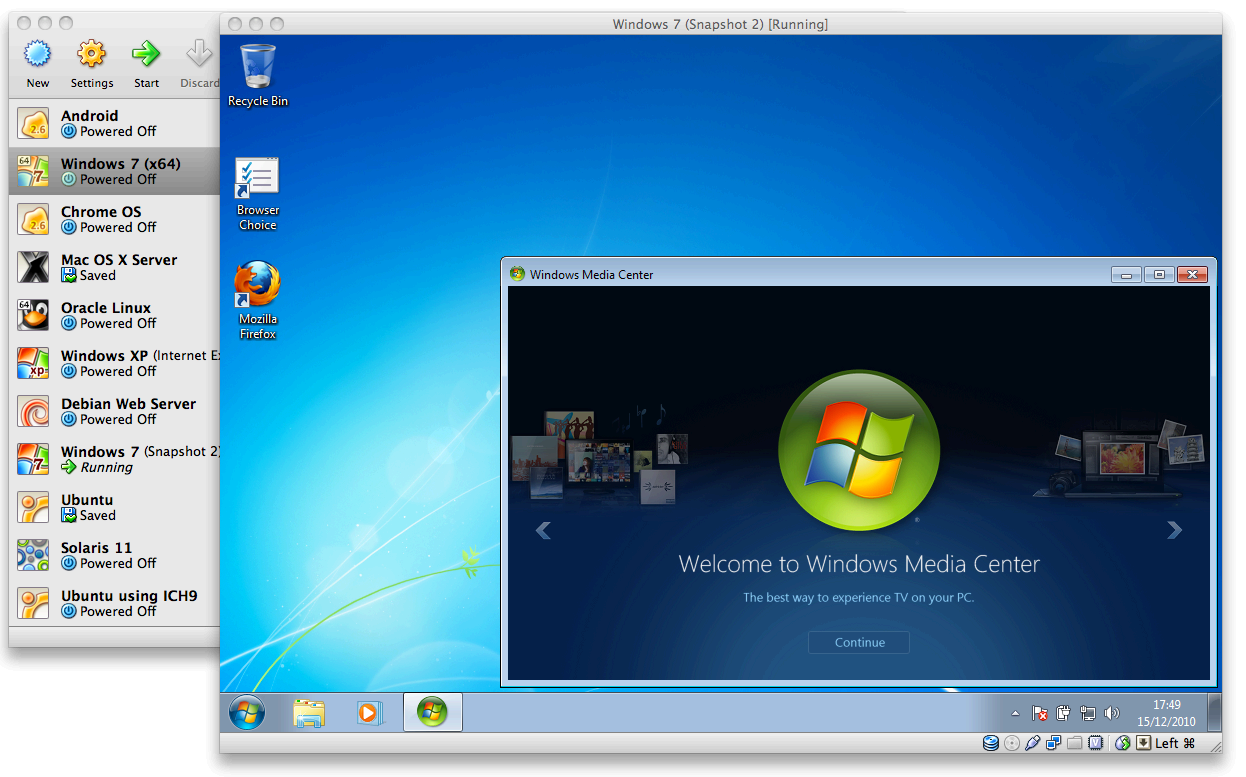
\includegraphics[width=14cm]{images/vm-vista-running.png}
\end{center}

In this User Manual, we'll begin simply with a quick introduction to
  virtualization and how to get your first virtual machine running with the
  easy-to-use VirtualBox graphical user interface. Subsequent chapters will go
  into much more detail covering more powerful tools and features, but
  fortunately, it is not necessary to read the entire User Manual before you
  can use VirtualBox.

You can find a summary of VirtualBox's capabilities in chapter \ref{features-overview}, \textit{\nameref{features-overview}}, page \pageref{features-overview}. For existing VirtualBox users who just want
  to see what's new in this release, there is a detailed list in chapter \ref{ChangeLog}, \textit{\nameref{ChangeLog}}, page \pageref{ChangeLog}.

\section{Why is virtualization useful?}


The techniques and features that VirtualBox provides are useful for
    several scenarios:

\begin{itemize}


\item 

\textbf{Running multiple operating systems
        simultaneously.} VirtualBox allows you to run more than one
        operating system at a time. This way, you can run software written for
        one operating system on another (for example, Windows software on
        Linux or a Mac) without having to reboot to use it. Since you can
        configure what kinds of \OQ{}virtual\CQ{} hardware should be presented to each
        such operating system, you can install an old operating system such as
        DOS or OS/2 even if your real computer's hardware is no longer
        supported by that operating system.


\item 

\textbf{Easier software installations.}
        Software vendors can use virtual machines to ship entire software
        configurations. For example, installing a complete mail server
        solution on a real machine can be a tedious task. With VirtualBox,
        such a complex setup (then often called an \OQ{}appliance\CQ{}) can be packed
        into a virtual machine. Installing and running a mail server becomes
        as easy as importing such an appliance into VirtualBox.


\item 

\textbf{Testing and disaster recovery.}
        Once installed, a virtual machine and its virtual hard disks can be
        considered a \OQ{}container\CQ{} that can be arbitrarily frozen, woken up,
        copied, backed up, and transported between hosts.

On top of that, with the use of another VirtualBox feature
        called \OQ{}snapshots\CQ{}, one can save a particular state of a virtual
        machine and revert back to that state, if necessary. This way, one can
        freely experiment with a computing environment. If something goes
        wrong (e.g. after installing misbehaving software or infecting the
        guest with a virus), one can easily switch back to a previous snapshot
        and avoid the need of frequent backups and restores.

Any number of snapshots can be created, allowing you to travel
        back and forward in virtual machine time. You can delete snapshots
        while a VM is running to reclaim disk space.


\item 

\textbf{Infrastructure consolidation.}
        Virtualization can significantly reduce hardware and electricity
        costs. Most of the time, computers today only use a fraction of their
        potential power and run with low average system loads. A lot of
        hardware resources as well as electricity is thereby wasted. So,
        instead of running many such physical computers that are only
        partially used, one can pack many virtual machines onto a few powerful
        hosts and balance the loads between them.

\end{itemize}


\section{Some terminology}
\label{virtintro}


When dealing with virtualization (and also for understanding the
    following chapters of this documentation), it helps to acquaint oneself
    with a bit of crucial terminology, especially the following terms:

\begin{description}


\item[Host operating system (host OS).]

This is the operating system of the physical computer on which
          VirtualBox was installed. There are versions of VirtualBox for
          Windows, Mac OS X, Linux and Solaris hosts; for details, please see
          chapter \ref{hostossupport}, \textit{\nameref{hostossupport}}, page \pageref{hostossupport}.

Most of the time, this User Manual discusses all VirtualBox
          versions together. There may be platform-specific differences which
          we will point out where appropriate.

\item[Guest operating system (guest OS).]

This is the operating system that is running inside the
          virtual machine. Theoretically, VirtualBox can run any x86 operating
          system (DOS, Windows, OS/2, FreeBSD, OpenBSD), but to achieve
          near-native performance of the guest code on your machine, we had to
          go through a lot of optimizations that are specific to certain
          operating systems. So while your favorite operating system
          \textit{may} run as a guest, we officially support and
          optimize for a select few (which, however, include the most common
          ones).

See chapter \ref{guestossupport}, \textit{\nameref{guestossupport}}, page \pageref{guestossupport} for details.

\item[Virtual machine (VM).]

This is the special environment that VirtualBox creates for
          your guest operating system while it is running. In other words, you
          run your guest operating system \OQ{}in\CQ{} a VM. Normally, a VM will be
          shown as a window on your computer's desktop, but depending on which
          of the various frontends of VirtualBox you use, it can be displayed
          in full screen mode or remotely on another computer.

In a more abstract way, internally, VirtualBox thinks of a VM
          as a set of parameters that determine its behavior. They include
          hardware settings (how much memory the VM should have, what hard
          disks VirtualBox should virtualize through which container files,
          what CDs are mounted etc.) as well as state information (whether the
          VM is currently running, saved, its snapshots etc.). These settings
          are mirrored in the VirtualBox Manager window as well as the
          \texttt{VBoxManage} command line program;
          see chapter \ref{vboxmanage}, \textit{\nameref{vboxmanage}}, page \pageref{vboxmanage}. In other words, a VM is also what
          you can see in its settings dialog.

\item[Guest Additions.]

This refers to special software packages which are shipped
          with VirtualBox but designed to be installed
          \textit{inside} a VM to improve performance of the guest
          OS and to add extra features. This is described in detail in chapter \ref{guestadditions}, \textit{\nameref{guestadditions}}, page \pageref{guestadditions}.
\end{description}


\section{Features overview}
\label{features-overview}


Here's a brief outline of VirtualBox's main features:

\begin{itemize}


\item 

\textbf{Portability.} VirtualBox runs on
        a large number of 32-bit and 64-bit host operating systems (again, see
        chapter \ref{hostossupport}, \textit{\nameref{hostossupport}}, page \pageref{hostossupport} for details).

VirtualBox is a so-called \OQ{}hosted\CQ{} hypervisor (sometimes
        referred to as a \OQ{}type 2\CQ{} hypervisor). Whereas a \OQ{}bare-metal\CQ{} or \OQ{}type
        1\CQ{} hypervisor would run directly on the hardware, VirtualBox requires
        an existing operating system to be installed. It can thus run
        alongside existing applications on that host.

To a very large degree, VirtualBox is functionally identical on
        all of the host platforms, and the same file and image formats are
        used. This allows you to run virtual machines created on one host on
        another host with a different host operating system; for example, you
        can create a virtual machine on Windows and then run it under
        Linux.

In addition, virtual machines can easily be imported and
        exported using the Open Virtualization Format (OVF, see chapter \ref{ovf}, \textit{\nameref{ovf}}, page \pageref{ovf}), an industry standard created for this purpose. You
        can even import OVFs that were created with a different virtualization
        software.


\item 

\textbf{No hardware virtualization
        required.} For many scenarios, VirtualBox does not require
        the processor features built into newer hardware like Intel VT-x or
        AMD-V. As opposed to many other virtualization solutions, you can
        therefore use VirtualBox even on older hardware where these features
        are not present. The technical details are explained in chapter \ref{hwvirt}, \textit{\nameref{hwvirt}}, page \pageref{hwvirt}.


\item 

\textbf{Guest Additions: shared folders, seamless
        windows, 3D virtualization.} The VirtualBox Guest Additions
        are software packages which can be installed
        \textit{inside} of supported guest systems to improve
        their performance and to provide additional integration and
        communication with the host system. After installing the Guest
        Additions, a virtual machine will support automatic adjustment of
        video resolutions, seamless windows, accelerated 3D graphics and more.
        The Guest Additions are described in detail in chapter \ref{guestadditions}, \textit{\nameref{guestadditions}}, page \pageref{guestadditions}.

In particular, Guest Additions provide for \OQ{}shared folders\CQ{},
        which let you access files from the host system from within a guest
        machine. Shared folders are described in chapter \ref{sharedfolders}, \textit{\nameref{sharedfolders}}, page \pageref{sharedfolders}.


\item 

\textbf{Great hardware support.} Among
        others, VirtualBox supports:

\begin{itemize}


\item 

\textbf{Guest multiprocessing
            (SMP).} VirtualBox can present up to 32 virtual CPUs to
            each virtual machine, irrespective of how many CPU cores are
            physically present on your host.


\item 

\textbf{USB device support.}
            VirtualBox implements a virtual USB controller and allows you to
            connect arbitrary USB devices to your virtual machines without
            having to install device-specific drivers on the host. USB support
            is not limited to certain device categories. For details, see
            chapter \ref{settings-usb}, \textit{\nameref{settings-usb}}, page \pageref{settings-usb}.


\item 

\textbf{Hardware compatibility.}
            VirtualBox virtualizes a vast array of virtual devices, among them
            many devices that are typically provided by other virtualization
            platforms. That includes IDE, SCSI and SATA hard disk controllers,
            several virtual network cards and sound cards, virtual serial and
            parallel ports and an Input/Output Advanced Programmable Interrupt
            Controller (I/O APIC), which is found in many modern PC systems.
            This eases cloning of PC images from real machines and importing
            of third-party virtual machines into VirtualBox.


\item 

\textbf{Full ACPI support.} The
            Advanced Configuration and Power Interface (ACPI) is fully
            supported by VirtualBox. This eases cloning of PC images from real
            machines or third-party virtual machines into VirtualBox. With its
            unique \textbf{ACPI power status support,}
            VirtualBox can even report to ACPI-aware guest operating systems
            the power status of the host. For mobile systems running on
            battery, the guest can thus enable energy saving and notify the
            user of the remaining power (e.g. in full screen modes).


\item 

\textbf{Multiscreen resolutions.}
            VirtualBox virtual machines support screen resolutions many times
            that of a physical screen, allowing them to be spread over a large
            number of screens attached to the host system.


\item 

\textbf{Built-in iSCSI support.}
            This unique feature allows you to connect a virtual machine
            directly to an iSCSI storage server without going through the host
            system. The VM accesses the iSCSI target directly without the
            extra overhead that is required for virtualizing hard disks in
            container files. For details, see chapter \ref{storage-iscsi}, \textit{\nameref{storage-iscsi}}, page \pageref{storage-iscsi}.


\item 

\textbf{PXE Network boot.} The
            integrated virtual network cards of VirtualBox fully support
            remote booting via the Preboot Execution Environment (PXE).

\end{itemize}



\item 

\textbf{Multigeneration branched
        snapshots.} VirtualBox can save arbitrary snapshots of the
        state of the virtual machine. You can go back in time and revert the
        virtual machine to any such snapshot and start an alternative VM
        configuration from there, effectively creating a whole snapshot tree.
        For details, see chapter \ref{snapshots}, \textit{\nameref{snapshots}}, page \pageref{snapshots}. You can create and
        delete snapshots while the virtual machine is running.


\item 

\textbf{VM groups.} VirtualBox provides a
        groups feature that enables the user to organize and control virtual machines
        collectively, as well as individually. In addition to basic groups, it
        is also possible for any VM to be in more than one group, and for
        groups to be nested in a hierarchy -- i.e. groups of groups. In
        general, the operations that can be performed on groups are the same as
        those that can be applied to individual VMs i.e. Start, Pause, Reset,
        Close (Save state, Send Shutdown, Poweroff), Discard Saved State, Show
        in fileSystem, Sort.


\item 

\textbf{Clean architecture; unprecedented
        modularity.} VirtualBox has an extremely modular design with
        well-defined internal programming interfaces and a clean separation of
        client and server code. This makes it easy to control it from several
        interfaces at once: for example, you can start a VM simply by clicking
        on a button in the VirtualBox graphical user interface and then
        control that machine from the command line, or even remotely. See
        chapter \ref{frontends}, \textit{\nameref{frontends}}, page \pageref{frontends} for details.

Due to its modular architecture, VirtualBox can also expose its
        full functionality and configurability through a comprehensive
        \textbf{software development kit (SDK),} which
        allows for integrating every aspect of VirtualBox with other software
        systems. Please see chapter \ref{VirtualBoxAPI}, \textit{\nameref{VirtualBoxAPI}}, page \pageref{VirtualBoxAPI} for
        details.


\item 

\textbf{Remote machine display.} The
        VirtualBox Remote Desktop Extension (VRDE) allows for high-performance
        remote access to any running virtual machine. This extension supports
        the Remote Desktop Protocol (RDP) originally built into Microsoft
        Windows, with special additions for full client USB support.

The VRDE does not rely on the RDP server that is built into
        Microsoft Windows; instead, it is plugged directly into the
        virtualization layer. As a result, it works with guest operating
        systems other than Windows (even in text mode) and does not require
        application support in the virtual machine either. The VRDE is
        described in detail in chapter \ref{vrde}, \textit{\nameref{vrde}}, page \pageref{vrde}.

On top of this special capacity, VirtualBox offers you more
        unique features:

\begin{itemize}


\item 

\textbf{Extensible RDP
              authentication.} VirtualBox already supports Winlogon
              on Windows and PAM on Linux for RDP authentication. In addition,
              it includes an easy-to-use SDK which allows you to create
              arbitrary interfaces for other methods of authentication; see
              chapter \ref{vbox-auth}, \textit{\nameref{vbox-auth}}, page \pageref{vbox-auth} for details.


\item 

\textbf{USB over RDP.} Via RDP
              virtual channel support, VirtualBox also allows you to connect
              arbitrary USB devices locally to a virtual machine which is
              running remotely on a VirtualBox RDP server; see chapter \ref{usb-over-rdp}, \textit{\nameref{usb-over-rdp}}, page \pageref{usb-over-rdp} for details.

\end{itemize}


\end{itemize}


\section{Supported host operating systems}
\label{hostossupport}


Currently, VirtualBox runs on the following host operating
    systems:

\begin{itemize}


\item 

\textbf{Windows} hosts:

\begin{itemize}


\item 

Windows XP, all service packs (32-bit)


\item 

Windows Server 2003 (32-bit)


\item 

Windows Vista (32-bit and 64-bit\footnote{Support for 64-bit Windows was added with VirtualBox
                  1.5.}).


\item 

Windows Server 2008 (32-bit and 64-bit)


\item 

Windows 7 (32-bit and 64-bit)


\item 

Windows 8 (32-bit and 64-bit)


\item 

Windows Server 2012 (64-bit)

\end{itemize}



\item 

\textbf{Mac OS X} hosts:\footnote{Preliminary Mac OS X support (beta stage) was added with
            VirtualBox 1.4, full support with 1.6. Mac OS X 10.4 (Tiger)
            support was removed with VirtualBox 3.1.}

\begin{itemize}


\item 

10.6 (Snow Leopard, 32-bit and 64-bit)


\item 

10.7 (Lion, 32-bit and 64-bit)


\item 

10.8 (Mountain Lion, 64-bit)


\item 

10.9 (Mavericks, 64-bit)

\end{itemize}


Intel hardware is required; please see chapter \ref{KnownIssues}, \textit{\nameref{KnownIssues}}, page \pageref{KnownIssues} also.


\item 

\textbf{Linux} hosts (32-bit and
        64-bit\footnote{Support for 64-bit Linux was added with VirtualBox
            1.4.}). Among others, this includes:

\begin{itemize}


\item 

10.04 (\OQ{}Lucid Lynx\CQ{}), 10.10 (\OQ{}Maverick Meerkat),
              11.04 (\OQ{}Natty Narwhal\CQ{}), 11.10 (\OQ{}Oneiric Oncelot\CQ{}),
              12.04 (\OQ{}Precise Pangolin\CQ{}), 12.10 (\OQ{}Quantal Quetzal\CQ{}),
              13.04 (\OQ{}Raring Ringtail\CQ{}), 13.10 (\OQ{}Saucy Salamander\CQ{})


\item 

Debian GNU/Linux 6.0 (\OQ{}squeeze\CQ{}) and 7.0 (\OQ{}wheezy\CQ{})


\item 

Oracle Enterprise Linux 5, Oracle Linux 6


\item 

Redhat Enterprise Linux 5 and 6


\item 

Fedora Core 6 to 19


\item 

Gentoo Linux


\item 

openSUSE 11.0, 11.1, 11.2, 11.3, 11.4, 12.1, 12.2


\item 

Mandriva 2010 and 2011

\end{itemize}


It should be possible to use VirtualBox on most systems based on
        Linux kernel 2.6 or 3.x using either the VirtualBox installer or by doing a
        manual installation; see chapter \ref{install-linux-host}, \textit{\nameref{install-linux-host}}, page \pageref{install-linux-host}. However,
        the formally tested and supported Linux distributions are those for
        which we offer a dedicated package.

Note that starting with VirtualBox 2.1, Linux 2.4-based host
        operating systems are no longer supported.


\item 

\textbf{Solaris} hosts (64-bit only) are
        supported with the restrictions listed in chapter \ref{KnownIssues}, \textit{\nameref{KnownIssues}}, page \pageref{KnownIssues}:

\begin{itemize}


\item 

Solaris 11 including Solaris 11 Express


\item 

Solaris 10 (u8 and higher)

\end{itemize}


\end{itemize}


Note that the above list is informal. Oracle support for customers
    who have a support contract is limited to a subset of the listed host
    operating systems. Also, any feature which is marked as  \textbf{experimental} is not supported. Feedback and
    suggestions about such features are welcome.

\section{Installing VirtualBox and extension packs}
\label{intro-installing}


VirtualBox comes in many different packages, and installation
    depends on your host operating system. If you have installed software
    before, installation should be straightforward: on each host platform,
    VirtualBox uses the installation method that is most common and easy to
    use. If you run into trouble or have special requirements, please refer to
    chapter \ref{installation}, \textit{\nameref{installation}}, page \pageref{installation} for details about the various installation
    methods.

Starting with version 4.0, VirtualBox is split into several
    components.

\begin{enumerate}


\item 

The base package consists of all open-source components and is
          licensed under the GNU General Public License V2.


\item 

Additional extension packs can be downloaded which extend the
          functionality of the VirtualBox base package. Currently, Oracle
          provides the one extension pack, which can be found at \url{http://www.virtualbox.org}
          and provides the following added functionality:

\begin{enumerate}


\item 

The virtual USB 2.0 (EHCI) device; see chapter \ref{settings-usb}, \textit{\nameref{settings-usb}}, page \pageref{settings-usb}.


\item 

VirtualBox Remote Desktop Protocol (VRDP) support; see
                chapter \ref{vrde}, \textit{\nameref{vrde}}, page \pageref{vrde}.


\item 

Host webcam passthrough; see chapter chapter \ref{webcam-passthrough}, \textit{\nameref{webcam-passthrough}}, page \pageref{webcam-passthrough}.


\item 

Intel PXE boot ROM.


\item 

Experimental support for PCI passthrough on Linux hosts;
                  see chapter \ref{pcipassthrough}, \textit{\nameref{pcipassthrough}}, page \pageref{pcipassthrough}.

\end{enumerate}


VirtualBox extension packages have a
          \texttt{.vbox-extpack} file name extension.
          To install an extension, simply double-click on the package file
          and a Network Operations Manager window will appear, guiding you
          through the required steps.

To view the extension packs that are currently installed,
          please start the VirtualBox Manager (see the next section). From the
          \OQ{}File\CQ{} menu, please select \OQ{}Preferences\CQ{}. In the window that shows
          up, go to the \OQ{}Extensions\CQ{} category which shows you the extensions
          which are currently installed and allows you to remove a package or
          add a new one.

Alternatively you can use VBoxManage on the command line: see
          chapter \ref{vboxmanage-extpack}, \textit{\nameref{vboxmanage-extpack}}, page \pageref{vboxmanage-extpack} for details.

\end{enumerate}


\section{Starting VirtualBox}


After installation, you can start VirtualBox as
    follows:

\begin{itemize}


\item 

On a Windows host, in the standard \OQ{}Programs\CQ{} menu, click on
          the item in the \OQ{}VirtualBox\CQ{} group. On Vista or Windows 7, you can
          also type \OQ{}VirtualBox\CQ{} in the search box of the \OQ{}Start\CQ{} menu.


\item 

On a Mac OS X host, in the Finder, double-click on the
          \OQ{}VirtualBox\CQ{} item in the \OQ{}Applications\CQ{} folder. (You may want to
          drag this item onto your Dock.)


\item 

On a Linux or Solaris host, depending on your desktop
          environment, a \OQ{}VirtualBox\CQ{} item may have been placed in either the
          \OQ{}System\CQ{} or \OQ{}System Tools\CQ{} group of your \OQ{}Applications\CQ{} menu.
          Alternatively, you can type
          \texttt{VirtualBox} in a terminal.

\end{itemize}


When you start VirtualBox for the first time, a window like the
    following should come up:

\begin{center}
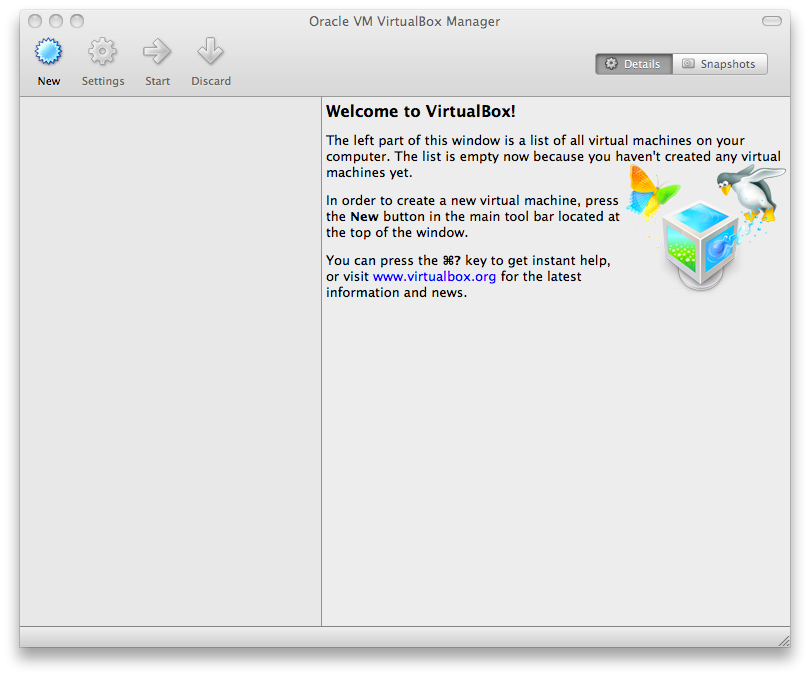
\includegraphics[width=10cm]{images/virtualbox-main-empty.png}
\end{center}This window is called the \textbf{\OQ{}VirtualBox Manager\CQ{}.} On the left, you can see a
    pane that will later list all your virtual machines. Since you have not
    created any, the list is empty. A row of buttons above it allows you to
    create new VMs and work on existing VMs, once you have some. The pane on
    the right displays the properties of the virtual machine currently
    selected, if any. Again, since you don't have any machines yet, the pane
    displays a welcome message.

To give you an idea what VirtualBox might look like later, after you
    have created many machines, here's another example:

\begin{center}
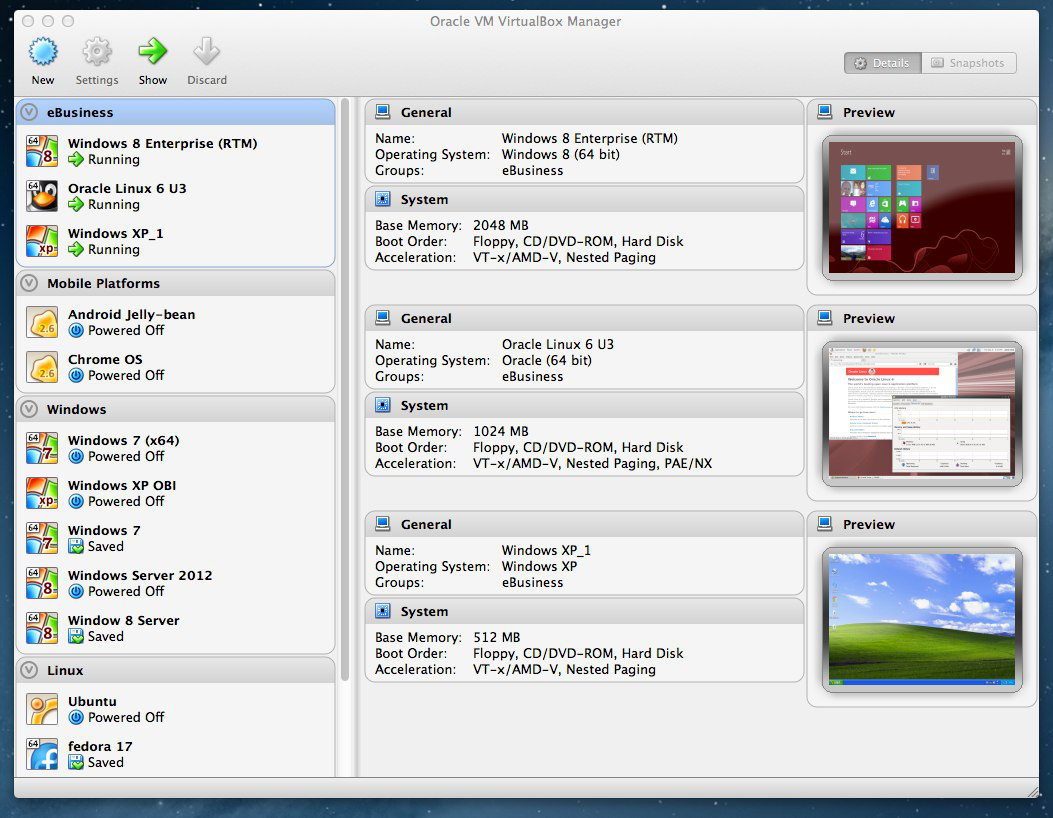
\includegraphics[width=10cm]{images/virtualbox-main.png}
\end{center}

\section{Creating your first virtual machine}
\label{gui-createvm}


Click on the \OQ{}New\CQ{} button at the top of the VirtualBox Manager
    window. A wizard will pop up to guide you through setting up a new virtual
    machine (VM):

\begin{center}
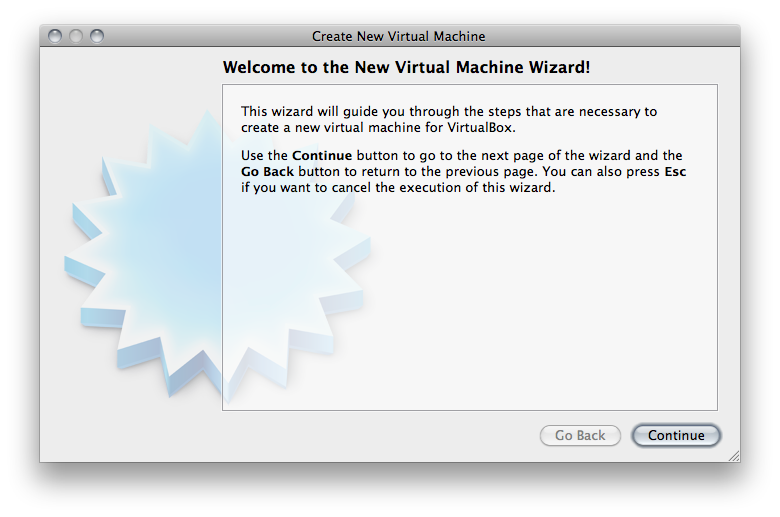
\includegraphics[width=10cm]{images/create-vm-1.png}
\end{center}On the following pages, the wizard will ask you for the
    bare minimum of information that is needed to create a VM, in
    particular:

\begin{enumerate}


\item 

The \textbf{VM name} will later be
          shown in the VM list of the VirtualBox Manager window, and it will
          be used for the VM's files on disk. Even though any name could be
          used, keep in mind that once you have created a few VMs, you will
          appreciate if you have given your VMs rather informative names; \OQ{}My
          VM\CQ{} would thus be less useful than \OQ{}Windows XP SP2 with
          OpenOffice\CQ{}.


\item 

For \textbf{\OQ{}Operating System Type\CQ{},}
          select the operating system that you want to install later. The
          supported operating systems are grouped; if you want to install
          something very unusual that is not listed, select \OQ{}Other\CQ{}. Depending
          on your selection, VirtualBox will enable or disable certain VM
          settings that your guest operating system may require. This is
          particularly important for 64-bit guests (see chapter \ref{intro-64bitguests}, \textit{\nameref{intro-64bitguests}}, page \pageref{intro-64bitguests}). It is therefore recommended to
          always set it to the correct value.


\item 

On the next page, select the \textbf{memory
          (RAM)} that VirtualBox should allocate every time the
          virtual machine is started. The amount of memory given here will be
          taken away from your host machine and presented to the guest
          operating system, which will report this size as the (virtual)
          computer's installed RAM.



\vspace{.2cm}

\begin{center}\fbox{\begin{minipage}[c]{0.9\textwidth}\color{colNote}\textbf{Note:} Choose this setting carefully! The memory you give to the
              VM will not be available to your host OS while the VM is
              running, so do not specify more than you can spare. For example,
              if your host machine has 1 GB of RAM and you enter 512 MB as the
              amount of RAM for a particular virtual machine, while that VM is
              running, you will only have 512 MB left for all the other
              software on your host. If you run two VMs at the same time, even
              more memory will be allocated for the second VM (which may not
              even be able to start if that memory is not available). On the
              other hand, you should specify as much as your guest OS (and
              your applications) will require to run properly.\end{minipage}}\end{center}

\vspace{.2cm}



A Windows XP guest will require at least a few hundred MB RAM
          to run properly, and Windows Vista will even refuse to install with
          less than 512 MB. Of course, if you want to run graphics-intensive
          applications in your VM, you may require even more RAM.

So, as a rule of thumb, if you have 1 GB of RAM or more in
          your host computer, it is usually safe to allocate 512 MB to each
          VM. But, in any case, make sure you always have at least 256 to 512
          MB of RAM left on your host operating system. Otherwise you may
          cause your host OS to excessively swap out memory to your hard disk,
          effectively bringing your host system to a standstill.

As with the other settings, you can change this setting later,
          after you have created the VM.


\item 

Next, you must specify a \textbf{virtual hard
          disk} for your VM.

There are many and potentially complicated ways in which
          VirtualBox can provide hard disk space to a VM (see chapter \ref{storage}, \textit{\nameref{storage}}, page \pageref{storage} for details), but the most common way is to use
          a large image file on your \OQ{}real\CQ{} hard disk, whose contents
          VirtualBox presents to your VM as if it were a complete hard disk.
          This file represents an entire hard disk then, so you can even copy
          it to another host and use it with another VirtualBox
          installation.

The wizard shows you the following window:

\begin{center}
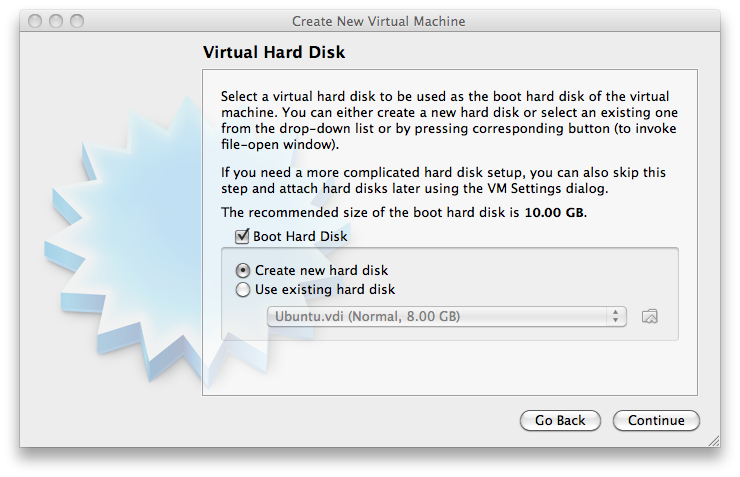
\includegraphics[width=10cm]{images/create-vm-2.png}
\end{center}

Here you have the following options:



\begin{itemize}


\item 

To create a new, empty virtual hard disk, press the
                \textbf{\OQ{}New\CQ{}} button.


\item 

You can pick an \textbf{existing} disk image file.

The \textbf{drop-down list}
                presented in the window contains all disk images which are
                currently remembered by VirtualBox, probably because they are
                currently attached to a virtual machine (or have been in the
                past).

Alternatively, you can click on the small \textbf{folder button} next to the drop-down
                list to bring up a standard file dialog, which allows you to
                pick any disk image file on your host disk.

\end{itemize}
Most probably, if you are using VirtualBox for the
          first time, you will want to create a new disk image. Hence, press
          the \OQ{}New\CQ{} button.

This brings up another window, the \textbf{\OQ{}Create New Virtual Disk Wizard\CQ{},} which helps
          you create a new disk image file in the new virtual machine's
          folder.

VirtualBox supports two types of image files:

\begin{itemize}


\item 

A \textbf{dynamically allocated
                file} will only grow in size when the guest actually
                stores data on its virtual hard disk. It will therefore
                initially be small on the host hard drive and only later grow
                to the size specified as it is filled with data.


\item 

A \textbf{fixed-size file} will
                immediately occupy the file specified, even if only a fraction
                of the virtual hard disk space is actually in use. While
                occupying much more space, a fixed-size file incurs less
                overhead and is therefore slightly faster than a dynamically
                allocated file.

\end{itemize}


For details about the differences, please refer to chapter \ref{vdidetails}, \textit{\nameref{vdidetails}}, page \pageref{vdidetails}.

To prevent your physical hard disk from running full,
          VirtualBox limits the size of the image file. Still, it needs to be
          large enough to hold the contents of your operating system and the
          applications you want to install -- for a modern Windows or Linux
          guest, you will probably need several gigabytes for any serious
          use. The limit of the image file size can be changed later (see chapter \ref{vboxmanage-modifyvdi}, \textit{\nameref{vboxmanage-modifyvdi}}, page \pageref{vboxmanage-modifyvdi} for details).\begin{center}
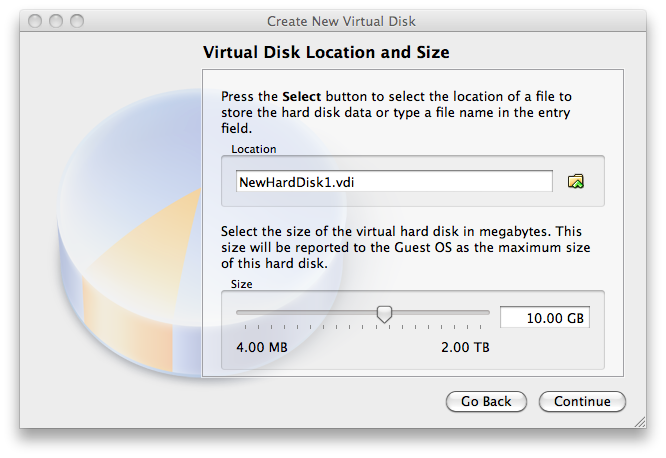
\includegraphics[width=10cm]{images/create-vdi-1.png}
\end{center}

After having selected or created your image file, again press
          \textbf{\OQ{}Next\CQ{}} to go to the next
          page.


\item 

After clicking on \textbf{\OQ{}Finish\CQ{}},
          your new virtual machine will be created. You will then see it in
          the list on the left side of the Manager window, with the name you
          entered initially.

\end{enumerate}


\vspace{.2cm}

\begin{center}\fbox{\begin{minipage}[c]{0.9\textwidth}\color{colNote}\textbf{Note:} After becoming familiar with the use of wizards, consider using
      the Expert Mode available in some wizards. Where available, this is
      selectable using a button, and speeds up user processes using
      wizards.\end{minipage}}\end{center}

\vspace{.2cm}



\section{Running your virtual machine}


To start a virtual machine, you have several options:

\begin{itemize}


\item 

Double-click on its entry in the list within the Manager
          window or


\item 

select its entry in the list in the Manager window it and
          press the \OQ{}Start\CQ{} button at the top or


\item 

for virtual machines created with VirtualBox 4.0 or later,
          navigate to the \OQ{}VirtualBox VMs\CQ{} folder in your system user's home
          directory, find the subdirectory of the machine you want to start
          and double-click on the machine settings file (with a
          \texttt{.vbox} file extension).

\end{itemize}


This opens up a new window, and the virtual machine which you
    selected will boot up. Everything which would normally be seen on the
    virtual system's monitor is shown in the window, as can be seen with the
    image in chapter \ref{virtintro}, \textit{\nameref{virtintro}}, page \pageref{virtintro}.

In general, you can use the virtual machine much like you would use
    a real computer. There are couple of points worth mentioning
    however.

\subsection{Starting a new VM for the first time}


When a VM gets started for the first time, another wizard -- the
      \textbf{\OQ{}First Start Wizard\CQ{}} -- will pop up to
      help you select an \textbf{installation medium}.
      Since the VM is created empty, it would otherwise behave just like a
      real computer with no operating system installed: it will do nothing and
      display an error message that no bootable operating system was
      found.

For this reason, the wizard helps you select a medium to install
      an operating system from.

\begin{itemize}


\item 

If you have physical CD or DVD media from which you want to
          install your guest operating system (e.g. in the case of a Windows
          installation CD or DVD), put the media into your host's CD or DVD
          drive.

Then, in the wizard's drop-down list of installation media,
          select \textbf{\OQ{}Host drive\CQ{}} with the
          correct drive letter (or, in the case of a Linux host, device file).
          This will allow your VM to access the media in your host drive, and
          you can proceed to install from there.


\item 

If you have downloaded installation media from the Internet in
          the form of an ISO image file (most probably in the case of a Linux
          distribution), you would normally burn this file to an empty CD or
          DVD and proceed as just described. With VirtualBox however, you can
          skip this step and mount the ISO file directly. VirtualBox will then
          present this file as a CD or DVD-ROM drive to the virtual machine,
          much like it does with virtual hard disk images.

For this case, the wizard's drop-down list contains a list of
          installation media that were previously used with VirtualBox.

If your medium is not in the list (especially if you are using
          VirtualBox for the first time), select the small folder icon next to
          the drop-down list to bring up a standard file dialog, with which
          you can pick the image file on your host disks.

\end{itemize}


In both cases, after making the choices in the wizard, you will be
      able to install your operating system.

\subsection{Capturing and releasing keyboard and mouse}
\label{keyb_mouse_normal}


As of version 3.2, VirtualBox provides a virtual USB tablet device
      to new virtual machines through which mouse events are communicated to
      the guest operating system. As a result, if you are running a modern
      guest operating system that can handle such devices, mouse support may
      work out of the box without the mouse being \OQ{}captured\CQ{} as described
      below; see chapter \ref{settings-motherboard}, \textit{\nameref{settings-motherboard}}, page \pageref{settings-motherboard} for more
      information.

Otherwise, if the virtual machine only sees standard PS/2 mouse
      and keyboard devices, since the operating system in the virtual machine
      does not \OQ{}know\CQ{} that it is not running on a real computer, it expects to
      have exclusive control over your keyboard and mouse. This is, however,
      not the case since, unless you are running the VM in full screen mode,
      your VM needs to share keyboard and mouse with other applications and
      possibly other VMs on your host.

As a result, initially after installing a guest operating system
      and before you install the Guest Additions (we will explain this in a
      minute), only one of the two -- your VM or the rest of your computer --
      can \OQ{}own\CQ{} the keyboard and the mouse. You will see a
      \textit{second} mouse pointer which will always be confined
      to the limits of the VM window. Basically, you activate the VM by
      clicking inside it.

To return ownership of keyboard and mouse to your host operating
      system, VirtualBox reserves a special key on your keyboard for itself:
      the \textbf{\OQ{}host key\CQ{}.} By default, this is the
      \textit{right Control key} on your keyboard; on a Mac host,
      the default host key is the left Command key. You can change this
      default in the VirtualBox Global Settings, see chapter \ref{globalsettings}, \textit{\nameref{globalsettings}}, page \pageref{globalsettings}. In any case, the current
      setting for the host key is always displayed \textit{at the bottom
      right of your VM window,} should you have forgotten about
      it:

\begin{center}

\includegraphics[width=7cm]{images/vm-hostkey.png}
\end{center}In detail, all this translates into the
      following:



\begin{itemize}


\item 

Your \textbf{keyboard} is owned by
            the VM if the VM window on your host desktop has the keyboard
            focus (and then, if you have many windows open in your guest
            operating system as well, the window that has the focus in your
            VM). This means that if you want to type within your VM, click on
            the title bar of your VM window first.

To release keyboard ownership, press the Host key (as
            explained above, typically the right Control key).

Note that while the VM owns the keyboard, some key sequences
            (like Alt-Tab for example) will no longer be seen by the host, but
            will go to the guest instead. After you press the host key to
            re-enable the host keyboard, all key presses will go through the
            host again, so that sequences like Alt-Tab will no longer reach
            the guest.  For technical reasons it may not be possible for the
            VM to get all keyboard input even when it does own the keyboard.
            Examples of this are the Ctrl-Alt-Del sequence on Windows hosts
            or single keys grabbed by other applications on X11 hosts like
            the GNOME desktop's \OQ{}Control key highlights mouse pointer\CQ{}
            functionality.


\item 

Your \textbf{mouse} is owned by the
            VM only after you have clicked in the VM window. The host mouse
            pointer will disappear, and your mouse will drive the guest's
            pointer instead of your normal mouse pointer.

Note that mouse ownership is independent of that of the
            keyboard: even after you have clicked on a titlebar to be able to
            type into the VM window, your mouse is not necessarily owned by
            the VM yet.

To release ownership of your mouse by the VM, also press the
            Host key.

\end{itemize}


As this behavior can be inconvenient, VirtualBox provides a set of
      tools and device drivers for guest systems called the \OQ{}VirtualBox Guest
      Additions\CQ{} which make VM keyboard and mouse operation a lot more
      seamless. Most importantly, the Additions will get rid of the second
      \OQ{}guest\CQ{} mouse pointer and make your host mouse pointer work directly in
      the guest.

This will be described later in chapter \ref{guestadditions}, \textit{\nameref{guestadditions}}, page \pageref{guestadditions}.

\subsection{Typing special characters}
\label{specialcharacters}


Operating systems expect certain key combinations to initiate
      certain procedures. Some of these key combinations may be difficult to
      enter into a virtual machine, as there are three candidates as to who
      receives keyboard input: the host operating system, VirtualBox, or the
      guest operating system. Who of these three receives keypresses depends
      on a number of factors, including the key itself.

\begin{itemize}


\item 

Host operating systems reserve certain key combinations for
          themselves. For example, it is impossible to enter the \textbf{Ctrl+Alt+Delete} combination if you want to
          reboot the guest operating system in your virtual machine, because
          this key combination is usually hard-wired into the host OS (both
          Windows and Linux intercept this), and pressing this key combination
          will therefore reboot your \textit{host}.

Also, on Linux and Solaris hosts, which use the X Window
          System, the key combination \textbf{Ctrl+Alt+Backspace} normally resets the X
          server (to restart the entire graphical user interface in case it
          got stuck). As the X server intercepts this combination, pressing it
          will usually restart your \textit{host} graphical user
          interface (and kill all running programs, including VirtualBox, in
          the process).

Third, on Linux hosts supporting virtual terminals, the key
          combination \textbf{Ctrl+Alt+Fx} (where Fx
          is one of the function keys from F1 to F12) normally allows to
          switch between virtual terminals. As with Ctrl+Alt+Delete, these
          combinations are intercepted by the host operating system and
          therefore always switch terminals on the
          \textit{host}.

If, instead, you want to send these key combinations to the
          \textit{guest} operating system in the virtual machine,
          you will need to use one of the following methods:

\begin{itemize}


\item 

Use the items in the \OQ{}Machine\CQ{} menu of the virtual machine
              window. There you will find \OQ{}Insert Ctrl+Alt+Delete\CQ{} and
              \OQ{}Ctrl+Alt+Backspace\CQ{}; the latter will only have an effect with
              Linux or Solaris guests, however.


\item 

Press special key combinations with the Host key (normally
              the right Control key), which VirtualBox will then translate for
              the virtual machine:

\begin{itemize}


\item 

\textbf{Host key + Del} to
                    send Ctrl+Alt+Del (to reboot the guest);


\item 

\textbf{Host key +
                    Backspace} to send Ctrl+Alt+Backspace (to
                    restart the graphical user interface of a Linux or Solaris
                    guest);


\item 

\textbf{Host key + F1} (or
                    other function keys) to simulate Ctrl+Alt+F1 (or other
                    function keys, i.e. to switch between virtual terminals in
                    a Linux guest).

\end{itemize}


\end{itemize}



\item 

For some other keyboard combinations such as \textbf{Alt-Tab} (to switch between open windows),
          VirtualBox allows you to configure whether these combinations will
          affect the host or the guest, if a virtual machine currently has the
          focus. This is a global setting for all virtual machines and can be
          found under \OQ{}File\CQ{} -> \OQ{}Preferences\CQ{} -> \OQ{}Input\CQ{} ->
          \OQ{}Auto-capture keyboard\CQ{}.

\end{itemize}


\subsection{Changing removable media}


While a virtual machine is running, you can change removable media
      in the \OQ{}Devices\CQ{} menu of the VM's window. Here you can select in detail
      what VirtualBox presents to your VM as a CD, DVD, or floppy.

The settings are the same as would be available for the VM in the
      \OQ{}Settings\CQ{} dialog of the VirtualBox main window, but since that dialog
      is disabled while the VM is in the \OQ{}running\CQ{} or \OQ{}saved\CQ{} state, this
      extra menu saves you from having to shut down and restart the VM every
      time you want to change media.

Hence, in the \OQ{}Devices\CQ{} menu, VirtualBox allows you to attach the
      host drive to the guest or select a floppy or DVD image using the Disk
      Image Manager, all as described in chapter \ref{configbasics}, \textit{\nameref{configbasics}}, page \pageref{configbasics}.

\subsection{Resizing the machine's window}
\label{intro-resize-window}


You can resize the virtual machine's window when it is running. In
      that case, one of three things will happen:

\begin{enumerate}


\item 

If you have \textbf{\OQ{}scale mode\CQ{}}
            enabled, then the virtual machine's screen will be scaled to the
            size of the window. This can be useful if you have many machines
            running and want to have a look at one of them while it is running
            in the background. Alternatively, it might be useful to enlarge a
            window if the VM's output screen is very small, for example
            because you are running an old operating system in it.

To enable scale mode, press the \textbf{host
            key + C}, or select \OQ{}Scale mode\CQ{} from the \OQ{}Machine\CQ{} menu
            in the VM window. To leave scale mode, press the host key + C
            again.

The aspect ratio of the guest screen is preserved when
            resizing the window. To ignore the aspect ratio, press Shift
            during the resize operation.

Please see chapter \ref{KnownIssues}, \textit{\nameref{KnownIssues}}, page \pageref{KnownIssues} for additional
            remarks.


\item 

If you have the Guest Additions installed and they support
            automatic \textbf{resizing}, the Guest
            Additions will automatically adjust the screen resolution of the
            guest operating system. For example, if you are running a Windows
            guest with a resolution of 1024x768 pixels and you then resize the
            VM window to make it 100 pixels wider, the Guest Additions will
            change the Windows display resolution to 1124x768.

Please see chapter \ref{guestadditions}, \textit{\nameref{guestadditions}}, page \pageref{guestadditions} for more
            information about the Guest Additions.


\item 

Otherwise, if the window is bigger than the VM's screen, the
            screen will be centered. If it is smaller, then scroll bars will
            be added to the machine window.

\end{enumerate}


\subsection{Saving the state of the machine}


When you click on the \OQ{}Close\CQ{} button of your virtual machine
      window (at the top right of the window, just like you would close any
      other window on your system), VirtualBox asks you whether you want to
      \OQ{}save\CQ{} or \OQ{}power off\CQ{} the VM. (As a shortcut, you can also press the
      Host key together with \OQ{}Q\CQ{}.)

\begin{center}
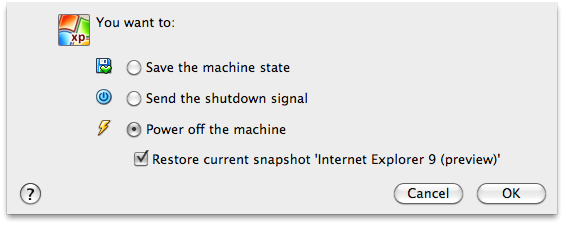
\includegraphics[width=11cm]{images/vm-close.png}
\end{center}The difference between these three options is crucial.
      They mean:

\begin{itemize}


\item 

\textbf{Save the machine state:} With
          this option, VirtualBox \OQ{}freezes\CQ{} the virtual machine by completely
          saving its state to your local disk.

When you start the VM again later, you will find that the VM
          continues exactly where it was left off. All your programs will
          still be open, and your computer resumes operation. Saving the state
          of a virtual machine is thus in some ways similar to suspending a
          laptop computer (e.g. by closing its lid).


\item 

\textbf{Send the shutdown signal.}
          This will send an ACPI shutdown signal to the virtual machine, which
          has the same effect as if you had pressed the power button on a real
          computer. So long as the VM is running a fairly modern operating
          system, this should trigger a proper shutdown mechanism from within
          the VM.


\item 

\textbf{Power off the machine:} With
          this option, VirtualBox also stops running the virtual machine, but
          \textit{without} saving its state.

\vspace{.2cm}

\begin{center}\fbox{\begin{minipage}[c]{0.9\textwidth}\color{colWarning}\textbf{Warning:} This is equivalent to pulling the power plug on a real
              computer without shutting it down properly. If you start the
              machine again after powering it off, your operating system will
              have to reboot completely and may begin a lengthy check of its
              (virtual) system disks. As a result, this should not normally be
              done, since it can potentially cause data loss or an
              inconsistent state of the guest system on disk.\end{minipage}}\end{center}

\vspace{.2cm}



As an exception, if your virtual machine has any snapshots
          (see the next chapter), you can use this option to quickly \textbf{restore the current snapshot} of the virtual
          machine. In that case, powering off the machine will not disrupt its
          state, but any changes made since that snapshot was taken will be
          lost.

\end{itemize}


The \textbf{\OQ{}Discard\CQ{}} button in the
      VirtualBox Manager window discards a virtual machine's saved state. This
      has the same effect as powering it off, and the same warnings
      apply.

\section{Using VM groups}
\label{gui-vmgroups}


VM groups enable the user to create ad hoc groups of VMs, and to 
    manage and perform functions on them collectively, as well as individually. 
    There are a number of features relating to groups:

\begin{enumerate}


\item 


            Create a group using GUI option 1) Drag one VM on top of another
            VM. 
          


            Create a group using GUI option 2) Select multiple VMs and select
            \OQ{}Group\CQ{} on the right click menu, as follows:
          

\begin{center}
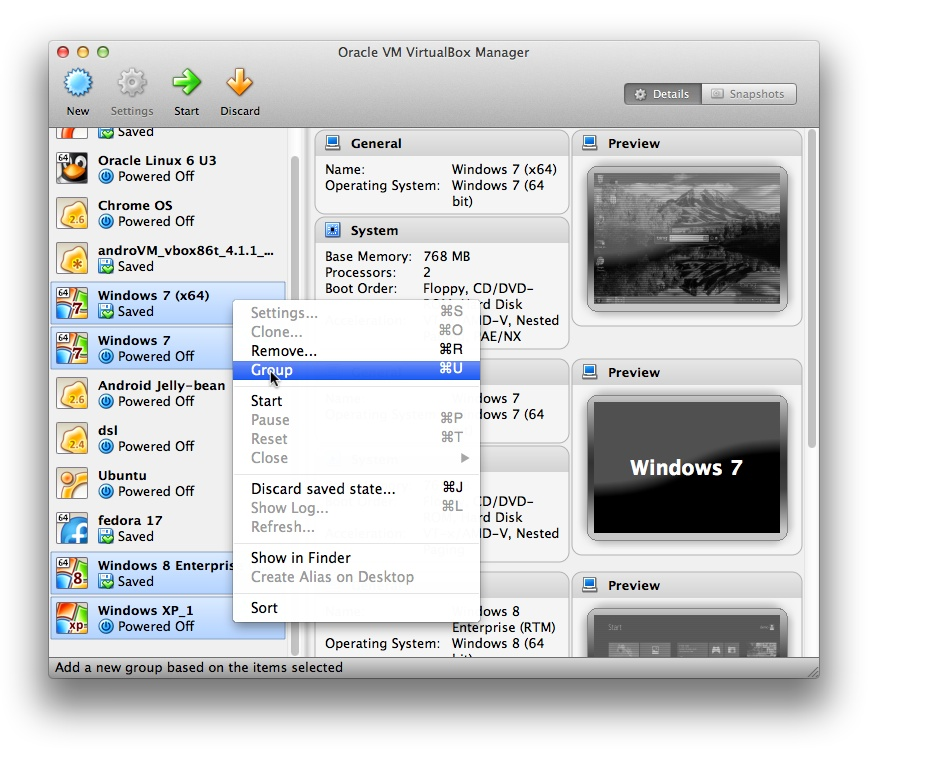
\includegraphics[width=10cm]{images/vm-groups.png}
\end{center}


\item 


            Command line option 1) Create a group and assign a VM:
            

\begin{Verbatim}[fontsize=\footnotesize]
VBoxManage modifyvm "Fred" --groups "/TestGroup"
\end{Verbatim}

            creates a group \OQ{}TestGroup\CQ{} and attaches the VM \OQ{}Fred\CQ{} to that group.
          


            Command line option 2) Detach a VM from the group, and delete the group
            if empty: 

\begin{Verbatim}[fontsize=\footnotesize]
VBoxManage modifyvm "Fred" --groups ""
\end{Verbatim}

            It detaches all groups from the VM \OQ{}Fred\CQ{} and deletes the empty group.
          


\item 


            Multiple groups e.g.:
            

\begin{Verbatim}[fontsize=\footnotesize]
VBoxManage modifyvm "Fred" --groups "/TestGroup,/TestGroup2"
\end{Verbatim}

            It creates the groups \OQ{}TestGroup\CQ{} and \OQ{}TestGroup2\CQ{} (if they don't exist yet)
            and attaches the VM \OQ{}Fred\CQ{} to both of them.
          


\item 


            Nested groups -- hierarchy of groups e.g.:
            

\begin{Verbatim}[fontsize=\footnotesize]
VBoxManage modifyvm "Fred" --groups "/TestGroup/TestGroup2"
\end{Verbatim}

            It attaches the VM \OQ{}Fred\CQ{} to the subgroup \OQ{}TestGroup2\CQ{} of the \OQ{}TestGroup\CQ{}
            group.
          


\item 


          Summary of group commands: Start, Pause, Reset, Close (save state,
          send shutdown signal, poweroff), Discard Saved State, Show in File
          System, Sort.
          

\end{enumerate}


\section{Snapshots}
\label{snapshots}


With snapshots, you can save a particular state of a virtual machine
    for later use. At any later time, you can revert to that state, even
    though you may have changed the VM considerably since then. A snapshot of
    a virtual machine is thus similar to a machine in \OQ{}saved\CQ{} state, as
    described above, but there can be many of them, and these saved states are
    preserved.

You can see the snapshots of a virtual machine by first selecting a
    machine in the VirtualBox Manager and then clicking on the \OQ{}Snapshots\CQ{}
    button at the top right. Until you take a snapshot of the machine, the
    list of snapshots will be empty except for the \OQ{}Current state\CQ{} item, which
    represents the \OQ{}Now\CQ{} point in the lifetime of the virtual machine.

\subsection{Taking, restoring and deleting snapshots}


There are three operations related to snapshots:

\begin{enumerate}


\item 

You can \textbf{take a snapshot}.
            This makes a copy of the machine's current state, to which you can
            go back at any given time later.

\begin{itemize}


\item 

If your VM is currently running, select \OQ{}Take
                  snapshot\CQ{} from the \OQ{}Machine\CQ{} pull-down menu of the VM
                  window.


\item 

If your VM is currently in either the \OQ{}saved\CQ{} or the
                  \OQ{}powered off\CQ{} state (as displayed next to the VM in the
                  VirtualBox main window), click on the \OQ{}Snapshots\CQ{} tab on the
                  top right of the main window, and then

\begin{itemize}


\item 

either on the small camera icon (for \OQ{}Take
                        snapshot\CQ{}) or


\item 

right-click on the \OQ{}Current State\CQ{} item in the
                        list and select \OQ{}Take snapshot\CQ{} from the menu.

\end{itemize}


\end{itemize}


In any case, a window will pop up and ask you for a snapshot
            name. This name is purely for reference purposes to help you
            remember the state of the snapshot. For example, a useful name
            would be \OQ{}Fresh installation from scratch, no Guest Additions\CQ{}, or
            \OQ{}Service Pack 3 just installed\CQ{}. You can also add a longer text in
            the \OQ{}Description\CQ{} field if you want.

Your new snapshot will then appear in the snapshots list.
            Underneath your new snapshot, you will see an item called \OQ{}Current
            state\CQ{}, signifying that the current state of your VM is a
            variation based on the snapshot you took earlier. If you later
            take another snapshot, you will see that they will be displayed in
            sequence, and each subsequent snapshot is derived from an earlier
            one:\begin{center}
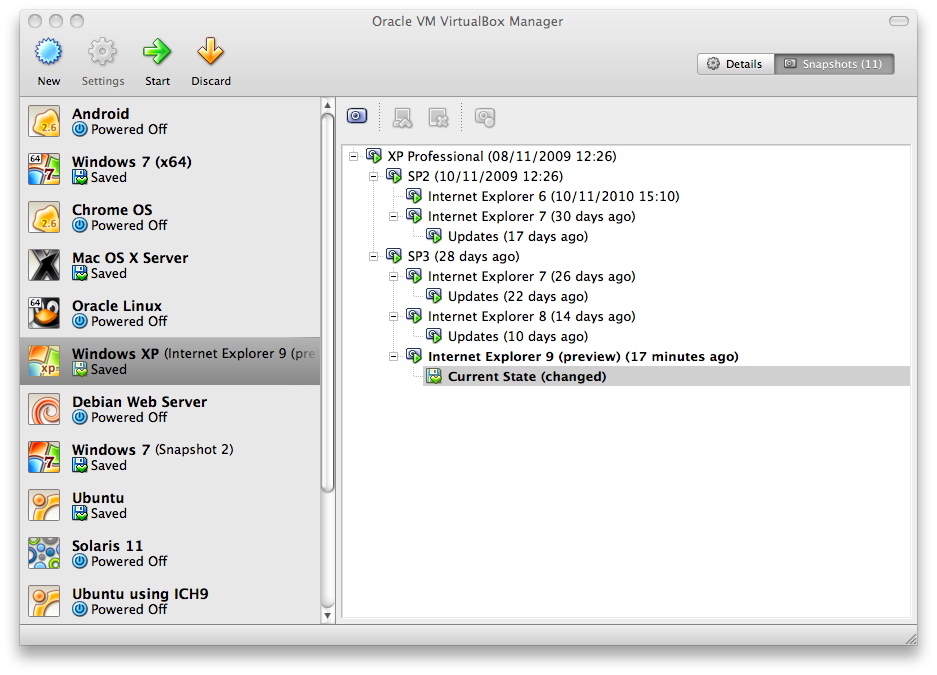
\includegraphics[width=12cm]{images/snapshots-1.png}
\end{center}

VirtualBox imposes no limits on the number of snapshots you
            can take. The only practical limitation is disk space on your
            host: each snapshot stores the state of the virtual machine and
            thus occupies some disk space. (See the next section for details
            on what exactly is stored in a snapshot.)


\item 

You can \textbf{restore a snapshot}
            by right-clicking on any snapshot you have taken in the list of
            snapshots. By restoring a snapshot, you go back (or forward) in
            time: the current state of the machine is lost, and the machine is
            restored to the exact state it was in when the snapshot was
            taken.\footnote{Both the terminology and the functionality of restoring
                snapshots has changed with VirtualBox 3.1. Before that
                version, it was only possible to go back to the very last
                snapshot taken -- not earlier ones, and the operation was
                called \OQ{}Discard current state\CQ{} instead of \OQ{}Restore last
                snapshot\CQ{}. The limitation has been lifted with version 3.1. It
                is now possible to restore \textit{any} snapshot,
                going backward and forward in time.}

\vspace{.2cm}

\begin{center}\fbox{\begin{minipage}[c]{0.9\textwidth}\color{colNote}\textbf{Note:} Restoring a snapshot will affect the virtual hard drives
              that are connected to your VM, as the entire state of the
              virtual hard drive will be reverted as well. This means also
              that all files that have been created since the snapshot and all
              other file changes \textit{will be lost. }In order
              to prevent such data loss while still making use of the snapshot
              feature, it is possible to add a second hard drive in
              \OQ{}write-through\CQ{} mode using the
              \texttt{VBoxManage} interface and use it
              to store your data. As write-through hard drives are
              \textit{not} included in snapshots, they remain
              unaltered when a machine is reverted. See chapter \ref{hdimagewrites}, \textit{\nameref{hdimagewrites}}, page \pageref{hdimagewrites} for details.\end{minipage}}\end{center}

\vspace{.2cm}



To avoid losing the current state when restoring a snapshot,
            you can create a new snapshot before the restore.

By restoring an earlier snapshot and taking more snapshots
            from there, it is even possible to create a kind of alternate
            reality and to switch between these different histories of the
            virtual machine. This can result in a whole tree of virtual
            machine snapshots, as shown in the screenshot above.


\item 

You can also \textbf{delete a
            snapshot}, which will not affect the state of the
            virtual machine, but only release the files on disk that
            VirtualBox used to store the snapshot data, thus freeing disk
            space. To delete a snapshot, right-click on it in the snapshots
            tree and select \OQ{}Delete\CQ{}. As of VirtualBox 3.2, snapshots can be
            deleted even while a machine is running.

\vspace{.2cm}

\begin{center}\fbox{\begin{minipage}[c]{0.9\textwidth}\color{colNote}\textbf{Note:} Whereas taking and restoring snapshots are fairly quick
                operations, deleting a snapshot can take a considerable amount
                of time since large amounts of data may need to be copied
                between several disk image files. Temporary disk files may
                also need large amounts of disk space while the operation is
                in progress.\end{minipage}}\end{center}

\vspace{.2cm}



There are some situations which cannot be handled while a VM
            is running, and you will get an appropriate message that you need
            to perform this snapshot deletion when the VM is shut down.

\end{enumerate}


\subsection{Snapshot contents}


Think of a snapshot as a point in time that you have preserved.
      More formally, a snapshot consists of three things:

\begin{itemize}


\item 

It contains a complete copy of the VM settings, including
            the hardware configuration, so that when you restore a snapshot,
            the VM settings are restored as well. (For example, if you changed
            the hard disk configuration or the VM's system settings, that
            change is undone when you restore the snapshot.)

The copy of the settings is stored in the machine
            configuration, an XML text file, and thus occupies very little
            space.


\item 

The complete state of all the virtual disks attached to the
            machine is preserved. Going back to a snapshot means that all
            changes that had been made to the machine's disks -- file by file,
            bit by bit -- will be undone as well. Files that were since
            created will disappear, files that were deleted will be restored,
            changes to files will be reverted.

(Strictly speaking, this is only true for virtual hard disks
            in \OQ{}normal\CQ{} mode. As mentioned above, you can configure disks to
            behave differently with snapshots; see chapter \ref{hdimagewrites}, \textit{\nameref{hdimagewrites}}, page \pageref{hdimagewrites}. Even more formally and technically
            correct, it is not the virtual disk itself that is restored when a
            snapshot is restored. Instead, when a snapshot is taken,
            VirtualBox creates differencing images which contain only the
            changes since the snapshot were taken, and when the snapshot is
            restored, VirtualBox throws away that differencing image, thus
            going back to the previous state. This is both faster and uses
            less disk space. For the details, which can be complex, please see
            chapter \ref{diffimages}, \textit{\nameref{diffimages}}, page \pageref{diffimages}.)

Creating the differencing image as such does not occupy much
            space on the host disk initially, since the differencing image
            will initially be empty (and grow dynamically later with each
            write operation to the disk). The longer you use the machine after
            having created the snapshot, however, the more the differencing
            image will grow in size.


\item 

Finally, if you took a snapshot while the machine was
            running, the memory state of the machine is also saved in the
            snapshot (the same way the memory can be saved when you close the
            VM window). When you restore such a snapshot, execution resumes at
            exactly the point when the snapshot was taken.

The memory state file can be as large as the memory size of
            the virtual machine and will therefore occupy quite some disk
            space as well.

\end{itemize}


\section{Virtual machine configuration}
\label{configbasics}


When you select a virtual machine from the list in the Manager
    window, you will see a summary of that machine's settings on the
    right.

Clicking on the \OQ{}Settings\CQ{} button in the toolbar at the top brings
    up a detailed window where you can configure many of the properties of the
    selected VM. But be careful: even though it is possible to change all VM
    settings after installing a guest operating system, certain changes might
    prevent a guest operating system from functioning correctly if done after
    installation.

\vspace{.2cm}

\begin{center}\fbox{\begin{minipage}[c]{0.9\textwidth}\color{colNote}\textbf{Note:} The \OQ{}Settings\CQ{} button is disabled while a VM is either in the
      \OQ{}running\CQ{} or \OQ{}saved\CQ{} state. This is simply because the settings dialog
      allows you to change fundamental characteristics of the virtual computer
      that is created for your guest operating system, and this operating
      system may not take it well when, for example, half of its memory is
      taken away from under its feet. As a result, if the \OQ{}Settings\CQ{} button is
      disabled, shut down the current VM first.\end{minipage}}\end{center}

\vspace{.2cm}



VirtualBox provides a plethora of parameters that can be changed for
    a virtual machine. The various settings that can be changed in the
    \OQ{}Settings\CQ{} window are described in detail in chapter \ref{BasicConcepts}, \textit{\nameref{BasicConcepts}}, page \pageref{BasicConcepts}. Even more parameters are available with the
    VirtualBox command line interface; see chapter \ref{vboxmanage}, \textit{\nameref{vboxmanage}}, page \pageref{vboxmanage}.

\section{Removing virtual machines}


To remove a virtual machine which you no longer need, right-click on
    it in the Manager's VM list select \OQ{}Remove\CQ{} from the context menu that
    comes up.

A confirmation window will come up that allows you to select whether
    the machine should only be removed from the list of machines or whether
    the files associated with it should also be deleted.

The \OQ{}Remove\CQ{} menu item is disabled while a machine is
    running.

\section{Cloning virtual machines}
\label{clone}


To experiment with a VM configuration, test different guest OS levels
    or to simply backup a VM, VirtualBox can create a full or a linked copy of
    an existing VM.\footnote{Cloning support was introduced with VirtualBox
    4.1.}

A wizard will guide you through the clone process:\begin{center}
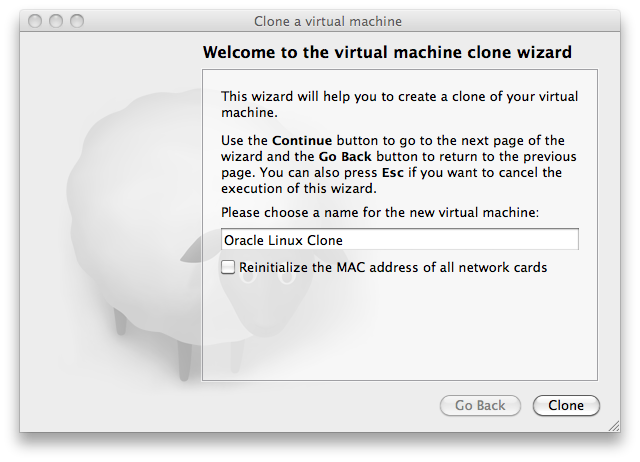
\includegraphics[width=10cm]{images/clone-vm.png}
\end{center}

This wizard can be invoked from the context menu of the Manager's VM
    list (select \OQ{}Clone\CQ{}) or the \OQ{}Snapshots\CQ{} view of the selected VM. First
    choose a new name for the clone. When you select \textbf{Reinitialize the MAC address of all network cards}
    every network card get a new MAC address assigned. This is useful when
    both, the source VM and the cloned VM, have to operate on the same network.
    If you leave this unchanged, all network cards have the same MAC address
    like the one in the source VM. Depending on how you invoke the wizard you
    have different choices for the cloning operation. First you need to decide
    if the clone should be linked to the source VM or a fully independent clone
    should be created:

\begin{itemize}


\item 

\textbf{Full clone:} In this mode all
             depending disk images are copied to the new VM folder. The clone
             can fully operate without the source VM.
         


\item 

\textbf{Linked clone:} In this mode new
             differencing disk images are created where the parent disk images
             are the source disk images. If you selected the current state of
             the source VM as clone point, a new snapshot will be created
             implicitly.
         

\end{itemize}


After selecting the clone mode, you need to decide about what exactly
    should be cloned. You can always create a clone of the \textit{current state} only or \textit{all}. When you select \textit{all}, the current state and in addition all
    snapshots are cloned. Have you started from a snapshot which has additional
    children, you can also clone the \textit{current state and
        all children}. This creates a clone starting with this
    snapshot and includes all child snaphots.

The clone operation itself can be a lengthy operation depending on
    the size and count of the attached disk images. Also keep in mind that
    every snapshot has differencing disk images attached, which need to be
    cloned as well.

The \OQ{}Clone\CQ{} menu item is disabled while a machine is running.

For how to clone a VM at the command line, please see chapter \ref{vboxmanage-clonevm}, \textit{\nameref{vboxmanage-clonevm}}, page \pageref{vboxmanage-clonevm}.

\section{Importing and exporting virtual machines}
\label{ovf}


VirtualBox can import and export virtual machines in the
    industry-standard Open Virtualization Format (OVF).\footnote{OVF support was originally introduced with VirtualBox 2.2 and
        has seen major improvements with every version since.}

OVF is a cross-platform standard supported by many virtualization
    products which allows for creating ready-made virtual machines that can
    then be imported into a virtualizer such as VirtualBox. VirtualBox makes
    OVF import and export easy to access and supports it from the Manager
    window as well as its command-line interface. This allows for packaging
    so-called \textbf{virtual appliances}: disk images
    together with configuration settings that can be distributed easily. This
    way one can offer complete ready-to-use software packages (operating
    systems with applications) that need no configuration or installation
    except for importing into VirtualBox.

\vspace{.2cm}

\begin{center}\fbox{\begin{minipage}[c]{0.9\textwidth}\color{colNote}\textbf{Note:} The OVF standard is complex, and support in VirtualBox is an
        ongoing process. In particular, no guarantee is made that VirtualBox
        supports all appliances created by other virtualization software. For
        a list of known limitations, please see chapter \ref{KnownIssues}, \textit{\nameref{KnownIssues}}, page \pageref{KnownIssues}.\end{minipage}}\end{center}

\vspace{.2cm}



Appliances in OVF format can appear in two variants:

\begin{enumerate}


\item 

They can come in several files, as one or several disk images,
          typically in the widely-used VMDK format (see chapter \ref{vdidetails}, \textit{\nameref{vdidetails}}, page \pageref{vdidetails}) and a textual description file in an XML
          dialect with an \texttt{.ovf} extension.
          These files must then reside in the same directory for VirtualBox to
          be able to import them.


\item 

Alternatively, the above files can be packed together into a
          single archive file, typically with an
          \texttt{.ova} extension. (Such archive files
          use a variant of the TAR archive format and can therefore be
          unpacked outside of VirtualBox with any utility that can unpack
          standard TAR files.)

\end{enumerate}


To \textbf{import} an appliance in one of
    the above formats, simply double-click on the OVF/OVA file.\footnote{Starting with version 4.0, VirtualBox creates file type
        associations for OVF and OVA files on your host operating
        system.} Alternatively, select \OQ{}File\CQ{} -> \OQ{}Import appliance\CQ{} from
    the Manager window. In the file dialog that comes up, navigate to the file
    with either the \texttt{.ovf} or the
    \texttt{.ova} file extension.

If VirtualBox can handle the file, a dialog similar to the following
    will appear:

\begin{center}
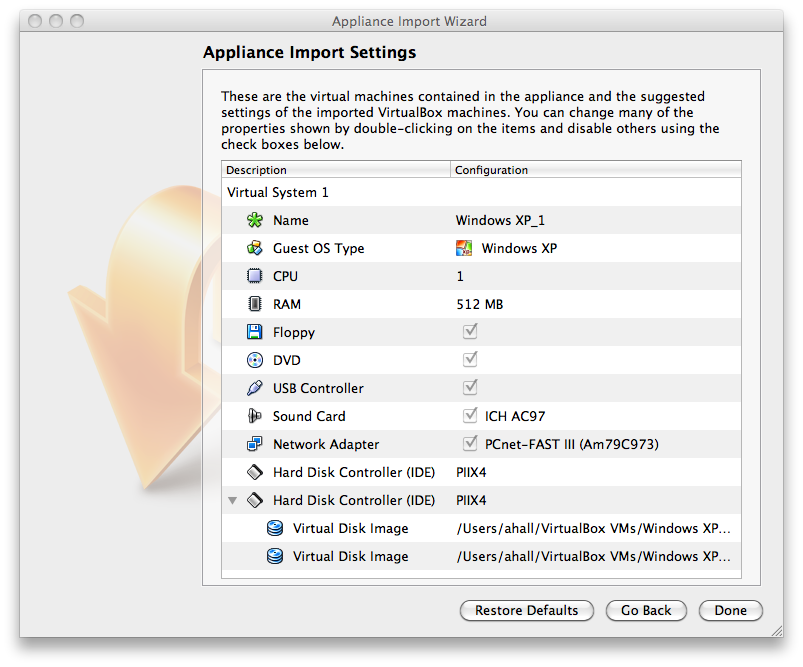
\includegraphics[width=12cm]{images/ovf-import.png}
\end{center}This presents the virtual machines described in the OVF
    file and allows you to change the virtual machine settings by
    double-clicking on the description items. Once you click on \textbf{\OQ{}Import\CQ{}}, VirtualBox will copy the disk images and
    create local virtual machines with the settings described in the dialog.
    These will then show up in the Manager's list of virtual machines.

Note that since disk images tend to be big, and VMDK images that
    come with virtual appliances are typically shipped in a special compressed
    format that is unsuitable for being used by virtual machines directly, the
    images will need to be unpacked and copied first, which can take a few
    minutes.

For how to import an image at the command line, please see chapter \ref{vboxmanage-import}, \textit{\nameref{vboxmanage-import}}, page \pageref{vboxmanage-import}.

Conversely, to \textbf{export} virtual
    machines that you already have in VirtualBox, select \OQ{}File\CQ{} -> \OQ{}Export
    appliance\CQ{}. A different dialog window shows up that allows you to combine
    several virtual machines into an OVF appliance. Then, select the target
    location where the target files should be stored, and the conversion
    process begins. This can again take a while.

For how to export an image at the command line, please see chapter \ref{vboxmanage-export}, \textit{\nameref{vboxmanage-export}}, page \pageref{vboxmanage-export}.

\vspace{.2cm}

\begin{center}\fbox{\begin{minipage}[c]{0.9\textwidth}\color{colNote}\textbf{Note:} OVF cannot describe snapshots that were taken for a virtual
        machine. As a result, when you export a virtual machine that has
        snapshots, only the current state of the machine will be exported, and
        the disk images in the export will have a \OQ{}flattened\CQ{} state identical
        to the current state of the virtual machine.\end{minipage}}\end{center}

\vspace{.2cm}



\section{Global Settings}
\label{globalsettings}


The global settings dialog can be reached through the
    \textbf{File} menu, selecting the
    \textbf{Preferences...} item. It offers a selection
    of settings which apply to all virtual machines of the current user or in
    the case of \textbf{Extensions} to the entire
    system:
    

\begin{enumerate}


\item 

\textbf{General} Enables the user to
         specify the default folder/directory for VM files, and the VRDP
         Authentication Library.


\item 

\textbf{Input} Enables the user to
         specify the Host Key. It identifies the key that toggles whether the
         cursor is in the focus of the VM or the Host operating system
         windows (see chapter \ref{keyb_mouse_normal}, \textit{\nameref{keyb_mouse_normal}}, page \pageref{keyb_mouse_normal}) and which is also
         used to trigger certain VM actions (see chapter \ref{specialcharacters}, \textit{\nameref{specialcharacters}}, page \pageref{specialcharacters})


\item 

\textbf{Update} Enables the user
         to specify various settings for Automatic Updates.


\item 

\textbf{Language} Enables the user to
         specify the GUI language.


\item 

\textbf{Display} Enables the user to
         specify the screen resolution, and its width and height.


\item 

\textbf{Network} Enables the user to
         configure the details of Host Only Networks.


\item 

\textbf{Extensions} Enables the user
         to list and manage the installed extension packages.


\item 

\textbf{Proxy} Enables the user to
         configure a HTTP Proxy Server.

\end{enumerate}


\section{Alternative front-ends}
\label{frontends}


As briefly mentioned in chapter \ref{features-overview}, \textit{\nameref{features-overview}}, page \pageref{features-overview},
    VirtualBox has a very flexible internal design that allows for using
    multiple interfaces to control the same virtual machines. To illustrate,
    you can, for example, start a virtual machine with the VirtualBox Manager
    window and then stop it from the command line. With VirtualBox's support
    for the Remote Desktop Protocol (RDP), you can even run virtual machines
    remotely on a headless server and have all the graphical output redirected
    over the network.

In detail, the following front-ends are shipped in the standard
    VirtualBox package:



\begin{enumerate}


\item 

\texttt{VirtualBox} is the VirtualBox
          Manager. This graphical user interface uses the Qt toolkit; most of
          this User Manual is dedicated to describing it. While this is the
          easiest to use, some of the more advanced VirtualBox features are
          kept away from it to keep it simple.


\item 

\texttt{VBoxManage} is our
          command-line interface for automated and very detailed control of
          every aspect of VirtualBox. It is described in chapter \ref{vboxmanage}, \textit{\nameref{vboxmanage}}, page \pageref{vboxmanage}.


\item 

\texttt{VBoxSDL} is an alternative,
          simple graphical front-end with an intentionally limited feature
          set, designed to only display virtual machines that are controlled
          in detail with \texttt{VBoxManage}. This is
          interesting for business environments where displaying all the bells
          and whistles of the full GUI is not feasible.
          \texttt{VBoxSDL} is described in chapter \ref{vboxsdl}, \textit{\nameref{vboxsdl}}, page \pageref{vboxsdl}.


\item 

Finally, \texttt{VBoxHeadless} is yet
          another front-end that produces no visible output on the host at
          all, but merely acts as a RDP server if the VirtualBox Remote
          Desktop Extension (VRDE) is installed. As opposed to the other
          graphical interfaces, the headless front-end requires no graphics
          support. This is useful, for example, if you want to host your
          virtual machines on a headless Linux server that has no X Window
          system installed. For details, see chapter \ref{vboxheadless}, \textit{\nameref{vboxheadless}}, page \pageref{vboxheadless}.

\end{enumerate}
If the above front-ends still do not satisfy your
    particular needs, it is possible to create yet another front-end to the
    complex virtualization engine that is the core of VirtualBox, as the
    VirtualBox core neatly exposes all of its features in a clean API; please
    refer to chapter \ref{VirtualBoxAPI}, \textit{\nameref{VirtualBoxAPI}}, page \pageref{VirtualBoxAPI}.

\chapter{Installation details}
\label{installation}


As installation of VirtualBox varies depending on your host operating
  system, we provide installation instructions in four separate chapters for
  Windows, Mac OS X, Linux and Solaris, respectively.

\section{Installing on Windows hosts}
\label{installation_windows}


\subsection{Prerequisites}


For the various versions of Windows that we support as host
      operating systems, please refer to chapter \ref{hostossupport}, \textit{\nameref{hostossupport}}, page \pageref{hostossupport}.

In addition, Windows Installer 1.1 or higher must be present on
      your system. This should be the case if you have all recent Windows
      updates installed.

\subsection{Performing the installation}


The VirtualBox installation can be started 

\begin{itemize}


\item 

either by double-clicking on its executable file (contains
            both 32- and 64-bit architectures)


\item 

or by entering 

\begin{Verbatim}[fontsize=\footnotesize]
VirtualBox.exe -extract
\end{Verbatim}


on the command line. This will extract both installers into
            a temporary directory in which you'll then find the usual .MSI
            files. Then you can do a 

\begin{Verbatim}[fontsize=\footnotesize]
msiexec /i VirtualBox-<version>-MultiArch_<x86|amd64>.msi
\end{Verbatim}

            to perform the installation.

\end{itemize}


In either case, this will display the installation welcome dialog
      and allow you to choose where to install VirtualBox to and which
      components to install. In addition to the VirtualBox application, the
      following components are available:

\begin{description}


\item[USB support]

This package contains special drivers for your Windows
              host that VirtualBox requires to fully support USB devices
              inside your virtual machines.

\item[Networking]

This package contains extra networking drivers for your
              Windows host that VirtualBox needs to support Bridged Networking
              (to make your VM's virtual network cards accessible from other
              machines on your physical network).

\item[Python Support]

This package contains Python scripting support for the
              VirtualBox API (see chapter \ref{VirtualBoxAPI}, \textit{\nameref{VirtualBoxAPI}}, page \pageref{VirtualBoxAPI}). For this
              to work, an already working Windows Python installation on the
              system is required.\footnote{See, for example, \url{http://www.python.org/download/windows/}.}
\end{description}


Depending on your Windows configuration, you may see warnings
      about \OQ{}unsigned drivers\CQ{} or similar. Please select \OQ{}Continue\CQ{} on these
      warnings as otherwise VirtualBox might not function correctly after
      installation.

The installer will create a \OQ{}VirtualBox\CQ{} group in the Windows
      \OQ{}Start\CQ{} menu which allows you to launch the application and access its
      documentation.

With standard settings, VirtualBox will be installed for all users
      on the local system. In case this is not wanted, you have to invoke the
      installer by first extracting it by using 

\begin{Verbatim}[fontsize=\footnotesize]
VirtualBox.exe -extract
\end{Verbatim}

      and then do as follows: 

\begin{Verbatim}[fontsize=\footnotesize]
VirtualBox.exe -msiparams ALLUSERS=2
\end{Verbatim}

      or 

\begin{Verbatim}[fontsize=\footnotesize]
msiexec /i VirtualBox-<version>-MultiArch_<x86|amd64>.msi ALLUSERS=2
\end{Verbatim}

      on the extracted .MSI files. This will install VirtualBox only for the
      current user.

If you do not want to install all features of VirtualBox, you can
      set the optional \texttt{ADDLOCAL} parameter to
      explicitly name the features to be installed. The following features are
      available: 

\begin{description}


\item[VBoxApplication]

Main binaries of VirtualBox.

\vspace{.2cm}

\begin{center}\fbox{\begin{minipage}[c]{0.9\textwidth}\color{colNote}\textbf{Note:} This feature must not be absent since it contains the
                  minimum set of files to have working VirtualBox
                  installation.\end{minipage}}\end{center}

\vspace{.2cm}



\item[VBoxUSB]

USB support.

\item[VBoxNetwork]

All networking support; includes the VBoxNetworkFlt and
              VBoxNetworkAdp features (see below).

\item[VBoxNetworkFlt]

Bridged networking support.

\item[VBoxNetworkAdp]

Host-only networking support.

\item[VBoxPython]

Python support.
\end{description}
For example, to only install USB support along with the
      main binaries, do a: 

\begin{Verbatim}[fontsize=\footnotesize]
VirtualBox.exe -msiparams ADDLOCAL=VBoxApplication,VBoxUSB
\end{Verbatim}

      or 

\begin{Verbatim}[fontsize=\footnotesize]
msiexec /i VirtualBox-<version>-MultiArch_<x86|amd64>.msi ADDLOCAL=VBoxApplication,VBoxUSB
\end{Verbatim}


\subsection{Uninstallation}


As VirtualBox uses the standard Microsoft Windows installer,
      VirtualBox can be safely uninstalled at any time by choosing the program
      entry in the \OQ{}Add/Remove Programs\CQ{} applet in the Windows Control
      Panel.

\subsection{Unattended installation}


Unattended installations can be performed using the standard MSI
      support.

\section{Installing on Mac OS X hosts}


\subsection{Performing the installation}


For Mac OS X hosts, VirtualBox ships in a disk image
      (\texttt{dmg}) file. Perform the following
      steps: 

\begin{enumerate}


\item 

Double-click on that file to have its contents
            mounted.


\item 

A window will open telling you to double click on the
            \texttt{VirtualBox.mpkg} installer file
            displayed in that window.


\item 

This will start the installer, which will allow you to
            select where to install VirtualBox to.

\end{enumerate}


After installation, you can find a VirtualBox icon in the
      \OQ{}Applications\CQ{} folder in the Finder.

\subsection{Uninstallation}


To uninstall VirtualBox, open the disk image (dmg) file again and
      double-click on the uninstall icon contained therein.

\subsection{Unattended installation}


To perform a non-interactive installation of VirtualBox you can
      use the command line version of the installer application.

Mount the disk image (dmg) file as described in the normal
      installation or use the following command line:

\begin{Verbatim}[fontsize=\footnotesize]
hdiutil attach /path/to/VirtualBox-xyz.dmg
\end{Verbatim}


Then open a terminal session and execute:

\begin{Verbatim}[fontsize=\footnotesize]
sudo installer -pkg /Volumes/VirtualBox/VirtualBox.pkg -target /Volumes/Macintosh\ HD
\end{Verbatim}


\section{Installing on Linux hosts}
\label{install-linux-host}


\subsection{Prerequisites}


For the various versions of Linux that we support as host
      operating systems, please refer to chapter \ref{hostossupport}, \textit{\nameref{hostossupport}}, page \pageref{hostossupport}.

You will need to install the following packages on your Linux
      system before starting the installation (some systems will do this for
      you automatically when you install VirtualBox):

\begin{itemize}


\item 

Qt 4.6.2 or higher;


\item 

SDL 1.2.7 or higher (this graphics library is typically called
          \texttt{libsdl} or similar).

\end{itemize}


\vspace{.2cm}

\begin{center}\fbox{\begin{minipage}[c]{0.9\textwidth}\color{colNote}\textbf{Note:} To be precise, these packages are only required if you want to
        run the VirtualBox graphical user interfaces. In particular,
        \texttt{VirtualBox}, the graphical VirtualBox
        manager, requires both Qt and SDL;
        \texttt{VBoxSDL}, our simplified GUI, requires
        only SDL. By contrast, if you only want to run
        \texttt{VBoxHeadless}, neither Qt nor SDL are
        required.\end{minipage}}\end{center}

\vspace{.2cm}



\subsection{The VirtualBox kernel module}
\label{externalkernelmodules}


VirtualBox uses a special kernel module called
      \texttt{vboxdrv} to perform physical memory
      allocation and to gain control of the processor for guest system
      execution. Without this kernel module, you can still use the VirtualBox
      manager to configure virtual machines, but they will not start. In
      addition, there are the network kernel modules
      \texttt{vboxnetflt} and
      \texttt{vboxnetadp} which are required for the
      more advanced networking features of VirtualBox.

The VirtualBox kernel module is automatically installed on your
      system when you install VirtualBox. To maintain it with future kernel
      updates, for those Linux distributions which provide it -- most current
      ones -- we recommend installing Dynamic Kernel Module Support
      (DKMS)\footnote{See \url{http://en.wikipedia.org/wiki/Dynamic\_Kernel\_Module\_Support}
          for an introduction.}. This framework helps with building and upgrading kernel
      modules.

If DKMS is not already installed, execute one of the following:
      

\begin{itemize}


\item 

On an Ubuntu system:

\begin{Verbatim}[fontsize=\footnotesize]
sudo apt-get install dkms
\end{Verbatim}



\item 

On a Fedora system:

\begin{Verbatim}[fontsize=\footnotesize]
yum install dkms
\end{Verbatim}



\item 

On a Mandriva or Mageia system:

\begin{Verbatim}[fontsize=\footnotesize]
urpmi dkms
\end{Verbatim}


\end{itemize}


If DKMS is available and installed, the VirtualBox kernel module
      should always work automatically, and it will be automatically rebuilt
      if your host kernel is updated.

Otherwise, there are only two situations in which you will need to
      worry about the kernel module:

\begin{enumerate}


\item 

The original installation fails. This probably means that
            your Linux system is not prepared for building external kernel
            modules.

Most Linux distributions can be set up simply by installing
            the right packages - normally, these will be the GNU compiler
            (GCC), GNU Make (make) and packages containing header files for
            your kernel - and making sure that all system updates are
            installed and that the system is running the most up-to-date
            kernel included in the distribution. \textit{The version numbers
            of the header file packages must be the same as that of the kernel
            you are using.}

\begin{itemize}


\item 

With Debian and Ubuntu releases, you must install the
                right version of the
                \texttt{linux-headers} and if it
                exists the \texttt{linux-kbuild}
                package. Current Ubuntu releases should have the right
                packages installed by default.


\item 

In even older Debian and Ubuntu releases, you must
                install the right version of the
                \texttt{kernel-headers}
                package.


\item 

On Fedora and Redhat systems, the package is
                \texttt{kernel-devel}.


\item 

On SUSE and openSUSE Linux, you must install the right
                versions of the \texttt{kernel-source}
                and \texttt{kernel-syms}
                packages.


\item 

If you have built your own kernel, you will need to make
                sure that you also installed all the required header and other
                files for building external modules to the right locations.
                The details of how to do this will depend on how you built
                your kernel, and if you are unsure you should consult the
                documentation which you followed to do so.

\end{itemize}



\item 

The kernel of your Linux host was updated and DKMS is not
            installed. In that case, the kernel module will need to be
            reinstalled by executing (as root):

\begin{Verbatim}[fontsize=\footnotesize]
/etc/init.d/vboxdrv setup
\end{Verbatim}


\end{enumerate}


\subsection{Performing the installation}


VirtualBox is available in a number of package formats native to
      various common Linux distributions (see chapter \ref{hostossupport}, \textit{\nameref{hostossupport}}, page \pageref{hostossupport}
      for details). In addition, there is an alternative generic installer
      (.run) which should work on most Linux distributions.

\subsubsection{Installing VirtualBox from a Debian/Ubuntu package}


First, download the appropriate package for your distribution.
        The following examples assume that you are installing to a 32-bit
        Ubuntu Raring system. Use \texttt{dpkg} to
        install the Debian package:

\begin{Verbatim}[fontsize=\footnotesize]
sudo dpkg -i VirtualBox-3.2_4.3.28_OSE_Ubuntu_raring_i386.deb
\end{Verbatim}


You will be asked to accept the VirtualBox Personal Use and
        Evaluation License. Unless you answer \OQ{}yes\CQ{} here, the installation
        will be aborted.

The installer will also search for a VirtualBox kernel module
        suitable for your kernel. The package includes pre-compiled modules
        for the most common kernel configurations. If no suitable kernel
        module is found, the installation script tries to build a module
        itself. If the build process is not successful you will be shown a
        warning and the package will be left unconfigured. Please have a look
        at \texttt{/var/log/vbox-install.log} to find
        out why the compilation failed. You may have to install the
        appropriate Linux kernel headers (see chapter \ref{externalkernelmodules}, \textit{\nameref{externalkernelmodules}}, page \pageref{externalkernelmodules}). After correcting any problems, do
        

\begin{Verbatim}[fontsize=\footnotesize]
sudo /etc/init.d/vboxdrv setup
\end{Verbatim}
This will start a
        second attempt to build the module.

If a suitable kernel module was found in the package or the
        module was successfully built, the installation script will attempt to
        load that module. If this fails, please see chapter \ref{ts_linux-kernelmodule-fails-to-load}, \textit{\nameref{ts_linux-kernelmodule-fails-to-load}}, page \pageref{ts_linux-kernelmodule-fails-to-load} for further
        information.

Once VirtualBox has been successfully installed and configured,
        you can start it by selecting \OQ{}VirtualBox\CQ{} in your start menu or from
        the command line (see chapter \ref{startingvboxonlinux}, \textit{\nameref{startingvboxonlinux}}, page \pageref{startingvboxonlinux}).

\subsubsection{Using the alternative installer (VirtualBox.run)}


The alternative installer performs the following steps:

\begin{itemize}


\item 

It unpacks the application files to the target directory,
            

\begin{Verbatim}[fontsize=\footnotesize]
/opt/VirtualBox/
\end{Verbatim}
 which cannot be changed.


\item 

It builds the VirtualBox kernel modules
            (\texttt{vboxdrv},
            \texttt{vboxnetflt} and
            \texttt{vboxnetadp}) and installs
            them.


\item 

It creates
            \texttt{/etc/init.d/vboxdrv}, an init
            script to start the VirtualBox kernel module.


\item 

It creates a new system group called
            \texttt{vboxusers}.


\item 

It creates symbolic links in
            \texttt{/usr/bin} to the a shell script
            (\texttt{/opt/VirtualBox/VBox}) which does
            some sanity checks and dispatches to the actual executables,
            \texttt{VirtualBox},
            \texttt{VBoxSDL},
            \texttt{VBoxVRDP},
            \texttt{VBoxHeadless} and
            \texttt{VBoxManage}


\item 

It creates
            \texttt{/etc/udev/rules.d/60-vboxdrv.rules},
            a description file for udev, if that is present, which makes the
            USB devices accessible to all users in the
            \texttt{vboxusers} group.


\item 

It writes the installation directory to
            \texttt{/etc/vbox/vbox.cfg}.

\end{itemize}


The installer must be executed as root with either
        \texttt{install} or
        \texttt{uninstall} as the first
        parameter.

\begin{Verbatim}[fontsize=\footnotesize]
sudo ./VirtualBox.run install
\end{Verbatim}


Or if you do not have the \OQ{}sudo\CQ{} command available, run the
        following as root instead:

\begin{Verbatim}[fontsize=\footnotesize]
./VirtualBox.run install
\end{Verbatim}


After that you need to put every user which should be able to
        access USB devices from VirtualBox guests in the group
        \texttt{vboxusers}, either through the GUI
        user management tools or by running the following command as
        root:

\begin{Verbatim}[fontsize=\footnotesize]
sudo usermod -a -G vboxusers username
\end{Verbatim}




\vspace{.2cm}

\begin{center}\fbox{\begin{minipage}[c]{0.9\textwidth}\color{colNote}\textbf{Note:} The \texttt{usermod} command of some
            older Linux distributions does not support the
            \texttt{-a} option (which adds the user to
            the given group without affecting membership of other groups). In
            this case, find out the current group memberships with the
            \texttt{groups} command and add all these
            groups in a comma-separated list to the command line after the
            \texttt{-G} option, e.g. like this:
            \texttt{usermod -G group1,group2,vboxusers
            username}.\end{minipage}}\end{center}

\vspace{.2cm}



\subsubsection{Performing a manual installation}


If, for any reason, you cannot use the shell script installer
        described previously, you can also perform a manual installation.
        Invoke the installer like this:

\begin{Verbatim}[fontsize=\footnotesize]
./VirtualBox.run --keep --noexec
\end{Verbatim}


This will unpack all the files needed for installation in the
        directory \texttt{install} under the current
        directory. The VirtualBox application files are contained in
        \texttt{VirtualBox.tar.bz2} which you can
        unpack to any directory on your system. For example:

\begin{Verbatim}[fontsize=\footnotesize]
sudo mkdir /opt/VirtualBox
sudo tar jxf ./install/VirtualBox.tar.bz2 -C /opt/VirtualBox
\end{Verbatim}


or as root:

\begin{Verbatim}[fontsize=\footnotesize]
mkdir /opt/VirtualBox
tar jxf ./install/VirtualBox.tar.bz2 -C /opt/VirtualBox
\end{Verbatim}


The sources for VirtualBox's kernel module are provided in the
        \texttt{src} directory. To build the module,
        change to the directory and issue

\begin{Verbatim}[fontsize=\footnotesize]
make
\end{Verbatim}


If everything builds correctly, issue the following command to
        install the module to the appropriate module directory:

\begin{Verbatim}[fontsize=\footnotesize]
sudo make install
\end{Verbatim}


In case you do not have sudo, switch the user account to root
        and perform

\begin{Verbatim}[fontsize=\footnotesize]
make install
\end{Verbatim}


The VirtualBox kernel module needs a device node to operate. The
        above make command will tell you how to create the device node,
        depending on your Linux system. The procedure is slightly different
        for a classical Linux setup with a
        \texttt{/dev} directory, a system with the now
        deprecated \texttt{devfs} and a modern Linux
        system with \texttt{udev}.

On certain Linux distributions, you might experience
        difficulties building the module. You will have to analyze the error
        messages from the build system to diagnose the cause of the problems.
        In general, make sure that the correct Linux kernel sources are used
        for the build process.

Note that the \texttt{/dev/vboxdrv}
        kernel module device node must be owned by root:root and must be
        read/writable only for the user.

Next, you will have to install the system initialization script
        for the kernel module:

\begin{Verbatim}[fontsize=\footnotesize]
cp /opt/VirtualBox/vboxdrv.sh /etc/init.d/vboxdrv
\end{Verbatim}
(assuming
        you installed VirtualBox to the
        \texttt{/opt/VirtualBox} directory) and
        activate the initialization script using the right method for your
        distribution. You should create VirtualBox's configuration
        file:

\begin{Verbatim}[fontsize=\footnotesize]
mkdir /etc/vbox
echo INSTALL_DIR=/opt/VirtualBox > /etc/vbox/vbox.cfg
\end{Verbatim}
and, for
        convenience, create the following symbolic links:

\begin{Verbatim}[fontsize=\footnotesize]
ln -sf /opt/VirtualBox/VBox.sh /usr/bin/VirtualBox
ln -sf /opt/VirtualBox/VBox.sh /usr/bin/VBoxManage
ln -sf /opt/VirtualBox/VBox.sh /usr/bin/VBoxHeadless
ln -sf /opt/VirtualBox/VBox.sh /usr/bin/VBoxSDL
\end{Verbatim}


\subsubsection{Updating and uninstalling VirtualBox}


Before updating or uninstalling VirtualBox, you must terminate
        any virtual machines which are currently running and exit the
        VirtualBox or VBoxSVC applications. To update VirtualBox, simply run
        the installer of the updated version. To uninstall VirtualBox, invoke
        the installer like this: 

\begin{Verbatim}[fontsize=\footnotesize]
sudo ./VirtualBox.run uninstall
\end{Verbatim}

        or as root

\begin{Verbatim}[fontsize=\footnotesize]
./VirtualBox.run uninstall
\end{Verbatim}
. Starting with
        version 2.2.2, you can uninstall the .run package by invoking 

\begin{Verbatim}[fontsize=\footnotesize]
/opt/VirtualBox/uninstall.sh
\end{Verbatim}
To
        manually uninstall VirtualBox, simply undo the steps in the manual
        installation in reverse order.

\subsubsection{Automatic installation of Debian packages}


The Debian packages will request some user feedback when
        installed for the first time. The debconf system is used to perform
        this task. To prevent any user interaction during installation,
        default values can be defined. A file
        \texttt{vboxconf} can contain the following
        debconf settings: 

\begin{Verbatim}[fontsize=\footnotesize]
virtualbox virtualbox/module-compilation-allowed boolean true
virtualbox virtualbox/delete-old-modules boolean true
\end{Verbatim}
The first line
        allows compilation of the vboxdrv kernel module if no module was found
        for the current kernel. The second line allows the package to delete
        any old vboxdrv kernel modules compiled by previous
        installations.

These default settings can be applied with 

\begin{Verbatim}[fontsize=\footnotesize]
debconf-set-selections vboxconf
\end{Verbatim}

        prior to the installation of the VirtualBox Debian package.

In addition there are some common configuration options that can
        be set prior to the installation, described in chapter \ref{linux_install_opts}, \textit{\nameref{linux_install_opts}}, page \pageref{linux_install_opts}.

\subsubsection{Automatic installation of .rpm packages}


The .rpm format does not provide a configuration system
        comparable to the debconf system. See chapter \ref{linux_install_opts}, \textit{\nameref{linux_install_opts}}, page \pageref{linux_install_opts} for how to set some common
        installation options provided by VirtualBox.

\subsubsection{Automatic installation options}
\label{linux_install_opts}


To configure the installation process of our .deb and .rpm
        packages, you can create a response file named
        \texttt{/etc/default/virtualbox}. The
        automatic generation of the udev rule can be prevented by the
        following setting: 

\begin{Verbatim}[fontsize=\footnotesize]
INSTALL_NO_UDEV=1
\end{Verbatim}
 The creation of
        the group vboxusers can be prevented by 

\begin{Verbatim}[fontsize=\footnotesize]
INSTALL_NO_GROUP=1
\end{Verbatim}

        If the line 

\begin{Verbatim}[fontsize=\footnotesize]
INSTALL_NO_VBOXDRV=1
\end{Verbatim}
 is specified, the
        package installer will not try to build the
        \texttt{vboxdrv} kernel module if no module
        fitting the current kernel was found.

\subsection{The vboxusers group}


The Linux installers create the system user group
      \texttt{vboxusers} during installation. Any
      system user who is going to use USB devices from VirtualBox guests must
      be a member of that group. A user can be made a member of the group
      \texttt{vboxusers} through the GUI user/group
      management or at the command line with

\begin{Verbatim}[fontsize=\footnotesize]
sudo usermod -a -G vboxusers username
\end{Verbatim}


\subsection{Starting VirtualBox on Linux}
\label{startingvboxonlinux}


The easiest way to start a VirtualBox program is by running the
      program of your choice (\texttt{VirtualBox},
      \texttt{VBoxManage},
      \texttt{VBoxSDL} or
      \texttt{VBoxHeadless}) from a terminal. These
      are symbolic links to \texttt{VBox.sh} that
      start the required program for you.

The following detailed instructions should only be of interest if
      you wish to execute VirtualBox without installing it first. You should
      start by compiling the \texttt{vboxdrv} kernel
      module (see above) and inserting it into the Linux kernel. VirtualBox
      consists of a service daemon (\texttt{VBoxSVC})
      and several application programs. The daemon is automatically started if
      necessary. All VirtualBox applications will communicate with the daemon
      through Unix local domain sockets. There can be multiple daemon
      instances under different user accounts and applications can only
      communicate with the daemon running under the user account as the
      application. The local domain socket resides in a subdirectory of your
      system's directory for temporary files called
      \texttt{.vbox-<username>-ipc}. In case of
      communication problems or server startup problems, you may try to remove
      this directory.

All VirtualBox applications
      (\texttt{VirtualBox},
      \texttt{VBoxSDL},
      \texttt{VBoxManage} and
      \texttt{VBoxHeadless}) require the VirtualBox
      directory to be in the library path:

\begin{Verbatim}[fontsize=\footnotesize]
LD_LIBRARY_PATH=. ./VBoxManage showvminfo "Windows XP"
\end{Verbatim}


\section{Installing on Solaris hosts}
\label{install-solaris-host}


For the specific versions of Solaris that we support as host
    operating systems, please refer to chapter \ref{hostossupport}, \textit{\nameref{hostossupport}}, page \pageref{hostossupport}.

If you have a previously installed instance of VirtualBox on your
    Solaris host, please uninstall it first before installing a new instance.
    Refer to chapter \ref{uninstall-solaris-host}, \textit{\nameref{uninstall-solaris-host}}, page \pageref{uninstall-solaris-host} for uninstall
    instructions.

\subsection{Performing the installation}


VirtualBox is available as a standard Solaris package. Download
      the VirtualBox SunOS package which includes the 64-bit
      versions of VirtualBox. \textit{The installation must be performed as
      root and from the global zone} as the VirtualBox installer
      loads kernel drivers which cannot be done from non-global zones. To
      verify which zone you are currently in, execute the
      \texttt{zonename} command. Execute the following
      commands:

\begin{Verbatim}[fontsize=\footnotesize]
gunzip -cd VirtualBox-4.3.28_OSE-SunOS.tar.gz | tar xvf -
\end{Verbatim}


Starting with VirtualBox 3.1 the VirtualBox kernel package is no
      longer a separate package and has been integrated into the main package.
      Install the VirtualBox package using:

\begin{Verbatim}[fontsize=\footnotesize]
pkgadd -d VirtualBox-4.3.28_OSE-SunOS.pkg
\end{Verbatim}


\vspace{.2cm}

\begin{center}\fbox{\begin{minipage}[c]{0.9\textwidth}\color{colNote}\textbf{Note:} If you are using Solaris Zones, to install VirtualBox only into
        the current zone and not into any other zone, use
        \texttt{pkgadd -G}. For more information refer
        to the \texttt{pkgadd} manual; see also chapter \ref{solaris-zones}, \textit{\nameref{solaris-zones}}, page \pageref{solaris-zones}.\end{minipage}}\end{center}

\vspace{.2cm}



The installer will then prompt you to enter the package you wish
      to install. Choose \OQ{}1\CQ{} or \OQ{}all\CQ{} and proceed. Next the installer will ask
      you if you want to allow the postinstall script to be executed. Choose
      \OQ{}y\CQ{} and proceed as it is essential to execute this script which installs
      the VirtualBox kernel module. Following this confirmation the installer
      will install VirtualBox and execute the postinstall setup script.

Once the postinstall script has been executed your installation is
      now complete. You may now safely delete the uncompressed package and
      \texttt{autoresponse} files from your system.
      VirtualBox would be installed in
      \texttt{/opt/VirtualBox}.

\subsection{The vboxuser group}


Starting with VirtualBox 4.1, the installer creates the system
      user group \texttt{vboxuser} during installation
      for Solaris hosts that support the USB features required by VirtualBox.
      Any system user who is going to use USB devices from VirtualBox guests
      must be a member of this group. A user can be made a member of this
      group through the GUI user/group management or at the command line by
      executing as root:

\begin{Verbatim}[fontsize=\footnotesize]
usermod -G vboxuser username
\end{Verbatim}


Note that adding an active user to that group will require that
      user to log out and back in again. This should be done manually after
      successful installation of the package.

\subsection{Starting VirtualBox on Solaris}


The easiest way to start a VirtualBox program is by running the
      program of your choice (\texttt{VirtualBox},
      \texttt{VBoxManage},
      \texttt{VBoxSDL} or
      \texttt{VBoxHeadless}) from a terminal. These
      are symbolic links to \texttt{VBox.sh} that
      start the required program for you.

Alternatively, you can directly invoke the required programs from
      \texttt{/opt/VirtualBox}. Using the links
      provided is easier as you do not have to type the full path.

You can configure some elements of the
      \texttt{VirtualBox} Qt GUI such as fonts and
      colours by executing \texttt{VBoxQtconfig} from
      the terminal.

\subsection{Uninstallation}
\label{uninstall-solaris-host}


Uninstallation of VirtualBox on Solaris requires root permissions.
      To perform the uninstallation, start a root terminal session and
      execute:

\begin{Verbatim}[fontsize=\footnotesize]
pkgrm SUNWvbox
\end{Verbatim}


After confirmation, this will remove VirtualBox from your
      system.

If you are uninstalling VirtualBox version 3.0 or lower, you need
      to remove the VirtualBox kernel interface package, execute:



\begin{Verbatim}[fontsize=\footnotesize]
pkgrm SUNWvboxkern
\end{Verbatim}


\subsection{Unattended installation}


To perform a non-interactive installation of VirtualBox we have
      provided a response file named
      \texttt{autoresponse} that the installer will
      use for responses to inputs rather than ask them from you.

Extract the tar.gz package as described in the normal
      installation. Then open a root terminal session and execute:

\begin{Verbatim}[fontsize=\footnotesize]
pkgadd -d VirtualBox-4.3.28_OSE-SunOS-x86 -n -a autoresponse SUNWvbox
\end{Verbatim}


To perform a non-interactive uninstallation, open a root terminal
      session and execute:

\begin{Verbatim}[fontsize=\footnotesize]
pkgrm -n -a /opt/VirtualBox/autoresponse SUNWvbox
\end{Verbatim}


\subsection{Configuring a zone for running VirtualBox}
\label{solaris-zones}


Starting with VirtualBox 1.6 it is possible to run VirtualBox from
      within Solaris zones. For an introduction of Solaris zones, please refer
      to \url{http://www.sun.com/bigadmin/features/articles/solaris\_zones.jsp}.

Assuming that VirtualBox has already been installed into your
      zone, you need to give the zone access to VirtualBox's device node. This
      is done by performing the following steps. Start a root terminal and
      execute:

\begin{Verbatim}[fontsize=\footnotesize]
zonecfg -z vboxzone
\end{Verbatim}


Inside the \texttt{zonecfg} prompt add the
      \texttt{device} resource and
      \texttt{match} properties to the zone. Here's
      how it can be done:

\begin{Verbatim}[fontsize=\footnotesize]
zonecfg:vboxzone>add device
zonecfg:vboxzone:device>set match=/dev/vboxdrv
zonecfg:vboxzone:device>end
zonecfg:vboxzone>verify
zonecfg:vboxzone>exit
\end{Verbatim}


If you are running VirtualBox 2.2.0 or above on Solaris 11 or
      Nevada hosts, you should add a device for
      \texttt{/dev/vboxusbmon} too, similar to what
      was shown above. This does not apply to Solaris 10 hosts due to lack of
      USB support.

Replace \OQ{}vboxzone\CQ{} with the name of the zone in which you intend
      to run VirtualBox. Next reboot the zone using
      \texttt{zoneadm} and you should be able to run
      VirtualBox from within the configured zone.

\chapter{Configuring virtual machines}
\label{BasicConcepts}


Whereas chapter \ref{Introduction}, \textit{\nameref{Introduction}}, page \pageref{Introduction} gave you a quick introduction
  to VirtualBox and how to get your first virtual machine running, the
  following chapter describes in detail how to configure virtual
  machines.

You have considerable latitude in deciding what virtual hardware will
  be provided to the guest. The virtual hardware can be used for communicating
  with the host system or with other guests. For instance, if you provide
  VirtualBox with the image of a CD-ROM in an ISO file, VirtualBox can present
  this image to a guest system as if it were a physical CD-ROM. Similarly, you
  can give a guest system access to the real network via its virtual network
  card, and, if you so choose, give the host system, other guests, or
  computers on the Internet access to the guest system.

\section{Supported guest operating systems}
\label{guestossupport}


Since VirtualBox is designed to provide a generic virtualization
    environment for x86 systems, it may run operating systems of any kind,
    even those not listed here. However, the focus is to optimize VirtualBox
    for the following guest systems:



\begin{description}


\item[Windows NT 4.0]

All versions, editions and service packs are fully
            supported; however, there are some issues with older service
            packs. We recommend to install service pack 6a. Guest Additions
            are available with a limited feature set.

\item[Windows 2000 / XP / Server 2003 / Vista / Server 2008 /
            Windows 7 / Windows 8 / Server 2012]

All versions, editions and service packs are fully supported
            (including 64-bit versions, under the preconditions listed below).
            Guest Additions are available.

\item[DOS / Windows 3.x / 95 / 98 / ME]

Limited testing has been performed. Use beyond legacy
            installation mechanisms not recommended. No Guest Additions
            available.

\item[Linux 2.4]

Limited support.

\item[Linux 2.6]

All versions/editions are fully supported (32 bits and 64
            bits). Guest Additions are available.

We strongly recommend using a Linux kernel version 2.6.13 or
            higher for better performance.

\vspace{.2cm}

\begin{center}\fbox{\begin{minipage}[c]{0.9\textwidth}\color{colNote}\textbf{Note:} Certain Linux kernel releases have bugs that prevent
                them from executing in a virtual environment; please see chapter \ref{ts_linux-buggy}, \textit{\nameref{ts_linux-buggy}}, page \pageref{ts_linux-buggy} for details.\end{minipage}}\end{center}

\vspace{.2cm}



\item[Linux 3.x]

All versions/editions are fully supported (32 bits and 64
            bits). Guest Additions are available.

\item[Solaris 10 (u6 and higher), Solaris 11 (including Solaris
          11 Express)]

Fully supported (32 bits and 64 bits). Guest Additions are
            available.

\item[FreeBSD]

Requires hardware virtualization to be enabled. Limited
            support. Guest Additions are not available yet.

\item[OpenBSD]

Requires hardware virtualization to be enabled. Versions 3.7
            and later are supported. Guest Additions are not available
            yet.

\item[OS/2 Warp 4.5]

Requires hardware virtualization to be enabled. We
            officially support MCP2 only; other OS/2 versions may or may not
            work. Guest Additions are available with a limited feature
            set.\footnote{See chapter \ref{KnownIssues}, \textit{\nameref{KnownIssues}}, page \pageref{KnownIssues}.}

\item[Mac OS X]

VirtualBox 3.2 added experimental support for Mac OS X
            guests, but this comes with restrictions. Please see the following
            section as well as chapter \ref{KnownIssues}, \textit{\nameref{KnownIssues}}, page \pageref{KnownIssues}.
\end{description}


\subsection{Mac OS X guests}
\label{intro-macosxguests}


Starting with version 3.2, VirtualBox has experimental support for
      Mac OS X guests. This allows you to install and execute unmodified
      versions of Mac OS X on supported host hardware.

Whereas competing solutions perform modifications to the Mac OS X
      install DVDs (e.g. different boot loader and replaced files), VirtualBox
      is the first product to provide the modern PC architecture expected by
      OS X without requiring any \OQ{}hacks\CQ{}.

You should be aware of a number of \textbf{important
      issues} before attempting to install a Mac OS X guest:

\begin{enumerate}


\item 

Mac OS X is commercial, licensed software and contains
            \textbf{both license and technical restrictions}
            that limit its use to certain hardware and usage scenarios. It is
            important that you understand and obey these restrictions.

In particular, for most versions of Mac OS X, Apple prohibits
            installing them on non-Apple hardware.

These license restrictions are also enforced on a technical
            level. Mac OS X verifies whether it is running on Apple hardware,
            and most DVDs that that come with Apple hardware even check for an
            exact model. These restrictions are \textit{not}
            circumvented by VirtualBox and continue to apply.


\item 

Only \textbf{CPUs} known and tested
            by Apple are supported. As a result, if your Intel CPU is newer
            than the build of Mac OS X, or if you have a non-Intel CPU, it will
            most likely panic during bootup with an \OQ{}Unsupported CPU\CQ{}
            exception. It is generally best to use the Mac OS X DVD that came
            with your Apple hardware.


\item 

The Mac OS X installer expects the harddisk to be
            \textbf{partitioned} so when it does not
            offer a selection, you have to launch the Disk Utility from the
            \OQ{}Tools\CQ{} menu and partition the hard disk. Then close the Disk
            Utility and proceed with the installation.


\item 

In addition, as Mac OS X support in VirtualBox is currently
            still experimental, please refer also to chapter \ref{KnownIssues}, \textit{\nameref{KnownIssues}}, page \pageref{KnownIssues}.

\end{enumerate}


\subsection{64-bit guests}
\label{intro-64bitguests}


VirtualBox supports 64-bit guest operating systems, even on 32-bit
      host operating systems,\footnote{64-bit guest support was added with VirtualBox 2.0; support
          for 64-bit guests on 32-bit hosts was added with VirtualBox
          2.1.} provided that the following conditions are
      met:

\begin{enumerate}


\item 

You need a 64-bit processor with hardware virtualization
            support (see chapter \ref{hwvirt}, \textit{\nameref{hwvirt}}, page \pageref{hwvirt}).


\item 

You must enable hardware virtualization for the particular
            VM for which you want 64-bit support; software virtualization is
            not supported for 64-bit VMs.


\item 

If you want to use 64-bit guest support on a 32-bit host
            operating system, you must also select a 64-bit operating system
            for the particular VM. Since supporting 64 bits on 32-bit hosts
            incurs additional overhead, VirtualBox only enables this support
            upon explicit request.

On 64-bit hosts (which typically come with hardware
            virtualization support), 64-bit guest operating systems are always
            supported regardless of settings, so you can simply install a
            64-bit operating system in the guest.

\end{enumerate}




\vspace{.2cm}

\begin{center}\fbox{\begin{minipage}[c]{0.9\textwidth}\color{colWarning}\textbf{Warning:} On any host, you should enable the \textbf{I/O
          APIC} for virtual machines that you intend to use in
          64-bit mode. This is especially true for 64-bit Windows VMs. See
          chapter \ref{settings-general-advanced}, \textit{\nameref{settings-general-advanced}}, page \pageref{settings-general-advanced}. In addition, for
          64-bit Windows guests, you should make sure that the VM uses the
          \textbf{Intel networking device}, since
          there is no 64-bit driver support for the AMD PCNet card; see chapter \ref{nichardware}, \textit{\nameref{nichardware}}, page \pageref{nichardware}.\end{minipage}}\end{center}

\vspace{.2cm}



If you use the \OQ{}Create VM\CQ{} wizard of the VirtualBox graphical user
      interface (see chapter \ref{gui-createvm}, \textit{\nameref{gui-createvm}}, page \pageref{gui-createvm}), VirtualBox will
      automatically use the correct settings for each selected 64-bit
      operating system type.

\section{Emulated hardware}


VirtualBox virtualizes nearly all hardware of the host. Depending on
    a VM's configuration, the guest will see the following virtual
    hardware:

\begin{itemize}


\item 

\textbf{Input devices.} By default,
          VirtualBox emulates a standard PS/2 keyboard and mouse. These
          devices are supported by almost all past and present operating
          systems.

In addition, VirtualBox can provide virtual USB input devices
          to avoid having to capture mouse and keyboard, as described in chapter \ref{keyb_mouse_normal}, \textit{\nameref{keyb_mouse_normal}}, page \pageref{keyb_mouse_normal}.


\item 

\textbf{Graphics.} The VirtualBox
          graphics device (sometimes referred to as VGA device) is, unlike
          nearly all other emulated devices, not based on any physical
          counterpart. It is a simple, synthetic device which provides
          compatibility with standard VGA and several extended registers used
          by the VESA BIOS Extensions (VBE).


\item 

\textbf{Storage.} VirtualBox currently
          emulates the standard ATA interface found on Intel PIIX3/PIIX4
          chips, the SATA (AHCI) interface, and two SCSI adapters (LSI Logic
          and BusLogic); see chapter \ref{harddiskcontrollers}, \textit{\nameref{harddiskcontrollers}}, page \pageref{harddiskcontrollers} for
          details. Whereas providing one of these would be enough for
          VirtualBox by itself, this multitude of storage adapters is required
          for compatibility with other hypervisors. Windows is particularly
          picky about its boot devices, and migrating VMs between hypervisors
          is very difficult or impossible if the storage controllers are
          different.


\item 

\textbf{Networking.} See chapter \ref{nichardware}, \textit{\nameref{nichardware}}, page \pageref{nichardware}.


\item 

\textbf{USB.} VirtualBox emulates two
          USB host controllers, EHCI and OHCI. There is a need for two host
          controllers because OHCI only handles USB low- and full-speed
          devices (both USB 1.x and 2.0), while EHCI only handles high-speed
          devices (USB 2.0 only). The emulated USB controllers do not
          communicate directly with devices on the host but rather with a
          virtual USB layer which abstracts the USB protocol and allows the
          use of remote USB devices.


\item 

\textbf{Audio.} See chapter \ref{settings-audio}, \textit{\nameref{settings-audio}}, page \pageref{settings-audio}.

\end{itemize}


\section{General settings}
\label{generalsettings}


In the Settings window, under \OQ{}General\CQ{}, you can configure the most
    fundamental aspects of the virtual machine such as memory and essential
    hardware. There are three tabs, \OQ{}Basic\CQ{}, \OQ{}Advanced\CQ{} and
    \OQ{}Description\CQ{}.

\subsection{\OQ{}Basic\CQ{} tab}


Under the \OQ{}Basic\CQ{} tab of the \OQ{}General\CQ{} settings category, you can
      find these settings:

\begin{description}


\item[Name]

The name under which the VM is shown in the list of VMs in
            the main window. Under this name, VirtualBox also saves the VM's
            configuration files. By changing the name, VirtualBox renames
            these files as well. As a result, you can only use characters
            which are allowed in your host operating system's file
            names.

Note that internally, VirtualBox uses unique identifiers
            (UUIDs) to identify virtual machines. You can display these with
            \texttt{VBoxManage}.

\item[Operating system / version]

The type of the guest operating system that is (or will be)
            installed in the VM. This is the same setting that was specified
            in the \OQ{}New Virtual Machine\CQ{} wizard, as described in chapter \ref{gui-createvm}, \textit{\nameref{gui-createvm}}, page \pageref{gui-createvm}.

Whereas the default settings of a newly created VM depend on
            the selected operating system type, changing the type later has no
            effect on VM settings; this value is then purely informational and
            decorative.
\end{description}


\subsection{\OQ{}Advanced\CQ{} tab}
\label{settings-general-advanced}




\begin{description}


\item[Snapshot folder]

By default, VirtualBox saves snapshot data together with
              your other VirtualBox configuration data; see chapter \ref{vboxconfigdata}, \textit{\nameref{vboxconfigdata}}, page \pageref{vboxconfigdata}. With this setting, you can specify
              any other folder for each VM.

\item[Shared clipboard]

You can select here whether the clipboard of the guest
              operating system should be shared with that of your host. If you
              select \OQ{}Bidirectional\CQ{}, then VirtualBox will always make sure
              that both clipboards contain the same data. If you select \OQ{}Host
              to guest\CQ{} or \OQ{}Guest to host\CQ{}, then VirtualBox will only ever
              copy clipboard data in one direction.

Clipboard sharing requires that the VirtualBox Guest
              Additions be installed. As a result, this setting has no effect
              otherwise; see chapter \ref{guestadditions}, \textit{\nameref{guestadditions}}, page \pageref{guestadditions} for
              details.

The shared clipboard is disabled by default. See
              chapter \ref{security_clipboard}, \textit{\nameref{security_clipboard}}, page \pageref{security_clipboard} for an explanation. This
              setting can be changed at any time using the \OQ{}Shared Clipboard\CQ{}
              menu item in the \OQ{}Devices\CQ{} menu of the virtual machine.

\item[Drag'n'Drop]

This setting allows to enable Drag and Drop: Select a file
                on the desktop, click the left mouse button, move the mouse
                to the VM window and release the mouse button. The file is
                copied from the host to the guest. This feature is currently
                only implemented for Linux guests and only for copying files
                from the host to the guest.\footnote{Support
                for Drag'n'Drop was added with VirtualBox 4.2}

\item[Removable media: remember runtime changes]

If this is checked, VirtualBox will save the state of what
              media has been mounted between several runs of a virtual
              machine.

\item[Mini toolbar]

In full screen or seamless mode, VirtualBox can display a
              small toolbar that contains some of the items that are normally
              available from the virtual machine's menu bar. This toolbar
              reduces itself to a small gray line unless you move the mouse
              over it. With the toolbar, you can return from full screen or
              seamless mode, control machine execution or enable certain
              devices. If you don't want to see the toolbar, disable this
              setting.

The second setting allows to show the toolbar at the top
              of the screen instead of showing it at the bottom.
\end{description}


\subsection{\OQ{}Description\CQ{} tab}


Here you can enter any description for your virtual machine, if
      you want. This has no effect on the functionality of the machine, but
      you may find this space useful to note down things like the
      configuration of a virtual machine and the software that has been
      installed into it.

To insert a line break into the description text field, press
      \textit{Shift+Enter}.

\section{System settings}
\label{settings-system}


The \OQ{}System\CQ{} category groups various settings that are related to
    the basic hardware that is presented to the virtual machine.

\vspace{.2cm}

\begin{center}\fbox{\begin{minipage}[c]{0.9\textwidth}\color{colNote}\textbf{Note:} As the activation mechanism of Microsoft Windows is sensitive to
        hardware changes, if you are changing hardware settings for a Windows
        guest, some of these changes may trigger a request for another
        activation with Microsoft.\end{minipage}}\end{center}

\vspace{.2cm}



\subsection{\OQ{}Motherboard\CQ{} tab}
\label{settings-motherboard}


On the \OQ{}Motherboard\CQ{} tab, you can influence virtual hardware that
      would normally be on the motherboard of a real computer.

\begin{description}


\item[Base memory]

This sets the amount of RAM that is allocated and given to
              the VM when it is running. The specified amount of memory will
              be requested from the host operating system, so it must be
              available or made available as free memory on the host when
              attempting to start the VM and will not be available to the host
              while the VM is running. This is the same setting that was
              specified in the \OQ{}New Virtual Machine\CQ{} wizard, as described with
              guidelines under chapter \ref{gui-createvm}, \textit{\nameref{gui-createvm}}, page \pageref{gui-createvm} above.

Generally, it is possible to change the memory size after
              installing the guest operating system (provided you do not
              reduce the memory to an amount where the operating system would
              no longer boot).

\item[Boot order]

This setting determines the order in which the guest
              operating system will attempt to boot from the various virtual
              boot devices. Analogous to a real PC's BIOS setting, VirtualBox
              can tell a guest OS to start from the virtual floppy, the
              virtual CD/DVD drive, the virtual hard drive (each of these as
              defined by the other VM settings), the network, or none of
              these.

If you select \OQ{}Network\CQ{}, the VM will attempt to boot from
              a network via the PXE mechanism. This needs to be configured in
              detail on the command line; please see chapter \ref{vboxmanage-modifyvm}, \textit{\nameref{vboxmanage-modifyvm}}, page \pageref{vboxmanage-modifyvm}.

\item[Chipset]

Here you can select which chipset will be presented to the
              virtual machine. Before VirtualBox 4.0, PIIX3 was the only
              available option here. For modern guest operating systems such
              as Mac OS X, that old chipset is no longer well supported. As a
              result, VirtualBox 4.0 introduced an emulation of the more
              modern ICH9 chipset, which supports PCI express, three PCI
              buses, PCI-to-PCI bridges and Message Signaled Interrupts
              (MSI). This allows modern operating systems to address more PCI
              devices and no longer requires IRQ sharing. Note that the ICH9
              support is experimental and not recommended for guest operating
              systems which do not require it.

\item[Pointing Device]

The default virtual pointing devices for older guests is the
              traditional PS/2 mouse. If set to \textit{USB tablet},
              VirtualBox reports to the virtual machine that a USB tablet
              device is present and communicates mouse events to
              the virtual machine through this device. The third setting is
              a \textit{USB Multi-Touch Tablet} which is suited
              for recent Windows guests.

Using the virtual USB tablet has the advantage that
              movements are reported in absolute coordinates (instead of as
              relative position changes), which allows VirtualBox to translate
              mouse events over the VM window into tablet events without
              having to \OQ{}capture\CQ{} the mouse in the guest as described in chapter \ref{keyb_mouse_normal}, \textit{\nameref{keyb_mouse_normal}}, page \pageref{keyb_mouse_normal}. This makes using the VM less
              tedious even if Guest Additions are not installed.\footnote{The virtual USB tablet was added with VirtualBox 3.2.
                  Depending on the guest operating system selected, this is
                  now enabled by default for new virtual machines.}

\item[Enable I/O APIC]

Advanced Programmable Interrupt Controllers (APICs) are a
              newer x86 hardware feature that have replaced old-style
              Programmable Interrupt Controllers (PICs) in recent years. With
              an I/O APIC, operating systems can use more than 16 interrupt
              requests (IRQs) and therefore avoid IRQ sharing for improved
              reliability.

\vspace{.2cm}

\begin{center}\fbox{\begin{minipage}[c]{0.9\textwidth}\color{colNote}\textbf{Note:} Enabling the I/O APIC is \textit{required}
                  for 64-bit guest operating systems, especially Windows
                  Vista; it is also required if you want to use more than one
                  virtual CPU in a virtual machine.\end{minipage}}\end{center}

\vspace{.2cm}



However, software support for I/O APICs has been
              unreliable with some operating systems other than Windows. Also,
              the use of an I/O APIC slightly increases the overhead of
              virtualization and therefore slows down the guest OS a
              little.

\vspace{.2cm}

\begin{center}\fbox{\begin{minipage}[c]{0.9\textwidth}\color{colWarning}\textbf{Warning:} All Windows operating systems starting with Windows
                  2000 install different kernels depending on whether an I/O
                  APIC is available. As with ACPI, the I/O APIC therefore
                  \textit{must not be turned off after
                  installation} of a Windows guest OS. Turning it on
                  after installation will have no effect however.\end{minipage}}\end{center}

\vspace{.2cm}



\item[Enable EFI]

This enables Extensible Firmware Interface (EFI), which
              replaces the legacy BIOS and may be useful for certain
              advanced use cases. Please refer to chapter \ref{efi}, \textit{\nameref{efi}}, page \pageref{efi} for
              details.

\item[Hardware clock in UTC time]

If checked, VirtualBox will report the system time in UTC
              format to the guest instead of local (host) time. This affects
              how the virtual real-time clock (RTC) operates and may be useful
              for Unix-like guest operating systems, which typically expect
              the hardware clock to be set to UTC.
\end{description}


In addition, you can turn off the \textbf{Advanced
      Configuration and Power Interface (ACPI)} which VirtualBox
      presents to the guest operating system by default. ACPI is the current
      industry standard to allow operating systems to recognize hardware,
      configure motherboards and other devices and manage power. As all modern
      PCs contain this feature and Windows and Linux have been supporting it
      for years, it is also enabled by default in VirtualBox. It can only be
      turned off on the command line; see chapter \ref{vboxmanage-modifyvm}, \textit{\nameref{vboxmanage-modifyvm}}, page \pageref{vboxmanage-modifyvm}.

\vspace{.2cm}

\begin{center}\fbox{\begin{minipage}[c]{0.9\textwidth}\color{colWarning}\textbf{Warning:} All Windows operating systems starting with Windows 2000
          install different kernels depending on whether ACPI is available, so
          ACPI \textit{must not be turned off} after installation
          of a Windows guest OS. Turning it on after installation will have no
          effect however.\end{minipage}}\end{center}

\vspace{.2cm}



\subsection{\OQ{}Processor\CQ{} tab}
\label{settings-processor}


On the \OQ{}Processor\CQ{} tab, you can set how many virtual \textbf{CPU cores} the guest operating systems should see.
      Starting with version 3.0, VirtualBox supports symmetrical
      multiprocessing (SMP) and can present up to 32 virtual CPU cores to each
      virtual machine.

You should not, however, configure virtual machines to use more
      CPU cores than you have available physically (real cores, no hyperthreads).

On this tab you can also set the \textbf{\OQ{}CPU execution
      cap\CQ{}}. This setting
      limits the amount of time a host CPU spents to emulate a virtual CPU.
      The default setting is 100\% meaning that there is no limitation. A setting
      of 50\% implies a single virtual CPU can use up to 50\% of a single host
      CPU. Note that limiting the execution time of the virtual CPUs may induce
      guest timing problems.

In addition, the \textbf{\OQ{}Enable PAE/NX\CQ{}}
      setting determines whether the PAE and NX capabilities of the host CPU
      will be exposed to the virtual machine. PAE stands for \OQ{}Physical Address
      Extension\CQ{}. Normally, if enabled and supported by the operating system,
      then even a 32-bit x86 CPU can access more than 4 GB of RAM. This is
      made possible by adding another 4 bits to memory addresses, so that with
      36 bits, up to 64 GB can be addressed. Some operating systems (such as
      Ubuntu Server) require PAE support from the CPU and cannot be run in a
      virtual machine without it.

With virtual machines running modern server operating systems,
      VirtualBox also supports CPU hot-plugging. For details about this,
      please refer to chapter \ref{cpuhotplug}, \textit{\nameref{cpuhotplug}}, page \pageref{cpuhotplug}.

\subsection{\OQ{}Acceleration\CQ{} tab}


On this page, you can determine whether and how VirtualBox should
      use hardware virtualization extensions that your host CPU may support.
      This is the case with most CPUs built after 2006.

You can select for each virtual machine individually whether
      VirtualBox should use software or hardware virtualization.\footnote{Prior to VirtualBox version 2.2, software virtualization was
          the default; starting with version 2.2, VirtualBox will enable
          hardware virtualization by default for new virtual machines that you
          create. (Existing virtual machines are not automatically changed for
          compatibility reasons, and the default can of course be changed for
          each virtual machine.)}

In most cases, the default settings will be fine; VirtualBox will
      have picked sensible defaults depending on the operating system that you
      selected when you created the virtual machine. In certain situations,
      however, you may want to change these preconfigured defaults.

Advanced users may be interested in technical details about
      software vs. hardware virtualization; please see chapter \ref{hwvirt}, \textit{\nameref{hwvirt}}, page \pageref{hwvirt}.

If your host's CPU supports the \textbf{nested
      paging} (AMD-V) or \textbf{EPT} (Intel
      VT-x) features, then you can expect a significant performance increase
      by enabling nested paging in addition to hardware virtualization. For
      technical details, see chapter \ref{nestedpaging}, \textit{\nameref{nestedpaging}}, page \pageref{nestedpaging}.

\section{Display settings}
\label{settings-display}


\begin{description}


\item[Video memory size]

This sets the size of the memory provided by the virtual
          graphics card available to the guest, in MB. As with the main
          memory, the specified amount will be allocated from the host's
          resident memory. Based on the amount of video memory, higher
          resolutions and color depths may be available.

The GUI will show a warning if the amount of video memory
          is too small to be able to switch the VM into full screen mode.
          The minimum value depends on the number of virtual monitors, the
          screen resolution and the color depth of the host display as well
          as of the activation of \textit{3D acceleration} and
          \textit{2D video acceleration}. A rough estimate
          is (\textit{color depth} / 8) x 
          \textit{vertical pixels} x
          \textit{horizontal pixels} x
          \textit{number of screens} = \textit{number of bytes}.
          Like said above, there might be extra memory required for any
          activated display acceleration setting.

\item[Monitor count]

With this setting VirtualBox can provide more than one virtual
          monitor to a virtual machine. If a guest operating system (such as
          Windows) supports multiple attached monitors, VirtualBox can pretend
          that multiple virtual monitors are present.\footnote{Multiple monitor support was added with VirtualBox
              3.2.} Up to 8 such virtual monitors are supported.

The output of the multiple monitors will be displayed on the
          host in multiple VM windows which are running side by side.

However, in full screen and seamless mode, they will use the
          available physical monitors attached to the host. As a result, for
          full screen and seamless modes to work with multiple monitors, you
          will need at least as many physical monitors as you have virtual
          monitors configured, or VirtualBox will report an error. You can
          configure the relationship between guest and host monitors using the
          view menu by pressing Host key + Home when you are in full screen or
          seamless mode.

Please see chapter \ref{KnownIssues}, \textit{\nameref{KnownIssues}}, page \pageref{KnownIssues} also.

\item[Enable 3D acceleration]

If a virtual machine has Guest Additions installed, you can
          select here whether the guest should support accelerated 3D
          graphics. Please refer to chapter \ref{guestadd-3d}, \textit{\nameref{guestadd-3d}}, page \pageref{guestadd-3d} for
          details.

\item[Enable 2D video acceleration]

If a virtual machine with Microsoft Windows has Guest
          Additions installed, you can select here whether the guest should
          support accelerated 2D video graphics. Please refer to chapter \ref{guestadd-2d}, \textit{\nameref{guestadd-2d}}, page \pageref{guestadd-2d} for details.

\item[Remote display]

Under the \OQ{}Remote display\CQ{} tab, if the VirtualBox Remote
          Display Extension (VRDE) is installed, you can enable the VRDP server
          that is built into VirtualBox. This allows you to connect to the
          console of the virtual machine remotely with any standard RDP viewer,
          such as \texttt{mstsc.exe} that comes with
          Microsoft Windows. On Linux and Solaris systems you can use the
          standard open-source \texttt{rdesktop}
          program. These features are described in detail in
          chapter \ref{vrde}, \textit{\nameref{vrde}}, page \pageref{vrde}.

\item[Video Capture]

Under the \OQ{}Video Capture\CQ{} tab you can enable video capturing
          for this VM. Note that this feature can also be enabled/disabled
          while the VM is executed.
\end{description}


\section{Storage settings}
\label{settings-storage}


The \OQ{}Storage\CQ{} category in the VM settings allows you to connect
    virtual hard disk, CD/DVD and floppy images and drives to your virtual
    machine.

In a real PC, so-called \OQ{}storage controllers\CQ{} connect physical disk
    drives to the rest of the computer. Similarly, VirtualBox presents virtual
    storage controllers to a virtual machine. Under each controller, the
    virtual devices (hard disks, CD/DVD or floppy drives) attached to the
    controller are shown.

\vspace{.2cm}

\begin{center}\fbox{\begin{minipage}[c]{0.9\textwidth}\color{colNote}\textbf{Note:} This section can only give you a quick introduction to the
        VirtualBox storage settings. Since VirtualBox gives you an enormous
        wealth of options in this area, we have dedicated an entire chapter of
        this User Manual to explaining all the details: please see chapter \ref{storage}, \textit{\nameref{storage}}, page \pageref{storage}.\end{minipage}}\end{center}

\vspace{.2cm}



If you have used the \OQ{}Create VM\CQ{} wizard to create a machine, you
    will normally see something like the following:

\begin{center}
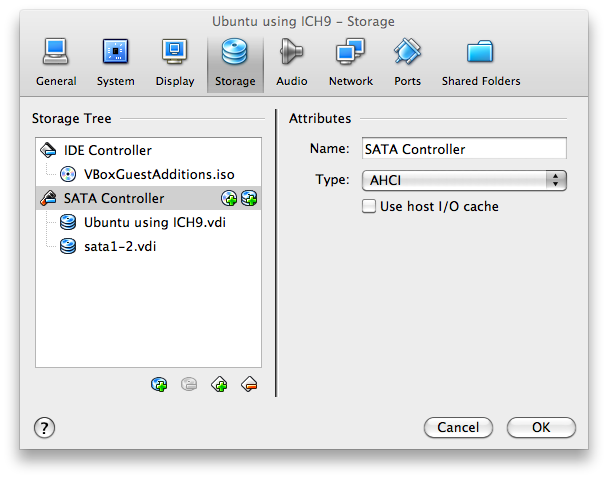
\includegraphics[width=10cm]{images/vm-settings-harddisk.png}
\end{center}

Depending on the guest operating system type that you selected when
    you created the VM, the typical layout of storage devices in a new VM is
    as follows:

\begin{itemize}


\item 

You will see an \textbf{IDE
          controller,} to which a virtual CD/DVD drive has been
          attached (to the \OQ{}secondary master\CQ{} port of the IDE
          controller).


\item 

You will also see a \textbf{SATA
          controller,} which is a more modern type of storage
          controller for higher hard disk data throughput, to which the
          virtual hard disks are attached. Initially you will normally have
          one such virtual disk, but as you can see in the above screenshot,
          you can have more than one, each represented by a disk image file
          (VDI files, in this case).

\end{itemize}


If you created your VM with an older version of VirtualBox, the
    default storage layout may differ. You might then only have an IDE
    controller to which both the CD/DVD drive and the hard disks have been
    attached. This might also apply if you selected an older operating system
    type when you created the VM. Since older operating systems do not support
    SATA without additional drivers, VirtualBox will make sure that no such
    devices are present initially. Please see chapter \ref{harddiskcontrollers}, \textit{\nameref{harddiskcontrollers}}, page \pageref{harddiskcontrollers} for additional information.

VirtualBox also provides a \textbf{floppy
    controller}, which is special: you cannot add devices other than
    floppy drives to it. Virtual floppy drives, like virtual CD/DVD drives,
    can be connected to either a host floppy drive (if you have one) or a disk
    image, which in this case must be in RAW format.

You can modify these media attachments freely. For example, if you
    wish to copy some files from another virtual disk that you created, you
    can connect that disk as a second hard disk, as in the above screenshot.
    You could also add a second virtual CD/DVD drive, or change where these
    items are attached. The following options are available:

\begin{itemize}


\item 

To \textbf{add another virtual hard disk, or a
          CD/DVD or floppy drive,} select the storage controller to
          which it should be added (IDE, SATA, SCSI, SAS, floppy controller)
          and then click on the \OQ{}add disk\CQ{} button below the tree. You can then
          either select \OQ{}Add CD/DVD device\CQ{} or \OQ{}Add Hard Disk\CQ{}. (If you
          clicked on a floppy controller, you can add a floppy drive instead.)
          Alternatively, right-click on the storage controller and select a
          menu item there.

On the right part of the window, you can then set the
          following:

\begin{enumerate}


\item 

You can then select to which \textbf{device slot} of the controller the
                virtual disk should be connected to. IDE controllers have four
                slots which have traditionally been called \OQ{}primary master\CQ{},
                \OQ{}primary slave\CQ{}, \OQ{}secondary master\CQ{} and \OQ{}secondary slave\CQ{}. By
                contrast, SATA and SCSI controllers offer you up to 30 slots
                to which virtual devices can be attached.


\item 

You can select which \textbf{image
                file} to use.

\begin{itemize}


\item 

For virtual hard disks, a button with a drop-down
                      list appears on the right, offering you to either select
                      a \textbf{virtual hard disk
                      file} using a standard file dialog or to
                      \textbf{create a new hard disk}
                      (image file), which will bring up the \OQ{}Create new disk\CQ{}
                      wizard, which was described in chapter \ref{gui-createvm}, \textit{\nameref{gui-createvm}}, page \pageref{gui-createvm}.

For details on the image file types that are
                      supported, please see chapter \ref{vdidetails}, \textit{\nameref{vdidetails}}, page \pageref{vdidetails}.


\item 

For virtual CD/DVD drives, the image files will
                      typically be in the standard ISO format instead. Most
                      commonly, you will select this option when installing an
                      operating system from an ISO file that you have obtained
                      from the Internet. For example, most Linux distributions
                      are available in this way.

For virtual CD/DVD drives, the following
                      additional options are available:



\begin{itemize}


\item 

If you select \textbf{\OQ{}Host
                            drive\CQ{}} from the list, then the physical
                            device of the host computer is connected to the VM,
                            so that the guest operating system can read from and
                            write to your physical device. This is, for
                            instance, useful if you want to install Windows from
                            a real installation CD. In this case, select your
                            host drive from the drop-down list presented.

If you want to write (burn) CDs or DVDs using
                            the host drive, you need to also enable the
                            \textbf{\OQ{}Passthrough\CQ{}}
                            option; see chapter \ref{storage-cds}, \textit{\nameref{storage-cds}}, page \pageref{storage-cds}.


\item 

If you select \textbf{\OQ{}Remove
                            disk from virtual drive\CQ{},} VirtualBox will
                            present an empty CD/DVD drive to the guest into
                            which no media has been inserted.

\end{itemize}


\end{itemize}


\end{enumerate}



\item 

To \textbf{remove an attachment,}
          select it and click on the \OQ{}remove\CQ{} icon at the bottom (or
          right-click on it and select the menu item).

\end{itemize}


Removable media (CD/DVDs and floppies) can be changed while the
    guest is running. Since the \OQ{}Settings\CQ{} dialog is not available at that
    time, you can also access these settings from the \OQ{}Devices\CQ{} menu of your
    virtual machine window.

\section{Audio settings}
\label{settings-audio}


The \OQ{}Audio\CQ{} section in a virtual machine's Settings window
    determines whether the VM will see a sound card connected, and whether the
    audio output should be heard on the host system.

If audio is enabled for a guest, you can choose between the
    emulation of an Intel AC'97 controller, an Intel HD Audio
    controller\footnote{Intel HD Audio support was added with VirtualBox 4.0 because
        Windows 7 (32-bit and 64-bit versions) as well as 64-bit Windows Vista
        do not support the Intel AC'97 controller.} or a SoundBlaster 16 card. In any case, you can select what
    audio driver VirtualBox will use on the host.

On a Linux host, depending on your host configuration, you can also
    select between the OSS, ALSA or the PulseAudio subsystem. On newer Linux
    distributions (Fedora 8 and above, Ubuntu 8.04 and above), the PulseAudio
    subsystem should be preferred.

\section{Network settings}
\label{settings-network}


The \OQ{}Network\CQ{} section in a virtual machine's Settings window allows
    you to configure how VirtualBox presents virtual network cards to your VM,
    and how they operate.

When you first create a virtual machine, VirtualBox by default
    enables one virtual network card and selects the \OQ{}Network Address
    Translation\CQ{} (NAT) mode for it. This way the guest can connect to the
    outside world using the host's networking and the outside world can
    connect to services on the guest which you choose to make visible outside
    of the virtual machine.

This default setup is good for probably 95\% of VirtualBox users.
    However, VirtualBox is extremely flexible in how it can virtualize
    networking. It supports many virtual network cards per virtual machine,
    the first four of which can be configured in detail in the Manager window.
    Additional network cards can be configured on the command line with
    VBoxManage. 

Because of the vast array of options available, we have dedicated an
    entire chapter of this manual to discussing networking configuration;
    please see chapter \ref{networkingdetails}, \textit{\nameref{networkingdetails}}, page \pageref{networkingdetails}.

\section{Serial ports}
\label{serialports}


VirtualBox fully supports virtual serial ports in a virtual machine
    in an easy-to-use manner.\footnote{Serial port support was added with VirtualBox 1.5.}

Ever since the original IBM PC, personal computers have been
    equipped with one or two serial ports (also called COM ports by DOS and
    Windows). Serial ports were commonly used with modems, and some
    computer mice used to be connected to serial ports before USB became 
    commonplace. 
    

While serial ports are no longer as ubiquitous as they used to be,
    there are still some important uses left for them. For example, serial
    ports can be used to set up a primitive network over a null-modem cable,
    in case Ethernet is not available. Also, serial ports are indispensable
    for system programmers needing to do kernel debugging, since kernel
    debugging software usually interacts with developers over a serial port.
    With virtual serial ports, system programmers can do kernel debugging on a
    virtual machine instead of needing a real computer to connect to.

If a virtual serial port is enabled, the guest operating system sees
    a standard 16550A compatible UART device. Both receiving and transmitting
    data is supported. How this virtual serial port is then connected to the 
    host is configurable, and the details depend on your host operating system.
    

You can use either the graphical user interface or the command-line
    \texttt{VBoxManage} tool to set up virtual serial
    ports. For the latter, please refer to chapter \ref{vboxmanage-modifyvm}, \textit{\nameref{vboxmanage-modifyvm}}, page \pageref{vboxmanage-modifyvm}; in that section, look for the
    \texttt{-{}-uart} and
    \texttt{-{}-uartmode} options.

In either case, you can configure up to two virtual serial ports per 
    virtual machine. For each such device, you will need to
    determine

\begin{enumerate}


\item 

what kind of serial port the virtual machine should see by
          selecting an I/O base address and interrupt (IRQ). For these, we
          recommend to use the traditional values\footnote{See, for example, \url{http://en.wikipedia.org/wiki/COM\_(hardware\_interface)}.}, which are:



\begin{enumerate}


\item 

COM1: I/O base 0x3F8, IRQ 4


\item 

COM2: I/O base 0x2F8, IRQ 3


\item 

COM3: I/O base 0x3E8, IRQ 4


\item 

COM4: I/O base 0x2E8, IRQ 3

\end{enumerate}



\item 

Then, you will need to determine what this virtual port should
          be connected to. For each virtual serial port, you have the
          following options:



\begin{itemize}


\item 

You can elect to have the virtual serial port
                \OQ{}disconnected\CQ{}, which means that the guest will see the
                device, but it will behave as if no cable had been connected
                to it.


\item 

You can connect the virtual serial port to a physical
                serial port on your host. (On a Windows host, this will be a
                name like \texttt{COM1}; on Linux or
                Solaris hosts, it will be a device node like
                \texttt{/dev/ttyS0}). VirtualBox will
                then simply redirect all data received from and sent to the
                virtual serial port to the physical device.


\item 

You can tell VirtualBox to connect the virtual serial
                port to a software pipe on the host. This depends on your host
                operating system:

\begin{itemize}


\item 

On a Windows host, data will be sent and received
                      through a named pipe. The pipe name must be in the format
                      \texttt{\textbackslash{}\textbackslash{}.\textbackslash{}pipe\textbackslash{}<name>} 
                      where \texttt{<name>} should
                      identify the virtual machine but may be freely 
                      chosen.

For forwarding serial traffic, you can use a helper
                      program called VMware Serial Line Gateway, available for
                      download at
                                  \url{http://www.l4ka.org/91.php}. This tool provides a fixed server mode named
                      pipe at
                      \texttt{\textbackslash{}\textbackslash{}.\textbackslash{}pipe\textbackslash{}vmwaredebug}
                      and connects incoming TCP connections on port 567 with
                      the named pipe.


\item 

On a Mac, Linux or Solaris host, a local
                      domain socket is used instead. The socket filename must be
                      chosen such that the user running VirtualBox has 
                      sufficient privileges to create and write to it. The 
                      \texttt{/tmp} directory is often a 
                      good candidate.

On Linux there are various tools which can connect 
                      to a local domain socket or create one in server mode. The 
                      most flexible tool is
                      \texttt{socat} and is available
                      as part of many distributions.

\end{itemize}


In this case, you can configure whether VirtualBox
                should create the named pipe (or, on non-Windows hosts, the
                local domain socket) itself or whether VirtualBox should
                assume that the pipe (or socket) exists already. With the
                \texttt{VBoxManage} command-line
                options, this is referred to as \OQ{}server\CQ{} or \OQ{}client\CQ{} mode,
                respectively.

For a direct connection between two virtual machines
                (corresponding to a null-modem cable), simply configure one VM 
                to create a pipe/socket and another to attach to it.
                


\item 

You can send the virtual serial port output to a file. 
                This option is very useful for capturing diagnostic output from 
                a guest. Any file may be used for this purpose, as long as the 
                user running VirtualBox has sufficient privileges to create and 
                write to the file.
                

\end{itemize}


\end{enumerate}
Up to two serial ports can be configured per virtual 
      machine, but you can pick any port numbers out of the above. However,
      serial ports cannot reliably share interrupts; if both ports are to be 
      used at the same time, they must use different interrupt levels, for 
      example COM1 and COM2, but not COM1 and COM3.
    

\section{USB support}


\subsection{USB settings}
\label{settings-usb}


The \OQ{}USB\CQ{} section in a virtual machine's Settings window allows
      you to configure VirtualBox's sophisticated USB support.

VirtualBox can allow virtual machines to access the USB devices on
      your host directly. To achieve this, VirtualBox presents the guest
      operating system with a virtual USB controller. As soon as the guest
      system starts using a USB device, it will appear as unavailable on the
      host.

\vspace{.2cm}

\begin{center}\fbox{\begin{minipage}[c]{0.9\textwidth}\color{colNote}\textbf{Note:} 

\begin{enumerate}


\item 

Be careful with USB devices that are currently in use on
              the host! For example, if you allow your guest to connect to
              your USB hard disk that is currently mounted on the host, when
              the guest is activated, it will be disconnected from the host
              without a proper shutdown. This may cause data loss.


\item 

Solaris hosts have a few known limitations regarding USB
              support; please see chapter \ref{KnownIssues}, \textit{\nameref{KnownIssues}}, page \pageref{KnownIssues}.

\end{enumerate}
\end{minipage}}\end{center}

\vspace{.2cm}



In addition to allowing a guest access to your local USB devices,
      VirtualBox even allows your guests to connect to remote USB devices by
      use of the VirtualBox Remote Desktop Extension (VRDE). For details about
      this, see chapter \ref{usb-over-rdp}, \textit{\nameref{usb-over-rdp}}, page \pageref{usb-over-rdp}.

In the Settings dialog, you can first configure whether USB is
      available in the guest at all, and in addition also optionally enable
      the USB 2.0 (EHCI) controller for the guest. If so, you can determine in
      detail which devices are available. For this, you must create so-called
      \OQ{}filters\CQ{} by specifying certain properties of the USB device.

\vspace{.2cm}

\begin{center}\fbox{\begin{minipage}[c]{0.9\textwidth}\color{colNote}\textbf{Note:} The EHCI controller is shipped as a VirtualBox extension
          package, which must be installed separately. See chapter \ref{intro-installing}, \textit{\nameref{intro-installing}}, page \pageref{intro-installing} for more information.\end{minipage}}\end{center}

\vspace{.2cm}



When USB support is enabled for a VM, you can determine in detail
      which devices will be automatically attached to the guest. For this, you
      can create so-called \OQ{}filters\CQ{} by specifying certain properties of
      the USB device. USB devices with a matching filter will be automatically
      passed to the guest once they are attached to the host. USB devices
      without a matching filter can be passed manually to the guest, for
      example by using the Devices / USB devices menu.

Clicking on the \OQ{}+\OQ{} button to the right of the \OQ{}USB Device
      Filters\CQ{} window creates a \textbf{new filter.}
      You can give the filter a name (for referencing it later) and specify
      the filter criteria. The more criteria you specify, the more precisely
      devices will be selected. For instance, if you specify only a vendor ID
      of 046d, all devices produced by Logitech will be available to the
      guest. If you fill in all fields, on the other hand, the filter will
      only apply to a particular device model from a particular vendor, and
      not even to other devices of the same type with a different revision and
      serial number.

In detail, the following criteria are available:

\begin{enumerate}


\item 

\textbf{Vendor and product ID.} With
          USB, each vendor of USB products carries an identification number
          that is unique world-wide, the \OQ{}vendor ID\CQ{}. Similarly, each line of
          products is assigned a \OQ{}product ID\CQ{} number. Both numbers are
          commonly written in hexadecimal (that is, they are composed of the
          numbers 0-9 and the letters A-F), and a colon separates the vendor
          from the product ID. For example,
          \texttt{046d:c016} stands for Logitech as a
          vendor, and the \OQ{}M-UV69a Optical Wheel Mouse\CQ{} product.

Alternatively, you can also specify \textbf{\OQ{}Manufacturer\CQ{}} and \textbf{\OQ{}Product\CQ{}} by name.

To list all the USB devices that are connected to your host
          machine with their respective vendor and product IDs, you can use
          the following command (see chapter \ref{vboxmanage}, \textit{\nameref{vboxmanage}}, page \pageref{vboxmanage}): 

\begin{Verbatim}[fontsize=\footnotesize]
VBoxManage list usbhost
\end{Verbatim}


On Windows, you can also see all USB devices that are attached
          to your system in the Device Manager. On Linux, you can use the
          \texttt{lsusb} command.


\item 

\textbf{Serial number.} While vendor
          and product ID are already quite specific to identify USB devices,
          if you have two identical devices of the same brand and product
          line, you will also need their serial numbers to filter them out
          correctly.


\item 

\textbf{Remote.} This setting
          specifies whether the device will be local only, or remote only
          (over VRDP), or either.

\end{enumerate}


On a Windows host, you will need to unplug and reconnect a USB
      device to use it after creating a filter for it.

As an example, you could create a new USB filter and specify a
      vendor ID of 046d (Logitech, Inc), a manufacturer index of 1, and \OQ{}not
      remote\CQ{}. Then any USB devices on the host system produced by Logitech,
      Inc with a manufacturer index of 1 will be visible to the guest
      system.

Several filters can select a single device -- for example, a
      filter which selects all Logitech devices, and one which selects a
      particular webcam.

You can \textbf{deactivate} filters
      without deleting them by clicking in the checkbox next to the filter
      name.

\subsection{Implementation notes for Windows and Linux hosts}


On Windows hosts, a kernel mode device driver provides USB proxy
      support. It implements both a USB monitor, which allows VirtualBox to
      capture devices when they are plugged in, and a USB device driver to
      claim USB devices for a particular virtual machine. As opposed to
      VirtualBox versions before 1.4.0, system reboots are no longer necessary
      after installing the driver. Also, you no longer need to replug devices
      for VirtualBox to claim them.

On newer Linux hosts, VirtualBox accesses USB devices through
      special files in the file system. When VirtualBox is installed, these
      are made available to all users in the
      \texttt{vboxusers} system group. In order to be
      able to access USB from guest systems, make sure that you are a member
      of this group.

On older Linux hosts, USB devices are accessed using the
      \texttt{usbfs} file system. Therefore, the user
      executing VirtualBox needs read and write permission to the USB file
      system. Most distributions provide a group (e.g.
      \texttt{usbusers}) which the VirtualBox user
      needs to be added to. Also, VirtualBox can only proxy to virtual
      machines USB devices which are not claimed by a Linux host USB driver.
      The \texttt{Driver=} entry in
      \texttt{/proc/bus/usb/devices} will show you
      which devices are currently claimed. Please refer to chapter \ref{ts_usb-linux}, \textit{\nameref{ts_usb-linux}}, page \pageref{ts_usb-linux} also for details about
      \texttt{usbfs}.

\section{Shared folders}


Shared folders allow you to easily exchange data between a virtual
    machine and your host. This feature requires that the VirtualBox Guest
    Additions be installed in a virtual machine and is described in detail in
    chapter \ref{sharedfolders}, \textit{\nameref{sharedfolders}}, page \pageref{sharedfolders}.

\section{Alternative firmware (EFI)}
\label{efi}


Starting with release 3.1, VirtualBox includes experimental support
    for the Extensible Firmware Interface (EFI), which is a new industry
    standard intended to eventually replace the legacy BIOS as the primary
    interface for bootstrapping computers and certain system services
    later.

By default, VirtualBox uses the BIOS firmware for virtual machines.
    To use EFI for a given virtual machine, you can enable EFI in the
    machine's \OQ{}Settings\CQ{} dialog (see chapter \ref{settings-motherboard}, \textit{\nameref{settings-motherboard}}, page \pageref{settings-motherboard}).
    Alternatively, use the \texttt{VBoxManage} command
    line interface like this: 

\begin{Verbatim}[fontsize=\footnotesize]
VBoxManage modifyvm "VM name" --firmware efi
\end{Verbatim}

    To switch back to using the BIOS, use: 

\begin{Verbatim}[fontsize=\footnotesize]
VBoxManage modifyvm "VM name" --firmware bios
\end{Verbatim}
One
    notable user of EFI is Apple's Mac OS X, but recent Linuxes (such as Fedora
    11) and Windows (starting with Vista) offer special versions that can be
    booted using EFI as well.

Another possible use of EFI in VirtualBox is development and testing
    of EFI applications, without booting any OS.

Note that the VirtualBox EFI support is experimental and will be
    enhanced as EFI matures and becomes more widespread. While Mac OS X and
    Linux guests are known to work fine, Windows guests are currently unable
    to boot with the VirtualBox EFI implementation.

\subsection{Video modes in EFI}
\label{efividmode}


EFI provides two distinct video interfaces: GOP (Graphics Output
      Protocol) and UGA (Universal Graphics Adapter). Mac OS X uses GOP, while
      Linux tends to use UGA. VirtualBox provides a configuration option to
      control the framebuffer size for both interfaces.

To control GOP, use the following
      \texttt{VBoxManage} command: 

\begin{Verbatim}[fontsize=\footnotesize]
VBoxManage setextradata "VM name" VBoxInternal2/EfiGopMode N
\end{Verbatim}

      Where N can be one of 0,1,2,3,4,5 referring to the 640x480, 800x600,
      1024x768, 1280x1024, 1440x900, 1920x1200 screen resolution respectively.

To change the UGA resolution: 

\begin{Verbatim}[fontsize=\footnotesize]
VBoxManage setextradata "VM name" VBoxInternal2/UgaHorizontalResolution 1440
VBoxManage setextradata "VM name" VBoxInternal2/UgaVerticalResolution    900
\end{Verbatim}


The video mode for both GOP and UGA can only be changed when the
      VM is powered off and remains persistent until changed.

\subsection{Specifying boot arguments}
\label{efibootargs}


It is currently not possible to manipulate EFI variables from within a running guest
      (e.g., setting the \OQ{}boot-args\CQ{} variable by running the \texttt{nvram} tool in a Mac OS X guest will not work).
      As an alternative way, \OQ{}VBoxInternal2/EfiBootArgs\CQ{} extradata can be passed to a VM in order to set
      the \OQ{}boot-args\CQ{} variable. To change the \OQ{}boot-args\CQ{} EFI variable:
      

\begin{Verbatim}[fontsize=\footnotesize]
VBoxManage setextradata "VM name" VBoxInternal2/EfiBootArgs <value>
\end{Verbatim}

      

\chapter{Guest Additions}
\label{guestadditions}


The previous chapter covered getting started with VirtualBox and
  installing operating systems in a virtual machine. For any serious and
  interactive use, the VirtualBox Guest Additions will make your life much
  easier by providing closer integration between host and guest and improving
  the interactive performance of guest systems. This chapter describes the
  Guest Additions in detail.

\section{Introduction}


As mentioned in chapter \ref{virtintro}, \textit{\nameref{virtintro}}, page \pageref{virtintro}, the Guest Additions
    are designed to be installed \textit{inside} a virtual machine
    after the guest operating system has been installed. They consist of
    device drivers and system applications that optimize the guest operating
    system for better performance and usability. Please see chapter \ref{guestossupport}, \textit{\nameref{guestossupport}}, page \pageref{guestossupport} for details on what guest operating systems
    are fully supported with Guest Additions by VirtualBox.

The VirtualBox Guest Additions for all supported guest operating
    systems are provided as a single CD-ROM image file which is called
    \texttt{VBoxGuestAdditions.iso}. This image file
    is located in the installation directory of VirtualBox. To install the
    Guest Additions for a particular VM, you mount this ISO file in your VM as
    a virtual CD-ROM and install from there.

The Guest Additions offer the following features:

\begin{description}


\item[Mouse pointer integration]

To overcome the limitations for mouse support that were
            described in chapter \ref{keyb_mouse_normal}, \textit{\nameref{keyb_mouse_normal}}, page \pageref{keyb_mouse_normal}, this provides
            you with seamless mouse support. You will only have one mouse
            pointer and pressing the Host key is no longer required to \OQ{}free\CQ{}
            the mouse from being captured by the guest OS. To make this work,
            a special mouse driver is installed in the guest that communicates
            with the \OQ{}real\CQ{} mouse driver on your host and moves the guest
            mouse pointer accordingly.

\item[Shared folders]

These provide an easy way to exchange files between the host
            and the guest. Much like ordinary Windows network shares, you can
            tell VirtualBox to treat a certain host directory as a shared
            folder, and VirtualBox will make it available to the guest
            operating system as a network share, irrespective of whether guest
            actually has a network. For details, please refer to chapter \ref{sharedfolders}, \textit{\nameref{sharedfolders}}, page \pageref{sharedfolders}.

\item[Better video support]

While the virtual graphics card which VirtualBox emulates
            for any guest operating system provides all the basic features,
            the custom video drivers that are installed with the Guest
            Additions provide you with extra high and non-standard video modes
            as well as accelerated video performance.

In addition, with Windows, Linux and Solaris guests, you can
            resize the virtual machine's window if the Guest Additions are
            installed. The video resolution in the guest will be automatically
            adjusted (as if you had manually entered an arbitrary resolution
            in the guest's display settings). Please see chapter \ref{intro-resize-window}, \textit{\nameref{intro-resize-window}}, page \pageref{intro-resize-window} also.

Finally, if the Guest Additions are installed, 3D graphics
            and 2D video for guest applications can be accelerated; see chapter \ref{guestadd-video}, \textit{\nameref{guestadd-video}}, page \pageref{guestadd-video}.

\item[Seamless windows]

With this feature, the individual windows that are displayed
            on the desktop of the virtual machine can be mapped on the host's
            desktop, as if the underlying application was actually running on
            the host. See chapter \ref{seamlesswindows}, \textit{\nameref{seamlesswindows}}, page \pageref{seamlesswindows} for
            details.

\item[Generic host/guest communication channels]

The Guest Additions enable you to control and monitor guest
            execution in ways other than those mentioned above. The so-called
            \OQ{}guest properties\CQ{} provide a generic string-based mechanism to
            exchange data bits between a guest and a host, some of which have
            special meanings for controlling and monitoring the guest; see
            chapter \ref{guestadd-guestprops}, \textit{\nameref{guestadd-guestprops}}, page \pageref{guestadd-guestprops} for details.

Additionally, applications can be started in a guest from
            the host; see chapter \ref{guestadd-guestcontrol}, \textit{\nameref{guestadd-guestcontrol}}, page \pageref{guestadd-guestcontrol}.

\item[Time synchronization]

With the Guest Additions installed, VirtualBox can ensure
            that the guest's system time is better synchronized with that of
            the host.

For various reasons, the time in the guest might run at a
            slightly different rate than the time on the host. The host could
            be receiving updates via NTP and its own time might not run
            linearly. A VM could also be paused, which stops the flow of time
            in the guest for a shorter or longer period of time. When the wall
            clock time between the guest and host only differs slightly, the
            time synchronization service attempts to gradually and smoothly
            adjust the guest time in small increments to either \OQ{}catch up\CQ{} or
            \OQ{}lose\CQ{} time. When the difference is too great (e.g., a VM paused
            for hours or restored from saved state), the guest time is changed
            immediately, without a gradual adjustment.

The Guest Additions will re-synchronize the time regularly.
            See chapter \ref{changetimesync}, \textit{\nameref{changetimesync}}, page \pageref{changetimesync} for how to configure the
            parameters of the time synchronization mechanism.

\item[Shared clipboard]

With the Guest Additions installed, the clipboard of the
            guest operating system can optionally be shared with your host
            operating system; see chapter \ref{generalsettings}, \textit{\nameref{generalsettings}}, page \pageref{generalsettings}.

\item[Automated logons (credentials passing)]

For details, please see chapter \ref{autologon}, \textit{\nameref{autologon}}, page \pageref{autologon}.
\end{description}


Each version of VirtualBox, even minor releases, ship with their own
    version of the Guest Additions. While the interfaces through which the
    VirtualBox core communicates with the Guest Additions are kept stable so
    that Guest Additions already installed in a VM should continue to work
    when VirtualBox is upgraded on the host, for best results, it is
    recommended to keep the Guest Additions at the same version.

Starting with VirtualBox 3.1, the Windows and Linux Guest Additions
    therefore check automatically whether they have to be updated. If the host
    is running a newer VirtualBox version than the Guest Additions, a
    notification with further instructions is displayed in the guest.

To disable this update check for the Guest Additions of a given
    virtual machine, set the value of its
    \texttt{/VirtualBox/GuestAdd/CheckHostVersion}
    guest property to \texttt{0}; see chapter \ref{guestadd-guestprops}, \textit{\nameref{guestadd-guestprops}}, page \pageref{guestadd-guestprops} for details.

\section{Installing and Maintaining Guest Additions}


Guest Additions are available for virtual machines running Windows,
    Linux, Solaris or OS/2. The following sections describe the specifics of
    each variant in detail.

\subsection{Guest Additions for Windows}
\label{additions-windows}


The VirtualBox Windows Guest Additions are designed to be
      installed in a virtual machine running a Windows operating system. The
      following versions of Windows guests are supported:

\begin{itemize}


\item 

Microsoft Windows NT 4.0 (any service pack)


\item 

Microsoft Windows 2000 (any service pack)


\item 

Microsoft Windows XP (any service pack)


\item 

Microsoft Windows Server 2003 (any service pack)


\item 

Microsoft Windows Server 2008


\item 

Microsoft Windows Vista (all editions)


\item 

Microsoft Windows 7 (all editions)


\item 

Microsoft Windows 8 (all editions)


\item 

Microsoft Windows Server 2012

\end{itemize}


\subsubsection{Installation}
\label{mountingadditionsiso}


In the \OQ{}Devices\CQ{} menu in the virtual machine's menu bar,
        VirtualBox has a handy menu item named \OQ{}Insert Guest Additions CD image\CQ{},
        which mounts the Guest Additions ISO file inside your virtual machine.
        A Windows guest should then automatically start the Guest Additions
        installer, which installs the Guest Additions into your Windows
        guest. Other guest operating systems (or if automatic start of
        software on CD is disabled) need manual start of the installer.

\vspace{.2cm}

\begin{center}\fbox{\begin{minipage}[c]{0.9\textwidth}\color{colNote}\textbf{Note:} For the basic Direct3D acceleration to work in a Windows Guest, you
          have to install the Guest Additions in \OQ{}Safe Mode\CQ{}.
          This does \textbf{not} apply to the experimental
          WDDM Direct3D video driver available
          for Vista and Windows 7 guests, see chapter \ref{KnownIssues}, \textit{\nameref{KnownIssues}}, page \pageref{KnownIssues} for
          details.\footnote{The experimental WDDM driver was added with
          VirtualBox 4.1.}\end{minipage}}\end{center}

\vspace{.2cm}



If you prefer to mount the additions manually, you can perform
        the following steps:

\begin{enumerate}


\item 

Start the virtual machine in which you have installed
            Windows.


\item 

Select \OQ{}Mount CD/DVD-ROM\CQ{} from the \OQ{}Devices\CQ{} menu in the
            virtual machine's menu bar and then \OQ{}CD/DVD-ROM image\CQ{}. This
            brings up the Virtual Media Manager described in chapter \ref{vdis}, \textit{\nameref{vdis}}, page \pageref{vdis}.


\item 

In the Virtual Media Manager, press the \OQ{}Add\CQ{} button and
            browse your host file system for the
            \texttt{VBoxGuestAdditions.iso}
            file:

\begin{itemize}


\item 

On a Windows host, you can find this file in the
                  VirtualBox installation directory (usually under
                  \texttt{C:\textbackslash{}Program
                  files\textbackslash{}Oracle\textbackslash{}VirtualBox} ).


\item 

On Mac OS X hosts, you can find this file in the
                  application bundle of VirtualBox. (Right click on the
                  VirtualBox icon in Finder and choose \textit{Show Package
                  Contents}. There it is located in the
                  \texttt{Contents/MacOS}
                  folder.)


\item 

On a Linux host, you can find this file in the
                  \texttt{additions} folder under
                  where you installed VirtualBox (normally
                  \texttt{/opt/VirtualBox/}).


\item 

On Solaris hosts, you can find this file in the
                  \texttt{additions} folder under
                  where you installed VirtualBox (normally
                  \texttt{/opt/VirtualBox}).

\end{itemize}



\item 

Back in the Virtual Media Manager, select that ISO file and
            press the \OQ{}Select\CQ{} button. This will mount the ISO file and
            present it to your Windows guest as a CD-ROM.

\end{enumerate}


Unless you have the Autostart feature disabled in your Windows
        guest, Windows will now autostart the VirtualBox Guest Additions
        installation program from the Additions ISO. If the Autostart feature
        has been turned off, choose
        \texttt{VBoxWindowsAdditions.exe} from the
        CD/DVD drive inside the guest to start the installer.

The installer will add several device drivers to the Windows
        driver database and then invoke the hardware detection wizard.

Depending on your configuration, it might display warnings that
        the drivers are not digitally signed. You must confirm these in order
        to continue the installation and properly install the
        Additions.

After installation, reboot your guest operating system to
        activate the Additions.

\subsubsection{Updating the Windows Guest Additions}


Windows Guest Additions can be updated by running the
        installation program again, as previously described. This will then
        replace the previous Additions drivers with updated versions.

Alternatively, you may also open the Windows Device Manager and
        select \OQ{}Update driver...\OQ{} for two devices:

\begin{enumerate}


\item 

the VirtualBox Graphics Adapter and


\item 

the VirtualBox System Device.

\end{enumerate}


For each, choose to provide your own driver and use \OQ{}Have Disk\CQ{}
        to point the wizard to the CD-ROM drive with the Guest
        Additions.

\subsubsection{Unattended Installation}


As a prerequiste for performing an unattended installation of the
        VirtualBox Guest Additions on a Windows guest, there need to be
        Oracle CA (Certificate Authority)
        certificates installed in order to prevent user intervention popus which
        will undermine a silent installation.

\vspace{.2cm}

\begin{center}\fbox{\begin{minipage}[c]{0.9\textwidth}\color{colNote}\textbf{Note:} On some Windows versions like Windows 2000 and Windows XP the user intervention
        popups mentioned above always will be displayed, even after importing the Oracle certificates.\end{minipage}}\end{center}

\vspace{.2cm}



Since VirtualBox 4.2 installing those CA certificates on a Windows
        guest can be done in an automated fashion using the
        \texttt{VBoxCertUtil.exe} utility found on the Guest
        Additions installation CD in the \texttt{cert}
        folder:

\begin{itemize}


\item 

Log in as Administrator on the guest.


\item 

Mount the VirtualBox Guest Additions .ISO.


\item 

Open a command line window on the guest and change to
            the \texttt{cert} folder on the VirtualBox
            Guest Additions CD.


\item 

Do

\begin{Verbatim}[fontsize=\footnotesize]
VBoxCertUtil add-trusted-publisher oracle-vbox.cer --root oracle-vbox.cer
\end{Verbatim}


This will install the certificates to the certificate store. When installing the same certificate
            more than once, an appropriate error will be displayed.

\end{itemize}


Prior to VirtualBox 4.2 the Oracle CA certificates need to be imported in more manual style
        using the \texttt{certutil.exe} utility, which is shipped since Windows
        Vista. For Windows versions before Vista you need to download and install \texttt{certutil.exe}
        manually. Since the certificates are not accompanied on the VirtualBox Guest Additions CD-ROM
        prior to 4.2, these need to get extracted from a signed VirtualBox executable first.

In the following example the needed certificates will be extracted from the VirtualBox
        Windows Guest Additions installer on the CD-ROM:

\paragraph{VeriSign Code Signing CA}


\begin{itemize}


\item 

In the Windows Explorer, right click on VBoxWindowsAdditions-<Architecture>.exe,
              click on \OQ{}Properties\CQ{}


\item 

Go to tab \OQ{}Digital Signatures\CQ{}, choose \OQ{}Oracle Corporation\CQ{} and click on \OQ{}Details\CQ{}


\item 

In tab \OQ{}General\CQ{} click on \OQ{}View Certificate\CQ{}


\item 

In tab \OQ{}Certification Path\CQ{} select \OQ{}VeriSign Class 3 Public Primary CA\CQ{}


\item 

Click on \OQ{}View Certificate\CQ{}


\item 

In tab \OQ{}Details\CQ{} click on \OQ{}Copy to File ...\OQ{}


\item 

In the upcoming wizard choose \OQ{}DER encoded binary X.509 (.CER)\OQ{}
              and save the certificate file to a local path, finish the wizard


\item 

Close certificate dialog for \OQ{}Verisign Class 3 Code Signing
              2010 CA\CQ{}

\end{itemize}


\paragraph{Oracle Corporation}


\begin{itemize}


\item 

In the Windows Explorer, right click on VBoxWindowsAdditions-<Architecture>.exe,
              click on \OQ{}Properties\CQ{}


\item 

Go to tab \OQ{}Digital Signatures\CQ{}, choose \OQ{}Oracle Corporation\CQ{} and click on \OQ{}Details\CQ{}


\item 

In tab \OQ{}General\CQ{} click on \OQ{}View Certificate\CQ{}


\item 

In tab \OQ{}Details\CQ{} click on \OQ{}Copy to File ...\OQ{}


\item 

In the upcoming wizard choose \OQ{}DER encoded binary X.509 (.CER)\OQ{}
              and save the certificate file to a local path, finish the wizard


\item 

Close certificate dialog for \OQ{}Oracle Corporation\CQ{}

\end{itemize}


After exporting the two certificates above they can be imported into the
        certificate store using the \texttt{certutil.exe}
        utility:

\texttt{certutil -addstore -f Root "<Path to exported
        certificate file>"}

In order to allow for completely unattended guest installations,
        you can specify a command line parameter to the install
        launcher:

\begin{Verbatim}[fontsize=\footnotesize]
VBoxWindowsAdditions.exe /S
\end{Verbatim}


This automatically installs the right files and drivers for the
        corresponding platform (32- or 64-bit).

\vspace{.2cm}

\begin{center}\fbox{\begin{minipage}[c]{0.9\textwidth}\color{colNote}\textbf{Note:} By default on an unattended installation on a Windows 7 or 8
        guest, there will be the XPDM graphics driver installed. This graphics
        driver does not support Windows Aero / Direct3D on the guest - instead the
        experimental WDDM graphics driver needs to be installed. To select this
        driver by default, add the command line parameter
        \texttt{/with\_wddm} when invoking the Windows
        Guest Additions installer.\end{minipage}}\end{center}

\vspace{.2cm}



\vspace{.2cm}

\begin{center}\fbox{\begin{minipage}[c]{0.9\textwidth}\color{colNote}\textbf{Note:} For Windows Aero to run correctly on a guest, the guest's
        VRAM size needs to be configured to at least 128 MB.\end{minipage}}\end{center}

\vspace{.2cm}



For more options regarding unattended guest installations,
        consult the command line help by using the command:

\begin{Verbatim}[fontsize=\footnotesize]
VBoxWindowsAdditions.exe /?
\end{Verbatim}


\subsubsection{Manual file extraction}
\label{windows-guest-file-extraction}


If you would like to install the files and drivers manually, you
        can extract the files from the Windows Guest Additions setup by
        typing:

\begin{Verbatim}[fontsize=\footnotesize]
VBoxWindowsAdditions.exe /extract
\end{Verbatim}


To explicitly extract the Windows Guest Additions for another
        platform than the current running one (e.g. 64-bit files on a 32-bit
        system), you have to execute the appropriate platform installer
        (\texttt{VBoxWindowsAdditions-x86.exe} or
        \texttt{VBoxWindowsAdditions-amd64.exe}) with
        the \texttt{/extract} parameter.

\subsection{Guest Additions for Linux}


Like the Windows Guest Additions, the VirtualBox Guest Additions
      for Linux are a set of device drivers and system applications which may
      be installed in the guest operating system.

The following Linux distributions are officially supported:

\begin{itemize}


\item 

Oracle Linux as of version 5 including UEK kernels;


\item 

Fedora as of Fedora Core 4;


\item 

Redhat Enterprise Linux as of version 3;


\item 

SUSE and openSUSE Linux as of version 9;


\item 

Ubuntu as of version 5.10.

\end{itemize}


Many other distributions are known to work with the Guest
      Additions.

The version of the Linux kernel supplied by default in SUSE and
      openSUSE 10.2, Ubuntu 6.10 (all versions) and Ubuntu 6.06 (server
      edition) contains a bug which can cause it to crash during startup when
      it is run in a virtual machine. The Guest Additions work in those
      distributions.

Note that some Linux distributions already come with all or part of
      the VirtualBox Guest Additions. You may choose to keep the distribution's
      version of the Guest Additions but these are often not up to date and
      limited in functionality, so we recommend replacing them with the
      Guest Additions that come with VirtualBox. The VirtualBox Linux Guest
      Additions installer tries to detect existing installation and replace
      them but depending on how the distribution integrates the Guest
      Additions, this may require some manual interaction. It is highly
      recommended to take a snapshot of the virtual machine before replacing
      pre-installed Guest Additions.

\subsubsection{Installing the Linux Guest Additions}


The VirtualBox Guest Additions for Linux are provided on the
        same virtual CD-ROM file as the Guest Additions for Windows described
        above. They also come with an installation program guiding you through
        the setup process, although, due to the significant differences between
        Linux distributions, installation may be slightly more complex.

Installation generally involves the following steps:

\begin{enumerate}


\item 

Before installing the Guest Additions, you will have to
            prepare your guest system for building external kernel modules.
            This works similarly as described in chapter \ref{externalkernelmodules}, \textit{\nameref{externalkernelmodules}}, page \pageref{externalkernelmodules}, except that this step must now
            be performed in your Linux \textit{guest} instead of
            on a Linux host system, as described there.

Again, as with Linux hosts, we recommend using DKMS if it is
            available for the guest system. If it is not installed, use this
            command for Ubuntu/Debian systems:
            

\begin{Verbatim}[fontsize=\footnotesize]
sudo apt-get install dkms
\end{Verbatim}

            or for Fedora systems: 

\begin{Verbatim}[fontsize=\footnotesize]
yum install dkms
\end{Verbatim}


Be sure to install DKMS \textit{before}
            installing the Linux Guest Additions. If DKMS is not available
            or not installed, the guest kernel modules will need to be
            recreated manually whenever the guest kernel is updated using
            the command 

\begin{Verbatim}[fontsize=\footnotesize]
/etc/init.d/vboxadd setup
\end{Verbatim}
 as root.
            


\item 

Insert the
            \texttt{VBoxGuestAdditions.iso} CD file
            into your Linux guest's virtual CD-ROM drive, exactly the same way
            as described for a Windows guest in chapter \ref{mountingadditionsiso}, \textit{\nameref{mountingadditionsiso}}, page \pageref{mountingadditionsiso}.


\item 

Change to the directory where your CD-ROM drive is mounted
            and execute as root:

\begin{Verbatim}[fontsize=\footnotesize]
sh ./VBoxLinuxAdditions.run
\end{Verbatim}


\end{enumerate}


For your convenience, we provide the following step-by-step
        instructions for freshly installed copies of recent versions of the most
        popular Linux distributions. After these preparational steps, you can
        execute the VirtualBox Guest Additions installer as described
        above.

\paragraph{Ubuntu}




\begin{enumerate}


\item 

In order to fully update your guest system, open a
                terminal and run 

\begin{Verbatim}[fontsize=\footnotesize]
apt-get update
\end{Verbatim}
 as root
                followed by 

\begin{Verbatim}[fontsize=\footnotesize]
apt-get upgrade
\end{Verbatim}



\item 

Install DKMS using 

\begin{Verbatim}[fontsize=\footnotesize]
apt-get install dkms
\end{Verbatim}



\item 

Reboot your guest system in order to activate the
                updates and then proceed as described above.

\end{enumerate}


\paragraph{Fedora}




\begin{enumerate}


\item 

In order to fully update your guest system, open a
                terminal and run 

\begin{Verbatim}[fontsize=\footnotesize]
yum update
\end{Verbatim}
 as root.
              


\item 

Install DKMS and the GNU C compiler using 

\begin{Verbatim}[fontsize=\footnotesize]
yum install dkms
\end{Verbatim}

                followed by 

\begin{Verbatim}[fontsize=\footnotesize]
yum install gcc
\end{Verbatim}



\item 

Reboot your guest system in order to activate the
                updates and then proceed as described above.

\end{enumerate}


\paragraph{openSUSE}




\begin{enumerate}


\item 

In order to fully update your guest system, open a
                terminal and run 

\begin{Verbatim}[fontsize=\footnotesize]
zypper update
\end{Verbatim}
 as root.
              


\item 

Install the make tool and the GNU C compiler using
                

\begin{Verbatim}[fontsize=\footnotesize]
zypper install make gcc
\end{Verbatim}



\item 

Reboot your guest system in order to activate the
                updates.


\item 

Find out which kernel you are running using 

\begin{Verbatim}[fontsize=\footnotesize]
uname -a
\end{Verbatim}

                An example would be
                \texttt{2.6.31.12-0.2-default} which
                refers to the \OQ{}default\CQ{} kernel. Then install the correct
                kernel development package. In the above example this would be
                

\begin{Verbatim}[fontsize=\footnotesize]
zypper install kernel-default-devel
\end{Verbatim}



\item 

Make sure that your running kernel
                (\texttt{uname -a}) and the kernel
                packages you have installed (\texttt{rpm -qa
                kernel\textbackslash{}*}) have the exact same version number.
                Proceed with the installation as described above.

\end{enumerate}


\paragraph{SuSE Linux Enterprise Desktop (SLED)}




\begin{enumerate}


\item 

In order to fully update your guest system, open a
                terminal and run 

\begin{Verbatim}[fontsize=\footnotesize]
zypper update
\end{Verbatim}
 as root.
              


\item 

Install the GNU C compiler using 

\begin{Verbatim}[fontsize=\footnotesize]
zypper install gcc
\end{Verbatim}



\item 

Reboot your guest system in order to activate the
                updates.


\item 

Find out which kernel you are running using 

\begin{Verbatim}[fontsize=\footnotesize]
uname -a
\end{Verbatim}

                An example would be
                \texttt{2.6.27.19-5.1-default} which
                refers to the \OQ{}default\CQ{} kernel. Then install the correct
                kernel development package. In the above example this would be
                

\begin{Verbatim}[fontsize=\footnotesize]
zypper install kernel-syms kernel-source
\end{Verbatim}



\item 

Make sure that your running kernel
                (\texttt{uname -a}) and the kernel
                packages you have installed (\texttt{rpm -qa
                kernel\textbackslash{}*}) have the exact same version number.
                Proceed with the installation as described above.

\end{enumerate}


\paragraph{Mandrake}




\begin{enumerate}


\item 

Mandrake ships with the VirtualBox Guest Additions which
                will be replaced if you follow these steps.


\item 

In order to fully update your guest system, open a
                terminal and run 

\begin{Verbatim}[fontsize=\footnotesize]
urpmi --auto-update
\end{Verbatim}

                as root.
              


\item 

Reboot your system in order to activate the
                updates.


\item 

Install DKMS using 

\begin{Verbatim}[fontsize=\footnotesize]
urpmi dkms
\end{Verbatim}
 and make
                sure to choose the correct kernel-devel package when asked by
                the installer (use \texttt{uname -a}
                to compare).

\end{enumerate}


\paragraph{Oracle Linux, Red Hat Enterprise Linux and CentOS}




\begin{enumerate}


\item 

For versions prior to 6, add \texttt{divider=10}
                to the kernel boot options in
                \texttt{/etc/grub.conf} to reduce the
                idle CPU load.


\item 

In order to fully update your guest system, open a
                terminal and run 

\begin{Verbatim}[fontsize=\footnotesize]
yum update
\end{Verbatim}
 as root.
              


\item 

Install the GNU C compiler and the kernel development
                packages using 

\begin{Verbatim}[fontsize=\footnotesize]
yum install gcc
\end{Verbatim}
 followed by
                

\begin{Verbatim}[fontsize=\footnotesize]
yum install kernel-devel
\end{Verbatim}
 For Oracle UEK
                kernels, use 

\begin{Verbatim}[fontsize=\footnotesize]
yum install kernel-uek-devel
\end{Verbatim}

                to install the UEK kernel headers.


\item 

Reboot your guest system in order to activate the
                updates and then proceed as described above.


\item 

In case Oracle Linux does not find the
                required packages, you either have to install them from a
                different source (e.g. DVD) or use Oracle's public Yum server
                located at \url{http://public-yum.oracle.com}.

\end{enumerate}


\paragraph{Debian}




\begin{enumerate}


\item 

In order to fully update your guest system, open a
                terminal and run 

\begin{Verbatim}[fontsize=\footnotesize]
apt-get update
\end{Verbatim}
 as root
                followed by 

\begin{Verbatim}[fontsize=\footnotesize]
apt-get upgrade
\end{Verbatim}



\item 

Install the make tool and the GNU C compiler using
                

\begin{Verbatim}[fontsize=\footnotesize]
apt-get install make gcc
\end{Verbatim}



\item 

Reboot your guest system in order to activate the
                updates.


\item 

Determine the exact version of your kernel using
                \texttt{uname -a} and install the
                correct version of the linux-headers package, e.g. using
                

\begin{Verbatim}[fontsize=\footnotesize]
apt-get install linux-headers-2.6.26-2-686
\end{Verbatim}


\end{enumerate}


\subsubsection{Graphics and mouse integration}


In Linux and Solaris guests, VirtualBox graphics and mouse
        integration goes through the X Window System.  VirtualBox can use
        the X.Org variant of the system (or XFree86 version 4.3 which is
        identical to the first X.Org release). During the installation process,
        the X.Org display server will be set up to use the graphics and mouse
        drivers which come with the Guest Additions.

After installing the Guest Additions into a fresh installation of
        a supported Linux distribution or Solaris system (many unsupported
        systems will work correctly too), the guest's graphics
        mode will change to fit the size of the VirtualBox window
        on the host when it is resized.  You can also ask the guest system to
        switch to a particular resolution by sending a \OQ{}video mode hint\CQ{} using
        the \texttt{VBoxManage} tool.

Multiple guest monitors are supported in guests using the X.Org
        server version 1.3 (which is part of release 7.3 of the X Window System
        version 11) or a later version. The layout of the guest screens can
        be adjusted as needed using the tools which come with the guest
        operating system.

If you want to understand more about the details of how the
        X.Org drivers are set up (in particular if you wish to use them in a
        setting which our installer doesn't handle correctly), you should read
        chapter \ref{guestxorgsetup}, \textit{\nameref{guestxorgsetup}}, page \pageref{guestxorgsetup}.

\subsubsection{Updating the Linux Guest Additions}


The Guest Additions can simply be updated by going through the
        installation procedure again with an updated CD-ROM image. This will
        replace the drivers with updated versions. You should reboot after
        updating the Guest Additions.

\subsubsection{Uninstalling the Linux Guest Additions}


If you have a version of the Guest Additions installed on your
        virtual machine and wish to remove it without installing new ones, you
        can do so by inserting the Guest Additions CD image into the virtual
        CD-ROM drive as described above and running the installer for the
        current Guest Additions with the \OQ{}uninstall\CQ{} parameter from the path
        that the CD image is mounted on in the guest: 

\begin{Verbatim}[fontsize=\footnotesize]
sh ./VBoxLinuxAdditions.run uninstall
\end{Verbatim}


While this will normally work without issues, you may need to do some
        manual cleanup of the guest (particularly of the XFree86Config or
        xorg.conf file) in some cases, particularly if the Additions version
        installed or the guest operating system were very old, or if you made
        your own changes to the Guest Additions setup after you installed
        them.

Starting with version 3.1.0, you can uninstall the Additions by
        invoking 

\begin{Verbatim}[fontsize=\footnotesize]
/opt/VBoxGuestAdditions-4.3.28_OSE/uninstall.sh
\end{Verbatim}
Please
        replace
        \texttt{/opt/VBoxGuestAdditions-4.3.28\_OSE}
        with the correct Guest Additions installation directory.

\subsection{Guest Additions for Solaris}


Like the Windows Guest Additions, the VirtualBox Guest Additions
      for Solaris take the form of a set of device drivers and system
      applications which may be installed in the guest operating
      system.

The following Solaris distributions are officially
      supported:

\begin{itemize}


\item 

Solaris 11 including Solaris 11 Express;


\item 

Solaris 10 (u5 and higher);

\end{itemize}


Other distributions may work if they are based on comparable
      software releases.

\subsubsection{Installing the Solaris Guest Additions}


The VirtualBox Guest Additions for Solaris are provided on the
        same ISO CD-ROM as the Additions for Windows and Linux described
        above. They also come with an installation program guiding you through
        the setup process.

Installation involves the following steps:

\begin{enumerate}


\item 

Mount the
            \texttt{VBoxGuestAdditions.iso} file as
            your Solaris guest's virtual CD-ROM drive, exactly the same way as
            described for a Windows guest in chapter \ref{mountingadditionsiso}, \textit{\nameref{mountingadditionsiso}}, page \pageref{mountingadditionsiso}.

If in case the CD-ROM drive on the guest doesn't get mounted
            (observed on some versions of Solaris 10), execute as root:

\begin{Verbatim}[fontsize=\footnotesize]
svcadm restart volfs
\end{Verbatim}



\item 

Change to the directory where your CD-ROM drive is mounted
            and execute as root:

\begin{Verbatim}[fontsize=\footnotesize]
pkgadd -G -d ./VBoxSolarisAdditions.pkg
\end{Verbatim}



\item 

Choose \OQ{}1\CQ{} and confirm installation of the Guest Additions
            package. After the installation is complete, re-login to X server
            on your guest to activate the X11 Guest Additions.

\end{enumerate}


\subsubsection{Uninstalling the Solaris Guest Additions}


The Solaris Guest Additions can be safely removed by removing
        the package from the guest. Open a root terminal session and
        execute:



\begin{Verbatim}[fontsize=\footnotesize]
pkgrm SUNWvboxguest
\end{Verbatim}


\subsubsection{Updating the Solaris Guest Additions}


The Guest Additions should be updated by first uninstalling the
        existing Guest Additions and then installing the new ones. Attempting
        to install new Guest Additions without removing the existing ones is
        not possible.

\subsection{Guest Additions for OS/2}


VirtualBox also ships with a set of drivers that improve running
      OS/2 in a virtual machine. Due to restrictions of OS/2 itself, this
      variant of the Guest Additions has a limited feature set; see chapter \ref{KnownIssues}, \textit{\nameref{KnownIssues}}, page \pageref{KnownIssues} for details.

The OS/2 Guest Additions are provided on the same ISO CD-ROM as
      those for the other platforms. As a result, mount the ISO in OS/2 as
      described previously. The OS/2 Guest Additions are located in the
      directory \texttt{\textbackslash{}32bit\textbackslash{}OS2}.

As we do not provide an automatic installer at this time, please
      refer to the \texttt{readme.txt} file in that
      directory, which describes how to install the OS/2 Guest Additions
      manually.

\section{Shared folders}
\label{sharedfolders}


With the \OQ{}shared folders\CQ{} feature of VirtualBox, you can access
    files of your host system from within the guest system. This is similar
    how you would use network shares in Windows networks -- except that shared
    folders do not need require networking, only the Guest Additions. Shared
    Folders are supported with Windows (2000 or newer), Linux and Solaris
    guests.

Shared folders must physically reside on the
    \textit{host} and are then shared with the guest, which uses a
    special file system driver in the Guest Addition to talk to the host. For
    Windows guests, shared folders are implemented as a pseudo-network
    redirector; for Linux and Solaris guests, the Guest Additions provide a
    virtual file system.

To share a host folder with a virtual machine in VirtualBox, you
    must specify the path of that folder and choose for it a \OQ{}share name\CQ{} that
    the guest can use to access it. Hence, first create the shared folder on
    the host; then, within the guest, connect to it.

There are several ways in which shared folders can be set up for a
    particular virtual machine:

\begin{itemize}


\item 

In the window of a running VM, you can select \OQ{}Shared folders\CQ{}
          from the \OQ{}Devices\CQ{} menu, or click on the folder icon on the status
          bar in the bottom right corner.


\item 

If a VM is not currently running, you can configure shared
          folders in each virtual machine's \OQ{}Settings\CQ{} dialog.


\item 

From the command line, you can create shared folders using
          VBoxManage, as follows: 

\begin{Verbatim}[fontsize=\footnotesize]
VBoxManage sharedfolder add "VM name" --name "sharename" --hostpath "C:\test"
\end{Verbatim}


See chapter \ref{vboxmanage-sharedfolder}, \textit{\nameref{vboxmanage-sharedfolder}}, page \pageref{vboxmanage-sharedfolder} for
          details.

\end{itemize}


There are two types of shares:

\begin{enumerate}


\item 

VM shares which are only available to the VM for which they have
        been defined;


\item 

transient VM shares, which can be added and removed at runtime
        and do not persist after a VM has stopped; for these, add the
        \texttt{-{}-transient} option to the above
        command line.

\end{enumerate}


Shared folders have read/write access to the files at the host path
    by default. To restrict the guest to have read-only access, create a
    read-only shared folder. This can either be achieved using the GUI or by
    appending the parameter \texttt{-{}-readonly} when
    creating the shared folder with VBoxManage.

Starting with version 4.0, VirtualBox shared folders also support
    symbolic links (\textbf{symlinks}), under the
    following conditions:

\begin{enumerate}


\item 

The host operating system must support symlinks (i.e. a Mac,
          Linux or Solaris host is required).


\item 

Currently only Linux and Solaris Guest Additions support
          symlinks.

\end{enumerate}


\subsection{Manual mounting}
\label{sf_mount_manual}


You can mount the shared folder from inside a VM the same way as
      you would mount an ordinary network share:



\begin{itemize}


\item 

In a Windows guest, shared folders are browseable and
            therefore visible in Windows Explorer. So, to attach the host's
            shared folder to your Windows guest, open Windows Explorer and
            look for it under \OQ{}My Networking Places\CQ{} -> \OQ{}Entire Network\CQ{}
            -> \OQ{}VirtualBox Shared Folders\CQ{}. By right-clicking on a shared
            folder and selecting \OQ{}Map network drive\CQ{} from the menu that pops
            up, you can assign a drive letter to that shared folder.

Alternatively, on the Windows command line, use the
            following:

\begin{Verbatim}[fontsize=\footnotesize]
net use x: \\vboxsvr\sharename
\end{Verbatim}


While \texttt{vboxsvr} is a fixed
            name (note that \texttt{vboxsrv} would
            also work), replace \OQ{}x:\OQ{} with the drive letter that you want to
            use for the share, and \texttt{sharename}
            with the share name specified with
            \texttt{VBoxManage}.


\item 

In a Linux guest, use the following command:

\begin{Verbatim}[fontsize=\footnotesize]
mount -t vboxsf [-o OPTIONS] sharename mountpoint
\end{Verbatim}


To mount a shared folder during boot, add the following
            entry to /etc/fstab:

\begin{Verbatim}[fontsize=\footnotesize]
sharename   mountpoint   vboxsf   defaults  0   0
\end{Verbatim}



\item 

In a Solaris guest, use the following command:

\begin{Verbatim}[fontsize=\footnotesize]
mount -F vboxfs [-o OPTIONS] sharename mountpoint
\end{Verbatim}


Replace \texttt{sharename} (use
            lowercase) with the share name specified with
            \texttt{VBoxManage} or the GUI, and
            \texttt{mountpoint} with the path where
            you want the share to be mounted on the guest (e.g.
            \texttt{/mnt/share}). The usual mount
            rules apply, that is, create this directory first if it does not
            exist yet.

Here is an example of mounting the shared folder for the
            user \OQ{}jack\CQ{} on Solaris:

\begin{Verbatim}[fontsize=\footnotesize]
$ id
uid=5000(jack) gid=1(other)
$ mkdir /export/home/jack/mount
$ pfexec mount -F vboxfs -o uid=5000,gid=1 jackshare /export/home/jack/mount
$ cd ~/mount
$ ls
sharedfile1.mp3 sharedfile2.txt
$
\end{Verbatim}


Beyond the standard options supplied by the
            \texttt{mount} command, the following are
            available:

\begin{Verbatim}[fontsize=\footnotesize]
iocharset CHARSET
\end{Verbatim}


to set the character set used for I/O operations. Note that
            on Linux guests, if the \OQ{}iocharset\CQ{} option is not specified then
            the Guest Additions driver will attempt to use the character set
            specified by the CONFIG\_NLS\_DEFAULT kernel option.  If this option
            is not set either then UTF-8 will be used. Also,

\begin{Verbatim}[fontsize=\footnotesize]
convertcp CHARSET
\end{Verbatim}


is available in order to specify the character set used for
            the shared folder name (utf8 by default).

The generic mount options (documented in the mount manual
            page) apply also. Especially useful are the options
            \texttt{uid},
            \texttt{gid} and
            \texttt{mode}, as they allow access by
            normal users (in read/write mode, depending on the settings) even
            if root has mounted the filesystem.

\end{itemize}


\subsection{Automatic mounting}
\label{sf_mount_auto}


Starting with version 4.0, VirtualBox can mount shared folders
      automatically, at your option. If automatic mounting is enabled for a
      specific shared folder, the Guest Additions will automatically mount
      that folder as soon as a user logs into the guest OS. The details depend
      on the guest OS type:

\begin{itemize}


\item 

With \textbf{Windows guests,} any
            auto-mounted shared folder will receive its own drive letter (e.g.
            \texttt{E:}) depending on the free drive
            letters remaining in the guest.

If there no free drive letters left, auto-mounting will
            fail; as a result, the number of auto-mounted shared folders is
            typically limited to 22 or less with Windows guests.


\item 

With \textbf{Linux guests,}
            auto-mounted shared folders are mounted into the
            \texttt{/media} directory, along with the
            prefix \texttt{sf\_}. For example, the
            shared folder \texttt{myfiles} would be
            mounted to \texttt{/media/sf\_myfiles} on
            Linux and \texttt{/mnt/sf\_myfiles} on
            Solaris.

The guest property
            \texttt{/VirtualBox/GuestAdd/SharedFolders/MountPrefix}
            determines the prefix that is used. Change that guest property to
            a value other than \OQ{}sf\CQ{} to change that prefix; see chapter \ref{guestadd-guestprops}, \textit{\nameref{guestadd-guestprops}}, page \pageref{guestadd-guestprops} for details.

\vspace{.2cm}

\begin{center}\fbox{\begin{minipage}[c]{0.9\textwidth}\color{colNote}\textbf{Note:} Access to auto-mounted shared folders is only
                granted to the user group
                \texttt{vboxsf}, which is created by
                the VirtualBox Guest Additions installer. Hence guest users
                have to be member of that group to have read/write
                access or to have read-only access in case the folder is not
                mapped writable.\end{minipage}}\end{center}

\vspace{.2cm}



To change the mount directory to something other than
            \texttt{/media}, you can set the guest
            property
            \texttt{/VirtualBox/GuestAdd/SharedFolders/MountDir}.


\item 

\textbf{Solaris guests} behave like
            Linux guests except that \texttt{/mnt} is
            used as the default mount directory instead of
            \texttt{/media}.

\end{itemize}


To have any changes to auto-mounted shared folders applied while a
      VM is running, the guest OS needs to be rebooted. (This applies only to
      auto-mounted shared folders, not the ones which are mounted
      manually.)

\section{Hardware-accelerated graphics}
\label{guestadd-video}


\subsection{Hardware 3D acceleration (OpenGL and Direct3D 8/9)}
\label{guestadd-3d}


The VirtualBox Guest Additions contain experimental hardware 3D
      support for Windows, Linux and Solaris guests.\footnote{OpenGL support for Windows guests was added with VirtualBox
          2.1; support for Linux and Solaris followed with VirtualBox 2.2.
          With VirtualBox 3.0, Direct3D 8/9 support was added for Windows
          guests. OpenGL 2.0 is now supported as well.
          With VirtualBox 4.1 Windows Aero theme support is added for
          Windows Vista and Windows 7 guests (experimental)}

With this feature, if an application inside your virtual machine
      uses 3D features through the OpenGL or Direct3D 8/9 programming
      interfaces, instead of emulating them in software (which would be slow),
      VirtualBox will attempt to use your host's 3D hardware. This works for
      all supported host platforms (Windows, Mac, Linux, Solaris), provided
      that your host operating system can make use of your accelerated 3D
      hardware in the first place.

The 3D acceleration currently has the following
      preconditions:

\begin{enumerate}


\item 

It is only available for certain Windows, Linux and Solaris
            guests. In particular:

\begin{itemize}


\item 

3D acceleration with Windows guests requires Windows
                  2000, Windows XP, Vista or Windows 7. Both OpenGL and
                  Direct3D 8/9 (not with Windows 2000) are supported
                  (experimental).


\item 

OpenGL on Linux requires kernel 2.6.27 and higher as
                  well as X.org server version 1.5 and higher. Ubuntu 10.10
                  and Fedora 14 have been tested and confirmed as
                  working.


\item 

OpenGL on Solaris guests requires X.org server version
                  1.5 and higher.

\end{itemize}



\item 

The Guest Additions must be installed.

\vspace{.2cm}

\begin{center}\fbox{\begin{minipage}[c]{0.9\textwidth}\color{colNote}\textbf{Note:} For the basic Direct3D acceleration to work in a Windows Guest,
                VirtualBox needs to replace Windows system files in the
                virtual machine. As a result, the Guest Additions installation
                program offers Direct3D acceleration as an option that must
                be explicitly enabled. Also, you must install the Guest
                Additions in \OQ{}Safe Mode\CQ{}. This does \textbf{not}
                apply to the experimental WDDM Direct3D video
                driver available for Vista and Windows 7 guests,
                see chapter \ref{KnownIssues}, \textit{\nameref{KnownIssues}}, page \pageref{KnownIssues}
                for details.\end{minipage}}\end{center}

\vspace{.2cm}


              


\item 

Because 3D support is still experimental at this time, it is
            disabled by default and must be \textbf{manually
            enabled} in the VM settings (see chapter \ref{generalsettings}, \textit{\nameref{generalsettings}}, page \pageref{generalsettings}).

\vspace{.2cm}

\begin{center}\fbox{\begin{minipage}[c]{0.9\textwidth}\color{colNote}\textbf{Note:} 
              Untrusted guest systems should not be allowed to use
              VirtualBox's 3D acceleration features, just as untrusted host
              software should not be allowed to use 3D acceleration.  Drivers
              for 3D hardware are generally too complex to be made properly
              secure and any software which is allowed to access them may be
              able to compromise the operating system running them.  In
              addition, enabling 3D acceleration gives the guest direct access
              to a large body of additional program code in the VirtualBox
              host process which it might conceivably be able to use to crash
              the virtual machine.
            \end{minipage}}\end{center}

\vspace{.2cm}



\end{enumerate}


With VirtualBox 4.1, Windows Aero theme support is added for
      Windows Vista and Windows 7 guests. To enable Aero theme support,
      the experimental VirtualBox WDDM video driver must be installed,
      which is available with the Guest Additions installation.
      Since the WDDM video driver is still experimental at this time, it is
      not installed by default and must be \textbf{manually
      selected} in the Guest Additions installer by answering \OQ{}No\CQ{}
      int the \OQ{}Would you like to install basic Direct3D support\CQ{} dialog
      displayed when the Direct3D feature is selected.
      

\vspace{.2cm}

\begin{center}\fbox{\begin{minipage}[c]{0.9\textwidth}\color{colNote}\textbf{Note:} Unlike the current basic Direct3D support, the WDDM video
      driver installation does \textbf{not} require
      the \OQ{}Safe Mode\CQ{}.\end{minipage}}\end{center}

\vspace{.2cm}


      

The Aero theme is not enabled by default. To enable it

\begin{itemize}


\item 

In Windows Vista guest: right-click on the desktop, in the
            context menu select \OQ{}Personalize\CQ{}, then select \OQ{}Windows Color and Appearance\CQ{}
            in the \OQ{}Personalization\CQ{} window, in the \OQ{}Appearance Settings\CQ{} dialog select
            \OQ{}Windows Aero\CQ{} and press \OQ{}OK\CQ{}


\item 

In Windows 7 guest: right-click on the desktop, in the
            context menu select \OQ{}Personalize\CQ{} and select any Aero theme
            in the \OQ{}Personalization\CQ{} window

\end{itemize}

        
      

Technically, VirtualBox implements this by installing an
      additional hardware 3D driver inside your guest when the Guest Additions
      are installed. This driver acts as a hardware 3D driver and reports to
      the guest operating system that the (virtual) hardware is capable of 3D
      hardware acceleration. When an application in the guest then requests
      hardware acceleration through the OpenGL or Direct3D programming
      interfaces, these are sent to the host through a special communication
      tunnel implemented by VirtualBox, and then the \textit{host}
      performs the requested 3D operation via the host's programming
      interfaces.

\subsection{Hardware 2D video acceleration for Windows guests}
\label{guestadd-2d}


Starting with version 3.1, the VirtualBox Guest Additions contain
      experimental hardware 2D video acceleration support for Windows
      guests.

With this feature, if an application (e.g. a video player) inside
      your Windows VM uses 2D video overlays to play a movie clip, then
      VirtualBox will attempt to use your host's video acceleration hardware
      instead of performing overlay stretching and color conversion in
      software (which would be slow). This currently works for Windows, Linux
      and Mac host platforms, provided that your host operating system can
      make use of 2D video acceleration in the first place.

The 2D video acceleration currently has the following
      preconditions:

\begin{enumerate}


\item 

It is only available for Windows guests (XP or
            later).


\item 

The Guest Additions must be installed.


\item 

Because 2D support is still experimental at this time, it is
            disabled by default and must be \textbf{manually
            enabled} in the VM settings (see chapter \ref{generalsettings}, \textit{\nameref{generalsettings}}, page \pageref{generalsettings}).

\end{enumerate}


Technically, VirtualBox implements this by exposing video overlay
      DirectDraw capabilities in the Guest Additions video driver. The driver
      sends all overlay commands to the host through a special communication
      tunnel implemented by VirtualBox. On the host side, OpenGL is then used
      to implement color space transformation and scaling

\section{Seamless windows}
\label{seamlesswindows}


With the \OQ{}seamless windows\CQ{} feature of VirtualBox, you can have the
    windows that are displayed within a virtual machine appear side by side
    next to the windows of your host. This feature is supported for the
    following guest operating systems (provided that the Guest Additions are
    installed):

\begin{itemize}


\item 

Windows guests (support added with VirtualBox 1.5);


\item 

Supported Linux or Solaris guests running the X Window System
          (added with VirtualBox 1.6).

\end{itemize}


After seamless windows are enabled (see below), VirtualBox
    suppresses the display of the Desktop background of your guest, allowing
    you to run the windows of your guest operating system seamlessly next to
    the windows of your host:

\begin{center}
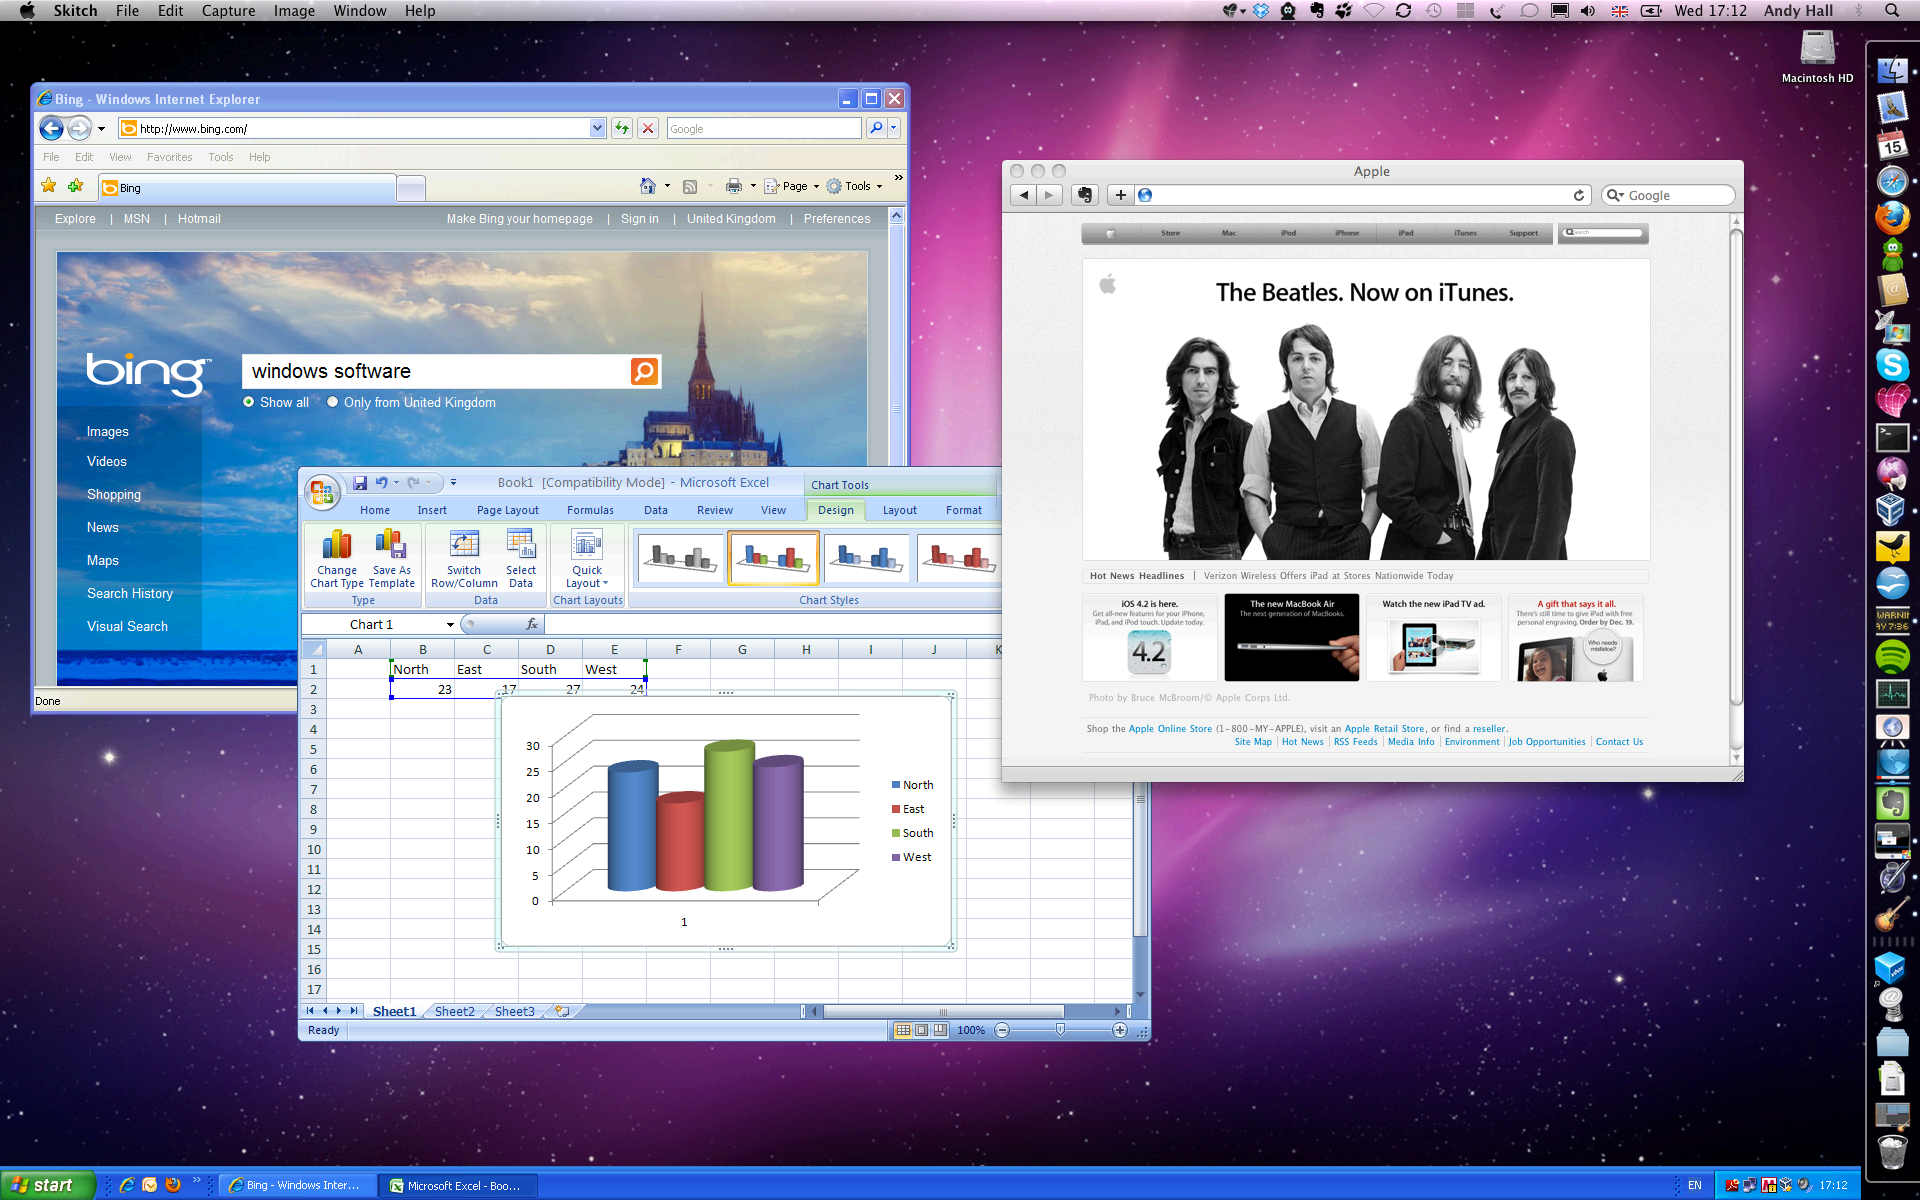
\includegraphics[width=14cm]{images/seamless.png}
\end{center}To enable seamless mode, after starting the virtual
    machine, press the Host key (normally the right control key) together with
    \OQ{}L\CQ{}. This will enlarge the size of the VM's display to the size of your
    host screen and mask out the guest operating system's background. To go
    back to the \OQ{}normal\CQ{} VM display (i.e. to disable seamless windows), press
    the Host key and \OQ{}L\CQ{} again.

\section{Guest properties}
\label{guestadd-guestprops}


Starting with version 2.1, VirtualBox allows for requesting certain
    properties from a running guest, provided that the VirtualBox Guest
    Additions are installed and the VM is running. This is good for two
    things:

\begin{enumerate}


\item 

A number of predefined VM characteristics are automatically
          maintained by VirtualBox and can be retrieved on the host, e.g. to
          monitor VM performance and statistics.


\item 

In addition, arbitrary string data can be exchanged between
          guest and host. This works in both directions.

\end{enumerate}


To accomplish this, VirtualBox establishes a private communication
    channel between the VirtualBox Guest Additions and the host, and software
    on both sides can use this channel to exchange string data for arbitrary
    purposes. Guest properties are simply string keys to which a value is
    attached. They can be set (written to) by either the host and the guest,
    and they can also be read from both sides.

In addition to establishing the general mechanism of reading and
    writing values, a set of predefined guest properties is automatically
    maintained by the VirtualBox Guest Additions to allow for retrieving
    interesting guest data such as the guest's exact operating system and
    service pack level, the installed version of the Guest Additions, users
    that are currently logged into the guest OS, network statistics and more.
    These predefined properties are all prefixed with
    \texttt{/VirtualBox/} and organized into a
    hierarchical tree of keys.

Some of this runtime information is shown when you select \OQ{}Session
    Information Dialog\CQ{} from a virtual machine's \OQ{}Machine\CQ{} menu.

A more flexible way to use this channel is via the
    \texttt{VBoxManage guestproperty} command set; see
    chapter \ref{vboxmanage-guestproperty}, \textit{\nameref{vboxmanage-guestproperty}}, page \pageref{vboxmanage-guestproperty} for details. For example, to
    have \textit{all} the available guest properties for a given
    running VM listed with their respective values, use this:

\begin{Verbatim}[fontsize=\footnotesize]
$ VBoxManage guestproperty enumerate "Windows Vista III"
VirtualBox Command Line Management Interface Version 4.3.28
(C) 2005-2015 Oracle Corporation
All rights reserved.

Name: /VirtualBox/GuestInfo/OS/Product, value: Windows Vista Business Edition,
    timestamp: 1229098278843087000, flags:
Name: /VirtualBox/GuestInfo/OS/Release, value: 6.0.6001,
    timestamp: 1229098278950553000, flags:
Name: /VirtualBox/GuestInfo/OS/ServicePack, value: 1,
    timestamp: 1229098279122627000, flags:
Name: /VirtualBox/GuestAdd/InstallDir,
    value: C:/Program Files/Oracle/VirtualBox
    Guest Additions, timestamp: 1229098279269739000, flags:
Name: /VirtualBox/GuestAdd/Revision, value: 40720,
    timestamp: 1229098279345664000, flags:
Name: /VirtualBox/GuestAdd/Version, value: 4.3.28,
    timestamp: 1229098279479515000, flags:
Name: /VirtualBox/GuestAdd/Components/VBoxControl.exe, value: 4.3.28r40720,
    timestamp: 1229098279651731000, flags:
Name: /VirtualBox/GuestAdd/Components/VBoxHook.dll, value: 4.3.28r40720,
    timestamp: 1229098279804835000, flags:
Name: /VirtualBox/GuestAdd/Components/VBoxDisp.dll, value: 4.3.28r40720,
    timestamp: 1229098279880611000, flags:
Name: /VirtualBox/GuestAdd/Components/VBoxMRXNP.dll, value: 4.3.28r40720,
    timestamp: 1229098279882618000, flags:
Name: /VirtualBox/GuestAdd/Components/VBoxService.exe, value: 4.3.28r40720,
    timestamp: 1229098279883195000, flags:
Name: /VirtualBox/GuestAdd/Components/VBoxTray.exe, value: 4.3.28r40720,
    timestamp: 1229098279885027000, flags:
Name: /VirtualBox/GuestAdd/Components/VBoxGuest.sys, value: 4.3.28r40720,
    timestamp: 1229098279886838000, flags:
Name: /VirtualBox/GuestAdd/Components/VBoxMouse.sys, value: 4.3.28r40720,
    timestamp: 1229098279890600000, flags:
Name: /VirtualBox/GuestAdd/Components/VBoxSF.sys, value: 4.3.28r40720,
    timestamp: 1229098279893056000, flags:
Name: /VirtualBox/GuestAdd/Components/VBoxVideo.sys, value: 4.3.28r40720,
    timestamp: 1229098279895767000, flags:
Name: /VirtualBox/GuestInfo/OS/LoggedInUsers, value: 1,
    timestamp: 1229099826317660000, flags:
Name: /VirtualBox/GuestInfo/OS/NoLoggedInUsers, value: false,
    timestamp: 1229098455580553000, flags:
Name: /VirtualBox/GuestInfo/Net/Count, value: 1,
    timestamp: 1229099826299785000, flags:
Name: /VirtualBox/HostInfo/GUI/LanguageID, value: C,
    timestamp: 1229098151272771000, flags:
Name: /VirtualBox/GuestInfo/Net/0/V4/IP, value: 192.168.2.102,
    timestamp: 1229099826300088000, flags:
Name: /VirtualBox/GuestInfo/Net/0/V4/Broadcast, value: 255.255.255.255,
    timestamp: 1229099826300220000, flags:
Name: /VirtualBox/GuestInfo/Net/0/V4/Netmask, value: 255.255.255.0,
    timestamp: 1229099826300350000, flags:
Name: /VirtualBox/GuestInfo/Net/0/Status, value: Up,
    timestamp: 1229099826300524000, flags:
Name: /VirtualBox/GuestInfo/OS/LoggedInUsersList, value: username,
    timestamp: 1229099826317386000, flags:
\end{Verbatim}


To query the value of a single property, use the \OQ{}get\CQ{} subcommand
    like this:

\begin{Verbatim}[fontsize=\footnotesize]
$ VBoxManage guestproperty get "Windows Vista III" "/VirtualBox/GuestInfo/OS/Product"
VirtualBox Command Line Management Interface Version 4.3.28
(C) 2005-2015 Oracle Corporation
All rights reserved.

Value: Windows Vista Business Edition
\end{Verbatim}


To add or change guest properties from the guest, use the tool
    \texttt{VBoxControl}. This tool is included in the
    Guest Additions of VirtualBox 2.2 or later. When started from a Linux
    guest, this tool requires root privileges for security reasons:

\begin{Verbatim}[fontsize=\footnotesize]
$ sudo VBoxControl guestproperty enumerate
VirtualBox Guest Additions Command Line Management Interface Version 4.3.28
(C) 2009-2015 Oracle Corporation
All rights reserved.

Name: /VirtualBox/GuestInfo/OS/Release, value: 2.6.28-18-generic,
    timestamp: 1265813265835667000, flags: <NULL>
Name: /VirtualBox/GuestInfo/OS/Version, value: #59-Ubuntu SMP Thu Jan 28 01:23:03 UTC 2010,
    timestamp: 1265813265836305000, flags: <NULL>
      ...
\end{Verbatim}


For more complex needs, you can use the VirtualBox programming
    interfaces; see chapter \ref{VirtualBoxAPI}, \textit{\nameref{VirtualBoxAPI}}, page \pageref{VirtualBoxAPI}.

\section{Guest control}
\label{guestadd-guestcontrol}


Starting with version 3.2, the Guest Additions of VirtualBox allow
    starting applications inside a VM from the host system.

For this to work, the application needs to be installed inside the
    guest; no additional software needs to be installed on the host.
    Additionally, text mode output (to stdout and stderr) can be shown on the
    host for further processing along with options to specify user credentials
    and a timeout value (in milliseconds) to limit time the application is
    able to run.

This feature can be used to automate deployment of software within
    the guest.

Starting with version 4.0, the Guest Additions for Windows allow for
    automatic updating (only already installed Guest Additions 4.0 or later).
    Also, copying files from host to the guest as well as remotely creating
    guest directories is available.

To use these features, use the VirtualBox command line, see chapter \ref{vboxmanage-guestcontrol}, \textit{\nameref{vboxmanage-guestcontrol}}, page \pageref{vboxmanage-guestcontrol}.

\section{Memory overcommitment}


In server environments with many VMs; the Guest Additions can be
    used to share physical host memory between several VMs, reducing the total
    amount of memory in use by the VMs. If memory usage is the limiting factor
    and CPU resources are still available, this can help with packing more VMs
    on each host.

\subsection{Memory ballooning}
\label{guestadd-balloon}


Starting with version 3.2, the Guest Additions of VirtualBox can
      change the amount of host memory that a VM uses while the machine is
      running. Because of how this is implemented, this feature is called
      \OQ{}memory ballooning\CQ{}.

\vspace{.2cm}

\begin{center}\fbox{\begin{minipage}[c]{0.9\textwidth}\color{colNote}\textbf{Note:} VirtualBox supports memory ballooning only on 64-bit hosts, and
        it is not supported on Mac OS X hosts.\end{minipage}}\end{center}

\vspace{.2cm}



Normally, to change the amount of memory allocated to a virtual
      machine, one has to shut down the virtual machine entirely and modify
      its settings. With memory ballooning, memory that was allocated for a
      virtual machine can be given to another virtual machine without having
      to shut the machine down.

When memory ballooning is requested, the VirtualBox Guest
      Additions (which run inside the guest) allocate physical memory from the
      guest operating system on the kernel level and lock this memory down in
      the guest. This ensures that the guest will not use that memory any
      longer: no guest applications can allocate it, and the guest kernel will
      not use it either. VirtualBox can then re-use this memory and give it to
      another virtual machine.

The memory made available through the ballooning mechanism is only
      available for re-use by VirtualBox. It is \textit{not}
      returned as free memory to the host. Requesting balloon memory from a
      running guest will therefore not increase the amount of free,
      unallocated memory on the host. Effectively, memory ballooning is
      therefore a memory overcommitment mechanism for multiple virtual
      machines while they are running. This can be useful to temporarily start
      another machine, or in more complicated environments, for sophisticated
      memory management of many virtual machines that may be running in
      parallel depending on how memory is used by the guests.

At this time, memory ballooning is only supported through
      VBoxManage. Use the following command to increase or decrease the size
      of the memory balloon within a running virtual machine that has Guest
      Additions installed: 

\begin{Verbatim}[fontsize=\footnotesize]
VBoxManage controlvm "VM name" guestmemoryballoon <n>
\end{Verbatim}
where
      \texttt{"VM name"} is the name or UUID of the
      virtual machine in question and
      \texttt{<n>} is the amount of memory to
      allocate from the guest in megabytes. See chapter \ref{vboxmanage-controlvm}, \textit{\nameref{vboxmanage-controlvm}}, page \pageref{vboxmanage-controlvm} for more information.

You can also set a default balloon that will automatically be
      requested from the VM every time after it has started up with the
      following command: 

\begin{Verbatim}[fontsize=\footnotesize]
VBoxManage modifyvm "VM name" --guestmemoryballoon <n>
\end{Verbatim}


By default, no balloon memory is allocated. This is a VM setting,
      like other \texttt{modifyvm} settings, and
      therefore can only be set while the machine is shut down; see chapter \ref{vboxmanage-modifyvm}, \textit{\nameref{vboxmanage-modifyvm}}, page \pageref{vboxmanage-modifyvm}.

\subsection{Page Fusion}
\label{guestadd-pagefusion}


Whereas memory ballooning simply reduces the amount of RAM that is
      available to a VM, Page Fusion works differently: it avoids memory
      duplication between several similar running VMs.

In a server environment running several similar VMs (e.g. with
      identical operating systems) on the same host, lots of memory pages are
      identical. VirtualBox's Page Fusion technology, introduced with
      VirtualBox 3.2, is a novel technique to efficiently identify these
      identical memory pages and share them between multiple VMs.

\vspace{.2cm}

\begin{center}\fbox{\begin{minipage}[c]{0.9\textwidth}\color{colNote}\textbf{Note:} VirtualBox supports Page Fusion only on 64-bit hosts, and it
          is not supported on Mac OS X hosts. Page Fusion currently works only
          with Windows guests (2000 and later).\end{minipage}}\end{center}

\vspace{.2cm}



The more similar the VMs on a given host are, the more efficiently
      Page Fusion can reduce the amount of host memory that is in use. It
      therefore works best if all VMs on a host run identical operating
      systems (e.g. Windows XP Service Pack 2). Instead of having a complete
      copy of each operating system in each VM, Page Fusion identifies the
      identical memory pages in use by these operating systems and eliminates
      the duplicates, sharing host memory between several machines
      (\OQ{}deduplication\CQ{}). If a VM tries to modify a page that has been shared
      with other VMs, a new page is allocated again for that VM with a copy of
      the shared page (\OQ{}copy on write\CQ{}). All this is fully transparent to the
      virtual machine.

You may be familiar with this kind of memory overcommitment from
      other hypervisor products, which call this feature \OQ{}page sharing\CQ{} or
      \OQ{}same page merging\CQ{}. However, Page Fusion differs significantly from
      those other solutions, whose approaches have several
      drawbacks:

\begin{enumerate}


\item 

Traditional hypervisors scan \textit{all} guest
            memory and compute checksums (hashes) for every single memory
            page. Then, they look for pages with identical hashes and compare
            the entire content of those pages; if two pages produce the same
            hash, it is very likely that the pages are identical in content.
            This, of course, can take rather long, especially if the system is
            not idling. As a result, the additional memory only becomes
            available after a significant amount of time (this can be hours or
            even days!). Even worse, this kind of page sharing algorithm
            generally consumes significant CPU resources and increases the
            virtualization overhead by 10-20\%.

Page Fusion in VirtualBox uses logic in the VirtualBox Guest
            Additions to quickly identify memory cells that are most likely
            identical across VMs. It can therefore achieve most of the
            possible savings of page sharing almost immediately and with
            almost no overhead.


\item 

Page Fusion is also much less likely to be confused by
            identical memory that it will eliminate just to learn seconds
            later that the memory will now change and having to perform a
            highly expensive and often service-disrupting reallocation.

\end{enumerate}


At this time, Page Fusion can only be controlled with VBoxManage,
      and only while a VM is shut down. To enable Page Fusion for a VM, use
      the following command:

\begin{Verbatim}[fontsize=\footnotesize]
VBoxManage modifyvm "VM name" --pagefusion on
\end{Verbatim}


You can observe Page Fusion operation using some metrics.
      \texttt{RAM/VMM/Shared} shows the total amount
      of fused pages, whereas the per-VM metric
      \texttt{Guest/RAM/Usage/Shared} will return the
      amount of fused memory for a given VM. Please refer to chapter \ref{metrics}, \textit{\nameref{metrics}}, page \pageref{metrics} for information on how to query metrics.

\chapter{Virtual storage}
\label{storage}


As the virtual machine will most probably expect to see a hard disk
  built into its virtual computer, VirtualBox must be able to present \OQ{}real\CQ{}
  storage to the guest as a virtual hard disk. There are presently three
  methods in which to achieve this:

\begin{enumerate}


\item 

Most commonly, VirtualBox will use large image files on a real
      hard disk and present them to a guest as a virtual hard disk. This is
      described in chapter \ref{vdidetails}, \textit{\nameref{vdidetails}}, page \pageref{vdidetails}.


\item 

Alternatively, if you have iSCSI storage servers, you can attach
      such a server to VirtualBox as well; this is described in chapter \ref{storage-iscsi}, \textit{\nameref{storage-iscsi}}, page \pageref{storage-iscsi}.


\item 

Finally, as an advanced feature, you can allow a virtual
      machine to access one of your host disks directly; this advanced feature
      is described in chapter \ref{rawdisk}, \textit{\nameref{rawdisk}}, page \pageref{rawdisk}.

\end{enumerate}


Each such virtual storage device (image file, iSCSI target or physical
  hard disk) will need to be connected to the virtual hard disk controller
  that VirtualBox presents to a virtual machine. This is explained in the next
  section.

\section{Hard disk controllers: IDE, SATA (AHCI), SCSI, SAS}
\label{harddiskcontrollers}


In a real PC, hard disks and CD/DVD drives are connected to a device
    called hard disk controller which drives hard disk operation and data
    transfers. VirtualBox can emulate the four most common types of hard disk
    controllers typically found in today's PCs: IDE, SATA (AHCI), SCSI and
    SAS.\footnote{SATA support was added with VirtualBox 1.6; experimental SCSI
        support was added with 2.1 and fully implemented with 2.2. Generally,
        storage attachments were made much more flexible with VirtualBox 3.1;
        see below. Support for the LSI Logic SAS controller was added with
        VirtualBox 3.2.}

\begin{itemize}


\item 

\textbf{IDE (ATA)} controllers are a
          backwards compatible yet very advanced extension of the disk
	  controller in the IBM PC/AT (1984). Initially, this interface
          worked only with hard disks, but was later extended to also support
          CD-ROM drives and other types of removable media. In physical PCs,
          this standard uses flat ribbon parallel cables with 40 or 80 wires.
          Each such cable can connect two devices to a controller, which have
          traditionally been called \OQ{}master\CQ{} and \OQ{}slave\CQ{}. Typical PCs had
          two connectors for such cables; as a result, support for up to four
	  IDE devices was most common.

In VirtualBox, each virtual machine may have one IDE
          contoller enabled, which gives you up to four virtual storage
          devices that you can attach to the machine. (By default, one of
          these four -- the secondary master -- is preconfigured to be the
          machine's virtual CD/DVD drive, but this can be changed.\footnote{The assignment of the machine's CD/DVD drive to the
              secondary master was fixed before VirtualBox 3.1; it is now
              changeable, and the drive can be at other slots of the IDE
              controller, and there can be more than one such drive.})

So even if your guest operating system has no support for SCSI
          or SATA devices, it should always be able to see an IDE controller.
          

You can also select which exact type of IDE controller
          hardware VirtualBox should present to the virtual machine (PIIX3,
          PIIX4 or ICH6). This makes no difference in terms of performance,
          but if you import a virtual machine from another virtualization
          product, the operating system in that machine may expect a
          particular controller type and crash if it isn't found.

After you have created a new virtual machine with the \OQ{}New
          Virtual Machine\CQ{} wizard of the graphical user interface, you will
          typically see one IDE controller in the machine's \OQ{}Storage\CQ{} settings
          where the virtual CD/DVD drive will be attached to one of the four
          ports of this controller.


\item 

\textbf{Serial ATA (SATA)} is a newer
          standard introduced in 2003. Compared to IDE, it supports both much
          higher speeds and more devices per controller. Also, with
          physical hardware, devices can be added and removed while the system
          is running. The standard interface for SATA controllers is called
          Advanced Host Controller Interface (\textbf{AHCI}).

Like a real SATA controller, VirtualBox's virtual SATA
          controller operates faster and also consumes fewer CPU resources than
          the virtual IDE controller. Also, this allows you to connect up to
          30 virtual hard disks to one machine instead of just three, as with
          the VirtualBox IDE controller (with the DVD drive already attached).

For this reason, starting with version 3.2 and depending on
          the selected guest operating system, VirtualBox uses SATA as the
          default for newly created virtual machines. One virtual SATA
          controller is created by default, and the default disk that is
          created with a new VM is attached to this controller.

\vspace{.2cm}

\begin{center}\fbox{\begin{minipage}[c]{0.9\textwidth}\color{colWarning}\textbf{Warning:} The entire SATA controller and the virtual disks attached
              to it (including those in IDE compatibility mode) will not be
              seen by operating systems that do not have device support for
              AHCI. In particular, \textbf{there is no support
              for AHCI in Windows before Windows Vista}, so Windows
              XP (even SP3) will not see such disks unless you install
              additional drivers. It is possible to switch from IDE to SATA
              after installation by installing the SATA drivers and changing
              the controller type in the VM settings dialog.\footnote{VirtualBox recommends the Intel Matrix Storage drivers
                  which can be downloaded from \url{http://downloadcenter.intel.com/Product\_Filter.aspx?ProductID=2101}.}\end{minipage}}\end{center}

\vspace{.2cm}



To add a SATA controller to a machine for which it has not
          been enabled by default (either because it was created by an earlier
          version of VirtualBox, or because SATA is not supported by default
          by the selected guest operating system), go to the \OQ{}Storage\CQ{} page of
          the machine's settings dialog, click on the \OQ{}Add Controller\CQ{} button
          under the \OQ{}Storage Tree\CQ{} box and then select \OQ{}Add SATA Controller\CQ{}.
          After this, the additional controller will appear as a separate PCI
          device in the virtual machine, and you can add virtual disks to
          it.

To change the IDE compatibility mode settings for the SATA
          controller, please see chapter \ref{vboxmanage-storagectl}, \textit{\nameref{vboxmanage-storagectl}}, page \pageref{vboxmanage-storagectl}.


\item 

\textbf{SCSI} is another established
          industry standard, standing for \OQ{}Small Computer System Interface\CQ{}.
          SCSI was standardized as early as 1986 as a generic interface for
          data transfer between all kinds of devices, including storage
          devices. Today SCSI is still used for connecting hard disks and tape
          devices, but it has mostly been displaced in commodity hardware. It
          is still in common use in high-performance workstations and
          servers.

Primarily for compatibility with other virtualization
          software, VirtualBox optionally supports LSI Logic and BusLogic SCSI
          controllers, to each of which up to 15 virtual hard disks can be
          attached.

To enable a SCSI controller, on the \OQ{}Storage\CQ{} page of a
          virtual machine's settings dialog, click on the \OQ{}Add Controller\CQ{}
          button under the \OQ{}Storage Tree\CQ{} box and then select \OQ{}Add SCSI
          Controller\CQ{}. After this, the additional controller will appear as a
          separate PCI device in the virtual machine.

\vspace{.2cm}

\begin{center}\fbox{\begin{minipage}[c]{0.9\textwidth}\color{colWarning}\textbf{Warning:} As with the other controller types, a SCSI controller will
              only be seen by operating systems with device support for it.
              Windows 2003 and later ships with drivers for the LSI Logic
              controller, while Windows NT 4.0 and Windows 2000 ships with
              drivers for the BusLogic controller. Windows XP ships with
              drivers for neither.\end{minipage}}\end{center}

\vspace{.2cm}




\item 

\textbf{Serial Attached SCSI (SAS)} is
          another bus standard which uses the SCSI command set. As opposed to
          SCSI, however, with physical devices, serial cables are used instead
          of parallel ones, which simplifies physical device connections. In
          some ways, therefore, SAS is to SCSI what SATA is to IDE: it allows
          for more reliable and faster connections.

To support high-end guests which require SAS controllers,
          VirtualBox emulates a LSI Logic SAS controller, which can be enabled
          much the same way as a SCSI controller. At this time, up to eight
          devices can be connected to the SAS controller.

\vspace{.2cm}

\begin{center}\fbox{\begin{minipage}[c]{0.9\textwidth}\color{colWarning}\textbf{Warning:} As with SATA, the SAS controller will only be seen by
            operating systems with device support for it. In particular,
            \textbf{there is no support for SAS in Windows
            before Windows Vista}, so Windows XP (even SP3) will not
            see such disks unless you install additional drivers.\end{minipage}}\end{center}

\vspace{.2cm}



\end{itemize}


In summary, VirtualBox gives you the following categories of virtual
    storage slots:

\begin{enumerate}


\item 

four slots attached to the traditional IDE controller, which
          are always present (one of which typically is a virtual CD/DVD
          drive);


\item 

30 slots attached to the SATA controller, if enabled and
          supported by the guest operating system;


\item 

15 slots attached to the SCSI controller, if enabled and
          supported by the guest operating system;


\item 

eight slots attached to the SAS controller, if enabled and
          supported by the guest operating system.

\end{enumerate}


Given this large choice of storage controllers, you may ask yourself
    which one to choose. In general, you should avoid IDE unless it is the
    only controller supported by your guest. Whether you use SATA, SCSI or SAS
    does not make any real difference. The variety of controllers is only
    supplied for VirtualBox for compatibility with existing hardware and other
    hypervisors.

\section{Disk image files (VDI, VMDK, VHD, HDD)}
\label{vdidetails}


Disk image files reside on the host system and are seen by the guest
    systems as hard disks of a certain geometry. When a guest operating system
    reads from or writes to a hard disk, VirtualBox redirects the request to
    the image file.

Like a physical disk, a virtual disk has a size (capacity), which
    must be specified when the image file is created. As opposed to a physical
    disk however, VirtualBox allows you to expand an image file after
    creation, even if it has data already; see chapter \ref{vboxmanage-modifyvdi}, \textit{\nameref{vboxmanage-modifyvdi}}, page \pageref{vboxmanage-modifyvdi} for details.\footnote{Image resizing was added with VirtualBox 4.0.}

VirtualBox supports four variants of disk image files:

\begin{itemize}


\item 

Normally, VirtualBox uses its own container format for guest
          hard disks -- Virtual Disk Image (VDI) files. In particular, this
          format will be used when you create a new virtual machine with a new
          disk.


\item 

VirtualBox also fully supports the popular and open VMDK
          container format that is used by many other virtualization products,
          in particular, by VMware.\footnote{Initial support for VMDK was added with VirtualBox 1.4;
              since version 2.1, VirtualBox supports VMDK fully, meaning that
              you can create snapshots and use all the other advanced features
              described above for VDI images with VMDK also.}


\item 

VirtualBox also fully supports the VHD format used by
          Microsoft.


\item 

Image files of Parallels version 2 (HDD format) are also
          supported.\footnote{Support was added with VirtualBox 3.1.} For lack of documentation of the format, newer formats
          (3 and 4) are not supported. You can however convert such image
          files to version 2 format using tools provided by Parallels.

\end{itemize}


Irrespective of the disk capacity and format, as briefly mentioned
    in chapter \ref{gui-createvm}, \textit{\nameref{gui-createvm}}, page \pageref{gui-createvm}, there are two options of how to create
    a disk image: fixed-size or dynamically allocated.

\begin{itemize}


\item 

If you create a \textbf{fixed-size
        image}, an image file will be created on your host system
        which has roughly the same size as the virtual disk's capacity. So,
        for a 10G disk, you will have a 10G file. Note that the creation of a
        fixed-size image can take a long time depending on the size of the
        image and the write performance of your hard disk.


\item 

For more flexible storage management, use a \textbf{dynamically allocated image}. This will
        initially be very small and not occupy any space for unused virtual
        disk sectors, but will grow every time a disk sector is written to for
        the first time, until the drive reaches the maximum capacity chosen
        when the drive was created. While this format takes less space
        initially, the fact that VirtualBox needs to expand the image file
        consumes additional computing resources, so until the disk file size has
        stabilized, write operations may be slower than with fixed size disks.
        However, after a time the rate of growth will slow and the average penalty
        for write operations will be negligible.

\end{itemize}


\section{The Virtual Media Manager}
\label{vdis}


VirtualBox keeps track of all the hard disk, CD/DVD-ROM and floppy
    disk images which are in use by virtual machines. These are often referred
    to as \OQ{}known media\CQ{} and come from two sources:

\begin{itemize}


\item 

all media currently attached to virtual machines;


\item 

\OQ{}registered\CQ{} media for compatibility with VirtualBox versions
          older than version 4.0. For details about how media registration has
          changed with version 4.0, please refer to chapter \ref{vboxconfigdata}, \textit{\nameref{vboxconfigdata}}, page \pageref{vboxconfigdata}.

\end{itemize}


The known media can be viewed and changed in the \textbf{Virtual Media Manager}, which you can access from
    the \OQ{}File\CQ{} menu in the VirtualBox main window:

\begin{center}
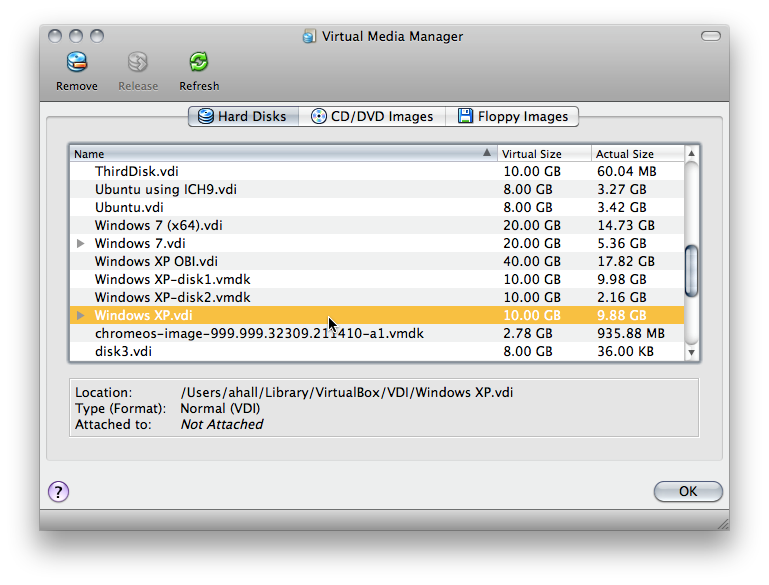
\includegraphics[width=12cm]{images/virtual-disk-manager.png}
\end{center}The known media are conveniently grouped in three tabs for
    the three possible formats. These formats are:

\begin{itemize}


\item 

Hard disk images, either in VirtualBox's own Virtual Disk Image
        (VDI) format or in the third-party formats listed in the previous
        chapter;


\item 

CD/DVD images in standard ISO format;


\item 

floppy images in standard RAW format.

\end{itemize}


As you can see in the screenshot above, for each image, the Virtual
    Media Manager shows you the full path of the image file and other
    information, such as the virtual machine the image is currently attached
    to, if any.

The Virtual Media Manager allows you to

\begin{itemize}


\item 

\textbf{remove} an image from the
        registry (and optionally delete the image file when doing so);


\item 

\textbf{\OQ{}release\CQ{}} an image, that is,
        detach it from a virtual machine if it is currently attached to one as
        a virtual hard disk.

\end{itemize}


Starting with version 4.0, to \textbf{create new disk
    images,} please use the \OQ{}Storage\CQ{} page in a virtual machine's
    settings dialog because disk images are now by default stored in each
    machine's own folder.

Hard disk image files can be copied onto other host systems and
    imported into virtual machines there, although certain guest systems
    (notably Windows 2000 and XP) will require that the new virtual machine be
    set up in a similar way to the old one.

\vspace{.2cm}

\begin{center}\fbox{\begin{minipage}[c]{0.9\textwidth}\color{colNote}\textbf{Note:} Do not simply make copies of virtual disk images. If you import
        such a second copy into a virtual machine, VirtualBox will complain
        with an error, since VirtualBox assigns a unique identifier (UUID) to
        each disk image to make sure it is only used once. See chapter \ref{cloningvdis}, \textit{\nameref{cloningvdis}}, page \pageref{cloningvdis} for instructions on this matter. Also, if you
        want to copy a virtual machine to another system, VirtualBox has an
        import/export facility that might be better suited for your needs; see
        chapter \ref{ovf}, \textit{\nameref{ovf}}, page \pageref{ovf}.\end{minipage}}\end{center}

\vspace{.2cm}



\section{Special image write modes}
\label{hdimagewrites}


For each virtual disk image supported by VirtualBox, you can
    determine separately how it should be affected by write operations from a
    virtual machine and snapshot operations. This applies to all of the
    aforementioned image formats (VDI, VMDK, VHD or HDD) and irrespective of
    whether an image is fixed-size or dynamically allocated.

By default, images are in \OQ{}normal\CQ{} mode. To mark an existing image
    with one of the non-standard modes listed below, use
    \texttt{VBoxManage modifyhd}; see chapter \ref{vboxmanage-modifyvdi}, \textit{\nameref{vboxmanage-modifyvdi}}, page \pageref{vboxmanage-modifyvdi}. Alternatively, use VBoxManage to attach
    the image to a VM and use the \texttt{-{}-mtype}
    argument; see chapter \ref{vboxmanage-storageattach}, \textit{\nameref{vboxmanage-storageattach}}, page \pageref{vboxmanage-storageattach}.

\begin{enumerate}


\item 

With \textbf{normal images} (the default
        setting), there are no restrictions on how guests can read from and
        write to the disk.

When you take a snapshot of your virtual machine as described in
        chapter \ref{snapshots}, \textit{\nameref{snapshots}}, page \pageref{snapshots}, the state of such a \OQ{}normal hard disk\CQ{}
        will be recorded together with the snapshot, and when reverting to the
        snapshot, its state will be fully reset.

(Technically, strictly speaking, the image file itself is not
        \OQ{}reset\CQ{}. Instead, when a snapshot is taken, VirtualBox \OQ{}freezes\CQ{} the
        image file and no longer writes to it. For the write operations from
        the VM, a second, \OQ{}differencing\CQ{} image file is created which receives
        only the changes to the original image; see the next section for
        details.)

While you can attach the same \OQ{}normal\CQ{} image to more than one
        virtual machine, only one of these virtual machines attached to the
        same image file can be executed simultaneously, as otherwise there
        would be conflicts if several machines write to the same image
        file.\footnote{This restriction is more lenient now than it was before
            VirtualBox 2.2. Previously, each \OQ{}normal\CQ{} disk image could only be
            \textit{attached} to one single machine. Now it can be
            attached to more than one machine so long as only one of these
            machines is running.}


\item 

By contrast, \textbf{write-through hard
        disks} are completely unaffected by snapshots: their state
        is \textit{not} saved when a snapshot is taken, and not
        restored when a snapshot is restored.


\item 

\textbf{Shareable hard disks} are a
        variant of write-through hard disks. In principle they behave exactly
        the same, i.e. their state is \textit{not} saved when a
        snapshot is taken, and not restored when a snapshot is restored. The
        difference only shows if you attach such disks to several VMs.
        Shareable disks may be attached to several VMs which may run
        concurrently. This makes them suitable for use by cluster filesystems
        between VMs and similar applications which are explicitly prepared to
        access a disk concurrently. Only fixed size images can be used in this
        way, and dynamically allocated images are rejected.

\vspace{.2cm}

\begin{center}\fbox{\begin{minipage}[c]{0.9\textwidth}\color{colWarning}\textbf{Warning:} This is an expert feature, and misuse can lead to data loss
            -- regular filesystems are not prepared to handle simultaneous
            changes by several parties.\end{minipage}}\end{center}

\vspace{.2cm}




\item 

Next, \textbf{immutable images} only
        remember write accesses temporarily while the virtual machine is
        running; all changes are lost when the virtual machine is powered on
        the next time. As a result, as opposed to \OQ{}normal\CQ{} images, the same
        immutable image can be used with several virtual machines without
        restrictions.

\textit{Creating} an immutable image makes little
        sense since it would be initially empty and lose its contents with
        every machine restart (unless you really want to have a disk that is
        always unformatted when the machine starts up). As a result, normally,
        you would first create a \OQ{}normal\CQ{} image and then, when you deem its
        contents useful, later mark it immutable.

If you take a snapshot of a machine with immutable images, then
        on every machine power-up, those images are reset to the state of the
        last (current) snapshot (instead of the state of the original
        immutable image).

\vspace{.2cm}

\begin{center}\fbox{\begin{minipage}[c]{0.9\textwidth}\color{colNote}\textbf{Note:} As a special exception, immutable images are
          \textit{not} reset if they are attached to a machine
          whose last snapshot was taken while the machine was running (a
          so-called \OQ{}online\CQ{} snapshot). As a result, if the machine's current
          snapshot is such an \OQ{}online\CQ{} snapshot, its immutable images behave
          exactly like the \OQ{}normal\CQ{} images described previously. To re-enable
          the automatic resetting of such images, delete the current snapshot
          of the machine.\end{minipage}}\end{center}

\vspace{.2cm}



Again, technically, VirtualBox never writes to an immutable
        image directly at all. All write operations from the machine will be
        directed to a differencing image; the next time the VM is powered on,
        the differencing image is reset so that every time the VM starts, its
        immutable images have exactly the same content.\footnote{This behavior also changed with VirtualBox 2.2. Previously,
            the differencing images were discarded when the machine session
            \textit{ended}; now they are discarded every time the
            machine is powered on.} The differencing image is only reset when the machine is
        powered on from within VirtualBox, not when you reboot by requesting a
        reboot from within the machine. This is also why immutable images
        behave as described above when snapshots are also present, which use
        differencing images as well.

If the automatic discarding of the differencing image on VM
        startup does not fit your needs, you can turn it off using the
        \texttt{autoreset} parameter of
        \texttt{VBoxManage modifyhd}; see chapter \ref{vboxmanage-modifyvdi}, \textit{\nameref{vboxmanage-modifyvdi}}, page \pageref{vboxmanage-modifyvdi} for details.


\item 

An image in \textbf{multiattach mode}
        can be attached to more than one virtual machine at the same time,
        even if these machines are running simultaneously. For each virtual
        machine to which such an image is attached, a differencing image is
        created. As a result, data that is written to such a virtual disk by
        one machine is not seen by the other machines to which the image is
        attached; each machine creates its own write history of the
        multiattach image.

Technically, a \OQ{}multiattach\CQ{} image behaves identically to an
        \OQ{}immutable\CQ{} image except the differencing image is not reset every
        time the machine starts.

This mode is useful for sharing files which are almost never
        written, for instance picture galleries, where every guest changes
        only a small amount of data and the majority of the disk content
        remains unchanged. The modified blocks are stored in differencing
        images which remain reletively small and the shared content is stored
        only once at the host.


\item 

Finally, the \textbf{read-only image} is
        used automatically for CD/DVD images, since CDs/DVDs can never be
        written to.

\end{enumerate}


To illustrate the differences between the various types with respect
    to snapshots: Assume you have installed your guest operating system in
    your VM, and you have taken a snapshot. Imagine you have accidentally
    infected your VM with a virus and would like to go back to the snapshot.
    With a normal hard disk image, you simply restore the snapshot, and the
    earlier state of your hard disk image will be restored as well (and your
    virus infection will be undone). With an immutable hard disk, all it takes
    is to shut down and power on your VM, and the virus infection will be
    discarded. With a write-through image however, you cannot easily undo the
    virus infection by means of virtualization, but will have to disinfect
    your virtual machine like a real computer.

Still, you might find write-through images useful if you want to
    preserve critical data irrespective of snapshots, and since you can attach
    more than one image to a VM, you may want to have one immutable for the
    operating system and one write-through for your data files.

\section{Differencing images}
\label{diffimages}


The previous section hinted at differencing images and how they are
    used with snapshots, immutable images and multiple disk attachments. For
    the inquisitive VirtualBox user, this section describes in more detail how
    they work.

A differencing image is a special disk image that only holds the
    differences to another image. A differencing image by itself is useless,
    it must always refer to another image. The differencing image is then
    typically referred to as a \OQ{}child\CQ{}, which holds the differences to its
    \OQ{}parent\CQ{}.

When a differencing image is active, it receives all write
    operations from the virtual machine instead of its parent. The
    differencing image only contains the sectors of the virtual hard disk that
    have changed since the differencing image was created. When the machine
    reads a sector from such a virtual hard disk, it looks into the
    differencing image first. If the sector is present, it is returned from
    there; if not, VirtualBox looks into the parent. In other words, the
    parent becomes \OQ{}read-only\CQ{}; it is never written to again, but it is read
    from if a sector has not changed.

Differencing images can be chained. If another differencing image is
    created for a virtual disk that already has a differencing image, then it
    becomes a \OQ{}grandchild\CQ{} of the original parent. The first differencing
    image then becomes read-only as well, and write operations only go to the
    second-level differencing image. When reading from the virtual disk,
    VirtualBox needs to look into the second differencing image first, then
    into the first if the sector was not found, and then into the original
    image.

There can be an unlimited number of differencing images, and each
    image can have more than one child. As a result, the differencing images
    can form a complex tree with parents, \OQ{}siblings\CQ{} and children, depending
    on how complex your machine configuration is. Write operations always go
    to the one \OQ{}active\CQ{} differencing image that is attached to the machine,
    and for read operations, VirtualBox may need to look up all the parents in
    the chain until the sector in question is found. You can look at such a
    tree in the Virtual Media Manager:\begin{center}
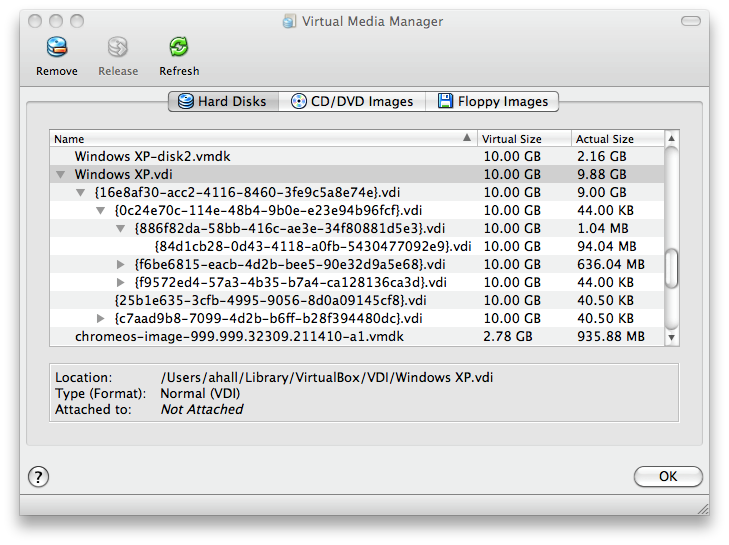
\includegraphics[width=12cm]{images/virtual-disk-manager2.png}
\end{center}

In all of these situations, from the point of view of the virtual
    machine, the virtual hard disk behaves like any other disk. While the
    virtual machine is running, there is a slight run-time I/O overhead
    because VirtualBox might need to look up sectors several times. This is
    not noticeable however since the tables with sector information are always
    kept in memory and can be looked up quickly.

Differencing images are used in the following
    situations:

\begin{enumerate}


\item 

\textbf{Snapshots.} When you create a
          snapshot, as explained in the previous section, VirtualBox \OQ{}freezes\CQ{}
          the images attached to the virtual machine and creates differencing
          images for each of them (to be precise: one for each image that is
          not in \OQ{}write-through\CQ{} mode). From the point of view of the virtual
          machine, the virtual disks continue to operate before, but all write
          operations go into the differencing images. Each time you create
          another snapshot, for each hard disk attachment, another
          differencing image is created and attached, forming a chain or
          tree.

In the above screenshot, you see that the original disk image
          is now attached to a snapshot, representing the state of the disk
          when the snapshot was taken.

If you now \textbf{restore} a snapshot
          -- that is, if you want to go back to the exact machine state that
          was stored in the snapshot --, the following happens:

\begin{enumerate}


\item 

VirtualBox copies the virtual machine settings that were
                copied into the snapshot back to the virtual machine. As a
                result, if you have made changes to the machine configuration
                since taking the snapshot, they are undone.


\item 

If the snapshot was taken while the machine was running,
                it contains a saved machine state, and that state is restored
                as well; after restoring the snapshot, the machine will then
                be in \OQ{}Saved\CQ{} state and resume execution from there when it is
                next started. Otherwise the machine will be in \OQ{}Powered Off\CQ{}
                state and do a full boot.


\item 

For each disk image attached to the machine, the
                differencing image holding all the write operations since the
                current snapshot was taken is thrown away, and the original
                parent image is made active again. (If you restored the \OQ{}root\CQ{}
                snapshot, then this will be the root disk image for each
                attachment; otherwise, some other differencing image descended
                from it.) This effectively restores the old machine
                state.

\end{enumerate}


If you later \textbf{delete} a
          snapshot in order to free disk space, for each disk attachment, one
          of the differencing images becomes obsolete. In this case, the
          differencing image of the disk attachment cannot simply be deleted.
          Instead, VirtualBox needs to look at each sector of the differencing
          image and needs to copy it back into its parent; this is called
          \OQ{}merging\CQ{} images and can be a potentially lengthy process, depending
          on how large the differencing image is. It can also temporarily need
          a considerable amount of extra disk space, before the differencing
          image obsoleted by the merge operation is deleted.


\item 

\textbf{Immutable images.} When an
          image is switched to \OQ{}immutable\CQ{} mode, a differencing image is
          created as well. As with snapshots, the parent image then becomes
          read-only, and the differencing image receives all the write
          operations. Every time the virtual machine is started, all the
          immutable images which are attached to it have their respective
          differencing image thrown away, effectively resetting the virtual
          machine's virtual disk with every restart.

\end{enumerate}


\section{Cloning disk images}
\label{cloningvdis}


You can duplicate hard disk image files on the same host to quickly
    produce a second virtual machine with the same operating system setup.
    However, you should \textit{only} make copies of virtual disk
    images using the utility supplied with VirtualBox; see chapter \ref{vboxmanage-clonevdi}, \textit{\nameref{vboxmanage-clonevdi}}, page \pageref{vboxmanage-clonevdi}. This is because VirtualBox assigns a
    unique identity number (UUID) to each disk image, which is also stored
    inside the image, and VirtualBox will refuse to work with two images that
    use the same number. If you do accidentally try to reimport a disk image
    which you copied normally, you can make a second copy using VirtualBox's
    utility and import that instead.

Note that newer Linux distributions identify the boot hard disk from
    the ID of the drive. The ID VirtualBox reports for a drive is determined
    from the UUID of the virtual disk image. So if you clone a disk image and
    try to boot the copied image the guest might not be able to determine its
    own boot disk as the UUID changed. In this case you have to adapt the disk
    ID in your boot loader script (for example
    \texttt{/boot/grub/menu.lst}). The disk ID looks
    like this:

\begin{Verbatim}[fontsize=\footnotesize]
scsi-SATA_VBOX_HARDDISK_VB5cfdb1e2-c251e503
\end{Verbatim}


The ID for the copied image can be determined with 

\begin{Verbatim}[fontsize=\footnotesize]
hdparm -i /dev/sda
\end{Verbatim}


\section{Host I/O caching}
\label{iocaching}


Starting with version 3.2, VirtualBox can optionally disable the I/O
    caching that the host operating system would otherwise perform on disk
    image files.

Traditionally, VirtualBox has opened disk image files as normal
    files, which results in them being cached by the host operating system
    like any other file. The main advantage of this is speed: when the guest
    OS writes to disk and the host OS cache uses delayed writing, the write
    operation can be reported as completed to the guest OS quickly while the
    host OS can perform the operation asynchronously. Also, when you start a
    VM a second time and have enough memory available for the OS to use for
    caching, large parts of the virtual disk may be in system memory, and the
    VM can access the data much faster.

Note that this applies only to image files; buffering never occurred
    for virtual disks residing on remote iSCSI storage, which is the more common
    scenario in enterprise-class setups (see chapter \ref{storage-iscsi}, \textit{\nameref{storage-iscsi}}, page \pageref{storage-iscsi}).

While buffering is a useful default setting for virtualizating a few
    machines on a desktop computer, there are some disadvantages to this
    approach:

\begin{enumerate}


\item 

Delayed writing through the host OS cache is less secure. When
          the guest OS writes data, it considers the data written even though
          it has not yet arrived on a physical disk. If for some reason the
          write does not happen (power failure, host crash), the likelihood of
          data loss increases.


\item 

Disk image files tend to be very large. Caching them can
          therefore quickly use up the entire host OS cache. Depending on the
          efficiency of the host OS caching, this may slow down the host
          immensely, especially if several VMs run at the same time. For
          example, on Linux hosts, host caching may result in Linux delaying
          all writes until the host cache is nearly full and then writing out
          all these changes at once, possibly stalling VM execution for
          minutes. This can result in I/O errors in the guest as I/O requests
          time out there.


\item 

Physical memory is often wasted as guest operating systems
          typically have their own I/O caches, which may result in the data
          being cached twice (in both the guest and the host caches) for
          little effect.

\end{enumerate}


If you decide to disable host I/O caching for the above reasons,
    VirtualBox uses its own small cache to buffer writes, but no read caching
    since this is typically already performed by the guest OS. In addition,
    VirtualBox fully supports asynchronous I/O for its virtual SATA, SCSI and
    SAS controllers through multiple I/O threads.

Since asynchronous I/O is not supported by IDE controllers, for
    performance reasons, you may want to leave host caching enabled for your
    VM's virtual IDE controllers.

For this reason, VirtualBox allows you to configure whether the host
    I/O cache is used for each I/O controller separately. Either uncheck the
    \OQ{}Use host I/O cache\CQ{} box in the \OQ{}Storage\CQ{} settings for a given virtual
    storage controller, or use the following VBoxManage command to disable the
    host I/O cache for a virtual storage controller:

\begin{Verbatim}[fontsize=\footnotesize]
VBoxManage storagectl "VM name" --name <controllername> --hostiocache off
\end{Verbatim}


See chapter \ref{vboxmanage-storagectl}, \textit{\nameref{vboxmanage-storagectl}}, page \pageref{vboxmanage-storagectl} for details.

For the above reasons also, VirtualBox now uses SATA controllers by
    default for new virtual machines.

\section{Limiting bandwidth for disk images}
\label{storage-bandwidth-limit}


Starting with version 4.0, VirtualBox allows for limiting the
    maximum bandwidth used for asynchronous I/O. Additionally it supports
    sharing limits through bandwidth groups for several images. It is possible
    to have more than one such limit.

Limits are configured through
    \texttt{VBoxManage}. The example below creates a
    bandwidth group named \OQ{}Limit\CQ{}, sets the limit to 20 MB/s and assigns the
    group to the attached disks of the VM:

\begin{Verbatim}[fontsize=\footnotesize]
VBoxManage bandwidthctl "VM name" add Limit --type disk --limit 20M
VBoxManage storageattach "VM name" --storagectl "SATA" --port 0 --device 0 --type hdd
                                   --medium disk1.vdi --bandwidthgroup Limit
VBoxManage storageattach "VM name" --storagectl "SATA" --port 1 --device 0 --type hdd
                                   --medium disk2.vdi --bandwidthgroup Limit
\end{Verbatim}


All disks in a group share the bandwidth limit, meaning that in the
    example above the bandwidth of both images combined can never exceed 20
    MB/s. However, if one disk doesn't require bandwidth the other can use the
    remaining bandwidth of its group.

The limits for each group can be changed while the VM is running,
    with changes being picked up immediately. The example below changes the
    limit for the group created in the example above to 10 MB/s:

\begin{Verbatim}[fontsize=\footnotesize]
VBoxManage bandwidthctl "VM name" set Limit --limit 10M
\end{Verbatim}


\section{CD/DVD support}
\label{storage-cds}


The virtual CD/DVD drive(s) by default support only reading. The
    medium configuration is changeable at runtime. You can select between
    three options to provide the medium data:

\begin{itemize}


\item 

\textbf{Host Drive} defines that the
          guest can read from the medium in the host drive.


\item 

\textbf{Image file} (typically an ISO
          file) gives the guest read-only access to the data in the
          image.


\item 

\textbf{Empty} stands for a drive
          without an inserted medium.

\end{itemize}


Changing between the above, or changing a medium in the host drive
    that is accessed by a machine, or changing an image file will signal a
    medium change to the guest operating system, which can then react to the
    change (e.g. by starting an installation program).

Medium changes can be prevented by the guest, and VirtualBox
    reflects that by locking the host drive if appropriate. You can force a
    medium removal in such situations via the VirtualBox GUI or the VBoxManage
    command line tool. Effectively this is the equivalent of the emergency
    eject which many CD/DVD drives provide, with all associated side effects:
    the guest OS can issue error messages, just like on real hardware, and
    guest applications may misbehave. Use this with caution.

\vspace{.2cm}

\begin{center}\fbox{\begin{minipage}[c]{0.9\textwidth}\color{colNote}\textbf{Note:} The identification string of the drive provided to the guest
        (which, in the guest, would be displayed by configuration tools such
        as the Windows Device Manager) is always \OQ{}VBOX CD-ROM\CQ{}, irrespective
        of the current configuration of the virtual drive. This is to prevent
        hardware detection from being triggered in the guest operating system
        every time the configuration is changed.\end{minipage}}\end{center}

\vspace{.2cm}



The standard CD/DVD emulation allows for reading standard data CD
    and DVD formats only. As an experimental feature, for additional
    capabilities, it is possible to give the guest direct access to the CD/DVD
    host drive by enabling \OQ{}passthrough\CQ{} mode. Depending on the host hardware,
    this may enable three things to work, potentially:

\begin{itemize}


\item 

CD/DVD writing from within the guest, if the host DVD drive is
          a CD/DVD writer;


\item 

playing audio CDs;


\item 

playing encrypted DVDs.

\end{itemize}


There is a \OQ{}Passthrough\CQ{} checkbox in the GUI dialog for configuring
    the media attached to a storage controller, or you can use the
    \texttt{-{}-passthrough} option with
    \texttt{VBoxManage storageattach}; see chapter \ref{vboxmanage-storageattach}, \textit{\nameref{vboxmanage-storageattach}}, page \pageref{vboxmanage-storageattach} for details.

Even if pass-through is enabled, unsafe commands, such as updating
    the drive firmware, will be blocked. Video CD formats are never supported,
    not even in passthrough mode, and cannot be played from a virtual
    machine.

On Solaris hosts, pass-through requires running VirtualBox with real
    root permissions due to security measures enforced by the host.

\section{iSCSI servers}
\label{storage-iscsi}


iSCSI stands for \OQ{}Internet SCSI\CQ{} and is a standard that allows for
    using the SCSI protocol over Internet (TCP/IP) connections. Especially
    with the advent of Gigabit Ethernet, it has become affordable to attach
    iSCSI storage servers simply as remote hard disks to a computer network.
    In iSCSI terminology, the server providing storage resources is called an
    \OQ{}iSCSI target\CQ{}, while the client connecting to the server and accessing
    its resources is called \OQ{}iSCSI initiator\CQ{}.

VirtualBox can transparently present iSCSI remote storage to a
    virtual machine as a virtual hard disk. The guest operating system will
    not see any difference between a virtual disk image (VDI file) and an
    iSCSI target. To achieve this, VirtualBox has an integrated iSCSI
    initiator.

VirtualBox's iSCSI support has been developed according to the iSCSI
    standard and should work with all standard-conforming iSCSI targets. To
    use an iSCSI target with VirtualBox, you must use the command line; see
    chapter \ref{vboxmanage-storageattach}, \textit{\nameref{vboxmanage-storageattach}}, page \pageref{vboxmanage-storageattach}.

\chapter{Virtual networking}
\label{networkingdetails}


As briefly mentioned in chapter \ref{settings-network}, \textit{\nameref{settings-network}}, page \pageref{settings-network},
  VirtualBox provides up to eight virtual PCI Ethernet cards for each virtual
  machine. For each such card, you can individually select

\begin{enumerate}


\item 

the hardware that will be virtualized as well as


\item 

the virtualization mode that the virtual card will be operating
        in with respect to your physical networking hardware on the
        host.

\end{enumerate}


Four of the network cards can be configured in the \OQ{}Network\CQ{} section
  of the settings dialog in the graphical user interface of VirtualBox. You
  can configure all eight network cards on the command line via VBoxManage
  modifyvm; see chapter \ref{vboxmanage-modifyvm}, \textit{\nameref{vboxmanage-modifyvm}}, page \pageref{vboxmanage-modifyvm}.

This chapter explains the various networking settings in more
  detail.

\section{Virtual networking hardware}
\label{nichardware}


For each card, you can individually select what kind of
    \textit{hardware} will be presented to the virtual machine.
    VirtualBox can virtualize the following six types of networking
    hardware:

\begin{itemize}


\item 

AMD PCNet PCI II (Am79C970A);


\item 

AMD PCNet FAST III (Am79C973, the default);


\item 

Intel PRO/1000 MT Desktop (82540EM);


\item 

Intel PRO/1000 T Server (82543GC);


\item 

Intel PRO/1000 MT Server (82545EM);


\item 

Paravirtualized network adapter (virtio-net).

\end{itemize}


The PCNet FAST III is the default because it is supported by nearly
    all operating systems out of the box, as well as the GNU GRUB boot
    manager. As an exception, the Intel PRO/1000 family adapters are chosen
    for some guest operating system types that no longer ship with drivers for
    the PCNet card, such as Windows Vista.

The Intel PRO/1000 MT Desktop type works with Windows Vista and
    later versions. The T Server variant of the Intel PRO/1000 card is
    recognized by Windows XP guests without additional driver installation.
    The MT Server variant facilitates OVF imports from other platforms.

The \textbf{\OQ{}Paravirtualized network adapter
    (virtio-net)\OQ{}} is special. If you select this, then VirtualBox
    does \textit{not} virtualize common networking hardware (that
    is supported by common guest operating systems out of the box). Instead,
    VirtualBox then expects a special software interface for virtualized
    environments to be provided by the guest, thus avoiding the complexity of
    emulating networking hardware and improving network performance. Starting
    with version 3.1, VirtualBox provides support for the industry-standard
    \OQ{}virtio\CQ{} networking drivers, which are part of the open-source KVM
    project.

The \OQ{}virtio\CQ{} networking drivers are available for the following
    guest operating systems:



\begin{itemize}


\item 

Linux kernels version 2.6.25 or later can be configured to
          provide virtio support; some distributions also back-ported virtio
          to older kernels.


\item 

For Windows 2000, XP and Vista, virtio drivers can be
          downloaded and installed from the KVM project web page.\footnote{\url{http://www.linux-kvm.org/page/WindowsGuestDrivers}.}

\end{itemize}


VirtualBox also has limited support for so-called \textbf{jumbo frames}, i.e. networking packets with more
    than 1500 bytes of data, provided that you use the Intel card
    virtualization and bridged networking. In other words, jumbo frames are
    not supported with the AMD networking devices; in those cases, jumbo
    packets will silently be dropped for both the transmit and the receive
    direction. Guest operating systems trying to use this feature will observe
    this as a packet loss, which may lead to unexpected application behavior
    in the guest. This does not cause problems with guest operating systems in
    their default configuration, as jumbo frames need to be explicitly
    enabled.

\section{Introduction to networking modes}
\label{networkingmodes}


Each of the eight networking adapters can be separately configured
    to operate in one of the following modes:

\begin{description}


\item[Not attached]

In this mode, VirtualBox reports to the guest that a network
            card is present, but that there is no connection -- as if no
            Ethernet cable was plugged into the card. This way it is possible
            to \OQ{}pull\CQ{} the virtual Ethernet cable and disrupt the connection,
            which can be useful to inform a guest operating system that no
            network connection is available and enforce a
            reconfiguration.

\item[Network Address Translation (NAT)]

If all you want is to browse the Web, download files and
            view e-mail inside the guest, then this default mode should be
            sufficient for you, and you can safely skip the rest of this
            section. Please note that there are certain limitations when using
            Windows file sharing (see chapter \ref{nat-limitations}, \textit{\nameref{nat-limitations}}, page \pageref{nat-limitations} for
            details).

\item[NAT Network]

The NAT network is a new NAT flavour introduced in
              VirtualBox 4.3. See
              chapter \ref{network_nat_service}, \textit{\nameref{network_nat_service}}, page \pageref{network_nat_service}
              for details.

\item[Bridged networking]

This is for more advanced networking needs such as network
            simulations and running servers in a guest. When enabled,
            VirtualBox connects to one of your installed network cards and
            exchanges network packets directly, circumventing your host
            operating system's network stack.

\item[Internal networking]

This can be used to create a different kind of
            software-based network which is visible to selected virtual
            machines, but not to applications running on the host or to the
            outside world.

\item[Host-only networking]

This can be used to create a network containing the host and
            a set of virtual machines, without the need for the host's
            physical network interface. Instead, a virtual network interface
            (similar to a loopback interface) is created on the host,
            providing connectivity among virtual machines and the host.

\item[Generic networking]

Rarely used modes share the same generic network interface,
            by allowing the user to select a driver which can be included with
            VirtualBox or be distributed in an extension pack.

At the moment there are potentially two available
            sub-modes:



\begin{description}


\item[UDP Tunnel]

This can be used to interconnect virtual machines
                    running on different hosts directly, easily and
                    transparently, over existing network
                    infrastructure.

\item[VDE (Virtual Distributed Ethernet)
                  networking]

This option can be used to connect to a Virtual
                    Distributed Ethernet switch on a Linux or a FreeBSD host.
                    At the moment this needs compiling VirtualBox from
                    sources, as the Oracle packages do not include it.
\end{description}

\end{description}


The following sections describe the available network modes in more
    detail.

\section{Network Address Translation (NAT)}
\label{network_nat}


Network Address Translation (NAT) is the simplest way of accessing
    an external network from a virtual machine. Usually, it does not require
    any configuration on the host network and guest system. For this reason,
    it is the default networking mode in VirtualBox.

A virtual machine with NAT enabled acts much like a real computer
    that connects to the Internet through a router. The \OQ{}router\CQ{}, in this
    case, is the VirtualBox networking engine, which maps traffic from and to
    the virtual machine transparently. In VirtualBox this router is placed
    between each virtual machine and the host. This separation maximizes
    security since by default virtual machines cannot talk to each
    other.

The disadvantage of NAT mode is that, much like a private network
    behind a router, the virtual machine is invisible and unreachable from the
    outside internet; you cannot run a server this way unless you set up port
    forwarding (described below).

The network frames sent out by the guest operating system are
    received by VirtualBox's NAT engine, which extracts the TCP/IP data and
    resends it using the host operating system. To an application on the host,
    or to another computer on the same network as the host, it looks like the
    data was sent by the VirtualBox application on the host, using an IP
    address belonging to the host. VirtualBox listens for replies to the
    packages sent, and repacks and resends them to the guest machine on its
    private network.

The virtual machine receives its network address and configuration
    on the private network from a DHCP server integrated into VirtualBox. The
    IP address thus assigned to the virtual machine is usually on a completely
    different network than the host. As more than one card of a virtual
    machine can be set up to use NAT, the first card is connected to the
    private network 10.0.2.0, the second card to the network 10.0.3.0 and so
    on. If you need to change the guest-assigned IP range for some reason,
    please refer to chapter \ref{changenat}, \textit{\nameref{changenat}}, page \pageref{changenat}.

\subsection{Configuring port forwarding with NAT}
\label{natforward}


As the virtual machine is connected to a private network internal
      to VirtualBox and invisible to the host, network services on the guest
      are not accessible to the host machine or to other computers on the same
      network. However, like a physical router, VirtualBox can make selected
      services available to the world outside the guest through \textbf{port forwarding.} This means that VirtualBox
      listens to certain ports on the host and resends all packets which
      arrive there to the guest, on the same or a different port.

To an application on the host or other physical (or virtual)
      machines on the network, it looks as though the service being proxied is
      actually running on the host. This also means that you cannot run the
      same service on the same ports on the host. However, you still gain the
      advantages of running the service in a virtual machine -- for example,
      services on the host machine or on other virtual machines cannot be
      compromised or crashed by a vulnerability or a bug in the service, and
      the service can run in a different operating system than the host
      system.

To configure Port Forwarding you can use the graphical Port
      Forwarding editor which can be found in the Network Settings dialog
      for Network Adaptors configured to use NAT. Here you can map host
      ports to guest ports to allow network traffic to be routed to a
      specific port in the guest.

Alternatively command line tool \texttt{VBoxManage} could be used;
      for details, please refer to chapter \ref{vboxmanage-modifyvm}, \textit{\nameref{vboxmanage-modifyvm}}, page \pageref{vboxmanage-modifyvm}.

You will need to know which ports on the guest the service uses
      and to decide which ports to use on the host (often but not always you
      will want to use the same ports on the guest and on the host). You can
      use any ports on the host which are not already in use by a service. For
      example, to set up incoming NAT connections to an
      \texttt{ssh} server in the guest, use the
      following command: 

\begin{Verbatim}[fontsize=\footnotesize]
VBoxManage modifyvm "VM name" --natpf1 "guestssh,tcp,,2222,,22"
\end{Verbatim}
With
      the above example, all TCP traffic arriving on port 2222 on any host
      interface will be forwarded to port 22 in the guest. The protocol name
      \texttt{tcp} is a mandatory attribute defining
      which protocol should be used for forwarding
      (\texttt{udp} could also be used). The name
      \texttt{guestssh} is purely descriptive and will
      be auto-generated if omitted. The number after
      \texttt{-{}-natpf} denotes the network card, like
      in other parts of VBoxManage.

To remove this forwarding rule again, use the following command:
      

\begin{Verbatim}[fontsize=\footnotesize]
VBoxManage modifyvm "VM name" --natpf1 delete "guestssh"
\end{Verbatim}


If for some reason the guest uses a static assigned IP address not
      leased from the built-in DHCP server, it is required to specify the
      guest IP when registering the forwarding rule: 

\begin{Verbatim}[fontsize=\footnotesize]
VBoxManage modifyvm "VM name" --natpf1 "guestssh,tcp,,2222,10.0.2.19,22"
\end{Verbatim}
This
      example is identical to the previous one, except that the NAT engine is
      being told that the guest can be found at the 10.0.2.19 address.

To forward \textit{all} incoming traffic from a
      specific host interface to the guest, specify the IP of that host
      interface like this:

\begin{Verbatim}[fontsize=\footnotesize]
VBoxManage modifyvm "VM name" --natpf1 "guestssh,tcp,127.0.0.1,2222,,22"
\end{Verbatim}
This
      forwards all TCP traffic arriving on the localhost interface (127.0.0.1)
      via port 2222 to port 22 in the guest.

It is possible to configure incoming NAT connections while the
      VM is running, see chapter \ref{vboxmanage-controlvm}, \textit{\nameref{vboxmanage-controlvm}}, page \pageref{vboxmanage-controlvm}.

\subsection{PXE booting with NAT}
\label{nat-tftp}


PXE booting is now supported in NAT mode. The NAT DHCP server
      provides a boot file name of the form
      \texttt{vmname.pxe} if the directory
      \texttt{TFTP} exists in the directory where the
      user's \texttt{VirtualBox.xml} file is kept. It
      is the responsibility of the user to provide
      \texttt{vmname.pxe}.

\subsection{NAT limitations}
\label{nat-limitations}


There are four \textbf{limitations} of NAT
      mode which users should be aware of:

\begin{description}


\item[ICMP protocol limitations:]

Some frequently used network debugging tools (e.g.
            \texttt{ping} or tracerouting) rely on the
            ICMP protocol for sending/receiving messages. While ICMP support
            has been improved with VirtualBox 2.1
            (\texttt{ping} should now work), some
            other tools may not work reliably.

\item[Receiving of UDP broadcasts is not reliable:]

The guest does not reliably receive broadcasts, since, in
            order to save resources, it only listens for a certain amount of
            time after the guest has sent UDP data on a particular port. As a
            consequence, NetBios name resolution based on broadcasts does not
            always work (but WINS always works). As a workaround, you can use
            the numeric IP of the desired server in the
            \texttt{\textbackslash{}\textbackslash{}server\textbackslash{}share} notation.

\item[Protocols such as GRE are unsupported:]

Protocols other than TCP and UDP are not supported. This
            means some VPN products (e.g. PPTP from Microsoft) cannot be used.
            There are other VPN products which use simply TCP and UDP.

\item[Forwarding host ports < 1024 impossible:]

On Unix-based hosts (e.g. Linux, Solaris, Mac OS X) it is
            not possible to bind to ports below 1024 from applications that
            are not run by \texttt{root}. As a result,
            if you try to configure such a port forwarding, the VM will refuse
            to start.
\end{description}


These limitations normally don't affect standard network use. But
      the presence of NAT has also subtle effects that may interfere with
      protocols that are normally working. One example is NFS, where the
      server is often configured to refuse connections from non-privileged
      ports (i.e. ports not below 1024).

\section{Network Address Translation Service (experimental)}
\label{network_nat_service}


The Network Address Translation (NAT) service works in a similar way
    to a home router, grouping the systems using it into a network and
    preventing systems outside of this network from directly accessing systems
    inside it, but letting systems inside communicate with each other and with
    systems outside using TCP and UDP over IPv4 and IPv6.

A NAT service is attached to an internal network. Virtual machines
    which are to make use of it should be attached to that internal network.
    The name of internal network is chosen when the NAT service is created and
    the internal network will be created if it does not already exist.  An
    example command to create a NAT network is:
    



\begin{Verbatim}[fontsize=\footnotesize]
VBoxManage natnetwork add --netname natnet1 --network "192.168.15.0/24" --enable
\end{Verbatim}



    Here, \OQ{}natnet1\CQ{} is the name of the internal network to be used and
    \OQ{}192.168.15.0/24\CQ{} is the network address and mask of the NAT service
    interface.  By default in this static configuration the gateway will be
    assigned the address 192.168.15.1 (the address following the interface
    address), though this is subject to change.  To attach a DHCP server to the
    internal network, we modify the example as follows:



\begin{Verbatim}[fontsize=\footnotesize]
VBoxManage natnetwork add --netname natnet1 --network "192.168.15.0/24" --enable --dhcp on
\end{Verbatim}


 or to add a DHCP server to the network after creation:



\begin{Verbatim}[fontsize=\footnotesize]
VBoxManage natnetwork modify --netname natnet1 --dhcp on
\end{Verbatim}


To disable it again, use:



\begin{Verbatim}[fontsize=\footnotesize]
VBoxManage natnetwork modify --netname natnet1 --dhcp off
\end{Verbatim}


DHCP server provides list of registered nameservers, but doesn't map 
    servers from 127/8 network.

To start the NAT service, use the following command:



\begin{Verbatim}[fontsize=\footnotesize]
VBoxManage natnetwork start --netname natnet1
\end{Verbatim}


If the network has a DHCP server attached then it will start together
    with the NAT network service.



\begin{Verbatim}[fontsize=\footnotesize]
VBoxManage natnetwork stop --netname natnet1
\end{Verbatim}
 stops
    the NAT network service, together with DHCP server if any.

To delete the NAT network service use:



\begin{Verbatim}[fontsize=\footnotesize]
VBoxManage natnetwork remove --netname natnet1
\end{Verbatim}


This command does not remove the DHCP server if one is enabled on the
    internal network.

Port-forwarding is supported (using the \OQ{}--port-forward-4\CQ{} switch for IPv4 and \OQ{}--port-forward-6\CQ{}
    for IPv6):



\begin{Verbatim}[fontsize=\footnotesize]
VBoxManage natnetwork modify --netname natnet1 --port-forward-4 "ssh:tcp:[]:1022:[192.168.15.5]:22"
\end{Verbatim}


This adds a port-forwarding rule from the host's TCP 1022 port to
    the port 22 on the guest with IP address 192.168.15.5. Host port, guest port and guest IP
    are mandatory. To delete the rule, use:



\begin{Verbatim}[fontsize=\footnotesize]
VBoxManage natnetwork modify --netname natnet1 --port-forward-4 delete ssh
\end{Verbatim}


It's possible to bind NAT service to specified interface:

\begin{Verbatim}[fontsize=\footnotesize]
VBoxManage setextradata global "NAT/win-nat-test-0/SourceIp4" 192.168.1.185
\end{Verbatim}


To see the list of registered NAT networks, use:



\begin{Verbatim}[fontsize=\footnotesize]
VBoxManage list natnetworks
\end{Verbatim}


\section{Bridged networking}
\label{network_bridged}


With bridged networking, VirtualBox uses a device driver on your
    \textit{host} system that filters data from your physical
    network adapter. This driver is therefore called a \OQ{}net filter\CQ{} driver.
    This allows VirtualBox to intercept data from the physical network and
    inject data into it, effectively creating a new network interface in
    software. When a guest is using such a new software interface, it looks to
    the host system as though the guest were physically connected to the
    interface using a network cable: the host can send data to the guest
    through that interface and receive data from it. This means that you can
    set up routing or bridging between the guest and the rest of your
    network.

For this to work, VirtualBox needs a device driver on your host
    system. The way bridged networking works has been completely rewritten
    with VirtualBox 2.0 and 2.1, depending on the host operating system. From
    the user perspective, the main difference is that complex configuration is
    no longer necessary on any of the supported host operating
    systems.\footnote{For Mac OS X and Solaris hosts, net filter drivers were already
        added in VirtualBox 2.0 (as initial support for Host Interface
        Networking on these platforms). With VirtualBox 2.1, net filter
        drivers were also added for the Windows and Linux hosts, replacing the
        mechanisms previously present in VirtualBox for those platforms;
        especially on Linux, the earlier method required creating TAP
        interfaces and bridges, which was complex and varied from one
        distribution to the next. None of this is necessary anymore. Bridged
        network was formerly called \OQ{}Host Interface Networking\CQ{} and has been
        renamed with version 2.2 without any change in functionality.}



\vspace{.2cm}

\begin{center}\fbox{\begin{minipage}[c]{0.9\textwidth}\color{colNote}\textbf{Note:} Even though TAP is no longer necessary on Linux with bridged
        networking, you \textit{can} still use TAP interfaces for
        certain advanced setups, since you can connect a VM to any host
        interface -- which could also be a TAP interface.\end{minipage}}\end{center}

\vspace{.2cm}

To enable bridged networking, all you need to do is to open the
    Settings dialog of a virtual machine, go to the \OQ{}Network\CQ{} page and select
    \OQ{}Bridged network\CQ{} in the drop down list for the \OQ{}Attached to\CQ{} field.
    Finally, select desired host interface from the list at the bottom of the
    page, which contains the physical network interfaces of your systems. On a
    typical MacBook, for example, this will allow you to select between \OQ{}en1:
    AirPort\CQ{} (which is the wireless interface) and \OQ{}en0: Ethernet\CQ{}, which
    represents the interface with a network cable.

\vspace{.2cm}

\begin{center}\fbox{\begin{minipage}[c]{0.9\textwidth}\color{colNote}\textbf{Note:} Bridging to a wireless interface is done differently from
        bridging to a wired interface, because most wireless adapters do not
        support promiscuous mode. All traffic has to use the MAC address of the
        host's wireless adapter, and therefore VirtualBox needs to replace the
        source MAC address in the Ethernet header of an outgoing packet to make
        sure the reply will be sent to the host interface. When VirtualBox sees
        an incoming packet with a destination IP address that belongs to one of
        the virtual machine adapters it replaces the destination MAC address in
        the Ethernet header with the VM adapter's MAC address and passes it on.
        VirtualBox examines ARP and DHCP packets in order to learn the IP
        addresses of virtual machines.\end{minipage}}\end{center}

\vspace{.2cm}



Depending on your host operating system, the following limitations
    should be kept in mind:

\begin{itemize}


\item 

On \textbf{Macintosh} hosts,
          functionality is limited when using AirPort (the Mac's wireless
          networking) for bridged networking. Currently, VirtualBox supports
          only IPv4 over AirPort. For other protocols such as IPv6 and IPX,
          you must choose a wired interface.


\item 

On \textbf{Linux} hosts, functionality
          is limited when using wireless interfaces for bridged networking.
          Currently, VirtualBox supports only IPv4 over wireless. For other
          protocols such as IPv6 and IPX, you must choose a wired
          interface.

Also, setting the MTU to less than 1500 bytes on wired
          interfaces provided by the sky2 driver on the Marvell Yukon II EC
          Ultra Ethernet NIC is known to cause packet losses under certain
          conditions.

Some adapters strip VLAN tags in hardware. This does not allow
          to use VLAN trunking between VM and the external network with
          pre-2.6.27 Linux kernels nor with host operating systems other than
          Linux.


\item 

On \textbf{Solaris} hosts, there is no
          support for using wireless interfaces. Filtering guest traffic using
          IPFilter is also not completely supported due to technical
          restrictions of the Solaris networking subsystem. These issues would
          be addressed in a future release of Solaris 11.

Starting with VirtualBox 4.1, on Solaris 11 hosts (build 159
          and above), it is possible to use Solaris' Crossbow Virtual Network
          Interfaces (VNICs) directly with VirtualBox without any additional
          configuration other than each VNIC must be exclusive for every guest
          network interface.

Starting with VirtualBox 2.0.4 and up to VirtualBox 4.0, VNICs
          can be used but with the following caveats:

\begin{itemize}


\item 

A VNIC cannot be shared between multiple guest network
              interfaces, i.e. each guest network interface must have its own,
              exclusive VNIC.


\item 

The VNIC and the guest network interface that uses the
              VNIC must be assigned identical MAC addresses.

\end{itemize}


When using VLAN interfaces with VirtualBox, they must be named
          according to the PPA-hack naming scheme (e.g. \OQ{}e1000g513001\CQ{}), as
          otherwise the guest may receive packets in an unexpected
          format.

\end{itemize}


\section{Internal networking}
\label{network_internal}


Internal Networking is similar to bridged networking in that the VM
    can directly communicate with the outside world. However, the \OQ{}outside
    world\CQ{} is limited to other VMs on the same host which connect to the same
    internal network.

Even though technically, everything that can be done using internal
    networking can also be done using bridged networking, there are security
    advantages with internal networking. In bridged networking mode, all
    traffic goes through a physical interface of the host system. It is
    therefore possible to attach a packet sniffer (such as Wireshark) to the
    host interface and log all traffic that goes over it. If, for any reason,
    you prefer two or more VMs on the same machine to communicate privately,
    hiding their data from both the host system and the user, bridged
    networking therefore is not an option.

Internal networks are created automatically as needed, i.e. there is
    no central configuration. Every internal network is identified simply by
    its name. Once there is more than one active virtual network card with the
    same internal network ID, the VirtualBox support driver will automatically
    \OQ{}wire\CQ{} the cards and act as a network switch. The VirtualBox support
    driver implements a complete Ethernet switch and supports both
    broadcast/multicast frames and promiscuous mode.

In order to attach a VM's network card to an internal network, set
    its networking mode to \OQ{}internal networking\CQ{}. There are two ways to
    accomplish this:



\begin{itemize}


\item 

You can use a VM's \OQ{}Settings\CQ{} dialog in the VirtualBox
          graphical user interface. In the \OQ{}Networking\CQ{} category of the
          settings dialog, select \OQ{}Internal Networking\CQ{} from the drop-down
          list of networking modes. Now select the name of an existing
          internal network from the drop-down below or enter a new name into
          the entry field.


\item 

You can use 

\begin{Verbatim}[fontsize=\footnotesize]
VBoxManage modifyvm "VM name" --nic<x> intnet
\end{Verbatim}

          Optionally, you can specify a network name with the command 

\begin{Verbatim}[fontsize=\footnotesize]
VBoxManage modifyvm "VM name" --intnet<x> "network name"
\end{Verbatim}

          If you do not specify a network name, the network card will be
          attached to the network \texttt{intnet} by
          default.

\end{itemize}


Unless you configure the (virtual) network cards in the guest
    operating systems that are participating in the internal network to use
    static IP addresses, you may want to use the DHCP server that is built
    into VirtualBox to manage IP addresses for the internal network. Please
    see chapter \ref{vboxmanage-dhcpserver}, \textit{\nameref{vboxmanage-dhcpserver}}, page \pageref{vboxmanage-dhcpserver} for details.

As a security measure, the Linux implementation of internal
    networking only allows VMs running under the same user ID to establish an
    internal network.

\section{Host-only networking}
\label{network_hostonly}


Host-only networking is another networking mode that was added with
    version 2.2 of VirtualBox. It can be thought of as a hybrid between the
    bridged and internal networking modes: as with bridged networking, the
    virtual machines can talk to each other and the host as if they were
    connected through a physical Ethernet switch. Similarly, as with internal
    networking however, a physical networking interface need not be present,
    and the virtual machines cannot talk to the world outside the host since
    they are not connected to a physical networking interface.

Instead, when host-only networking is used, VirtualBox creates a new
    software interface on the host which then appears next to your existing
    network interfaces. In other words, whereas with bridged networking an
    existing physical interface is used to attach virtual machines to, with
    host-only networking a new \OQ{}loopback\CQ{} interface is created on the host.
    And whereas with internal networking, the traffic between the virtual
    machines cannot be seen, the traffic on the \OQ{}loopback\CQ{} interface on the
    host can be intercepted.

Host-only networking is particularly useful for preconfigured
    virtual appliances, where multiple virtual machines are shipped together
    and designed to cooperate. For example, one virtual machine may contain a
    web server and a second one a database, and since they are intended to
    talk to each other, the appliance can instruct VirtualBox to set up a
    host-only network for the two. A second (bridged) network would then
    connect the web server to the outside world to serve data to, but the
    outside world cannot connect to the database.

To change a virtual machine's virtual network interface to \OQ{}host
    only\CQ{} mode:

\begin{itemize}


\item 

either go to the \OQ{}Network\CQ{} page in the virtual machine's
          settings notebook in the graphical user interface and select
          \OQ{}Host-only networking\CQ{}, or


\item 

on the command line, type \texttt{VBoxManage modifyvm
          "VM name" -{}-nic<x> hostonly}; see chapter \ref{vboxmanage-modifyvm}, \textit{\nameref{vboxmanage-modifyvm}}, page \pageref{vboxmanage-modifyvm} for details.

\end{itemize}


For host-only networking, like with internal networking, you may
    find the DHCP server useful that is built into VirtualBox. This can be
    enabled to then manage the IP addresses in the host-only network since
    otherwise you would need to configure all IP addresses
    statically.

\begin{itemize}


\item 

In the VirtualBox graphical user interface, you can configure
          all these items in the global settings via \OQ{}File\CQ{} -> \OQ{}Settings\CQ{}
          -> \OQ{}Network\CQ{}, which lists all host-only networks which are
          presently in use. Click on the network name and then on the \OQ{}Edit\CQ{}
          button to the right, and you can modify the adapter and DHCP
          settings.


\item 

Alternatively, you can use \texttt{VBoxManage
          dhcpserver} on the command line; please see chapter \ref{vboxmanage-dhcpserver}, \textit{\nameref{vboxmanage-dhcpserver}}, page \pageref{vboxmanage-dhcpserver} for details.

\end{itemize}




\vspace{.2cm}

\begin{center}\fbox{\begin{minipage}[c]{0.9\textwidth}\color{colNote}\textbf{Note:} On Linux and Mac OS X hosts the number of host-only interfaces is
    limited to 128. There is no such limit for Solaris and Windows hosts.\end{minipage}}\end{center}

\vspace{.2cm}



\section{UDP Tunnel networking}
\label{network_udp_tunnel}


This networking mode allows to interconnect virtual machines running
    on different hosts.

Technically this is done by encapsulating Ethernet frames sent or
    received by the guest network card into UDP/IP datagrams, and sending them
    over any network available to the host.

UDP Tunnel mode has three parameters:

\begin{description}


\item[Source UDP port]

The port on which the host listens. Datagrams arriving on
            this port from any source address will be forwarded to the
            receiving part of the guest network card.

\item[Destination address]

IP address of the target host of the transmitted
            data.

\item[Destination UDP port]

Port number to which the transmitted data is sent.
\end{description}


When interconnecting two virtual machines on two different hosts,
    their IP addresses must be swapped. On single host, source and destination
    UDP ports must be swapped.

In the following example host 1 uses the IP address 10.0.0.1 and
    host 2 uses IP address 10.0.0.2. Configuration via command-line:

\begin{Verbatim}[fontsize=\footnotesize]
        VBoxManage modifyvm "VM 01 on host 1" --nic<x> generic
        VBoxManage modifyvm "VM 01 on host 1" --nicgenericdrv<x> UDPTunnel
        VBoxManage modifyvm "VM 01 on host 1" --nicproperty<x> dest=10.0.0.2
        VBoxManage modifyvm "VM 01 on host 1" --nicproperty<x> sport=10001
        VBoxManage modifyvm "VM 01 on host 1" --nicproperty<x> dport=10002
\end{Verbatim}

    and 

\begin{Verbatim}[fontsize=\footnotesize]
        VBoxManage modifyvm "VM 02 on host 2" --nic<y> generic
        VBoxManage modifyvm "VM 02 on host 2" --nicgenericdrv<y> UDPTunnel
        VBoxManage modifyvm "VM 02 on host 2" --nicproperty<y> dest=10.0.0.1
        VBoxManage modifyvm "VM 02 on host 2" --nicproperty<y> sport=10002
        VBoxManage modifyvm "VM 02 on host 2" --nicproperty<y> dport=10001
\end{Verbatim}


Of course, you can always interconnect two virtual machines on the
    same host, by setting the destination address parameter to 127.0.0.1 on
    both. It will act similarly to \OQ{}Internal network\CQ{} in this case, however
    the host can see the network traffic which it could not in the normal
    Internal network case.



\vspace{.2cm}

\begin{center}\fbox{\begin{minipage}[c]{0.9\textwidth}\color{colNote}\textbf{Note:} 
        On Unix-based hosts (e.g. Linux, Solaris, Mac OS X) it is not possible
        to bind to ports below 1024 from applications that are not run by 
        \texttt{root}. As a result, if you try to
        configure such a source UDP port, the VM will refuse to start. 
      \end{minipage}}\end{center}

\vspace{.2cm}



\section{VDE networking}
\label{network_vde}


Virtual Distributed Ethernet (VDE\footnote{VDE is a project developed by Renzo Davoli, Associate Professor
        at the University of Bologna, Italy.}) is a flexible, virtual network infrastructure system,
    spanning across multiple hosts in a secure way. It allows for L2/L3
    switching, including spanning-tree protocol, VLANs, and WAN emulation. It
    is an optional part of VirtualBox which is only included in the source
    code.

The basic building blocks of the infrastructure are VDE switches,
    VDE plugs and VDE wires which inter-connect the switches.

The VirtualBox VDE driver has one parameter:

\begin{description}


\item[VDE network]

The name of the VDE network switch socket to which the VM
            will be connected.
\end{description}


The following basic example shows how to connect a virtual machine
    to a VDE switch:



\begin{enumerate}


\item 

Create a VDE switch: 

\begin{Verbatim}[fontsize=\footnotesize]
vde_switch -s /tmp/switch1
\end{Verbatim}



\item 

Configuration via command-line: 

\begin{Verbatim}[fontsize=\footnotesize]
VBoxManage modifyvm "VM name" --nic<x> generic
\end{Verbatim}

          

\begin{Verbatim}[fontsize=\footnotesize]
VBoxManage modifyvm "VM name" --nicgenericdrv<x> VDE
\end{Verbatim}

          To connect to automatically allocated switch port, use: 

\begin{Verbatim}[fontsize=\footnotesize]
VBoxManage modifyvm "VM name" --nicproperty<x> network=/tmp/switch1
\end{Verbatim}

          To connect to specific switch port <n>, use: 

\begin{Verbatim}[fontsize=\footnotesize]
VBoxManage modifyvm "VM name" --nicproperty<x> network=/tmp/switch1[<n>]
\end{Verbatim}

          The latter option can be useful for VLANs.


\item 

Optionally map between VDE switch port and VLAN: (from switch
          CLI) 

\begin{Verbatim}[fontsize=\footnotesize]
vde$ vlan/create <VLAN>
\end{Verbatim}
 

\begin{Verbatim}[fontsize=\footnotesize]
vde$ port/setvlan <port> <VLAN>
\end{Verbatim}


\end{enumerate}


VDE is available on Linux and FreeBSD hosts only. It is only
    available if the VDE software and the VDE plugin library from the
    VirtualSquare project are installed on the host system\footnote{For Linux hosts, the shared library libvdeplug.so must be
        available in the search path for shared libraries}. For more information on setting up VDE networks, please see
    the documentation accompanying the software.\footnote{\url{http://wiki.virtualsquare.org/wiki/index.php/VDE\_Basic\_Networking}.}

\section{Limiting bandwidth for network I/O}
\label{network_bandwidth_limit}


Starting with version 4.2, VirtualBox allows for limiting the
    maximum bandwidth used for network transmission. Several network adapters
    of one VM may share limits through bandwidth groups. It is possible
    to have more than one such limit.

\vspace{.2cm}

\begin{center}\fbox{\begin{minipage}[c]{0.9\textwidth}\color{colNote}\textbf{Note:} VirtualBox shapes VM traffic only in the transmit direction,
        delaying the packets being sent by virtual machines. It does not limit
        the traffic being received by virtual machines.\end{minipage}}\end{center}

\vspace{.2cm}



Limits are configured through
    \texttt{VBoxManage}. The example below creates a
    bandwidth group named \OQ{}Limit\CQ{}, sets the limit to 20 Mbit/s and assigns the
    group to the first and second adapters of the VM:

\begin{Verbatim}[fontsize=\footnotesize]
VBoxManage bandwidthctl "VM name" add Limit --type network --limit 20m
VBoxManage modifyvm "VM name" --nicbandwidthgroup1 Limit
VBoxManage modifyvm "VM name" --nicbandwidthgroup2 Limit
\end{Verbatim}


All adapters in a group share the bandwidth limit, meaning that in the
    example above the bandwidth of both adapters combined can never exceed 20
    Mbit/s. However, if one adapter doesn't require bandwidth the other can use the
    remaining bandwidth of its group.

The limits for each group can be changed while the VM is running,
    with changes being picked up immediately. The example below changes the
    limit for the group created in the example above to 100 Kbit/s:

\begin{Verbatim}[fontsize=\footnotesize]
VBoxManage bandwidthctl "VM name" set Limit --limit 100k
\end{Verbatim}


To completely disable shaping for the first adapter of VM use the
      following command:
      

\begin{Verbatim}[fontsize=\footnotesize]
VBoxManage modifyvm "VM name" --nicbandwidthgroup1 none
\end{Verbatim}


It is also possible to disable shaping for all adapters assigned to a
      bandwidth group while VM is running, by specifying the zero limit for the
      group. For example, for the bandwidth group named \OQ{}Limit\CQ{} use:
      

\begin{Verbatim}[fontsize=\footnotesize]
VBoxManage bandwidthctl "VM name" set Limit --limit 0
\end{Verbatim}


\section{Improving network performance}
\label{network_performance}


VirtualBox provides a variety of virtual network adapters that can be
      \OQ{}attached\CQ{} to the host's network in a number of ways. Depending on which
      types of adapters and attachments are used the network performance will
      be different. Performance-wise the \textit{virtio} network
      adapter is preferable over \textit{Intel PRO/1000} emulated
      adapters, which are preferred over \textit{PCNet} family of
      adapters. Both \textit{virtio} and \textit{Intel PRO/1000
      } adapters enjoy the benefit of segmentation and checksum
      offloading. Segmentation offloading is essential for high performance as
      it allows for less context switches, dramatically increasing the sizes
      of packets that cross VM/host boundary.

\vspace{.2cm}

\begin{center}\fbox{\begin{minipage}[c]{0.9\textwidth}\color{colNote}\textbf{Note:} Neither \textit{virtio} nor \textit{Intel PRO/1000
        } drivers for Windows XP support segmentation
        offloading. Therefore Windows XP guests never reach the same
        transmission rates as other guest types. Refer to MS Knowledge base
        article 842264 for additional information.\end{minipage}}\end{center}

\vspace{.2cm}



Three attachment types: \textit{internal},
      \textit{bridged} and \textit{host-only}, have
      nearly identical performance, the \textit{internal} type
      being a little bit faster and using less CPU cycles as the packets never
      reach the host's network stack. The \textit{NAT} attachment
      is the slowest (and safest) of all attachment types as it provides
      network address translation. The generic driver attachment is special and
      cannot be considered as an alternative to other attachment types.

The number of CPUs assigned to VM does not improve network
      performance and in some cases may hurt it due to increased concurrency in
      the guest.

Here is the short summary of things to check in order to improve
      network performance:



\begin{enumerate}


\item 

Whenever possible use \textit{virtio} network
            adapter, otherwise use one of \textit{Intel PRO/1000}
            adapters;


\item 

Use \textit{bridged} attachment instead of
            \textit{NAT};
        


\item 

Make sure segmentation offloading is enabled in the guest OS.
            Usually it will be enabled by default. You can check and modify
            offloading settings using \texttt{ethtool}
            command in Linux guests.

\end{enumerate}


\chapter{Remote virtual machines}


\section{Remote display (VRDP support)}
\label{vrde}


VirtualBox can display virtual machines remotely, meaning that a
    virtual machine can execute on one computer even though the machine will be
    displayed on a second computer, and the machine will be controlled from
    there as well, as if the virtual machine was running on that second
    computer.

For maximum flexibility, starting with VirtualBox 4.0, VirtualBox
    implements remote machine display through a generic extension interface,
    the VirtualBox Remote Desktop Extension (VRDE). The base open-source
    VirtualBox package only provides this interface, while implementations can
    be supplied by third parties with VirtualBox extension packages, which
    must be installed separately from the base package. See chapter \ref{intro-installing}, \textit{\nameref{intro-installing}}, page \pageref{intro-installing} for more information.

Oracle provides support for the \textbf{VirtualBox
    Remote Display Protocol (VRDP)} in such a VirtualBox extension
    package. When this package is installed, VirtualBox versions 4.0 and later
    support VRDP the same way as binary (non-open-source) versions of
    VirtualBox before 4.0 did.

VRDP is a backwards-compatible extension to Microsoft's Remote
    Desktop Protocol (RDP). As a result, you can use any standard RDP client
    to control the remote VM.

Even when the extension is installed, the VRDP server is disabled by
    default. It can easily be enabled on a per-VM basis either in the
    VirtualBox Manager in the \OQ{}Display\CQ{} settings (see chapter \ref{settings-display}, \textit{\nameref{settings-display}}, page \pageref{settings-display}) or with
    \texttt{VBoxManage}:

\begin{Verbatim}[fontsize=\footnotesize]
VBoxManage modifyvm "VM name" --vrde on
\end{Verbatim}


If you use \texttt{VBoxHeadless} (described
    further below), VRDP support will be automatically enabled since
    VBoxHeadless has no other means of output.

By default, the VRDP server uses TCP port
    \texttt{3389}. You will need to change the
    default port if you run more than one VRDP server, since the port can
    only be used by one server at a time; you might also need to change it
    on Windows hosts since the default port might already be used by the RDP
    server that is built into Windows itself. Ports 5000 through 5050 are
    typically not used and might be a good choice.

The port can be changed either in the \OQ{}Display\CQ{} settings of the
    graphical user interface or with
    \texttt{-{}-vrdeport} option of the
    \texttt{VBoxManage modifyvm} command. You can
    specify a comma-separated list of ports or ranges of ports. Use a dash
    between two port numbers to specify a range. The VRDP server will bind
    to \textbf{one} of available ports from the
    specified list. For example, \texttt{VBoxManage modifyvm "VM
    name" -{}-vrdeport 5000,5010-5012} will configure the
    server to bind to one of the ports 5000, 5010, 5011 or 5012. See chapter \ref{vboxmanage-modifyvm-vrde}, \textit{\nameref{vboxmanage-modifyvm-vrde}}, page \pageref{vboxmanage-modifyvm-vrde} for details.

The actual port used by a running VM can be either queried with
    \texttt{VBoxManage showvminfo} command or seen
    in the GUI on the \OQ{}Runtime\CQ{} tab of the \OQ{}Session Information Dialog\CQ{},
    which is accessible via the \OQ{}Machine\CQ{} menu of the VM window.

Support for IPv6 has been implemented in VirtualBox 4.3.
    If the host OS supports IPv6 the VRDP server will automatically
    listen for IPv6 connections in addition to IPv4.

\subsection{Common third-party RDP viewers}
\label{rdp-viewers}


Since VRDP is backwards-compatible to RDP, you can use any
      standard RDP viewer to connect to such a remote virtual machine
      (examples follow below). For this to work, you must specify the
      \textbf{IP address} of your
      \textit{host} system (not of the virtual machine!) as the
      server address to connect to, as well as the \textbf{port
      number} that the VRDP server is using.

Here follow examples for the most common RDP viewers:

\begin{itemize}


\item 

On Windows, you can use the Microsoft Terminal Services
            Connector (\texttt{mstsc.exe}) that ships
            with Windows. You can start it by bringing up the \OQ{}Run\CQ{} dialog
            (press the Windows key and \OQ{}R\CQ{}) and typing \OQ{}mstsc\CQ{}. You can also
            find it under \OQ{}Start\CQ{} -> \OQ{}All Programs\CQ{} -> \OQ{}Accessories\CQ{}
            -> \OQ{}Remote Desktop Connection\CQ{}. If you use the \OQ{}Run\CQ{} dialog,
            you can type in options directly:

\begin{Verbatim}[fontsize=\footnotesize]
mstsc 1.2.3.4:3389
\end{Verbatim}


Replace \texttt{1.2.3.4} with the host IP address,
            and \texttt{3389} with a different port if necessary.

\vspace{.2cm}

\begin{center}\fbox{\begin{minipage}[c]{0.9\textwidth}\color{colNote}\textbf{Note:} IPv6 address must be enclosed in square brackets to specify a port.
              For example: \texttt{mstsc [fe80::1:2:3:4]:3389}\end{minipage}}\end{center}

\vspace{.2cm}



\vspace{.2cm}

\begin{center}\fbox{\begin{minipage}[c]{0.9\textwidth}\color{colNote}\textbf{Note:} When connecting to localhost in order to test the
              connection, the addresses
              \texttt{localhost} and
              \texttt{127.0.0.1} might not work using
              \texttt{mstsc.exe}. Instead, the address
              \texttt{127.0.0.2[:3389]} has to be
              used.\end{minipage}}\end{center}

\vspace{.2cm}




\item 

On other systems, you can use the standard open-source
            \texttt{rdesktop} program. This ships with
            most Linux distributions, but VirtualBox also comes with a
            modified variant of rdesktop for remote USB support (see chapter \ref{usb-over-rdp}, \textit{\nameref{usb-over-rdp}}, page \pageref{usb-over-rdp} below).

With rdesktop, use a command line such as the
            following:

\begin{Verbatim}[fontsize=\footnotesize]
rdesktop -a 16 -N 1.2.3.4:3389
\end{Verbatim}


As said for the Microsoft viewer above, replace \texttt{1.2.3.4}
            with the host IP address, and \texttt{3389} with a different port if
            necessary. The \texttt{-a 16} option
            requests a color depth of 16 bits per pixel, which we recommend.
            (For best performance, after installation of the guest operating
            system, you should set its display color depth to the same value).
            The \texttt{-N} option enables use of the
            NumPad keys.


\item 

If you run the KDE desktop, you might prefer
            \texttt{krdc}, the KDE RDP viewer. The
            command line would look like this:

\begin{Verbatim}[fontsize=\footnotesize]
krdc rdp://1.2.3.4:3389
\end{Verbatim}


Again, replace \texttt{1.2.3.4} with the host IP address,
            and \texttt{3389} with a different port if necessary.
            The \OQ{}rdp://\OQ{} bit is required with krdc to switch it into RDP mode.


\item 

With Sun Ray thin clients you can use
            \texttt{uttsc}, which is part of the
            Sun Ray Windows Connector package. See the corresponding
            documentation for details.

\end{itemize}


\subsection{VBoxHeadless, the remote desktop server}
\label{vboxheadless}


While any VM started from the VirtualBox Manager is capable of
      running virtual machines remotely, it is not convenient to have to run
      the full-fledged GUI if you never want to have VMs displayed locally in
      the first place. In particular, if you are running server hardware whose
      only purpose is to host VMs, and all your VMs are supposed to run
      remotely over VRDP, then it is pointless to have a graphical user
      interface on the server at all -- especially since, on a Linux or
      Solaris host, the VirtualBox manager comes with dependencies on the Qt
      and SDL libraries. This is inconvenient if you would rather not have the
      X Window system on your server at all.

VirtualBox therefore comes with yet another front-end called
      \texttt{VBoxHeadless}, which produces no visible
      output on the host at all, but instead only delivers VRDP data. This
      front-end has no dependencies on the X Window system on Linux and
      Solaris hosts.\footnote{Before VirtualBox 1.6, the headless server was called
          \texttt{VBoxVRDP}. For the sake of backwards
          compatibility, the VirtualBox installation still installs an
          executable with that name as well.}

To start a virtual machine with
      \texttt{VBoxHeadless}, you have three
      options:

\begin{itemize}


\item 

You can use 

\begin{Verbatim}[fontsize=\footnotesize]
VBoxManage startvm "VM name" --type headless
\end{Verbatim}
The
          extra \texttt{-{}-type} option causes
          VirtualBox to use \texttt{VBoxHeadless} as
          the front-end to the internal virtualization engine instead of the
          Qt front-end.


\item 

One alternative is to use
          \texttt{VBoxHeadless} directly, as
          follows:

\begin{Verbatim}[fontsize=\footnotesize]
VBoxHeadless --startvm <uuid|name>
\end{Verbatim}


This way of starting the VM helps troubleshooting problems
          reported by \texttt{VBoxManage startvm ...}
          because you can see sometimes more detailed error messages,
          especially for early failures before the VM execution is started.
          In normal situations \texttt{VBoxManage startvm}
          is preferred since it runs the VM directly as a background process
          which has to be done explicitly when directly starting
          \texttt{VBoxHeadless}.


\item 

The other alternative is to start
          \texttt{VBoxHeadless} from the VirtualBox
          Manager GUI, by holding the Shift key when starting a virtual
          machine.
          

\end{itemize}


Note that when you use
      \texttt{VBoxHeadless} to start a VM, since the
      headless server has no other means of output, the VRDP server will
      \textit{always} be enabled, regardless of whether you had
      enabled the VRDP server in the VM's settings. If this is undesirable
      (for example because you want to access the VM via
      \texttt{ssh} only), start the VM like
      this:

\begin{Verbatim}[fontsize=\footnotesize]
VBoxHeadless --startvm <uuid|name> --vrde off
\end{Verbatim}
To
      have the VRDP server enabled depending on the VM configuration, as the
      other front-ends would, use this:

\begin{Verbatim}[fontsize=\footnotesize]
VBoxHeadless --startvm <uuid|name> --vrde config
\end{Verbatim}


If you start the VM with \texttt{VBoxManage startvm ...}
      then the configuration settings of the VM are always used.

\subsection{Step by step: creating a virtual machine on a headless
      server}


The following instructions may give you an idea how to create a
      virtual machine on a headless server over a network connection. We will
      create a virtual machine, establish an RDP connection and install a
      guest operating system -- all without having to touch the headless
      server. All you need is the following:



\begin{enumerate}


\item 

VirtualBox on a server machine with a supported host
            operating system. The VirtualBox extension pack for the VRDP
            server must be installed (see the previous section). For the
            following example, we will assume a Linux server.


\item 

An ISO file accessible from the server, containing the
            installation data for the guest operating system to install (we
            will assume Windows XP in the following example).


\item 

A terminal connection to that host through which you can
            access a command line (e.g. via
            \texttt{ssh}).


\item 

An RDP viewer on the remote client; see chapter \ref{rdp-viewers}, \textit{\nameref{rdp-viewers}}, page \pageref{rdp-viewers} above for examples.

\end{enumerate}
Note again that on the server machine, since we will
      only use the headless server, neither Qt nor SDL nor the X Window system
      will be needed.



\begin{enumerate}


\item 

On the headless server, create a new virtual machine:

\begin{Verbatim}[fontsize=\footnotesize]
VBoxManage createvm --name "Windows XP" --ostype WindowsXP --register
\end{Verbatim}


Note that if you do not specify
            \texttt{-{}-register}, you will have to
            manually use the \texttt{registervm}
            command later.

Note further that you do not need to specify
            \texttt{-{}-ostype}, but doing so selects
            some sane default values for certain VM parameters, for example
            the RAM size and the type of the virtual network device. To get a
            complete list of supported operating systems you can use

\begin{Verbatim}[fontsize=\footnotesize]
VBoxManage list ostypes
\end{Verbatim}



\item 

Make sure the settings for this VM are appropriate for the
            guest operating system that we will install. For example:

\begin{Verbatim}[fontsize=\footnotesize]
VBoxManage modifyvm "Windows XP" --memory 256 --acpi on --boot1 dvd --nic1 nat
\end{Verbatim}



\item 

Create a virtual hard disk for the VM (in this case, 10GB in
            size):

\begin{Verbatim}[fontsize=\footnotesize]
VBoxManage createhd --filename "WinXP.vdi" --size 10000
\end{Verbatim}



\item 

Add an IDE Controller to the new VM:

\begin{Verbatim}[fontsize=\footnotesize]
VBoxManage storagectl "Windows XP" --name "IDE Controller"
      --add ide --controller PIIX4
\end{Verbatim}



\item 

Set the VDI file created above as the first virtual hard
            disk of the new VM:

\begin{Verbatim}[fontsize=\footnotesize]
VBoxManage storageattach "Windows XP" --storagectl "IDE Controller"
      --port 0 --device 0 --type hdd --medium "WinXP.vdi"
\end{Verbatim}



\item 

Attach the ISO file that contains the operating system
            installation that you want to install later to the virtual
            machine, so the machine can boot from it:

\begin{Verbatim}[fontsize=\footnotesize]
VBoxManage storageattach "Windows XP" --storagectl "IDE Controller"
      --port 0 --device 1 --type dvddrive --medium /full/path/to/iso.iso
\end{Verbatim}



\item 

Start the virtual machine using VBoxHeadless:

\begin{Verbatim}[fontsize=\footnotesize]
VBoxHeadless --startvm "Windows XP"
\end{Verbatim}


If everything worked, you should see a copyright notice. If,
            instead, you are returned to the command line, then something went
            wrong.


\item 

On the client machine, fire up the RDP viewer and try to
            connect to the server (see chapter \ref{rdp-viewers}, \textit{\nameref{rdp-viewers}}, page \pageref{rdp-viewers} above
            for how to use various common RDP viewers).

You should now be seeing the installation routine of your
            guest operating system remotely in the RDP viewer.

\end{enumerate}


\subsection{Remote USB}
\label{usb-over-rdp}


As a special feature on top of the VRDP support, VirtualBox
      supports remote USB devices over the wire as well. That is, the
      VirtualBox guest that runs on one computer can access the USB devices of
      the remote computer on which the VRDP data is being displayed the same
      way as USB devices that are connected to the actual host. This allows
      for running virtual machines on a VirtualBox host that acts as a server,
      where a client can connect from elsewhere that needs only a network
      adapter and a display capable of running an RDP viewer. When USB devices
      are plugged into the client, the remote VirtualBox server can access
      them.

For these remote USB devices, the same filter rules apply as for
      other USB devices, as described with chapter \ref{settings-usb}, \textit{\nameref{settings-usb}}, page \pageref{settings-usb}.
      All you have to do is specify \OQ{}Remote\CQ{} (or \OQ{}Any\CQ{}) when setting up these
      rules.

Accessing remote USB devices is only possible if the RDP client
      supports this extension. On Linux and Solaris hosts, the VirtualBox
      installation provides a suitable VRDP client called
      \texttt{rdesktop-vrdp}. Recent versions of
      \texttt{uttsc}, a client tailored for the use
      with Sun Ray thin clients, also support accessing remote USB devices.
      RDP clients for other platforms will be provided in future VirtualBox
      versions.

To make a remote USB device available to a VM,
      \texttt{rdesktop-vrdp} should be started as
      follows:

\begin{Verbatim}[fontsize=\footnotesize]
rdesktop-vrdp -r usb -a 16 -N my.host.address
\end{Verbatim}

      Please refer to chapter \ref{ts_usb-linux}, \textit{\nameref{ts_usb-linux}}, page \pageref{ts_usb-linux} for further details on how
      to properly set up the permissions for USB devices. Furthermore it is
      advisable to
      disable automatic loading of any host driver on the remote host which
      might work on USB devices to ensure that the devices are accessible by
      the RDP client. If the setup was properly done on the remote host,
      plug/unplug events are visible on the VBox.log file of the VM.

\subsection{RDP authentication}
\label{vbox-auth}


For each virtual machine that is remotely accessible via RDP, you
      can individually determine if and how client connections are
      authenticated. For this, use \texttt{VBoxManage
      modifyvm} command with the
      \texttt{-{}-vrdeauthtype} option; see chapter \ref{vboxmanage-modifyvm}, \textit{\nameref{vboxmanage-modifyvm}}, page \pageref{vboxmanage-modifyvm} for a general introduction. Three
      methods of authentication are available:

\begin{itemize}


\item 

The \OQ{}null\CQ{} method means that there is no authentication at
            all; any client can connect to the VRDP server and thus the
            virtual machine. This is, of course, very insecure and only to be
            recommended for private networks.


\item 

The \OQ{}external\CQ{} method provides external authentication
            through a special authentication library. VirtualBox ships with
            two such authentication libraries:

\begin{enumerate}


\item 

The default authentication library,
                  \texttt{VBoxAuth}, authenticates
                  against user credentials of the hosts. Depending on the host
                  platform, this means:

\begin{itemize}


\item 

On Linux hosts,
                        \texttt{VBoxAuth.so}
                        authenticates users against the host's PAM
                        system.


\item 

On Windows hosts,
                        \texttt{VBoxAuth.dll}
                        authenticates users against the host's WinLogon
                        system.


\item 

On Mac OS X hosts,
                        \texttt{VBoxAuth.dylib}
                        authenticates users against the host's directory
                        service.\footnote{Support for Mac OS X was added in version
                            3.2.}

\end{itemize}


In other words, the \OQ{}external\CQ{} method per default
                  performs authentication with the user accounts that exist on
                  the host system. Any user with valid authentication
                  credentials is accepted, i.e. the username does not have to
                  correspond to the user running the VM.


\item 

An additional library called
                  \texttt{VBoxAuthSimple} performs
                  authentication against credentials configured in the
                  \OQ{}extradata\CQ{} section of a virtual machine's XML settings
                  file. This is probably the simplest way to get
                  authentication that does not depend on a running and
                  supported guest (see below). The following steps are
                  required:

\begin{enumerate}


\item 

Enable
                        \texttt{VBoxAuthSimple} with
                        the following command:



\begin{Verbatim}[fontsize=\footnotesize]
VBoxManage setproperty vrdeauthlibrary "VBoxAuthSimple"
\end{Verbatim}



\item 

To enable the library for a particular VM, you
                        must then switch authentication to external:

\begin{Verbatim}[fontsize=\footnotesize]
VBoxManage modifyvm "VM name" --vrdeauthtype external
\end{Verbatim}


Replace
                        \texttt{<vm>} with the
                        VM name or UUID.


\item 

You will then need to configure users and
                        passwords by writing items into the machine's
                        extradata. Since the XML machine settings file, into
                        whose \OQ{}extradata\CQ{} section the password needs to be
                        written, is a plain text file, VirtualBox uses hashes
                        to encrypt passwords. The following command must be
                        used:

\begin{Verbatim}[fontsize=\footnotesize]
VBoxManage setextradata "VM name" "VBoxAuthSimple/users/<user>" <hash>
\end{Verbatim}


Replace
                        \texttt{<vm>} with the
                        VM name or UUID,
                        \texttt{<user>} with the
                        user name who should be allowed to log in and
                        \texttt{<hash>} with the
                        encrypted password. As an example, to obtain the hash
                        value for the password \OQ{}secret\CQ{}, you can use the
                        following command:

\begin{Verbatim}[fontsize=\footnotesize]
VBoxManage internalcommands passwordhash "secret"
\end{Verbatim}


This will print
                        

\begin{Verbatim}[fontsize=\footnotesize]
2bb80d537b1da3e38bd30361aa855686bde0eacd7162fef6a25fe97bf527a25b
\end{Verbatim}

                        You can then use VBoxManage setextradata to store this
                        value in the machine's \OQ{}extradata\CQ{} section.

As example, combined together, to set the
                        password for the user \OQ{}john\CQ{} and the machine \OQ{}My VM\CQ{}
                        to \OQ{}secret\CQ{}, use this command:

\begin{Verbatim}[fontsize=\footnotesize]
VBoxManage setextradata "My VM" "VBoxAuthSimple/users/john"
    2bb80d537b1da3e38bd30361aa855686bde0eacd7162fef6a25fe97bf527a25b
\end{Verbatim}


\end{enumerate}


\end{enumerate}



\item 

Finally, the \OQ{}guest\CQ{} authentication method performs
            authentication with a special component that comes with the Guest
            Additions; as a result, authentication is not performed on the
            host, but with the \textit{guest} user
            accounts.

This method is currently still in testing and not yet
            supported.

\end{itemize}


In addition to the methods described above, you can replace the
      default \OQ{}external\CQ{} authentication module with any other module. For
      this, VirtualBox provides a well-defined interface that allows you to
      write your own authentication module. This is described in detail in the
      VirtualBox Software Development Kit (SDK) reference; please see chapter \ref{VirtualBoxAPI}, \textit{\nameref{VirtualBoxAPI}}, page \pageref{VirtualBoxAPI} for details.

\subsection{RDP encryption}
\label{vrde-crypt}


RDP features data stream encryption, which is based on the RC4
      symmetric cipher (with keys up to 128bit). The RC4 keys are being
      replaced in regular intervals (every 4096 packets).

RDP provides different authentication methods:

\begin{enumerate}


\item 

Historically, RDP4 authentication was used, with which the
            RDP client does not perform any checks in order to verify the
            identity of the server it connects to. Since user credentials can
            be obtained using a \OQ{}man in the middle\CQ{} (MITM) attack, RDP4
            authentication is insecure and should generally not be
            used.


\item 

RDP5.1 authentication employs a server certificate for which
            the client possesses the public key. This way it is guaranteed
            that the server possess the corresponding private key. However, as
            this hard-coded private key became public some years ago, RDP5.1
            authentication is also insecure.


\item 

RDP5.2 authentication uses the Enhanced RDP Security, which
            means that an external security protocol is used to secure the
            connection. RDP4 and RDP5.1 use Standard RDP Security.
            The VRDP server supports Enhanced RDP Security with TLS protocol and,
            as a part of TLS handshake, sends the server certificate to the
            client.

The \texttt{Security/Method} VRDE
            property sets the desired security method, which is used for a
            connection. Valid values are:

\begin{itemize}


\item 


                  \texttt{Negotiate} - both Enhanced (TLS)
                  and Standard RDP Security connections are allowed. The security
                  method is negotiated with the client. This is the default setting.
                


\item 


                  \texttt{RDP} - only Standard RDP Security
                  is accepted.


\item 


                  \texttt{TLS} - only Enhanced RDP Security
                  is accepted. The client must support TLS.

\end{itemize}

            For example the following command allows a client to use either Standard
            or Enhanced RDP Security connection:
            

\begin{Verbatim}[fontsize=\footnotesize]
vboxmanage modifyvm "VM name" --vrdeproperty "Security/Method=negotiate"
\end{Verbatim}

            

If the \texttt{Security/Method} property is
            set to either \texttt{Negotiate} or
            \texttt{TLS}, the TLS protocol will be automatically
            used by the server, if the client supports TLS. However, in order to use TLS
            the server must possess the Server Certificate, the Server Private Key and the
            Certificate Authority (CA) Certificate. The following example shows how to
            generate a server certificate.

\begin{enumerate}


\item 
                Create a CA self signed certificate:
                

\begin{Verbatim}[fontsize=\footnotesize]
openssl req -new -x509 -days 365 -extensions v3_ca \
  -keyout ca_key_private.pem -out ca_cert.pem
\end{Verbatim}



\item 
                Generate a server private key and a request for signing:
                

\begin{Verbatim}[fontsize=\footnotesize]
openssl genrsa -out server_key_private.pem
openssl req -new -key server_key_private.pem -out server_req.pem
\end{Verbatim}



\item 
                Generate the server certificate:
                

\begin{Verbatim}[fontsize=\footnotesize]
openssl x509 -req -days 365 -in server_req.pem \
  -CA ca_cert.pem -CAkey ca_key_private.pem -set_serial 01 -out server_cert.pem
\end{Verbatim}


\end{enumerate}

            The server must be configured to access the required files:
            

\begin{Verbatim}[fontsize=\footnotesize]
vboxmanage modifyvm "VM name" \
  --vrdeproperty "Security/CACertificate=path/ca_cert.pem"
\end{Verbatim}

            

\begin{Verbatim}[fontsize=\footnotesize]
vboxmanage modifyvm "VM name" \
  --vrdeproperty "Security/ServerCertificate=path/server_cert.pem"
\end{Verbatim}

            

\begin{Verbatim}[fontsize=\footnotesize]
vboxmanage modifyvm "VM name" \
  --vrdeproperty "Security/ServerPrivateKey=path/server_key_private.pem"
\end{Verbatim}

            

\end{enumerate}


As the client that connects to the server determines what type
      of encryption will be used, with rdesktop, the Linux RDP viewer, use the
      \texttt{-4} or
      \texttt{-5} options.

\subsection{Multiple connections to the VRDP server}
\label{vrde-multiconnection}


The VRDP server of VirtualBox supports multiple simultaneous
      connections to the same running VM from different clients. All connected
      clients see the same screen output and share a mouse pointer and
      keyboard focus. This is similar to several people using the same
      computer at the same time, taking turns at the keyboard.

The following command enables multiple connection mode: 

\begin{Verbatim}[fontsize=\footnotesize]
VBoxManage modifyvm "VM name" --vrdemulticon on
\end{Verbatim}


\subsection{Multiple remote monitors}
\label{vrde-multimonitor}


To access two or more remote VM displays you have to enable the
      VRDP multiconnection mode (see chapter \ref{vrde-multiconnection}, \textit{\nameref{vrde-multiconnection}}, page \pageref{vrde-multiconnection}).

The RDP client can select the virtual monitor number to connect to
      using the \texttt{domain} logon parameter
      (\texttt{-d}). If the parameter ends with
      \texttt{@} followed by a number, VirtualBox
      interprets this number as the screen index. The primary guest screen is
      selected with \texttt{@1}, the first secondary
      screen is \texttt{@2}, etc.

The Microsoft RDP6 client does not let you specify a separate
      domain name. Instead, use
      \texttt{domain\textbackslash{}username} in the
      \texttt{Username:} field -- for example,
      \texttt{@2\textbackslash{}name}.
      \texttt{name} must be supplied, and must be the
      name used to log in if the VRDP server is set up to require credentials.
      If it is not, you may use any text as the username.

\subsection{VRDP video redirection}
\label{vrde-videochannel}


Starting with VirtualBox 3.2, the VRDP server can redirect video
      streams from the guest to the RDP client. Video frames are compressed
      using the JPEG algorithm allowing a higher compression ratio than
      standard RDP bitmap compression methods. It is possible to increase the
      compression ratio by lowering the video quality.

The VRDP server automatically detects video streams in a guest as
      frequently updated rectangular areas. As a result, this method works
      with any guest operating system without having to install additional
      software in the guest; in particular, the Guest Additions are not
      required.

On the client side, however, currently only the Windows 7 Remote
      Desktop Connection client supports this feature. If a client does not
      support video redirection, the VRDP server falls back to regular bitmap
      updates.

The following command enables video redirection: 

\begin{Verbatim}[fontsize=\footnotesize]
VBoxManage modifyvm "VM name" --vrdevideochannel on
\end{Verbatim}


The quality of the video is defined as a value from 10 to 100
      percent, representing a JPEG compression level (where lower numbers mean
      lower quality but higher compression). The quality can be changed using
      the following command: 

\begin{Verbatim}[fontsize=\footnotesize]
VBoxManage modifyvm "VM name" --vrdevideochannelquality 75
\end{Verbatim}


\subsection{VRDP customization}
\label{vrde-customization}


With VirtualBox 4.0 it is possible to disable display output,
      mouse and keyboard input, audio, remote USB or clipboard individually in
      the VRDP server.

The following commands change corresponding server
      settings:

\begin{Verbatim}[fontsize=\footnotesize]
VBoxManage modifyvm "VM name" --vrdeproperty Client/DisableDisplay=1
VBoxManage modifyvm "VM name" --vrdeproperty Client/DisableInput=1
VBoxManage modifyvm "VM name" --vrdeproperty Client/DisableUSB=1
VBoxManage modifyvm "VM name" --vrdeproperty Client/DisableAudio=1
VBoxManage modifyvm "VM name" --vrdeproperty Client/DisableClipboard=1
VBoxManage modifyvm "VM name" --vrdeproperty Client/DisableUpstreamAudio=1
\end{Verbatim}


To reenable a feature use a similar command without the trailing
      1. For example: 

\begin{Verbatim}[fontsize=\footnotesize]
VBoxManage modifyvm "VM name" --vrdeproperty Client/DisableDisplay=
\end{Verbatim}


These properties were introduced with VirtualBox 3.2.10. However,
      in the 3.2.x series, it was necessary to use the following commands to
      alter these settings instead:

\begin{Verbatim}[fontsize=\footnotesize]
VBoxManage setextradata "VM name" "VRDP/Feature/Client/DisableDisplay" 1
VBoxManage setextradata "VM name" "VRDP/Feature/Client/DisableInput" 1
VBoxManage setextradata "VM name" "VRDP/Feature/Client/DisableUSB" 1
VBoxManage setextradata "VM name" "VRDP/Feature/Client/DisableAudio" 1
VBoxManage setextradata "VM name" "VRDP/Feature/Client/DisableClipboard" 1
\end{Verbatim}


To reenable a feature use a similar command without the trailing
      1. For example: 

\begin{Verbatim}[fontsize=\footnotesize]
VBoxManage setextradata "VM name" "VRDP/Feature/Client/DisableDisplay"
\end{Verbatim}


\section{Teleporting}
\label{teleporting}


Starting with version 3.1, VirtualBox supports \OQ{}teleporting\CQ{} -- that
    is, moving a virtual machine over a network from one VirtualBox host to
    another, while the virtual machine is running. This works regardless of
    the host operating system that is running on the hosts: you can teleport
    virtual machines between Solaris and Mac hosts, for example.

Teleporting requires that a machine be currently running on one
    host, which is then called the \textbf{\OQ{}source\CQ{}}.
    The host to which the virtual machine will be teleported will then be
    called the \textbf{\OQ{}target\CQ{}}; the machine on the
    target is then configured to wait for the source to contact the target.
    The machine's running state will then be transferred from the source to
    the target with minimal downtime.

Teleporting happens over any TCP/IP network; the source and the
    target only need to agree on a TCP/IP port which is specified in the
    teleporting settings.

At this time, there are a few prerequisites for this to work,
    however:

\begin{enumerate}


\item 

On the target host, you must configure a virtual machine in
          VirtualBox with exactly the same hardware settings as the machine on
          the source that you want to teleport. This does not apply to
          settings which are merely descriptive, such as the VM name, but
          obviously for teleporting to work, the target machine must have the
          same amount of memory and other hardware settings. Otherwise
          teleporting will fail with an error message.


\item 

The two virtual machines on the source and the target must
          share the same storage (hard disks as well as floppy and CD/DVD
          images). This means that they either use the same iSCSI targets or
          that the storage resides somewhere on the network and both hosts
          have access to it via NFS or SMB/CIFS.

This also means that neither the source nor the target machine
          can have any snapshots.

\end{enumerate}


Then perform the following steps:

\begin{enumerate}


\item 

On the \textit{target} host, configure the virtual
          machine to wait for a teleport request to arrive when it is started,
          instead of actually attempting to start the machine. This is done
          with the following VBoxManage command:

\begin{Verbatim}[fontsize=\footnotesize]
VBoxManage modifyvm <targetvmname> --teleporter on --teleporterport <port>
\end{Verbatim}


where \texttt{<targetvmname>} is
          the name of the virtual machine on the target host and
          \texttt{<port>} is a TCP/IP port
          number to be used on both the source and the target hosts. For
          example, use 6000. For details, see chapter \ref{vboxmanage-modifyvm-teleport}, \textit{\nameref{vboxmanage-modifyvm-teleport}}, page \pageref{vboxmanage-modifyvm-teleport}.


\item 

Start the VM on the target host. You will see that instead of
          actually running, it will show a progress dialog. indicating that it
          is waiting for a teleport request to arrive.


\item 

Start the machine on the \textit{source} host as
          usual. When it is running and you want it to be teleported, issue
          the following command on the source host:

\begin{Verbatim}[fontsize=\footnotesize]
VBoxManage controlvm <sourcevmname> teleport --host <targethost> --port <port>
\end{Verbatim}


where \texttt{<sourcevmname>} is
          the name of the virtual machine on the source host (the machine that
          is currently running),
          \texttt{<targethost>} is the host or
          IP name of the target host on which the machine is waiting for the
          teleport request, and \texttt{<port>}
          must be the same number as specified in the command on the target
          host. For details, see chapter \ref{vboxmanage-controlvm}, \textit{\nameref{vboxmanage-controlvm}}, page \pageref{vboxmanage-controlvm}.

\end{enumerate}


For testing, you can also teleport machines on the same host; in
    that case, use \OQ{}localhost\CQ{} as the hostname on both the source and the
    target host.

\vspace{.2cm}

\begin{center}\fbox{\begin{minipage}[c]{0.9\textwidth}\color{colNote}\textbf{Note:} In rare cases, if the CPUs of the source and the target are very
        different, teleporting can fail with an error message, or the target
        may hang. This may happen especially if the VM is running application
        software that is highly optimized to run on a particular CPU without
        correctly checking that certain CPU features are actually present.
        VirtualBox filters what CPU capabilities are presented to the guest
        operating system. Advanced users can attempt to restrict these virtual
        CPU capabilities with the \texttt{VBoxManage -{}-modifyvm
        -{}-cpuid} command; see chapter \ref{vboxmanage-modifyvm-teleport}, \textit{\nameref{vboxmanage-modifyvm-teleport}}, page \pageref{vboxmanage-modifyvm-teleport}.\end{minipage}}\end{center}

\vspace{.2cm}



\chapter{VBoxManage}
\label{vboxmanage}


\section{Introduction}


As briefly mentioned in chapter \ref{frontends}, \textit{\nameref{frontends}}, page \pageref{frontends}, VBoxManage is
    the command-line interface to VirtualBox. With it, you can completely
    control VirtualBox from the command line of your host operating system.
    VBoxManage supports all the features that the graphical user interface
    gives you access to, but it supports a lot more than that. It exposes
    really all the features of the virtualization engine, even those that
    cannot (yet) be accessed from the GUI.

You will need to use the command line if you want to



\begin{itemize}


\item 

use a different user interface than the main GUI (for example,
          VBoxSDL or the VBoxHeadless server);


\item 

control some of the more advanced and experimental
          configuration settings for a VM.

\end{itemize}


There are two main things to keep in mind when using
    \texttt{VBoxManage}: First,
    \texttt{VBoxManage} must always be used with a
    specific \OQ{}subcommand\CQ{}, such as \OQ{}list\CQ{} or \OQ{}createvm\CQ{} or \OQ{}startvm\CQ{}. All the
    subcommands that \texttt{VBoxManage} supports are
    described in detail in chapter \ref{vboxmanage}, \textit{\nameref{vboxmanage}}, page \pageref{vboxmanage}.

Second, most of these subcommands require that you specify a
    particular virtual machine after the subcommand. There are two ways you
    can do this:

\begin{itemize}


\item 

You can specify the VM name, as it is shown in the VirtualBox
        GUI. Note that if that name contains spaces, then you must enclose the
        entire name in double quotes (as it is always required with command
        line arguments that contain spaces).

For example:

\begin{Verbatim}[fontsize=\footnotesize]
VBoxManage startvm "Windows XP"
\end{Verbatim}



\item 

You can specify the UUID, which is the internal unique
        identifier that VirtualBox uses to refer to the virtual machine.
        Assuming that the aforementioned VM called \OQ{}Windows XP\CQ{} has the UUID
        shown below, the following command has the same effect as the
        previous:

\begin{Verbatim}[fontsize=\footnotesize]
VBoxManage startvm 670e746d-abea-4ba6-ad02-2a3b043810a5
\end{Verbatim}


\end{itemize}


You can type \texttt{VBoxManage list vms} to
    have all currently registered VMs listed with all their settings,
    including their respective names and UUIDs.

Some typical examples of how to control VirtualBox from the command
    line are listed below:

\begin{itemize}


\item 

To create a new virtual machine from the command line and
        immediately register it with VirtualBox, use
        \texttt{VBoxManage createvm} with the
        \texttt{-{}-register} option,\footnote{For details, see chapter \ref{vboxmanage-createvm}, \textit{\nameref{vboxmanage-createvm}}, page \pageref{vboxmanage-createvm}.} like this:

\begin{Verbatim}[fontsize=\footnotesize]
$ VBoxManage createvm --name "SUSE 10.2" --register
VirtualBox Command Line Management Interface Version 4.3.28
(C) 2005-2015 Oracle Corporation
All rights reserved.

Virtual machine 'SUSE 10.2' is created.
UUID: c89fc351-8ec6-4f02-a048-57f4d25288e5
Settings file: '/home/username/.config/VirtualBox/Machines/SUSE 10.2/SUSE 10.2.xml'
\end{Verbatim}


As can be seen from the above output, a new virtual machine has
        been created with a new UUID and a new XML settings file.


\item 

To show the configuration of a particular VM, use
        \texttt{VBoxManage showvminfo}; see chapter \ref{vboxmanage-showvminfo}, \textit{\nameref{vboxmanage-showvminfo}}, page \pageref{vboxmanage-showvminfo} for details and an example.


\item 

To change settings while a VM is powered off, use
        \texttt{VBoxManage modifyvm}, e.g. as
        follows:

\begin{Verbatim}[fontsize=\footnotesize]
VBoxManage modifyvm "Windows XP" --memory "512MB"
\end{Verbatim}


For details, see chapter \ref{vboxmanage-modifyvm}, \textit{\nameref{vboxmanage-modifyvm}}, page \pageref{vboxmanage-modifyvm}.


\item 

To change the storage configuration (e.g. to add a storage
        controller and then a virtual disk), use \texttt{VBoxManage
        storagectl} and \texttt{VBoxManage
        storageattach}; see chapter \ref{vboxmanage-storagectl}, \textit{\nameref{vboxmanage-storagectl}}, page \pageref{vboxmanage-storagectl} and chapter \ref{vboxmanage-storageattach}, \textit{\nameref{vboxmanage-storageattach}}, page \pageref{vboxmanage-storageattach} for details.


\item 

To control VM operation, use one of the following:

\begin{itemize}


\item 

To start a VM that is currently powered off, use
              \texttt{VBoxManage startvm}; see chapter \ref{vboxmanage-startvm}, \textit{\nameref{vboxmanage-startvm}}, page \pageref{vboxmanage-startvm} for details.


\item 

To pause or save a VM that is currently running or change
              some of its settings, use \texttt{VBoxManage
              controlvm}; see chapter \ref{vboxmanage-controlvm}, \textit{\nameref{vboxmanage-controlvm}}, page \pageref{vboxmanage-controlvm} for details.

\end{itemize}


\end{itemize}


\section{Commands overview}


When running VBoxManage without parameters or when supplying an
    invalid command line, the below syntax diagram will be shown. Note that
    the output will be slightly different depending on the host platform; when
    in doubt, check the output of \texttt{VBoxManage}
    for the commands available on your particular host.

\begin{Verbatim}[fontsize=\footnotesize]

Usage:

  VBoxManage [<general option>] <command>
 
 
General Options:
 
  [-v|--version]            print version number and exit
  [-q|--nologo]             suppress the logo
  [--settingspw <pw>]       provide the settings password
  [--settingspwfile <file>] provide a file containing the settings password
 
 
Commands:
 
  list [--long|-l]          vms|runningvms|ostypes|hostdvds|hostfloppies|
                            intnets|bridgedifs|natnets|dhcpservers|hostinfo|
                            hostinfo|hostcpuids|hddbackends|hdds|dvds|floppies|
                            usbhost|usbfilters|systemproperties|extpacks|
                            groups|webcams

  showvminfo                <uuid|vmname> [--details]
                            [--machinereadable]
  showvminfo                <uuid|vmname> --log <idx>

  registervm                <filename>

  unregistervm              <uuid|vmname> [--delete]

  createvm                  --name <name>
                            [--groups <group>, ...]
                            [--ostype <ostype>]
                            [--register]
                            [--basefolder <path>]
                            [--uuid <uuid>]

  modifyvm                  <uuid|vmname>
                            [--name <name>]
                            [--groups <group>, ...]
                            [--description <desc>]
                            [--ostype <ostype>]
                            [--iconfile <filename>]
                            [--memory <memorysize in MB>]
                            [--pagefusion on|off]
                            [--vram <vramsize in MB>]
                            [--acpi on|off]
                            [--ioapic on|off]
                            [--hpet on|off]
                            [--triplefaultreset on|off]
                            [--hwvirtex on|off]
                            [--nestedpaging on|off]
                            [--largepages on|off]
                            [--vtxvpid on|off]
                            [--vtxux on|off]
                            [--pae on|off]
                            [--longmode on|off]
                            [--synthcpu on|off]
                            [--cpuidset <leaf> <eax> <ebx> <ecx> <edx>]
                            [--cpuidremove <leaf>]
                            [--cpuidremoveall]
                            [--hardwareuuid <uuid>]
                            [--cpus <number>]
                            [--cpuhotplug on|off]
                            [--plugcpu <id>]
                            [--unplugcpu <id>]
                            [--cpuexecutioncap <1-100>]
                            [--rtcuseutc on|off]
                            [--graphicscontroller none|vboxvga]
                            [--monitorcount <number>]
                            [--accelerate3d on|off]
                            [--firmware bios|efi|efi32|efi64]
                            [--chipset ich9|piix3]
                            [--bioslogofadein on|off]
                            [--bioslogofadeout on|off]
                            [--bioslogodisplaytime <msec>]
                            [--bioslogoimagepath <imagepath>]
                            [--biosbootmenu disabled|menuonly|messageandmenu]
                            [--biossystemtimeoffset <msec>]
                            [--biospxedebug on|off]
                            [--boot<1-4> none|floppy|dvd|disk|net>]
                            [--nic<1-N> none|null|nat|bridged|intnet|
                                        generic|natnetwork]
                            [--nictype<1-N> Am79C970A|Am79C973]
                            [--cableconnected<1-N> on|off]
                            [--nictrace<1-N> on|off]
                            [--nictracefile<1-N> <filename>]
                            [--nicproperty<1-N> name=[value]]
                            [--nicspeed<1-N> <kbps>]
                            [--nicbootprio<1-N> <priority>]
                            [--nicpromisc<1-N> deny|allow-vms|allow-all]
                            [--nicbandwidthgroup<1-N> none|<name>]
                            [--bridgeadapter<1-N> none|<devicename>]
                            [--intnet<1-N> <network name>]
                            [--nat-network<1-N> <network name>]
                            [--nicgenericdrv<1-N> <driver>
                            [--natnet<1-N> <network>|default]
                            [--natsettings<1-N> [<mtu>],[<socksnd>],
                                                [<sockrcv>],[<tcpsnd>],
                                                [<tcprcv>]]
                            [--natpf<1-N> [<rulename>],tcp|udp,[<hostip>],
                                          <hostport>,[<guestip>],<guestport>]
                            [--natpf<1-N> delete <rulename>]
                            [--nattftpprefix<1-N> <prefix>]
                            [--nattftpfile<1-N> <file>]
                            [--nattftpserver<1-N> <ip>]
                            [--natbindip<1-N> <ip>
                            [--natdnspassdomain<1-N> on|off]
                            [--natdnsproxy<1-N> on|off]
                            [--natdnshostresolver<1-N> on|off]
                            [--nataliasmode<1-N> default|[log],[proxyonly],
                                                         [sameports]]
                            [--macaddress<1-N> auto|<mac>]
                            [--mouse ps2|usb|usbtablet|usbmultitouch]
                            [--keyboard ps2|usb
                            [--uart<1-N> off|<I/O base> <IRQ>]
                            [--uartmode<1-N> disconnected|
                                             server <pipe>|
                                             client <pipe>|
                                             file <file>|
                                             <devicename>]
                            [--lpt<1-N> off|<I/O base> <IRQ>]
                            [--lptmode<1-N> <devicename>]
                            [--guestmemoryballoon <balloonsize in MB>]
                            [--audio none|null|dsound|solaudio|oss|
                                     oss|coreaudio]
                            [--audiocontroller ac97|hda|sb16]
                            [--clipboard disabled|hosttoguest|guesttohost|
                                         bidirectional]
                            [--draganddrop disabled|hosttoguest
                            [--vrde on|off]
                            [--vrdeextpack default|<name>
                            [--vrdeproperty <name=[value]>]
                            [--vrdeport <hostport>]
                            [--vrdeaddress <hostip>]
                            [--vrdeauthtype null|external|guest]
                            [--vrdeauthlibrary default|<name>
                            [--vrdemulticon on|off]
                            [--vrdereusecon on|off]
                            [--vrdevideochannel on|off]
                            [--vrdevideochannelquality <percent>]
                            [--usb on|off]
                            [--usbehci on|off]
                            [--snapshotfolder default|<path>]
                            [--teleporter on|off]
                            [--teleporterport <port>]
                            [--teleporteraddress <address|empty>
                            [--teleporterpassword <password>]
                            [--teleporterpasswordfile <file>|stdin]
                            [--tracing-enabled on|off]
                            [--tracing-config <config-string>]
                            [--tracing-allow-vm-access on|off]
                            [--autostart-enabled on|off]
                            [--autostart-delay <seconds>]
                            [--defaultfrontend default|<name>]

  clonevm                   <uuid|vmname>
                            [--snapshot <uuid>|<name>]
                            [--mode machine|machineandchildren|all]
                            [--options link|keepallmacs|keepnatmacs|
                                       keepdisknames]
                            [--name <name>]
                            [--groups <group>, ...]
                            [--basefolder <basefolder>]
                            [--uuid <uuid>]
                            [--register]

  import                    <ovfname/ovaname>
                            [--dry-run|-n]
                            [--options keepallmacs|keepnatmacs]
                            [more options]
                            (run with -n to have options displayed
                             for a particular OVF)

  export                    <machines> --output|-o <name>.<ovf/ova>
                            [--legacy09|--ovf09|--ovf10|--ovf20]
                            [--manifest]
                            [--iso]
                            [--options manifest|iso|nomacs|nomacsbutnat]
                            [--vsys <number of virtual system>]
                                    [--product <product name>]
                                    [--producturl <product url>]
                                    [--vendor <vendor name>]
                                    [--vendorurl <vendor url>]
                                    [--version <version info>]
                                    [--description <description info>]
                                    [--eula <license text>]
                                    [--eulafile <filename>]

  startvm                   <uuid|vmname>...
                            [--type gui|sdl|headless]

  controlvm                 <uuid|vmname>
                            pause|resume|reset|poweroff|savestate|
                            acpipowerbutton|acpisleepbutton|
                            keyboardputscancode <hex> [<hex> ...]|
                            setlinkstate<1-N> on|off |
                            nic<1-N> null|nat|bridged|intnet|generic|natnetwork
                                     [<devicename>] |
                            nictrace<1-N> on|off |
                            nictracefile<1-N> <filename> |
                            nicproperty<1-N> name=[value] |
                            nicpromisc<1-N> deny|allow-vms|allow-all |
                            natpf<1-N> [<rulename>],tcp|udp,[<hostip>],
                                        <hostport>,[<guestip>],<guestport> |
                            natpf<1-N> delete <rulename> |
                            guestmemoryballoon <balloonsize in MB> |
                            usbattach <uuid>|<address> |
                            usbdetach <uuid>|<address> |
                            clipboard disabled|hosttoguest|guesttohost|
                                      bidirectional |
                            draganddrop disabled|hosttoguest |
                            vrde on|off |
                            vrdeport <port> |
                            vrdeproperty <name=[value]> |
                            vrdevideochannelquality <percent> |
                            setvideomodehint <xres> <yres> <bpp>
                                            [[<display>] [<enabled:yes|no> |
                                              [<xorigin> <yorigin>]]] |
                            screenshotpng <file> [display] |
                            vcpenabled on|off |
                            vcpscreens all|none|<screen>,[<screen>...] |
                            setcredentials <username>
                                           --passwordfile <file> | <password>
                                           <domain>
                                           [--allowlocallogon <yes|no>] |
                            teleport --host <name> --port <port>
                                     [--maxdowntime <msec>]
                                     [--passwordfile <file> |
                                      --password <password>] |
                            plugcpu <id> |
                            unplugcpu <id> |
                            cpuexecutioncap <1-100>
                            webcam <attach [path [settings]]> | <detach [path]> | <list>

  discardstate              <uuid|vmname>

  adoptstate                <uuid|vmname> <state_file>

  snapshot                  <uuid|vmname>
                            take <name> [--description <desc>] [--live] |
                            delete <uuid|snapname> |
                            restore <uuid|snapname> |
                            restorecurrent |
                            edit <uuid|snapname>|--current
                                 [--name <name>]
                                 [--description <desc>] |
                            list [--details|--machinereadable]
                            showvminfo <uuid|snapname>

  closemedium               disk|dvd|floppy <uuid|filename>
                            [--delete]

  storageattach             <uuid|vmname>
                            --storagectl <name>
                            [--port <number>]
                            [--device <number>]
                            [--type dvddrive|hdd|fdd]
                            [--medium none|emptydrive|additions|
                                      <uuid|filename>|host:<drive>|iscsi]
                            [--mtype normal|writethrough|immutable|shareable|
                                     readonly|multiattach]
                            [--comment <text>]
                            [--setuuid <uuid>]
                            [--setparentuuid <uuid>]
                            [--passthrough on|off]
                            [--tempeject on|off]
                            [--nonrotational on|off]
                            [--discard on|off]
                            [--bandwidthgroup <name>]
                            [--forceunmount]
                            [--server <name>|<ip>]
                            [--target <target>]
                            [--tport <port>]
                            [--lun <lun>]
                            [--encodedlun <lun>]
                            [--username <username>]
                            [--password <password>]
                            [--initiator <initiator>]
                            [--intnet]

  storagectl                <uuid|vmname>
                            --name <name>
                            [--add ide|sata|scsi|floppy|sas]
                            [--controller LSILogic|LSILogicSAS|BusLogic|
                                          IntelAHCI|PIIX3|PIIX4|ICH6|I82078]
                            [--portcount <1-30>]
                            [--hostiocache on|off]
                            [--bootable on|off]
                            [--remove]

  bandwidthctl              <uuid|vmname>
                            add <name> --type disk|network
                                --limit <megabytes per second>[k|m|g|K|M|G] |
                            set <name>
                                --limit <megabytes per second>[k|m|g|K|M|G] |
                            remove <name> |
                            list [--machinereadable]
                            (limit units: k=kilobit, m=megabit, g=gigabit,
                                          K=kilobyte, M=megabyte, G=gigabyte)

  showhdinfo                <uuid|filename>

  createhd                  --filename <filename>
                            [--size <megabytes>|--sizebyte <bytes>]
                            [--diffparent <uuid>|<filename>
                            [--format VDI|VMDK|VHD] (default: VDI)
                            [--variant Standard,Fixed,Split2G,Stream,ESX]

  modifyhd                  <uuid|filename>
                            [--type normal|writethrough|immutable|shareable|
                                    readonly|multiattach]
                            [--autoreset on|off]
                            [--property <name=[value]>]
                            [--compact]
                            [--resize <megabytes>|--resizebyte <bytes>]

  clonehd                   <uuid|inputfile> <uuid|outputfile>
                            [--format VDI|VMDK|VHD|RAW|<other>]
                            [--variant Standard,Fixed,Split2G,Stream,ESX]
                            [--existing]

  convertfromraw            <filename> <outputfile>
                            [--format VDI|VMDK|VHD]
                            [--variant Standard,Fixed,Split2G,Stream,ESX]
                            [--uuid <uuid>]
  convertfromraw            stdin <outputfile> <bytes>
                            [--format VDI|VMDK|VHD]
                            [--variant Standard,Fixed,Split2G,Stream,ESX]
                            [--uuid <uuid>]

  getextradata              global|<uuid|vmname>
                            <key>|enumerate

  setextradata              global|<uuid|vmname>
                            <key>
                            [<value>] (no value deletes key)

  setproperty               machinefolder default|<folder> |
                            hwvirtexclusive on|off |
                            vrdeauthlibrary default|<library> |
                            websrvauthlibrary default|null|<library> |
                            vrdeextpack null|<library> |
                            autostartdbpath null|<folder> |
                            loghistorycount <value>
                            defaultfrontend default|<name>
                            logginglevel <log setting>

  usbfilter                 add <index,0-N>
                            --target <uuid|vmname>|global
                            --name <string>
                            --action ignore|hold (global filters only)
                            [--active yes|no] (yes)
                            [--vendorid <XXXX>] (null)
                            [--productid <XXXX>] (null)
                            [--revision <IIFF>] (null)
                            [--manufacturer <string>] (null)
                            [--product <string>] (null)
                            [--remote yes|no] (null, VM filters only)
                            [--serialnumber <string>] (null)
                            [--maskedinterfaces <XXXXXXXX>]

  usbfilter                 modify <index,0-N>
                            --target <uuid|vmname>|global
                            [--name <string>]
                            [--action ignore|hold] (global filters only)
                            [--active yes|no]
                            [--vendorid <XXXX>|""]
                            [--productid <XXXX>|""]
                            [--revision <IIFF>|""]
                            [--manufacturer <string>|""]
                            [--product <string>|""]
                            [--remote yes|no] (null, VM filters only)
                            [--serialnumber <string>|""]
                            [--maskedinterfaces <XXXXXXXX>]

  usbfilter                 remove <index,0-N>
                            --target <uuid|vmname>|global

  sharedfolder              add <uuid|vmname>
                            --name <name> --hostpath <hostpath>
                            [--transient] [--readonly] [--automount]

  sharedfolder              remove <uuid|vmname>
                            --name <name> [--transient]

  guestcontrol              <uuid|vmname>

                              exec[ute]
                              --image <path to program> --username <name>
                              [--passwordfile <file> | --password <password>]
                              [--domain <domain>] [--verbose] [--timeout <msec>]
                              [--environment "<NAME>=<VALUE> [<NAME>=<VALUE>]"]
                              [--wait-exit] [--wait-stdout] [--wait-stderr]
                              [--dos2unix] [--unquoted-args] [--unix2dos]
                              [-- [<argument1>] ... [<argumentN>]]

                              copyfrom
                              <guest source> <host dest> --username <name>
                              [--passwordfile <file> | --password <password>]
                              [--domain <domain>] [--verbose]
                              [--dryrun] [--follow] [--recursive]

                              copyto|cp
                              <host source> <guest dest> --username <name>
                              [--passwordfile <file> | --password <password>]
                              [--domain <domain>] [--verbose]
                              [--dryrun] [--follow] [--recursive]

                              createdir[ectory]|mkdir|md
                              <guest directory>... --username <name>
                              [--passwordfile <file> | --password <password>]
                              [--domain <domain>] [--verbose]
                              [--parents] [--mode <mode>]

                              removedir[ectory]|rmdir
                              <guest directory>... --username <name>
                              [--passwordfile <file> | --password <password>]
                              [--domain <domain>] [--verbose]
                              [--recursive|-R|-r]

                              removefile|rm
                              <guest file>... --username <name>
                              [--passwordfile <file> | --password <password>]
                              [--domain <domain>] [--verbose]

                              ren[ame]|mv
                              <source>... <dest> --username <name>
                              [--passwordfile <file> | --password <password>]
                              [--domain <domain>] [--verbose]

                              createtemp[orary]|mktemp
                              <template> --username <name>
                              [--passwordfile <file> | --password <password>]
                              [--directory] [--secure] [--tmpdir <directory>]
                              [--domain <domain>] [--mode <mode>] [--verbose]

                              list <all|sessions|processes|files> [--verbose]

                              process kill --session-id <ID>
                                           | --session-name <name or pattern>
                                           [--verbose]
                                           <PID> ... <PID n>

                              [p[s]]kill --session-id <ID>
                                         | --session-name <name or pattern>
                                         [--verbose]
                                         <PID> ... <PID n>

                              session close  --session-id <ID>
                                           | --session-name <name or pattern>
                                           | --all
                                           [--verbose]

                              stat
                              <file>... --username <name>
                              [--passwordfile <file> | --password <password>]
                              [--domain <domain>] [--verbose]

                              updateadditions
                              [--source <guest additions .ISO>] [--verbose]
                              [--wait-start]
                              [-- [<argument1>] ... [<argumentN>]]

                              watch [--verbose]

  debugvm                   <uuid|vmname>
                            dumpguestcore --filename <name> |
                            info <item> [args] |
                            injectnmi |
                            log [--release|--debug] <settings> ...|
                            logdest [--release|--debug] <settings> ...|
                            logflags [--release|--debug] <settings> ...|
                            osdetect |
                            osinfo |
                            getregisters [--cpu <id>] <reg>|all ... |
                            setregisters [--cpu <id>] <reg>=<value> ... |
                            show [--human-readable|--sh-export|--sh-eval|
                                  --cmd-set] 
                                <logdbg-settings|logrel-settings>
                                [[opt] what ...] |
                            statistics [--reset] [--pattern <pattern>]
                            [--descriptions]

  metrics                   list [*|host|<vmname> [<metric_list>]]
                                                 (comma-separated)

  metrics                   setup
                            [--period <seconds>] (default: 1)
                            [--samples <count>] (default: 1)
                            [--list]
                            [*|host|<vmname> [<metric_list>]]

  metrics                   query [*|host|<vmname> [<metric_list>]]

  metrics                   enable
                            [--list]
                            [*|host|<vmname> [<metric_list>]]

  metrics                   disable
                            [--list]
                            [*|host|<vmname> [<metric_list>]]

  metrics                   collect
                            [--period <seconds>] (default: 1)
                            [--samples <count>] (default: 1)
                            [--list]
                            [--detach]
                            [*|host|<vmname> [<metric_list>]]

  dhcpserver                add|modify --netname <network_name> |
                            [--ip <ip_address>
                            --netmask <network_mask>
                            --lowerip <lower_ip>
                            --upperip <upper_ip>]
                            [--enable | --disable]

  dhcpserver                remove --netname <network_name> |

  extpack                   install [--replace] <tarball> |
                            uninstall [--force] <name> |
                            cleanup


\end{Verbatim}


Each time VBoxManage is invoked, only one command can be executed.
    However, a command might support several subcommands which then can be
    invoked in one single call. The following sections provide detailed
    reference information on the different commands.

\section{General options}
\label{vboxmanage-general}



      

\begin{itemize}


\item 

\texttt{-{}-version}: show the version of
            this tool and exit.


\item 

\texttt{-{}-nologo}: suppress the output
            of the logo information (useful for scripts)


\item 

\texttt{-{}-settingspw}: specifiy a settings
            password


\item 

\texttt{-{}-settingspwfile}: specify a file
            containing the settings password.

\end{itemize}

      The settings password is used for certain settings which need to be
      stored encrypted for security reasons. At the moment, the only encrypted
      setting is the iSCSI initiator secret (see
      chapter \ref{vboxmanage-storageattach}, \textit{\nameref{vboxmanage-storageattach}}, page \pageref{vboxmanage-storageattach} for details). As long as no
      settings password is specified, this information is stored in
      \textbf{plain text}. After using the
      \texttt{-{}-settingspw|-{}-settingspwfile} option
      once, it must be always used, otherwise the encrypted setting cannot
      be unencrypted.
    

\section{VBoxManage list}
\label{vboxmanage-list}


The \texttt{list} command gives relevant
    information about your system and information about VirtualBox's current
    settings.

The following subcommands are available with
    \texttt{VBoxManage list}: 

\begin{itemize}


\item 

\texttt{vms} lists all virtual
          machines currently registered with VirtualBox. By default this
          displays a compact list with each VM's name and UUID; if you also
          specify \texttt{-{}-long} or
          \texttt{-l}, this will be a detailed list as
          with the \texttt{showvminfo} command (see
          below).


\item 

\texttt{runningvms} lists all
          currently running virtual machines by their unique identifiers
          (UUIDs) in the same format as with
          \texttt{vms}.


\item 

\texttt{ostypes} lists all guest
          operating systems presently known to VirtualBox, along with the
          identifiers used to refer to them with the
          \texttt{modifyvm} command.


\item 

\texttt{hostdvds},
          \texttt{hostfloppies}, respectively, list
          DVD, floppy, bridged networking and host-only networking interfaces
          on the host, along with the name used to access them from within
          VirtualBox.


\item 

\texttt{bridgedifs},
          \texttt{hostonlyifs} and
          \texttt{dhcpservers}, respectively, list
          bridged network interfaces, host-only network interfaces and DHCP
          servers currently available on the host. Please see chapter \ref{networkingdetails}, \textit{\nameref{networkingdetails}}, page \pageref{networkingdetails} for details on these.


\item 

\texttt{hostinfo} displays information
          about the host system, such as CPUs, memory size and operating
          system version.


\item 

\texttt{hostcpuids} dumps the CPUID
          parameters for the host CPUs. This can be used for a more fine
          grained analyis of the host's virtualization capabilities.


\item 

\texttt{hddbackends} lists all known
          virtual disk back-ends of VirtualBox. For each such format (such as
          VDI, VMDK or RAW), this lists the back-end's capabilities and
          configuration.


\item 

\texttt{hdds},
          \texttt{dvds} and
          \texttt{floppies} all give you information
          about virtual disk images currently in use by VirtualBox, including
          all their settings, the unique identifiers (UUIDs) associated with
          them by VirtualBox and all files associated with them. This is the
          command-line equivalent of the Virtual Media Manager; see chapter \ref{vdis}, \textit{\nameref{vdis}}, page \pageref{vdis}.


\item 

\texttt{usbhost} supplies information
          about USB devices attached to the host, notably information useful
          for constructing USB filters and whether they are currently in use
          by the host.


\item 

\texttt{usbfilters} lists all global
          USB filters registered with VirtualBox -- that is, filters for
          devices which are accessible to all virtual machines -- and displays
          the filter parameters.


\item 

\texttt{systemproperties} displays
          some global VirtualBox settings, such as minimum and maximum guest
          RAM and virtual hard disk size, folder settings and the current
          authentication library in use.


\item 

\texttt{extpacks} displays all
          VirtualBox extension packs currently installed; see chapter \ref{intro-installing}, \textit{\nameref{intro-installing}}, page \pageref{intro-installing} and chapter \ref{vboxmanage-extpack}, \textit{\nameref{vboxmanage-extpack}}, page \pageref{vboxmanage-extpack} for more information.

\end{itemize}


\section{VBoxManage showvminfo}
\label{vboxmanage-showvminfo}


The \texttt{showvminfo} command shows
    information about a particular virtual machine. This is the same
    information as \texttt{VBoxManage list vms -{}-long}
    would show for all virtual machines.

You will get information similar to the following:



\begin{Verbatim}[fontsize=\footnotesize]
$ VBoxManage showvminfo "Windows XP"
VirtualBox Command Line Management Interface Version 4.3.28
(C) 2005-2015 Oracle Corporation
All rights reserved.

Name:            Windows XP
Guest OS:        Other/Unknown
UUID:            1bf3464d-57c6-4d49-92a9-a5cc3816b7e7
Config file:     /home/username/.config/VirtualBox/Machines/Windows XP/Windows XP.xml
Memory size:     512MB
VRAM size:       12MB
Number of CPUs:  2
Synthetic Cpu:   off
Boot menu mode:  message and menu
Boot Device (1): DVD
Boot Device (2): HardDisk
Boot Device (3): Not Assigned
Boot Device (4): Not Assigned
ACPI:            on
IOAPIC:          on
PAE:             on
Time offset:     0 ms
Hardw. virt.ext: on
Nested Paging:   on
VT-x VPID:       off
State:           powered off (since 2009-10-20T14:52:19.000000000)
Monitor count:   1
3D Acceleration: off
2D Video Acceleration: off
Teleporter Enabled: off
Teleporter Port: 0
Teleporter Address:
Teleporter Password:
Storage Controller      (0): IDE Controller
Storage Controller Type (0): PIIX4
Storage Controller      (1): Floppy Controller 1
Storage Controller Type (1): I82078
IDE Controller (0, 0): /home/user/windows.vdi (UUID: 46f6e53a-4557-460a-9b95-68b0f17d744b)
IDE Controller (0, 1): /home/user/openbsd-cd46.iso (UUID: 4335e162-59d3-4512-91d5-b63e94eebe0b)
Floppy Controller 1 (0, 0): /home/user/floppy.img (UUID: 62ac6ccb-df36-42f2-972e-22f836368137)
NIC 1:           disabled
NIC 2:           disabled
NIC 3:           disabled
NIC 4:           disabled
NIC 5:           disabled
NIC 6:           disabled
NIC 7:           disabled
NIC 8:           disabled
UART 1:          disabled
UART 2:          disabled
Audio:           disabled (Driver: Unknown)
Clipboard Mode:  Bidirectional
VRDE:            disabled
USB:             disabled

USB Device Filters:
<none>

Shared folders:
<none>

Statistics update:  disabled
\end{Verbatim}


\section{VBoxManage registervm / unregistervm}
\label{vboxmanage-registervm}


The \texttt{registervm} command allows you
    to import a virtual machine definition in an XML file into VirtualBox. The
    machine must not conflict with one already registered in VirtualBox and it
    may not have any hard or removable disks attached. It is advisable to
    place the definition file in the machines folder before registering
    it.

\vspace{.2cm}

\begin{center}\fbox{\begin{minipage}[c]{0.9\textwidth}\color{colNote}\textbf{Note:} When creating a new virtual machine with
        \texttt{VBoxManage createvm} (see below), you
        can directly specify the \texttt{-{}-register}
        option to avoid having to register it separately.\end{minipage}}\end{center}

\vspace{.2cm}



The \texttt{unregistervm} command
    unregisters a virtual machine. If
    \texttt{-{}-delete} is also specified, the following
    files will automatically be deleted as well:

\begin{enumerate}


\item 

all hard disk image files, including differencing files, which
          are used by the machine and not shared with other machines;


\item 

saved state files that the machine created, if any (one if the
          machine was in \OQ{}saved\CQ{} state and one for each online
          snapshot);


\item 

the machine XML file and its backups;


\item 

the machine log files, if any;


\item 

the machine directory, if it is empty after having deleted all
          the above.

\end{enumerate}


\section{VBoxManage createvm}
\label{vboxmanage-createvm}


This command creates a new XML virtual machine definition
    file.

The \texttt{-{}-name <name>} parameter
    is required and must specify the name of the machine. Since this name is
    used by default as the file name of the settings file (with the extension
    \texttt{.xml}) and the machine folder (a subfolder
    of the \texttt{.config/VirtualBox/Machines} folder - this folder name may vary depending on the operating system and the version of VirtualBox which you are using), it
    must conform to your host operating system's requirements for file name
    specifications. If the VM is later renamed, the file and folder names will
    change automatically.

However, if the \texttt{-{}-basefolder
    <path>} option is used, the machine folder will be
    named \texttt{<path>}. In this case, the
    names of the file and the folder will not change if the virtual machine is
    renamed.

By default, this command only creates the XML file without
    automatically registering the VM with your VirtualBox installation. To
    register the VM instantly, use the optional
    \texttt{-{}-register} option, or run
    \texttt{VBoxManage registervm} separately
    afterwards.

\section{VBoxManage modifyvm}
\label{vboxmanage-modifyvm}


This command changes the properties of a registered virtual machine
    which is not running. Most of the properties that this command makes
    available correspond to the VM settings that VirtualBox graphical user
    interface displays in each VM's \OQ{}Settings\CQ{} dialog; these were described in
    chapter \ref{BasicConcepts}, \textit{\nameref{BasicConcepts}}, page \pageref{BasicConcepts}. Some of the more advanced settings,
    however, are only available through the
    \texttt{VBoxManage} interface.

These commands require that the machine is powered off (neither
    running nor in \OQ{}saved\CQ{} state). Some machine settings can also be changed
    while a machine is running; those settings will then have a corresponding
    subcommand with the \texttt{VBoxManage controlvm}
    subcommand (see chapter \ref{vboxmanage-controlvm}, \textit{\nameref{vboxmanage-controlvm}}, page \pageref{vboxmanage-controlvm}).

\subsection{General settings}


The following general settings are available through
      \texttt{VBoxManage modifyvm}:

\begin{itemize}


\item 

\texttt{-{}-name <name>}: This
            changes the VM's name and possibly renames the internal virtual
            machine files, as described with \texttt{VBoxManage
            createvm} above.


\item 

\texttt{-{}-groups <group>, ...}:
            This changes the group membership of a VM. Groups always start with
            a \texttt{/} and can be nested. By default
            VMs are in group \texttt{/}.


\item 

\texttt{-{}-description <desc>}:
            This changes the VM's description, which is a way to record details
            about the VM in a way which is meaningful for the user. The GUI
            interprets HTML formatting, the command line allows arbitrary
            strings potentially containing multiple lines.


\item 

\texttt{-{}-ostype <ostype>}:
            This specifies what guest operating system is supposed to run in
            the VM. To learn about the various identifiers that can be used
            here, use \texttt{VBoxManage list
            ostypes}.


\item 

\texttt{-{}-memory
            <memorysize>}: This sets the amount of RAM,
            in MB, that the virtual machine should allocate for itself from
            the host. See the remarks in chapter \ref{gui-createvm}, \textit{\nameref{gui-createvm}}, page \pageref{gui-createvm} for
            more information.


\item 

\texttt{-{}-vram <vramsize>}:
            This sets the amount of RAM that the virtual graphics card should
            have. See chapter \ref{settings-display}, \textit{\nameref{settings-display}}, page \pageref{settings-display} for details.


\item 

\texttt{-{}-acpi on|off};
            \texttt{-{}-ioapic on|off}: These two
            determine whether the VM should have ACPI and I/O APIC support,
            respectively; see chapter \ref{settings-motherboard}, \textit{\nameref{settings-motherboard}}, page \pageref{settings-motherboard} for
            details.


\item 

\texttt{-{}-hardwareuuid
            <uuid>}: The UUID presented to the guest via
            memory tables (DMI/SMBIOS), hardware and guest properties. By
            default this is the same as the VM uuid. Useful when cloning a VM.
            Teleporting takes care of this automatically.


\item 

\texttt{-{}-cpus <cpucount>}:
            This sets the number of virtual CPUs for the virtual machine (see
            chapter \ref{settings-processor}, \textit{\nameref{settings-processor}}, page \pageref{settings-processor}). If CPU hot-plugging is
            enabled (see below), this then sets the
            \textit{maximum} number of virtual CPUs that can be
            plugged into the virtual machines.


\item 

\texttt{-{}-rtcuseutc on|off}: This
            option lets the real-time clock (RTC) operate in UTC time (see
            chapter \ref{settings-motherboard}, \textit{\nameref{settings-motherboard}}, page \pageref{settings-motherboard}).


\item 

\texttt{-{}-cpuhotplug on|off}: This
            enables CPU hot-plugging. When enabled, virtual CPUs can be added
            to and removed from a virtual machine while it is running. See
            chapter \ref{cpuhotplug}, \textit{\nameref{cpuhotplug}}, page \pageref{cpuhotplug} for more information.


\item 

\texttt{-{}-plugcpu|unplugcpu
            <id>}: If CPU hot-plugging is enabled (see
            above), this adds a virtual CPU to the virtual machines (or
            removes one). \texttt{<id>}
            specifies the index of the virtual CPU to be added or removed and
            must be a number from 0 to the maximum no. of CPUs configured with
            the \texttt{-{}-cpus} option. CPU 0 can
            never be removed.


\item 

\texttt{-{}-cpuexecutioncap
            <1-100>}: This setting controls how much cpu
            time a virtual CPU can use. A value of 50 implies a single virtual
            CPU can use up to 50\% of a single host CPU.


\item 

\texttt{-{}-pae on|off}: This
            enables/disables PAE (see chapter \ref{settings-processor}, \textit{\nameref{settings-processor}}, page \pageref{settings-processor}).


\item 

\texttt{-{}-longmode on|off}: This
            enables/disables long mode (see chapter \ref{settings-processor}, \textit{\nameref{settings-processor}}, page \pageref{settings-processor}).


\item 

\texttt{-{}-synthcpu on|off}: This
            setting determines whether VirtualBox will expose a synthetic CPU
            to the guest to allow live migration between host systems that
            differ significantly.


\item 

\texttt{-{}-hpet on|off}: This
            enables/disables a High Precision Event Timer (HPET) which can
            replace the legacy system timers. This is turned off by default.
            Note that Windows supports a HPET only from Vista onwards.


\item 

\texttt{-{}-hwvirtex on|off}: This
            enables or disables the use of hardware virtualization extensions
            (Intel VT-x or AMD-V) in the processor of your host system; see
            chapter \ref{hwvirt}, \textit{\nameref{hwvirt}}, page \pageref{hwvirt}.


\item 

\texttt{-{}-triplefaultreset on|off}:
            This setting allows to reset the guest instead of triggering a
            Guru Meditation. Some guests raise a triple fault to reset the
            CPU so sometimes this is desired behavior. Works only for non-SMP
            guests.


\item 

\texttt{-{}-nestedpaging on|off}: If
            hardware virtualization is enabled, this additional setting
            enables or disables the use of the nested paging feature in the
            processor of your host system; see chapter \ref{hwvirt}, \textit{\nameref{hwvirt}}, page \pageref{hwvirt}.


\item 

\texttt{-{}-largepages on|off}: If
            hardware virtualization \textit{and} nested paging are
            enabled, for Intel VT-x only, an additional performance
            improvement of up to 5\% can be obtained by enabling this setting.
            This causes the hypervisor to use large pages to reduce TLB use
            and overhead.


\item 

\texttt{-{}-vtxvpid on|off}: If
            hardware virtualization is enabled, for Intel VT-x only, this
            additional setting enables or disables the use of the tagged TLB
            (VPID) feature in the processor of your host system; see chapter \ref{hwvirt}, \textit{\nameref{hwvirt}}, page \pageref{hwvirt}.


\item 

\texttt{-{}-vtxux on|off}: If
            hardware virtualization is enabled, for Intel VT-x only, this
            setting enables or disables the use of the unrestricted guest mode
            feature for executing your guest.


\item 

\texttt{-{}-accelerate3d on|off}: This
            enables, if the Guest Additions are installed, whether hardware 3D
            acceleration should be available; see chapter \ref{guestadd-3d}, \textit{\nameref{guestadd-3d}}, page \pageref{guestadd-3d}.


\item 

You can influence the BIOS logo that is displayed when a
            virtual machine starts up with a number of settings. Per default,
            a VirtualBox logo is displayed.

With \texttt{-{}-bioslogofadein
            on|off} and \texttt{-{}-bioslogofadeout
            on|off}, you can determine whether the logo should
            fade in and out, respectively.

With \texttt{-{}-bioslogodisplaytime
            <msec>} you can set how long the logo should
            be visible, in milliseconds.

With \texttt{-{}-bioslogoimagepath
            <imagepath>} you can, if you are so
            inclined, replace the image that is shown, with your own logo. The
            image must be an uncompressed 256 color BMP file without color
            space information (Windows 3.0 format). The image must not be
            bigger than 640 x 480.


\item 

\texttt{-{}-biosbootmenu
            disabled|menuonly|messageandmenu}: This specifies
            whether the BIOS allows the user to select a temporary boot
            device. \texttt{menuonly} suppresses the
            message, but the user can still press F12 to select a temporary
            boot device.


\item 

\texttt{-{}-nicbootprio<1-N>
            <priority>}: This specifies the order in which
            NICs are tried for booting over the network (using PXE). The
            priority is an integer in the 0 to 4 range. Priority 1 is the
            highest, priority 4 is low. Priority 0, which is the default unless
            otherwise specified, is the lowest.
            

 Note that this option only has effect when the Intel PXE boot
            ROM is used.
            


\item 

\texttt{-{}-boot<1-4>
            none|floppy|dvd|disk|net}: This specifies the boot
            order for the virtual machine. There are four \OQ{}slots\CQ{}, which the
            VM will try to access from 1 to 4, and for each of which you can
            set a device that the VM should attempt to boot from.


\item 

\texttt{-{}-snapshotfolder
            default|<path>}: This allows you to specify
            the folder in which snapshots will be kept for a virtual
            machine.


\item 

\texttt{-{}-firmware efi|bios}:
            Specifies which firmware is used to boot particular virtual
            machine: EFI or BIOS. Use EFI only if your fully understand what
            you're doing.


\item 

\texttt{-{}-guestmemoryballoon
            <size>} sets the default size of the guest
            memory balloon, that is, memory allocated by the VirtualBox Guest
            Additions from the guest operating system and returned to the
            hypervisor for re-use by other virtual machines. <size> must
            be specified in megabytes. The default size is 0 megabytes. For
            details, see chapter \ref{guestadd-balloon}, \textit{\nameref{guestadd-balloon}}, page \pageref{guestadd-balloon}.


\item 

\texttt{-{}-lptmode<1-N>
            <Device>}
            Specifies the Device Name of the parallel port that
            the Parallel Port feature will be using. Use this
            \textit{before} \texttt{-{}-lpt}.
            This feature is host operating system specific.


\item 

\texttt{-{}-lpt<1-N>
            <I/O base> <IRQ>}
            Specifies the I/O address of the parallel port and the IRQ
            number that the Parallel Port feature will be using. Use this
            \textit{after}
            \texttt{-{}-lptmod}. I/O base address and IRQ are
			the values that guest sees i.e. the values avalable under guest Device Manager.


\item 

\texttt{-{}-defaultfrontend
            default|<name>}: This allows you to specify
            the default frontend which will be used when starting this VM; see
            chapter \ref{vboxmanage-startvm}, \textit{\nameref{vboxmanage-startvm}}, page \pageref{vboxmanage-startvm} for details.

\end{itemize}


\subsection{Networking settings}


The following networking settings are available through
      \texttt{VBoxManage modifyvm}. With all these
      settings, the decimal number directly following the option name (\OQ{}1-N\CQ{}
      in the list below) specifies the virtual network adapter whose settings
      should be changed.

\begin{itemize}


\item 

\texttt{-{}-nic<1-N>
            none|null|nat|bridged|intnet|hostonly|generic
            }: With
            this, you can set, for each of the VM's virtual network cards,
            what type of networking should be available. They can be not
            present (\texttt{none}), not connected to
            the host (\texttt{null}), use network
            address translation (\texttt{nat}),
            bridged networking (\texttt{bridged}) or
            communicate with other virtual machines using internal networking
            (\texttt{intnet}), host-only networking
            (\texttt{hostonly}), or access rarely used
            sub-modes (\texttt{generic}).
            These options correspond
            to the modes which are described in detail in chapter \ref{networkingmodes}, \textit{\nameref{networkingmodes}}, page \pageref{networkingmodes}.


\item 

\texttt{-{}-nictype<1-N>
            Am79C970A|Am79C973|82540EM|82543GC|82545EM|virtio}:
            This allows you, for each of the VM's virtual network cards, to
            specify which networking hardware VirtualBox presents to the
            guest; see chapter \ref{nichardware}, \textit{\nameref{nichardware}}, page \pageref{nichardware}.


\item 

\texttt{-{}-cableconnected<1-N>
            on|off}: This allows you to temporarily disconnect
            a virtual network interface, as if a network cable had been pulled
            from a real network card. This might be useful for resetting
            certain software components in the VM.


\item 

With the \OQ{}nictrace\CQ{} options, you can optionally trace
            network traffic by dumping it to a file, for debugging
            purposes.

With \texttt{-{}-nictrace<1-N>
            on|off}, you can enable network tracing for a
            particular virtual network card.

If enabled, you must specify with
            \texttt{-{}-nictracefile<1-N>
            <filename>} what file the trace should be
            logged to.


\item 

\texttt{-{}-bridgeadapter<1-N>
            none|<devicename>}: If bridged networking
            has been enabled for a virtual network card (see the
            \texttt{-{}-nic} option above; otherwise
            this setting has no effect), use this option to specify which host
            interface the given virtual network interface will use. For
            details, please see chapter \ref{network_bridged}, \textit{\nameref{network_bridged}}, page \pageref{network_bridged}.


\item 

\texttt{-{}-hostonlyadapter<1-N>
            none|<devicename>}: If host-only networking
            has been enabled for a virtual network card (see the --nic option
            above; otherwise this setting has no effect), use this option to
            specify which host-only networking interface the given virtual
            network interface will use. For details, please see chapter \ref{network_hostonly}, \textit{\nameref{network_hostonly}}, page \pageref{network_hostonly}.


\item 

\texttt{-{}-intnet<1-N>
            network}: If internal networking has been enabled
            for a virtual network card (see the
            \texttt{-{}-nic} option above; otherwise
            this setting has no effect), use this option to specify the name
            of the internal network (see chapter \ref{network_internal}, \textit{\nameref{network_internal}}, page \pageref{network_internal}).


\item 

\texttt{-{}-macaddress<1-N>
            auto|<mac>}: With this option you can set
            the MAC address of the virtual network card. Normally, each
            virtual network card is assigned a random address by VirtualBox at
            VM creation.


\item 

\texttt{-{}-nicgenericdrv<1-N>
            <backend driver>}: If generic networking has been
            enabled for a virtual network card (see the
            \texttt{-{}-nic} option above; otherwise
            this setting has no effect), this mode allows you to access
            rarely used networking sub-modes, such as VDE network or UDP Tunnel.
            


\item 

\texttt{-{}-nicproperty<1-N>
            <paramname>="paramvalue"}:
            This option, in combination with \OQ{}nicgenericdrv\CQ{} allows you to
            pass parameters to rarely-used network backends.


            Those parameters are backend engine-specific, and are different
            between UDP Tunnel and the VDE backend drivers. For example,
            please see chapter \ref{network_udp_tunnel}, \textit{\nameref{network_udp_tunnel}}, page \pageref{network_udp_tunnel}.
            

\end{itemize}


\subsubsection{NAT Networking settings.}


The following NAT networking settings are available through
        \texttt{VBoxManage modifyvm}. With all these
        settings, the decimal number directly following the option name (\OQ{}1-N\CQ{}
        in the list below) specifies the virtual network adapter whose
        settings should be changed.

\begin{itemize}


\item 

\texttt{-{}-natpf<1-N>
              [<name>],tcp|udp,[<hostip>],<hostport>,[<guestip>],
              <guestport>}: This option defines a NAT
              port-forwarding rule (please see chapter \ref{natforward}, \textit{\nameref{natforward}}, page \pageref{natforward}
              for details).


\item 

\texttt{-{}-natpf<1-N> delete
              <name>}: This option deletes a NAT
              port-forwarding rule (please see chapter \ref{natforward}, \textit{\nameref{natforward}}, page \pageref{natforward}
              for details).


\item 

\texttt{-{}-nattftpprefix<1-N>
              <prefix>}: This option defines a prefix
              for the built-in TFTP server, i.e. where the boot file is
              located (please see chapter \ref{nat-tftp}, \textit{\nameref{nat-tftp}}, page \pageref{nat-tftp} and chapter \ref{nat-adv-tftp}, \textit{\nameref{nat-adv-tftp}}, page \pageref{nat-adv-tftp} for details).


\item 

\texttt{-{}-nattftpfile<1-N>
              <bootfile>}: This option defines the TFT
              boot file (please see chapter \ref{nat-adv-tftp}, \textit{\nameref{nat-adv-tftp}}, page \pageref{nat-adv-tftp} for
              details).


\item 

\texttt{-{}-nattftpserver<1-N>
              <tftpserver>}: This option defines the
              TFTP server address to boot from (please see chapter \ref{nat-adv-tftp}, \textit{\nameref{nat-adv-tftp}}, page \pageref{nat-adv-tftp} for details).


\item 

\texttt{-{}-natdnspassdomain<1-N>
              on|off}: This option specifies whether the
              built-in DHCP server passes the domain name for network name
              resolution.


\item 

\texttt{-{}-natdnsproxy<1-N>
              on|off}: This option makes the NAT engine proxy
              all guest DNS requests to the host's DNS servers (please see
              chapter \ref{nat-adv-dns}, \textit{\nameref{nat-adv-dns}}, page \pageref{nat-adv-dns} for details).


\item 

\texttt{-{}-natdnshostresolver<1-N>
              on|off}: This option makes the NAT engine use
              the host's resolver mechanisms to handle DNS requests (please
              see chapter \ref{nat-adv-dns}, \textit{\nameref{nat-adv-dns}}, page \pageref{nat-adv-dns} for details).


\item 

\texttt{-{}-natsettings<1-N>
              [<mtu>],[<socksnd>],[<sockrcv>],[<tcpsnd>],
              [<tcprcv>]}: This option controls several
              NAT settings (please see chapter \ref{nat-adv-settings}, \textit{\nameref{nat-adv-settings}}, page \pageref{nat-adv-settings} for
              details).


\item 

\texttt{-{}-nataliasmode<1-N>
              default|[log],[proxyonly],[sameports]}: This
              option defines behaviour of NAT engine core: log - enables
              logging, proxyonly - switches of aliasing mode makes NAT
              transparent, sameports enforces NAT engine to send packets via
              the same port as they originated on, default - disable all
              mentioned modes above . (please see chapter \ref{nat-adv-alias}, \textit{\nameref{nat-adv-alias}}, page \pageref{nat-adv-alias} for details).

\end{itemize}


\subsection{Serial port, audio, clipboard and USB settings}
\label{vboxmanage-modifyvm-other}


The following other hardware settings are available through
      \texttt{VBoxManage modifyvm}:

\begin{itemize}


\item 

\texttt{-{}-uart<1-N> off|<I/O base>
            <IRQ>}: With this option you can configure
            virtual serial ports for the VM; see chapter \ref{serialports}, \textit{\nameref{serialports}}, page \pageref{serialports} for an introduction.


\item 

\texttt{-{}-uartmode<1-N>
            <arg>}: This setting controls how VirtualBox
            connects a given virtual serial port (previously configured with
            the \texttt{-{}-uartX} setting, see above)
            to the host on which the virtual machine is running. As described
            in detail in chapter \ref{serialports}, \textit{\nameref{serialports}}, page \pageref{serialports}, for each such port,
            you can specify \texttt{<arg>} as
            one of the following options:

\begin{itemize}


\item 

\texttt{disconnected}: Even
                  though the serial port is shown to the guest, it has no
                  \OQ{}other end\CQ{} -- like a real COM port without a cable.


\item 

\texttt{server
                  <pipename>}: On a Windows host, this
                  tells VirtualBox to create a named pipe on the host named
                  \texttt{<pipename>} and
                  connect the virtual serial device to it. Note that Windows
                  requires that the name of a named pipe begin with
                  \texttt{\textbackslash{}\textbackslash{}.\textbackslash{}pipe\textbackslash{}}.

On a Linux host, instead of a named pipe, a local
                  domain socket is used.


\item 

\texttt{client
                  <pipename>}: This operates just like
                  \texttt{server ...}, except that the
                  pipe (or local domain socket) is not created by VirtualBox,
                  but assumed to exist already.


\item 

\texttt{<devicename>}:
                  If, instead of the above, the device name of a physical
                  hardware serial port of the host is specified, the virtual
                  serial port is connected to that hardware port. On a Windows
                  host, the device name will be a COM port such as
                  \texttt{COM1}; on a Linux host, the
                  device name will look like
                  \texttt{/dev/ttyS0}. This allows you
                  to \OQ{}wire\CQ{} a real serial port to a virtual machine.

\end{itemize}



\item 

\texttt{-{}-audio none|null|oss}: With
            this option, you can set whether the VM should have audio
            support.


\item 

\texttt{-{}-clipboard
            disabled|hosttoguest|guesttohost|bidirectional}:
            With this setting, you can select whether the guest operating
            system's clipboard should be shared with the host; see chapter \ref{generalsettings}, \textit{\nameref{generalsettings}}, page \pageref{generalsettings}. This requires that the Guest
            Additions be installed in the virtual machine.


\item 

\texttt{-{}-monitorcount
            <count>}: This enables multi-monitor
            support; see chapter \ref{settings-display}, \textit{\nameref{settings-display}}, page \pageref{settings-display}.


\item 

\texttt{-{}-usb on|off}: This option
            enables or disables the VM's virtual USB controller; see chapter \ref{settings-usb}, \textit{\nameref{settings-usb}}, page \pageref{settings-usb} for details.


\item 

\texttt{-{}-usbehci on|off}: This
            option enables or disables the VM's virtual USB 2.0 controller;
            see chapter \ref{settings-usb}, \textit{\nameref{settings-usb}}, page \pageref{settings-usb} for details.

\end{itemize}


\subsection{Remote machine settings}
\label{vboxmanage-modifyvm-vrde}


The following settings that affect remote machine behavior are
      available through \texttt{VBoxManage
      modifyvm}:

\begin{itemize}


\item 

\texttt{-{}-vrde on|off}: With the
            VirtualBox graphical user interface, this enables or disables the
            VirtualBox remote desktop extension (VRDE) server. Note that if
            you are using \texttt{VBoxHeadless} (see
            chapter \ref{vboxheadless}, \textit{\nameref{vboxheadless}}, page \pageref{vboxheadless}), VRDE is enabled by
            default.


\item 

\texttt{-{}-vrdeport
            default|<ports>}: A port or a range of ports
            the VRDE server can bind to; \OQ{}default\CQ{} or \OQ{}0\CQ{} means port 3389, the
            standard port for RDP. You can specify a comma-separated list of
            ports or ranges of ports. Use a dash between two port numbers to
            specify a range. The VRDE server will bind to \textbf{one} of available ports from the specified
            list. Only one machine can use a given port at a time. For
            example, the option \texttt{ -{}-vrdeport
            5000,5010-5012} will tell the server to bind to
            one of following ports: 5000, 5010, 5011 or 5012.


\item 

\texttt{-{}-vrdeaddress <IP
            address>}: The IP address of the host network
            interface the VRDE server will bind to. If specified, the server
            will accept connections only on the specified host network
            interface.

The setting can be used to specify whether the VRDP server
            should accept either IPv4 or IPv6 or both connections:
            

\begin{itemize}


\item 

only IPv4: \texttt{-{}-vrdeaddress "0.0.0.0"
                }


\item 

only IPv6: \texttt{-{}-vrdeaddress "::"
                }


\item 

both IPv6 and IPv4 (default): \texttt{-{}-vrdeaddress ""
                }

\end{itemize}



\item 

\texttt{-{}-vrdeauthtype
            null|external|guest}: This allows you to choose
            whether and how authorization will be performed; see chapter \ref{vbox-auth}, \textit{\nameref{vbox-auth}}, page \pageref{vbox-auth} for details.


\item 

\texttt{-{}-vrdemulticon on|off}: This
            enables multiple connections to the same VRDE server, if the
            server supports this feature; see chapter \ref{vrde-multiconnection}, \textit{\nameref{vrde-multiconnection}}, page \pageref{vrde-multiconnection}.


\item 

\texttt{-{}-vrdereusecon on|off}: This
            specifies the VRDE server behavior when multiple connections are
            disabled. When this option is enabled, the server will allow a new
            client to connect and will drop the existing connection. When this
            option is disabled (this is the default setting), a new connection
            will not be accepted if there is already a client connected to the
            server.


\item 

\texttt{-{}-vrdevideochannel on|off}:
            This enables video redirection, if it is supported by the VRDE
            server; see chapter \ref{vrde-videochannel}, \textit{\nameref{vrde-videochannel}}, page \pageref{vrde-videochannel}.


\item 

\texttt{-{}-vrdevideochannelquality
            <percent>}: Sets the image quality for video
            redirection; see chapter \ref{vrde-videochannel}, \textit{\nameref{vrde-videochannel}}, page \pageref{vrde-videochannel}.

\end{itemize}


\subsection{Teleporting settings}
\label{vboxmanage-modifyvm-teleport}


With the following commands for \texttt{VBoxManage
      modifyvm} you can configure a machine to be a target for
      teleporting. See chapter \ref{teleporting}, \textit{\nameref{teleporting}}, page \pageref{teleporting} for an
      introduction.

\begin{itemize}


\item 

\texttt{-{}-teleporter on|off}: With
            this setting you turn on or off whether a machine waits for a
            teleporting request to come in on the network when it is started.
            If \OQ{}on\CQ{}, when the machine is started, it does not boot the virtual
            machine as it would normally; instead, it then waits for a
            teleporting request to come in on the port and address listed with
            the next two parameters.


\item 

\texttt{-{}-teleporterport
            <port>}, \texttt{-{}-teleporteraddress
            <address>}: these must be used with
            --teleporter and tell the virtual machine on which port and
            address it should listen for a teleporting request from another
            virtual machine. \texttt{<port>} can
            be any free TCP/IP port number (e.g. 6000);
            \texttt{<address>} can be any IP
            address or hostname and specifies the TCP/IP socket to bind to.
            The default is \OQ{}0.0.0.0\CQ{}, which means any address.


\item 

\texttt{-{}-teleporterpassword
            <password>}: if this optional argument is
            given, then the teleporting request will only succeed if the
            source machine specifies the same password as the one given with
            this command.


\item 

\texttt{-{}-teleporterpasswordfile
            <password>}: if this optional argument is
            given, then the teleporting request will only succeed if the
            source machine specifies the same password as the one specified
            in the file give with this command. Use \texttt{stdin}
            to read the password from stdin.


\item 

\texttt{-{}-cpuid <leaf> <eax> <ebx>
            <ecx> <edx>}: Advanced users can use
            this command before a teleporting operation to restrict the
            virtual CPU capabilities that VirtualBox presents to the guest
            operating system. This must be run on both the source and the
            target machines involved in the teleporting and will then modify
            what the guest sees when it executes the
            \texttt{CPUID} machine instruction. This
            might help with misbehaving applications that wrongly assume that
            certain CPU capabilities are present. The meaning of the
            parameters is hardware dependent; please refer to the AMD or Intel
            processor manuals.

\end{itemize}


\section{VBoxManage clonevm}
\label{vboxmanage-clonevm}


This command creates a full or linked copy of an existing virtual
    machine.

The \texttt{clonevm} subcommand takes at
    least the name of the virtual machine which should be cloned. The following
    additional settings can be used to further configure the clone VM
    operation:

\begin{itemize}


\item 

\texttt{-{}-snapshot <uuid>|<name>}:
            Select a specific snapshot where the clone operation should refer
            to. Default is referring to the current state.


\item 

\texttt{-{}-mode machine|machineandchildren|all}:
           Selects the cloning mode of the operation. If
           \texttt{machine} is selected (the default),
           the current state of the VM without any snapshots is cloned. In the
           \texttt{machineandchildren} mode the snapshot
           provided by \texttt{-{}-snapshot} and all
           child snapshots are cloned. If \texttt{all}
           is the selected mode all snapshots and the current state are cloned.
           


\item 

\texttt{-{}-options link|keepallmacs|keepnatmacs|keepdisknames}:
           Allows additional fine tuning of the clone operation. The first
           option defines that a linked clone should be created, which is
           only possible for a machine clone from a snapshot. The next two
           options allow to define how the MAC addresses of every virtual
           network card should be handled. They can either be reinitialized
           (the default), left unchanged
           (\texttt{keepallmacs}) or left unchanged
           when the network type is NAT
           (\texttt{keepnatmacs}). If you add
           \texttt{keepdisknames} all new disk images
           are called like the original ones, otherwise they are
           renamed.


\item 

\texttt{-{}-name <name>}: Select a
           new name for the new virtual machine. Default is \OQ{}Original Name
           Clone\CQ{}.


\item 

\texttt{-{}-basefolder <basefolder>}:
           Select the folder where the new virtual machine configuration should
           be saved in.


\item 

\texttt{-{}-uuid <uuid>}:
           Select the UUID the new VM should have. This id has to be unique in
           the VirtualBox instance this clone should be registered. Default is
           creating a new UUID.


\item 

\texttt{-{}-register}:
           Automatically register the new clone in this VirtualBox
           installation. If you manually want to register the new VM later, see
           chapter \ref{vboxmanage-registervm}, \textit{\nameref{vboxmanage-registervm}}, page \pageref{vboxmanage-registervm} for instructions how to do
           so.

\end{itemize}


\section{VBoxManage import}
\label{vboxmanage-import}


This command imports a virtual appliance in OVF format by copying
    the virtual disk images and creating virtual machines in VirtualBox. See
    chapter \ref{ovf}, \textit{\nameref{ovf}}, page \pageref{ovf} for an introduction to appliances.

The \texttt{import} subcommand takes at
    least the path name of an OVF file as input and expects the disk images,
    if needed, in the same directory as the OVF file. A lot of additional
    command-line options are supported to control in detail what is being
    imported and modify the import parameters, but the details depend on the
    content of the OVF file.

It is therefore recommended to first run the import subcommand with
    the \texttt{-{}-dry-run} or
    \texttt{-n} option. This will then print a
    description of the appliance's contents to the screen how it would be
    imported into VirtualBox, together with the optional command-line options
    to influence the import behavior.

As an example, here is the screen output with a sample appliance
    containing a Windows XP guest:

\begin{Verbatim}[fontsize=\footnotesize]
VBoxManage import WindowsXp.ovf --dry-run
Interpreting WindowsXp.ovf...
OK.
Virtual system 0:
 0: Suggested OS type: "WindowsXP"
    (change with "--vsys 0 --ostype <type>"; use "list ostypes" to list all)
 1: Suggested VM name "Windows XP Professional_1"
    (change with "--vsys 0 --vmname <name>")
 3: Number of CPUs: 1
    (change with "--vsys 0 --cpus <n>")
 4: Guest memory: 956 MB (change with "--vsys 0 --memory <MB>")
 5: Sound card (appliance expects "ensoniq1371", can change on import)
    (disable with "--vsys 0 --unit 5 --ignore")
 6: USB controller
    (disable with "--vsys 0 --unit 6 --ignore")
 7: Network adapter: orig bridged, config 2, extra type=bridged
 8: Floppy
    (disable with "--vsys 0 --unit 8 --ignore")
 9: SCSI controller, type BusLogic
    (change with "--vsys 0 --unit 9 --scsitype {BusLogic|LsiLogic}";
    disable with "--vsys 0 --unit 9 --ignore")
10: IDE controller, type PIIX4
    (disable with "--vsys 0 --unit 10 --ignore")
11: Hard disk image: source image=WindowsXp.vmdk,
      target path=/home/user/disks/WindowsXp.vmdk, controller=9;channel=0
    (change controller with "--vsys 0 --unit 11 --controller <id>";
    disable with "--vsys 0 --unit 11 --ignore")
\end{Verbatim}


As you can see, the individual configuration items are numbered, and
    depending on their type support different command-line options. The import
    subcommand can be directed to ignore many such items with a
    \texttt{-{}-vsys X -{}-unit Y -{}-ignore} option, where
    X is the number of the virtual system (zero unless there are several
    virtual system descriptions in the appliance) and Y the item number, as
    printed on the screen.

In the above example, Item \#1 specifies the name of the target
    machine in VirtualBox. Items \#9 and \#10 specify hard disk controllers,
    respectively. Item \#11 describes a hard disk image; in this case, the
    additional \texttt{-{}-controller} option indicates
    which item the disk image should be connected to, with the default coming
    from the OVF file.

You can combine several items for the same virtual system behind the
    same \texttt{-{}-vsys} option. For example, to
    import a machine as described in the OVF, but without the sound card and
    without the USB controller, and with the disk image connected to the IDE
    controller instead of the SCSI controller, use this:

\begin{Verbatim}[fontsize=\footnotesize]
VBoxManage import WindowsXp.ovf
      --vsys 0 --unit 5 --ignore --unit 6 --ignore --unit 11 --controller 10
\end{Verbatim}


\section{VBoxManage export}
\label{vboxmanage-export}


This command exports one or more virtual machines from VirtualBox
    into a virtual appliance in OVF format, including copying their virtual
    disk images to compressed VMDK. See chapter \ref{ovf}, \textit{\nameref{ovf}}, page \pageref{ovf} for an
    introduction to appliances.

The \texttt{export} command is simple to
    use: list the machine (or the machines) that you would like to export to
    the same OVF file and specify the target OVF file after an additional
    \texttt{-{}-output} or
    \texttt{-o} option. Note that the directory of the
    target OVF file will also receive the exported disk images in the
    compressed VMDK format (regardless of the original format) and should have
    enough disk space left for them.

Beside a simple export of a given virtual machine, you can append
    several product information to the appliance file. Use
    \texttt{-{}-product},
    \texttt{-{}-producturl},
    \texttt{-{}-vendor},
    \texttt{-{}-vendorurl} and
    \texttt{-{}-version} to specify this additional
    information. For legal reasons you may add a license text or the content
    of a license file by using the \texttt{-{}-eula} and
    \texttt{-{}-eulafile} option respectively. As with
    OVF import, you must use the \texttt{-{}-vsys X}
    option to direct the previously mentioned options to the correct virtual
    machine.

For virtualization products which aren't fully compatible with the
    OVF standard 1.0 you can enable a OVF 0.9 legacy mode with the
    \texttt{-{}-legacy09} option.

To specify options controlling the exact content of the appliance
    file, you can use \texttt{-{}-option} to request the
    creation of a manifest file (encouraged, allows detection of corrupted
    appliances on import), the additional export of DVD images, and the
    exclusion of MAC addresses. You can specify a list of options, e.g.
    \texttt{-{}-option manifest,nomacs}. For details,
    check the help output of \texttt{VBoxManage export}.

\section{VBoxManage startvm}
\label{vboxmanage-startvm}


This command starts a virtual machine that is currently in the
    \OQ{}Powered off\CQ{} or \OQ{}Saved\CQ{} states.

The optional \texttt{-{}-type} specifier
    determines whether the machine will be started in a window or whether the
    output should go through \texttt{VBoxHeadless},
    with VRDE enabled or not; see chapter \ref{vboxheadless}, \textit{\nameref{vboxheadless}}, page \pageref{vboxheadless} for more
    information. The list of types is subject to change, and it's not
    guaranteed that all types are accepted by any product variant.

The global or per-VM default value for the VM frontend type will be
    taken if the type is not explicitly specified. If none of these are set,
    the GUI variant will be started.

The following values are allowed:

\begin{description}


\item[\texttt{gui}]

Starts a VM showing a GUI window. This is the default.

\item[\texttt{headless}]

Starts a VM without a window for remote display only.

\item[\texttt{sdl}]

Starts a VM with a minimal GUI and limited features.
\end{description}


\vspace{.2cm}

\begin{center}\fbox{\begin{minipage}[c]{0.9\textwidth}\color{colNote}\textbf{Note:} If you experience problems with starting virtual machines with
      particular frontends and there is no conclusive error information,
      consider starting virtual machines directly by running the respective
      front-end, as this can give additional error information.\end{minipage}}\end{center}

\vspace{.2cm}



\section{VBoxManage controlvm}
\label{vboxmanage-controlvm}


The \texttt{controlvm} subcommand allows you
    to change the state of a virtual machine that is currently running. The
    following can be specified:



\begin{itemize}


\item 

\texttt{VBoxManage controlvm <vm>
          pause} temporarily puts a virtual machine on hold,
          without changing its state for good. The VM window will be painted
          in gray to indicate that the VM is currently paused. (This is
          equivalent to selecting the \OQ{}Pause\CQ{} item in the \OQ{}Machine\CQ{} menu of
          the GUI.)


\item 

Use \texttt{VBoxManage controlvm <vm>
          resume} to undo a previous
          \texttt{pause} command. (This is equivalent
          to selecting the \OQ{}Resume\CQ{} item in the \OQ{}Machine\CQ{} menu of the
          GUI.)


\item 

\texttt{VBoxManage controlvm <vm>
          reset} has the same effect on a virtual machine as
          pressing the \OQ{}Reset\CQ{} button on a real computer: a cold reboot of the
          virtual machine, which will restart and boot the guest operating
          system again immediately. The state of the VM is not saved
          beforehand, and data may be lost. (This is equivalent to selecting
          the \OQ{}Reset\CQ{} item in the \OQ{}Machine\CQ{} menu of the GUI.)


\item 

\texttt{VBoxManage controlvm <vm>
          poweroff} has the same effect on a virtual machine
          as pulling the power cable on a real computer. Again, the state of
          the VM is not saved beforehand, and data may be lost. (This is
          equivalent to selecting the \OQ{}Close\CQ{} item in the \OQ{}Machine\CQ{} menu of
          the GUI or pressing the window's close button, and then selecting
          \OQ{}Power off the machine\CQ{} in the dialog.)

After this, the VM's state will be \OQ{}Powered off\CQ{}. From there,
          it can be started again; see chapter \ref{vboxmanage-startvm}, \textit{\nameref{vboxmanage-startvm}}, page \pageref{vboxmanage-startvm}.


\item 

\texttt{VBoxManage controlvm <vm>
          savestate} will save the current state of the VM to
          disk and then stop the VM. (This is equivalent to selecting the
          \OQ{}Close\CQ{} item in the \OQ{}Machine\CQ{} menu of the GUI or pressing the
          window's close button, and then selecting \OQ{}Save the machine state\CQ{}
          in the dialog.)

After this, the VM's state will be \OQ{}Saved\CQ{}. From there, it can
          be started again; see chapter \ref{vboxmanage-startvm}, \textit{\nameref{vboxmanage-startvm}}, page \pageref{vboxmanage-startvm}.


\item 

\texttt{VBoxManage controlvm "VM name" teleport
          -{}-hostname <name> -{}-port <port> [-{}-passwordfile
          <file> | -{}-password <password>]} makes
          the machine the source of a teleporting operation and initiates a
          teleport to the given target. See chapter \ref{teleporting}, \textit{\nameref{teleporting}}, page \pageref{teleporting} for
          an introduction. If the optional password is specified, it must match
          the password that was given to the
          \texttt{modifyvm} command for the target
          machine; see chapter \ref{vboxmanage-modifyvm-teleport}, \textit{\nameref{vboxmanage-modifyvm-teleport}}, page \pageref{vboxmanage-modifyvm-teleport} for
          details.

\end{itemize}


A few extra options are available with
    \texttt{controlvm} that do not directly affect the
    VM's running state:

\begin{itemize}


\item 

The \texttt{setlinkstate<1-N>}
        operation connects or disconnects virtual network cables from their
        network interfaces.


\item 

\texttt{nic<1-N>
        null|nat|bridged|intnet|hostonly|generic}: With this, you can
        set, for each of the VM's virtual network cards, what type of
        networking should be available. They can be not connected to the host
        (\texttt{null}), use network address
        translation (\texttt{nat}), bridged networking
        (\texttt{bridged}) or communicate with other
        virtual machines using internal networking
        (\texttt{intnet}) or host-only networking
        (\texttt{hostonly}) or access to rarely used
        sub-modes
        (\texttt{generic}). These options correspond
        to the modes which are described in detail in chapter \ref{networkingmodes}, \textit{\nameref{networkingmodes}}, page \pageref{networkingmodes}.


\item 

\texttt{usbattach} and
        \texttt{usbdettach} make host USB devices
        visible to the virtual machine on the fly, without the need for
        creating filters first. The USB devices can be specified by UUID
        (unique identifier) or by address on the host system.

You can use \texttt{VBoxManage list
        usbhost} to locate this information.


\item 

\texttt{vrde on|off} lets you enable or
        disable the VRDE server, if it is installed.


\item 

\texttt{vrdeport default|<ports>}
        changes the port or a range of ports that the VRDE server can bind to;
        \OQ{}default\CQ{} or \OQ{}0\CQ{} means port 3389, the standard port for RDP. For
        details, see the description for the
        \texttt{-{}-vrdeport} option in chapter \ref{vboxmanage-modifyvm-other}, \textit{\nameref{vboxmanage-modifyvm-other}}, page \pageref{vboxmanage-modifyvm-other}.


\item 

\texttt{setvideomodehint} requests that
        the guest system change to a particular video mode. This requires that
        the Guest Additions be installed, and will not work for all guest
        systems.


\item 

\texttt{screenshotpng} takes a screenshot
        of the guest display and saves it in PNG format.


\item 

The \texttt{setcredentials} operation is
        used for remote logons in Windows guests. For details, please refer to
        chapter \ref{autologon}, \textit{\nameref{autologon}}, page \pageref{autologon}.


\item 

The \texttt{guestmemoryballoon}
        operation changes the size of the guest memory balloon, that is,
        memory allocated by the VirtualBox Guest Additions from the guest
        operating system and returned to the hypervisor for re-use by other
        virtual machines. This must be specified in megabytes. For details,
        see chapter \ref{guestadd-balloon}, \textit{\nameref{guestadd-balloon}}, page \pageref{guestadd-balloon}.


\item 

The \texttt{cpuexecutioncap
        <1-100>}: This operation controls how much cpu
        time a virtual CPU can use. A value of 50 implies a single virtual CPU
        can use up to 50\% of a single host CPU.

\end{itemize}


\section{VBoxManage discardstate}


This command discards the saved state of a virtual machine which is
    not currently running, which will cause its operating system to restart
    next time you start it. This is the equivalent of pulling out the power
    cable on a physical machine, and should be avoided if possible.

\section{VBoxManage adoptstate}


If you have a saved state file (\texttt{.sav})
    that is separate from the VM configuration, you can use this command to
    \OQ{}adopt\CQ{} the file. This will change the VM to saved state and when you
    start it, VirtualBox will attempt to restore it from the saved state file
    you indicated. This command should only be used in special setups.

\section{VBoxManage snapshot}


This command is used to control snapshots from the command line. A
    snapshot consists of a complete copy of the virtual machine settings,
    copied at the time when the snapshot was taken, and optionally a virtual
    machine saved state file if the snapshot was taken while the machine was
    running. After a snapshot has been taken, VirtualBox creates differencing
    hard disk for each normal hard disk associated with the machine so that
    when a snapshot is restored, the contents of the virtual machine's virtual
    hard disks can be quickly reset by simply dropping the pre-existing
    differencing files.

The \texttt{take} operation takes a snapshot
    of the current state of the virtual machine. You must supply a name for
    the snapshot and can optionally supply a description. The new snapshot is
    inserted into the snapshots tree as a child of the current snapshot and
    then becomes the new current snapshot. The
    \texttt{-{}-description} parameter allows to
    describe the snapshot. If \texttt{-{}-live}
    is specified, the VM will not be stopped during the snapshot creation
    (live smapshotting).

The \texttt{delete} operation deletes a
    snapshot (specified by name or by UUID). This can take a while to finish
    since the differencing images associated with the snapshot might need to
    be merged with their child differencing images.

The \texttt{restore} operation will restore
    the given snapshot (specified by name or by UUID) by resetting the virtual
    machine's settings and current state to that of the snapshot. The previous
    current state of the machine will be lost. After this, the given snapshot
    becomes the new \OQ{}current\CQ{} snapshot so that subsequent snapshots are
    inserted under the snapshot from which was restored.

The \texttt{restorecurrent} operation is a
    shortcut to restore the current snapshot (i.e. the snapshot from which the
    current state is derived). This subcommand is equivalent to using the
    \OQ{}restore\CQ{} subcommand with the name or UUID of the current snapshot, except
    that it avoids the extra step of determining that name or UUID.

With the \texttt{edit} operation, you can
    change the name or description of an existing snapshot.

With the \texttt{showvminfo} operation, you
    can view the virtual machine settings that were stored with an existing
    snapshot.

\section{VBoxManage closemedium}
\label{vboxmanage-closemedium}


This commands removes a hard disk, DVD or floppy image from a
    VirtualBox media registry.\footnote{Before VirtualBox 4.0, it was necessary to call VBoxManage
        openmedium before a medium could be attached to a virtual machine;
        that call \OQ{}registered\CQ{} the medium with the global VirtualBox media
        registry. With VirtualBox 4.0 this is no longer necessary; media are
        added to media registries automatically. The \OQ{}closemedium\CQ{} call has
        been retained, however, to allow for explicitly removing a medium from
        a registry.}

Optionally, you can request that the image be deleted. You will get
    appropriate diagnostics that the deletion failed, however the image will
    become unregistered in any case.

\section{VBoxManage storageattach}
\label{vboxmanage-storageattach}


This command attaches/modifies/removes a storage medium connected to
    a storage controller that was previously added with the
    \texttt{storagectl} command (see the previous
    section). The syntax is as follows:

\begin{Verbatim}[fontsize=\footnotesize]
VBoxManage storageattach    <uuid|vmname>
                            --storagectl <name>
                            [--port <number>]
                            [--device <number>]
                            [--type dvddrive|hdd|fdd]
                            [--medium none|emptydrive|
                                      <uuid>|<filename>|host:<drive>|iscsi]
                            [--mtype normal|writethrough|immutable|shareable]
                            [--comment <text>]
                            [--setuuid <uuid>]
                            [--setparentuuid <uuid>]
                            [--passthrough on|off]
                            [--tempeject on|off]
                            [--nonrotational on|off]
                            [--discard on|off]
                            [--bandwidthgroup name|none]
                            [--forceunmount]
                            [--server <name>|<ip>]
                            [--target <target>]
                            [--tport <port>]
                            [--lun <lun>]
                            [--encodedlun <lun>]
                            [--username <username>]
                            [--password <password>]
                            [--initiator <initiator>]
                            [--intnet]
\end{Verbatim}


A number of parameters are commonly required; the ones at the end of
    the list are required only for iSCSI targets (see below).

The common parameters are:

\begin{description}


\item[\texttt{uuid|vmname}]

The VM UUID or VM Name. Mandatory.

\item[\texttt{-{}-storagectl}]

Name of the storage controller. Mandatory. The list of the
            storage controllers currently attached to a VM can be obtained
            with \texttt{VBoxManage showvminfo}; see
            chapter \ref{vboxmanage-showvminfo}, \textit{\nameref{vboxmanage-showvminfo}}, page \pageref{vboxmanage-showvminfo}.

\item[\texttt{-{}-port}]

The number of the storage controller's port which is to be
            modified. Mandatory, unless the storage controller has only a
            single port.

\item[\texttt{-{}-device}]

The number of the port's device which is to be modified.
            Mandatory, unless the storage controller has only a single device
            per port.

\item[\texttt{-{}-type}]

Define the type of the drive to which the medium is being
            attached/detached/modified. This argument can only be omitted if
            the type of medium can be determined from either the medium given
            with the \texttt{-{}-medium} argument or
            from a previous medium attachment.

\item[\texttt{-{}-medium}]

Specifies what is to be attached. The following values are
            supported:

\begin{itemize}


\item 

\OQ{}none\CQ{}: Any existing device should be removed from the
                  given slot.


\item 

\OQ{}emptydrive\CQ{}: For a virtual DVD or floppy drive only,
                  this makes the device slot behaves like a removeable drive
                  into which no media has been inserted.


\item 

\OQ{}additions\CQ{}: For a virtual DVD drive only, this
                    attaches the \textit{VirtualBox Guest Additions}
                    image to the given device slot.


\item 

If a UUID is specified, it must be the UUID of a
                  storage medium that is already known to VirtualBox (e.g.
                  because it has been attached to another virtual machine).
                  See chapter \ref{vboxmanage-list}, \textit{\nameref{vboxmanage-list}}, page \pageref{vboxmanage-list} for how to list known
                  media. This medium is then attached to the given device
                  slot.


\item 

If a filename is specified, it must be the full path
                  of an existing disk image (ISO, RAW, VDI, VMDK or other),
                  which is then attached to the given device slot.


\item 

\OQ{}host:<drive>\OQ{}: For a virtual DVD or floppy
                  drive only, this connects the given device slot to the
                  specified DVD or floppy drive on the host computer.


\item 

\OQ{}iscsi\CQ{}: For virtual hard disks only, this allows for
                  specifying an iSCSI target. In this case, more parameters
                  must be given; see below.

\end{itemize}


Some of the above changes, in particular for removeable
            media (floppies and CDs/DVDs), can be effected while a VM is
            running. Others (device changes or changes in hard disk device
            slots) require the VM to be powered off.

\item[\texttt{-{}-mtype}]

Defines how this medium behaves with respect to snapshots
            and write operations. See chapter \ref{hdimagewrites}, \textit{\nameref{hdimagewrites}}, page \pageref{hdimagewrites} for
            details.

\item[\texttt{-{}-comment}]

Any description that you want to have stored with this
            medium (optional; for example, for an iSCSI target, \OQ{}Big storage
            server downstairs\CQ{}). This is purely descriptive and not needed for
            the medium to function correctly.

\item[\texttt{-{}-setuuid, -{}-setparentuuid}]

Modifies the UUID or parent UUID of a medium before
            attaching it to a VM. This is an expert option. Inappropriate use
            can make the medium unusable or lead to broken VM configurations
            if any other VM is referring to the same media already. The most
            frequently used variant is \texttt{-{}-setuuid ""}, which assigns
            a new (random) UUID to an image. This is useful to resolve the
            duplicate UUID errors if one duplicated an image using file copy
            utilities.

\item[\texttt{-{}-passthrough}]

For a virtual DVD drive only, you can enable DVD writing
            support (currently experimental; see chapter \ref{storage-cds}, \textit{\nameref{storage-cds}}, page \pageref{storage-cds}).

\item[\texttt{-{}-tempeject}]

For a virtual DVD drive only, you can configure the behavior
            for guest-triggered medium eject. If this is set to \OQ{}on\CQ{}, the eject
            has only temporary effects. If the VM is powered off and restarted
            the originally configured medium will be still in the drive.

\item[\texttt{-{}-nonrotational}]

This switch allows to enable the non-rotational flag for virtual
              hard disks. Some guests (i.e. Windows 7+) treat such disks like SSDs
              and don't perform disk fragmentation on such media.
            

\item[\texttt{-{}-bandwidthgroup}]

Sets the bandwidth group to use for the given device; see
            chapter \ref{storage-bandwidth-limit}, \textit{\nameref{storage-bandwidth-limit}}, page \pageref{storage-bandwidth-limit}.

\item[\texttt{-{}-forceunmount}]

For a virtual DVD or floppy drive only, this forcibly
            unmounts the DVD/CD/Floppy or mounts a new DVD/CD/Floppy even if
            the previous one is locked down by the guest for reading. Again,
            see chapter \ref{storage-cds}, \textit{\nameref{storage-cds}}, page \pageref{storage-cds} for details.
\end{description}


When \OQ{}iscsi\CQ{} is used with the
    \texttt{-{}-medium} parameter for iSCSI support --
    see chapter \ref{storage-iscsi}, \textit{\nameref{storage-iscsi}}, page \pageref{storage-iscsi} --, additional parameters must or can
    be used:

\begin{description}


\item[\texttt{-{}-server}]

The host name or IP address of the iSCSI target;
            required.

\item[\texttt{-{}-target}]

Target name string. This is determined by the iSCSI target
            and used to identify the storage resource; required.

\item[\texttt{-{}-tport}]

TCP/IP port number of the iSCSI service on the target
            (optional).

\item[\texttt{-{}-lun}]

Logical Unit Number of the target resource (optional).
            Often, this value is zero.

\item[\texttt{-{}-username, -{}-password}]

Username and password (initiator secret) for target
                authentication, if required (optional).

\vspace{.2cm}

\begin{center}\fbox{\begin{minipage}[c]{0.9\textwidth}\color{colNote}\textbf{Note:} Username and password are stored without
                encryption (i.e. in clear text) in the XML machine
                configuration file if no settings password is provided.
                When a settings password was specified the first time,
                the password is stored encrypted.\end{minipage}}\end{center}

\vspace{.2cm}



\item[\texttt{-{}-intnet}]

If specified, connect to the iSCSI target via Internal
            Networking. This needs further configuration which is described in
            chapter \ref{iscsi-intnet}, \textit{\nameref{iscsi-intnet}}, page \pageref{iscsi-intnet}.
\end{description}


\section{VBoxManage storagectl}
\label{vboxmanage-storagectl}


This command attaches/modifies/removes a storage controller. After
    this, virtual media can be attached to the controller with the
    \texttt{storageattach} command (see the next
    section).

The syntax is as follows:

\begin{Verbatim}[fontsize=\footnotesize]
VBoxManage storagectl       <uuid|vmname>
                            --name <name>
                            [--add <ide/sata/scsi/floppy>]
                            [--controller <LsiLogic|LSILogicSAS|BusLogic|
                                          IntelAhci|PIIX3|PIIX4|ICH6|I82078>]
                            [--portcount <1-30>]
                            [--hostiocache on|off]
                            [--bootable on|off]
                            [--remove]
\end{Verbatim}


where the parameters mean: 

\begin{description}


\item[\texttt{uuid|vmname}]

The VM UUID or VM Name. Mandatory.

\item[\texttt{-{}-name}]

Name of the storage controller. Mandatory.

\item[\texttt{-{}-add}]

Define the type of the system bus to which the storage
            controller must be connected.

\item[\texttt{-{}-controller}]

Allows to choose the type of chipset being emulated for the
            given storage controller.

\item[\texttt{-{}-portcount}]

This determines how many ports the SATA controller should
            support.

\item[\texttt{-{}-hostiocache}]

Configures the use of the host I/O cache for all disk images
            attached to this storage controller. For details, please see chapter \ref{iocaching}, \textit{\nameref{iocaching}}, page \pageref{iocaching}.

\item[\texttt{-{}-bootable}]

Selects whether this controller is bootable.

\item[\texttt{-{}-remove}]

Removes the storage controller from the VM config.
\end{description}


\section{VBoxManage bandwidthctl}


This command creates/deletes/modifies/shows bandwidth groups of the given
    virtual machine:

\begin{Verbatim}[fontsize=\footnotesize]
VBoxManage bandwidthctl    <uuid|vmname>
                            add <name> --type disk|network --limit <megabytes per second>[k|m|g|K|M|G] |
                            set <name> --limit <megabytes per second>[k|m|g|K|M|G] |
                            remove <name> |
                            list [--machinereadable]
\end{Verbatim}


The following subcommands are available:

\begin{itemize}


\item 

\texttt{add}, creates a new bandwidth
          group of given type.


\item 

\texttt{set}, modifies the limit for an
          existing bandwidth group.


\item 

\texttt{remove}, destroys a bandwidth
          group.


\item 

\texttt{list}, shows all bandwidth groups
          defined for the given VM.

\end{itemize}

    

The parameters mean:

\begin{description}


\item[\texttt{uuid|vmname}]

The VM UUID or VM Name. Mandatory.

\item[\texttt{-{}-name}]

Name of the bandwidth group. Mandatory.

\item[\texttt{-{}-type}]

Type of the bandwidth group. Mandatory. Two types are
              supported: \texttt{disk} and
              \texttt{network}. See
              chapter \ref{storage-bandwidth-limit}, \textit{\nameref{storage-bandwidth-limit}}, page \pageref{storage-bandwidth-limit} or
              chapter \ref{network_bandwidth_limit}, \textit{\nameref{network_bandwidth_limit}}, page \pageref{network_bandwidth_limit} for a description of a
              particular type.

\item[\texttt{-{}-limit}]

Specifies the limit for the given group. Can be changed
              while the VM is running. The default unit is megabytes per
              second. The unit can be changed by specifying one of the
              following suffixes: \texttt{k} for kilobits/s, \texttt{m} for megabits/s, \texttt{g} for gigabits/s, \texttt{K} for kilobytes/s, \texttt{M} for megabytes/s, \texttt{G} for gigabytes/s.
\end{description}

      

\vspace{.2cm}

\begin{center}\fbox{\begin{minipage}[c]{0.9\textwidth}\color{colNote}\textbf{Note:} The network bandwidth limits apply only to the traffic being sent by
          virtual machines. The traffic being received by VMs is unlimited.\end{minipage}}\end{center}

\vspace{.2cm}


      

\vspace{.2cm}

\begin{center}\fbox{\begin{minipage}[c]{0.9\textwidth}\color{colNote}\textbf{Note:} To remove a bandwidth group it must not be referenced by any disks
          or adapters in running VM.\end{minipage}}\end{center}

\vspace{.2cm}


    

\section{VBoxManage showhdinfo}


This command shows information about a virtual hard disk image,
    notably its size, its size on disk, its type and the virtual machines
    which use it.

\vspace{.2cm}

\begin{center}\fbox{\begin{minipage}[c]{0.9\textwidth}\color{colNote}\textbf{Note:} For compatibility with earlier versions of VirtualBox, the
        \OQ{}showvdiinfo\CQ{} command is also supported and mapped internally to the
        \OQ{}showhdinfo\CQ{} command.\end{minipage}}\end{center}

\vspace{.2cm}



The disk image must be specified either by its UUID (if the medium
      is registered) or by its filename. Registered images can be listed by
      \texttt{VBoxManage list hdds} (see chapter \ref{vboxmanage-list}, \textit{\nameref{vboxmanage-list}}, page \pageref{vboxmanage-list}
      for more information). A filename must be specified as valid path, either
      as an absolute path or as a relative path starting from the current
      directory.

\section{VBoxManage createhd}
\label{vboxmanage-createvdi}


This command creates a new virtual hard disk image. The syntax is as
    follows:

\begin{Verbatim}[fontsize=\footnotesize]
VBoxManage createhd         --filename <filename>
                            --size <megabytes>
                            [--format VDI|VMDK|VHD] (default: VDI)
                            [--variant Standard,Fixed,Split2G,Stream,ESX]
\end{Verbatim}


where the parameters mean:

\begin{description}


\item[\texttt{-{}-filename}]

Allows to choose a file name. Mandatory.

\item[\texttt{-{}-size}]

Allows to define the image capacity, in 1 MiB units.
            Mandatory.

\item[\texttt{-{}-format}]

Allows to choose a file format for the output file different
            from the file format of the input file.

\item[\texttt{-{}-variant}]

Allows to choose a file format variant for the output file.
            It is a comma-separated list of variant flags. Not all
            combinations are supported, and specifying inconsistent flags will
            result in an error message.
\end{description}
 

\vspace{.2cm}

\begin{center}\fbox{\begin{minipage}[c]{0.9\textwidth}\color{colNote}\textbf{Note:} For compatibility with earlier versions of VirtualBox, the
        \OQ{}createvdi\CQ{} command is also supported and mapped internally to the
        \OQ{}createhd\CQ{} command.\end{minipage}}\end{center}

\vspace{.2cm}



\section{VBoxManage modifyhd}
\label{vboxmanage-modifyvdi}


With the \texttt{modifyhd} command, you can
    change the characteristics of a disk image after it has been
    created:

\begin{Verbatim}[fontsize=\footnotesize]
VBoxManage modifyhd         <uuid|filename>
                            [--type normal|writethrough|immutable|shareable|
                                    readonly|multiattach]
                            [--autoreset on|off]
                            [--compact]
                            [--resize <megabytes>|--resizebyte <bytes>]
\end{Verbatim}


\vspace{.2cm}

\begin{center}\fbox{\begin{minipage}[c]{0.9\textwidth}\color{colNote}\textbf{Note:} Despite the \OQ{}hd\CQ{} in the subcommand name, the command works with
        all disk images, not only hard disks. For compatibility with earlier
        versions of VirtualBox, the \OQ{}modifyvdi\CQ{} command is also supported and
        mapped internally to the \OQ{}modifyhd\CQ{} command.\end{minipage}}\end{center}

\vspace{.2cm}



The disk image to modify must be specified either by its UUID
        (if the medium is registered) or by its filename. Registered images
        can be listed by \texttt{VBoxManage list hdds}
        (see chapter \ref{vboxmanage-list}, \textit{\nameref{vboxmanage-list}}, page \pageref{vboxmanage-list} for more information).
        A filename must be specified as valid path, either as an absolute path
        or as a relative path starting from the current directory.

The following options are available:

\begin{itemize}


\item 

With the \texttt{-{}-type} argument, you
          can change the type of an existing image between the normal,
          immutable, write-through and other modes; see chapter \ref{hdimagewrites}, \textit{\nameref{hdimagewrites}}, page \pageref{hdimagewrites} for details.


\item 

For immutable (differencing) hard disks only, the
          \texttt{-{}-autoreset on|off} option
          determines whether the disk is automatically reset on every VM
          startup (again, see chapter \ref{hdimagewrites}, \textit{\nameref{hdimagewrites}}, page \pageref{hdimagewrites}). The default
          is \OQ{}on\CQ{}.


\item 

With the \texttt{-{}-compact} option,
          can be used to compact disk images, i.e. remove blocks that only
          contains zeroes. This will shrink a dynamically allocated image
          again; it will reduce the \textit{physical} size of the
          image without affecting the logical size of the virtual disk.
          Compaction works both for base images and for diff images created as
          part of a snapshot.

For this operation to be effective, it is required that free
          space in the guest system first be zeroed out using a suitable
          software tool. For Windows guests, you can use the
          \texttt{sdelete} tool provided by Microsoft.
          Execute \texttt{sdelete -z} in the guest to
          zero the free disk space before compressing the virtual disk
          image. For Linux, use the \texttt{zerofree} utility which
          supports ext2/ext3 filesystems. For Mac OS X guests, use the
          \textit{Erase Free Space} feature of the built-in
          \textit{Disk Utility}. Use
          \textit{Zero Out Data} there.

Please note that compacting is currently only available for
          VDI images. A similar effect can be achieved by zeroing out free
          blocks and then cloning the disk to any other dynamically allocated
          format. You can use this workaround until compacting is also
          supported for disk formats other than VDI.


\item 

The \texttt{-{}-resize x} option (where x
          is the desired new total space in \textbf{megabytes})
          allows you to change the capacity of an existing image; this adjusts the
          \textit{logical} size of a virtual disk without affecting
          the physical size much.\footnote{Image resizing was added with VirtualBox 4.0.} This currently works only for VDI and VHD formats, and only
          for the dynamically allocated variants, and can only be used to expand
          (not shrink) the capacity.
          For example, if you originally created a 10G disk which is now full,
          you can use the \texttt{-{}-resize 15360}
          command to change the capacity to 15G (15,360MB) without having to create a new
          image and copy all data from within a virtual machine. Note however that
          this only changes the drive capacity; you will typically next need to use
          a partition management tool inside the guest to adjust the main partition
          to fill the drive.

The \texttt{-{}-resizebyte x}
          option does almost the same thing, except that x is expressed in bytes
          instead of megabytes.

\end{itemize}


\section{VBoxManage clonehd}
\label{vboxmanage-clonevdi}


This command duplicates a registered virtual hard disk image to a
    new image file with a new unique identifier (UUID). The new image can be
    transferred to another host system or imported into VirtualBox again using
    the Virtual Media Manager; see chapter \ref{vdis}, \textit{\nameref{vdis}}, page \pageref{vdis} and chapter \ref{cloningvdis}, \textit{\nameref{cloningvdis}}, page \pageref{cloningvdis}. The syntax is as follows:

\begin{Verbatim}[fontsize=\footnotesize]
VBoxManage clonehd         <uuid|inutfile> <uuid|outputfile>
                           [--format VDI|VMDK|VHD|RAW|<other>]
                           [--variant Standard,Fixed,Split2G,Stream,ESX]
                           [--existing]
\end{Verbatim}


The disk image to clone as well as the target image must be described
       either by its UUIDs (if the mediums are registered) or by its filename.
       Registered images can be listed by \texttt{VBoxManage list hdds}
       (see chapter \ref{vboxmanage-list}, \textit{\nameref{vboxmanage-list}}, page \pageref{vboxmanage-list} for more information).
       A filename must be specified as valid path, either as an absolute path or
       as a relative path starting from the current directory.

The following options are available:

\begin{description}


\item[\texttt{-{}-format}]

Allow to choose a file format for the output file different
            from the file format of the input file.

\item[\texttt{-{}-variant}]

Allow to choose a file format variant for the output file.
            It is a comma-separated list of variant flags. Not all
            combinations are supported, and specifying inconsistent flags will
            result in an error message.

\item[\texttt{-{}-existing}]

Perform the clone operation to an already existing
            destination medium. Only the portion of the source medium which
            fits into the destination medium is copied. This means if the
            destination medium is smaller than the source only a part of it is
            copied, and if the destination medium is larger than the source
            the remaining part of the destination medium is unchanged.
\end{description}
 

\vspace{.2cm}

\begin{center}\fbox{\begin{minipage}[c]{0.9\textwidth}\color{colNote}\textbf{Note:} For compatibility with earlier versions of VirtualBox, the
        \OQ{}clonevdi\CQ{} command is also supported and mapped internally to the
        \OQ{}clonehd\CQ{} command.\end{minipage}}\end{center}

\vspace{.2cm}



\section{VBoxManage convertfromraw}


This command converts a raw disk image to a VirtualBox Disk Image
    (VDI) file. The syntax is as follows:

\begin{Verbatim}[fontsize=\footnotesize]
VBoxManage convertfromraw   <filename> <outputfile>
                            [--format VDI|VMDK|VHD]
                            [--variant Standard,Fixed,Split2G,Stream,ESX]
                            [--uuid <uuid>]
VBoxManage convertfromraw   stdin <outputfile> <bytes>
                            [--format VDI|VMDK|VHD]
                            [--variant Standard,Fixed,Split2G,Stream,ESX]
                            [--uuid <uuid>]
\end{Verbatim}


where the parameters mean:

\begin{description}


\item[\texttt{-{}-bytes}]

The size of the image file, in bytes, provided through
            stdin.

\item[\texttt{-{}-format}]

Select the disk image format to create. Default is
            VDI.

\item[\texttt{-{}-variant}]

Allow to choose a file format variant for the output file.
            It is a comma-separated list of variant flags. Not all
            combinations are supported, and specifying inconsistent flags will
            result in an error message.

\item[\texttt{-{}-uuid}]

Allow to specifiy the UUID of the output file.
\end{description}
 The second form forces VBoxManage to read the content for
    the disk image from standard input (useful for using that command in a
    pipe).



\vspace{.2cm}

\begin{center}\fbox{\begin{minipage}[c]{0.9\textwidth}\color{colNote}\textbf{Note:} For compatibility with earlier versions of VirtualBox, the
        \OQ{}convertdd\CQ{} command is also supported and mapped internally to the
        \OQ{}convertfromraw\CQ{} command.\end{minipage}}\end{center}

\vspace{.2cm}



\section{VBoxManage getextradata/setextradata}


These commands let you attach and retrieve string data to a virtual
    machine or to a VirtualBox configuration (by specifying
    \texttt{global} instead of a virtual machine
    name). You must specify a key (as a text string) to associate the data
    with, which you can later use to retrieve it. For example:

\begin{Verbatim}[fontsize=\footnotesize]
VBoxManage setextradata Fedora5 installdate 2006.01.01
VBoxManage setextradata SUSE10 installdate 2006.02.02
\end{Verbatim}


would associate the string \OQ{}2006.01.01\CQ{} with the key installdate for
    the virtual machine Fedora5, and \OQ{}2006.02.02\CQ{} on the machine SUSE10. You
    could retrieve the information as follows:

\begin{Verbatim}[fontsize=\footnotesize]
VBoxManage getextradata Fedora5 installdate
\end{Verbatim}


which would return

\begin{Verbatim}[fontsize=\footnotesize]
VirtualBox Command Line Management Interface Version 4.3.28
(C) 2005-2015 Oracle Corporation
All rights reserved.

Value: 2006.01.01
\end{Verbatim}


To remove a key, the \texttt{setextradata}
    command must be run without specifying data (only the key), for example:
    

\begin{Verbatim}[fontsize=\footnotesize]
VBoxManage setextradata Fedora5 installdate
\end{Verbatim}


\section{VBoxManage setproperty}
\label{vboxmanage-setproperty}


This command is used to change global settings which affect the
    entire VirtualBox installation. Some of these correspond to the settings
    in the \OQ{}Global settings\CQ{} dialog in the graphical user interface. The
    following properties are available:

\begin{description}


\item[\texttt{machinefolder}]

This specifies the default folder in which virtual machine
            definitions are kept; see chapter \ref{vboxconfigdata}, \textit{\nameref{vboxconfigdata}}, page \pageref{vboxconfigdata} for
            details.

\item[\texttt{hwvirtexclusive}]

This specifies whether VirtualBox will make exclusive use of
          the hardware virtualization extensions (Intel VT-x or AMD-V) of the
          host system's processor; see chapter \ref{hwvirt}, \textit{\nameref{hwvirt}}, page \pageref{hwvirt}. If you wish to
          share these extensions with other hypervisors running at the same time,
          you must disable this setting. Doing so has negative performance implications.
          

\item[\texttt{vrdeauthlibrary}]

This specifies which library to use when \OQ{}external\CQ{}
            authentication has been selected for a particular virtual machine;
            see chapter \ref{vbox-auth}, \textit{\nameref{vbox-auth}}, page \pageref{vbox-auth} for details.

\item[\texttt{websrvauthlibrary}]

This specifies which library the web service uses to
            authenticate users. For details about the VirtualBox web service,
            please refer to the separate VirtualBox SDK reference (see chapter \ref{VirtualBoxAPI}, \textit{\nameref{VirtualBoxAPI}}, page \pageref{VirtualBoxAPI}).

\item[\texttt{vrdeextpack}]

This specifies which library implements the VirtualBox
            Remote Desktop Extension.

\item[\texttt{loghistorycount}]

This selects how many rotated (old) VM logs are kept.

\item[\texttt{autostartdbpath}]

This selects the path to the autostart database. See
            chapter \ref{autostart}, \textit{\nameref{autostart}}, page \pageref{autostart}.

\item[\texttt{defaultfrontend}]

This selects the global default VM frontend setting. See
            chapter \ref{vboxmanage-startvm}, \textit{\nameref{vboxmanage-startvm}}, page \pageref{vboxmanage-startvm}.

\item[\texttt{logginglevel}]

This configures the VBoxSVC release logging details.\footnote{\url{http://www.virtualbox.org/wiki/VBoxLogging}.}
            
\end{description}


\section{VBoxManage usbfilter add/modify/remove}


The \texttt{usbfilter} commands are used for
    working with USB filters in virtual machines, or global filters which
    affect the whole VirtualBox setup. Global filters are applied before
    machine-specific filters, and may be used to prevent devices from being
    captured by any virtual machine. Global filters are always applied in a
    particular order, and only the first filter which fits a device is
    applied. So for example, if the first global filter says to hold (make
    available) a particular Kingston memory stick device and the second to
    ignore all Kingston devices, that memory stick will be available to any
    machine with an appropriate filter, but no other Kingston device
    will.

When creating a USB filter using \texttt{usbfilter
    add}, you must supply three or four mandatory parameters.
    The index specifies the position in the list at which the filter should be
    placed. If there is already a filter at that position, then it and the
    following ones will be shifted back one place. Otherwise the new filter
    will be added onto the end of the list. The
    \texttt{target} parameter selects the virtual
    machine that the filter should be attached to or use \OQ{}global\CQ{} to apply it
    to all virtual machines. \texttt{name} is a name
    for the new filter and for global filters,
    \texttt{action} says whether to allow machines
    access to devices that fit the filter description (\OQ{}hold\CQ{}) or not to give
    them access (\OQ{}ignore\CQ{}). In addition, you should specify parameters to
    filter by. You can find the parameters for devices attached to your system
    using \texttt{VBoxManage list usbhost}. Finally,
    you can specify whether the filter should be active, and for local
    filters, whether they are for local devices, remote (over an RDP
    connection) or either.

When you modify a USB filter using \texttt{usbfilter
    modify}, you must specify the filter by index (see the
    output of \texttt{VBoxManage list usbfilters} to
    find global filter indexes and that of \texttt{VBoxManage
    showvminfo} to find indexes for individual machines) and
    by target, which is either a virtual machine or \OQ{}global\CQ{}. The properties
    which can be changed are the same as for \texttt{usbfilter
    add}. To remove a filter, use \texttt{usbfilter
    remove} and specify the index and the target.

\section{VBoxManage sharedfolder add/remove}
\label{vboxmanage-sharedfolder}


This command allows you to share folders on the host computer with
    guest operating systems. For this, the guest systems must have a version
    of the VirtualBox Guest Additions installed which supports this
    functionality.

Shared folders are described in detail in chapter \ref{sharedfolders}, \textit{\nameref{sharedfolders}}, page \pageref{sharedfolders}.

\section{VBoxManage guestproperty}
\label{vboxmanage-guestproperty}


The \OQ{}guestproperty\CQ{} commands allow you to get or set properties of a
    running virtual machine. Please see chapter \ref{guestadd-guestprops}, \textit{\nameref{guestadd-guestprops}}, page \pageref{guestadd-guestprops}
    for an introduction. As explained there, guest properties are arbitrary
    key/value string pairs which can be written to and read from by either the
    guest or the host, so they can be used as a low-volume communication
    channel for strings, provided that a guest is running and has the Guest
    Additions installed. In addition, a number of values whose keys begin with
    \OQ{}/VirtualBox/\OQ{} are automatically set and maintained by the Guest
    Additions.

The following subcommands are available (where
    \texttt{<vm>}, in each case, can either be a
    VM name or a VM UUID, as with the other VBoxManage commands):

\begin{itemize}


\item 

\texttt{enumerate <vm> [-{}-patterns
          <pattern>]}: This lists all the guest
          properties that are available for the given VM, including the value.
          This list will be very limited if the guest's service process cannot
          be contacted, e.g. because the VM is not running or the Guest
          Additions are not installed.

If \texttt{-{}-patterns <pattern>}
          is specified, it acts as a filter to only list properties that match
          the given pattern. The pattern can contain the following wildcard
          characters:

\begin{itemize}


\item 

\texttt{*} (asterisk):
                represents any number of characters; for example,
                \OQ{}\texttt{/VirtualBox*}\OQ{} would match
                all properties beginning with \OQ{}/VirtualBox\CQ{}.


\item 

\texttt{?} (question mark):
                represents a single arbitrary character; for example,
                \OQ{}\texttt{fo?}\OQ{} would match both \OQ{}foo\CQ{}
                and \OQ{}for\CQ{}.


\item 

\texttt{|} (pipe symbol): can be
                used to specify multiple alternative patterns; for example,
                \OQ{}\texttt{s*|t*}\OQ{} would match anything
                starting with either \OQ{}s\CQ{} or \OQ{}t\CQ{}.

\end{itemize}



\item 

\texttt{get <vm> <property>
          }: This
          retrieves the value of a single property only. If the property
          cannot be found (e.g. because the guest is not running), this will
          print 

\begin{Verbatim}[fontsize=\footnotesize]
No value set!
\end{Verbatim}



\item 

\texttt{set <vm> <property> [<value>
          [-{}-flags <flags>]]}: This allows you to set a
          guest property by specifying the key and value. If
          \texttt{<value>} is omitted, the
          property is deleted. With \texttt{-{}-flags}
          you can optionally specify additional behavior (you can combine
          several by separating them with commas):

\begin{itemize}


\item 

\texttt{TRANSIENT}: the value
                will not be stored with the VM data when the VM exits;


\item 

\texttt{TRANSRESET}: the value
                will be deleted as soon as the VM restarts and/or exits;


\item 

\texttt{RDONLYGUEST}: the value
                can only be changed by the host, but the guest can only read
                it;


\item 

\texttt{RDONLYHOST}: reversely,
                the value can only be changed by the guest, but the host can
                only read it;


\item 

\texttt{READONLY}: a combination
                of the two, the value cannot be changed at all.

\end{itemize}



\item 

\texttt{wait <vm> <pattern> -{}-timeout
          <timeout>}: This waits for a particular value
          described by \OQ{}pattern\CQ{} to change or to be deleted or created. The
          pattern rules are the same as for the \OQ{}enumerate\CQ{} subcommand
          above.


\item 

\texttt{delete <vm> <property>
          }: Deletes a formerly set guest property.
          

\end{itemize}


\section{VBoxManage guestcontrol}
\label{vboxmanage-guestcontrol}


The \OQ{}guestcontrol\CQ{} commands allow you to control certain things
    inside a guest from the host. Please see chapter \ref{guestadd-guestcontrol}, \textit{\nameref{guestadd-guestcontrol}}, page \pageref{guestadd-guestcontrol} for an introduction.

Generally, the syntax is as follows:

\begin{Verbatim}[fontsize=\footnotesize]
VBoxManage guestcontrol <uuid|vmname> <command>
\end{Verbatim}


The following subcommands are available (where
    \texttt{<uuid|vmname>}, in each case, can either be a
    VM name or a VM UUID, as with the other VBoxManage commands):

\begin{itemize}


\item 

\textbf{\texttt{execute}},
          which allows for
          executing a program/script (process) which already is installed and
          runnable on the guest. This command only works while a VM is up and
          running and has the following syntax:

\begin{Verbatim}[fontsize=\footnotesize]
VBoxManage guestcontrol <uuid|vmname> exec[ute]
            --image <path to program> --username <name>
            [--passwordfile <file> | --password <password>]
            [--environment "<NAME>=<VALUE> [<NAME>=<VALUE>]"]
            [--verbose] [--timeout <msec>]
            [--wait-exit] [--wait-stdout] [--wait-stderr]
            [--dos2unix] [--unquoted-args] [--unix2dos]
            -- [[<argument1>] ... [<argumentN>]]
\end{Verbatim}


where the parameters mean: 

\begin{description}


\item[\texttt{uuid|vmname}]

The VM UUID or VM name. Mandatory.

\item[\texttt{-{}-image "<path to program>"}]

Absolute path and process name of process to execute
                  in the guest, e.g.
                  \texttt{C:\textbackslash{}Windows\textbackslash{}System32\textbackslash{}calc.exe}

\item[\texttt{-{}-username <name>}]

Name of the user the process should run under. This
                  user must exist on the guest OS.

\item[\texttt{-{}-passwordfile <file>}]

Password of the user account specified to be read from
                  the given file. If not given, an empty password is
                  assumed.

\item[\texttt{-{}-password <password>}]

Password of the user account specified with
                  \texttt{-{}-username}. If not given,
                  an empty password is assumed.

\item[\texttt{-{}-dos2unix}]
                  Converts output from DOS/Windows guests to UNIX-compatible
                  line endings (CR + LF -> LF). Not implemented yet.
                

\item[\texttt{-{}-unquoted-args}]
                  Work around for Windows and OS/2 applications not following normal
                  argument quoting and escaping rules. The arguments are passed to the
                  application without any extra quoting, just a single space between each.
                  \footnote{This parameter was introduced with VirtualBox 4.3.28}

\item[\texttt{-{}-environment
                    "<NAME>=<VALUE>"}]

One or more environment variables to be set or
                  unset.

By default, the new process in the guest will be
                  created with the standard environment of the guest OS. This
                  option allows for modifying that environment. To set/modify
                  a variable, a pair of
                  \texttt{NAME=VALUE} must be
                  specified; to unset a certain variable, the name with no
                  value must set, e.g.
                  \texttt{NAME=}.

Arguments containing spaces must be enclosed in
                  quotation marks. More than one
                  \texttt{-{}-environment} at a time can
                  be specified to keep the command line tidy.

\item[\texttt{-{}-timeout <msec>}]

Value (in milliseconds) that specifies the time how
                  long the started process is allowed to run and how long
                  VBoxManage waits for getting output from that process. If no
                  timeout is specified, VBoxManage will wait forever until the
                  started process ends or an error occured.

\item[\texttt{-{}-unix2dos}]
                  Converts output from a UNIX/Linux guests to DOS-/Windows-compatible
                  line endings (LF -> CR + LF). Not implemented yet.
                

\item[\texttt{-{}-verbose}]

Tells VBoxManage to be more verbose.

\item[\texttt{-{}-wait-exit}]

Waits until the process ends and outputs its
                  exit code along with the exit reason/flags.

\item[\texttt{-{}-wait-stdout}]

Waits until the process ends and outputs its
                  exit code along with the exit reason/flags. While waiting
                  VBoxManage retrieves the process output collected from stdout.

\item[\texttt{-{}-wait-stderr}]

Waits until the process ends and outputs its
                  exit code along with the exit reason/flags. While waiting
                  VBoxManage retrieves the process output collected from stderr.

\item[\texttt{[-{}- [<argument1s>] ... [<argumentNs>]]}]

One or more arguments to pass to the process being
                  executed.

Arguments containing spaces must be enclosed in
                  quotation marks.
\end{description}




\vspace{.2cm}

\begin{center}\fbox{\begin{minipage}[c]{0.9\textwidth}\color{colNote}\textbf{Note:} On Windows there are certain limitations for graphical
              applications; please see chapter \ref{KnownIssues}, \textit{\nameref{KnownIssues}}, page \pageref{KnownIssues} for more
              information.\end{minipage}}\end{center}

\vspace{.2cm}

 Examples: 

\begin{Verbatim}[fontsize=\footnotesize]
VBoxManage --nologo guestcontrol "My VM" execute --image "/bin/ls"
          --username foo --passwordfile bar.txt --wait-exit --wait-stdout -- -l /usr
\end{Verbatim}
 

\begin{Verbatim}[fontsize=\footnotesize]
VBoxManage --nologo guestcontrol "My VM" execute --image "c:\\windows\\system32\\ipconfig.exe"
          --username foo --passwordfile bar.txt --wait-exit --wait-stdout
\end{Verbatim}
 Note that
          the double backslashes in the second example are only required on
          Unix hosts.



\vspace{.2cm}

\begin{center}\fbox{\begin{minipage}[c]{0.9\textwidth}\color{colNote}\textbf{Note:} For certain commands a user name of an existing user account on the guest
            must be specified; anonymous executions are not supported for security reasons. A
            user account password, however, is optional and depends on the guest's OS security
            policy or rules. If no password is specified for a given user name, an empty password
            will be used. On certain OSes like Windows the security policy may needs to be adjusted
            in order to allow user accounts with an empty password set. Also, global domain rules might
            apply and therefore cannot be changed.\end{minipage}}\end{center}

\vspace{.2cm}



Starting at VirtualBox 4.1.2 guest process execution by default is limited
          to serve up to 5 guest processes at a time. If a new guest process gets started
          which would exceed this limit, the oldest not running guest process will be discarded
          in order to be able to run that new process. Also, retrieving output from this
          old guest process will not be possible anymore then. If all 5 guest processes
          are still active and running, starting a new guest process will result in an
          appropriate error message.

To raise or lower the guest process execution limit, either the guest
          property \texttt{/VirtualBox/GuestAdd/VBoxService/-{}-control-procs-max-kept}
          or VBoxService' command line by specifying \texttt{-{}-control-procs-max-kept}
          needs to be modified. A restart of the guest OS is required afterwards. To serve unlimited
          guest processes, a value of \texttt{0} needs to be set (not recommended).


\item 

\textbf{\texttt{copyto}},
          which allows copying
          files from the host to the guest (only with installed Guest
          Additions 4.0 and later).

\begin{Verbatim}[fontsize=\footnotesize]
VBoxManage guestcontrol <uuid|vmname> copyto|cp
            <guest source> <host dest> --username <name>
            [--passwordfile <file> | --password <password>]
            [--dryrun] [--follow] [--recursive] [--verbose]
\end{Verbatim}


where the parameters mean: 

\begin{description}


\item[\texttt{uuid|vmname}]

The VM UUID or VM name. Mandatory.

\item[\texttt{source on host}]

Absolute path of source file(s) on host to copy over
                  to the guest, e.g.
                  \texttt{C:\textbackslash{}Windows\textbackslash{}System32\textbackslash{}calc.exe}.
                  This also can be a wildcard expression, e.g.
                  \texttt{C:\textbackslash{}Windows\textbackslash{}System32\textbackslash{}*.dll}

\item[\texttt{destination on guest}]

Absolute destination path on the guest, e.g.
                  \texttt{C:\textbackslash{}Temp}

\item[\texttt{-{}-username <name>}]

Name of the user the copy process should run under.
                  This user must exist on the guest OS.

\item[\texttt{-{}-passwordfile <file>}]

Password of the user account specified to be read from
                  the given file. If not given, an empty password is
                  assumed.

\item[\texttt{-{}-password <password>}]

Password of the user account specified with
                  \texttt{-{}-username}. If not given,
                  an empty password is assumed.

\item[\texttt{-{}-dryrun}]

Tells VBoxManage to only perform a dry run instead of
                  really copying files to the guest.

\item[\texttt{-{}-follow}]

Enables following symlinks on the host's
                  source.

\item[\texttt{-{}-recursive}]

Recursively copies files/directories of the specified
                  source.

\item[\texttt{-{}-verbose}]

Tells VBoxManage to be more verbose.

\item[\texttt{-{}-flags <flags>}]

Additional flags to set. This is not used at the
                  moment.
\end{description}



\item 

\textbf{\texttt{copyfrom}},
          which allows copying
          files from the guest to the host (only with installed Guest
          Additions 4.0 and later). It has the same parameters as
          \texttt{copyto} above.


\item 

\textbf{\texttt{createdirectory}},
          which allows
          copying files from the host to the guest (only with installed Guest
          Additions 4.0 and later).

\begin{Verbatim}[fontsize=\footnotesize]
VBoxManage guestcontrol <uuid|vmname> createdir[ectory]|mkdir|md
            <guest directory>... --username <name>
            [--passwordfile <file> | --password <password>]
            [--parents] [--mode <mode>] [--verbose]
\end{Verbatim}


where the parameters mean: 

\begin{description}


\item[\texttt{uuid|vmname}]

The VM UUID or VM name. Mandatory.

\item[\texttt{directory to create on guest}]

Absolute path of directory/directories to create on
                  guest, e.g. \texttt{D:\textbackslash{}Foo\textbackslash{}Bar}.
                  Parent directories need to exist (e.g. in this example
                  \texttt{D:\textbackslash{}Foo}) when switch
                  \texttt{-{}-parents} is omitted. The
                  specified user must have appropriate rights to create the
                  specified directory.

\item[\texttt{-{}-username <name>}]

Name of the user the copy process should run under.
                  This user must exist on the guest OS.

\item[\texttt{-{}-passwordfile <file>}]

Password of the user account specified to be read from
                  the given file. If not given, an empty password is
                  assumed.

\item[\texttt{-{}-password <password>}]

Password of the user account specified with
                  \texttt{-{}-username}. If not given,
                  an empty password is assumed.

\item[\texttt{-{}-parents}]

Also creates not yet existing parent directories of
                  the specified directory, e.g. if the directory
                  \texttt{D:\textbackslash{}Foo} of
                  \texttt{D:\textbackslash{}Foo\textbackslash{}Bar} does not exist
                  yet it will be created. Without specifying
                  \texttt{-{}-parent} the action would
                  have failed.

\item[\texttt{-{}-mode <mode>}]

Sets the permission mode of the specified directory.
                  Only octal modes (e.g.
                  \texttt{0755}) are supported right
                  now.

\item[\texttt{-{}-verbose}]

Tells VBoxManage to be more verbose.
\end{description}



\item 

\textbf{\texttt{removedirectory}},
          which allows deletion of guest directories (only with installed Guest
          Additions 4.3.2 and later).

\begin{Verbatim}[fontsize=\footnotesize]
VBoxManage guestcontrol <uuid|vmname> removedir[ectory]|rmdir
            <guest directory>... --username <name>
            [--passwordfile <file> | --password <password>]
            [--recursive|-R|-r] [--verbose]
\end{Verbatim}


where the parameters mean: 

\begin{description}


\item[\texttt{uuid|vmname}]

The VM UUID or VM name. Mandatory.

\item[\texttt{directory to remove on guest}]

Absolute path of directory/directories to remove on
                  guest, e.g. \texttt{D:\textbackslash{}Foo\textbackslash{}Bar}. The
                  specified user must have appropriate rights to delete the
                  specified guest directories.

\item[\texttt{-{}-username <name>}]

Name of the user the copy process should run under.
                  This user must exist on the guest OS.

\item[\texttt{-{}-passwordfile <file>}]

Password of the user account specified to be read from
                  the given file. If not given, an empty password is
                  assumed.

\item[\texttt{-{}-password <password>}]

Password of the user account specified with
                  \texttt{-{}-username}. If not given,
                  an empty password is assumed.

\item[\texttt{-{}-recursive}]

Remove directories and their contents recursively.

\item[\texttt{-{}-verbose}]

Tells VBoxManage to be more verbose.
\end{description}



\item 

\textbf{\texttt{removefile}},
          which allows deletion of guest files (only with installed Guest
          Additions 4.3.2 and later).

\begin{Verbatim}[fontsize=\footnotesize]
VBoxManage guestcontrol <uuid|vmname> removefile|rm
            <guest file>... --username <name>
            [--passwordfile <file> | --password <password>]
            [--verbose]
\end{Verbatim}


where the parameters mean: 

\begin{description}


\item[\texttt{uuid|vmname}]

The VM UUID or VM name. Mandatory.

\item[\texttt{file to remove on guest}]

Absolute path of a file/files to remove on
                  guest, e.g. \texttt{D:\textbackslash{}Foo\textbackslash{}Bar\textbackslash{}text.txt}. The
                  specified user must have appropriate rights to delete the
                  specified guest files.

\item[\texttt{-{}-username <name>}]

Name of the user the copy process should run under.
                  This user must exist on the guest OS.

\item[\texttt{-{}-passwordfile <file>}]

Password of the user account specified to be read from
                  the given file. If not given, an empty password is
                  assumed.

\item[\texttt{-{}-password <password>}]

Password of the user account specified with
                  \texttt{-{}-username}. If not given,
                  an empty password is assumed.

\item[\texttt{-{}-verbose}]

Tells VBoxManage to be more verbose.
\end{description}



\item 

\textbf{\texttt{ren[ame]|mv}},
          which allows renaming of guest files and/or directories (only with installed Guest
          Additions 4.3.2 and later).

\begin{Verbatim}[fontsize=\footnotesize]
VBoxManage guestcontrol <uuid|vmname> ren[ame]|mv
            <source>... <dest> --username <name>
            [--passwordfile <file> | --password <password>]
            [--verbose]
\end{Verbatim}


where the parameters mean: 

\begin{description}


\item[\texttt{uuid|vmname}]

The VM UUID or VM name. Mandatory.

\item[\texttt{source}]

Absolute path of one or more source(s) to move to
                  destination. If more than one source is specified, destination
                  must be an existing directory on the guest. The specified user
                  must have appropriate rights to access source and destination
                  files and directories.

\item[\texttt{dest}]

Absolute path of the destination to move the source(s)
                  to. This can be a directory or a file, depending if one or more
                  sources have been specified. The specified user
                  must have appropriate rights to access the destination
                  file and directory.

\item[\texttt{-{}-username <name>}]

Name of the user the copy process should run under.
                  This user must exist on the guest OS.

\item[\texttt{-{}-passwordfile <file>}]

Password of the user account specified to be read from
                  the given file. If not given, an empty password is
                  assumed.

\item[\texttt{-{}-password <password>}]

Password of the user account specified with
                  \texttt{-{}-username}. If not given,
                  an empty password is assumed.

\item[\texttt{-{}-verbose}]

Tells VBoxManage to be more verbose.
\end{description}



\item 

\textbf{\texttt{createtemporary}},
          which allows
          copying files from the host to the guest (only with installed Guest
          Additions 4.2 and later).

\begin{Verbatim}[fontsize=\footnotesize]
VBoxManage guestcontrol <uuid|vmname> createtemp[orary]|mktemp
            <template> --username <name>
            [--passwordfile <file> | --password <password>]
            [--directory] [--secure] [--tmpdir <directory>]
            [--domain <domain>] [--mode <mode>] [--verbose]
\end{Verbatim}


where the parameters mean: 

\begin{description}


\item[\texttt{uuid|vmname}]

The VM UUID or VM name. Mandatory.

\item[\texttt{template}]

A file name without a path and with at least three consecutive 'X'
                    characters or ending in 'X'
                  

\item[\texttt{-{}-username <name>}]

Name of the user the copy process should run under.
                  This user must exist on the guest OS.

\item[\texttt{-{}-passwordfile <file>}]

Password of the user account specified to be read from
                  the given file. If not given, an empty password is
                  assumed.

\item[\texttt{-{}-password <password>}]

Password of the user account specified with
                  \texttt{-{}-username}. If not given,
                  an empty password is assumed.

\item[\texttt{-{}-directory}]

Create a temporary directory instead of a file.

\item[\texttt{-{}-secure}]


                    Secure creation. The file mode is fixed to
                    \texttt{0755}. And the operation
                    will fail if it cannot performed securely.
                  

\item[\texttt{-{}-tmpdir <directory>}]


                    Directory where the file / directory is created. If not
                    specified, the platform-specific temp directory is used.
                  

\item[\texttt{-{}-mode <mode>}]

Sets the permission mode of the specified directory.
                  Only octal modes (e.g.
                  \texttt{0755}) are supported right
                  now.

\item[\texttt{-{}-verbose}]

Tells VBoxManage to be more verbose.
\end{description}



\item 

\textbf{\texttt{list}},
          which lists various guest control information such as open guest sessions,
          guest processes and guest files.

\begin{Verbatim}[fontsize=\footnotesize]
VBoxManage guestcontrol <uuid|vmname> list
            <all|sessions|processes|files> [--verbose]
\end{Verbatim}


where the parameters mean: 

\begin{description}


\item[\texttt{uuid|vmname}]

The VM UUID or VM name. Mandatory.

\item[\texttt{all|sessions|processes|files}]

Whether to list guest sessions, guest processes, guest files
                  or all information available. Mandatory.

\item[\texttt{-{}-verbose}]

Tells VBoxManage to be more verbose.
\end{description}



\item 

\textbf{\texttt{process kill}},
          which terminates specific guest processes of a guest session, based on either the
          session's ID or the session's name.

\begin{Verbatim}[fontsize=\footnotesize]
VBoxManage guestcontrol <uuid|vmname> process kill
            --session-id <ID>
          | --session-name <name or pattern>
          [--verbose]
          <PID> ... <PID n>
\end{Verbatim}


where the parameters mean: 

\begin{description}


\item[\texttt{uuid|vmname}]

The VM UUID or VM name. Mandatory.

\item[\texttt{-{}-session-id}]

Specifies the guest session to use by its ID.

\item[\texttt{-{}-session-name}]

Specifies the guest session to use by its name. Multiple
                  sessions can be closed when specifying * or ? wildcards.

\item[\texttt{-{}-verbose}]

Tells VBoxManage to be more verbose.

\item[\texttt{<PID> ... <PID n>}]

List of process identifiers (PIDs) to terminate.
\end{description}



\item 

\textbf{\texttt{[p[s]]kill}},
          which terminates specific guest processes of a guest session, based on either the
          session's ID or the session's name.

\begin{Verbatim}[fontsize=\footnotesize]
VBoxManage guestcontrol <uuid|vmname> process kill
            --session-id <ID>
          | --session-name <name or pattern>
          [--verbose]
          <PID> ... <PID n>
\end{Verbatim}


where the parameters mean: 

\begin{description}


\item[\texttt{uuid|vmname}]

The VM UUID or VM name. Mandatory.

\item[\texttt{-{}-session-id}]

Specifies the guest session to use by its ID.

\item[\texttt{-{}-session-name}]

Specifies the guest session to use by its name. Multiple
                  sessions can be closed when specifying * or ? wildcards.

\item[\texttt{-{}-verbose}]

Tells VBoxManage to be more verbose.

\item[\texttt{<PID> ... <PID n>}]

List of process identifiers (PIDs) to terminate.
\end{description}



\item 

\textbf{\texttt{session close}},
          which closes specific guest sessions, based on either the session's ID or the
          session's name.

\begin{Verbatim}[fontsize=\footnotesize]
VBoxManage guestcontrol <uuid|vmname> session close
            --session-id <ID>
          | --session-name <name or pattern>
          | --all
          [--verbose]
\end{Verbatim}


where the parameters mean: 

\begin{description}


\item[\texttt{uuid|vmname}]

The VM UUID or VM name. Mandatory.

\item[\texttt{-{}-session-id}]

Close a guest session specified by its ID.

\item[\texttt{-{}-session-name}]

Close a guest session specified by its name. Multiple sessions
                  can be closed when specifying * or ? wildcards.

\item[\texttt{-{}-all}]

Close all guest sessions.

\item[\texttt{-{}-verbose}]

Tells VBoxManage to be more verbose.
\end{description}



\item 

\textbf{\texttt{stat}},
          which displays file
          or file system status on the guest.

\begin{Verbatim}[fontsize=\footnotesize]
VBoxManage guestcontrol <uuid|vmname> stat
            <file>... --username <name>
            [--passwordfile <file> | --password <password>]
            [--verbose]
\end{Verbatim}


where the parameters mean: 

\begin{description}


\item[\texttt{uuid|vmname}]

The VM UUID or VM name. Mandatory.

\item[\texttt{file element(s) to check on guest}]

Absolute path of directory/directories to check on
                  guest, e.g. \texttt{/home/foo/a.out}.
                  The specified user must have appropriate rights to access
                  the given file element(s).

\item[\texttt{-{}-username <name>}]

Name of the user the copy process should run under.
                  This user must exist on the guest OS.

\item[\texttt{-{}-passwordfile <file>}]

Password of the user account specified to be read from
                  the given file. If not given, an empty password is
                  assumed.

\item[\texttt{-{}-password <password>}]

Password of the user account specified with
                  \texttt{-{}-username}. If not given,
                  an empty password is assumed.

\item[\texttt{-{}-verbose}]

Tells VBoxManage to be more verbose.
\end{description}



\item 

\textbf{\texttt{updateadditions}},
          which allows
          for updating an already installed Guest Additions version on the
          guest (only already installed Guest Additions 4.0 and later).

\begin{Verbatim}[fontsize=\footnotesize]
VBoxManage guestcontrol <uuid|vmname> updateadditions
            [--source "<guest additions .ISO file to use>"] [--verbose]
            [--wait-start] [-- [<argument1>] ... [<argumentN>]]
\end{Verbatim}


where the parameters mean: 

\begin{description}


\item[\texttt{uuid|vmname}]

The VM UUID or VM name. Mandatory.

\item[\texttt{-{}-source} \OQ{}<guest additions .ISO file to
                use>\OQ{}]

Full path to an alternative VirtualBox Guest Additions
                  .ISO file to use for the Guest Additions update.

\item[\texttt{-{}-verbose}]

Tells VBoxManage to be more verbose.

\item[\texttt{-{}-wait-start}]

Starts the regular updating process and waits until the
                    actual Guest Additions update inside the guest was started.
                    This can be necessary due to needed interaction with the
                    guest OS during the installation phase.

When omitting this flag VBoxManage will wait for the
                    whole Guest Additions update to complete.

\item[\texttt{[-{}- [<argument1s>] ... [<argumentNs>]]}]

Optional command line arguments to use for the Guest Additions
                  installer. Useful for retrofitting features which weren't installed
                  before on the guest.

Arguments containing spaces must be enclosed in
                  quotation marks.
\end{description}



\item 

\textbf{\texttt{watch}},
          which prints current guest control activity.

\begin{Verbatim}[fontsize=\footnotesize]
VBoxManage guestcontrol <uuid|vmname> watch
          [--verbose]
\end{Verbatim}


where the parameters mean: 

\begin{description}


\item[\texttt{uuid|vmname}]

The VM UUID or VM name. Mandatory.

\item[\texttt{-{}-verbose}]

Tells VBoxManage to be more verbose.
\end{description}


\end{itemize}


\section{VBoxManage debugvm}
\label{vboxmanage-debugvm}


The \OQ{}debugvm\CQ{} commands are for experts who want to tinker with the
    exact details of virtual machine execution. Like the VM debugger described
    in chapter \ref{ts_debugger}, \textit{\nameref{ts_debugger}}, page \pageref{ts_debugger}, these commands are only useful if you are
    very familiar with the details of the PC architecture and how to debug
    software.

The subcommands of \OQ{}debugvm\CQ{} all operate on a running virtual
    machine. The following are available:

\begin{itemize}


\item 

With \texttt{dumpguestcore -{}-filename
          <name>}, you can create a system dump of the
          running VM, which will be written into the given file. This file
          will have the standard ELF core format (with custom sections); see
          chapter \ref{ts_guest-core-format}, \textit{\nameref{ts_guest-core-format}}, page \pageref{ts_guest-core-format}.

This corresponds to the
          \texttt{writecore} command in the debugger.
          


\item 

The \texttt{info} command is used to
          display info items relating to the VMM, device emulations and
          associated drivers.  This command takes one or two arguments: the
          name of the info item, optionally followed by a string containing
          arguments specific to the info item.
          The \texttt{help} info item provides a
          listning of the available items and hints about any optional
          arguments.

This corresponds to the \texttt{info}
          command in the debugger.


\item 

The \texttt{injectnmi} command causes
          a non-maskable interrupt (NMI) in the guest, which might be useful
          for certain debugging scenarios. What happens exactly is dependent
          on the guest operating system, but an NMI can crash the whole guest
          operating system. Do not use unless you know what you're
          doing.


\item 

The \texttt{osdetect} command makes the
          VMM's debugger facility (re-)detection the guest operation
          system.

This corresponds to the \texttt{detect}
          command in the debugger.


\item 

The \texttt{osinfo} command is used to
          display info about the operating system (OS) detected by the VMM's
          debugger facility.


\item 

The \texttt{getregisters} command is
          used to display CPU and device registers.  The command takes a list
          of registers, each having one of the following forms:
          

\begin{itemize}


\item \texttt{register-set.register-name.sub-field}


\item \texttt{register-set.register-name}


\item \texttt{cpu-register-name.sub-field}


\item \texttt{cpu-register-name}


\item \texttt{all}

\end{itemize}

          The \texttt{all} form will cause all
          registers to be shown (no sub-fields).  The registers names are
          case-insensitive.  When requesting a CPU register the register set
          can be omitted, it will be selected using the value of the
          \texttt{-{}-cpu} option (defaulting to 0).
          


\item 

The \texttt{setregisters} command is
          used to change CPU and device registers.  The command takes a list
          of register assignments, each having one of the following forms:
          

\begin{itemize}


\item \texttt{register-set.register-name.sub-field=value}


\item \texttt{register-set.register-name=value}


\item \texttt{cpu-register-name.sub-field=value}


\item \texttt{cpu-register-name=value}

\end{itemize}

          The value format should be in the same style as what
          \texttt{getregisters} displays, with the
          exception that both octal and decimal can be used instead of
          hexadecimal.  The register naming and the default CPU register set
          are handled the same way as with the
          \texttt{getregisters} command.


\item 

The \texttt{statistics} command can be
          used to display VMM statistics on the command line. The
          \texttt{-{}-reset} option will reset
          statistics. The affected statistics can be filtered with the
          \texttt{-{}-pattern} option, which accepts
          DOS/NT-style wildcards (\texttt{?} and
          \texttt{*}).

\end{itemize}


\section{VBoxManage metrics}
\label{metrics}


This command supports monitoring the usage of system resources.
    Resources are represented by various metrics associated with the host
    system or a particular VM. For example, the host system has a
    \texttt{CPU/Load/User} metric that shows the
    percentage of time CPUs spend executing in user mode over a specific
    sampling period.

Metric data is collected and retained internally; it may be
    retrieved at any time with the \texttt{VBoxManage metrics
    query} subcommand. The data is available as long as the
    background \texttt{VBoxSVC} process is alive. That
    process terminates shortly after all VMs and frontends have been
    closed.

By default no metrics are collected at all. Metrics collection does
    not start until \texttt{VBoxManage metrics setup}
    is invoked with a proper sampling interval and the number of metrics to be
    retained. The interval is measured in seconds. For example, to enable
    collecting the host processor and memory usage metrics every second and
    keeping the 5 most current samples, the following command can be
    used:

\begin{Verbatim}[fontsize=\footnotesize]
VBoxManage metrics setup --period 1 --samples 5 host CPU/Load,RAM/Usage
\end{Verbatim}


Metric collection can only be enabled for started VMs. Collected
    data and collection settings for a particular VM will disappear as soon as
    it shuts down. Use \texttt{VBoxManage metrics list
    } subcommand to see which metrics are currently available.
    You can also use \texttt{-{}-list} option with any
    subcommand that modifies metric settings to find out which metrics were
    affected.

Note that the \texttt{VBoxManage metrics
    setup} subcommand discards all samples that may have been
    previously collected for the specified set of objects and metrics.

To enable or disable metrics collection without discarding the data
    \texttt{VBoxManage metrics enable} and
    \texttt{VBoxManage metrics disable} subcommands
    can be used. Note that these subcommands expect metrics, not submetrics,
    like \texttt{CPU/Load} or \texttt{RAM/Usage} as parameters. In
    other words enabling \texttt{CPU/Load/User} while disabling
    \texttt{CPU/Load/Kernel} is not supported.

The host and VMs have different sets of associated metrics.
    Available metrics can be listed with \texttt{VBoxManage metrics
    list} subcommand.

A complete metric name may include an aggregate function. The name
    has the following form:
    \texttt{Category/Metric[/SubMetric][:aggregate]}.
    For example, \texttt{RAM/Usage/Free:min} stands
    for the minimum amount of available memory over all retained data if
    applied to the host object.

Subcommands may apply to all objects and metrics or can be limited
    to one object or/and a list of metrics. If no objects or metrics are given
    in the parameters, the subcommands will apply to all available metrics of
    all objects. You may use an asterisk
    (\OQ{}\texttt{*}\OQ{}) to explicitly specify that the
    command should be applied to all objects or metrics. Use \OQ{}host\CQ{} as the
    object name to limit the scope of the command to host-related metrics. To
    limit the scope to a subset of metrics, use a metric list with names
    separated by commas.

For example, to query metric data on the CPU time spent in user and
    kernel modes by the virtual machine named \OQ{}test\CQ{}, you can use the
    following command:

\begin{Verbatim}[fontsize=\footnotesize]
VBoxManage metrics query test CPU/Load/User,CPU/Load/Kernel
\end{Verbatim}


The following list summarizes the available subcommands:

\begin{description}


\item[\texttt{list}]

This subcommand shows the parameters of the currently existing
          metrics. Note that VM-specific metrics are only available when a
          particular VM is running.

\item[\texttt{setup}]

This subcommand sets the interval between taking two samples
          of metric data and the number of samples retained internally. The
          retained data is available for displaying with the
          \texttt{query} subcommand. The \texttt{-{}-list
          } option shows which metrics have been modified as
          the result of the command execution.

\item[\texttt{enable}]

This subcommand \OQ{}resumes\CQ{} data collection after it has been
          stopped with \texttt{disable} subcommand. Note that specifying
          submetrics as parameters will not enable underlying metrics. Use
          \texttt{-{}-list} to find out if the command
          did what was expected.

\item[\texttt{disable}]

This subcommand \OQ{}suspends\CQ{} data collection without affecting
          collection parameters or collected data. Note that specifying
          submetrics as parameters will not disable underlying metrics. Use
          \texttt{-{}-list} to find out if the command
          did what was expected.

\item[\texttt{query}]

This subcommand retrieves and displays the currently retained
          metric data.

\vspace{.2cm}

\begin{center}\fbox{\begin{minipage}[c]{0.9\textwidth}\color{colNote}\textbf{Note:} The \texttt{query} subcommand does not remove or
              \OQ{}flush\CQ{} retained data. If you query often enough you will see
              how old samples are gradually being \OQ{}phased out\CQ{} by new
              samples.\end{minipage}}\end{center}

\vspace{.2cm}



\item[\texttt{collect}]

This subcommand sets the interval between taking two samples
          of metric data and the number of samples retained internally. The
          collected data is displayed periodically until Ctrl-C is pressed
          unless the \texttt{-{}-detach} option is
          specified. With the \texttt{-{}-detach}
          option, this subcommand operates the same way as \texttt{setup}
          does. The \texttt{-{}-list} option shows which
          metrics match the specified filter.
\end{description}


\section{VBoxManage hostonlyif}


With \OQ{}hostonlyif\CQ{} you can change the IP configuration of a host-only
    network interface. For a description of host-only networking, please
    refer to chapter \ref{network_hostonly}, \textit{\nameref{network_hostonly}}, page \pageref{network_hostonly}. Each host-only interface is
    identified by a name and can either use the internal DHCP server or a
    manual IP configuration (both IP4 and IP6).

\section{VBoxManage dhcpserver}
\label{vboxmanage-dhcpserver}


The \OQ{}dhcpserver\CQ{} commands allow you to control the DHCP server that
    is built into VirtualBox. You may find this useful when using internal or
    host-only networking. (Theoretically, you can enable it for a bridged
    network as well, but that will likely cause conflicts with other DHCP
    servers in your physical network.)

Use the following command line options:

\begin{itemize}


\item 

If you use internal networking for a virtual network adapter
          of a virtual machine, use \texttt{VBoxManage dhcpserver add
          -{}-netname <network\_name>}, where
          \texttt{<network\_name>} is the same
          network name you used with \texttt{VBoxManage modifyvm
          <vmname> -{}-intnet<X>
          <network\_name>}.


\item 

If you use host-only networking for a virtual network adapter
          of a virtual machine, use \texttt{VBoxManage dhcpserver add
          -{}-ifname <hostonly\_if\_name>} instead, where
          \texttt{<hostonly\_if\_name>} is the
          same host-only interface name you used with
          \texttt{VBoxManage modifyvm <vmname>
          -{}-hostonlyadapter<X>
          <hostonly\_if\_name>}.

Alternatively, you can also use the --netname option as with
          internal networks if you know the host-only network's name; you can
          see the names with \texttt{VBoxManage list
          hostonlyifs} (see chapter \ref{vboxmanage-list}, \textit{\nameref{vboxmanage-list}}, page \pageref{vboxmanage-list}
          above).

\end{itemize}


The following additional parameters are required when first adding a
    DHCP server:

\begin{itemize}


\item 

With \texttt{-{}-ip}, specify the IP
          address of the DHCP server itself.


\item 

With \texttt{-{}-netmask}, specify the
          netmask of the network.


\item 

With \texttt{-{}-lowerip} and
          \texttt{-{}-upperip}, you can specify the
          lowest and highest IP address, respectively, that the DHCP server
          will hand out to clients.

\end{itemize}


Finally, you must specify \texttt{-{}-enable}
    or the DHCP server will be created in the disabled state, doing
    nothing.

After this, VirtualBox will automatically start the DHCP server for
    given internal or host-only network as soon as the first virtual machine
    which uses that network is started.

Reversely, use \texttt{VBoxManage dhcpserver
    remove} with the given \texttt{-{}-netname
    <network\_name>} or \texttt{-{}-ifname
    <hostonly\_if\_name>} to remove the DHCP server again
    for the given internal or host-only network.

To modify the settings of a DHCP server created earlier with
    \texttt{VBoxManage dhcpserver add}, you can use
    \texttt{VBoxManage dhcpserver modify} for a given
    network or host-only interface name.

\section{VBoxManage extpack}
\label{vboxmanage-extpack}


The \OQ{}extpack\CQ{} command allows you to add or remove VirtualBox
    extension packs, as described in chapter \ref{intro-installing}, \textit{\nameref{intro-installing}}, page \pageref{intro-installing}.

\begin{itemize}


\item 

To add a new extension pack, use \texttt{VBoxManage
          extpack install <.vbox-extpack>}. This command
          will fail if an older version of the same extension pack is already
          installed. The optional \texttt{-{}-replace}
          parameter can be used to uninstall the old package before the new
          package is installed.


\item 

To remove a previously installed extension pack, use
          \texttt{VBoxManage extpack uninstall
          <name>}. You can use
          \texttt{VBoxManage list extpacks} to show
          the names of the extension packs which are currently installed;
          please see chapter \ref{vboxmanage-list}, \textit{\nameref{vboxmanage-list}}, page \pageref{vboxmanage-list} also. The optional
          \texttt{-{}-force} parameter can be used to
          override the refusal of an extension pack to be uninstalled.


\item 

The \texttt{VBoxManage extpack
          cleanup} command can be used to remove temporary
          files and directories that may have been left behind if a previous
          install or uninstall command failed.

\end{itemize}


The following commands show examples how to list extension packs and
    remove one:

\begin{Verbatim}[fontsize=\footnotesize]

$ VBoxManage list extpacks
Extension Packs: 1
Pack no. 0:   Oracle VM VirtualBox Extension Pack
Version:      4.1.12
Revision:     77218
Edition:
Description:  USB 2.0 Host Controller, VirtualBox RDP, PXE ROM with E1000 support.
VRDE Module:  VBoxVRDP
Usable:       true
Why unusable:
$ VBoxManage extpack uninstall "Oracle VM VirtualBox Extension Pack"
0%...10%...20%...30%...40%...50%...60%...70%...80%...90%...100%
Successfully uninstalled "Oracle VM VirtualBox Extension Pack".
\end{Verbatim}


\chapter{Advanced topics}
\label{AdvancedTopics}


\section{VBoxSDL, the simplified VM displayer}
\label{vboxsdl}


\subsection{Introduction}


VBoxSDL is a simple graphical user interface (GUI) that lacks the
      nice point-and-click support which VirtualBox, our main GUI, provides.
      VBoxSDL is currently primarily used internally for debugging VirtualBox
      and therefore not officially supported. Still, you may find it useful
      for environments where the virtual machines are not necessarily
      controlled by the same person that uses the virtual machine.

\vspace{.2cm}

\begin{center}\fbox{\begin{minipage}[c]{0.9\textwidth}\color{colNote}\textbf{Note:} VBoxSDL is not available on the Mac OS X host platform.\end{minipage}}\end{center}

\vspace{.2cm}



As you can see in the following screenshot, VBoxSDL does indeed
      only provide a simple window that contains only the \OQ{}pure\CQ{} virtual
      machine, without menus or other controls to click upon and no additional
      indicators of virtual machine activity:

\begin{center}
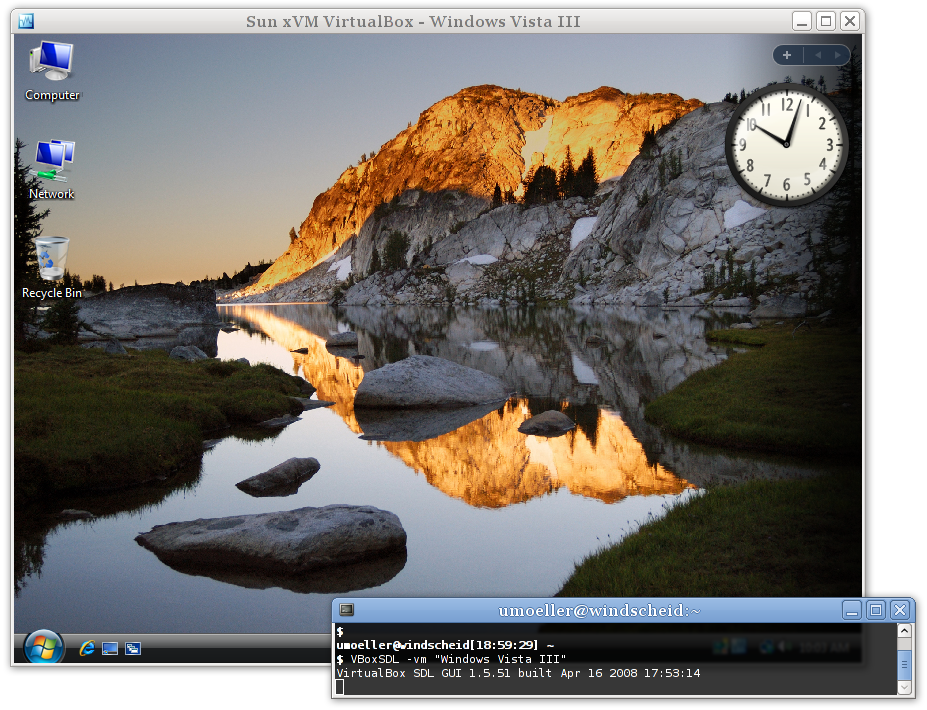
\includegraphics[width=10cm]{images/vbox-sdl.png}
\end{center}

To start a virtual machine with VBoxSDL instead of the VirtualBox
      GUI, enter the following on a command line:

\begin{Verbatim}[fontsize=\footnotesize]
VBoxSDL --startvm <vm>
\end{Verbatim}


where \texttt{<vm>} is, as usual
      with VirtualBox command line parameters, the name or UUID of an existing
      virtual machine.

\subsection{Secure labeling with VBoxSDL}


When running guest operating systems in full screen mode, the guest
      operating system usually has control over the whole screen. This could
      present a security risk as the guest operating system might fool the
      user into thinking that it is either a different system (which might
      have a higher security level) or it might present messages on the screen
      that appear to stem from the host operating system.

In order to protect the user against the above mentioned security
      risks, the secure labeling feature has been developed. Secure labeling
      is currently available only for VBoxSDL. When enabled, a portion of the
      display area is reserved for a label in which a user defined message is
      displayed. The label height in set to 20 pixels in VBoxSDL. The label
      font color and background color can be optionally set as hexadecimal RGB
      color values. The following syntax is used to enable secure
      labeling:

\begin{Verbatim}[fontsize=\footnotesize]
VBoxSDL --startvm "VM name"
      --securelabel --seclabelfnt ~/fonts/arial.ttf
      --seclabelsiz 14 --seclabelfgcol 00FF00 --seclabelbgcol 00FFFF
\end{Verbatim}


In addition to enabling secure labeling, a TrueType font has to be
      supplied. To use another font size than 12 point use the parameter
      \texttt{-{}-seclabelsiz}.

The label text can be set with 

\begin{Verbatim}[fontsize=\footnotesize]
VBoxManage setextradata "VM name" "VBoxSDL/SecureLabel" "The Label"
\end{Verbatim}

      Changing this label will take effect immediately.

Typically, full screen resolutions are limited to certain
      \OQ{}standard\CQ{} geometries such as 1024 x 768. Increasing this by twenty
      lines is not usually feasible, so in most cases, VBoxSDL will chose the
      next higher resolution, e.g. 1280 x 1024 and the guest's screen will not
      cover the whole display surface. If VBoxSDL is unable to choose a higher
      resolution, the secure label will be painted on top of the guest's
      screen surface. In order to address the problem of the bottom part of
      the guest screen being hidden, VBoxSDL can provide custom video modes to
      the guest that are reduced by the height of the label. For Windows
      guests and recent Solaris and Linux guests, the VirtualBox Guest
      Additions automatically provide the reduced video modes. Additionally,
      the VESA BIOS has been adjusted to duplicate its standard mode table
      with adjusted resolutions. The adjusted mode IDs can be calculated using
      the following formula:

\begin{Verbatim}[fontsize=\footnotesize]
reduced_modeid = modeid + 0x30
\end{Verbatim}


For example, in order to start Linux with 1024 x 748 x 16, the
      standard mode 0x117 (1024 x 768 x 16) is used as a base. The Linux video
      mode kernel parameter can then be calculated using:

\begin{Verbatim}[fontsize=\footnotesize]
vga = 0x200 | 0x117 + 0x30
vga = 839
\end{Verbatim}


The reason for duplicating the standard modes instead of only
      supplying the adjusted modes is that most guest operating systems
      require the standard VESA modes to be fixed and refuse to start with
      different modes.

When using the X.org VESA driver, custom modelines have to be
      calculated and added to the configuration (usually in
      /etc/X11/xorg.conf. A handy tool to determine
      modeline entries can be found at \url{http://www.tkk.fi/Misc/Electronics/faq/vga2rgb/calc.html}.)

\subsection{Releasing modifiers with VBoxSDL on Linux}


When switching from a X virtual terminal (VT) to another VT using
      Ctrl-Alt-Fx while the VBoxSDL window has the input focus, the guest will
      receive Ctrl and Alt keypress events without receiving the corresponding
      key release events. This is an architectural limitation of Linux. In
      order to reset the modifier keys, it is possible to send
      \texttt{SIGUSR1} to the VBoxSDL main thread
      (first entry in the \texttt{ps} list). For
      example, when switching away to another VT and saving the virtual
      machine from this terminal, the following sequence can be used to make
      sure the VM is not saved with stuck modifiers:



\begin{Verbatim}[fontsize=\footnotesize]
kill -usr1 <pid>
VBoxManage controlvm "Windows 2000" savestate
\end{Verbatim}


\section{Automated guest logons}
\label{autologon}


VirtualBox provides Guest Addition modules for Windows, Linux and
    Solaris to enable automated logons on the guest.

When a guest operating system is running in a virtual machine, it
    might be desirable to perform coordinated and automated logons using
    credentials from a master logon system. (With \OQ{}credentials\CQ{}, we are
    referring to logon information consisting of user name, password and
    domain name, where each value might be empty.)

\subsection{Automated Windows guest logons}
\label{autologon_win}


Since Windows NT, Windows has provided a modular system logon
      subsystem (\OQ{}Winlogon\CQ{}) which can be customized and extended by means of
      so-called GINA modules (Graphical Identification and Authentication).
      With Windows Vista and Windows 7, the GINA modules were replaced with a
      new mechanism called \OQ{}credential providers\CQ{}. The VirtualBox Guest
      Additions for Windows come with both, a GINA and a credential provider
      module, and therefore enable any Windows guest to perform automated
      logons.

To activate the VirtualBox GINA or credential provider module,
      install the Guest Additions with using the command line switch
      \texttt{/with\_autologon}. All the following
      manual steps required for installing these modules will be then done by
      the installer.

To manually install the VirtualBox GINA module, extract the Guest
      Additions (see chapter \ref{windows-guest-file-extraction}, \textit{\nameref{windows-guest-file-extraction}}, page \pageref{windows-guest-file-extraction}) and
      copy the file \texttt{VBoxGINA.dll} to the
      Windows \texttt{SYSTEM32} directory. Then, in
      the registry, create the following key: 

\begin{Verbatim}[fontsize=\footnotesize]
HKEY_LOCAL_MACHINE\SOFTWARE\Microsoft\Windows NT\CurrentVersion\Winlogon\GinaDLL
\end{Verbatim}

      with a value of \texttt{VBoxGINA.dll}.

\vspace{.2cm}

\begin{center}\fbox{\begin{minipage}[c]{0.9\textwidth}\color{colNote}\textbf{Note:} The VirtualBox GINA module is implemented as a wrapper around
        the standard Windows GINA module
        (\texttt{MSGINA.DLL}). As a result, it will
        most likely not work correctly with 3rd party GINA modules.\end{minipage}}\end{center}

\vspace{.2cm}



To manually install the VirtualBox credential provider module,
      extract the Guest Additions (see chapter \ref{windows-guest-file-extraction}, \textit{\nameref{windows-guest-file-extraction}}, page \pageref{windows-guest-file-extraction}) and copy the file
      \texttt{VBoxCredProv.dll} to the Windows
      \texttt{SYSTEM32} directory. Then, in the
      registry, create the following keys:

\begin{Verbatim}[fontsize=\footnotesize]
HKEY_LOCAL_MACHINE\SOFTWARE\Microsoft\Windows\CurrentVersion\
           Authentication\Credential Providers\{275D3BCC-22BB-4948-A7F6-3A3054EBA92B}

HKEY_CLASSES_ROOT\CLSID\{275D3BCC-22BB-4948-A7F6-3A3054EBA92B}

HKEY_CLASSES_ROOT\CLSID\{275D3BCC-22BB-4948-A7F6-3A3054EBA92B}\InprocServer32
\end{Verbatim}


with all default values (the key named
      \texttt{(Default)} in each key) set to
      \texttt{VBoxCredProv}. After that a new string
      named 

\begin{Verbatim}[fontsize=\footnotesize]
HKEY_CLASSES_ROOT\CLSID\{275D3BCC-22BB-4948-A7F6-3A3054EBA92B}\InprocServer32\ThreadingModel
\end{Verbatim}

      with a value of \texttt{Apartment} has to be
      created.

To set credentials, use the following command on a
      \textit{running} VM:

\begin{Verbatim}[fontsize=\footnotesize]
VBoxManage controlvm "Windows XP" setcredentials "John Doe" "secretpassword" "DOMTEST"
\end{Verbatim}


While the VM is running, the credentials can be queried by the
      VirtualBox logon modules (GINA or credential provider) using the
      VirtualBox Guest Additions device driver. When Windows is in \OQ{}logged
      out\CQ{} mode, the logon modules will constantly poll for credentials and if
      they are present, a logon will be attempted. After retrieving the
      credentials, the logon modules will erase them so that the above command
      will have to be repeated for subsequent logons.

For security reasons, credentials are not stored in any persistent
      manner and will be lost when the VM is reset. Also, the credentials are
      \OQ{}write-only\CQ{}, i.e. there is no way to retrieve the credentials from the
      host side. Credentials can be reset from the host side by setting empty
      values.

Depending on the particular variant of the Windows guest, the
      following restrictions apply: 

\begin{enumerate}


\item 

For \textbf{Windows XP guests,} the
            logon subsystem needs to be configured to use the classic logon
            dialog as the VirtualBox GINA module does not support the XP-style
            welcome dialog.


\item 

For \textbf{Windows Vista, Windows 7
            and Windows 8 guests,} the logon subsystem does not support
            the so-called Secure Attention Sequence
            (\texttt{CTRL+ALT+DEL}). As a result, the
            guest's group policy settings need to be changed to not use the
            Secure Attention Sequence. Also, the user name given is only
            compared to the true user name, not the user friendly name. This
            means that when you rename a user, you still have to supply the
            original user name (internally, Windows never renames user
            accounts).


\item 

Auto-logon handling of the built-in Windows Remote Desktop
            Service (formerly known as Terminal Services) is disabled by
            default. To enable it, create the registry key 

\begin{Verbatim}[fontsize=\footnotesize]
HKEY_LOCAL_MACHINE\SOFTWARE\Oracle\VirtualBox Guest Additions\AutoLogon
\end{Verbatim}

            with a \texttt{DWORD} value of
            \texttt{1}.

\end{enumerate}


The following command forces VirtualBox to keep the credentials
      after they were read by the guest and on VM reset: 

\begin{Verbatim}[fontsize=\footnotesize]
VBoxManage setextradata "Windows XP" VBoxInternal/Devices/VMMDev/0/Config/KeepCredentials 1
\end{Verbatim}
Note
      that this is a potential security risk as a malicious application
      running on the guest could request this information using the proper
      interface.

\subsection{Automated Linux/Unix guest logons}
\label{autologon_unix}


Starting with version 3.2, VirtualBox provides a custom PAM module
      (Pluggable Authentication Module) which can be used to perform automated
      guest logons on platforms which support this framework. Virtually all
      modern Linux/Unix distributions rely on PAM.

For automated logons on Ubuntu (or Ubuntu-derived) distributions
      using LightDM as the display manager, please see
      chapter \ref{autologon_unix_lightdm}, \textit{\nameref{autologon_unix_lightdm}}, page \pageref{autologon_unix_lightdm}.

The \texttt{pam\_vbox.so} module itself
      \textbf{does not} do an actual verification of
      the credentials passed to the guest OS; instead it relies on other
      modules such as \texttt{pam\_unix.so} or
      \texttt{pam\_unix2.so} down in the PAM stack to
      do the actual validation using the credentials retrieved by
      \texttt{pam\_vbox.so}. Therefore
      \texttt{pam\_vbox.so} has to be on top of the
      authentication PAM service list.

\vspace{.2cm}

\begin{center}\fbox{\begin{minipage}[c]{0.9\textwidth}\color{colNote}\textbf{Note:} The \texttt{pam\_vbox.so} only supports
        the \texttt{auth} primitive. Other primitives
        such as \texttt{account},
        \texttt{session} or
        \texttt{password} are not supported.\end{minipage}}\end{center}

\vspace{.2cm}



The \texttt{pam\_vbox.so} module is shipped
      as part of the Guest Additions but it is not installed and/or activated
      on the guest OS by default. In order to install it, it has to be copied
      from
      \texttt{/opt/VBoxGuestAdditions-<version>/lib/VBoxGuestAdditions/}
      to the security modules directory, usually
      \texttt{/lib/security/} on 32-bit guest Linuxes
      or \texttt{/lib64/security/} on 64-bit ones.
      Please refer to your guest OS documentation for the correct PAM module
      directory.

For example, to use \texttt{pam\_vbox.so}
      with a Ubuntu Linux guest OS and GDM (the GNOME Desktop Manager) to
      logon users automatically with the credentials passed by the host, the
      guest OS has to be configured like the following:

\begin{enumerate}


\item 

The \texttt{pam\_vbox.so} module has to
          be copied to the security modules directory, in this case it is
          \texttt{/lib/security}.


\item 

Edit the PAM configuration file for GDM found at
          \texttt{/etc/pam.d/gdm}, adding the line
          \texttt{auth requisite pam\_vbox.so} at the
          top. Additionaly, in most Linux distributions there is a file called
          \texttt{/etc/pam.d/common-auth}. This file
          is included in many other services (like the GDM file mentioned
          above). There you also have to add the line \texttt{auth
          requisite pam\_vbox.so}.


\item 

If authentication against the shadow database using
          \texttt{pam\_unix.so} or
          \texttt{pam\_unix2.so} is desired, the
          argument \texttt{try\_first\_pass} for
          \texttt{pam\_unix.so} or
          \texttt{use\_first\_pass} for
          \texttt{pam\_unix2.so} is needed in order to
          pass the credentials from the VirtualBox module to the shadow
          database authentication module. For Ubuntu, this needs to be added
          to \texttt{/etc/pam.d/common-auth}, to the
          end of the line referencing
          \texttt{pam\_unix.so}. This argument tells
          the PAM module to use credentials already present in the stack, i.e.
          the ones provided by the VirtualBox PAM module.

\end{enumerate}




\vspace{.2cm}

\begin{center}\fbox{\begin{minipage}[c]{0.9\textwidth}\color{colWarning}\textbf{Warning:} An incorrectly configured PAM stack can effectively prevent
          you from logging into your guest system!\end{minipage}}\end{center}

\vspace{.2cm}



To make deployment easier, you can pass the argument
      \texttt{debug} right after the
      \texttt{pam\_vbox.so} statement. Debug log output
      will then be recorded using syslog.



\vspace{.2cm}

\begin{center}\fbox{\begin{minipage}[c]{0.9\textwidth}\color{colNote}\textbf{Note:} By default, pam\_vbox will not wait for credentials to arrive
          from the host, in other words: When a login prompt is shown (for
          example by GDM/KDM or the text console) and pam\_vbox does not yet
          have credentials it does not wait until they arrive. Instead the
          next module in the PAM stack (depending on the PAM configuration)
          will have the chance for authentication.\end{minipage}}\end{center}

\vspace{.2cm}



Starting with VirtualBox 4.1.4 pam\_vbox supports various guest
      property parameters which all reside in
      \texttt{/VirtualBox/GuestAdd/PAM/}. These
      parameters allow pam\_vbox to wait for credentials to be provided by the
      host and optionally can show a message while waiting for those. The
      following guest properties can be set:

\begin{enumerate}


\item 

\texttt{CredsWait}: Set to \OQ{}1\CQ{} if
          pam\_vbox should start waiting until credentials arrive from the
          host. Until then no other authentication methods such as manually
          logging in will be available. If this property is empty or get
          deleted no waiting for credentials will be performed and pam\_vbox
          will act like before (see paragraph above). This property must be
          set read-only for the guest
          (\texttt{RDONLYGUEST}).


\item 

\texttt{CredsWaitAbort}: Aborts waiting
          for credentials when set to any value. Can be set from host and the
          guest.


\item 

\texttt{CredsWaitTimeout}: Timeout (in
          seconds) to let pam\_vbox wait for credentials to arrive. When no
          credentials arrive within this timeout, authentication of pam\_vbox
          will be set to failed and the next PAM module in chain will be
          asked. If this property is not specified, set to \OQ{}0\CQ{} or an invalid
          value, an infinite timeout will be used. This property must be set
          read-only for the guest
          (\texttt{RDONLYGUEST}).

\end{enumerate}


To customize pam\_vbox further there are the following guest
      properties:

\begin{enumerate}


\item 

\texttt{CredsMsgWaiting}: Custom
          message showed while pam\_vbox is waiting for credentials from the
          host. This property must be set read-only for the guest
          (\texttt{RDONLYGUEST}).


\item 

\texttt{CredsMsgWaitTimeout}: Custom
          message showed when waiting for credentials by pam\_vbox timed out,
          e.g. did not arrive within time. This property must be set read-only
          for the guest (\texttt{RDONLYGUEST}).

\end{enumerate}




\vspace{.2cm}

\begin{center}\fbox{\begin{minipage}[c]{0.9\textwidth}\color{colNote}\textbf{Note:} If a pam\_vbox guest property does not have set the right flags
          (\texttt{RDONLYGUEST}) this property will be
          ignored then and - depending on the property - a default value will
          be set. This can result in pam\_vbox not waiting for credentials.
          Consult the appropriate syslog file for more information and use the
          \texttt{debug} option.\end{minipage}}\end{center}

\vspace{.2cm}



\subsubsection{VirtualBox Greeter for Ubuntu / LightDM}
\label{autologon_unix_lightdm}


Starting with version 4.2.12, VirtualBox comes with an own greeter
        module named vbox-greeter which can be used with LightDM 1.0.1 or later.
        LightDM is the default display manager since Ubuntu 10.11 and therefore
        also can be used for automated guest logons.

vbox-greeter does not need the pam\_vbox module described above
        in order to function -- it comes with its own authentication mechanism
        provided by LightDM. However, to provide maximum of flexibility both
        modules can be used together on the same guest.

As for the pam\_vbox module, vbox-greeter is shipped as part of
        the Guest Additions but it is not installed and/or activated on the
        guest OS by default For installing vbox-greeter automatically upon
        Guest Additions installation, use the
        \texttt{-{}-with-autologon} switch when starting
        the VBoxLinuxAdditions.run file:

\begin{Verbatim}[fontsize=\footnotesize]
# ./VBoxLinuxAdditions.run -- --with-autologon
\end{Verbatim}


For manual or postponed installation, the
        \texttt{vbox-greeter.desktop}
        file has to be copied from
        \texttt{/opt/VBoxGuestAdditions-<version>/shared/VBoxGuestAdditions/}
        to the \texttt{xgreeters} directory, usually
        \texttt{/usr/share/xgreeters/}.
        Please refer to your guest OS documentation for the correct LightDM
        greeter directory.

The vbox-greeter module itself already was installed by the
        VirtualBox Guest Additions installer and resides in
        \texttt{/usr/sbin/}. To enable vbox-greeter as
        the standard greeter module, the file
        \texttt{/etc/lightdm/lightdm.conf} needs to be
        edited:



\begin{Verbatim}[fontsize=\footnotesize]
[SeatDefaults]
greeter-session=vbox-greeter
\end{Verbatim}


\vspace{.2cm}

\begin{center}\fbox{\begin{minipage}[c]{0.9\textwidth}\color{colNote}\textbf{Note:} The LightDM server needs to be fully restarted in order to
        get vbox-greeter used as the default greeter. As root, do a
        \texttt{service lightdm -{}-full-restart} on
        Ubuntu, or simply restart the guest.\end{minipage}}\end{center}

\vspace{.2cm}



\vspace{.2cm}

\begin{center}\fbox{\begin{minipage}[c]{0.9\textwidth}\color{colNote}\textbf{Note:} vbox-greeter is independent of the graphical session chosen
        by the user (like Gnome, KDE, Unity etc). However, it requires FLTK 1.3
        for representing its own user interface.\end{minipage}}\end{center}

\vspace{.2cm}



There are numerous guest properties which can be used to further
        customize the login experience. For automatically logging in users, the
        same guest properties apply as for pam\_vbox, see
        chapter \ref{autologon_unix}, \textit{\nameref{autologon_unix}}, page \pageref{autologon_unix}.

In addition to the above mentioned guest properties, vbox-greeter
        allows further customization of its user interface. These special guest
        properties all reside in
        \texttt{/VirtualBox/GuestAdd/Greeter/}:

\begin{enumerate}


\item 

\texttt{HideRestart}: Set to \OQ{}1\CQ{} if
            vbox-greeter should hide the button to restart the guest. This
            property must be set read-only for the guest
            (\texttt{RDONLYGUEST}).


\item 

\texttt{HideShutdown}: Set to \OQ{}1\CQ{} if
            vbox-greeter should hide the button to shutdown the guest. This
            property must be set read-only for the guest
            (\texttt{RDONLYGUEST}).


\item 

\texttt{BannerPath}: Path to a .PNG
            file for using it as a banner on the top. The image size must be
            460 x 90 pixels, any bit depth. This property must be
            set read-only for the guest
            (\texttt{RDONLYGUEST}).


\item 

\texttt{UseTheming}: Set to \OQ{}1\CQ{} for
            turning on the following theming options. This property must be
            set read-only for the guest
            (\texttt{RDONLYGUEST}).


\item 

\texttt{Theme/BackgroundColor}:
            Hexadecimal RRGGBB color for the background. This property must be
            set read-only for the guest
            (\texttt{RDONLYGUEST}).


\item 

\texttt{Theme/LogonDialog/HeaderColor}:
            Hexadecimal RRGGBB foreground color for the header text. This
            property must be set read-only for the guest
            (\texttt{RDONLYGUEST}).


\item 

\texttt{Theme/LogonDialog/BackgroundColor}:
            Hexadecimal RRGGBB color for the logon dialog background. This
            property must be set read-only for the guest
            (\texttt{RDONLYGUEST}).


\item 

\texttt{Theme/LogonDialog/ButtonColor}:
            Hexadecimal RRGGBB background color for the logon dialog button. This
            property must be set read-only for the guest
            (\texttt{RDONLYGUEST}).

\end{enumerate}


\vspace{.2cm}

\begin{center}\fbox{\begin{minipage}[c]{0.9\textwidth}\color{colNote}\textbf{Note:} The same restrictions for the guest properties above apply
        as for the ones specified in the pam\_vbox section.\end{minipage}}\end{center}

\vspace{.2cm}



\section{Advanced configuration for Windows guests}


\subsection{Automated Windows system preparation}
\label{sysprep}


Beginning with Windows NT 4.0, Microsoft offers a \OQ{}system
      preparation\CQ{} tool (in short: Sysprep) to prepare a Windows system for
      deployment or redistribution. Whereas Windows 2000 and XP ship with
      Sysprep on the installation medium, the tool also is available for
      download on the Microsoft web site. In a standard installation of
      Windows Vista and 7, Sysprep is already included. Sysprep mainly
      consists of an executable called
      \texttt{sysprep.exe} which is invoked by the
      user to put the Windows installation into preparation mode.

Starting with VirtualBox 3.2.2, the Guest Additions offer a way to
      launch a system preparation on the guest operating system in an
      automated way, controlled from the host system. To achieve that, see
      chapter \ref{guestadd-guestcontrol}, \textit{\nameref{guestadd-guestcontrol}}, page \pageref{guestadd-guestcontrol} for using the feature with the
      special identifier \texttt{sysprep} as the
      program to execute, along with the user name
      \texttt{sysprep} and password
      \texttt{sysprep} for the credentials. Sysprep
      then gets launched with the required system rights.

\vspace{.2cm}

\begin{center}\fbox{\begin{minipage}[c]{0.9\textwidth}\color{colNote}\textbf{Note:} Specifying the location of \OQ{}sysprep.exe\CQ{} is \textbf{not possible} -- instead the following paths are
        used (based on the operating system): 

\begin{itemize}


\item 

\texttt{C:\textbackslash{}sysprep\textbackslash{}sysprep.exe}
              for Windows NT 4.0, 2000 and XP


\item 

\texttt{\%WINDIR\%\textbackslash{}System32\textbackslash{}Sysprep\textbackslash{}sysprep.exe}
              for Windows Vista, 2008 Server and 7

\end{itemize}
 The Guest Additions will automatically use the
        appropriate path to execute the system preparation tool.\end{minipage}}\end{center}

\vspace{.2cm}



\section{Advanced configuration for Linux and Solaris guests}


\subsection{Manual setup of selected guest services on Linux}


The VirtualBox Guest Additions contain several different drivers.
      If for any reason you do not wish to set them all up, you can install
      the Guest Additions using the following command:

\begin{Verbatim}[fontsize=\footnotesize]
  sh ./VBoxLinuxAdditions.run no_setup
\end{Verbatim}


After this, you will need to at least compile the kernel modules
      by running the command 

\begin{Verbatim}[fontsize=\footnotesize]
  /usr/lib/VBoxGuestAdditions/vboxadd setup
\end{Verbatim}

      as root (you will need to replace \textit{lib} by
      \textit{lib64} on some 64bit guests), and on older guests
      without the udev service you will need to add the
      \textit{vboxadd} service to the default runlevel to ensure
      that the modules get loaded.

To setup the time synchronization service, run the command
      

\begin{Verbatim}[fontsize=\footnotesize]
  /usr/lib/VBoxGuestAdditions/vboxadd-service setup
\end{Verbatim}
 and
      add the service vboxadd-service to the default runlevel. To set up the
      X11 and OpenGL part of the Guest Additions, run the command 

\begin{Verbatim}[fontsize=\footnotesize]
  /usr/lib/VBoxGuestAdditions/vboxadd-x11 setup
\end{Verbatim}

      (you do not need to enable any services for this).

To recompile the guest kernel modules, use this command: 

\begin{Verbatim}[fontsize=\footnotesize]
  /usr/lib/VBoxGuestAdditions/vboxadd setup
\end{Verbatim}

      After compilation you should reboot your guest to ensure that the new
      modules are actually used.

\subsection{Guest graphics and mouse driver setup in depth}
\label{guestxorgsetup}


This section assumes that you are familiar with configuring the
      X.Org server using xorg.conf and optionally the newer mechanisms using
      hal or udev and xorg.conf.d. If not you can learn about them by studying
      the documentation which comes with X.Org.

The VirtualBox Guest Additions come with drivers for X.Org
      versions 

\begin{itemize}


\item 
            X11R6.8/X11R6.9 and XFree86 version 4.3 (vboxvideo\_drv\_68.o and vboxmouse\_drv\_68.o)
          


\item 
            X11R7.0 (vboxvideo\_drv\_70.so and vboxmouse\_drv\_70.so)
          


\item 
            X11R7.1 (vboxvideo\_drv\_71.so and vboxmouse\_drv\_71.so)
          


\item 
            X.Org Server versions 1.3 and later (vboxvideo\_drv\_13.so and vboxmouse\_drv\_13.so and so on).
          

\end{itemize}
 By default these drivers can be found in the
      directory

\texttt{/opt/VBoxGuestAdditions-<version>/lib/VBoxGuestAdditions}

and the correct versions for the X server are symbolically linked
      into the X.Org driver directories.

For graphics integration to work correctly, the X server must load
      the vboxvideo driver (many recent X server versions look for it
      automatically if they see that they are running in VirtualBox) and for
      an optimal user experience the guest kernel drivers must be loaded and
      the Guest Additions tool VBoxClient must be running as a client in the X
      session. For mouse integration to work correctly, the guest kernel
      drivers must be loaded and in addition, in X servers from X.Org X11R6.8
      to X11R7.1 and in XFree86 version 4.3 the right vboxmouse driver must be
      loaded and associated with /dev/mouse or /dev/psaux; in X.Org server 1.3
      or later a driver for a PS/2 mouse must be loaded and the right
      vboxmouse driver must be associated with /dev/vboxguest.

The VirtualBox guest graphics driver can use any graphics
      configuration for which the virtual resolution fits into the virtual
      video memory allocated to the virtual machine (minus a small amount used
      by the guest driver) as described in chapter \ref{settings-display}, \textit{\nameref{settings-display}}, page \pageref{settings-display}. The driver will offer a range of standard
      modes at least up to the default guest resolution for all active guest
      monitors. In X.Org Server 1.3 and later the default mode can be changed
      by setting the output property VBOX\_MODE to
      \OQ{}<width>x<height>\OQ{} for any guest monitor. When VBoxClient
      and the kernel drivers are active this is done automatically when the
      host requests a mode change. The driver for older versions can only
      receive new modes by querying the host for requests at regular
      intervals.

With pre-1.3 X Servers you can also add your own modes to the X
      server configuration file. You simply need to add them to the \OQ{}Modes\CQ{}
      list in the \OQ{}Display\CQ{} subsection of the \OQ{}Screen\CQ{} section. For example,
      the section shown here has a custom 2048x800 resolution mode
      added:

\begin{Verbatim}[fontsize=\footnotesize]
Section "Screen"
        Identifier    "Default Screen"
        Device        "VirtualBox graphics card"
        Monitor       "Generic Monitor"
        DefaultDepth  24
        SubSection "Display"
                Depth         24
                Modes         "2048x800" "800x600" "640x480"
        EndSubSection
EndSection
\end{Verbatim}


\section{CPU hot-plugging}
\label{cpuhotplug}


With virtual machines running modern server operating systems,
    VirtualBox supports CPU hot-plugging.\footnote{Support for CPU hot-plugging was introduced with VirtualBox
        3.2.} Whereas on a physical computer this would mean that a CPU
    can be added or removed while the machine is running, VirtualBox supports
    adding and removing virtual CPUs while a virtual machine is
    running.

CPU hot-plugging works only with guest operating systems that
    support it. So far this applies only to Linux and Windows Server 2008 x64
    Data Center Edition. Windows supports only hot-add while Linux supports
    hot-add and hot-remove but to use this feature with more than 8 CPUs a
    64bit Linux guest is required.

At this time, CPU hot-plugging requires using the VBoxManage
    command-line interface. First, hot-plugging needs to be enabled for a
    virtual machine:

\begin{Verbatim}[fontsize=\footnotesize]
VBoxManage modifyvm "VM name" --cpuhotplug on
\end{Verbatim}


After that, the --cpus option specifies the maximum number of CPUs
    that the virtual machine can have:

\begin{Verbatim}[fontsize=\footnotesize]
VBoxManage modifyvm "VM name" --cpus 8
\end{Verbatim}
When
    the VM is off, you can then add and remove virtual CPUs with the modifyvm
    --plugcpu and --unplugcpu subcommands, which take the number of the
    virtual CPU as a parameter, like this:

\begin{Verbatim}[fontsize=\footnotesize]
VBoxManage modifyvm "VM name" --plugcpu 3
VBoxManage modifyvm "VM name" --unplugcpu 3
\end{Verbatim}
Note that CPU 0 can never
    be removed.

While the VM is running, CPUs can be added with the
    \texttt{controlvm plugcpu/unplugcpu} commands
    instead:

\begin{Verbatim}[fontsize=\footnotesize]
VBoxManage controlvm "VM name" plugcpu 3
VBoxManage controlvm "VM name" unplugcpu 3
\end{Verbatim}


See chapter \ref{vboxmanage-modifyvm}, \textit{\nameref{vboxmanage-modifyvm}}, page \pageref{vboxmanage-modifyvm} and chapter \ref{vboxmanage-controlvm}, \textit{\nameref{vboxmanage-controlvm}}, page \pageref{vboxmanage-controlvm} for details.

With Linux guests, the following applies: To prevent ejection while
    the CPU is still used it has to be ejected from within the guest before.
    The Linux Guest Additions contain a service which receives hot-remove
    events and ejects the CPU. Also, after a CPU is added to the VM it is not
    automatically used by Linux. The Linux Guest Additions service will take
    care of that if installed. If not a CPU can be started with the following
    command:

\begin{Verbatim}[fontsize=\footnotesize]
echo 1 > /sys/devices/system/cpu/cpu<id>/online
\end{Verbatim}


\section{PCI passthrough}
\label{pcipassthrough}


When running on Linux hosts, with a recent enough kernel (at least
    version \texttt{2.6.31}) experimental host PCI
    devices passthrough is available.\footnote{Experimental support for PCI passthrough was introduced with
        VirtualBox 4.1.}

\vspace{.2cm}

\begin{center}\fbox{\begin{minipage}[c]{0.9\textwidth}\color{colNote}\textbf{Note:} The PCI passthrough module is shipped as a VirtualBox extension
      package, which must be installed separately. See chapter \ref{intro-installing}, \textit{\nameref{intro-installing}}, page \pageref{intro-installing} for more information.\end{minipage}}\end{center}

\vspace{.2cm}



Essentially this feature allows to directly use physical PCI devices
    on the host by the guest even if host doesn't have drivers for this
    particular device. Both, regular PCI and some PCI Express cards, are
    supported. AGP and certain PCI Express cards are not supported at the
    moment if they rely on GART (Graphics Address Remapping Table) unit
    programming for texture management as it does rather nontrivial operations
    with pages remapping interfering with IOMMU. This limitation may be lifted
    in future releases.

To be fully functional, PCI passthrough support in VirtualBox
    depends upon an IOMMU hardware unit which is not yet too widely available.
    If the device uses bus mastering (i.e. it performs DMA to the OS memory on
    its own), then an IOMMU is required, otherwise such DMA transactions may
    write to the wrong physical memory address as the device DMA engine is
    programmed using a device-specific protocol to perform memory
    transactions. The IOMMU functions as translation unit mapping physical
    memory access requests from the device using knowledge of the guest
    physical address to host physical addresses translation rules.

Intel's solution for IOMMU is marketed as \OQ{}Intel Virtualization
    Technology for Directed I/O\CQ{} (VT-d), and AMD's one is called AMD-Vi. So
    please check if your motherboard datasheet has appropriate technology.
    Even if your hardware doesn't have a IOMMU, certain PCI cards may work
    (such as serial PCI adapters), but the guest will show a warning on boot
    and the VM execution will terminate if the guest driver will attempt to
    enable card bus mastering.

It is very common that the BIOS or the host OS disables the IOMMU by
    default. So before any attempt to use it please make sure that
    

\begin{enumerate}


\item 

Your motherboard has an IOMMU unit.


\item 

Your CPU supports the IOMMU.


\item 

The IOMMU is enabled in the BIOS.


\item 

The VM must run with VT-x/AMD-V and nested paging
          enabled.


\item 

Your Linux kernel was compiled with IOMMU support (including
          DMA remapping, see \texttt{CONFIG\_DMAR}
          kernel compilation option). The PCI stub driver
          (\texttt{CONFIG\_PCI\_STUB}) is required as
          well.


\item 

Your Linux kernel recognizes and uses the IOMMU unit
          (\texttt{intel\_iommu=on} boot option could
          be needed). Search for DMAR and PCI-DMA in kernel boot log.

\end{enumerate}


Once you made sure that the host kernel supports the IOMMU, the next
    step is to select the PCI card and attach it to the guest. To figure out
    the list of available PCI devices, use the
    \texttt{lspci} command. The output will look like
    this:

\begin{Verbatim}[fontsize=\footnotesize]
01:00.0 VGA compatible controller: ATI Technologies Inc Cedar PRO [Radeon HD 5450]
01:00.1 Audio device: ATI Technologies Inc Manhattan HDMI Audio [Mobility Radeon HD 5000 Series]
02:00.0 Ethernet controller: Realtek Semiconductor Co., Ltd. RTL8111/8168B PCI Express Gigabit
        Ethernet controller (rev 03)
03:00.0 SATA controller: JMicron Technology Corp. JMB362/JMB363 Serial ATA Controller (rev 03)
03:00.1 IDE interface: JMicron Technology Corp. JMB362/JMB363 Serial ATA Controller (rev 03)
06:00.0 VGA compatible controller: nVidia Corporation G86 [GeForce 8500 GT] (rev a1)
\end{Verbatim}


The first column is a PCI address (in format
    \texttt{bus:device.function}). This address could
    be used to identify the device for further operations. For example, to
    attach a PCI network controller on the system listed above to the second
    PCI bus in the guest, as device 5, function 0, use the following command:
    

\begin{Verbatim}[fontsize=\footnotesize]
VBoxManage modifyvm "VM name" --pciattach 02:00.0@01:05.0
\end{Verbatim}

    To detach same device, use 

\begin{Verbatim}[fontsize=\footnotesize]
VBoxManage modifyvm "VM name" --pcidetach 02:00.0
\end{Verbatim}

    Please note that both host and guest could freely assign a different PCI
    address to the card attached during runtime, so those addresses only apply
    to the address of the card at the moment of attachment (host), and during
    BIOS PCI init (guest).

If the virtual machine has a PCI device attached, certain
    limitations apply: 

\begin{enumerate}


\item 
           Only PCI cards with non-shared interrupts (such as using MSI on host) are supported at the moment.
        


\item 
           No guest state can be reliably saved/restored (as the internal state of the PCI card could not be retrieved).
        


\item 
           Teleportation (live migration) doesn't work (for the same reason).
        


\item 
           No lazy physical memory allocation. The host will preallocate the whole RAM required for the VM on startup (as we cannot catch physical hardware accesses to the physical memory).
        

\end{enumerate}


\section{Webcam passthrough}


\subsection{Using a host webcam in the guest}
\label{webcam-passthrough}


VirtualBox 4.3 includes an experimental feature which allows a guest to use
      a host webcam. This complements the general USB passthrough support which was the
      typical way of using host webcams in earlier versions. The webcam passthrough support
      can handle non-USB video sources in theory, but this is completely untested.

\vspace{.2cm}

\begin{center}\fbox{\begin{minipage}[c]{0.9\textwidth}\color{colNote}\textbf{Note:} The webcam passthrough module is shipped as part of the Oracle VM VirtualBox
        extension pack, which must be installed separately. See chapter \ref{intro-installing}, \textit{\nameref{intro-installing}}, page \pageref{intro-installing} for more information.\end{minipage}}\end{center}

\vspace{.2cm}



The host webcam can be attached to the VM using \OQ{}Devices\CQ{} menu in the VM menu bar.
      The \OQ{}Webcams\CQ{} menu contains a list of available video input devices on the host.
      Clicking on a webcam name attaches or detaches the corresponding host device.

The VBoxManage command line tool can be used to enable webcam passthrough.
      Please see the host-specific sections below for additional details.
      The following commands are available:
        

\begin{itemize}


\item 

Get a list of host webcams (or other video input devices):
            

\begin{Verbatim}[fontsize=\footnotesize]
VBoxManage list webcams
\end{Verbatim}

            The output format:
            

\begin{Verbatim}[fontsize=\footnotesize]
alias "user friendly name"
host path or identifier
\end{Verbatim}

            The alias can be used as a shortcut in other commands. Alias '.0' means
            default video input device on the host, '.1', '.2', etc mean first, second, etc
            video input device. The device order is host-specific.
          


\item 

Attach a webcam to a running VM:
            

\begin{Verbatim}[fontsize=\footnotesize]
VBoxManage controlvm "VM name" webcam attach [host_path|alias [settings]]
\end{Verbatim}

            This will attach a USB webcam device to the guest.

The \texttt{settings} parameter is a string
            \texttt{Setting1=Value1;Setting2=Value2}, which allows to
            configure the emulated webcam device. The following settings are supported:
            

\begin{itemize}


\item \texttt{MaxFramerate} The highest rate at which video frames
                are sent to the guest. A higher frame rate requires more CPU power. Therefore sometimes
                it is useful to set a lower limit. Default is no limit and allow the guest to use all
                frame rates supported by the host webcam.
              


\item \texttt{MaxPayloadTransferSize} How many bytes the emulated
                webcam can send to the guest at a time. Default value is 3060 bytes, which is used by
                some webcams. Higher values can slightly reduce CPU load, if the guest is able to use
                larger buffers. However, a high \texttt{MaxPayloadTransferSize}
                might be not supported by some guests.
              

\end{itemize}

          


\item 

Detach a webcam from a running VM:
            

\begin{Verbatim}[fontsize=\footnotesize]
VBoxManage controlvm "VM name" webcam detach [host_path|alias]
\end{Verbatim}

          


\item 

List webcams attached to a running VM:
            

\begin{Verbatim}[fontsize=\footnotesize]
VBoxManage controlvm "VM name" webcam list
\end{Verbatim}

            The output contains path or alias which was used in 'webcam attach' command for
            each attached webcam.
          

\end{itemize}

      

\subsection{Windows hosts}


When the webcam device is detached from the host, the emulated webcam device is
      automatically detached from the guest.

\subsection{Mac OS X hosts}


OS X version 10.7 or newer is required.

When the webcam device is detached from the host, the emulated webcam device
      remains attached to the guest and must be manually detached using the
      \texttt{VBoxManage controlvm "VM name" webcam detach ...} command.

\subsection{Linux hosts}


When the webcam is detached from the host the emulated webcam device is
      automatically detached from the guest only if the webcam is streaming video.
      If the emulated webcam is inactive it should be manually detached using the
      \texttt{VBoxManage controlvm "VM name" webcam detach ...} command.

Aliases \texttt{.0} and \texttt{.1} are mapped
      to \texttt{/dev/video0}, alias \texttt{.2} is mapped
      to \texttt{/dev/video1} and so forth.

\section{Advanced display configuration}


\subsection{Custom VESA resolutions}


Apart from the standard VESA resolutions, the VirtualBox VESA BIOS
      allows you to add up to 16 custom video modes which will be reported to
      the guest operating system. When using Windows guests with the
      VirtualBox Guest Additions, a custom graphics driver will be used
      instead of the fallback VESA solution so this information does not
      apply.

Additional video modes can be configured for each VM using the
      extra data facility. The extra data key is called
      CustomVideoMode<x> with x
      being a number from 1 to 16. Please note that modes will be read from 1
      until either the following number is not defined or 16 is reached. The
      following example adds a video mode that corresponds to the native
      display resolution of many notebook computers:

\begin{Verbatim}[fontsize=\footnotesize]
VBoxManage setextradata "VM name" "CustomVideoMode1" "1400x1050x16"
\end{Verbatim}


The VESA mode IDs for custom video modes start at
      0x160. In order to use the above defined custom video
      mode, the following command line has be supplied to Linux:

\begin{Verbatim}[fontsize=\footnotesize]
vga = 0x200 | 0x160
vga = 864
\end{Verbatim}


For guest operating systems with VirtualBox Guest Additions, a
      custom video mode can be set using the video mode hint feature.

\subsection{Configuring the maximum resolution of guests when using the
      graphical frontend}


When guest systems with the Guest Additions installed are started
      using the graphical frontend (the normal VirtualBox application), they
      will not be allowed to use screen resolutions greater than the host's
      screen size unless the user manually resizes them by dragging the
      window, switching to full screen or seamless mode or sending a video mode
      hint using VBoxManage. This behavior is what most users will want, but
      if you have different needs, it is possible to change it by issuing one
      of the following commands from the command line:

\begin{Verbatim}[fontsize=\footnotesize]
VBoxManage setextradata global GUI/MaxGuestResolution any
\end{Verbatim}


will remove all limits on guest resolutions.

\begin{Verbatim}[fontsize=\footnotesize]
VBoxManage setextradata global GUI/MaxGuestResolution >width,height<
\end{Verbatim}


manually specifies a maximum resolution.

\begin{Verbatim}[fontsize=\footnotesize]
VBoxManage setextradata global GUI/MaxGuestResolution auto
\end{Verbatim}


restores the default settings. Note that these settings apply
      globally to all guest systems, not just to a single machine.

\section{Advanced storage configuration}


\subsection{Using a raw host hard disk from a guest}
\label{rawdisk}


Starting with version 1.4, as an alternative to using virtual disk
      images (as described in detail in chapter \ref{storage}, \textit{\nameref{storage}}, page \pageref{storage}),
      VirtualBox can also present either entire physical hard disks or
      selected partitions thereof as virtual disks to virtual machines.

With VirtualBox, this type of access is called \OQ{}raw hard disk
      access\CQ{}; it allows a guest operating system to access its virtual hard
      disk without going through the host OS file system. The actual
      performance difference for image files vs. raw disk varies greatly
      depending on the overhead of the host file system, whether dynamically
      growing images are used, and on host OS caching strategies. The caching
      indirectly also affects other aspects such as failure behavior, i.e.
      whether the virtual disk contains all data written before a host OS
      crash. Consult your host OS documentation for details on this.



\vspace{.2cm}

\begin{center}\fbox{\begin{minipage}[c]{0.9\textwidth}\color{colWarning}\textbf{Warning:} Raw hard disk access is for expert users only. Incorrect use
          or use of an outdated configuration can lead to \textbf{total loss of data }on the physical disk. Most
          importantly, \textit{do not} attempt to boot the
          partition with the currently running host operating system in a
          guest. This will lead to severe data corruption.\end{minipage}}\end{center}

\vspace{.2cm}



Raw hard disk access -- both for entire disks and individual
      partitions -- is implemented as part of the VMDK image format support.
      As a result, you will need to create a special VMDK image file which
      defines where the data will be stored. After creating such a special
      VMDK image, you can use it like a regular virtual disk image. For
      example, you can use the VirtualBox Manager (chapter \ref{vdis}, \textit{\nameref{vdis}}, page \pageref{vdis})
      or \texttt{VBoxManage} to assign the image to a
      virtual machine.

\subsubsection{Access to entire physical hard disk}


While this variant is the simplest to set up, you must be aware
        that this will give a guest operating system direct and full access to
        an \textit{entire physical disk}. If your
        \textit{host} operating system is also booted from this
        disk, please take special care to not access the partition from the
        guest at all. On the positive side, the physical disk can be
        repartitioned in arbitrary ways without having to recreate the image
        file that gives access to the raw disk.

To create an image that represents an entire physical hard disk
        (which will not contain any actual data, as this will all be stored on
        the physical disk), on a Linux host, use the command

\begin{Verbatim}[fontsize=\footnotesize]
VBoxManage internalcommands createrawvmdk -filename /path/to/file.vmdk
      -rawdisk /dev/sda
\end{Verbatim}
This creates the image
        \texttt{/path/to/file.vmdk} (must be absolute), and all data will
        be read and written from \texttt{/dev/sda}.

On a Windows host, instead of the above device specification,
        use e.g. \texttt{\textbackslash{}\textbackslash{}.\textbackslash{}PhysicalDrive0}. On a Mac OS X host, instead
        of the above device specification use e.g. \texttt{/dev/disk1}.
        Note that on OS X you can only get access to an entire disk if no
        volume is mounted from it.

Creating the image requires read/write access for the given
        device. Read/write access is also later needed when using the image
        from a virtual machine. On some host platforms (e.g. Windows Vista
        and later), raw disk access may be restricted and not permitted by
        the host OS in some situations.

Just like with regular disk images, this does not automatically
        attach the newly created image to a virtual machine. This can be done
        with e.g. 

\begin{Verbatim}[fontsize=\footnotesize]
VBoxManage storageattach WindowsXP --storagectl "IDE Controller"
      --port 0 --device 0 --type hdd --medium /path/to/file.vmdk
\end{Verbatim}
When
        this is done the selected virtual machine will boot from the specified
        physical disk.

\subsubsection{Access to individual physical hard disk partitions}


This \OQ{}raw partition support\CQ{} is quite similar to the \OQ{}full hard
        disk\CQ{} access described above. However, in this case, any partitioning
        information will be stored inside the VMDK image, so you can e.g.
        install a different boot loader in the virtual hard disk without
        affecting the host's partitioning information. While the guest will be
        able to \textit{see} all partitions that exist on the
        physical disk, access will be filtered in that reading from partitions
        for which no access is allowed the partitions will only yield zeroes,
        and all writes to them are ignored.

To create a special image for raw partition support (which will
        contain a small amount of data, as already mentioned), on a Linux
        host, use the command

\begin{Verbatim}[fontsize=\footnotesize]
VBoxManage internalcommands createrawvmdk -filename /path/to/file.vmdk
      -rawdisk /dev/sda -partitions 1,5
\end{Verbatim}


As you can see, the command is identical to the one for \OQ{}full
        hard disk\CQ{} access, except for the additional
        \texttt{-partitions} parameter. This example
        would create the image \texttt{/path/to/file.vmdk} (which, again,
        must be absolute), and partitions 1 and 5 of \texttt{/dev/sda}
        would be made accessible to the guest.

VirtualBox uses the same partition numbering as your Linux host.
        As a result, the numbers given in the above example would refer to the
        first primary partition and the first logical drive in the extended
        partition, respectively.

On a Windows host, instead of the above device specification,
        use e.g. \texttt{\textbackslash{}\textbackslash{}.\textbackslash{}PhysicalDrive0}. On a Mac OS X host, instead
        of the above device specification use e.g. \texttt{/dev/disk1}.
        Note that on OS X you can only use partitions which are not mounted
        (eject the respective volume first). Partition numbers are the same on
        Linux, Windows and Mac OS X hosts.

The numbers for the list of partitions can be taken from the
        output of

\begin{Verbatim}[fontsize=\footnotesize]
VBoxManage internalcommands listpartitions -rawdisk /dev/sda
\end{Verbatim}
The
        output lists the partition types and sizes to give the user enough
        information to identify the partitions necessary for the guest.

Images which give access to individual partitions are specific
        to a particular host disk setup. You cannot transfer these images to
        another host; also, whenever the host partitioning changes, the image
        \textit{must be recreated}.

Creating the image requires read/write access for the given
        device. Read/write access is also later needed when using the image
        from a virtual machine. If this is not feasible, there is a special
        variant for raw partition access (currently only available on Linux
        hosts) that avoids having to give the current user access to the
        entire disk. To set up such an image, use

\begin{Verbatim}[fontsize=\footnotesize]
VBoxManage internalcommands createrawvmdk -filename /path/to/file.vmdk
      -rawdisk /dev/sda -partitions 1,5 -relative
\end{Verbatim}
When used from a
        virtual machine, the image will then refer not to the entire disk, but
        only to the individual partitions (in the example
        \texttt{/dev/sda1} and \texttt{/dev/sda5}). As a consequence,
        read/write access is only required for the affected partitions, not
        for the entire disk. During creation however, read-only access to the
        entire disk is required to obtain the partitioning information.

In some configurations it may be necessary to change the MBR
        code of the created image, e.g. to replace the Linux boot loader that
        is used on the host by another boot loader. This allows e.g. the guest
        to boot directly to Windows, while the host boots Linux from the
        \OQ{}same\CQ{} disk. For this purpose the
        \texttt{-mbr} parameter is provided. It
        specifies a file name from which to take the MBR code. The partition
        table is not modified at all, so a MBR file from a system with totally
        different partitioning can be used. An example of this is

\begin{Verbatim}[fontsize=\footnotesize]
VBoxManage internalcommands createrawvmdk -filename /path/to/file.vmdk
      -rawdisk /dev/sda -partitions 1,5 -mbr winxp.mbr
\end{Verbatim}
The modified
        MBR will be stored inside the image, not on the host disk.

The created image can be attached to a storage controller in a
        VM configuration as usual.

\subsection{Configuring the hard disk vendor product data (VPD)}
\label{changevpd}


VirtualBox reports vendor product data for its virtual hard disks
      which consist of hard disk serial number, firmware revision and model
      number. These can be changed using the following commands:

\begin{Verbatim}[fontsize=\footnotesize]
VBoxManage setextradata "VM name"
      "VBoxInternal/Devices/ahci/0/Config/Port0/SerialNumber" "serial"
VBoxManage setextradata "VM name"
      "VBoxInternal/Devices/ahci/0/Config/Port0/FirmwareRevision" "firmware"
VBoxManage setextradata "VM name"
      "VBoxInternal/Devices/ahci/0/Config/Port0/ModelNumber" "model"
\end{Verbatim}


The serial number is a 20 byte alphanumeric string, the firmware
      revision an 8 byte alphanumeric string and the model number a 40 byte
      alphanumeric string. Instead of \OQ{}Port0\CQ{} (referring to the first port),
      specify the desired SATA hard disk port.

The above commands apply to virtual machines with an AHCI (SATA)
      controller. The commands for virtual machines with an IDE controller
      are:

\begin{Verbatim}[fontsize=\footnotesize]
VBoxManage setextradata "VM name"
      "VBoxInternal/Devices/piix3ide/0/Config/PrimaryMaster/SerialNumber" "serial"
VBoxManage setextradata "VM name"
      "VBoxInternal/Devices/piix3ide/0/Config/PrimaryMaster/FirmwareRevision" "firmware"
VBoxManage setextradata "VM name"
      "VBoxInternal/Devices/piix3ide/0/Config/PrimaryMaster/ModelNumber" "model"
\end{Verbatim}


For hard disks it's also possible to mark the
      drive as having a non-rotational medium with:

\begin{Verbatim}[fontsize=\footnotesize]
VBoxManage setextradata "VM name"
      "VBoxInternal/Devices/ahci/0/Config/Port0/NonRotational" "1"
\end{Verbatim}


Additional three parameters are needed for CD/DVD drives to report
      the vendor product data:

\begin{Verbatim}[fontsize=\footnotesize]
VBoxManage setextradata "VM name"
      "VBoxInternal/Devices/ahci/0/Config/Port0/ATAPIVendorId" "vendor"
VBoxManage setextradata "VM name"
      "VBoxInternal/Devices/ahci/0/Config/Port0/ATAPIProductId" "product"
VBoxManage setextradata "VM name"
      "VBoxInternal/Devices/ahci/0/Config/Port0/ATAPIRevision" "revision"
\end{Verbatim}


The vendor id is an 8 byte alphanumeric string, the product id an
      16 byte alphanumeric string and the revision a 4 byte alphanumeric
      string. Instead of \OQ{}Port0\CQ{} (referring to the first port), specify the
      desired SATA hard disk port.

\subsection{Access iSCSI targets via Internal Networking}
\label{iscsi-intnet}


As an experimental feature, VirtualBox allows for accessing an
      iSCSI target running in a virtual machine which is configured for using
      Internal Networking mode. Please see chapter \ref{storage-iscsi}, \textit{\nameref{storage-iscsi}}, page \pageref{storage-iscsi};
      chapter \ref{network_internal}, \textit{\nameref{network_internal}}, page \pageref{network_internal}; and chapter \ref{vboxmanage-storageattach}, \textit{\nameref{vboxmanage-storageattach}}, page \pageref{vboxmanage-storageattach} for additional information.

The IP stack accessing Internal Networking must be configured in
      the virtual machine which accesses the iSCSI target. A free static IP
      and a MAC address not used by other virtual machines must be chosen. In
      the example below, adapt the name of the virtual machine, the MAC
      address, the IP configuration and the Internal Networking name
      (\OQ{}MyIntNet\CQ{}) according to your needs. The following eight commands must
      first be issued:

\begin{Verbatim}[fontsize=\footnotesize]
VBoxManage setextradata "VM name" VBoxInternal/Devices/IntNetIP/0/Trusted 1
VBoxManage setextradata "VM name" VBoxInternal/Devices/IntNetIP/0/Config/MAC 08:00:27:01:02:0f
VBoxManage setextradata "VM name" VBoxInternal/Devices/IntNetIP/0/Config/IP 10.0.9.1
VBoxManage setextradata "VM name" VBoxInternal/Devices/IntNetIP/0/Config/Netmask 255.255.255.0
VBoxManage setextradata "VM name" VBoxInternal/Devices/IntNetIP/0/LUN#0/Driver IntNet
VBoxManage setextradata "VM name" VBoxInternal/Devices/IntNetIP/0/LUN#0/Config/Network MyIntNet
VBoxManage setextradata "VM name" VBoxInternal/Devices/IntNetIP/0/LUN#0/Config/TrunkType 2
VBoxManage setextradata "VM name" VBoxInternal/Devices/IntNetIP/0/LUN#0/Config/IsService 1
\end{Verbatim}


Finally the iSCSI disk must be attached with the
      \texttt{-{}-intnet} option to tell the iSCSI
      initiator to use internal networking:

\begin{Verbatim}[fontsize=\footnotesize]
VBoxManage storageattach ... --medium iscsi
         --server 10.0.9.30 --target iqn.2008-12.com.sun:sampletarget --intnet
\end{Verbatim}


Compared to a \OQ{}regular\CQ{} iSCSI setup, IP address of the target
      \textit{must} be specified as a numeric IP address, as there
      is no DNS resolver for internal networking.

The virtual machine with the iSCSI target should be started before
      the VM using it is powered on. If a virtual machine using an iSCSI disk
      is started without having the iSCSI target powered up, it can take up to
      200 seconds to detect this situation. The VM will fail to power
      up.

\section{Legacy commands for using serial ports}


Starting with version 1.4, VirtualBox provided support for virtual
    serial ports, which, at the time, was rather complicated to set up with a
    sequence of \texttt{VBoxManage setextradata}
    statements. Since version 1.5, that way of setting up serial ports is no
    longer necessary and \textit{deprecated.} To set up virtual
    serial ports, use the methods now described in chapter \ref{serialports}, \textit{\nameref{serialports}}, page \pageref{serialports}.

\vspace{.2cm}

\begin{center}\fbox{\begin{minipage}[c]{0.9\textwidth}\color{colNote}\textbf{Note:} For backwards compatibility, the old
        \texttt{setextradata} statements, whose
        description is retained below from the old version of the manual, take
        \textit{precedence} over the new way of configuring serial
        ports. As a result, if configuring serial ports the new way doesn't
        work, make sure the VM in question does not have old configuration
        data such as below still active.\end{minipage}}\end{center}

\vspace{.2cm}



The old sequence of configuring a serial port used the following 6
    commands:

\begin{Verbatim}[fontsize=\footnotesize]
VBoxManage setextradata "VM name"
      "VBoxInternal/Devices/serial/0/Config/IRQ" 4
VBoxManage setextradata "VM name"
      "VBoxInternal/Devices/serial/0/Config/IOBase" 0x3f8
VBoxManage setextradata "VM name"
      "VBoxInternal/Devices/serial/0/LUN#0/Driver" Char
VBoxManage setextradata "VM name"
      "VBoxInternal/Devices/serial/0/LUN#0/AttachedDriver/Driver" NamedPipe
VBoxManage setextradata "VM name"
      "VBoxInternal/Devices/serial/0/LUN#0/AttachedDriver/Config/Location" "\\.\pipe\vboxCOM1"
VBoxManage setextradata "VM name"
      "VBoxInternal/Devices/serial/0/LUN#0/AttachedDriver/Config/IsServer" 1
\end{Verbatim}


This sets up a serial port in the guest with the default settings
    for COM1 (IRQ 4, I/O address 0x3f8) and the
    \texttt{Location} setting assumes that this
    configuration is used on a Windows host, because the Windows named pipe
    syntax is used. Keep in mind that on Windows hosts a named pipe must
    always start with \texttt{\textbackslash{}\textbackslash{}.\textbackslash{}pipe\textbackslash{}}. On Linux the
    same configuration settings apply, except that the path name for the
    \texttt{Location} can be chosen more freely. Local
    domain sockets can be placed anywhere, provided the user running
    VirtualBox has the permission to create a new file in the directory. The
    final command above defines that VirtualBox acts as a server, i.e. it
    creates the named pipe itself instead of connecting to an already existing
    one.

\section{Fine-tuning the VirtualBox NAT engine}
\label{changenat}


\subsection{Configuring the address of a NAT network interface}


In NAT mode, the guest network interface is assigned to the IPv4
      range \texttt{10.0.x.0/24} by default where
      \texttt{x} corresponds to the instance of the
      NAT interface +2. So \texttt{x} is 2 when there
      is only one NAT instance active. In that case the guest is assigned to
      the address \texttt{10.0.2.15}, the gateway is
      set to \texttt{10.0.2.2} and the name server can
      be found at \texttt{10.0.2.3}.

If, for any reason, the NAT network needs to be changed, this can
      be achieved with the following command:

\begin{Verbatim}[fontsize=\footnotesize]
VBoxManage modifyvm "VM name" --natnet1 "192.168/16"
\end{Verbatim}


This command would reserve the network addresses from
      \texttt{192.168.0.0} to
      \texttt{192.168.254.254} for the first NAT
      network instance of \OQ{}VM name\CQ{}. The guest IP would be assigned to
      \texttt{192.168.0.15} and the default gateway
      could be found at \texttt{192.168.0.2}.

\subsection{Configuring the boot server (next server) of a NAT network
      interface}
\label{nat-adv-tftp}


For network booting in NAT mode, by default VirtualBox uses a
      built-in TFTP server at the IP address 10.0.2.4. This default behavior
      should work fine for typical remote-booting scenarios. However, it is
      possible to change the boot server IP and the location of the boot image
      with the following commands: 

\begin{Verbatim}[fontsize=\footnotesize]
VBoxManage modifyvm "VM name" --nattftpserver1 10.0.2.2
VBoxManage modifyvm "VM name" --nattftpfile1 /srv/tftp/boot/MyPXEBoot.pxe
\end{Verbatim}


\subsection{Tuning TCP/IP buffers for NAT}
\label{nat-adv-settings}


The VirtualBox NAT stack performance is often determined by its
      interaction with the host's TCP/IP stack and the size of several buffers
      (\texttt{SO\_RCVBUF} and
      \texttt{SO\_SNDBUF}). For certain setups users
      might want to adjust the buffer size for a better performance. This can
      by achieved using the following commands (values are in kilobytes and
      can range from 8 to 1024): 

\begin{Verbatim}[fontsize=\footnotesize]
VBoxManage modifyvm "VM name" --natsettings1 16000,128,128,0,0
\end{Verbatim}

      This example illustrates tuning the NAT settings. The first parameter is
      the MTU, then the size of the socket's send buffer and the size of the
      socket's receive buffer, the initial size of the TCP send window, and
      lastly the initial size of the TCP receive window. Note that specifying
      zero means fallback to the default value.

Each of these buffers has a default size of 64KB and default MTU
      is 1500.

\subsection{Binding NAT sockets to a specific interface}


By default, VirtualBox's NAT engine will route TCP/IP packets
      through the default interface assigned by the host's TCP/IP stack. (The
      technical reason for this is that the NAT engine uses sockets for
      communication.) If, for some reason, you want to change this behavior,
      you can tell the NAT engine to bind to a particular IP address instead.
      Use the following command: 

\begin{Verbatim}[fontsize=\footnotesize]
VBoxManage modifyvm "VM name" --natbindip1 "10.45.0.2"
\end{Verbatim}


After this, all outgoing traffic will be sent through the
      interface with the IP address 10.45.0.2. Please make sure that this
      interface is up and running prior to this assignment.

\subsection{Enabling DNS proxy in NAT mode}
\label{nat-adv-dns}


The NAT engine by default offers the same DNS servers to the guest
      that are configured on the host. In some scenarios, it can be desirable
      to hide the DNS server IPs from the guest, for example when this
      information can change on the host due to expiring DHCP leases. In this
      case, you can tell the NAT engine to act as DNS proxy using the
      following command: 

\begin{Verbatim}[fontsize=\footnotesize]
VBoxManage modifyvm "VM name" --natdnsproxy1 on
\end{Verbatim}


\subsection{Using the host's resolver as a DNS proxy in NAT mode}
\label{nat_host_resolver_proxy}


For resolving network names, the DHCP server of the NAT engine
      offers a list of registered DNS servers of the host. If for some reason
      you need to hide this DNS server list and use the host's resolver
      settings, thereby forcing the VirtualBox NAT engine to intercept DNS
      requests and forward them to host's resolver, use the following command:
      

\begin{Verbatim}[fontsize=\footnotesize]
VBoxManage modifyvm "VM name" --natdnshostresolver1 on
\end{Verbatim}

      Note that this setting is similar to the DNS proxy mode, however whereas
      the proxy mode just forwards DNS requests to the appropriate servers,
      the resolver mode will interpret the DNS requests and use the host's DNS
      API to query the information and return it to the guest.

\subsubsection{User-defined host name resolving}
\label{nat_host_resolver_name_intercepting}


In some cases it might be useful to intercept the name resolving mechanism,
            providing a user-defined IP address on a particular DNS request. The intercepting
            mechanism allows the user to map not only a single host but domains and even more
            complex namings conventions if required.


              The following command sets a rule for mapping a name to a specified IP:

\begin{Verbatim}[fontsize=\footnotesize]
VBoxManage setextradata "VM name" \
      "VBoxInternal/Devices/{pcnet,e1000}/0/LUN#0/Config/HostResolverMappings/ \
      <uniq name of interception rule>/HostIP" <IPv4>
VBoxManage setextradata "VM name" \
      "VBoxInternal/Devices/{pcnet,e1000}/0/LUN#0/Config/HostResolverMappings/ \
      <uniq name of interception rule>/HostName" <name of host>
\end{Verbatim}


The following command sets a rule for mapping a pattern name to a specified IP:

\begin{Verbatim}[fontsize=\footnotesize]
VBoxManage setextradata "VM name" \
      "VBoxInternal/Devices/{pcnet,e1000}/0/LUN#0/Config/HostResolverMappings/ \
      <uniq name of interception rule>/HostIP" <IPv4>
VBoxManage setextradata "VM name" \
      "VBoxInternal/Devices/{pcnet,e1000}/0/LUN#0/Config/HostResolverMappings/ \
      <uniq name of interception rule>/HostNamePattern" <hostpattern>
\end{Verbatim}


The host pattern may include \texttt{"|", "?" and "*"}.

This example demonstrates how to instruct the host-resolver mechanism to resolve
      all domain and probably some mirrors of www.blocked-site.info site with IP 127.0.0.1:

\begin{Verbatim}[fontsize=\footnotesize]
VBoxManage setextradata "VM name" \
      "VBoxInternal/Devices/e1000/0/LUN#0/Config/HostResolverMappings/ \
      all_blocked_site/HostIP" 127.0.0.1
VBoxManage setextradata "VM name" \
      "VBoxInternal/Devices/e1000/0/LUN#0/Config/HostResolverMappings/ \
      all_blocked_site/HostNamePattern" "*.blocked-site.*|*.fb.org"
\end{Verbatim}


\vspace{.2cm}

\begin{center}\fbox{\begin{minipage}[c]{0.9\textwidth}\color{colNote}\textbf{Note:} The host resolver mechanism should be enabled to use user-defined
             mapping rules (please see
             chapter \ref{nat_host_resolver_proxy}, \textit{\nameref{nat_host_resolver_proxy}}, page \pageref{nat_host_resolver_proxy} for more details).\end{minipage}}\end{center}

\vspace{.2cm}



\subsection{Configuring aliasing of the NAT engine}
\label{nat-adv-alias}


By default, the NAT core uses aliasing and uses random ports when
      generating an alias for a connection. This works well for the most
      protocols like SSH, FTP and so on. Though some protocols might need a
      more transparent behavior or may depend on the real port number the
      packet was sent from. It is possible to change the NAT mode via the
      VBoxManage frontend with the following commands: 

\begin{Verbatim}[fontsize=\footnotesize]
VBoxManage modifyvm "VM name" --nataliasmode1 proxyonly
\end{Verbatim}

      and 

\begin{Verbatim}[fontsize=\footnotesize]
VBoxManage modifyvm "Linux Guest" --nataliasmode1 sameports
\end{Verbatim}

      The first example disables aliasing and switches NAT into transparent
      mode, the second example enforces preserving of port values. These modes
      can be combined if necessary.

\section{Configuring the BIOS DMI information}
\label{changedmi}


The DMI data VirtualBox provides to guests can be changed for a
    specific VM. Use the following commands to configure the DMI BIOS
    information. In case your VM is configured to use EFI firmware you need to
    replace \texttt{pcbios} by \texttt{efi} in the keys.

\subsection{DMI BIOS information (type 0)}


\begin{Verbatim}[fontsize=\footnotesize]
VBoxManage setextradata "VM name"
      "VBoxInternal/Devices/pcbios/0/Config/DmiBIOSVendor"        "BIOS Vendor"
VBoxManage setextradata "VM name"
      "VBoxInternal/Devices/pcbios/0/Config/DmiBIOSVersion"       "BIOS Version"
VBoxManage setextradata "VM name"
      "VBoxInternal/Devices/pcbios/0/Config/DmiBIOSReleaseDate"   "BIOS Release Date"
VBoxManage setextradata "VM name"
      "VBoxInternal/Devices/pcbios/0/Config/DmiBIOSReleaseMajor"  1
VBoxManage setextradata "VM name"
      "VBoxInternal/Devices/pcbios/0/Config/DmiBIOSReleaseMinor"  2
VBoxManage setextradata "VM name"
      "VBoxInternal/Devices/pcbios/0/Config/DmiBIOSFirmwareMajor" 3
VBoxManage setextradata "VM name"
      "VBoxInternal/Devices/pcbios/0/Config/DmiBIOSFirmwareMinor" 4
\end{Verbatim}


\subsection{DMI system information (type 1)}


\begin{Verbatim}[fontsize=\footnotesize]
VBoxManage setextradata "VM name"
      "VBoxInternal/Devices/pcbios/0/Config/DmiSystemVendor"      "System Vendor"
VBoxManage setextradata "VM name"
      "VBoxInternal/Devices/pcbios/0/Config/DmiSystemProduct"     "System Product"
VBoxManage setextradata "VM name"
      "VBoxInternal/Devices/pcbios/0/Config/DmiSystemVersion"     "System Version"
VBoxManage setextradata "VM name"
      "VBoxInternal/Devices/pcbios/0/Config/DmiSystemSerial"      "System Serial"
VBoxManage setextradata "VM name"
      "VBoxInternal/Devices/pcbios/0/Config/DmiSystemSKU"         "System SKU"
VBoxManage setextradata "VM name"
      "VBoxInternal/Devices/pcbios/0/Config/DmiSystemFamily"      "System Family"
VBoxManage setextradata "VM name"
      "VBoxInternal/Devices/pcbios/0/Config/DmiSystemUuid"
                                               "9852bf98-b83c-49db-a8de-182c42c7226b"
\end{Verbatim}


\subsection{DMI board information (type 2)}


\begin{Verbatim}[fontsize=\footnotesize]
VBoxManage setextradata "VM name"
      "VBoxInternal/Devices/pcbios/0/Config/DmiBoardVendor"       "Board Vendor"
VBoxManage setextradata "VM name"
      "VBoxInternal/Devices/pcbios/0/Config/DmiBoardProduct"      "Board Product"
VBoxManage setextradata "VM name"
      "VBoxInternal/Devices/pcbios/0/Config/DmiBoardVersion"      "Board Version"
VBoxManage setextradata "VM name"
      "VBoxInternal/Devices/pcbios/0/Config/DmiBoardSerial"       "Board Serial"
VBoxManage setextradata "VM name"
      "VBoxInternal/Devices/pcbios/0/Config/DmiBoardAssetTag"     "Board Tag"
VBoxManage setextradata "VM name"
      "VBoxInternal/Devices/pcbios/0/Config/DmiBoardLocInChass"   "Board Location"
VBoxManage setextradata "VM name"
      "VBoxInternal/Devices/pcbios/0/Config/DmiBoardBoardType"    10
\end{Verbatim}


\subsection{DMI system enclosure or chassis (type 3)}


\begin{Verbatim}[fontsize=\footnotesize]
VBoxManage setextradata "VM name"
      "VBoxInternal/Devices/pcbios/0/Config/DmiChassisVendor"     "Chassis Vendor"
VBoxManage setextradata "VM name"
      "VBoxInternal/Devices/pcbios/0/Config/DmiChassisType"       3
VBoxManage setextradata "VM name"
      "VBoxInternal/Devices/pcbios/0/Config/DmiChassisVersion"    "Chassis Version"
VBoxManage setextradata "VM name"
      "VBoxInternal/Devices/pcbios/0/Config/DmiChassisSerial"     "Chassis Serial"
VBoxManage setextradata "VM name"
      "VBoxInternal/Devices/pcbios/0/Config/DmiChassisAssetTag"   "Chassis Tag"
\end{Verbatim}


\subsection{DMI processor informatiion (type 4)}


\begin{Verbatim}[fontsize=\footnotesize]
VBoxManage setextradata "VM name"
      "VBoxInternal/Devices/pcbios/0/Config/DmiProcManufacturer"  "GenuineIntel"
VBoxManage setextradata "VM name"
      "VBoxInternal/Devices/pcbios/0/Config/DmiProcVersion"       "Pentium(R) III"
\end{Verbatim}


\subsection{DMI OEM strings (type 11)}


\begin{Verbatim}[fontsize=\footnotesize]
VBoxManage setextradata "VM name"
      "VBoxInternal/Devices/pcbios/0/Config/DmiOEMVBoxVer"        "vboxVer_1.2.3"
VBoxManage setextradata "VM name"
      "VBoxInternal/Devices/pcbios/0/Config/DmiOEMVBoxRev"        "vboxRev_12345"
\end{Verbatim}


If a DMI string is not set, the default value of VirtualBox is used.
    To set an empty string use
    \texttt{"<EMPTY>"}.

Note that in the above list, all quoted parameters (DmiBIOSVendor,
    DmiBIOSVersion but not DmiBIOSReleaseMajor) are expected to be strings. If
    such a string is a valid number, the parameter is treated as number and
    the VM will most probably refuse to start with an
    \texttt{VERR\_CFGM\_NOT\_STRING} error. In that case,
    use \texttt{"string:<value>"}, for instance
    

\begin{Verbatim}[fontsize=\footnotesize]
VBoxManage setextradata "VM name"
      "VBoxInternal/Devices/pcbios/0/Config/DmiSystemSerial"      "string:1234"
\end{Verbatim}


Changing this information can be necessary to provide the DMI
    information of the host to the guest to prevent Windows from asking for a
    new product key. On Linux hosts the DMI BIOS information can be obtained
    with 

\begin{Verbatim}[fontsize=\footnotesize]
dmidecode -t0
\end{Verbatim}
and the DMI system information can be
    obtained with 

\begin{Verbatim}[fontsize=\footnotesize]
dmidecode -t1
\end{Verbatim}


\section{Configuring the custom ACPI table}
\label{changeacpicust}


VirtualBox can be configured to present an custom ACPI table to
    the guest. Use the following command to configure this:

\begin{Verbatim}[fontsize=\footnotesize]
VBoxManage setextradata "VM name"
      "VBoxInternal/Devices/acpi/0/Config/CustomTable" "/path/to/table.bin"
\end{Verbatim}


Configuring a custom ACPI table can prevent Windows
      Vista and Windows 7 from asking for a new product key. On Linux hosts,
      one of the host tables can be read from
    /sys/firmware/acpi/tables/.

\section{Fine-tuning timers and time synchronization}


\subsection{Configuring the guest time stamp counter (TSC) to reflect guest
      execution}
\label{changetscmode}


By default, VirtualBox keeps all sources of time visible to the
      guest synchronized to a single time source, the monotonic host time.
      This reflects the assumptions of many guest operating systems, which
      expect all time sources to reflect \OQ{}wall clock\CQ{} time. In special
      circumstances it may be useful however to make the TSC (time stamp
      counter) in the guest reflect the time actually spent executing the
      guest.

This special TSC handling mode can be enabled on a per-VM basis,
      and for best results must be used only in combination with hardware
      virtualization. To enable this mode use the following command:

\begin{Verbatim}[fontsize=\footnotesize]
VBoxManage setextradata "VM name" "VBoxInternal/TM/TSCTiedToExecution" 1
\end{Verbatim}


To revert to the default TSC handling mode use:

\begin{Verbatim}[fontsize=\footnotesize]
VBoxManage setextradata "VM name" "VBoxInternal/TM/TSCTiedToExecution"
\end{Verbatim}


Note that if you use the special TSC handling mode with a guest
      operating system which is very strict about the consistency of time
      sources you may get a warning or error message about the timing
      inconsistency. It may also cause clocks to become unreliable with some
      guest operating systems depending on how they use the TSC.

\subsection{Accelerate or slow down the guest clock}
\label{warpguest}


For certain purposes it can be useful to accelerate or to slow
      down the (virtual) guest clock. This can be achieved as follows:

\begin{Verbatim}[fontsize=\footnotesize]
VBoxManage setextradata "VM name" "VBoxInternal/TM/WarpDrivePercentage" 200
\end{Verbatim}


The above example will double the speed of the guest clock
      while

\begin{Verbatim}[fontsize=\footnotesize]
VBoxManage setextradata "VM name" "VBoxInternal/TM/WarpDrivePercentage" 50
\end{Verbatim}


will halve the speed of the guest clock. Note that changing the
      rate of the virtual clock can confuse the guest and can even lead to
      abnormal guest behavior. For instance, a higher clock rate means shorter
      timeouts for virtual devices with the result that a slightly increased
      response time of a virtual device due to an increased host load can
      cause guest failures. Note further that any time synchronization
      mechanism will frequently try to resynchronize the guest clock with the
      reference clock (which is the host clock if the VirtualBox Guest
      Additions are active). Therefore any time synchronization should be
      disabled if the rate of the guest clock is changed as described above
      (see chapter \ref{changetimesync}, \textit{\nameref{changetimesync}}, page \pageref{changetimesync}).

\subsection{Tuning the Guest Additions time synchronization
      parameters}
\label{changetimesync}


The VirtualBox Guest Additions ensure that the guest's system time
      is synchronized with the host time. There are several parameters which
      can be tuned. The parameters can be set for a specific VM using the
      following command:

\begin{Verbatim}[fontsize=\footnotesize]
VBoxManage guestproperty set "VM name" "/VirtualBox/GuestAdd/VBoxService/PARAMETER" VALUE
\end{Verbatim}


where \texttt{PARAMETER} is one of the
      following:



\begin{description}


\item[\texttt{-{}-timesync-interval}]

Specifies the interval at which to synchronize the time
              with the host. The default is 10000 ms (10 seconds).

\item[\texttt{-{}-timesync-min-adjust}]

The minimum absolute drift value measured in milliseconds
              to make adjustments for. The default is 1000 ms on OS/2 and 100
              ms elsewhere.

\item[\texttt{-{}-timesync-latency-factor}]

The factor to multiply the time query latency with to
              calculate the dynamic minimum adjust time. The default is 8
              times, that means in detail: Measure the time it takes to
              determine the host time (the guest has to contact the VM host
              service which may take some time), multiply this value by 8 and
              do an adjustment only if the time difference between host and
              guest is bigger than this value. Don't do any time adjustment
              otherwise.

\item[\texttt{-{}-timesync-max-latency}]

The max host timer query latency to accept. The default is
              250 ms.

\item[\texttt{-{}-timesync-set-threshold}]

The absolute drift threshold, given as milliseconds where
              to start setting the time instead of trying to smoothly adjust
              it. The default is 20 minutes.

\item[\texttt{-{}-timesync-set-start}]

Set the time when starting the time sync service.

\item[\texttt{-{}-timesync-set-on-restore
            0|1}]

Set the time after the VM was restored from a saved state
              when passing 1 as parameter (default). Disable by passing 0. In
              the latter case, the time will be adjusted smoothly which can
              take a long time.
\end{description}


All these parameters can be specified as command line parameters
      to VBoxService as well.

\subsection{Disabling the Guest Additions time synchronization}
\label{disabletimesync}


Once installed and started, the VirtualBox Guest Additions will
        try to synchronize the guest time with the host time. This can be
        prevented by forbidding the guest service from reading the host
        clock:

\begin{Verbatim}[fontsize=\footnotesize]
VBoxManage setextradata "VM name" "VBoxInternal/Devices/VMMDev/0/Config/GetHostTimeDisabled" 1
\end{Verbatim}


\section{Installing the alternate bridged networking driver on Solaris 11
    hosts}
\label{vboxbowsolaris11}


Starting with VirtualBox 4.1, VirtualBox ships a new network filter
    driver that utilizes Solaris 11's Crossbow functionality. By default, this
    new driver is installed for Solaris 11 hosts (builds 159 and above) that
    has support for it.

To force installation of the older STREAMS based network filter
    driver, execute as root the following command before installing the
    VirtualBox package:

\begin{Verbatim}[fontsize=\footnotesize]
touch /etc/vboxinst_vboxflt
\end{Verbatim}


To force installation of the Crossbow based network filter driver,
    execute as root the following command before installing the VirtualBox
    package:

\begin{Verbatim}[fontsize=\footnotesize]
touch /etc/vboxinst_vboxbow
\end{Verbatim}


To check which driver is currently being used by VirtualBox,
    execute:

\begin{Verbatim}[fontsize=\footnotesize]
modinfo | grep vbox
\end{Verbatim}


If the output contains \OQ{}vboxbow\CQ{}, it indicates VirtualBox is using
    the Crossbow network filter driver, while the name \OQ{}vboxflt\CQ{} indicates
    usage of the older STREAMS network filter.

\section{VirtualBox VNIC templates for VLANs on Solaris 11 hosts}
\label{vboxbowvnictemplates}


VirtualBox supports VNIC (Virtual Network Interface) templates for
    configuring VMs over VLANs.\footnote{Support for Crossbow based bridged networking was introduced
        with VirtualBox 4.1 and requires Solaris 11 build 159 or above.} A VirtualBox VNIC template is a VNIC whose name starts with
    \OQ{}vboxvnic\_template\CQ{} (case-sensitive).

Here is an example of how to use a VNIC template to configure a VLAN
    for VMs. Create a VirtualBox VNIC template, by executing as root:

\begin{Verbatim}[fontsize=\footnotesize]
dladm create-vnic -t -l nge0 -v 23 vboxvnic_template0
\end{Verbatim}


This will create a temporary VNIC over interface \OQ{}nge0\CQ{} with the
    VLAN ID 23. To create VNIC templates that are persistent across host
    reboots, skip the \texttt{-t} parameter in the
    above command. You may check the current state of links using:



\begin{Verbatim}[fontsize=\footnotesize]
$ dladm show-link
LINK        CLASS     MTU    STATE    BRIDGE     OVER
nge0        phys      1500   up       --         --
nge1        phys      1500   down     --         --
vboxvnic_template0 vnic 1500 up       --         nge0

$ dladm show-vnic
LINK         OVER         SPEED  MACADDRESS        MACADDRTYPE         VID
vboxvnic_template0 nge0   1000   2:8:20:25:12:75   random              23
\end{Verbatim}


Once the VNIC template is created, all VMs that need to be part of
    VLAN 23 over the physical interface \OQ{}nge0\CQ{} can use the same VNIC template.
    This makes managing VMs on VLANs simpler and efficient, as the VLAN
    details are not stored as part of every VM's configuration but rather
    picked from the VNIC template which can be modified anytime using
    \texttt{dladm}. Apart from the VLAN ID, VNIC
    templates can be created with additional properties such as bandwidth
    limits, CPU fanout etc. Refer to your Solaris network documentation on how
    to accomplish this. These additional properties, if any, are also applied
    to VMs which use the VNIC template.

\section{Configuring multiple host-only network interfaces on Solaris
    hosts}
\label{addhostonlysolaris}


By default VirtualBox provides you with one host-only network
    interface. Adding more host-only network interfaces on Solaris hosts
    requires manual configuration. Here's how to add two more host-only
    network interfaces.

You first need to stop all running VMs and unplumb all existing
    \OQ{}vboxnet\CQ{} interfaces. Execute the following commands as root:

\begin{Verbatim}[fontsize=\footnotesize]
ifconfig vboxnet0 unplumb
\end{Verbatim}


Once you make sure all vboxnet interfaces are unplumbed, remove the
    driver using:



\begin{Verbatim}[fontsize=\footnotesize]
rem_drv vboxnet
\end{Verbatim}
then edit the file
    \texttt{/platform/i86pc/kernel/drv/vboxnet.conf}
    and add a line for the new interfaces:



\begin{Verbatim}[fontsize=\footnotesize]
name="vboxnet" parent="pseudo" instance=1;
name="vboxnet" parent="pseudo" instance=2;
\end{Verbatim}
Add as many of these lines
    as required and make sure \OQ{}instance\CQ{} number is uniquely incremented. Next
    reload the vboxnet driver using:



\begin{Verbatim}[fontsize=\footnotesize]
add_drv vboxnet
\end{Verbatim}
Now plumb all the interfaces using
    \texttt{ifconfig vboxnetX plumb} (where X can be
    0, 1 or 2 in this case) and once plumbed you can then configure the
    interface like any other network interface.

To make your newly added interfaces' settings persistent across
    reboots you will need to edit the files
    \texttt{/etc/netmasks}, and if you are using NWAM
    \texttt{/etc/nwam/llp} and add the appropriate
    entries to set the netmask and static IP for each of those interfaces. The
    VirtualBox installer only updates these configuration files for the one
    \OQ{}vboxnet0\CQ{} interface it creates by default.

\section{Configuring the VirtualBox CoreDumper on Solaris hosts}
\label{solariscodedumper}


VirtualBox is capable of producing its own core files for extensive
    debugging when things go wrong. Currently this is only available on
    Solaris hosts.

The VirtualBox CoreDumper can be enabled using the following
    command:



\begin{Verbatim}[fontsize=\footnotesize]
VBoxManage setextradata "VM name" VBoxInternal2/CoreDumpEnabled 1
\end{Verbatim}


You can specify which directory to use for core dumps with this
    command:



\begin{Verbatim}[fontsize=\footnotesize]
VBoxManage setextradata "VM name" VBoxInternal2/CoreDumpDir <path-to-directory>
\end{Verbatim}
Make
    sure the directory you specify is on a volume with sufficient free space
    and that the VirtualBox process has sufficient permissions to write files
    to this directory. If you skip this command and don't specify any core
    dump directory, the current directory of the VirtualBox executable will be
    used (which would most likely fail when writing cores as they are
    protected with root permissions). It is recommended you explicitly set a
    core dump directory.

You must specify when the VirtualBox CoreDumper should be triggered.
    This is done using the following commands:



\begin{Verbatim}[fontsize=\footnotesize]
VBoxManage setextradata "VM name" VBoxInternal2/CoreDumpReplaceSystemDump 1
VBoxManage setextradata "VM name" VBoxInternal2/CoreDumpLive 1
\end{Verbatim}
At
    least one of the above two commands will have to be provided if you have
    enabled the VirtualBox CoreDumper.

Setting \texttt{CoreDumpReplaceSystemDump}
    sets up the VM to override the host's core dumping mechanism and in the
    event of any crash only the VirtualBox CoreDumper would produce the core
    file.

Setting \texttt{CoreDumpLive} sets up the VM
    to produce cores whenever the VM process receives a
    \texttt{SIGUSR2} signal. After producing the core
    file, the VM will not be terminated and will continue to run. You can thus
    take cores of the VM process using:



\begin{Verbatim}[fontsize=\footnotesize]
kill -s SIGUSR2 <VM-process-id>
\end{Verbatim}


Core files produced by the VirtualBox CoreDumper are of the form
    \texttt{core.vb.<ProcessName>.<ProcessID>},
    for example \texttt{core.vb.VBoxHeadless.11321}.

\section{Locking down the VirtualBox manager GUI}
\label{guitweaks}


\subsection{Customizing the VM manager}


There are several advanced customization settings for locking down
      the VirtualBox manager, that is, removing some features that the user
      should not see.



\begin{Verbatim}[fontsize=\footnotesize]
VBoxManage setextradata global GUI/Customizations OPTION[,OPTION...]
\end{Verbatim}


where \texttt{OPTION} is one of the
      following keywords:

\begin{description}


\item[\texttt{noSelector}]

Don't allow to start the VirtualBox manager. Trying to do so
              will show a window containing a proper error message.

\item[\texttt{noMenuBar}]

VM windows will not contain a menu bar.

\item[\texttt{noStatusBar}]

VM windows will not contain a status bar.
\end{description}


To disable any of these VM manager customizations do
        

\begin{Verbatim}[fontsize=\footnotesize]
VBoxManage setextradata global GUI/Customizations
\end{Verbatim}


\subsection{VM selector customization}


The following per-machine VM extradata settings can be used to change the
        behavior of the VM selector window in respect of certain VMs:

\begin{Verbatim}[fontsize=\footnotesize]
VBoxManage setextradata "VM name" true
\end{Verbatim}


where \texttt{SETTING} can be:

\begin{description}


\item[\texttt{GUI/HideDetails}]

Don't show the VM configuration of a certain VM. The details
              window will remain just empty if this VM is selected.

\item[\texttt{GUI/PreventReconfiguration}]

Don't allow the user to open the settings dialog for a certain VM.

\item[\texttt{GUI/PreventSnapshotOperations}]

Prevent snapshot operations for a VM from the GUI, either at runtime or when
              the VM is powered off.

\item[\texttt{GUI/HideFromManager}]

Hide a certain VM in the VM selector window.

\item[\texttt{GUI/PreventApplicationUpdate}]

Disable the automatic update check and hide the corresponding menu item.
\end{description}


Please note that these settings wouldn't prevent the user from
        reconfiguring the VM by \texttt{VBoxManage modifyvm}.

\subsection{Configure VM selector menu entries}


You can disable (i.e. black-list) certain entries in the global settings
        page of the VM selector:

\begin{Verbatim}[fontsize=\footnotesize]
VBoxManage setextradata global GUI/RestrictedGlobalSettingsPages OPTION[,OPTION...]
\end{Verbatim}


where \texttt{OPTION} is one of the
        following keywords:

\begin{description}


\item[\texttt{General}]

Don't show the \textit{General} settings pane.

\item[\texttt{Input}]

Don't show the \textit{Input} settings pane.

\item[\texttt{Update}]

Don't show the \textit{Update} settings pane.

\item[\texttt{Language}]

Don't show the \textit{Language} settings pane.

\item[\texttt{Display}]

Don't show the \textit{Display} settings pane.

\item[\texttt{Network}]

Don't show the \textit{Network} settings pane.

\item[\texttt{Extensions}]

Don't show the \textit{Extensions} settings pane.

\item[\texttt{Proxy}]

Don't show the \textit{Proxy} settings pane.
\end{description}


This is a global setting. Any combination of the above is allowed.
         To restore the default behavior, use

\begin{Verbatim}[fontsize=\footnotesize]
VBoxManage setextradata global GUI/RestrictedGlobalSettingsPages
\end{Verbatim}


\subsection{Configure VM window menu entries}


You can disable (i.e. black-list) certain menu actions in the VM window:

\begin{Verbatim}[fontsize=\footnotesize]
VBoxManage setextradata "VM name" GUI/RestrictedRuntimeMenus OPTION[,OPTION...]
\end{Verbatim}


where \texttt{OPTION} is one of the
        following keywords:

\begin{description}


\item[\texttt{All}]

Don't show any menu in the VM window.

\item[\texttt{Machine}]

Don't show the \textit{Machine} menu in the VM window.

\item[\texttt{View}]

Don't show the \textit{View} menu in the VM window.

\item[\texttt{Devices}]

Don't show the \textit{Devices} menu in the VM window.

\item[\texttt{Help}]

Don't show the \textit{Help} menu in the VM window.

\item[\texttt{Debug}]

Don't show the \textit{Debug} menu in the VM window. The debug
              menu is only visible if the GUI was started with special command line parameters
              or environment variable settings.
\end{description}


This is a per-VM setting. Any combination of the above is allowed. To restore
      the default behavior, use

\begin{Verbatim}[fontsize=\footnotesize]
VBoxManage setextradata "VM name" GUI/RestrictedRuntimeMenus
\end{Verbatim}


You can also disable (i.e. blacklist) certain menu actions of certain
        menus. Use the following command to disable certain actions of the
        \textit{Application} menu (only available on Mac OS X hosts):

\begin{Verbatim}[fontsize=\footnotesize]
VBoxManage setextradata "VM name" GUI/RestrictedRuntimeApplicationMenuActions OPTION[,OPTION...]
\end{Verbatim}


where \texttt{OPTION} is one of the
        following keywords:

\begin{description}


\item[\texttt{All}]

Don't show any menu item in this menu.

\item[\texttt{About}]

Don't show the \textit{About} menu item in this menu.
\end{description}


This is a per-VM setting. Any combination of the above is allowed. To restore
      the default behavior, use

\begin{Verbatim}[fontsize=\footnotesize]
VBoxManage setextradata "VM name" GUI/RestrictedRuntimeMenus
\end{Verbatim}


Use the following command to disable certain actions of the \textit{Machine}
        menu:

\begin{Verbatim}[fontsize=\footnotesize]
VBoxManage setextradata "VM name" GUI/RestrictedRuntimeApplicationMenuActions OPTION[,OPTION...]
\end{Verbatim}


where \texttt{OPTION} is one of the
        following keywords:

\begin{description}


\item[\texttt{All}]

Don't show any menu item in this menu.

\item[\texttt{SettingsDialog}]

Don't show the \textit{Settings} menu item in this menu.

\item[\texttt{TakeSnapshot}]

Don't show the \textit{Take Snapshot} menu item in this menu.

\item[\texttt{TakeScreenshot}]

Don't show the \textit{Take Screenshot} menu item in this menu.

\item[\texttt{InformationDialog}]

Don't show the \textit{Session Information} menu item in this menu.

\item[\texttt{MouseIntegration}]

Don't show the \textit{Disable Mouse Integration} menu item in this menu.

\item[\texttt{TypeCAD}]

Don't show the \textit{Insert Ctrl+Alt+Del} menu item in this menu.

\item[\texttt{TypeCABS}]

Don't show the \textit{Insert Ctrl+Alt+Backspace} menu item in
              this menu (available on X11 hosts only).

\item[\texttt{Pause}]

Don't show the \textit{Pause} menu item in this menu.

\item[\texttt{Reset}]

Don't show the \textit{Reset} menu item in this menu.

\item[\texttt{SaveState}]

Don't show the \textit{Save the machine state} menu item in this menu.

\item[\texttt{Shutdown}]

Don't show the \textit{ACPI Shutdown} menu item in this menu.

\item[\texttt{PowerOff}]

Don't show the \textit{Power Off the machine} menu item in this menu.
\end{description}


This is a per-VM setting. Any combination of the above is allowed. To restore
      the default behavior, use

\begin{Verbatim}[fontsize=\footnotesize]
VBoxManage setextradata "VM name" GUI/RestrictedRuntimeApplicationMenuActions
\end{Verbatim}


Use the following command to disable certain actions of the \textit{View}
        menu:

\begin{Verbatim}[fontsize=\footnotesize]
VBoxManage setextradata "VM name" GUI/RestrictedRuntimeViewMenuActions OPTION[,OPTION...]
\end{Verbatim}


where \texttt{OPTION} is one of the
        following keywords:

\begin{description}


\item[\texttt{All}]

Don't show any menu item in this menu.

\item[\texttt{Fullscreen}]

Don't show the \textit{Switch to Fullscreen} menu item in this menu.

\item[\texttt{Seamless}]

Don't show the \textit{Switch to Seamless Mode} menu item in this menu.

\item[\texttt{Scale}]

Don't show the \textit{Switch to Scaled Mode} menu item in this menu.

\item[\texttt{GuestAutoresize}]

Don't show the \textit{Auto-resize Guest Display} menu item in this menu.

\item[\texttt{AdjustWindow}]

Don't show the \textit{Adjust Window Size} menu item in this menu.

\item[\texttt{Multiscreen}]

Don't show the \textit{Multiscreen} menu item in this menu (only visible in full screen / seamless mode).
\end{description}


This is a per-VM setting. Any combination of the above is allowed. To restore
      the default behavior, use

\begin{Verbatim}[fontsize=\footnotesize]
VBoxManage setextradata "VM name" GUI/RestrictedRuntimeViewMenuActions
\end{Verbatim}


Use the following command to disable certain actions of the \textit{View}
        menu:

\begin{Verbatim}[fontsize=\footnotesize]
VBoxManage setextradata "VM name" GUI/RestrictedRuntimeDevicesMenuActions OPTION[,OPTION...]
\end{Verbatim}


where \texttt{OPTION} is one of the
        following keywords to disable actions in the \textit{Devices} menu:

\begin{description}


\item[\texttt{All}]

Don't show any menu item in this menu.

\item[\texttt{OpticalDevices}]

Don't show the \textit{CD/DVD Devices} menu item in this menu.

\item[\texttt{FloppyDevices}]

Don't show the \textit{FLoppy Devices} menu item in this menu.

\item[\texttt{USBDevices}]

Don't show the \textit{USB Devices} menu item in this menu.

\item[\texttt{SharedClipboard}]

Don't show the \textit{Shared Clipboard} menu item in this menu.

\item[\texttt{DragAndDrop}]

Don't show the \textit{Drag'n'Drop} menu item in this menu.

\item[\texttt{NetworkSettings}]

Don't show the \textit{Network Settings...} menu item in this menu.

\item[\texttt{SharedFoldersSettings}]

Don't show the \textit{Shared Folders Settings...} menu item in this menu.

\item[\texttt{VRDEServer}]

Don't show the \textit{Remove Display} menu item in this menu.

\item[\texttt{InstallGuestTools}]

Don't show the \textit{Insert Guest Additions CD imnage...} menu item in this menu.
\end{description}


This is a per-VM setting. Any combination of the above is allowed. To restore
      the default behavior, use

\begin{Verbatim}[fontsize=\footnotesize]
VBoxManage setextradata "VM name" GUI/RestrictedRuntimeDevicesMenuActions
\end{Verbatim}


Use the following command to disable certain actions of the \textit{View}
        menu:

\begin{Verbatim}[fontsize=\footnotesize]
VBoxManage setextradata "VM name" GUI/RestrictedRuntimeDebuggerMenuActions OPTION[,OPTION...]
\end{Verbatim}


where \texttt{OPTION} is one of the
        following keywords to disable actions in the \textit{Debug} menu (normally completely disabled):

\begin{description}


\item[\texttt{All}]

Don't show any menu item in this menu.

\item[\texttt{Statistics}]

Don't show the \textit{Statistics...} menu item in this menu.

\item[\texttt{CommandLine}]

Don't show the \textit{Command Line...} menu item in this menu.

\item[\texttt{Logging}]

Don't show the \textit{Logging...} menu item in this menu.

\item[\texttt{LogDialog}]

Don't show the \textit{Show Log...} menu item in this menu.
\end{description}


This is a per-VM setting. Any combination of the above is allowed. To restore
      the default behavior, use

\begin{Verbatim}[fontsize=\footnotesize]
VBoxManage setextradata "VM name" GUI/RestrictedRuntimeDebuggerMenuActions
\end{Verbatim}


Use the following command to disable certain actions of the \textit{View}
        menu:

\begin{Verbatim}[fontsize=\footnotesize]
VBoxManage setextradata "VM name" GUI/RestrictedRuntimeHelpMenuActions OPTION[,OPTION...]
\end{Verbatim}


where \texttt{OPTION} is one of the
        following keywords to disable actions in the \textit{Help} menu (normally completely disabled):

\begin{description}


\item[\texttt{All}]

Don't show any menu item in this menu.

\item[\texttt{Contents}]

Don't show the \textit{Contents...} menu item in this menu.

\item[\texttt{WebSite}]

Don't show the \textit{VirtualBox Web Site...} menu item in this menu.

\item[\texttt{ResetWarnings}]

Don't show the \textit{Reset All Warnings} menu item in this menu.

\item[\texttt{NetworkAccessManager}]

Don't show the \textit{Network Operations Manager} menu item in this menu.

\item[\texttt{About}]

Don't show the \textit{About} menu item in this menu (only on non Mac OS X hosts).

\item[\texttt{Contents}]

Don't show the \textit{Contents...} menu item in this menu.

\item[\texttt{Contents}]

Don't show the \textit{Contents...} menu item in this menu.
\end{description}


This is a per-VM setting. Any combination of the above is allowed. To restore
      the default behavior, use

\begin{Verbatim}[fontsize=\footnotesize]
VBoxManage setextradata "VM name" GUI/RestrictedRuntimeHelpMenuActions
\end{Verbatim}


\subsection{Configure VM window status bar entries}


You can disable (i.e. black-list) certain status bar items:

\begin{Verbatim}[fontsize=\footnotesize]
VBoxManage setextradata "VM name" GUI/RestrictedStatusBarIndicators OPTION[,OPTION...]
\end{Verbatim}


where \texttt{OPTION} is one of the
        following keywords:

\begin{description}


\item[\texttt{HardDisks}]

Don't show the hard disk icon in the VM window status bar. By default
              the hard disk icon is only shown if the VM configuration contains one or
              more hard disks.

\item[\texttt{OpticalDisks}]

Don't show the CD icon in the VM window status bar. By default the
              CD icon is only shown if the VM configuration contains one or more CD
            drives.

\item[\texttt{FloppyDisks}]

Don't show the floppy icon in the VM window status bar. By default the
              floppy icon is only shown if the VM configuration contains one more
              more floppy drives.

\item[\texttt{Network}]

Don't show the network icon in the VM window status bar. By default
              the network icon is only shown if the VM configuration contains one or more
            active network adapters.

\item[\texttt{USB}]

Don't show the USB icon in the status bar. 

\item[\texttt{SharedFolders}]

Don't show the shared folders icon in the status bar.

\item[\texttt{VideoCapture}]

Don't show the video capture icon in the status bar.

\item[\texttt{Features}]

Don't show the CPU features icon in the status bar.

\item[\texttt{Mouse}]

Don't show the mouse icon in the status bar.

\item[\texttt{Keyboard}]

Don't show the keyboard icon in the status bar.
\end{description}


This is a per-VM setting. Any combination of the above is allowed. If all options
        are specified, no icons are displayed in the status bar of the VM window. To restore
        the default behavior, use

\begin{Verbatim}[fontsize=\footnotesize]
VBoxManage setextradata "VM name" GUI/RestrictedStatusBarIndicators
\end{Verbatim}


\subsection{Configure VM window visual modes}


You can disable (i.e. black-list) certain VM visual modes:

\begin{Verbatim}[fontsize=\footnotesize]
VBoxManage setextradata "VM name" GUI/RestrictedVisualStates OPTION[,OPTION...]
\end{Verbatim}


where \texttt{OPTION} is one of the
        following keywords:

\begin{description}


\item[\texttt{Fullscreen}]

Don't allow to switch the VM into full screen mode.

\item[\texttt{Seamless}]

Don't allow to switch the VM into seamless mode.

\item[\texttt{Scale}]

Don't allow to switch the VM into scale mode.
\end{description}


This is a per-VM setting. Any combination of the above is allowed. To restore
        the default behavior, use

\begin{Verbatim}[fontsize=\footnotesize]
VBoxManage setextradata "VM name" GUI/RestrictedVisualStates
\end{Verbatim}


\subsection{Host Key customization}


To disable all host key combinations, open the preferences and
        change the host key to \textit{None}. This might be useful
        when using VirtualBox in a kiosk mode.

To redefine or disable certain host key actions, use the following command:

\begin{Verbatim}[fontsize=\footnotesize]
VBoxManage setextradata global GUI/Input/MachineShortcuts "FullscreenMode=F,...."
\end{Verbatim}


The following list shows the possible host key actions together with their default
        host key shortcut. Setting an action to \textit{None} will disable
        that host key action.


{\small\begin{center}
\begin{tabulary}{.9\textwidth}[]{|L|L|L|}
\hline
\textbf{Action} & \textbf{Default Key} & \textbf{Action}
\\ \hline
\texttt{TakeSnapshot} & T & take a snapshot
\\ \hline
\texttt{TakeScreenshot} & E & take a screenshot
\\ \hline
\texttt{MouseIntegration} & I & toggle mouse integration
\\ \hline
\texttt{TypeCAD} & Del & inject Ctrl+Alt+Del
\\ \hline
\texttt{TypeCABS} & Backspace & inject Ctrl+Alt+Backspace
\\ \hline
\texttt{Pause} & P & Pause the VM
\\ \hline
\texttt{Reset} & R & (hard) reset the guest
\\ \hline
\texttt{SaveState} &  & save the VM state and terminate the VM
\\ \hline
\texttt{Shutdown} & H & press the (virtual) ACPI power button
\\ \hline
\texttt{PowerOff} &  & power the VM off (without saving the state!)
\\ \hline
\texttt{Close} & Q & show the VM close dialog
\\ \hline
\texttt{FullscreenMode} & F & switch the VM into full screen
\\ \hline
\texttt{SeamlessMode} & L & switch the VM into seamless mode
\\ \hline
\texttt{ScaleMode} & C & switch the VM into scale mode
\\ \hline
\texttt{GuestAutoResize} & G & automatically resize the guest window
\\ \hline
\texttt{WindowAdjust} & A & immediately resize the guest window
\\ \hline
\texttt{PopupMenu} & Home & show popup menu in full screen / seaml. mode
\\ \hline
\texttt{SettingsDialog} & S & open the VM settings dialog
\\ \hline
\texttt{InformationDialog} & N & show the VM information window
\\ \hline
\texttt{NetworkAdaptersDialog} &  & show the VM network adapters dialog
\\ \hline
\texttt{SharedFoldersDialog} &  & show the VM shared folders dialog
\\ \hline
\texttt{InstallGuestAdditions} & D & mount the ISO containing the Guest Additions
\\ \hline

\end{tabulary}
\end{center}}


To disable the full screen mode as well as the seamless mode, use the following command:
        

\begin{Verbatim}[fontsize=\footnotesize]
VBoxManage setextradata global GUI/Input/MachineShortcuts "FullscreenMode=None,SeamlessMode=None"
\end{Verbatim}

      

\subsection{Action when terminating the VM}


You can disallow (i.e. black-list) certain actions when terminating a VM.
        To disallow specific actions, type:



\begin{Verbatim}[fontsize=\footnotesize]
VBoxManage setextradata "VM name" GUI/RestrictedCloseActions OPTION[,OPTION...]
\end{Verbatim}


where \texttt{OPTION} is one of the
        following keywords:

\begin{description}


\item[\texttt{SaveState}]

Don't allow the user to save the VM state when terminating
            the VM.

\item[\texttt{Shutdown}]

Don't allow the user to shutdown the VM by sending the ACPI
            power-off event to the guest.

\item[\texttt{PowerOff}]

Don't allow the user to power off the VM.

\item[\texttt{PowerOffRestoringSnapshot}]

Don't allow the user to return to the last snapshot when
              powering off the VM.
\end{description}


This is a per-VM setting. Any combination of the above is allowed. If all
        options are specified, the VM cannot be shut down at all.

\subsection{Action for handling a Guru Meditation}


A VM runs into a Guru Meditation if there is a problem which
        cannot be fixed by other means than terminating the process. The
        default is to show a message window which instructs the user to
        open a bug report.

This behavior can be configured:



\begin{Verbatim}[fontsize=\footnotesize]
VBoxManage setextradata "VM name" GUI/GuruMeditationHandler MODE
\end{Verbatim}


where \texttt{MODE} is one of the
        following keywords:

\begin{description}


\item[\texttt{Default}]

A message window is shown. After the user confirmed, the
              VM is terminated.

\item[\texttt{PowerOff}]

The VM is immediately powered-off without showing any message
              window. The VM logfile will show information about what happend.

\item[\texttt{Ignore}]

The VM is left in stuck mode. Execution is stopped but no
            message window is shown. The VM has to be powered off manually.
\end{description}


This is a per-VM setting.

\subsection{Configuring automatic mouse capturing}
\label{mouse-capture}



        By default, the mouse is captured if the user clicks on the guest window
        and the guest expects relative mouse coordiantes at this time. This
        happens if the pointing device is configured as PS/2 mouse and the guest did
        not (yet) start the VirtualBox Guest Additions (for instance, the guest is
        booting or no Guest Additions installed at all) or if the pointing device
        is configured as USB tablet but the guest has no USB driver loaded yet.
        Once the Guest Additions become active or the USB guest driver is started,
        the mouse capture is automatically released.
      


        The default behavior is sometimes not desired. Therefore it can be configured:
      



\begin{Verbatim}[fontsize=\footnotesize]
VBoxManage setextradata "VM name" GUI/MouseCapturePolicy MODE
\end{Verbatim}


where \texttt{MODE} is one of the
        following keywords:

\begin{description}


\item[\texttt{Default}]

The default behavior as described above.

\item[\texttt{HostComboOnly}]

The mouse is only captured if the Host Key is toggled.

\item[\texttt{Disabled}]

The mouse is never captured, also not by toggling the Host Key
\end{description}


This is a per-VM setting.

\subsection{Requesting legacy full-screen mode}
\label{legacy-fullscreen-mode}



        As of version 4.3.16, VirtualBox uses special window manager facilities to switch
        a multi-screen machine to full-screen on a multi-monitor host system. However,
        not all window managers provide these facilities correctly, so VirtualBox can be
        told to use the old method of switching to full-screen mode instead using the command:
      



\begin{Verbatim}[fontsize=\footnotesize]
VBoxManage setextradata global GUI/Fullscreen/LegacyMode true
\end{Verbatim}



        You can go back to the new method using the command:
      



\begin{Verbatim}[fontsize=\footnotesize]
VBoxManage setextradata global GUI/Fullscreen/LegacyMode
\end{Verbatim}


This is a global setting.

\section{Starting the VirtualBox web service automatically}
\label{vboxwebsrv-daemon}


The VirtualBox web service
    (\texttt{vboxwebsrv}) is used for controlling
    VirtualBox remotely. It is documented in detail in the VirtualBox Software
    Development Kit (SDK); please see chapter \ref{VirtualBoxAPI}, \textit{\nameref{VirtualBoxAPI}}, page \pageref{VirtualBoxAPI}. As the
    client base using this interface is growing, we added start scripts for
    the various operation systems we support. The following sections describe
    how to use them. The VirtualBox web service is never started automatically
    as a result of a standard installation.

\subsection{Linux: starting the webservice via \texttt{init}}
\label{vboxwebsrv-linux}


On Linux, the web service can be automatically started during
      host boot by adding appropriate parameters to the file
      \texttt{/etc/default/virtualbox}.
      There is one mandatory parameter, \texttt{VBOXWEB\_USER},
      which must be set to the user which will later start the VMs. The
      parameters in the table below all start with \texttt{VBOXWEB\_}
      (\texttt{VBOXWEB\_HOST},
      \texttt{VBOXWEB\_PORT} etc.):
      


{\small\begin{center}
\begin{tabulary}{.9\textwidth}[]{|L|L|L|}
\hline
\textbf{Parameter} & \textbf{Description} & \textbf{Default}
\\ \hline
\texttt{USER} & The user as which the web service runs & 
\\ \hline
\texttt{HOST} & The host to bind the web service to & localhost
\\ \hline
\texttt{PORT} & The port to bind the web service to & 18083
\\ \hline
\texttt{SSL\_KEYFILE} & Server key and certificate file, PEM format & 
\\ \hline
\texttt{SSL\_PASSWORDFILE} & File name for password to server key & 
\\ \hline
\texttt{SSL\_CACERT} & CA certificate file, PEM format & 
\\ \hline
\texttt{SSL\_CAPATH} & CA certificate path & 
\\ \hline
\texttt{SSL\_DHFILE} & DH file name or DH key length in bits & 
\\ \hline
\texttt{SSL\_RANDFILE} & File containing seed for random number generator & 
\\ \hline
\texttt{TIMEOUT} & Session timeout in seconds; 0 disables timeouts & 300
\\ \hline
\texttt{CHECK\_INTERVAL} & Frequency of timeout checks in seconds & 5
\\ \hline
\texttt{THREADS} & Maximum number of worker threads to run in parallel & 100
\\ \hline
\texttt{KEEPALIVE} & Maximum number of requests before a socket will be closed & 100
\\ \hline
\texttt{ROTATE} & Number of log files; 0 disables log rotation & 10
\\ \hline
\texttt{LOGSIZE} & Maximum size of a log file in bytes to trigger rotation & 1MB
\\ \hline
\texttt{LOGINTERVAL} & Maximum time interval in seconds to trigger log rotation & 1 day
\\ \hline

\end{tabulary}
\end{center}}

      

Setting the parameter \texttt{SSL\_KEYFILE}
      enables the SSL/TLS support. Using encryption is strongly encouraged, as
      otherwise everything (including passwords) is transferred in clear
      text.

\subsection{Solaris: starting the web service via SMF}
\label{vboxwebsrv-solaris}


On Solaris hosts, the VirtualBox web service daemon is
      integrated into the SMF framework. You can change the parameters, but
      don't have to if the defaults below already match your needs:

\begin{Verbatim}[fontsize=\footnotesize]
svccfg -s svc:/application/virtualbox/webservice:default setprop config/host=localhost
svccfg -s svc:/application/virtualbox/webservice:default setprop config/port=18083
svccfg -s svc:/application/virtualbox/webservice:default setprop config/user=root
\end{Verbatim}


The table in the previous section showing the parameter names and
      defaults also applies to Solaris. The parameter names must be changed
      to lowercase and a prefix of \texttt{config/}
      has to be added, e.g. \texttt{config/user} or
      \texttt{config/ssl\_keyfile}. If you made any
      change, don't forget to run the following command to put the changes into
      effect immediately:

\begin{Verbatim}[fontsize=\footnotesize]
svcadm refresh svc:/application/virtualbox/webservice:default
\end{Verbatim}


If you forget the above command then the previous settings will
      be used when enabling the service. Check the current property settings
      with:

\begin{Verbatim}[fontsize=\footnotesize]
svcprop -p config svc:/application/virtualbox/webservice:default
\end{Verbatim}


When everything is configured correctly you can start the
      VirtualBox web service with the following command:

\begin{Verbatim}[fontsize=\footnotesize]
svcadm enable svc:/application/virtualbox/webservice:default
\end{Verbatim}


For more information about SMF, please refer to the Solaris
      documentation.

\subsection{Mac OS X: starting the webservice via launchd}
\label{vboxwebsrv-osx}


On Mac OS X, launchd is used to start the VirtualBox webservice. An
      example configuration file can be found in
      \texttt{\$HOME/Library/LaunchAgents/org.virtualbox.vboxwebsrv.plist}.
      It can be enabled by changing the
      \texttt{Disabled} key from
      \texttt{true} to
      \texttt{false}. To manually start the
      service use the following command: 

\begin{Verbatim}[fontsize=\footnotesize]
launchctl load ~/Library/LaunchAgents/org.virtualbox.vboxwebsrv.plist
\end{Verbatim}

      For additional information on how launchd services could be
      configured see \url{http://developer.apple.com/mac/library/documentation/MacOSX/Conceptual/BPSystemStartup/BPSystemStartup.html}.

\section{VirtualBox Watchdog}
\label{vboxwatchdog}


Starting with VirtualBox 4.2 the memory ballooning service formerly
    known as \texttt{VBoxBalloonCtrl} was renamed to
    VBoxWatchdog, which now incorporates several host services that are meant
    to be run in a server environment.

These services are: 

\begin{itemize}


\item 

Memory ballooning control, which automatically takes care of
            a VM's configured memory balloon (see chapter \ref{guestadd-balloon}, \textit{\nameref{guestadd-balloon}}, page \pageref{guestadd-balloon}
            for an introduction to memory ballooning). This especially is useful
            for server environments where VMs may dynamically require more or
            less memory during runtime.

The service periodically checks a VM's current memory balloon
            and its free guest RAM and automatically adjusts the current memory
            balloon by inflating or deflating it accordingly. This handling only
            applies to running VMs having recent Guest Additions installed.


\item 

Host isolation detection, which provides a way to detect whether
            the host cannot reach the specific VirtualBox server instance anymore
            and take appropriate actions, such as shutting down, saving the
            current state or even powering down certain VMs.

\end{itemize}



    All configuration values can be either specified via command line or global
    extradata, whereas command line values always have a higher priority when set.
    Some of the configuration values also be be specified on a per-VM basis. So
    the overall lookup order is: command line, per-VM basis extradata (if available),
    global extradata.
    

\subsection{Memory ballooning control}
\label{vboxwatchdog-ballonctrl}


The memory ballooning control inflates and deflates the memory balloon
        of VMs based on the VMs free memory and the desired maximum balloon size.

To set up the memory ballooning control the maximum ballooning size a
        VM can reach needs to be set. This can be specified via command line with
        

\begin{Verbatim}[fontsize=\footnotesize]
--balloon-max <Size in MB>
\end{Verbatim}
, on a per-VM basis extradata value with
        

\begin{Verbatim}[fontsize=\footnotesize]
VBoxManage setextradata <VM-Name> VBoxInternal2/Watchdog/BalloonCtrl/BalloonSizeMax <Size in MB>
\end{Verbatim}

        or using a global extradata value with
        

\begin{Verbatim}[fontsize=\footnotesize]
VBoxManage setextradata global VBoxInternal2/Watchdog/BalloonCtrl/BalloonSizeMax <Size in MB>
\end{Verbatim}

        

\vspace{.2cm}

\begin{center}\fbox{\begin{minipage}[c]{0.9\textwidth}\color{colNote}\textbf{Note:} If no maximum ballooning size is specified by at least one of
            the parameters above, no ballooning will be performed at all.\end{minipage}}\end{center}

\vspace{.2cm}


        

Setting the ballooning increment in MB can be either done via
        command line with
        

\begin{Verbatim}[fontsize=\footnotesize]
--balloon-inc <Size in MB>
\end{Verbatim}
 or using a global
        extradata value with
        

\begin{Verbatim}[fontsize=\footnotesize]
VBoxManage setextradata global VBoxInternal2/Watchdog/BalloonCtrl/BalloonIncrementMB <Size in MB>
\end{Verbatim}

        Default ballooning increment is 256 MB if not specified.

Same goes with the ballooning decrement: Via command line with
        

\begin{Verbatim}[fontsize=\footnotesize]
--balloon-dec <Size in MB>
\end{Verbatim}
 or using a global
        extradata value with
        

\begin{Verbatim}[fontsize=\footnotesize]
VBoxManage setextradata global VBoxInternal2/Watchdog/BalloonCtrl/BalloonDecrementMB <Size in MB>
\end{Verbatim}

        Default ballooning decrement is 128 MB if not specified.

To define the lower limit in MB a balloon can be the command line with
        

\begin{Verbatim}[fontsize=\footnotesize]
--balloon-lower-limit <Size in MB>
\end{Verbatim}
 can be used or using a global
        extradata value with
        

\begin{Verbatim}[fontsize=\footnotesize]
VBoxManage setextradata global VBoxInternal2/Watchdog/BalloonCtrl/BalloonLowerLimitMB <Size in MB>
\end{Verbatim}

        is available. Default lower limit is 128 if not specified.

\subsection{Host isolation detection}
\label{vboxwatchdog-hostisln}


To detect whether a host is being isolated, that is, the host cannot
        reach the VirtualBox server instance anymore, the host needs to set an
        alternating value to a global extradata value within a time period. If
        this value is not set within that time period a timeout occurred and the
        so-called host isolation response will be performed to the VMs handled.
        Which VMs are handled can be controlled by defining VM groups and assigning
        VMs to those groups. By default no groups are set, meaning that all VMs
        on the server will be handled when no host response is received within
        30 seconds.

To set the groups handled by the host isolation detection via
        command line:
        

\begin{Verbatim}[fontsize=\footnotesize]
--apimon-groups=<string[,stringN]>
\end{Verbatim}
 or using a global
        extradata value with
        

\begin{Verbatim}[fontsize=\footnotesize]
VBoxManage setextradata global VBoxInternal2/Watchdog/APIMonitor/Groups <string[,stringN]>
\end{Verbatim}

        

To set the host isolation timeout via command line:
        

\begin{Verbatim}[fontsize=\footnotesize]
--apimon-isln-timeout=<ms>
\end{Verbatim}
 or using a global
        extradata value with
        

\begin{Verbatim}[fontsize=\footnotesize]
VBoxManage setextradata global VBoxInternal2/Watchdog/APIMonitor/IsolationTimeoutMS <ms>
\end{Verbatim}

        

To set the actual host isolation response via command line:
        

\begin{Verbatim}[fontsize=\footnotesize]
--apimon-isln-response=<cmd>
\end{Verbatim}
 or using a global
        extradata value with
        

\begin{Verbatim}[fontsize=\footnotesize]
VBoxManage setextradata global VBoxInternal2/Watchdog/APIMonitor/IsolationResponse <cmd>
\end{Verbatim}

        The following response commands are available:
        

\begin{itemize}


\item 

\texttt{none}, which does nothing.


\item 

\texttt{pause}, which pauses the
                execution of a VM.


\item 

\texttt{poweroff}, which shuts down
                the VM by pressing the virtual power button. The VM will not have
                the chance of saving any data or veto the shutdown process.


\item 

\texttt{save}, which saves the current
                machine state and powers off the VM afterwards. If saving the machine
                state fails the VM will be paused.


\item 

\texttt{shutdown}, which shuts down
                the VM in a gentle way by sending an \texttt{ACPI}
                shutdown event to the VM's operating system. The OS then has the
                chance of doing a clean shutdown.

\end{itemize}

        

\subsection{More information}
\label{vboxwatchdog-moreinfo}


For more advanced options and parameters like verbose logging check
        the built-in command line help accessible with
        \texttt{-{}-help}.

\subsection{Linux: starting the watchdog service via \texttt{init}}
\label{vboxwatchdog-linux}


On Linux, the watchdog service can be automatically started during
      host boot by adding appropriate parameters to the file
      \texttt{/etc/default/virtualbox}.
      There is one mandatory parameter, \texttt{VBOXWATCHDOG\_USER},
      which must be set to the user which will later start the VMs. For backward
      compatibility you can also specify \texttt{VBOXBALLOONCTRL\_USER}The
      parameters in the table below all start with \texttt{VBOXWATCHDOG\_}
      (\texttt{VBOXWATCHDOG\_BALLOON\_INTERVAL},
      \texttt{VBOXWATCHDOG\_LOGSIZE} etc., and for
      previously existing parameters the
      \texttt{VBOXBALLOONCTRL\_INTERVAL} etc. parameters
      can still be used):
      


{\small\begin{center}
\begin{tabulary}{.9\textwidth}[]{|L|L|L|}
\hline
\textbf{Parameter} & \textbf{Description} & \textbf{Default}
\\ \hline
\texttt{USER} & The user as which the watchdog service runs & 
\\ \hline
\texttt{ROTATE} & Number of log files; 0 disables log rotation & 10
\\ \hline
\texttt{LOGSIZE} & Maximum size of a log file in bytes to trigger rotation & 1MB
\\ \hline
\texttt{LOGINTERVAL} & Maximum time interval in seconds to trigger log rotation & 1 day
\\ \hline
\texttt{BALLOON\_INTERVAL} & Interval for checking the balloon size (msec) & 30000
\\ \hline
\texttt{BALLOON\_INCREMENT} & Balloon size increment (MByte) & 256
\\ \hline
\texttt{BALLOON\_DECREMENT} & Balloon size decrement (MByte) & 128
\\ \hline
\texttt{BALLOON\_LOWERLIMIT} & Balloon size lower limit (MByte) & 64
\\ \hline
\texttt{BALLOON\_SAFETYMARGIN} & Free memory required for decreasing the balloon size (MByte) & 1024
\\ \hline

\end{tabulary}
\end{center}}

      

\subsection{Solaris: starting the watchdog service via SMF}
\label{vboxwatchdog-solaris}


On Solaris hosts, the VirtualBox watchdog service daemon is
      integrated into the SMF framework. You can change the parameters, but
      don't have to if the defaults already match your needs:

\begin{Verbatim}[fontsize=\footnotesize]
svccfg -s svc:/application/virtualbox/balloonctrl:default setprop config/balloon_interval=10000
svccfg -s svc:/application/virtualbox/balloonctrl:default setprop config/balloon_safetymargin=134217728
\end{Verbatim}


The table in the previous section showing the parameter names and
      defaults also applies to Solaris. The parameter names must be changed
      to lowercase and a prefix of \texttt{config/}
      has to be added, e.g. \texttt{config/user} or
      \texttt{config/balloon\_safetymargin}. If you made any
      change, don't forget to run the following command to put the changes into
      effect immediately:

\begin{Verbatim}[fontsize=\footnotesize]
svcadm refresh svc:/application/virtualbox/balloonctrl:default
\end{Verbatim}


If you forget the above command then the previous settings will
      be used when enabling the service. Check the current property settings
      with:

\begin{Verbatim}[fontsize=\footnotesize]
svcprop -p config svc:/application/virtualbox/balloonctrl:default
\end{Verbatim}


When everything is configured correctly you can start the
      VirtualBox watchdog service with the following command:

\begin{Verbatim}[fontsize=\footnotesize]
svcadm enable svc:/application/virtualbox/balloonctrl:default
\end{Verbatim}


For more information about SMF, please refer to the Solaris
      documentation.

\section{Other extension packs}
\label{otherextpacks}


Starting with VirtualBox 4.2.0 there is another extension pack,
    \texttt{VNC}, which is open source and replaces the previous
    integration of the VNC remote access protocol. This is experimental code,
    and will be initially available in the VirtualBox source code package only.
    It is to a large portion code contributed by users, and is not supported
    in any way by Oracle.

The keyboard handling is severely limited, and only the US keyboard
    layout works. Other keyboard layouts will have at least some keys which
    produce the wrong results (often quite surprising effects), and for layouts
    which have significant differences to the US keyboard layout it is most
    likely unusable.

It is possible to install both the Oracle VM VirtualBox Extension
    Pack and VNC, but only one VRDE module can be active at any time. The
    following command switches to the VNC VRDE module in
    VNC:

\begin{Verbatim}[fontsize=\footnotesize]
VBoxManage setproperty vrdeextpack VNC
\end{Verbatim}


Configuring the remote access works very similarly to VRDP (see
    chapter \ref{vrde}, \textit{\nameref{vrde}}, page \pageref{vrde}), with some limitations: VNC does not
    support specifying several port numbers, and the authentication is done
    differently. VNC can only deal with password authentication, and there
    is no option to use password hashes. This leaves no other choice than
    having a clear-text password in the VM configuration, which can be set with
    the following command:

\begin{Verbatim}[fontsize=\footnotesize]
VBoxManage modifyvm "VM name" --vrdeproperty VNCPassword=secret
\end{Verbatim}


The user is responsible for keeping this password secret, and it
    should be removed when a VM configuration is passed to another person,
    for whatever purpose. Some VNC servers claim to have \OQ{}encrypted\CQ{} passwords
    in the configuration. This is not true encryption, it is only concealing
    the passwords, which is exactly as secure as clear-text passwords.

The following command switches back to VRDP (if
    installed):

\begin{Verbatim}[fontsize=\footnotesize]
VBoxManage setproperty vrdeextpack "Oracle VM VirtualBox Extension Pack"
\end{Verbatim}


\section{Starting virtual machines during system boot}
\label{autostart}


Starting with VirtualBox 4.2.0 it is possible to start VMs automatically during
    system boot on Linux, Solaris and Mac OS X for all users. 

\subsection{Linux: starting the autostart service via \texttt{init}}
\label{autostart-linux}


On Linux, the autostart service is activated by setting two variables in
      \texttt{/etc/default/virtualbox}.
      The first one is \texttt{VBOXAUTOSTART\_DB} which
      contains an absolute path to the autostart database directory.
      The directory should have write access for every user who should be able to
      start virtual machines automatically. Furthermore the directory should have the
      sticky bit set.
      The second variable is \texttt{VBOXAUTOSTART\_CONFIG}
      which points the service to the autostart configuration file which is used
      during boot to determine whether to allow individual users to start a VM
      automatically and configure startup delays.
      The configuration file can be placed in \texttt{/etc/vbox}
      and contains several options. One is \texttt{default\_policy}
      which controls whether the autostart service allows or denies to start a VM
      for users which are not in the exception list.
      The exception list starts with \texttt{exception\_list}
      and contains a comma separated list with usernames. Furthermore a separate
      startup delay can be configured for every user to avoid overloading the host.
      A sample configuration is given below:



\begin{Verbatim}[fontsize=\footnotesize]

# Default policy is to deny starting a VM, the other option is "allow".
default_policy = deny

# Bob is allowed to start virtual machines but starting them
# will be delayed for 10 seconds
bob = {
    allow = true
    startup_delay = 10
}

# Alice is not allowed to start virtual machines, useful to exclude certain users
# if the default policy is set to allow.
alice = {
    allow = false
}
      
\end{Verbatim}


Every user who wants to enable autostart for individual machines
      has to set the path to the autostart database directory with
      

\begin{Verbatim}[fontsize=\footnotesize]
VBoxManage setproperty autostartdbpath <Autostart directory>
\end{Verbatim}

      

\subsection{Solaris: starting the autostart service via SMF}
\label{autostart-solaris}


On Solaris hosts, the VirtualBox autostart daemon is
      integrated into the SMF framework. To enable it you have to point the service
      to an existing configuration file which has the same format as on Linux (see chapter \ref{autostart-linux}, \textit{\nameref{autostart-linux}}, page \pageref{autostart-linux}):
      

\begin{Verbatim}[fontsize=\footnotesize]
svccfg -s svc:/application/virtualbox/autostart:default setprop config/config=/etc/vbox/autostart.cfg
\end{Verbatim}

      

When everything is configured correctly you can start the
      VirtualBox autostart service with the following command:

\begin{Verbatim}[fontsize=\footnotesize]
svcadm enable svc:/application/virtualbox/autostart:default
\end{Verbatim}


For more information about SMF, please refer to the Solaris
      documentation.

\subsection{Mac OS X: starting the autostart service via launchd}
\label{autostart-osx}


On Mac OS X, launchd is used to start the VirtualBox autostart service. An
      example configuration file can be found in
      \texttt{/Applications/VirtualBox.app/Contents/MacOS/org.virtualbox.vboxautostart.plist}.
      To enable the service copy the file to \texttt{/Library/LaunchDaemons} and change the
      \texttt{Disabled} key from
      \texttt{true} to
      \texttt{false}. Furthermore replace the second parameter
      to an existing configuration file which has the same format as on Linux (see chapter \ref{autostart-linux}, \textit{\nameref{autostart-linux}}, page \pageref{autostart-linux}).
      To manually start the service use the following command:
      

\begin{Verbatim}[fontsize=\footnotesize]
launchctl load /Library/LaunchDaemons/org.virtualbox.vboxautostart.plist
\end{Verbatim}

      For additional information on how launchd services could be
      configured see \url{http://developer.apple.com/mac/library/documentation/MacOSX/Conceptual/BPSystemStartup/BPSystemStartup.html}.

\section{VirtualBox expert storage management}
\label{vboxexpertstoragemgmt}


In case the snapshot model of VirtualBox is not sufficient
    it is possible to enable a special mode which makes it possible to
    reconfigure storage attachments while the VM is paused.
    The user has to make sure that the disk data stays consistent to the guest
    because unlike with hotplugging the guest is not informed about detached
    or newly attached media.

The expert storage management mode can be enabled per VM executing:

\begin{Verbatim}[fontsize=\footnotesize]
VBoxManage setextradata "VM name" "VBoxInternal2/SilentReconfigureWhilePaused" 1
\end{Verbatim}


Storage attachments can be reconfigured while the VM is paused afterwards using:

\begin{Verbatim}[fontsize=\footnotesize]
VBoxManage storageattach ...
\end{Verbatim}


\section{Handling of host power management events}
\label{hostpowertweaks}


Some host power management events are handled by VirtualBox. The
    actual behavior depends on the platform:


      

\begin{description}


\item[Host Suspends]


               This event is generated when the host is about to suspend, that is,
               the host saves the state to some non-volatile storage and powers off.
             


               This event is currently only handled on Windows hosts and Mac OS X hosts.
               When this event is generated, VirtualBox will pause all running VMs.
             

\item[Host Resumes]


               This event is generated when the host woke up from the suspended
               state.
             


               This event is currently only handled on Windows hosts and Mac OS X hosts.
               When this event is generated, VirtualBox will resume all VMs which
               are where paused before.
             

\item[Battery Low]


               The battery level reached a critical level (usually less than 5
               percent charged).
             


               This event is currently only handled on Windows hosts and Mac OS X hosts.
               When this event is generated, VirtualBox will save the state and
               terminate all VMs in preperation of a potential host powerdown.
             

The behavior can be configured. By executing the following command,
             no VM is saved:

\begin{Verbatim}[fontsize=\footnotesize]
VBoxManage setextradata global "VBoxInternal2/SavestateOnBatteryLow" 0
\end{Verbatim}


This is a global setting as well as a per-VM setting. The per-VM
               value has higher precedence than the global value. The following command
               will save the state of all VMs but will not save the state of VM \OQ{}foo\CQ{}:

\begin{Verbatim}[fontsize=\footnotesize]
VBoxManage setextradata global "VBoxInternal2/SavestateOnBatteryLow" 1
VBoxManage setextradata "foo" "VBoxInternal2/SavestateOnBatteryLow" 0
\end{Verbatim}


The first line is actually not required as by default the savestate
             action is performed.
\end{description}

     

\section{Experimental support for passing through SSE4.1 / SSE4.2 instructions}
\label{sse412passthrough}



       To provide SSE 4.1 / SSE 4.2 support to guests, the host CPU has to
       implement these instruction sets. Starting with VirtualBox 4.3.8 it is
       possible to enable these instructions for certain guests using the
       following commands:

\begin{Verbatim}[fontsize=\footnotesize]
VBoxManage setextradata "VM name" VBoxInternal/CPUM/SSE4.1 1
VBoxManage setextradata "VM name" VBoxInternal/CPUM/SSE4.2 1
\end{Verbatim}



       These are a per-VM settings and they are turned off by default.
     

\section{Support for keyboard indicators synchronization}
\label{hidledssync}



      This feature makes the host keyboard lights match those of the virtual machine's virtual
      keyboard when the machine window is selected. It is currently implemented for Mac OS X and
      Windows hosts and available as of releases 4.2.24 and 4.3.8. The feature can be enabled using
      the following command:
    

\begin{Verbatim}[fontsize=\footnotesize]
VBoxManage setextradata "VM name" GUI/HidLedsSync "1"
\end{Verbatim}



      In order to disable it, use the same command but change \OQ{}1\CQ{} to \OQ{}0\CQ{}, or use the VBoxManage
      command to remove the extra data. This is a per-VM setting and it is disabled by default.
    

\chapter{Technical background}
\label{TechnicalBackground}


The contents of this chapter are not required to use VirtualBox
  successfully. The following is provided as additional information for
  readers who are more familiar with computer architecture and technology and
  wish to find out more about how VirtualBox works \OQ{}under the hood\CQ{}.

\section{Where VirtualBox stores its files}
\label{vboxconfigdata}


In VirtualBox, a virtual machine and its settings are described in a
    virtual machine settings file in XML format. In addition, most virtual
    machine have one or more virtual hard disks, which are typically
    represented by disk images (e.g. in VDI format). Where all these files are
    stored depends on which version of VirtualBox created the machine.

\subsection{Machines created by VirtualBox version 4.0 or later}


Starting with version 4.0, by default, each virtual machine has
      one directory on your host computer where all the files of that machine
      are stored -- the XML settings file (with a
      \texttt{.vbox} file extension) and its disk
      images.

By default, this \OQ{}machine folder\CQ{} is placed in a common folder
      called \OQ{}VirtualBox VMs\CQ{}, which VirtualBox creates in the current system
      user's home directory. The location of this home directory depends on
      the conventions of the host operating system:

\begin{itemize}


\item 

On Windows, this is
          \texttt{\%HOMEDRIVE\%\%HOMEPATH\%}; typically
          something like \texttt{C:\textbackslash{}Documents and
          Settings\textbackslash{}Username\textbackslash{}}.


\item 

On Mac OS X, this is
          \texttt{/Users/username}.


\item 

On Linux and Solaris, this is
          \texttt{/home/username}.

\end{itemize}


For simplicity, we will abbreviate this as
      \texttt{\$HOME} below. Using that convention, the
      common folder for all virtual machines is
      \texttt{\$HOME/VirtualBox VMs}.

As an example, when you create a virtual machine called \OQ{}Example
      VM\CQ{}, you will find that VirtualBox creates

\begin{enumerate}


\item 

the folder \texttt{\$HOME/VirtualBox VMs/Example
            VM/} and, in that folder,


\item 

the settings file \texttt{Example
            VM.vbox} and


\item 

the virtual disk image \texttt{Example
            VM.vdi}.

\end{enumerate}


This is the default layout if you use the \OQ{}Create new virtual
      machine\CQ{} wizard as described in chapter \ref{gui-createvm}, \textit{\nameref{gui-createvm}}, page \pageref{gui-createvm}. Once
      you start working with the VM, additional files will show up: you will
      find log files in a subfolder called
      \texttt{Logs}, and once you have taken
      snapshots, they will appear in a
      \texttt{Snapshots} subfolder. For each VM, you
      can change the location of its snapsnots folder in the VM
      settings.

You can change the default machine folder by selecting
      \OQ{}Preferences\CQ{} from the \OQ{}File\CQ{} menu in the VirtualBox main window. Then,
      in the window that pops up, click on the \OQ{}General\CQ{} tab. Alternatively,
      use \texttt{VBoxManage setproperty
      machinefolder}; see chapter \ref{vboxmanage-setproperty}, \textit{\nameref{vboxmanage-setproperty}}, page \pageref{vboxmanage-setproperty}.

\subsection{Machines created by VirtualBox versions before 4.0}


If you have upgraded to VirtualBox 4.0 from an earlier version of
      VirtualBox, you probably have settings files and disks in the earlier
      file system layout.

Before version 4.0, VirtualBox separated the machine settings
      files from virtual disk images. The machine settings files had an
      \texttt{.xml} file extension and resided in a
      folder called \OQ{}Machines\CQ{} under the global VirtualBox configuration
      directory (see the next section). So, for example, on Linux, this was
      the hidden \texttt{\$HOME/.VirtualBox/Machines}
      directory. The default hard disks folder was called \OQ{}HardDisks\CQ{} and
      resided in the \texttt{.VirtualBox} folder as
      well. Both locations could be changed by the user in the global
      preferences. (The concept of a \OQ{}default hard disk folder\CQ{} has been
      abandoned with VirtualBox 4.0, since disk images now reside in each
      machine's folder by default.)

The old layout had several severe disadvantages.

\begin{enumerate}


\item 

It was very difficult to move a virtual machine from one
            host to another because the files involved did not reside in the
            same folder. In addition, the virtual media of all machines were
            registered with a global registry in the central VirtualBox
            settings file
            (\texttt{\$HOME/.VirtualBox/VirtualBox.xml}).

To move a machine to another host, it was therefore not
            enough to move the XML settings file and the disk images (which
            were in different locations), but the hard disk entries from the
            global media registry XML had to be meticulously copied as well,
            which was close to impossible if the machine had snapshots and
            therefore differencing images.


\item 

Storing virtual disk images, which can grow very large,
            under the hidden \texttt{.VirtualBox}
            directory (at least on Linux and Solaris hosts) made many users
            wonder where their disk space had gone.

\end{enumerate}


Whereas new VMs created with VirtualBox 4.0 or later will conform
      to the new layout, for maximum compatibility, old VMs are
      \textit{not} converted to the new layout. Otherwise machine
      settings would be irrevocably broken if a user downgraded from 4.0 back
      to an older version of VirtualBox.

\subsection{Global configuration data}


In addition to the files of the virtual machines, VirtualBox
      maintains global configuration data. On Linux and Solaris as of VirtualBox 4.3, this
      is in the hidden directory \texttt{\$HOME/.config/VirtualBox}, although \texttt{\$HOME/.VirtualBox} will be used if it exists for compatibility with earlier versions; on Windows (and on Linux and Solaris with VirtualBox 4.2 and earlier) this is in \texttt{\$HOME/.VirtualBox}; on a Mac it resides in
      \texttt{\$HOME/Library/VirtualBox}.

VirtualBox creates this configuration directory automatically if
      necessary. Optionally, you can supply an alternate configuration
      directory by setting the
      \texttt{VBOX\_USER\_HOME}
      environment variable, or additionally on Linux or Solaris by using the standard \texttt{XDG\_CONFIG\_HOME} variable. (Since the global
      \texttt{VirtualBox.xml} settings file points to
      all other configuration files, this allows for switching between several
      VirtualBox configurations entirely.)

Most importantly, in this directory, VirtualBox stores its global
      settings file, another XML file called
      \texttt{VirtualBox.xml}. This includes global
      configuration options and the list of registered virtual machines with
      pointers to their XML settings files. (Neither the location of this file
      nor its directory has changed with VirtualBox 4.0.)

Before VirtualBox 4.0, all virtual media (disk image files) were
      also contained in a global registry in this settings file. For
      compatibility, this media registry still exists if you upgrade
      VirtualBox and there are media from machines which were created with a
      version before 4.0. If you have no such machines, then there will be no
      global media registry; with VirtualBox 4.0, each machine XML file has
      its own media registry.

Also before VirtualBox 4.0, the default \OQ{}Machines\CQ{} folder and the
      default \OQ{}HardDisks\CQ{} folder resided under the VirtualBox configuration
      directory (e.g.
      \texttt{\$HOME/.VirtualBox/Machines} on Linux).
      If you are upgrading from a VirtualBox version before 4.0, files in
      these directories are not automatically moved in order not to break
      backwards compatibility.

\subsection{Summary of 4.0 configuration changes}


The following table gives a brief overview of the configuration
      changes between older versions and version 4.0 or above:


{\small\begin{center}
\begin{tabulary}{.9\textwidth}[]{|L|L|L|}
\hline
\textbf{Setting} & \textbf{Before 4.0} & \textbf{4.0 or above}
\\ \hline
Default machines folder & \texttt{\$HOME/.VirtualBox/Machines} & \texttt{\$HOME/VirtualBox
              VMs}
\\ \hline
Default disk image location & \texttt{\$HOME/.VirtualBox/HardDisks} & In each machine's folder
\\ \hline
Machine settings file extension & \texttt{.xml} & \texttt{.vbox}
\\ \hline
Media registry & Global \texttt{VirtualBox.xml}
              file & Each machine settings file
\\ \hline
Media registration & Explicit open/close required & Automatic on attach
\\ \hline

\end{tabulary}
\end{center}}


\subsection{VirtualBox XML files}


VirtualBox uses XML for both the machine settings files and the
      global configuration file,
      \texttt{VirtualBox.xml}.

All VirtualBox XML files are versioned. When a new settings file
      is created (e.g. because a new virtual machine is created), VirtualBox
      automatically uses the settings format of the current VirtualBox
      version. These files may not be readable if you downgrade to an earlier
      version of VirtualBox. However, when VirtualBox encounters a settings
      file from an earlier version (e.g. after upgrading VirtualBox), it
      attempts to preserve the settings format as much as possible. It will
      only silently upgrade the settings format if the current settings cannot
      be expressed in the old format, for example because you enabled a
      feature that was not present in an earlier version of
      VirtualBox.\footnote{As an example, before VirtualBox 3.1, it was only possible to
          enable or disable a single DVD drive in a virtual machine. If it was
          enabled, then it would always be visible as the secondary master of
          the IDE controller. With VirtualBox 3.1, DVD drives can be attached
          to arbitrary slots of arbitrary controllers, so they could be the
          secondary slave of an IDE controller or in a SATA slot. If you have
          a machine settings file from an earlier version and upgrade
          VirtualBox to 3.1 and then move the DVD drive from its default
          position, this cannot be expressed in the old settings format; the
          XML machine file would get written in the new format, and a backup
          file of the old format would be kept.} In such cases, VirtualBox backs up the old settings file
      in the virtual machine's configuration directory. If you need to go back
      to the earlier version of VirtualBox, then you will need to manually
      copy these backup files back.

We intentionally do not document the specifications of the
      VirtualBox XML files, as we must reserve the right to modify them in the
      future. We therefore strongly suggest that you do not edit these files
      manually. VirtualBox provides complete access to its configuration data
      through its the \texttt{VBoxManage} command line
      tool (see chapter \ref{vboxmanage}, \textit{\nameref{vboxmanage}}, page \pageref{vboxmanage}) and its API (see chapter \ref{VirtualBoxAPI}, \textit{\nameref{VirtualBoxAPI}}, page \pageref{VirtualBoxAPI}).

\section{VirtualBox executables and components}
\label{technical-components}


VirtualBox was designed to be modular and flexible. When the
    VirtualBox graphical user interface (GUI) is opened and a VM is started,
    at least three processes are running:

\begin{enumerate}


\item 

\texttt{VBoxSVC}, the VirtualBox
          service process which always runs in the background. This process is
          started automatically by the first VirtualBox client process (the
          GUI, \texttt{VBoxManage},
          \texttt{VBoxHeadless}, the web service or
          others) and exits a short time after the last client exits. The
          service is responsible for bookkeeping, maintaining the state of all
          VMs, and for providing communication between VirtualBox components.
          This communication is implemented via COM/XPCOM.

\vspace{.2cm}

\begin{center}\fbox{\begin{minipage}[c]{0.9\textwidth}\color{colNote}\textbf{Note:} When we refer to \OQ{}clients\CQ{} here, we mean the local clients
              of a particular \texttt{VBoxSVC} server
              process, not clients in a network. VirtualBox employs its own
              client/server design to allow its processes to cooperate, but
              all these processes run under the same user account on the host
              operating system, and this is totally transparent to the
              user.\end{minipage}}\end{center}

\vspace{.2cm}




\item 

The GUI process, \texttt{VirtualBox},
          a client application based on the cross-platform Qt library. When
          started without the \texttt{-{}-startvm}
          option, this application acts as the VirtualBox manager, displaying
          the VMs and their settings. It then communicates settings and state
          changes to \texttt{VBoxSVC} and also
          reflects changes effected through other means, e.g.,
          \texttt{VBoxManage}.


\item 

If the \texttt{VirtualBox} client
          application is started with the
          \texttt{-{}-startvm} argument, it loads the
          VMM library which includes the actual hypervisor and then runs a
          virtual machine and provides the input and output for the
          guest.

\end{enumerate}


Any VirtualBox front-end (client) will communicate with the service
    process and can both control and reflect the current state. For example,
    either the VM selector or the VM window or VBoxManage can be used to pause
    the running VM, and other components will always reflect the changed
    state.

The VirtualBox GUI application is only one of several available
    front ends (clients). The complete list shipped with VirtualBox
    is:

\begin{enumerate}


\item 

\texttt{VirtualBox}, the Qt front end
          implementing the manager and running VMs;


\item 

\texttt{VBoxManage}, a less
          user-friendly but more powerful alternative, described in chapter \ref{vboxmanage}, \textit{\nameref{vboxmanage}}, page \pageref{vboxmanage}.


\item 

\texttt{VBoxSDL}, a simple graphical
          front end based on the SDL library; see chapter \ref{vboxsdl}, \textit{\nameref{vboxsdl}}, page \pageref{vboxsdl}.


\item 

\texttt{VBoxHeadless}, a VM front end
          which does not directly provide any video output and keyboard/mouse
          input, but allows redirection via VirtualBox Remote Desktop Extension;
          see chapter \ref{vboxheadless}, \textit{\nameref{vboxheadless}}, page \pageref{vboxheadless}.


\item 

\texttt{vboxwebsrv}, the VirtualBox
          web service process which allows for controlling a VirtualBox host
          remotely. This is described in detail in the VirtualBox Software
          Development Kit (SDK) reference; please see chapter \ref{VirtualBoxAPI}, \textit{\nameref{VirtualBoxAPI}}, page \pageref{VirtualBoxAPI} for details.


\item 

The VirtualBox Python shell, a Python alternative to
          VBoxManage. This is also described in the SDK reference.

\end{enumerate}


Internally, VirtualBox consists of many more or less separate
    components. You may encounter these when analyzing VirtualBox internal
    error messages or log files. These include:

\begin{itemize}


\item 

IPRT, a portable runtime library which abstracts file access,
        threading, string manipulation, etc. Whenever VirtualBox accesses host
        operating features, it does so through this library for cross-platform
        portability.


\item 

VMM (Virtual Machine Monitor), the heart of the
        hypervisor.


\item 

EM (Execution Manager), controls execution of guest code.


\item 

REM (Recompiled Execution Monitor), provides software emulation
        of CPU instructions.


\item 

TRPM (Trap Manager), intercepts and processes guest traps and
        exceptions.


\item 

HWACCM (Hardware Acceleration Manager), provides support for
        VT-x and AMD-V.


\item 

PDM (Pluggable Device Manager), an abstract interface between
        the VMM and emulated devices which separates device implementations
        from VMM internals and makes it easy to add new emulated devices.
        Through PDM, third-party developers can add new virtual devices to
        VirtualBox without having to change VirtualBox itself.


\item 

PGM (Page Manager), a component controlling guest paging.


\item 

PATM (Patch Manager), patches guest code to improve and speed up
        software virtualization.


\item 

TM (Time Manager), handles timers and all aspects of time inside
        guests.


\item 

CFGM (Configuration Manager), provides a tree structure which
        holds configuration settings for the VM and all emulated
        devices.


\item 

SSM (Saved State Manager), saves and loads VM state.


\item 

VUSB (Virtual USB), a USB layer which separates emulated USB
        controllers from the controllers on the host and from USB devices;
        this also enables remote USB.


\item 

DBGF (Debug Facility), a built-in VM debugger.


\item 

VirtualBox emulates a number of devices to provide the hardware
        environment that various guests need. Most of these are standard
        devices found in many PC compatible machines and widely supported by
        guest operating systems. For network and storage devices in
        particular, there are several options for the emulated devices to
        access the underlying hardware. These devices are managed by
        PDM.


\item 

Guest Additions for various guest operating systems. This is
        code that is installed from within a virtual machine; see chapter \ref{guestadditions}, \textit{\nameref{guestadditions}}, page \pageref{guestadditions}.


\item 

The \OQ{}Main\CQ{} component is special: it ties all the above bits
        together and is the only public API that VirtualBox provides. All the
        client processes listed above use only this API and never access the
        hypervisor components directly. As a result, third-party applications
        that use the VirtualBox Main API can rely on the fact that it is
        always well-tested and that all capabilities of VirtualBox are fully
        exposed. It is this API that is described in the VirtualBox SDK
        mentioned above (again, see chapter \ref{VirtualBoxAPI}, \textit{\nameref{VirtualBoxAPI}}, page \pageref{VirtualBoxAPI}).

\end{itemize}


\section{Hardware vs. software virtualization}
\label{hwvirt}


VirtualBox allows software in the virtual machine to run directly on
    the processor of the host, but an array of complex techniques is employed
    to intercept operations that would interfere with your host. Whenever the
    guest attempts to do something that could be harmful to your computer and
    its data, VirtualBox steps in and takes action. In particular, for lots of
    hardware that the guest believes to be accessing, VirtualBox simulates a
    certain \OQ{}virtual\CQ{} environment according to how you have configured a
    virtual machine. For example, when the guest attempts to access a hard
    disk, VirtualBox redirects these requests to whatever you have configured
    to be the virtual machine's virtual hard disk -- normally, an image file
    on your host.

Unfortunately, the x86 platform was never designed to be
    virtualized. Detecting situations in which VirtualBox needs to take
    control over the guest code that is executing, as described above, is
    difficult. There are two ways in which to achieve this:

\begin{itemize}


\item 

Since 2006, Intel and AMD processors have had support for
          so-called \textbf{\OQ{}hardware
          virtualization\CQ{}}. This means that these processors can
          help VirtualBox to intercept potentially dangerous operations that a
          guest operating system may be attempting and also makes it easier to
          present virtual hardware to a virtual machine.

These hardware features differ between Intel and AMD
          processors. Intel named its technology \textbf{VT-x}; AMD calls theirs \textbf{AMD-V}. The Intel and AMD support for
          virtualization is very different in detail, but not very different
          in principle.

\vspace{.2cm}

\begin{center}\fbox{\begin{minipage}[c]{0.9\textwidth}\color{colNote}\textbf{Note:} On many systems, the hardware virtualization features
              first need to be enabled in the BIOS before VirtualBox can use
              them.\end{minipage}}\end{center}

\vspace{.2cm}




\item 

As opposed to other virtualization software, for many usage
          scenarios, VirtualBox does not \textit{require} hardware
          virtualization features to be present. Through sophisticated
          techniques, VirtualBox virtualizes many guest operating systems
          entirely in \textbf{software}. This means
          that you can run virtual machines even on older processors which do
          not support hardware virtualization.

\end{itemize}


Even though VirtualBox does not always require hardware
    virtualization, enabling it is \textit{required} in the
    following scenarios:

\begin{itemize}


\item 

Certain rare guest operating systems like OS/2 make use of
          very esoteric processor instructions that are not supported with our
          software virtualization. For virtual machines that are configured to
          contain such an operating system, hardware virtualization is enabled
          automatically.


\item 

VirtualBox's 64-bit guest support (added with version 2.0) and
          multiprocessing (SMP, added with version 3.0) both require hardware
          virtualization to be enabled. (This is not much of a limitation
          since the vast majority of today's 64-bit and multicore CPUs ship
          with hardware virtualization anyway; the exceptions to this rule are
          e.g. older Intel Celeron and AMD Opteron CPUs.)

\end{itemize}


\vspace{.2cm}

\begin{center}\fbox{\begin{minipage}[c]{0.9\textwidth}\color{colWarning}\textbf{Warning:} Do not run other hypervisors (open-source or commercial
      virtualization products) together with VirtualBox! While several
      hypervisors can normally be \textit{installed} in parallel,
      do not attempt to \textit{run} several virtual machines from
      competing hypervisors at the same time. VirtualBox cannot track what
      another hypervisor is currently attempting to do on the same host, and
      especially if several products attempt to use hardware virtualization
      features such as VT-x, this can crash the entire host. Also, within
      VirtualBox, you can mix software and hardware virtualization when
      running multiple VMs. In certain cases a small performance penalty will
      be unavoidable when mixing VT-x and software virtualization VMs. We
      recommend not mixing virtualization modes if maximum performance and low
      overhead are essential. This does \textit{not} apply to
      AMD-V.\end{minipage}}\end{center}

\vspace{.2cm}



\section{Details about software virtualization}


Implementing virtualization on x86 CPUs with no hardware
    virtualization support is an extraordinarily complex task because the CPU
    architecture was not designed to be virtualized. The problems can usually
    be solved, but at the cost of reduced performance. Thus, there is a
    constant clash between virtualization performance and accuracy.

The x86 instruction set was originally designed in the 1970s and
    underwent significant changes with the addition of protected mode in the
    1980s with the 286 CPU architecture and then again with the Intel 386 and
    its 32-bit architecture. Whereas the 386 did have limited virtualization
    support for real mode operation (V86 mode, as used by the \OQ{}DOS Box\CQ{} of
    Windows 3.x and OS/2 2.x), no support was provided for virtualizing the
    entire architecture.

In theory, software virtualization is not overly complex. In
    addition to the four privilege levels (\OQ{}rings\CQ{}) provided by the hardware
    (of which typically only two are used: ring 0 for kernel mode and ring 3
    for user mode), one needs to differentiate between \OQ{}host context\CQ{} and
    \OQ{}guest context\CQ{}.

In \OQ{}host context\CQ{}, everything is as if no hypervisor was active.
    This might be the active mode if another application on your host has been
    scheduled CPU time; in that case, there is a host ring 3 mode and a host
    ring 0 mode. The hypervisor is not involved.

In \OQ{}guest context\CQ{}, however, a virtual machine is active. So long as
    the guest code is running in ring 3, this is not much of a problem since a
    hypervisor can set up the page tables properly and run that code natively
    on the processor. The problems mostly lie in how to intercept what the
    guest's kernel does.

There are several possible solutions to these problems. One approach
    is full software emulation, usually involving recompilation. That is, all
    code to be run by the guest is analyzed, transformed into a form which
    will not allow the guest to either modify or see the true state of the
    CPU, and only then executed. This process is obviously highly complex and
    costly in terms of performance. (VirtualBox contains a recompiler based on
    QEMU which can be used for pure software emulation, but the recompiler is
    only activated in special situations, described below.)

Another possible solution is paravirtualization, in which only
    specially modified guest OSes are allowed to run. This way, most of the
    hardware access is abstracted and any functions which would normally
    access the hardware or privileged CPU state are passed on to the
    hypervisor instead. Paravirtualization can achieve good functionality and
    performance on standard x86 CPUs, but it can only work if the guest OS can
    actually be modified, which is obviously not always the case.

VirtualBox chooses a different approach. When starting a virtual
    machine, through its ring-0 support kernel driver, VirtualBox has set up
    the host system so that it can run most of the guest code natively, but it
    has inserted itself at the \OQ{}bottom\CQ{} of the picture. It can then assume
    control when needed -- if a privileged instruction is executed, the guest
    traps (in particular because an I/O register was accessed and a device
    needs to be virtualized) or external interrupts occur. VirtualBox may then
    handle this and either route a request to a virtual device or possibly
    delegate handling such things to the guest or host OS. In guest context,
    VirtualBox can therefore be in one of three states:



\begin{itemize}


\item 

Guest ring 3 code is run unmodified, at full speed, as much as
          possible. The number of faults will generally be low (unless the
          guest allows port I/O from ring 3, something we cannot do as we
          don't want the guest to be able to access real ports). This is also
          referred to as \OQ{}raw mode\CQ{}, as the guest ring-3 code runs
          unmodified.


\item 

For guest code in ring 0, VirtualBox employs a nasty trick: it
          actually reconfigures the guest so that its ring-0 code is run in
          ring 1 instead (which is normally not used in x86 operating
          systems). As a result, when guest ring-0 code (actually running in
          ring 1) such as a guest device driver attempts to write to an I/O
          register or execute a privileged instruction, the VirtualBox
          hypervisor in \OQ{}real\CQ{} ring 0 can take over.


\item 

The hypervisor (VMM) can be active. Every time a fault occurs,
          VirtualBox looks at the offending instruction and can relegate it to
          a virtual device or the host OS or the guest OS or run it in the
          recompiler.

In particular, the recompiler is used when guest code disables
          interrupts and VirtualBox cannot figure out when they will be
          switched back on (in these situations, VirtualBox actually analyzes
          the guest code using its own disassembler). Also, certain privileged
          instructions such as LIDT need to be handled specially. Finally, any
          real-mode or protected-mode code (e.g. BIOS code, a DOS guest, or
          any operating system startup) is run in the recompiler
          entirely.

\end{itemize}


Unfortunately this only works to a degree. Among others, the
    following situations require special handling:



\begin{enumerate}


\item 

Running ring 0 code in ring 1 causes a lot of additional
          instruction faults, as ring 1 is not allowed to execute any
          privileged instructions (of which guest's ring-0 contains plenty).
          With each of these faults, the VMM must step in and emulate the code
          to achieve the desired behavior. While this works, emulating
          thousands of these faults is very expensive and severely hurts the
          performance of the virtualized guest.


\item 

There are certain flaws in the implementation of ring 1 in the
          x86 architecture that were never fixed. Certain instructions that
          \textit{should} trap in ring 1 don't. This affect for
          example the LGDT/SGDT, LIDT/SIDT, or POPF/PUSHF instruction pairs.
          Whereas the \OQ{}load\CQ{} operation is privileged and can therefore be
          trapped, the \OQ{}store\CQ{} instruction always succeed. If the guest is
          allowed to execute these, it will see the true state of the CPU, not
          the virtualized state. The CPUID instruction also has the same
          problem.


\item 

A hypervisor typically needs to reserve some portion of the
          guest's address space (both linear address space and selectors) for
          its own use. This is not entirely transparent to the guest OS and
          may cause clashes.


\item 

The SYSENTER instruction (used for system calls) executed by
          an application running in a guest OS always transitions to ring 0.
          But that is where the hypervisor runs, not the guest OS. In this
          case, the hypervisor must trap and emulate the instruction even when
          it is not desirable.


\item 

The CPU segment registers contain a \OQ{}hidden\CQ{} descriptor cache
          which is not software-accessible. The hypervisor cannot read, save,
          or restore this state, but the guest OS may use it.


\item 

Some resources must (and can) be trapped by the hypervisor,
          but the access is so frequent that this creates a significant
          performance overhead. An example is the TPR (Task Priority) register
          in 32-bit mode. Accesses to this register must be trapped by the
          hypervisor, but certain guest operating systems (notably Windows and
          Solaris) write this register very often, which adversely affects
          virtualization performance.

\end{enumerate}


To fix these performance and security issues, VirtualBox contains a
    Code Scanning and Analysis Manager (CSAM), which disassembles guest code,
    and the Patch Manager (PATM), which can replace it at runtime.

Before executing ring 0 code, CSAM scans it recursively to discover
    problematic instructions. PATM then performs \textit{in-situ
    }patching, i.e. it replaces the instruction with a jump to
    hypervisor memory where an integrated code generator has placed a more
    suitable implementation. In reality, this is a very complex task as there
    are lots of odd situations to be discovered and handled correctly. So,
    with its current complexity, one could argue that PATM is an advanced
    \textit{in-situ} recompiler.

In addition, every time a fault occurs, VirtualBox analyzes the
    offending code to determine if it is possible to patch it in order to
    prevent it from causing more faults in the future. This approach works
    well in practice and dramatically improves software virtualization
    performance.

\section{Details about hardware virtualization}


With Intel VT-x, there are two distinct modes of CPU operation: VMX
    root mode and non-root mode.

\begin{itemize}


\item 

In root mode, the CPU operates much like older generations of
          processors without VT-x support. There are four privilege levels
          (\OQ{}rings\CQ{}), and the same instruction set is supported, with the
          addition of several virtualization specific instruction. Root mode
          is what a host operating system without virtualization uses, and it
          is also used by a hypervisor when virtualization is active.


\item 

In non-root mode, CPU operation is significantly different.
          There are still four privilege rings and the same instruction set,
          but a new structure called VMCS (Virtual Machine Control Structure)
          now controls the CPU operation and determines how certain
          instructions behave. Non-root mode is where guest systems
          run.

\end{itemize}


Switching from root mode to non-root mode is called \OQ{}VM entry\CQ{}, the
    switch back is \OQ{}VM exit\CQ{}. The VMCS includes a guest and host state area
    which is saved/restored at VM entry and exit. Most importantly, the VMCS
    controls which guest operations will cause VM exits.

The VMCS provides fairly fine-grained control over what the guests
    can and can't do. For example, a hypervisor can allow a guest to write
    certain bits in shadowed control registers, but not others. This enables
    efficient virtualization in cases where guests can be allowed to write
    control bits without disrupting the hypervisor, while preventing them from
    altering control bits over which the hypervisor needs to retain full
    control. The VMCS also provides control over interrupt delivery and
    exceptions.

Whenever an instruction or event causes a VM exit, the VMCS contains
    information about the exit reason, often with accompanying detail. For
    example, if a write to the CR0 register causes an exit, the offending
    instruction is recorded, along with the fact that a write access to a
    control register caused the exit, and information about source and
    destination register. Thus the hypervisor can efficiently handle the
    condition without needing advanced techniques such as CSAM and PATM
    described above.

VT-x inherently avoids several of the problems which software
    virtualization faces. The guest has its own completely separate address
    space not shared with the hypervisor, which eliminates potential clashes.
    Additionally, guest OS kernel code runs at privilege ring 0 in VMX
    non-root mode, obviating the problems by running ring 0 code at less
    privileged levels. For example the SYSENTER instruction can transition to
    ring 0 without causing problems. Naturally, even at ring 0 in VMX non-root
    mode, any I/O access by guest code still causes a VM exit, allowing for
    device emulation.

The biggest difference between VT-x and AMD-V is that AMD-V provides
    a more complete virtualization environment. VT-x requires the VMX non-root
    code to run with paging enabled, which precludes hardware virtualization
    of real-mode code and non-paged protected-mode software. This typically
    only includes firmware and OS loaders, but nevertheless complicates VT-x
    hypervisor implementation. AMD-V does not have this restriction.

Of course hardware virtualization is not perfect. Compared to
    software virtualization, the overhead of VM exits is relatively high. This
    causes problems for devices whose emulation requires high number of traps.
    One example is the VGA device in 16-color modes, where not only every I/O
    port access but also every access to the framebuffer memory must be
    trapped.

\section{Nested paging and VPIDs}
\label{nestedpaging}


In addition to \OQ{}plain\CQ{} hardware virtualization, your processor may
    also support additional sophisticated techniques:\footnote{VirtualBox 2.0 added support for AMD's nested paging; support
        for Intel's EPT and VPIDs was added with version 2.1.}

\begin{itemize}


\item 

A newer feature called \textbf{\OQ{}nested
          paging\CQ{}} implements some memory management in hardware,
          which can greatly accelerate hardware virtualization since these
          tasks no longer need to be performed by the virtualization
          software.

With nested paging, the hardware provides another level of
          indirection when translating linear to physical addresses. Page
          tables function as before, but linear addresses are now translated
          to \OQ{}guest physical\CQ{} addresses first and not physical addresses
          directly. A new set of paging registers now exists under the
          traditional paging mechanism and translates from guest physical
          addresses to host physical addresses, which are used to access
          memory.

Nested paging eliminates the overhead caused by VM exits and
          page table accesses. In essence, with nested page tables the guest
          can handle paging without intervention from the hypervisor. Nested
          paging thus significantly improves virtualization
          performance.

On AMD processors, nested paging has been available starting
          with the Barcelona (K10) architecture -- they call it now \OQ{}rapid
          virtualization indexing\CQ{} (RVI). Intel added support for nested
          paging, which they call \OQ{}extended page tables\CQ{} (EPT), with their
          Core i7 (Nehalem) processors.

If nested paging is enabled, the VirtualBox hypervisor can
          also use \textbf{large pages} to reduce TLB
          usage and overhead. This can yield a performance improvement of up
          to 5\%. To enable this feature for a VM, you need to use the
          \texttt{VBoxManage modifyvm
          }\texttt{-{}-largepages}
          command; see chapter \ref{vboxmanage-modifyvm}, \textit{\nameref{vboxmanage-modifyvm}}, page \pageref{vboxmanage-modifyvm}.


\item 

On Intel CPUs, another hardware feature called \textbf{\OQ{}Virtual Processor Identifiers\CQ{} (VPIDs)} can
          greatly accelerate context switching by reducing the need for
          expensive flushing of the processor's Translation Lookaside Buffers
          (TLBs).

To enable these features for a VM, you need to use the
          \texttt{VBoxManage modifyvm -{}-vtxvpid} and
          \texttt{-{}-largepages} commands; see chapter \ref{vboxmanage-modifyvm}, \textit{\nameref{vboxmanage-modifyvm}}, page \pageref{vboxmanage-modifyvm}.

\end{itemize}


\chapter{VirtualBox programming interfaces}
\label{VirtualBoxAPI}


VirtualBox comes with comprehensive support for third-party
  developers. The so-called \OQ{}Main API\CQ{} of VirtualBox exposes the entire
  feature set of the virtualization engine. It is completely documented and
  available to anyone who wishes to control VirtualBox programmatically.
  

The Main API is made available to C++ clients through COM (on Windows
  hosts) or XPCOM (on other hosts). Bridges also exist for SOAP, Java and
  Python.

All programming information (documentation, reference information,
  header and other interface files as well as samples) have been split out to
  a separate \textbf{Software Development Kit (SDK),}
  which is available for download from \url{http://www.virtualbox.org}. In
  particular, the SDK comes with a \OQ{}Programming Guide and Reference\CQ{} in PDF
  format, which contains, among other things, the information that was
  previously in this chapter of the User Manual.

\chapter{Troubleshooting}
\label{Troubleshooting}


This chapter provides answers to commonly asked questions. In order to
  improve your user experience with VirtualBox, it is recommended to read this
  section to learn more about common pitfalls and get recommendations on how
  to use the product.

\section{Procedures and tools}


\subsection{Categorizing and isolating problems}


More often than not, a virtualized guest behaves like a physical
      system. Any problems that a physical machine would encounter, a virtual
      machine will encounter as well. If, for example, Internet connectivity
      is lost due to external issues, virtual machines will be affected just
      as much as physical ones.

If a true VirtualBox problem is encountered, it helps to
      categorize and isolate the problem first. Here are some of the questions
      that should be answered before reporting a problem:

\begin{enumerate}


\item 

Is the problem specific to a certain guest OS? Specific
            release of a guest OS? Especially with Linux guest related
            problems, the issue may be specific to a certain distribution and
            version of Linux.


\item 

Is the problem specific to a certain host OS? Problems are
            usually not host OS specific (because most of the VirtualBox code
            base is shared across all supported platforms), but especially in
            the areas of networking and USB support, there are significant
            differences between host platforms. Some GUI related issues are
            also host specific.


\item 

Is the problem specific to certain host hardware? This
            category of issues is typically related to the host CPU. Because
            of significant differences between VT-x and AMD-V, problems may be
            specific to one or the other technology. The exact CPU model may
            also make a difference (even for software virtualization) because
            different CPUs support different features, which may affect
            certain aspects of guest CPU operation.


\item 

Is the problem specific to a certain virtualization mode?
            Some problems may only occur in software virtualization mode,
            others may be specific to hardware virtualization.


\item 

Is the problem specific to guest SMP? That is, is it related
            to the number of virtual CPUs (VCPUs) in the guest? Using more
            than one CPU usually significantly affects the internal operation
            of a guest OS.


\item 

Is the problem specific to the Guest Additions? In some
            cases, this is a given (e.g., a shared folders problem), in other
            cases it may be less obvious (for example, display problems). And
            if the problem is Guest Additions specific, is it also specific to
            a certain version of the Additions?


\item 

Is the problem specific to a certain environment? Some
            problems are related to a particular environment external to the
            VM; this usually involves network setup. Certain configurations of
            external servers such as DHCP or PXE may expose problems which do
            not occur with other, similar servers.


\item 

Is the problem a regression? Knowing that an issue is a
            regression usually makes it significantly easier to find the
            solution. In this case, it is crucial to know which version is
            affected and which is not.

\end{enumerate}


\subsection{Collecting debugging information}


For problem determination, it is often important to collect
      debugging information which can be analyzed by VirtualBox support. This
      section contains information about what kind of information can be
      obtained.

Every time VirtualBox starts up a VM, a so-called \textbf{\OQ{}release log file\CQ{}} is created containing lots of
      information about the VM configuration and runtime events. The log file
      is called \texttt{VBox.log}
      and resides in the VM log file folder. Typically this will be a
      directory like this:

\begin{Verbatim}[fontsize=\footnotesize]
$HOME/VirtualBox VMs/{machinename}/Logs
\end{Verbatim}


When starting a VM, the configuration file of the last run will be
      renamed to \texttt{.1}, up to
      \texttt{.3}. Sometimes when there is a problem,
      it is useful to have a look at the logs. Also when requesting support
      for VirtualBox, supplying the corresponding log file is
      mandatory.

For convenience, for each virtual machine, the VirtualBox main
      window can show these logs in a window. To access it, select a virtual
      machine from the list on the left and select \OQ{}Show logs...\OQ{} from the
      \OQ{}Machine\CQ{} window.

The release log file (VBox.log) contains a wealth of diagnostic
      information, such as Host OS type and version, VirtualBox version and
      build (32-bit or 64-bit), a complete dump of the guest's configuration
      (CFGM), detailed information about the host CPU type and supported
      features, whether hardware virtualization is enabled, information about
      VT-x/AMD-V setup, state transitions (creating, running, paused,
      stopping, etc.), guest BIOS messages, Guest Additions messages,
      device-specific log entries and, at the end of execution, final guest
      state and condensed statistics.

In case of crashes, it is very important to collect \textbf{crash dumps}. This is true for both host and guest
      crashes. For information about enabling core dumps on Linux, Solaris,
      and OS X systems, refer to the core dump article on the VirtualBox
      website.\footnote{\url{http://www.virtualbox.org/wiki/Core\_dump}.}

You can also use \texttt{VBoxManage
      debugvm} to create a dump of a complete virtual machine;
      see chapter \ref{vboxmanage-debugvm}, \textit{\nameref{vboxmanage-debugvm}}, page \pageref{vboxmanage-debugvm}.

For network related problems, it is often helpful to capture a
      trace of network traffic. If the traffic is routed through an adapter on
      the host, it is possible to use Wireshark or a similar tool to capture
      the traffic there. However, this often also includes a lot of traffic
      unrelated to the VM.

VirtualBox provides an ability to capture network traffic only on
      a specific VM's network adapter. Refer to the network tracing article on
      the VirtualBox website\footnote{\url{http://www.virtualbox.org/wiki/Network\_tips}.} for information on enabling this capture. The trace files
      created by VirtualBox are in \texttt{.pcap}
      format and can be easily analyzed with Wireshark.

\subsection{The built-in VM debugger}
\label{ts_debugger}


VirtualBox includes a built-in VM debugger, which advanced users
      may find useful. This debugger allows for examining and, to some extent,
      controlling the VM state.

\vspace{.2cm}

\begin{center}\fbox{\begin{minipage}[c]{0.9\textwidth}\color{colWarning}\textbf{Warning:} Use the VM debugger at your own risk. There is no support for
          it, and the following documentation is only made available for
          advanced users with a very high level of familiarity with the
          x86/AMD64 machine instruction set, as well as detailed knowledge of
          the PC architecture. A degree of familiarity with the internals of
          the guest OS in question may also be very helpful.\end{minipage}}\end{center}

\vspace{.2cm}



The VM debugger is available in all regular production versions of
      VirtualBox, but it is disabled by default because the average user will
      have little use for it. There are two ways to access the
      debugger:

\begin{itemize}


\item 

A debugger console window displayed alongside the VM


\item 

Via the \texttt{telnet} protocol at
            port 5000

\end{itemize}


The debugger can be enabled in three ways:

\begin{itemize}


\item 

Start the VM directly using \texttt{VirtualBox
            -{}-startvm}, with an additional
            \texttt{-{}-dbg},
            \texttt{-{}-debug}, or
            \texttt{-{}-debug-command-line} argument.
            See the VirtualBox usage help for details.


\item 

Set the
            \texttt{VBOX\_GUI\_DBG\_ENABLED} or
            \texttt{VBOX\_GUI\_DBG\_AUTO\_SHOW}
            environment variable to \texttt{true}
            before launching the VirtualBox process. Setting these variables
            (only their presence is checked) is effective even when the first
            VirtualBox process is the VM selector window. VMs subsequently
            launched from the selector will have the debugger enabled.


\item 

Set the \texttt{GUI/Dbg/Enabled}
            extra data item to \texttt{true} before
            launching the VM. This can be set globally or on a per VM
            basis.

\end{itemize}


A new 'Debug' menu entry will be added to the VirtualBox
      application. This menu allows the user to open the debugger
      console.

The VM debugger command syntax is loosely modeled on Microsoft and
      IBM debuggers used on DOS, OS/2 and Windows. Users familiar with symdeb,
      CodeView, or the OS/2 kernel debugger will find the VirtualBox VM
      debugger familiar.

The most important command is
      \texttt{help}. This will print brief usage help
      for all debugger commands. The set of commands supported by the VM
      debugger changes frequently and the
      \texttt{help} command is always
      up-to-date.

A brief summary of frequently used commands follows:

\begin{itemize}


\item 

\texttt{stop} -- stops the VM
            execution and enables single stepping


\item 

\texttt{g} -- continue VM
            execution


\item 

\texttt{t} -- single step an
            instruction


\item 

\texttt{rg/rh/r} -- print the
            guest/hypervisor/current registers


\item 

\texttt{kg/kh/k} -- print the
            guest/hypervisor/current call stack


\item 

\texttt{da/db/dw/dd/dq} -- print
            memory contents as ASCII/bytes/words/dwords/qwords


\item 

\texttt{u} -- unassemble
            memory


\item 

\texttt{dg} -- print the guest's
            GDT


\item 

\texttt{di} -- print the guest's
            IDT


\item 

\texttt{dl} -- print the guest's
            LDT


\item 

\texttt{dt} -- print the guest's
            TSS


\item 

\texttt{dp*} -- print the guest's
            page table structures


\item 

\texttt{bp/br} -- set a
            normal/recompiler breakpoint


\item 

\texttt{bl} -- list
            breakpoints


\item 

\texttt{bc} -- clear a
            breakpoint


\item 

\texttt{writecore} -- writes a VM
            core file to disk, refer chapter \ref{ts_guest-core-format}, \textit{\nameref{ts_guest-core-format}}, page \pageref{ts_guest-core-format}

\end{itemize}


See the built-in \texttt{help} for other
      available commands.

The VM debugger supports symbolic debugging, although symbols for
      guest code are often not available. For Solaris guests, the
      \texttt{detect} command automatically determines
      the guest OS version and locates kernel symbols in guest's memory.
      Symbolic debugging is then available. For Linux guests, the
      \texttt{detect} commands also determines the
      guest OS version, but there are no symbols in the guest's memory. Kernel
      symbols are available in the file
      \texttt{/proc/kallsyms} on Linux guests. This
      file must be copied to the host, for example using
      \texttt{scp}. The
      \texttt{loadmap} debugger command can be used to
      make the symbol information available to the VM debugger. Note that the
      \texttt{kallsyms} file contains the symbols for
      the currently loaded modules; if the guest's configuration changes, the
      symbols will change as well and must be updated.

For all guests, a simple way to verify that the correct symbols
      are loaded is the \texttt{k} command. The guest
      is normally idling and it should be clear from the symbolic information
      that the guest operating system's idle loop is being executed.

Another group of debugger commands is the set of
      \texttt{info} commands. Running
      \texttt{info help} provides complete usage
      information. The information commands provide ad-hoc data pertinent to
      various emulated devices and aspects of the VMM. There is no general
      guideline for using the \texttt{info} commands,
      the right command to use depends entirely on the problem being
      investigated. Some of the info commands are:

\begin{itemize}


\item 

\texttt{cfgm} -- print a branch of
            the configuration tree


\item 

\texttt{cpuid} -- display the guest
            CPUID leaves


\item 

\texttt{ioport} -- print registered
            I/O port ranges


\item 

\texttt{mmio} -- print registered
            MMIO ranges


\item 

\texttt{mode} -- print the current
            paging mode


\item 

\texttt{pit} -- print the i8254 PIT
            state


\item 

\texttt{pic} -- print the i8259A PIC
            state


\item 

\texttt{ohci/ehci} -- print a subset
            of the OHCI/EHCI USB controller state


\item 

\texttt{pcnet0} -- print the PCnet
            state


\item 

\texttt{vgatext} -- print the
            contents of the VGA framebuffer formatted as standard text
            mode


\item 

\texttt{timers} -- print all VM
            timers

\end{itemize}


The output of the \texttt{info} commands
      generally requires in-depth knowledge of the emulated device and/or
      VirtualBox VMM internals. However, when used properly, the information
      provided can be invaluable.

\subsection{VM core format}
\label{ts_guest-core-format}


VirtualBox uses the 64-bit ELF format for its VM core files
      created by \texttt{VBoxManage debugvm}; see
      chapter \ref{vboxmanage-debugvm}, \textit{\nameref{vboxmanage-debugvm}}, page \pageref{vboxmanage-debugvm}. The VM core file contain the
      memory and CPU dumps of the VM and can be useful for debugging your
      guest OS. The 64-bit ELF object format specficiation can be obtained
      here: \url{http://downloads.openwatcom.org/ftp/devel/docs/elf-64-gen.pdf}.

The overall layout of the VM core format is as follows:



\begin{Verbatim}[fontsize=\footnotesize]
[ ELF 64 Header]
[ Program Header, type PT_NOTE ]
  -> offset to COREDESCRIPTOR
[ Program Header, type PT_LOAD ] - one for each contiguous physical memory range
  -> Memory offset of range
  -> File offset
[ Note Header, type NT_VBOXCORE ]
[ COREDESCRIPTOR ]
  -> Magic
  -> VM core file version
  -> VBox version
  -> Number of vCPUs etc.
[ Note Header, type NT_VBOXCPU ] - one for each vCPU
[ vCPU 1 Note Header ]
  [ CPUMCTX - vCPU 1 dump ]
[ Additional Notes + Data ] - currently unused
[ Memory dump ]
\end{Verbatim}


The memory descriptors contain physical addresses relative to the
      guest and not virtual addresses. Regions of memory such as MMIO regions
      are not included in the core file.

The relevant data structures and definitions can be found in the
      VirtualBox sources under the following header files:
      \texttt{include/VBox/dbgfcorefmt.h},
      \texttt{include/VBox/cpumctx.h} and
      \texttt{src/VBox/Runtime/include/internal/ldrELFCommon.h}.

The VM core file can be inspected using
      \texttt{elfdump} and GNU
      \texttt{readelf} or other similar
      utilities.

\section{General}


\subsection{Guest shows IDE/SATA errors for file-based images on slow host
      file system}
\label{ts_config-periodic-flush}


Occasionally, some host file systems provide very poor writing
      performance and as a consequence cause the guest to time out IDE/SATA
      commands. This is normal behavior and should normally cause no real
      problems, as the guest should repeat commands that have timed out.
      However, some guests (e.g. some Linux versions) have severe problems if a
      write to an image file takes longer than about 15 seconds. Some file
      systems however require more than a minute to complete a single write,
      if the host cache contains a large amount of data that needs to be
      written.

The symptom for this problem is that the guest can no longer
      access its files during large write or copying operations, usually
      leading to an immediate hang of the guest.

In order to work around this problem (the true fix is to use a
      faster file system that doesn't exhibit such unacceptable write
      performance), it is possible to flush the image file after a certain
      amount of data has been written. This interval is normally infinite, but
      can be configured individually for each disk of a VM.

For IDE disks use the following command:

\begin{Verbatim}[fontsize=\footnotesize]
VBoxManage setextradata "VM name"
      "VBoxInternal/Devices/piix3ide/0/LUN#[x]/Config/FlushInterval" [b]
\end{Verbatim}


For SATA disks use the following command:

\begin{Verbatim}[fontsize=\footnotesize]
VBoxManage setextradata "VM name"
      "VBoxInternal/Devices/ahci/0/LUN#[x]/Config/FlushInterval" [b]
\end{Verbatim}


The value [x] that selects the disk for IDE is 0 for the master
      device on the first channel, 1 for the slave device on the first
      channel, 2 for the master device on the second channel or 3 for the
      master device on the second channel. For SATA use values between 0 and
      29. Only disks support this configuration option; it must not be set for
      CD/DVD drives.

The unit of the interval [b] is the number of bytes written since
      the last flush. The value for it must be selected so that the occasional
      long write delays do not occur. Since the proper flush interval depends
      on the performance of the host and the host filesystem, finding the
      optimal value that makes the problem disappear requires some
      experimentation. Values between 1000000 and 10000000 (1 to 10 megabytes)
      are a good starting point. Decreasing the interval both decreases the
      probability of the problem and the write performance of the guest.
      Setting the value unnecessarily low will cost performance without
      providing any benefits. An interval of 1 will cause a flush for each
      write operation and should solve the problem in any case, but has a
      severe write performance penalty.

Providing a value of 0 for [b] is treated as an infinite flush
      interval, effectively disabling this workaround. Removing the extra data
      key by specifying no value for [b] has the same effect.

\subsection{Responding to guest IDE/SATA flush requests}


If desired, the virtual disk images can be flushed when the guest
      issues the IDE FLUSH CACHE command. Normally these requests are ignored
      for improved performance. The parameters below are only accepted for
      disk drives. They must not be set for DVD drives.

To enable flushing for IDE disks, issue the following
      command:

\begin{Verbatim}[fontsize=\footnotesize]
VBoxManage setextradata "VM name" "VBoxInternal/Devices/piix3ide/0/LUN#[x]/Config/IgnoreFlush" 0
\end{Verbatim}


The value [x] that selects the disk is 0 for the master device on
      the first channel, 1 for the slave device on the first channel, 2 for
      the master device on the second channel or 3 for the master device on
      the second channel.

To enable flushing for SATA disks, issue the following
      command:

\begin{Verbatim}[fontsize=\footnotesize]
VBoxManage setextradata "VM name" "VBoxInternal/Devices/ahci/0/LUN#[x]/Config/IgnoreFlush" 0
\end{Verbatim}


The value [x] that selects the disk can be a value between 0 and
      29.

Note that this doesn't affect the flushes performed according to
      the configuration described in chapter \ref{ts_config-periodic-flush}, \textit{\nameref{ts_config-periodic-flush}}, page \pageref{ts_config-periodic-flush}. Restoring the default of ignoring flush
      commands is possible by setting the value to 1 or by removing the
      key.

\subsection{Performance variation with frequency boosting}
\label{ts_host-freq-boost}



          Many newer multi-core processors support some form of frequency
          boosting, which means that if only one core is utilized, it can run
          faster (possibly 50\% faster or even more) than the rated CPU frequency.
          This causes measured performance to vary somewhat as a function of the
          momentary overall system load. The exact behavior depends strongly
          on the specific processor model.
      


          As a consequence, benchmarking on systems which utilize frequency
          boosting may produce unstable and non-repeatable results, especially
          if benchmark runs are short (on the order of seconds). To obtain stable
          results, benchmarks must be run over longer periods of time and with a
          constant system load apart from the VM being tested.
      

\subsection{Frequency scaling effect on CPU usage}
\label{ts_host-freq-scaling}



          On some hardware platforms and operating systems, CPU frequency
          scaling may cause CPU usage reporting to be highly misleading. This
          happens in situations when the host CPU load is significant but not
          heavy, such as 15-30\% of the maximum.
      


          Most operating systems determine CPU usage in terms of time spent,
          measuring for example how many nanoseconds the systems or a process
          was active within one second. However, in order to save energy, modern
          systems can significantly scale down CPU speed when the system is not
          fully loaded. Naturally, when the CPU is running at (for example) one
          half of its maximum speed, the same number of instructions will take
          roughly twice as long to execute compared to running at full speed.
      


          Depending on the specific hardware and host OS, this effect can very
          significantly skew the CPU usage reported by the OS; the reported CPU
          usage can be several times higher than what it would have been had the
          CPU been running at full speed. The effect can be observed both on
          the host OS and in a guest OS.
      

\subsection{Inaccurate Windows CPU usage reporting}
\label{ts_win-cpu-usage-rept}



          CPU usage reporting tools which come with Windows (Task Manager, Resource
          Monitor) do not take the time spent processing hardware interrupts into
          account. If the interrupt load is heavy (thousands of interrupts per second),
          CPU usage may be significantly underreported.
      


          This problem affects Windows as both host and guest OS. Sysinternals tools
          (e.g. Process Explorer) do not suffer from this problem.
      

\subsection{Poor performance caused by host power management}
\label{ts_host-powermgmt}


On some hardware platforms and operating systems, virtualization
      performance is negatively affected by host CPU power management. The
      symptoms may be choppy audio in the guest or erratic guest clock
      behavior.

Some of the problems may be caused by firmware and/or host
      operating system bugs. Therefore, updating the firmware and applying
      operating systems fixes is recommended.

For optimal virtualization performance, the C1E power state
      support in the system's BIOS should be disabled, if such a setting is
      available (not all systems support the C1E power state). On Intel
      systems the \texttt{Intel C State} setting
      should be disabled. Disabling other power management settings
      may also improve performance. However, a balance between performance
      and power consumption must always be considered.

\subsection{GUI: 2D Video Acceleration option is grayed out}
\label{ts_gui-2d-grayed-out}


To use 2D Video Acceleration within VirtualBox, your host's video
      card should support certain OpenGL extensions. On startup, VirtualBox
      checks for those extensions, and, if the test fails, this option is
      silently grayed out.

To find out why it has failed, you can manually execute the
      following command:

\begin{Verbatim}[fontsize=\footnotesize]
VBoxTestOGL --log "log_file_name" --test 2D
\end{Verbatim}


It will list the required OpenGL extensions one by one and will
      show you which one failed the test. This usually means that you are
      running an outdated or misconfigured OpenGL driver on your host. It can
      also mean that your video chip is lacking required functionality.

\section{Windows guests}
\label{ts_win-guests}


\subsection{Windows bluescreens after changing VM configuration}


Changing certain virtual machine settings can cause Windows guests
      to fail during start up with a bluescreen. This may happen if you change
      VM settings after installing Windows, or if you copy a disk image with
      an already installed Windows to a newly created VM which has settings
      that differ from the original machine.

This applies in particular to the following settings:

\begin{itemize}


\item 

The ACPI and I/O APIC settings should never be changed after
            installing Windows. Depending on the presence of these hardware
            features, the Windows installation program chooses special kernel
            and device driver versions and will fail to startup should these
            hardware features be removed. (Enabling them for a Windows VM
            which was installed without them does not cause any harm. However,
            Windows will not use these features in this case.)


\item 

Changing the storage controller hardware will cause bootup
            failures as well. This might also apply to you if you copy a disk
            image from an older version of VirtualBox to a virtual machine
            created with a newer VirtualBox version; the default subtype of
            IDE controller hardware was changed from PIIX3 to PIIX4 with
            VirtualBox 2.2. Make sure these settings are identical.

\end{itemize}


\subsection{Windows 0x101 bluescreens with SMP enabled (IPI timeout)}


If a VM is configured to have more than one processor (symmetrical
      multiprocessing, SMP), some configurations of Windows guests crash with
      an 0x101 error message, indicating a timeout for inter-processor
      interrupts (IPIs). These interrupts synchronize memory management
      between processors.

According to Microsoft, this is due to a race condition in
      Windows. A hotfix is available.\footnote{See \url{http://support.microsoft.com/kb/955076}.} If this does not help, please reduce the number of virtual
      processors to 1.

\subsection{Windows 2000 installation failures}


When installing Windows 2000 guests, you might run into one of the
      following issues:

\begin{itemize}


\item 

Installation reboots, usually during component
          registration.


\item 

Installation fills the whole hard disk with empty log
          files.


\item 

Installation complains about a failure installing
          msgina.dll.

\end{itemize}


These problems are all caused by a bug in the hard disk driver of
      Windows 2000. After issuing a hard disk request, there is a race
      condition in the Windows driver code which leads to corruption if the
      operation completes too fast, i.e. the hardware interrupt from the IDE
      controller arrives too soon. With physical hardware, there is a
      guaranteed delay in most systems so the problem is usually hidden there
      (however it should be possible to reproduce it on physical hardware as
      well). In a virtual environment, it is possible for the operation to be
      done immediately (especially on very fast systems with multiple CPUs)
      and the interrupt is signaled sooner than on a physical system. The
      solution is to introduce an artificial delay before delivering such
      interrupts. This delay can be configured for a VM using the following
      command:

\begin{Verbatim}[fontsize=\footnotesize]
VBoxManage setextradata "VM name" "VBoxInternal/Devices/piix3ide/0/Config/IRQDelay" 1
\end{Verbatim}


This sets the delay to one millisecond. In case this doesn't help,
      increase it to a value between 1 and 5 milliseconds. Please note that
      this slows down disk performance. After installation, you should be able
      to remove the key (or set it to 0).

\subsection{How to record bluescreen information from Windows guests}


When Windows guests run into a kernel crash, they display the
      infamous bluescreen. Depending on how Windows is configured, the
      information will remain on the screen until the machine is restarted or
      it will reboot automatically. During installation, Windows is usually
      configured to reboot automatically. With automatic reboots, there is no
      chance to record the bluescreen information which might be important for
      problem determination.

VirtualBox provides a method of halting a guest when it wants to
      perform a reset. In order to enable this feature, issue the following
      command:



\begin{Verbatim}[fontsize=\footnotesize]
VBoxManage setextradata "VM name" "VBoxInternal/PDM/HaltOnReset" 1
\end{Verbatim}


\subsection{No networking in Windows Vista guests}


With Windows Vista, Microsoft dropped support for the AMD PCNet
      card that VirtualBox used to provide as the default virtual network card
      before version 1.6.0. For Windows Vista guests, VirtualBox now uses an
      Intel E1000 card by default.

If, for some reason, you still want to use the AMD card, you need
      to download the PCNet driver from the AMD website (available for 32-bit
      Windows only). You can transfer it into the virtual machine using a
      shared folder, see (see chapter \ref{sharedfolders}, \textit{\nameref{sharedfolders}}, page \pageref{sharedfolders}).

\subsection{Windows guests may cause a high CPU load}


Several background applications of Windows guests, especially
      virus scanners, are known to increases the CPU load notably even if the
      guest appears to be idle. We recommend to deactivate virus scanners
      within virtualized guests if possible.

\subsection{Long delays when accessing shared folders}


The performance for accesses to shared folders from a Windows
      guest might be decreased due to delays during the resolution of the
      VirtualBox shared folders name service. To fix these delays, add the
      following entries to the file
      \texttt{\textbackslash{}windows\textbackslash{}system32\textbackslash{}drivers\textbackslash{}etc\textbackslash{}lmhosts}
      of the Windows guest:

\begin{Verbatim}[fontsize=\footnotesize]
255.255.255.255        VBOXSVR #PRE
255.255.255.255        VBOXSRV #PRE
\end{Verbatim}


After doing this change, a reboot of the guest is required.

\subsection{USB tablet coordinates wrong in Windows 98 guests}


If a Windows 98 VM is configured to use the emulated USB tablet
      (absolute pointing device), the coordinate translation may be incorrect
      and the pointer is restricted to the upper left quarter of the guest's
      screen.
      

The USB HID (Human Interface Device) drivers in Windows 98 are very
          old and do not handle tablets the same way all more recent operating
          systems do (Windows 2000 and later, Mac OS X, Solaris). To
          work around the problem, issue the following command:
      



\begin{Verbatim}[fontsize=\footnotesize]
VBoxManage setextradata "VM name" "VBoxInternal/USB/HidMouse/0/Config/CoordShift" 0
\end{Verbatim}


To restore the default behavior, remove the key or set its value
          to 1.
      

\subsection{Windows guests are removed from an Active Directory domain after
          restoring a snapshot}


If a Windows guest is a member of an Active Directory domain and
          the snapshot feature of VirtualBox is used, it could happen it loses
          this status after you restore an older snapshot.
      

The reason is the automatic machine password changing performed by
          Windows in regular intervals for security purposes. You can disable
          this feature by following the instruction of this \url{http://support.microsoft.com/kb/154501}
          article from Microsoft.
      

\subsection{Restoring d3d8.dll and d3d9.dll}
\label{ts_d3d8-d3d9-restore}


VirtualBox Guest Additions for Windows prior to 4.1.8 did not properly
          back up the original d3d8.dll and d3d9.dll system files when selecting
          and installing the experimental Direct3D support. This process replaces
          both system files with files from the VirtualBox Guest Additions so that
          Direct3D calls can be handled correctly. Although this issue was fixed
          with VirtualBox 4.1.8, there is no way the Windows Guest Additions
          installer can repair these files.

Corruption of these files has no implications in case 3D acceleration
          is enabled and basic Direct3D support is installed, that is, without WDDM
          (on Windows Vista or higher) or on older Windows systems like Windows XP.
          With the basic Direct3D support all Direct3D 8.0 and Direct3D 9.0
          applications will utilize VirtualBox Direct3D files directly and thus
          will run as expected.

For WDDM Direct3D support however, the originally shipped d3d8.dll and
          d3d9.dll files are required in order to run Direct3D 8.0
          and Direct3D 9.0 applications. As a result of the above mentioned system
          files corruption these applications will not work anymore. See below for
          a step-by-step guide for restoring the original d3d8.dll and d3d9.dll
          system files in case the VirtualBox Guest Additions installer warned
          about those incorrect files or when having trouble running Direct3D
          applications.

\vspace{.2cm}

\begin{center}\fbox{\begin{minipage}[c]{0.9\textwidth}\color{colNote}\textbf{Note:} Starting at Windows 7 the 3D desktop (aka Aero) uses DirectX 10
          for rendering so that corrupted d3d8.dll and d3d9.dll system files will
          have no effect on the actual rendering.\end{minipage}}\end{center}

\vspace{.2cm}



This is why such a detected file corruption is not considered as fatal 
          for the basic Direct3D installation on all supported Windows guests,
          and for WDDM Direct3D installation on Windows 7 and later guests.

Extracting d3d8 and d3d9.dll from a Windows XP installation CD:

\begin{enumerate}


\item 

Download and install the latest version of 7-Zip File Manager \url{http//www.7-zip.org}


\item 

Browse into installation CD for example E:\textbackslash{}i386 (or AMD64 for 64bit version)


\item 

Locate file d3d8.dl\_ and d3d9.dl\_, double click on it and Extract d3d8.dll and d3d9.dll


\item 

Reboot Windows in Safe mode


\item 

Copy extracted d3d8.dll and d3d9.dll to C:\textbackslash{}Windows\textbackslash{}system32 and C:\textbackslash{}Windows\textbackslash{}system32\textbackslash{}dllcache


\item 

Reboot

\end{enumerate}


Extracting d3d8 and d3d9.dll from Windows XP Service pack 

\begin{enumerate}


\item 

1, 3-6 Same as installation CD


\item 

Use 'Open inside' to open WindowsXP-KB936929-SP3-x86.exe as archive and browse i386 directory.

\end{enumerate}


Extracting d3d8 and d3d9.dll from Vista/Windows7 installation CD or Service Pack iso

\begin{enumerate}


\item 

Download and install the latest version of 7-Zip File Manager \url{http//www.7-zip.org}


\item 

Browse into installation CD for example E:\textbackslash{}sources


\item 

Locate file install.wim and double click it. After 7-Zip utility opens the file, you'll get a few numbered folders. Each numeric subfolder represents a different version of Windows (Starter, Home Basic, and so on)


\item 

After entering into the one of the numeric folders, browse into Windows\textbackslash{}System32 (or C:\textbackslash{}Windows\textbackslash{}SysWOW64 for 64 bit version) directory locate d3d8.dll and d3d9.dll and extract


\item 

Copy extracted d3d8.dll and d3d9.dll to C:\textbackslash{}Windows\textbackslash{}system32 or C:\textbackslash{}Windows\textbackslash{}SysWOW64 (files from system32 should go to system32, from SysWOW64 to SysWOW64)


\item 

Reboot

\end{enumerate}


\section{Linux and X11 guests}
\label{ts_lin-x11-guests}


\subsection{Linux guests may cause a high CPU load}


Some Linux guests may cause a high CPU load even if the guest
      system appears to be idle. This can be caused by a high timer frequency
      of the guest kernel. Some Linux distributions, for example Fedora, ship
      a Linux kernel configured for a timer frequency of \textbf{ 1000Hz}. We recommend to recompile the guest
      kernel and to select a timer frequency of 100Hz.

Linux kernels shipped with Red Hat Enterprise Linux (RHEL) as of
      release 4.7 and 5.1 as well as kernels of related Linux distributions
      (for instance CentOS and Oracle Linux) support a kernel
      parameter \textit{divider=N}. Hence, such kernels support a
      lower timer frequency without recompilation. We suggest to add the
      kernel parameter \textit{divider=10} to select a guest
      kernel timer frequency of 100Hz.

\subsection{AMD Barcelona CPUs}


Most Linux-based guests will fail with AMD Phenoms or
      Barcelona-level Opterons due to a bug in the Linux kernel. Enable the
      I/O-APIC to work around the problem (see chapter \ref{settings-system}, \textit{\nameref{settings-system}}, page \pageref{settings-system}).

\subsection{Buggy Linux 2.6 kernel versions}
\label{ts_linux-buggy}


The following bugs in Linux kernels prevent them from executing
      correctly in VirtualBox, causing VM boot crashes:

\begin{itemize}


\item 

The Linux kernel version 2.6.18 (and some 2.6.17 versions)
            introduced a race condition that can cause boot crashes in
            VirtualBox. Please use a kernel version 2.6.19 or later.


\item 

With hardware virtualization and the I/O APIC enabled,
            kernels before 2.6.24-rc6 may panic on boot with the following
            message:

\begin{Verbatim}[fontsize=\footnotesize]
Kernel panic - not syncing: IO-APIC + timer doesn't work!  Boot with
apic=debug and send a report.  Then try booting with the 'noapic' option
\end{Verbatim}


If you see this message, either disable hardware
            virtualization or the I/O APIC (see chapter \ref{settings-system}, \textit{\nameref{settings-system}}, page \pageref{settings-system}), or upgrade the guest to a newer
            kernel.\footnote{See \url{http://www.mail-archive.com/git-commits-head@vger.kernel.org/msg30813.html}
                for details about the kernel fix.}

\end{itemize}


\subsection{Shared clipboard, auto-resizing and seamless desktop in X11
      guests}


Guest desktop services in guests running the X11 window system
      (Solaris, Linux and others) are provided by a guest service called
      \texttt{VBoxClient}, which runs under the ID of
      the user who started the desktop session and is automatically started
      using the following command lines 

\begin{Verbatim}[fontsize=\footnotesize]
VBoxClient --clipboard
VBoxClient --display
VBoxClient --seamless
\end{Verbatim}
 when your X11 user session is started if you
      are using a common desktop environment (Gnome, KDE and others). If a
      particular desktop service is not working correctly, it is worth
      checking whether the process which should provide it is running.

The \texttt{VBoxClient} processes create
      files in the user's home directory with names of the form
      \texttt{.vboxclient-*.pid} when they are running
      in order to prevent a given service from being started twice. It can
      happen due to misconfiguration that these files are created owned by
      root and not deleted when the services are stopped, which will prevent
      them from being started in future sessions. If the services cannot be
      started, you may wish to check whether these files still exist.

\section{Solaris guests}
\label{ts_sol-guests}


\subsection{Older Solaris 10 releases crash in 64-bit mode}


Solaris 10 releases up to and including Solaris 10 8/07 (\OQ{}S10U4\CQ{})
          incorrectly detect newer Intel processors produced since 2007. This 
          problem leads to the 64-bit Solaris kernel crashing (and usually causing
          a triple fault) almost immediately during startup, in both virtualized
          and physical environments.
      


          The recommended solution is upgrading to at least Solaris 10 5/08 
          (\OQ{}S10U5\CQ{}). Alternative solutions include forcing Solaris to always 
          boot the 32-bit kernel or applying a patch for bug 6574102 (while 
          Solaris is using the 32-bit kernel).
      

\subsection{Solaris 8 5/01 and earlier may crash on startup}



          Solaris 2.6, 7 and 8 releases up to and including Solaris 8 4/01 (\OQ{}S8U4\CQ{})
          incorrectly set up Machine Check Exception (MCE) MSRs on Pentium 4 and
          somene later Intel CPUs. The problem leads to the Solaris kernel crashing
          (and usually causing a triple fault) almost immediately during startup, in both
          virtualized and physical environments. Solaris 9 and later releases are
          not affected by this problem, and neither is Solaris 2.5.1 and earlier.
      


          The recommended solution is upgrading to at least Solaris 8 7/01 
          (\OQ{}S8U5\CQ{}). Alternative solutions include applying a patch for bugs 4408508
          and 4414557 (on an unaffected system).
      

\section{Windows hosts}
\label{ts_win-hosts}


\subsection{VBoxSVC out-of-process COM server issues}


VirtualBox makes use of the Microsoft Component Object Model (COM)
      for inter- and intra-process communication. This allows VirtualBox to
      share a common configuration among different virtual machine processes
      and provide several user interface options based on a common
      architecture. All global status information and configuration is
      maintained by the process \texttt{VBoxSVC.exe},
      which is an out-of-process COM server. Whenever a VirtualBox process is
      started, it requests access to the COM server and Windows automatically
      starts the process. Note that it should never be started by the end
      user.

When the last process disconnects from the COM server, it will
      terminate itself after some seconds. The VirtualBox configuration (XML
      files) is maintained and owned by the COM server and the files are
      locked whenever the server runs.

In some cases - such as when a virtual machine is terminated
      unexpectedly - the COM server will not notice that the client is
      disconnected and stay active for a longer period (10 minutes or so)
      keeping the configuration files locked. In other rare cases the COM
      server might experience an internal error and subsequently other
      processes fail to initialize it. In these situations, it is recommended
      to use the Windows task manager to kill the process
      \texttt{VBoxSVC.exe}.

\subsection{CD/DVD changes not recognized}


In case you have assigned a physical CD/DVD drive to a guest and
      the guest does not notice when the medium changes, make sure that the
      Windows media change notification (MCN) feature is not turned off. This
      is represented by the following key in the Windows registry:

\begin{Verbatim}[fontsize=\footnotesize]
HKEY_LOCAL_MACHINE\System\CurrentControlSet\Services\Cdrom\Autorun
\end{Verbatim}
Certain
      applications may disable this key against Microsoft's advice. If it is
      set to 0, change it to 1 and reboot your system. VirtualBox relies on
      Windows notifying it of media changes.

\subsection{Sluggish response when using Microsoft RDP client}


If connecting to a Virtual Machine via the Microsoft RDP client
      (called Remote Desktop Connection), there can be large delays between
      input (moving the mouse over a menu is the most obvious situation) and
      output. This is because this RDP client collects input for a certain
      time before sending it to the RDP server.

The interval can be decreased by setting a Windows registry key to
      smaller values than the default of 100. The key does not exist initially
      and must be of type DWORD. The unit for its values is milliseconds.
      Values around 20 are suitable for low-bandwidth connections between the
      RDP client and server. Values around 4 can be used for a gigabit
      Ethernet connection. Generally values below 10 achieve a performance
      that is very close to that of the local input devices and screen of the
      host on which the Virtual Machine is running.

Depending whether the setting should be changed for an individual
      user or for the system, either

\begin{Verbatim}[fontsize=\footnotesize]
HKEY_CURRENT_USER\Software\Microsoft\Terminal Server Client\Min Send Interval
\end{Verbatim}


or

\begin{Verbatim}[fontsize=\footnotesize]
HKEY_LOCAL_MACHINE\Software\Microsoft\Terminal Server Client\Min Send Interval
\end{Verbatim}


can be set appropriately.

\subsection{Running an iSCSI initiator and target on a single system}


Deadlocks can occur on a Windows host when attempting to access an
      iSCSI target running in a guest virtual machine with an iSCSI initiator
      (e.g. Microsoft iSCSI Initiator) that is running on the host. This is
      caused by a flaw in the Windows cache manager component, and causes
      sluggish host system response for several minutes, followed by a
      \OQ{}Delayed Write Failed\CQ{} error message in the system tray or in a separate
      message window. The guest is blocked during that period and may show
      error messages or become unstable.

Setting the environment variable
      \texttt{VBOX\_DISABLE\_HOST\_DISK\_CACHE} to 1 will
      enable a workaround for this problem until Microsoft addresses the
      issue. For example, open a command prompt window and start VirtualBox
      like this:

\begin{Verbatim}[fontsize=\footnotesize]
set VBOX_DISABLE_HOST_DISK_CACHE=1
VirtualBox
\end{Verbatim}


While this will decrease guest disk performance (especially
      writes), it does not affect the performance of other applications
      running on the host.

\subsection{Bridged networking adapters missing}


If no bridged adapters show up in the \OQ{}Networking\CQ{} section of the
      VM settings, this typically means that the bridged networking driver was
      not installed properly on your host. This could be due to the following
      reasons: 

\begin{itemize}


\item 

The maximum allowed filter count was reached on the host. In
            this case, the MSI log would mention the
            \texttt{0x8004a029} error code returned on
            NetFlt network component install:

\begin{Verbatim}[fontsize=\footnotesize]
VBoxNetCfgWinInstallComponent: Install failed, hr (0x8004a029)
\end{Verbatim}


You can try to increase the maximum filter count in the
            Windows registry at the following key:

\begin{Verbatim}[fontsize=\footnotesize]
HKEY_LOCAL_MACHINE\SYSTEM\CurrentControlSet\Control\Network\MaxNumFilters
\end{Verbatim}
The
            maximum number allowed is 14. After a reboot, try to re-install
            VirtualBox.


\item 

The INF cache is corrupt. In this case, the install log
            (\texttt{\%windir\%\textbackslash{}inf\textbackslash{}setupapi.log} on XP
            or \texttt{\%windir\%\textbackslash{}inf\textbackslash{}setupapi.dev.log}
            on Vista or later) would typically mention the failure to find a
            suitable driver package for either the
            \texttt{sun\_VBoxNetFlt} or
            \texttt{sun\_VBoxNetFltmp} components. The
            solution then is to uninstall VirtualBox, remove the INF cache
            (\texttt{\%windir\%\textbackslash{}inf\textbackslash{}INFCACHE.1}), reboot
            and try to re-install VirtualBox

\end{itemize}


\subsection{Host-only networking adapters cannot be created}


If host-only adapter cannot be created (either via the Manager or
      VBoxManage), then the INF cache is probably corrupt. In this case, the
      install log (\texttt{\%windir\%\textbackslash{}inf\textbackslash{}setupapi.log}
      on XP or \texttt{\%windir\%\textbackslash{}inf\textbackslash{}setupapi.dev.log}
      on Vista or later) would typically mention the failure to find a
      suitable driver package for the
      \texttt{sun\_VBoxNetAdp} component. Again, as
      with the bridged networking problem described above, the solution is to
      uninstall VirtualBox, remove the INF cache
      (\texttt{\%windir\%\textbackslash{}inf\textbackslash{}INFCACHE.1}), reboot and
      try to re-install VirtualBox.

\section{Linux hosts}
\label{ts_lin-hosts}


\subsection{Linux kernel module refuses to load}
\label{ts_linux-kernelmodule-fails-to-load}


If the VirtualBox kernel module
      (\texttt{vboxdrv}) refuses to load, i.e. you get
      an \OQ{}Error inserting vboxdrv: Invalid argument\CQ{}, check (as root) the
      output of the \texttt{dmesg} command to find out
      why the load failed. Most probably the kernel disagrees with the version
      of the gcc used to compile the module. Make sure that you use the same
      compiler as used to build the kernel.

\subsection{Linux host CD/DVD drive not found}


If you have configured a virtual machine to use the host's CD/DVD
      drive, but this does not appear to work, make sure that the current user
      has permission to access the corresponding Linux device file
      (\texttt{/dev/hdc} or
      \texttt{/dev/scd0} or
      \texttt{/dev/cdrom} or similar). On most
      distributions, the user must be added to a corresponding group (usually
      called \texttt{cdrom} or
      \texttt{cdrw}).

\subsection{Linux host CD/DVD drive not found (older distributions)}


On older Linux distributions, if your CD/DVD device has a
      different name, VirtualBox may be unable to find it. On older Linux
      hosts, VirtualBox performs the following steps to locate your CD/DVD
      drives:



\begin{enumerate}


\item 

VirtualBox examines if the environment variable
            \texttt{VBOX\_CDROM} is defined (see
            below). If so, VirtualBox omits all the following checks.


\item 

VirtualBox tests if
            \texttt{/dev/cdrom} works.


\item 

In addition, VirtualBox checks if any CD/DVD drives are
            currently mounted by checking
            \texttt{/etc/mtab}.


\item 

In addition, VirtualBox checks if any of the entries in
            \texttt{/etc/fstab} point to CD/DVD
            devices.

\end{enumerate}


In other words, you can try to set VBOX\_CDROM to contain a list of
      your CD/DVD devices, separated by colons, for example as follows:



\begin{Verbatim}[fontsize=\footnotesize]
export VBOX_CDROM='/dev/cdrom0:/dev/cdrom1'
\end{Verbatim}
On
      modern Linux distributions, VirtualBox uses the hardware abstraction
      layer (hal) to locate CD and DVD hardware.

\subsection{Linux host floppy not found}


The previous instructions (for CD and DVD drives) apply
      accordingly to floppy disks, except that on older distributions
      VirtualBox tests for \texttt{/dev/fd*} devices
      by default, and this can be overridden with the
      \texttt{VBOX\_FLOPPY} environment
      variable.

\subsection{Strange guest IDE error messages when writing to CD/DVD}


If the experimental CD/DVD writer support is enabled with an
      incorrect VirtualBox, host or guest configuration, it is possible that
      any attempt to access the CD/DVD writer fails and simply results in
      guest kernel error messages (for Linux guests) or application error
      messages (for Windows guests). VirtualBox performs the usual consistency
      checks when a VM is powered up (in particular it aborts with an error
      message if the device for the CD/DVD writer is not writable by the user
      starting the VM), but it cannot detect all misconfigurations. The
      necessary host and guest OS configuration is not specific for
      VirtualBox, but a few frequent problems are listed here which occurred
      in connection with VirtualBox.

Special care must be taken to use the correct device. The
      configured host CD/DVD device file name (in most cases
      /dev/cdrom) must point to the device that allows
      writing to the CD/DVD unit. For CD/DVD writer units connected to a SCSI
      controller or to a IDE controller that interfaces to the Linux SCSI
      subsystem (common for some SATA controllers), this must refer to the
      SCSI device node (e.g. /dev/scd0). Even for IDE
      CD/DVD writer units this must refer to the appropriate SCSI CD-ROM
      device node (e.g. /dev/scd0) if the
      ide-scsi kernel module is loaded. This module is
      required for CD/DVD writer support with all Linux 2.4 kernels and some
      early 2.6 kernels. Many Linux distributions load this module whenever a
      CD/DVD writer is detected in the system, even if the kernel would
      support CD/DVD writers without the module. VirtualBox supports the use
      of IDE device files (e.g. /dev/hdc), provided the
      kernel supports this and the ide-scsi module is not
      loaded.

Similar rules (except that within the guest the CD/DVD writer is
      always an IDE device) apply to the guest configuration. Since this setup
      is very common, it is likely that the default configuration of the guest
      works as expected.

\subsection{VBoxSVC IPC issues}


On Linux, VirtualBox makes use of a custom version of Mozilla
      XPCOM (cross platform component object model) for inter- and
      intra-process communication (IPC). The process
      \texttt{VBoxSVC} serves as a communication hub
      between different VirtualBox processes and maintains the global
      configuration, i.e. the XML database. When starting a VirtualBox
      component, the processes \texttt{VBoxSVC} and
      \texttt{VirtualBoxXPCOMIPCD} are started
      automatically. They are only accessible from the user account they are
      running under. \texttt{VBoxSVC} owns the
      VirtualBox configuration database which normally resides in
      \texttt{\textasciitilde /.config/VirtualBox}, or the appropriate configuration directory for your operating system. While it is running, the
      configuration files are locked. Communication between the various
      VirtualBox components and \texttt{VBoxSVC} is
      performed through a local domain socket residing in
      \texttt{/tmp/.vbox-<username>-ipc}. In
      case there are communication problems (i.e. a VirtualBox application
      cannot communicate with \texttt{VBoxSVC}),
      terminate the daemons and remove the local domain socket
      directory.

\subsection{USB not working}
\label{ts_usb-linux}


If USB is not working on your Linux host, make sure that the
      current user is a member of the
      \texttt{vboxusers} group. On older hosts, you
      need to make sure that the user has permission to access the USB
      filesystem (\texttt{usbfs}), which VirtualBox
      relies on to retrieve valid information about your host's USB devices.
      The rest of this section only applies to those older systems.

As \texttt{usbfs} is a virtual filesystem,
      a \texttt{chmod} on
      \texttt{/proc/bus/usb} has no effect. The
      permissions for \texttt{usbfs} can therefore
      \textit{only} be changed by editing the
      \texttt{/etc/fstab} file.

For example, most Linux distributions have a user group called
      \texttt{usb} or similar, of which the current
      user must be a member. To give all users of that group access to usbfs,
      make sure the following line is present:

\begin{Verbatim}[fontsize=\footnotesize]
# 85 is the USB group
none     /proc/bus/usb     usbfs      devgid=85,devmode=664    0    0
\end{Verbatim}
Replace
      85 with the group ID that matches your system (search
      \texttt{/etc/group} for \OQ{}usb\CQ{} or similar).
      Alternatively, if you don't mind the security hole, give all users
      access to USB by changing \OQ{}664\CQ{} to \OQ{}666\CQ{}.

The various distributions are very creative from which script the
      \texttt{usbfs} filesystem is mounted. Sometimes
      the command is hidden in unexpected places. For SuSE 10.0 the mount
      command is part of the udev configuration file
      \texttt{/etc/udev/rules.d/50-udev.rules}. As
      this distribution has no user group called
      \texttt{usb}, you may e.g. use the
      \texttt{vboxusers} group which was created by
      the VirtualBox installer. Since group numbers are allocated dynamically,
      the following example uses 85 as a placeholder. Modify the line
      containing (a linebreak has been inserted to improve
      readability)

\begin{Verbatim}[fontsize=\footnotesize]
DEVPATH="/module/usbcore", ACTION=="add",
    RUN+="/bin/mount -t usbfs usbfs /proc/bus/usb"
\end{Verbatim}
 and add the
      necessary options (make sure that everything is in a single
      line):

\begin{Verbatim}[fontsize=\footnotesize]
DEVPATH="/module/usbcore", ACTION=="add",
    RUN+="/bin/mount -t usbfs usbfs /proc/bus/usb -o devgid=85,devmode=664"
\end{Verbatim}


Debian Etch has the mount command in
      \texttt{/etc/init.d/mountkernfs.sh}. Since that
      distribution has no group \texttt{usb}, it is
      also the easiest solution to allow all members of the group
      \texttt{vboxusers} to access the USB subsystem.
      Modify the line 

\begin{Verbatim}[fontsize=\footnotesize]
domount usbfs usbdevfs /proc/bus/usb -onoexec,nosuid,nodev
\end{Verbatim}

      so that it contains 

\begin{Verbatim}[fontsize=\footnotesize]
domount usbfs usbdevfs /proc/bus/usb -onoexec,nosuid,nodev,devgid=85,devmode=664
\end{Verbatim}

      As usual, replace the 85 with the actual group number which should get
      access to USB devices.

Other distributions do similar operations in scripts stored in the
      \texttt{/etc/init.d} directory.

\subsection{PAX/grsec kernels}


Linux kernels including the grsec patch (see \url{http://www.grsecurity.net/})
      and derivates have to disable PAX\_MPROTECT for the VBox binaries to be
      able to start a VM. The reason is that VBox has to create executable
      code on anonymous memory.

\subsection{Linux kernel vmalloc pool exhausted}


When running a large number of VMs with a lot of RAM on a Linux
      system (say 20 VMs with 1GB of RAM each), additional VMs might fail to
      start with a kernel error saying that the vmalloc pool is exhausted and
      should be extended. The error message also tells you to specify
      \texttt{vmalloc=256MB} in your kernel parameter
      list. If adding this parameter to your GRUB or LILO configuration makes
      the kernel fail to boot (with a weird error message such as \OQ{}failed to
      mount the root partition\CQ{}), then you have probably run into a memory
      conflict of your kernel and initial RAM disk. This can be solved by
      adding the following parameter to your GRUB configuration:

\begin{Verbatim}[fontsize=\footnotesize]
uppermem 524288
\end{Verbatim}


\section{Solaris hosts}
\label{ts_sol-hosts}


\subsection{Cannot start VM, not enough contiguous memory}


The ZFS file system is known to use nearly all available RAM as cache if
      the default system settings are not changed. This may lead to a heavy
      fragmentation of the host memory preventing VirtualBox VMs from being
      started. We recommend to limit the ZFS cache by adding a line

\begin{Verbatim}[fontsize=\footnotesize]
set zfs:zfs_arc_max = xxxx
\end{Verbatim}

      to /etc/system where \texttt{xxxx} bytes is the
      amount of memory usable for the ZFS cache.

\subsection{VM aborts with out of memory errors on Solaris 10 hosts}


32-bit Solaris 10 hosts (bug 1225025) require swap space equal to,
      or greater than the host's physical memory size. For example, 8 GB
      physical memory would require at least 8 GB swap. This can be configured
      during a Solaris 10 install by choosing a 'custom install' and changing
      the default partitions.

\vspace{.2cm}

\begin{center}\fbox{\begin{minipage}[c]{0.9\textwidth}\color{colNote}\textbf{Note:} This restriction applies only to 32-bit Solaris hosts, 64-bit
        hosts are not affected!\end{minipage}}\end{center}

\vspace{.2cm}



For existing Solaris 10 installs, an additional swap image needs
      to be mounted and used as swap. Hence if you have 1 GB swap and 8 GB of
      physical memory, you require to add 7 GB more swap. This can be done as
      follows:

For ZFS (as root user):



\begin{Verbatim}[fontsize=\footnotesize]
zfs create -V 8gb /_<ZFS volume>_/swap
swap -a /dev/zvol/dsk/_<ZFS volume>_/swap
\end{Verbatim}


To mount if after reboot, add the following line to
      /etc/vfstab:

\begin{Verbatim}[fontsize=\footnotesize]
/dev/zvol/dsk/_<ZFS volume>_/swap - - swap - no -
\end{Verbatim}


Alternatively, you could grow the existing swap using:

\begin{Verbatim}[fontsize=\footnotesize]
zfs set volsize=8G rpool/swap
\end{Verbatim}


And reboot the system for the changes to take effect.

For UFS (as root user):

\begin{Verbatim}[fontsize=\footnotesize]
mkfile 7g /path/to/swapfile.img
swap -a /path/to/swapfile.img
\end{Verbatim}


To mount it after reboot, add the following line to
      /etc/vfstab:

\begin{Verbatim}[fontsize=\footnotesize]
/path/to/swap.img - - swap - no -
\end{Verbatim}


\chapter{Security guide}
\label{Security}


\section{Overview}



    

\subsection{General Security Principles}


The following principles are fundamental to using any application
        securely.
        

\begin{description}


\item[Keep Software Up To Date]


                One of the principles of good security practise is to keep all
                software versions and patches up to date. Activate the VirtualBox
                update notification to get notified when a new VirtualBox release
                is available. When updating VirtualBox, do not forget to update
                the Guest Additions. Keep the host operating system as well as the
                guest operating system up to date.
              

\item[Restrict Network Access to Critical Services]


                Use proper means, for instance a firewall, to protect your computer
                and your guest(s) from accesses from the outside. Choosing the proper
                networking mode for VMs helps to separate host networking from the
                guest and vice versa.
              

\item[Follow the Principle of Least Privilege]


                The principle of least privilege states that users should be given the
                least amount of privilege necessary to perform their jobs. Always execute VirtualBox
                as a regular user. We strongly discourage anyone from executing
                VirtualBox with system privileges.
              


                Choose restrictive permissions when creating configuration files,
                for instance when creating /etc/default/virtualbox, see
                chapter \ref{linux_install_opts}, \textit{\nameref{linux_install_opts}}, page \pageref{linux_install_opts}. Mode 0600 would be preferred.
              

\item[Monitor System Activity]


                System security builds on three pillars: good security protocols, proper
                system configuration and system monitoring. Auditing and reviewing audit
                records address the third requirement. Each component within a system
                has some degree of monitoring capability. Follow audit advice in this
                document and regularly monitor audit records.
              

\item[Keep Up To Date on Latest Security Information]


                Oracle continually improves its software and documentation. Check this
                note note yearly for revisions.
              
\end{description}

      

\section{Secure Installation and Configuration}


\subsection{Installation Overview}



      The VirtualBox base package should be downloaded only from a trusted source,
      for instance the official website
      \url{http://www.virtualbox.org}.
      The integrity of the package should be verified with the provided SHA256
      checksum which can be found on the official website.
    


      General VirtualBox installation instructions for the supported hosts
      can be found in chapter \ref{installation}, \textit{\nameref{installation}}, page \pageref{installation}.
    


      On Windows hosts, the installer allows for disabling USB support, support
      for bridged networking, support for host-only networking and the Python
      language bindings, see chapter \ref{installation_windows}, \textit{\nameref{installation_windows}}, page \pageref{installation_windows}.
      All these features are enabled by default but disabling some
      of them could be appropriate if the corresponding functionality is not
      required by any virtual machine. The Python language bindings are only
      required if the VirtualBox API is to be used by external Python
      applications. In particular USB support and support
      for the two networking modes require the installation of Windows kernel
      drivers on the host. Therefore disabling those selected features can
      not only be used to restrict the user to certain functionality but
      also to minimize the surface provided to a potential attacker.     


      The general case is to install the complete VirtualBox package. The
      installation must be done with system privileges. All VirtualBox binaries
      should be executed as a regular user and never as a privileged user.
    


      The Oracle VM VirtualBox extension pack provides additional features
      and must be downloaded and installed separately, see
      chapter \ref{intro-installing}, \textit{\nameref{intro-installing}}, page \pageref{intro-installing}. As for the base package, the SHA256
      checksum of the extension pack should be verified. As the installation
      requires system privileges, VirtualBox will ask for the system
      password during the installation of the extension pack.
    

\subsection{Post Installation Configuration}



      Normally there is no post installation configuration of VirtualBox components
      required. However, on Solaris and Linux hosts it is necessary to configure
      the proper permissions for users executing VMs and who should be able to
      access certain host resources. For instance, Linux users must be member of
      the \textit{vboxusers} group to be able to pass USB devices to a
      guest. If a serial host interface should be accessed from a VM, the proper
      permissions must be granted to the user to be able to access that device.
      The same applies to other resources like raw partitions, DVD/CD drives
      and sound devices.
    

\section{Security Features}


This section outlines the specific security mechanisms offered
      by VirtualBox.

\subsection{The Security Model}



        One property of virtual machine monitors (VMMs) like VirtualBox is to encapsulate
        a guest by executing it in a protected environment, a virtual machine,
        running as a user process on the host operating system. The guest cannot
        communicate directly with the hardware or other computers but only through
        the VMM. The VMM provides emulated physical resources and devices to the
        guest which are accessed by the guest operating system to perform the required
        tasks. The VM settings control the resources provided to the guest, for example
        the amount of guest memory or the number of guest processors, (see
        chapter \ref{generalsettings}, \textit{\nameref{generalsettings}}, page \pageref{generalsettings}) and the enabled features for that guest
        (for example remote control, certain screen settings and others).
      

\subsection{Secure Configuration of Virtual Machines}



        Several aspects of a virtual machine configuration are subject to security
        considerations.

\subsubsection{Networking}



          The default networking mode for VMs is NAT which means that
          the VM acts like a computer behind a router, see
          chapter \ref{network_nat}, \textit{\nameref{network_nat}}, page \pageref{network_nat}. The guest is part of a private
          subnet belonging to this VM and the guest IP is not visible
          from the outside. This networking mode works without
          any additional setup and is sufficient for many purposes.
        


          If bridged networking is used, the VM acts like a computer inside
          the same network as the host, see chapter \ref{network_bridged}, \textit{\nameref{network_bridged}}, page \pageref{network_bridged}.
          In this case, the guest has the same network access as the host and
          a firewall might be necessary to protect other computers on the
          subnet from a potential malicious guest as well as to protect the
          guest from a direct access from other computers. In some cases it is
          worth considering using a forwarding rule for a specific port in NAT
          mode instead of using bridged networking.
        


          Some setups do not require a VM to be connected to the public network
          at all. Internal networking (see chapter \ref{network_internal}, \textit{\nameref{network_internal}}, page \pageref{network_internal})
          or host-only networking (see chapter \ref{network_hostonly}, \textit{\nameref{network_hostonly}}, page \pageref{network_hostonly})
          are often sufficient to connect VMs among each other or to connect
          VMs only with the host but not with the public network.
        

\subsubsection{VRDP remote desktop authentication}


When using the VirtualBox extension pack provided by Oracle
          for VRDP remote desktop support, you can optionally use various
          methods to configure RDP authentication. The \OQ{}null\CQ{} method is
          very insecure and should be avoided in a public network.
          See chapter \ref{vbox-auth}, \textit{\nameref{vbox-auth}}, page \pageref{vbox-auth} for details.

\subsubsection{Clipboard}
\label{security_clipboard}



          The shared clipboard allows users to share data between the host and
          the guest. Enabling the clipboard in \OQ{}Bidirectional\CQ{} mode allows
          the guest to read and write the host clipboard. The \OQ{}Host to guest\CQ{}
          mode and the \OQ{}Guest to host\CQ{} mode limit the access to one
          direction. If the guest is able to access the host clipboard it
          can also potentially access sensitive data from the host which is
          shared over the clipboard.
        


          If the guest is able to read from and/or write to the host clipboard
          then a remote user connecting to the guest over the network will also
          gain this ability, which may not be desirable. As a consequence, the
          shared clipboard is disabled for new machines.
        

\subsubsection{Shared folders}


If any host folder is shared with the guest then a remote
          user connected to the guest over the network can access
          these files too as the folder sharing mechanism cannot be
          selectively disabled for remote users.
        

\subsubsection{3D graphics acceleration}


Enabling 3D graphics via the Guest Additions exposes the host
          to additional security risks; see chapter \ref{guestadd-3d}, \textit{\nameref{guestadd-3d}}, page \pageref{guestadd-3d}.

\subsubsection{CD/DVD passthrough}


Enabling CD/DVD passthrough allows the guest to perform advanced
          operations on the CD/DVD drive, see chapter \ref{storage-cds}, \textit{\nameref{storage-cds}}, page \pageref{storage-cds}.
          This could induce a security risk as a guest could overwrite data
          on a CD/DVD medium.
        

\subsubsection{USB passthrough}



          Passing USB devices to the guest provides the guest full access
          to these devices, see chapter \ref{settings-usb}, \textit{\nameref{settings-usb}}, page \pageref{settings-usb}. For instance,
          in addition to reading and writing the content of the partitions
          of an external USB disk the guest will be also able to read and
          write the partition table and hardware data of that disk.
        

\subsection{Configuring and Using Authentication}


The following components of VirtualBox can use passwords for
        authentication:

\begin{itemize}


\item 

When using remote iSCSI storage and the storage server
          requires authentication, an initiator secret can optionally be supplied
          with the \texttt{VBoxManage storageattach}
          command. As long as no settings password is provided (command line
          option 

\begin{Verbatim}[fontsize=\footnotesize]
--settingspwfile
\end{Verbatim}
, this secret is
          stored \textbf{unencrypted} in the machine
          configuration and is therefore potentially readable on the host.
          See chapter \ref{storage-iscsi}, \textit{\nameref{storage-iscsi}}, page \pageref{storage-iscsi} and chapter \ref{vboxmanage-storageattach}, \textit{\nameref{vboxmanage-storageattach}}, page \pageref{vboxmanage-storageattach}.


\item 

When using the VirtualBox web service to control a VirtualBox
          host remotely, connections to the web service are authenticated in
          various ways. This is described in detail in the VirtualBox Software
          Development Kit (SDK) reference; please see chapter \ref{VirtualBoxAPI}, \textit{\nameref{VirtualBoxAPI}}, page \pageref{VirtualBoxAPI}.

\end{itemize}


\subsection{Potentially insecure operations}


The following features of VirtualBox can present security
        problems:

\begin{itemize}


\item 

Enabling 3D graphics via the Guest Additions exposes the host
          to additional security risks; see chapter \ref{guestadd-3d}, \textit{\nameref{guestadd-3d}}, page \pageref{guestadd-3d}.


\item 

When teleporting a machine, the data stream through which the
          machine's memory contents are transferred from one host to another
          is not encrypted. A third party with access to the network through
          which the data is transferred could therefore intercept that
          data. An SSH tunnel could be used to secure the connection between
          the two hosts. But when considering teleporting a VM over an untrusted
          network the first question to answer is how both VMs can securely
          access the same virtual disk image(s) with a reasonable performance. 


\item 

When using the VirtualBox web service to control a VirtualBox
          host remotely, connections to the web service (through which the API
          calls are transferred via SOAP XML) are not encrypted, but use plain
          HTTP by default. This is a potential security risk! For details about
          the web service, please see chapter \ref{VirtualBoxAPI}, \textit{\nameref{VirtualBoxAPI}}, page \pageref{VirtualBoxAPI}.

The web services are not started by default. Please refer to
          chapter \ref{vboxwebsrv-daemon}, \textit{\nameref{vboxwebsrv-daemon}}, page \pageref{vboxwebsrv-daemon} to find out how to start this
          service and how to enable SSL/TLS support. It has to be started as
          a regular user and only the VMs of that user can be controlled. By
          default, the service binds to localhost preventing any remote connection.


\item 

Traffic sent over a UDP Tunnel network attachment is not
          encrypted. You can either encrypt it on the host network level (with
          IPsec), or use encrypted protocols in the guest network (such as
          SSH). The security properties are similar to bridged Ethernet.


\item 

Because of shortcomings in older Windows versions, using
          VirtualBox on Windows versions older than Vista with Service Pack 1
          is not recommended.

\end{itemize}


\subsection{Encryption}


The following components of VirtualBox use encryption to protect
        sensitive data:

\begin{itemize}


\item 

When using the VirtualBox extension pack provided by Oracle
          for VRDP remote desktop support, RDP data can optionally be
          encrypted. See chapter \ref{vrde-crypt}, \textit{\nameref{vrde-crypt}}, page \pageref{vrde-crypt} for details. Only
          the Enhanced RDP Security method (RDP5.2) with TLS protocol
          provides a secure connection. Standard RDP Security (RDP4 and
          RDP5.1) is vulnerable to a man-in-the-middle attack.

\end{itemize}


\chapter{Known limitations}
\label{KnownIssues}


\section{Experimental Features}
\label{ExperimentalFeatures}


Some VirtualBox features are labeled as experimental. Such 
            features are provided on an \OQ{}as-is\CQ{} basis and are not formally 
            supported. However, feedback and suggestions about such features are 
            welcome. A comprehensive list of experimental features follows:

\begin{itemize}


\item 
                WDDM Direct3D video driver for Windows guests
            


\item 
                Hardware 3D acceleration support for Windows, Linux, and Solaris 
                guests
            


\item 
                Hardware 2D video playback acceleration support for Windows 
                guests
            


\item 
                PCI pass-through (Linux hosts only)
            


\item 
                Mac OS X guests (Mac hosts only)
            


\item 
                ICH9 chipset emulation
            


\item 
                EFI firmware
            


\item 
                Host CD/DVD drive pass-through
            


\item 
                Support of iSCSI via internal networking
            


\item 
                Synthetic CPU reporting
            

\end{itemize}


\section{Known Issues}
\label{KnownProblems}


The following section describes known problems with VirtualBox
      4.3.28\_OSE. Unless marked otherwise, these issues are planned to
      be fixed in later releases.

\begin{itemize}


\item 

The following \textbf{Guest SMP (multiprocessor)
          limitations} exist:

\begin{itemize}


\item 

\textbf{Poor performance} with
                32-bit guests on AMD CPUs. This affects mainly Windows and Solaris
                guests, but possibly also some Linux kernel revisions. Partially
                solved in 3.0.6 for 32 bits Windows NT, 2000, XP and 2003 guests.
                Requires 3.0.6 or higher Guest Additions to be installed.


\item 

\textbf{Poor performance} with
                32-bit guests on certain Intel CPU models that do not include
                virtual APIC hardware optimization support. This affects mainly
                Windows and Solaris guests, but possibly also some Linux kernel
                revisions. Partially solved in 3.0.12 for 32 bits Windows NT,
                2000, XP and 2003 guests. Requires 3.0.12 or higher Guest
                Additions to be installed.

\end{itemize}



\item 

\textbf{64-bit guests on some 32-bit host systems
          with VT-x} can cause instabilities to your system. If you
          experience this, do not attempt to execute 64-bit guests. Refer to the
          VirtualBox user forum for additional information.


\item 

\textbf{NX (no execute, data execution
          prevention)} only works for guests running on 64-bit hosts
          or guests running on 32-bit hosts with PAE enabled and requires that
          hardware virtualization be enabled.


\item 

For \textbf{basic Direct3D support in Windows
          guests} to work, the Guest Additions must be installed in
          Windows \OQ{}safe mode\CQ{}. Press F8 when the Windows guest is booting and
          select \OQ{}Safe mode\CQ{}, then install the Guest Additions. Otherwise Windows'
          file protection mechanism will interfere with the replacement DLLs
          installed by VirtualBox and keep restoring the original Windows system
          DLLs. 

\vspace{.2cm}

\begin{center}\fbox{\begin{minipage}[c]{0.9\textwidth}\color{colNote}\textbf{Note:} This does \textbf{not} apply to the
          experimental WDDM Direct3D video
          driver available for Vista and Windows 7 guests shipped with
            VirtualBox 4.1.\end{minipage}}\end{center}

\vspace{.2cm}




\item 

\textbf{Guest control.} On Windows guests,
          a process lauched via the guest control execute support will not be able
          to display a graphical user interface \textit{unless} the
          user account under which it is running is currently logged in and has a
          desktop session.

Also, to use accounts without or with an empty password, the
          guest's group policy must be changed. To do so, open the group policy
          editor on the command line by typing
          \texttt{gpedit.msc}, open the key
          \textit{Computer Configuration\textbackslash{}Windows Settings\textbackslash{}Security
          Settings\textbackslash{}Local Policies\textbackslash{}Security Options} and change the value
          of \textit{Accounts: Limit local account use of blank passwords to
          console logon only} to \textit{Disabled}.


\item 

\textbf{Compacting virtual disk images is limited to
          VDI files.} The \texttt{VBoxManage modifyhd -{}-compact}
          command is currently only implemented for VDI files. At the moment the
          only way to optimize the size of a virtual disk images in other formats
          (VMDK, VHD) is to clone the image and then use the cloned image in the
          VM configuration.


\item 

\textbf{OVF import/export:}

\begin{itemize}


\item 

OVF localization (multiple languages in one OVF file) is not
                yet supported.


\item 

Some OVF sections like StartupSection,
                DeploymentOptionSection and InstallSection are ignored.


\item 

OVF environment documents, including their property sections
                and appliance configuration with ISO images, are not yet
                supported.


\item 

Remote files via HTTP or other mechanisms are not yet
                supported.

\end{itemize}



\item 

Neither \textbf{scale mode} nor \textbf{seamless mode} work correctly with guests using
          OpenGL 3D features (such as with compiz-enabled window managers).


\item 

The RDP server in the VirtualBox extension pack supports only
          audio streams in format 22.05kHz stereo 16 bit. If the RDP client
          requests any other audio format there will be no audio.


\item 

Preserving the aspect ratio in scale mode works only on Windows
          hosts and on Mac OS X hosts.


\item 

On \textbf{Mac OS X hosts,} the following
          features are not yet implemented:



\begin{itemize}


\item 

Numlock emulation


\item 

CPU frequency metric


\item 

Memory ballooning

\end{itemize}



\item 

\textbf{Mac OS X guests:}
          

\begin{itemize}


\item 

Mac OS X guests can only run on a certain host hardware.
                For details about license and host hardware limitations, please
                see chapter \ref{intro-macosxguests}, \textit{\nameref{intro-macosxguests}}, page \pageref{intro-macosxguests} and check the Apple
                software license conditions.


\item 

VirtualBox does not provide Guest Additions for Mac OS X
                at this time.


\item 

The graphics resolution currently defaults to 1024x768 as
                Mac OS X falls back to the built-in EFI display support. See
                chapter \ref{efividmode}, \textit{\nameref{efividmode}}, page \pageref{efividmode} for more information on how to
                change EFI video modes.


\item 

Mac OS X guests only work with one CPU assigned to the
                VM. Support for SMP will be provided in a future release.


\item 

Depending on your system and version of Mac OS X, you
                might experience guest hangs after some time. This can be fixed
                by turning off energy saving (set timeout to \OQ{}Never\CQ{}) in the
                system preferences.


\item 

By default, the VirtualBox EFI enables debug output of the
                Mac OS X kernel to help you diagnose boot problems. Note that
                there is a lot of output and not all errors are fatal (they
                would also show on your physical Mac). You can turn off these
                messages by issuing this command:

\begin{Verbatim}[fontsize=\footnotesize]
VBoxManage setextradata "VM name" "VBoxInternal2/EfiBootArgs" "  "
\end{Verbatim}
To
                revert to the previous behavior, use:

\begin{Verbatim}[fontsize=\footnotesize]
VBoxManage setextradata "VM name" "VBoxInternal2/EfiBootArgs" ""
\end{Verbatim}



\item 

It is currently not possible to start a Mac OS X guest in safe mode by specifying \OQ{}-x\CQ{} option
                in \OQ{}VBoxInternal2/EfiBootArgs\CQ{} extradata.

\end{itemize}



\item 

\textbf{Solaris hosts:} 

\begin{itemize}


\item 

There is no support for USB devices connected to Solaris 10
                hosts.


\item 

USB support on Solaris hosts requires Solaris 11 version
                snv\_124 or higher. Webcams and other isochronous devices are known
                to have poor performance.


\item 

No ACPI information (battery status, power source) is
                reported to the guest.


\item 

No support for using wireless adapters with bridged
                networking.


\item 

Crossbow-based bridged networking on Solaris 11 hosts does
                not work directly with aggregate links. However, you can manually
                create a VNIC (using \texttt{dladm}) over
                the aggregate link and use that with a VM. This technical
                limitation will be addressed in a future Solaris 11 release.

\end{itemize}



\item 

\textbf{Guest Additions of version 4.1, 4.1.2 and 4.1.4 for Windows}
          Thus VirtualBox WDDM Video driver may be installed and kept in guest system 
          if Guest additions uninstallation is performed. 
          This is caused by a bug in Guest Additions uninstaller.
          

\vspace{.2cm}

\begin{center}\fbox{\begin{minipage}[c]{0.9\textwidth}\color{colNote}\textbf{Note:} This does \textbf{not} apply to Guest Additions update, 
            i.e. installing a one version of Guest Additions on top of another works correctly.\end{minipage}}\end{center}

\vspace{.2cm}


          To solve this problem, one should uninstall the VirtualBox WDDM Video driver manually.
          To do that open Device Manager, and check whether the Display Adapter is named 
          \OQ{}VirtualBox Graphics Adapter ..\OQ{}. If no - there is nothing to be done. If yes - right-click 
          the VirtualBox Graphics Adapter in Device Manager, select \OQ{}Uninstall\CQ{}, check \OQ{}Delete the driver software for this device\CQ{}
          and click \OQ{}OK\CQ{}. Once uninstallation is done - in Device Manager go to menu \OQ{}Action\CQ{} and select 
          \OQ{}Scan for hardware changes\CQ{} to make the propper (Windows default) driver be picked up for the Graphics adapter.
          


\item 

Neither \textit{virtio} nor \textit{Intel PRO/1000
            } drivers for \textbf{Windows XP guests
            } support segmentation offloading. Therefore
            Windows XP guests have slower transmission rates comparing to other
            guest types. Refer to MS Knowledge base article 842264 for additional
            information.


\item 

\textbf{Guest Additions for OS/2.} Shared
          folders are not yet supported with OS/2 guests. In addition, seamless
          windows and automatic guest resizing will probably never be implemented
          due to inherent limitations of the OS/2 graphics system.

\end{itemize}


\chapter{Change log}
\label{ChangeLog}


This section summarizes the changes between VirtualBox versions. Note
  that this change log is not exhaustive; not all changes are listed.

VirtualBox version numbers consist of three numbers separated by dots
  where the first and second number represent the major version and the 3rd number
  the minor version. Minor version numbers of official releases are always even.
  An odd minor version number represents an internal development or test build.
  In addition, each build contains a revision number.

\section{Version 4.3.28 (2015-05-13)}


This is a maintenance release. The following items were fixed and/or
      added:

\begin{itemize}


\item 

VMM: fixed a Guru Meditation when rebooting certain guests (for
          example Solaris doing fast reboot) by fixing the implementation for INIT IPI


\item 

VMM: added some information for diagnosing rare
          \textit{VERR\_VMX\_INVALID\_VMXON\_PTR} Guru Meditations (VT-x only)


\item 

GUI: HID LEDs sync: prevent synchronization if VM window has no focus
          (Windows and Mac OS X hosts only)


\item 

GUI: fixed drag and drop moving the cursor between guest screens on
          certain hosts


\item 

3D: fixed a crash on restoring the VM state on X11 hosts (bug \#12737)


\item 

3D: fixed a crash on restoring the VM state


\item 

3D: fixed a crash on Linux guest shutdown (bug \#12772)


\item 

VRDP: fixed incompatibility with rdesktop 1.8.3


\item 

VRDP: fixed listening for IPv6 on some systems (bug \#14038)


\item 

Storage: don't crash if creating an asynchronous I/O context
          fails (e.g. when starting many VMs) and show a proper error message


\item 

Floppy: several fixes


\item 

Audio: improved the behavior of the volume control for the
          HD audio device emulation


\item 

USB: increase the number of supported drivers from 3 to 5
          (Windows hosts only)


\item 

PS/2 keyboard: synchronize the LED state on VM restore
          (Windows and Mac OS X hosts only)


\item 

NAT Network: when running multiple NAT networks with multiple VMs,
          only stop the respective services when stopping VMs (bug \#14090)


\item 

NAT: don't kill UDP bindings on ICMP errors (bug \#13475)


\item 

NAT: bandwidth limit now works properly with NAT (bug \#11485)


\item 

BIOS: fixed the returned size value of the VBE 2.0 PMI function 0Ah
          (4.2.0 regression; bug \#14096)


\item 

Guest Control: fixed parameter quoting in Windows guests
          (bug \#13157)


\item 

Webcam passthrough improvements for Linux (V4L2) hosts to support more
          webcam models


\item 

API: don't fail starting a VM with \textit{VBOX\_E\_INVALID\_OBJECT\_STATE}
          under certain conditions (bug \#13617)


\item 

API: be more verbose on \textit{VBOX\_E\_INVALID\_OBJECT\_STATE}
          if a medium is attached to a running VM (bug \#13560)


\item 

API: fixed a bug which could result in losing certain screen resize
          events with multi-monitor guests


\item 

rdesktop-vrdp: fixed path to the keymaps (bug \#12066)


\item 

rdesktop-vrdp: switch to version 1.8.3


\item 

Windows hosts: more hardening fixes (e.g. bugs \#14051, \#14052)


\item 

Linux hosts: another fix for activated SMAP on Linux 3.19
          and newer (Broadwell and later; bug \#13961)


\item 

Linux hosts: Linux 4.1 compile fix (bug \#14081)


\item 

Solaris hosts: fixed using of VNIC templates with Crossbow based
          bridged networking to be compatible with vanity interface names


\item 

Mac OS X hosts: fixed crash during VM termination under rare
          circumstances


\item 

Windows Additions/WDDM: improved video memory utilization and allow
          more/bigger guest screens with large resolutions (including HiDPI)


\item 

X11 Additions: prevent flickering when updating mouse cursor


\item 

Solaris Additions: fixed incorrect usage of 'prtconf' while
          installing Guest Additions (Solaris 10 only)

\end{itemize}


\section{Version 4.3.26 (2015-03-16)}


This is a maintenance release. The following items were fixed and/or
      added:

\begin{itemize}


\item 

GUI: in the snapshots pane, protect the age of snapshots against
          wrong host time (bug \#13955)


\item 

NAT Network: fixed a bug which prevented to propagate any DNS
          name server / domain / search string information to the NAT network
          (4.3.24 regression; bugs \#13915, \#13918)


\item 

NAT Network: don't delay the shutdown of VBoxSVC on
          Windows hosts


\item 

Mouse support: the mouse could not be moved under rare
          conditions if no Guest Additions are installed (4.3.24 regression;
          bug \#13935)


\item 

Storage: if the guest ejects a virtual CD/DVD medium, make the
          change permanent (bugs \#9858, \#12885)


\item 

VGA: made saving secondary screen sizes possible in X11 guests


\item 

SDK: fixed the VirtualBox.tlb file (4.3.20 regression; bug \#13943)


\item 

rdesktop-vrdp: make it work with USB devices again
          (4.3.14 regression; bug \#13901)


\item 

USB: fixed a possible BSOD on Windows hosts under rare conditions


\item 

iPXE: enable the HTTP download protocol on non-Linux hosts (bug \#13628)


\item 

Mac OS X hosts: don't panic on hosts with activated SMAP (Broadwell
          and later; bug \#13951)


\item 

Linux hosts: don't crash Linux 4.0 hosts (bug \#13835)

\end{itemize}


\section{Version 4.3.24 (2015-03-02)}


This is a maintenance release. The following items were fixed and/or
      added:

\begin{itemize}


\item 

VMM: emulation fix for the \textit{ENTER} instruction
          under certain conditions; fixes Solaris 10 guests (VT-x without
          unrestricted guest execution)


\item 

VMM: fix for handling NMIs on Linux hosts with X2APIC enabled


\item 

NAT/NAT Network: fix connection drops when the host's DHCP lease
          was renewed (4.3.22 regression; Windows hosts only; bug \#13839)


\item 

NAT: don't crash on an empty domain list when switching the
          DNS host configuration (4.3.22 regression; Mac OS X hosts only;
          bug \#13874)


\item 

PXE: re-enable it on Windows hosts (4.3.22 regression; Windows hosts
          only; bug \#13842)
        


\item 

Shared Folders: fixed a problem with Windows guests (4.3.22 regression;
          bug \#13786)


\item 

Audio: improved record quality when using the DirectSound audio
          backend


\item 

VBoxManage: when executing the \textit{controlvm} command
          take care that the corresponding VM runtime changes are saved permanently
          (bug \#13892)


\item 

Windows Installer: properly install the 32-bit version of VBoxRes.dll
          on 32-bit hosts (bug \#13876)


\item 

Linux hosts / guests: Linux 4.0 fixes (bug \#13835)


\item 

OS/2 Additions: fixed mouse integration (4.3.22 regression;
          bug \#13825)

\end{itemize}


\section{Version 4.3.22 (2015-02-12)}


This is a maintenance release. The following items were fixed and/or
      added:

\begin{itemize}


\item 

VMM: refined measurement of TSC frequency on the host, improves
          timekeeping for guests


\item 

VMM: decreased CPU load resulting from guest MMIO writes to the
          virtual APIC


\item 

VMM: fixed interception of debug exceptions, observed while using
          the dbx debugger on Solaris guests (VT-x only)


\item 

GUI: 3D overlay window positioning code improved, fixed potential
          misplacement of 3D accelerated guest graphics content


\item 

GUI: fixed accident SSL authentication failures during update
          check on Windows hosts (bug \#12969)


\item 

GUI: never send the \OQ{}ACPI power\CQ{} keyboard scancode to the guest,
          we have the ACPI power button for that


\item 

GUI: was unable to properly restore seamless mode VM from
          snapshot/saved-state under some circumstances


\item 

VBoxHeadless: don't crash if 3D is enabled in the VM settings
          (bug \#10250)


\item 

ATA: fixed several passthrough issues (bugs \#12310, \#1360)


\item 

Audio: fixed DirectSound failure when the the host has no audio
          input device (Windows hosts only; bug \#9205)


\item 

SB16: fixed compatibility issue (bug \#13769)


\item 

Storage: fixed broken CD/DVD passthrough when using the
          IDE controller (bug \#12310)


\item 

NAT: new ping proxy for Windows hosts (bug \#11871)


\item 

NAT: Properly report outbound connect(2) failures to
          guest with TCP RST or ICMP (bug \#10525)


\item 

NAT Network: no need for frequent wakeups in VBoxNetDHCP
          and VBoxNetNAT (bug \#11681)


\item 

Host-only adapter: prevent Windows from creating an \OQ{}Unidentified
          network\CQ{} (bug \#9688)


\item 

Bridged Networking: don't leak host-to-guest traffic to
          the wireless network when bridging to a wireless interface
          (bug \#13714)


\item 

Main: fixed a possible race when changing the medium leading
          to a deadlock under rare conditions (bug \#13722)


\item 

VBoxManage: fixed return code if starting a VM failed
          (bug \#13773)


\item 

Settings: on Windows host, do not use environment variable HOME
          at all, the settings location is derived from the user profile
          directory (bug \#7689)


\item 

API: fixed 2 deadlock opportunities related to medium handling
          (bugs \#13789, \#13801, thank you Alexander Urakov)


\item 

API: fixed bug in XPCOM which created too few worker threads,
          sporadically resulting in a deadlock (bug \#13802, thank you Alexander
          Urakov)


\item 

SDK: fixed a garbage collection leak in the Python VirtualBox
          webservice API binding (bug \#13817)


\item 

Linux hosts: fixes for activated SMAP (Broadwell and later,
          bug \#13820)


\item 

X11 guests: prevent unwanted hiding of guest screens
          on multi-monitor guests (bug \#13287)


\item 

X11 guests: added support for X.Org Server 1.17


\item 

X11 Additions: fixed a memory leak in VBoxService if libdbus
          is available but dbus-daemon isn't running (bug \#13770)


\item 

Windows Additions: prevent VBox WDDM driver from loading if host
          reports weak OpenGL capabilities. 3D content now can be shown over
          Remote Desktop connection.


\item 

Winodws Additions: some fixes for recent Windows 10 Previews


\item 

Linux Additions: fixed a compatibility issue with 64-bit
          Linux 2.4 kernels


\item 

Linux Additions: fixed a potential use-after-free when unloading
          the VBoxGuest module


\item 

Linux Additions: Linux 3.19 fixes (bug \#13741)

\end{itemize}


\section{Version 4.3.20 (2014-11-21)}


This is a maintenance release. The following items were fixed and/or
      added:

\begin{itemize}


\item 

VMM: fixed reboot hang of 32-bit Windows SMP guests (bugs \#13319,
          \#13462)


\item 

VMM: proper \textit{Math Fault} handling with certain
          legacy guests (bug \#9042, AMD hosts)


\item 

VMM: fixed a Guru Meditation \textit{VINF\_EM\_TRIPLE\_FAULT}
          on older CPUs that don't support MSR-bitmaps (VT-x only;
          bugs \#13034, \#13125, \#13311, \#13425, \#13426, \#13463, \#13585)


\item 

GUI: fix 3D overlay window reparenting issue when VM goes to
          fullscreen mode on X11 hosts.


\item 

GUI: fix occasional loss of focus in full-screen mode on X11
           host systems (4.3.16 regression)


\item 

GUI: Mac OS X: wizards should have Cancel button
          (bug \#12541)


\item 

GUI: added a global option to prevent automatic raising of the
          new window by mouse move with multi-screen guests (bug \#8878)


\item 

API: accept remote display port 0 as the default RDP port
          (bug \#8534)


\item 

VBoxManage: fixed crash when executing \textit{showvminfo}
          command under certain circumstances (bug \#13190)


\item 

ACPI: fixed occassional Guru Meditations in ACPI timer code
          (4.3.18 regression; bug \#13521)


\item 

EFI: improved performance of IDE disk access


\item 

EFI: fixed a bug in the EFI video driver which prevented
          Windows to boot in UEFI mode (bug \#12022)


\item 

EFI: properly announce the amount of RAM for big VMs
          (bugs \#11103 and \#13211)


\item 

Storage: fixed a crash under certain cicrumstances when a medium
          was ejected from a drive attached to the SATA controller without
          inserting a new medium before pausing or closing the VM
          (4.3.16 regression) 


\item 

Storage: fixed an interrupt acknowledge issue causing hanging guests
          or slower I/O (4.3.18 regression)


\item 

Storage: fixed broken resume after the VM was suspended due to
          a full disk if host I/O caching is used


\item 

Storage: fixed a Guru Meditation under certain conditions when
          using the DevLsiLogic controller with VMs running in raw mode
          (4.3 regression; bugs \#12254, \#12655, \#12709, \#12774, \#12886)


\item 

Guest Control: fixed a bug which might lead to a crash during
          recursive copy


\item 

SDK: Java COM bindings fixes


\item 

iPXE: enable the HTTP download protocol (bug \#13628)


\item 

Runtime: do not use a fixed stack size creating temporary threads
           during initialization (bug \#13038)


\item 

Windows hosts: fixed more startup problems on certain Windows hosts due
          to conflicts with anti-virus software; better error reporting
          (4.3.14 regression; bug \#13187)


\item 

Windows hosts: fixed DirectSound host audio failure under certain conditions
          (bug \#13418)


\item 

Windows hosts: fixed additional cases of 4.3.14 regression
          whereby AltGr stopped working for some people (bug \#13216)


\item 

Windows Additions: preserve guest monitor layout when resizing
          Windows 7 or newer guests


\item 

Linux Additions: Linux 3.18 compile fixes (bug \#13515)

\end{itemize}


\section{Version 4.3.18 (2014-10-10)}


This is a maintenance release. The following items were fixed and/or
      added:

\begin{itemize}


\item 

VMM: fixed a potential misbehavior after restoring the A20 state
          from a saved state


\item 

GUI: fixed full-screen mode mini-toolbar related regressions
          for different platforms and window managers (bug \#13369)


\item 

GUI: X11: fixed full-screen mode Unity panels quirk caused by
          mini-toolbar code changes in last release (bug \#13365)


\item 

GUI: X11: added possibility to use legacy full-screen mode
          as the new one can cause multi-screen issues under Unity, see
          \hyperref[legacy-fullscreen-mode]{\mbox{here}} (bug \#13365)


\item 

GUI: Mac OS X: fixed full-screen mode artifact causing black screen
           when 3D acceleration was enabled on 10.10 Yosemite hosts (bug \#13448)


\item 

GUI: Mac OS X: fixed regression in user-space swiping from/to
          VBox in full-screen mode


\item 

GUI: Mac OS X: fixed issue with switching to VBox in full-screen
          mode through Alt+Tab and Mission Control


\item 

Storage: fixed data corruption when resizing huge VHD images under
          certain circumstances (bug \#11960)


\item 

Storage: fixed a rare hang during startup when the BIOS enumerates the
          storage devices attached to the SATA controller


\item 

Storage: follow the spec with AHCI interrupt acknowledge (bug \#13474)


\item 

Storage: fixed broken iSCSI authentication (4.3.14 regression, bugs \#13386,
          \#13435)


\item 

NAT Network: properly parse port forwarding rules to allow UDP
          rules


\item 

USB: fixed a crash on Linux hosts with older Linux kernels (bug \#13400) and
          several other fixes


\item 

ACPI: fixed ACPI timer anomalies (bug \#12076)


\item 

Guest Control: fixed a memory leak (bug \#13434)


\item 

Main: when removing a VM, do also remove the VBoxStartup.log file
          which might exist on Windows hosts (bug \#13478)


\item 

Windows hosts: fixed more startup problems on certain Windows hosts due
          to conflicts with anti-virus software; better error reporting
          (4.3.14 regression; bug \#13187)


\item 

Windows hosts: propagate the process startup information to the child
          process (4.3.14 regression; bug \#13243)


\item 

Mac OS X hosts: don't force using the discrete GPU (bug \#11111)


\item 

Windows Additions: some Windows 10 tweaks


\item 

X11 guests: fix a bug handling video driver display properties
           which prevented GNOME Shell on Fedora 21 from starting


\item 

Linux hosts / guests: fixed a few remaining warnings in the kernel
          log if memory allocation fails (bug \#11171)

\end{itemize}


\section{Version 4.3.16 (2014-09-09)}


This is a maintenance release. The following items were fixed and/or
      added:

\begin{itemize}


\item 

VMM: fixed restoring 32-bit FPU state on 64-bit capable VMs
          and restoring guest FPU in raw-mode VMs (bug \#12646; 4.3 regression)


\item 

GUI: properly restore normal/scale mode guest-screen size
          after exiting full-screen/seamless mode


\item 

GUI: mini-toolbar should provoke less artifacts/conflicts with
          3D guest rendering


\item 

GUI: Mac OS X: Native full-screen multi-screen transition
          was able to blackout host-screens for nearly minute


\item 

GUI: X11: Modern window managers should now use native full-screen
          multi-screen mapping API


\item 

GUI: added extradata item for configuring the mouse capture
          behavior, see \hyperref[mouse-capture]{\mbox{here}}
          (bug \#3506)


\item 

Storage: fixed a VBoxSVC crash when querying an iSCSI target with
          authentication configured (4.3.14 regression)


\item 

Storage: fixed a rare data corruption during reads if another
          allocating write is running concurrently and accesses the same range


\item 

Storage: fixed a rare crash for certain VHD images from other products


\item 

Storage: fixed a rare release assertion when using the AHCI controller


\item 

Floppy: fixed read errors and guest memory corruption when running
          under control of QEMM


\item 

3D: added experimental support for rendering on offline GPUs for Mac OS X host


\item 

3D: fixed white window appearing on entering FullScreen mode on Mac OS X host


\item 

3D: fixed video recording support for 3D data regression (bug \#13073)


\item 

3D: fixes for MS Office 2013 support


\item 

3D: several fixes


\item 

Bridged Networking: improved IPv6 support when bridging
          to a wireless interface


\item 

NAT: prevent internal DNS service from stuck in host-resolver mode
          when host was switched from one network to another one while host was
          sleeping (Mac OS X hosts)


\item 

NAT: preserve DF (if possible) and TOS when proxying
          outbound UDP datagrams (bugs \#9440, \#12309)


\item 

NAT: don't let multicast datagrams out (bug \#7338)


\item 

NAT: fixed handling of large incoming UDP datagrams on
          Windows hosts (bug \#12136)


\item 

NAT: fixed handling of the RFC 1533 DHCP PAD option


\item 

NAT Network: fixed inbound half-close on Windows hosts


\item 

NAT Network: preserve IPv4 DF (if possible), TTL, TOS
          and IPv6 Hop Limit when proxying outbound UDP
          datagrams


\item 

VRDP: fixed a rare crash when using remote audio input


\item 

USB: fixed several regressions from 4.3.14 (bug \#13320)


\item 

Audio: made the HDA sound emulation work with certain Mac OS X guests
          (e.g. Mountain Lion)


\item 

Windows hosts: fixed startup problems on certain Windows hosts due
          to conflicts with anti-virus software (4.3.14 regression; bug \#13187)


\item 

Windows hosts: fixed 4.3.14 regression whereby AltGr stopped
          working for some people (bug \#13216)


\item 

X11 hosts: made the extra key on Brazilian Thinkpads work
          (bug \#8745)


\item 

X11 hosts: fixed a problem of input focus cycles and immediately
           released key presses in full screen mode (bug \#13238)


\item 

Linux hosts: fixed flooding the kernel log with USB related messages
           when passing through certain USB devices to a VM (bug \#13085)


\item 

Linux guests: stop applications crashing when \textit{drm\_wait\_vblank}
           is called (bug \#13265)


\item 

Linux guests: fix a crash in gnome-session (bug \#13335)


\item 

X11 guests: do not start VBoxClient over an SSH connection
           (bug \#13107)


\item 

X11 guests: added support for X.Org Server 1.16 (bug \#13207)


\item 

X11 guests: fixed a wrong parameter in the video driver which
          caused problems with full-screen X11 clients (bug \#2748)


\item 

VirtualKD: introduced stub/loader device for speeding up Windows
          kernel debugging, details see \url{http://virtualkd.sysprogs.org/}

\end{itemize}


\section{Version 4.3.14 (2014-07-15)}


This is a maintenance release. The following items were fixed and/or
      added:

\begin{itemize}


\item 

VMM: more fixes for MSR emulation on certain hardware (bugs
          \#12784, \#12949, \#13034)


\item 

VMM: improve MSI handling under rare circumstances (only
          relevant for the ICH9 chipset)


\item 

VMM: fixed \#UD exception for 64-bit guests with the EFER.SCE bit
          and the \textit{SYSCALL} instruction (VT-x only;
          4.3 regression; bug \#13008)


\item 

VMM: fixed timekeeping after resuming SMP guests


\item 

VMM: properly wake up a halted VCPU on NMI/SMI


\item 

GUI: fixed a potential crash


\item 

GUI: fixed stuck AltGr key on Windows hosts (bug \#2537)


\item 

GUI: fixed a potential error during the version check


\item 

GUI: shortcut change should not require Enter/Return (or other
          trigger) to confirm (bugs \#12828, \#12847, \#12937, \#13087)


\item 

GUI: fixed update check which was broken due to changing the
          location of the root certificates (bug \#13096)


\item 

VBoxManage: fixed typo in \textit{showvminfo --machinereadable}
          (bug \#13176)


\item 

NAT: fixed inbound half-close (bug \#13116)


\item 

NAT: fixed slow upload speed under certain conditions
          (bug \#10034)


\item 

NAT Network: fixed potential loss of inbound TCP data


\item 

NAT Network: fixed potential infinite stalls of TCP
          connections over IPv6


\item 

NAT Network: fixed resets of TCP connections on Windows
          hosts


\item 

NAT Network: fixed inbound half-close on Mac OS X hosts


\item 

NAT Network: fixed socket leak on Solaris hosts


\item 

NAT Network: fixed ping of mapped host loopback on Mac OS X
          and Solaris hosts, fixed proxying of IMCP errors on Mac OS X


\item 

Host-Only Network: fixed SNMP \textit{ifConnectorPresent}
          value on Windows (bug \#13143)


\item 

Storage: fixed a possible crash with CD/DVD passthrough under
          certain circumstances


\item 

Storage: fixed a crash when trying to open an inaccessible QED
          or QCOW image (bug \#12613)


\item 

Storage: fixed data corruption or read errors under rare
          circumstances


\item 

AHCI: fixed a crash under rare circumstances


\item 

USB: performance fixes


\item 

ICH9: properly reset MSI capability on reset


\item 

Keyboard: active modifier keys during suspend were stuck after
          resuming the host


\item 

3D: fixed misbehavior with huge guests (i.e. guest more than
          4GB guest memory


\item 

3D: several fixes


\item 

API: properly detect the Windows 8.1 guest OS type (bug \#13090)


\item 

ExtPack: cleanup of dangling uninstallation directories


\item 

Linux hosts / guests: compile fix for EL7 (bug \#12638)


\item 

Linux Additions: made 3D pass-through work with recent versions
          of Mesa in the guest (bug \#12941)


\item 

Linux Additions: Linux 3.16 fixes (bug \#13123)


\item 

Mac OS X hosts: when scanning for host CD/DVD devices also consider
          BlueRay devices


\item 

Mac OS X hosts: fixed host shutdown and reboot delay caused by running VBoxSVC
          process in some cases.


\item 

OS/2 Additions: fixed gengradd.dll library name (bug \#12785)


\item 

Solaris Additions: fixed permissions of files and directories
        located on shared folders


\item 

Windows host installer: fixed the need for rebooting Windows after
          installation or upgrade, extended logging for NetFlt/NetAdp (un)installation

\end{itemize}


\section{Version 4.3.12 (2014-05-16)}


This is a maintenance release. The following items were fixed and/or
      added:

\begin{itemize}


\item 

VMM: fixed an occasional Guru Meditation (Mac OS X hosts only;
          bugs \#12727, \#12954)


\item 

VMM: fixed a rare condition that would fail to invalidate guest TLB
          entries or would invalidate them when not required (Windows hosts only)


\item 

VMM: fixed a \textit{VERR\_NOT\_SUPPORTED} Guru Meditation
          seen with certain guests, e.g. OpenServer 5.0.7


\item 

VMM: more fixes for MSR emulation on certain hardware (bugs \#12240,
          \#12875)


\item 

GUI: fixed mouse positioning with mouse integration disabled and
          multiple guest screens (Windows hosts only; bug \#9059)


\item 

GUI: fixed crash in VM manager (bug \#12878)


\item 

GUI: fixed crash under rare conditions on entering/exiting
          full-screen/seamless mode


\item 

Shared Clipboard: don't stop working after taking a snapshot
          (bug \#12700)


\item 

AHCI: fixed a crash under rare circumstances


\item 

API: fixed a hang during VM shutdown under rare conditions


\item 

NAT: fixed generation of malformed ICMP error datagrams (4.3.10 regression)


\item 

NAT: fixed potential crash in DNS proxy


\item 

NAT Network: don't drop port forwarding rules after some time


\item 

NAT: fixed ARP cache corruption and network loss in Windows guest caused
          by iSCSI service activity


\item 

USB: improved check if a storage device is currently mounted to the host
          when the device is about to be attached to the VM (Mac OS X hosts only; \#11038)


\item 

3D support: several fixes, including better support for Ubuntu 14.04


\item 

VRDP: fixed a potential crash on client disconnect (bug \#12858)


\item 

VBoxSVC: fixed a race when a new client is started a few seconds after
          the last client terminated (Windows hosts only; bugs \#11309, \#12509)


\item 

VBoxSVC: fixed VirtualBox.xml registry corruption after VM renaming


\item 

VBoxSVC: fixed a potential crash caused by incorrect USB device filter
          (Mac OS X hosts only; \#11038)


\item 

Windows hosts: partly support 32-bit COM on 64-bit systems


\item 

Windows host installer: implemented merge module (msm) support


\item 

Linux hosts: fixed dependency of boot script on older Debian systems
          (bug \#12262)


\item 

Linux guests: fix symbolic link to shared folder helper
          (bug \#12879)


\item 

Linux Additions: don't crash VBoxService during guest execute for
          users without a password (bug \#12994)


\item 

Linux Additions: fixed a bug in guest execution where the guest process
          terminated with \textit{VERR\_INTERRUPTED} to the host

\end{itemize}


\section{Version 4.3.10 (2014-03-26)}


This is a maintenance release. The following items were fixed and/or
      added:

\begin{itemize}


\item 

VMM: more work on improving the emulation of certain MSR registers
          on certain host CPUs (e.g. bugs \#12734, \#12736, \#12744, \#12748, \#12686,
          \#12770)


\item 

VMM: fixed single-stepping for real-mode guests (VT-x without
          unrestricted guest execution) and some I/O instructions (bug \#12636)


\item 

VMM: fixed a potential problem with COW pages if nested paging is
          not available


\item 

GUI: Mac OS X: experimental native full screen support for
          Mountain Lion and Mavericks (bug \#12292)


\item 

GUI: Mac OS X: removed the mini-toolbar minimize button which
          doesn't work under Mac OS X full screen mode anyway


\item 

GUI: experimental HID LEDs synchronization for Windows and Mac OS X hosts:
          fixed keyboard re-synchronization if the feature is disabled (as done by default;
          bug \#12758)


\item 

GUI: fixed a potential crash when opening the preferences menu
          (bug \#12862)


\item 

OVF: fixed a crash of the VirtualBox Manager when re-starting guest
          export (bug \#12586)


\item 

3D support: several fixes


\item 

HGCM: fixed a problem with saved states which could cause several
          guest misbehavior after a VM was started from a saved state


\item 

Storage: fixed a bug preventing to compact differential snapshots
        under certain conditions


\item 

VBoxSVC: fixed a segmentation fault on Linux hosts if a very long path
          exists under /dev (bug \#12760)


\item 

API: fixed guest misbehavior under certain conditions if a storage
          medium was attached or removed at VM runtime


\item 

Windows installer: make the \textit{--silent}
          parameter work again (bug \#12764)


\item 

Mac OS X Networking: prevent local traffic (VM-to/from-host) from
          leaking to wire (bug \#12750)


\item 

Windows Additions: fixed the environment for guest processes
          (4.3.8 regression; bug \#12782)


\item 

Windows Additions/WDDM: fixed divide by zero exception with
          multiple guest screens under certain conditions


\item 

Windows Additions/WDDM: fixed crashes with 2D video
          acceleration enabled (4.3.8 regression; bug \#12745)


\item 

Linux Additions: install correctly on Ubuntu guest systems
           with a /usr/lib64 directory (bug \#12513)


\item 

X11 Additions: fix for the VBoxClient process not exiting
           correctly (bug \#12348) and consuming too much processor time

\end{itemize}


\section{Version 4.3.8 (2014-02-25)}


This is a maintenance release. The following items were fixed and/or
      added:

\begin{itemize}


\item 

VMM: more work on improving the emulation of certain MSR registers
          (e.g. bugs \#12224, \#12544)


\item 

VMM: fixed a \textit{VERR\_INVALID\_RPL} Guru Meditation
          when booting certain guests (bug \#11350)


\item 

VMM: experimental support for SSE 4.1 / SSE 4.2 passthrough, see
          \hyperref[sse412passthrough]{\mbox{here}} how to
          enable it (bug \#8651)


\item 

VMM: fix for recent Linux kernels with software virtualization


\item 

GUI: experimental HID LEDs synchronization for Windows hosts, see
          \hyperref[hidledssync]{\mbox{here}}


\item 

GUI: warn the user if the Oracle Extension Pack is not installed and
          the user tries to activate the remote display feature (bug \#9104)


\item 

GUI: make sure that a minimized guest (using mini toolbar in
          full screen / seamless mode) keeps the minimized state (bug \#12199)


\item 

GUI: popup banner's \OQ{}do not show this message again\CQ{} check-box
          replaced with corresponding button


\item 

GUI: network adapter cables can now be connected/disconnected directly through
          the running virtual machine Devices / Network menu a Network status-bar
          indicator


\item 

GUI: the new VM wizard now proposes 64-bit guests on 64-bit hosts
          by default; better distinction between 32-bit OS types 64-bit OS types
          (bug \#12533)


\item 

GUI: better error message if appliance import fails
          (bug \#12657)


\item 

GUI: allow to set host-combination to 'None' using the Global settings
          / Input page (bug \#12730)


\item 

GUI: don't switch the guest to a black screen during online snapshot
          merge (4.3 regression)


\item 

VBoxManage: when exporting an appliance, support the suppression
           of MAC addresses, which means they will be always recreated on
           import, avoiding duplicate MAC addresses for VMs which are imported
           several times


\item 

AHCI: fixed a VM hang during suspend under certain circumstances


\item 

AHCI: fixed a VM hang during online snapshot merge under certain
          circumstances


\item 

AHCI: fixed a bug which resulted in Windows XP guest hangs if a
          SATA CDROM is attached (bug \#12417)


\item 

AHCI: fixed a Guru Meditation under certain conditions


\item 

AHCI: ejecting a CD/DVD medium failed under certain conditions


\item 

AHCI: disk hotplugging fixes


\item 

NAT: transparent handling of host sleep/resume and network configuration
          changes if the dnsproxy is enabled or if the hostresolver is used
          (bug \#12441)


\item 

NAT: fixed crash and misbehaviour under some circumstances with
          ICMP packets having TTL=1


\item 

NAT Network: fixed IPv6 reassembly


\item 

NAT Network: ping proxy implemented


\item 

OVF: fixed reading of the OVF 0.9 section element
          (4.3 regression; bug \#12345)


\item 

OVF: several fixes


\item 

3D support: several fixes, multiscreen fixes (e.g. bug \#9124)


\item 

3D support: include 3D content in captured videos (bug \#12666)


\item 

3D support: include 3D content in captured screenshot (bug \#11758)


\item 

VGA: proper handling of legacy graphics modes if the Guest
          Additions are active (bug \#6649)


\item 

USB: fixed crash during isochronous transfer under rare
          circumstances


\item 

BIOS: better disk geometry handling of SCSI drives


\item 

API: fix crashes in Java API clients using the XPCOM binding,
           happened with output parameters only (bug \#11232)


\item 

VBoxSVC: documented the handling of host power management events
          (see \hyperref[hostpowertweaks]{\mbox{here}}) and
          added an extradata item for configuring the handling of the battery-low
          event (bug \#9925)


\item 

VBoxSVC: fixed a bug which could trigger a crash if a VM snapshot
          was restored the second time and the VM has associated bandwidth groups
          (bug \#12569)


\item 

VBoxSVC: properly detect ifconfig if located in \textit{/bin}
          (bug \#12713)


\item 

Shared Folders: fixed a failure to restore transient shared folders
         when starting a VM from a saved state (bug \#12578)


\item 

Mac OS X hosts: fixed issue when the application icon was frozen in
          the dock if the bridging interface was not connected to a network
          (bug \#12241)


\item 

Linux hosts: also consider the physical package ID when determining
          the number of physical CPU cores


\item 

Linux hosts / guests: don't warn in kernel log if memory allocation
          fails (bug \#11171)


\item 

Solaris hosts: fixed the autostart SMF script (bug \#11720)


\item 

Windows hosts: fixes for non-ANSI code page user names and similar
          environment contents (bug \#12596)


\item 

Windows hosts / guests: fixed setting and using a guest user's process
          environment variables (relevant for Guest Control)


\item 

Windows Additions: fixed handle leaks in VBoxTray (bug \#12563)


\item 

Windows Additions: fixed a crash while detecting active guest users


\item 

Windows Additions: fixed restoring backed up D3D files on
          XPDM -> WDDM upgrade


\item 

Guest Control: fixed setting and using a guest user's process
          environment variables


\item 

Linux Additions: support Enterprise Linux 6.5 kernels
          (bug \#12505)


\item 

Linux Additions: fixed CPU hot-remove on newer Linux kernels


\item 

Linux / Solaris Additions: don't automount a shared folder which is already
          mounted


\item 

X11 Additions: support X.Org Server 1.15 (bug \#12623)

\end{itemize}


\section{Version 4.3.6 (2013-12-18)}


This is a maintenance release. The following items were fixed and/or
      added:

\begin{itemize}


\item 

VMM: fixed a Guru Meditation \textit{VINF\_EM\_TRIPLE\_FAULT}
          caused by VMCB caching with nested paging on certain AMD CPUs (bug \#12451)


\item 

VMM: fixed a Guru Meditation \textit{VERR\_VMX\_UNEXPECTED\_INTERRUPTION\_EXIT\_TYPE}
          while intercepting debug exceptions (VT-x only; bug \#12410)


\item 

VMM: fixed a Guru Meditation \textit{VERR\_SVM\_UNEXPECTED\_EXIT}
          while intercepting debug register accesses (AMD-V only; bug \#12481)


\item 

VMM: fixed a \textit{VERR\_SSM\_STRUCTURE\_MAGIC} error when trying
          to load a saved state made with VBox 4.3.4 when VT-x/AMD-V is disabled. Unfortunately,
          VBox 4.3.4 produced broken saved states for this configuration so you have to discard
          these states (bug \#12414)


\item 

VMM: added a few more MSRs to the whitelist required by certain guests
          (bug \#12245)


\item 

GUI: fixed deleting of inaccessible VMs (4.3 regression; bug
          \#12205)


\item 

GUI: fixed warnings in VM settings / number of guest processors
          (bug \#12480)


\item 

Main: don't automatically enable 64-bit guests on 64-bit hosts if
          VT-x/AMD-V is not available (bug \#12424)


\item 

Main: always expose the DMI memory information to Windows 2012 guests
          (bug \#12017)


\item 

Main: fixed occasional crashes on guest display resolution change
          (bug \#7063)


\item 

Main: fixed reporting back temporary name when calling
          \textit{IGuestSession::DirectoryCreateTemp()} (bug \#12498)


\item 

API: fix for a hang when launching a GUI VM through the API, which crashes
          due to GUI unavailability


\item 

Storage: fix for \textit{BLKCACHE\_IOERR} runtime errors under
          rare circumstances (bug \#11030)


\item 

Network: allow to start more than 5 PCNet instances (bug \#12426)


\item 

E1000: if the cable was disconnected before the guest initialized
          the device, the link status was not properly set to 'down' after the
          initialization completed despite the fact that there was no connection


\item 

3D support: fixed offset of guest 3D image elements (Mac OS X Retina
          hosts only; bug \#11021)


\item 

Solaris hosts: fixed accessing the host driver from non-global zones
          (4.3 regression; bug \#12271)

\end{itemize}


\section{Version 4.3.4 (2013-11-29)}


This is a maintenance release. The following items were fixed and/or
      added:

\begin{itemize}


\item 

VMM: fix for a bug in the Local APIC emulation causing a BSOD when
          booting certain guests (4.3.0 regression; bug \#12240)


\item 

VMM: fixed loading of saved states if VT-x/AMD-V was disabled
          (4.3.2 regression; bug \#12291)


\item 

VMM: fixed single-stepping inside the guest for certain
          instructions (VT-x only; bug \#10947)


\item 

VMM: fixed a performance issue involving APIC accesses after rebooting
          a VM (4.3.0 regression; VT-x only; bug \#12296)


\item 

VMM: fixed TPR patching to be enabled for 32-bit guests even when
          the chosen guest type is 64-bit (4.3.0 regression; AMD-V only)


\item 

VMM: fixed occasional \textit{VINF\_EM\_TRIPLE\_FAULT} errors on
          hosts without the unrestricted guest execution feature (bug \#12198)


\item 

GUI: don't bother the user with the BPP warning if no
          Guest Additions are installed


\item 

GUI: fixed machine-window paint artifacts on VM reboot / guest-screen
          resize


\item 

GUI: make sure the assigned license and description are attached to
          the exported appliance


\item 

GUI: fixed bugs in close VM action restrictions handling (bug \#12333)


\item 

GUI: fixed incorrect wizards text colors for some unusual
          look and feel styles (bug \#11743)


\item 

GUI: should restore seamless mode as soon as possible after
          VM reboot or shutdown


\item 

GUI: fixes for medium enumeration


\item 

GUI: the OS X hot corners were not accessible while a VirtualBox VM
          is running (Mac OS X hosts only; bug \#4139)


\item 

GUI: fixed an old bug which bared the host from cleanly shutdown / reboot
          if the VM selector window is open (Mac OS X hosts only; bug \#8254)


\item 

Host-only Networking: fixed creating of host-only network interfaces
          (4.3.0 regression; bug \#12182)


\item 

NAT: don't run into an infinite loop in case the host cannot
          access any DNS server (4.3.0 regression; bug \#12300)


\item 

NAT: don't re-connect the cable if the DNS information changes
          and the cable was disconnected before (4.3.0 regression; bug \#12225)


\item 

NAT: fixed several issues with automatically starting /
          terminating of NAT networks on VM start / stop and configuration
          changes


\item 

VBoxNetDHCP: don't block prevent VBoxSVC from terminating
          (bug \#12264)


\item 

2D Video acceleration: fix crashes on presentation mode switches
          (bug \#9194)


\item 

BusLogic: allow to run VMs with more than one BusLogic SCSI
          controller enabled


\item 

Keyboard: fixed a VM crash if a VM was resumed from a saved state
          where at least one key was pressed (bug \#11289)


\item 

VBoxSVC: fixed a heap corruption under certain conditions (4.3.0
          regression)


\item 

VBoxSVC: fixed a race leading to a hang during initialization
          (bug \#12349)


\item 

OVF: fixed import logic for OVF appliances containing multiple
          VMs


\item 

OVF: improved logic for finding an appropriate image format
          during OVF import


\item 

API: block the removal of the current snapshot if it has child
          snapshots (only relevant for VMs without snapshottable hard disks,
          their presence always prevented removal), which resulted in VM
          config corruption


\item 

API: mark VM configs with snapshots but without current snapshot
          as inaccessible, as this combination is nonsense


\item 

API: fixed information for some automatically generated events
          (only with XPCOM, Windows host was not affected), which caused
          errors when getting some of the attributes over the webservice
          (bug \#12379)


\item 

SDK: extended the functionality coverage for the C bindings


\item 

Guest Control: various bugfixes and improved VBoxManage help
          (bugs \#8072, \#11044, \#12336, \#12338, \#12346, \#12371)


\item 

Windows hosts: another attempt to fix the massive DPC latency
          (bug \#6242)


\item 

Windows host installer: make registering file extensions optional,
          contributed by Tal Aloni (bug \#8009)


\item 

Mac OS X hosts: properly sign the kernel extensions for Mavericks
          hosts (bug \#12256)


\item 

Mac OS X hosts: fixed a bug where the VirtualBox dock icon was
          not properly removed from the dock after a VM terminated preventing
          Mavericks hosts from shutting down (bug \#12241)


\item 

Mac OS X hosts: fixed minor installer issue (bug \#12275)


\item 

Linux hosts / guests: Linux 3.13 compile fixes (bug \#12358)


\item 

Linux guests: build the vboxvideo kernel module correctly on
           OL/RHEL 6.1 guests (bug \#11996)


\item 

Linux guests: make 3D work on Slackware 14.1
           (bug \#12320 comments 3 and 4)


\item 

Guest Additions/3D: fixed an occasional dead-lock (bug \#12319)


\item 

Windows Additions/3D: fixed possible memory leaking (bug \#12228)


\item 

Windows Additions/XPDM: use separate tables containing valid video
          modes for each virtual monitor


\item 

Windows Additions: fixed automatic logins for Vista and newer Windows
          guests (bug \#12332)

\end{itemize}


\section{Version 4.3.2 (2013-11-01)}


This is a maintenance release. The following items were fixed and/or
      added:

\begin{itemize}


\item 

VMM: fixed restoring of the auxiliary TSC MSR in VT-x that caused host
          BSODs on Windows 8.1 hosts and unpredictable behavior on other hosts
          (bug \#12237)


\item 

VMM: provide fake values for a couple of MSRs to make more guests happy on
          certain hosts


\item 

VMM: fixed detection of VT-x on certain machines where the BIOS would
          not set the VMX LOCK feature bit, which affected the VM settings in the GUI


\item 

VMM: fixed TPR threshold which caused BSODs on Windows XP guests
           that use the I/O APIC (VT-x only; bug \#12227)


\item 

VMM: fixed PATM saved state incompatibility for software virtualized
          VMs (bug \#12222)


\item 

VMM: don't fail if AMD-V isn't available if the VM is configured
          to use software virtualization


\item 

GUI: fixed guest resize breakage on visual representation mode change
          (when switching from normal to full screen etc)


\item 

GUI: make sure the guest screen is resized after restoring a VM from a
          saved state if the host screen size changed


\item 

GUI: disabled SCROLL LED sync from HID LEDs synchronization
          (Mac OS X hosts only)


\item 

Webcam passthrough improvements including GUI support (see
          chapter \ref{webcam-passthrough}, \textit{\nameref{webcam-passthrough}}, page \pageref{webcam-passthrough})


\item 

Guest Control: implemented more \texttt{IGuestSession}
          methods


\item 

Guest Control: added support for deleting and renaming guest files + directories in
          VBoxManage


\item 

Guest Control: various bugfixes


\item 

API: incorrect handling of hardware UUID default value, resulting
          in an all zero DMI/SMBIOS UUID, which leads to Windows requesting
          re-activation (4.3 regression; bug \#12244)


\item 

3D support: fixed crash on shutdown if 2D video acceleration is enabled
          (Mac OS X hosts only)


\item 

3D support: miscellaneous fixes


\item 

Storage: fixed detection of CD/DVD media when switching from an empty
          to a host drive with passthrough enabled


\item 

Storage: fixed hang of the VM process when the disk is full under certain
          circumstances


\item 

NAT: listen for changes of NAT Network setting at runtime


\item 

NAT: NAT Network DHCP server now saves leases to a persistent
          storage


\item 

Main: monitor changes in host DNS configuration


\item 

Mac OS X host: reworked a mechanism of adding a VM desktop alias
          from the VM selector


\item 

Mac OS X installer: remove old kernel extensions during upgrade
          (bug \#12258)


\item 

Linux Additions: correctly set umask before installing
          (bug \#12166)


\item 

X11 Additions/3D: fix freezes starting 3D desktop (bug \#11503,
           thank you Sam Spilsbury)


\item 

X11 Additions/3D: fix depth buffer support (bug \#11905)


\item 

X11 Additions/3D: fix Age Of Empires 3 rendering (bug \#11331)


\item 

Windows Additions/3D: fix Google Earth plugin rendering


\item 

Windows Additions/WDDM: autoresize fixes

\end{itemize}


\section{Version 4.3.0 (2013-10-15)}


This is a major update. The following major new features
      were added:

\begin{itemize}


\item 

VMM: major rewrite of the VT-x code and the AMD-V code including
          many bug fixes and performance improvements (for example bug \#9659)


\item 

VMM: introduced a lightweight instruction interpreter for
          situations not handled by hardware virtualization


\item 

GUI: extended messaging mechanism (new non-modal popup overlays
          used to show non-critical warnings and provide user with additional information)


\item 

GUI: keyboard shortcuts management (input page of global preferences
          extended with possibility to edit general keyboard shortcuts for
          VirtualBox Manager and Virtual Machine)


\item 

GUI: video capturing support (bug \#4766)


\item 

Added USB touch device emulation


\item 

Added experimental support for webcam passthrough
          complementing USB passthrough (see chapter \ref{webcam-passthrough}, \textit{\nameref{webcam-passthrough}}, page \pageref{webcam-passthrough})


\item 

Added SCSI CD-ROM emulation, including boot support


\item 

VRDP: support for IPv6


\item 

Guest Control: guest sessions now are running in dedicated, impersonated
          session processes (needs at least Guest Additions 4.3 installed)


\item 

Guest Control: implemented \texttt{IGuestFile}
          support


\item 

NAT: experimental virtual router mode: several VMs are
          attached to the same internal network and share one NAT
          service (see chapter \ref{network_nat_service}, \textit{\nameref{network_nat_service}}, page \pageref{network_nat_service})
        

\end{itemize}


In addition, the following items were fixed and/or added:

\begin{itemize}


\item 

VMM: significantly improved performance of NetWare 5.x/6.x
          guests on host systems without nested paging support


\item 

VMM: fixed losing host NMIs while in VT-x guest-context


\item 

VMM: changed order of actions in emulated task switch
          (bug \#10532)


\item 

VMM: allow to activate VT-x while in SMX mode and provide more
          information if that is not possible


\item 

GUI: update check uses https


\item 

GUI: numerous minor internal cleanups and bug fixes


\item 

GUI: HID LEDs synchronization when switching between guest window(s)
          and host (Mac OS X hosts only)


\item 

GUI, VBoxManage: when unregistering a VM, also unregister the
          hard disk images which are used exclusively (bug \#10311)


\item 

GUI: use the number of physical presented processor cores instead of
          the number of logical processor cores to check if the users assigned
          too many virtual CPUs to the guest


\item 

Snapshots: made live snapshots work again (bug \#9255)


\item 

Teleportation: made it work again (bug \#9455)


\item 

Storage: implemented AHA-154x compatibility mode in the
          emulated BusLogic SCSI HBA


\item 

Storage: significantly improved performance of large ATAPI PIO
          transfers (BeOS, Minix 3 guests affected)


\item 

Storage: added floppy formatting emulation (NB: cannot be used
          to change existing media geometry)
        


\item 

Settings: global and per-VM default frontend configuration,
          useful to select the use of alternative VM frontends


\item 

Settings: limit depth of snapshot tree to 250 levels, as more
          will lead to decreased performance and may trigger crashes


\item 

Settings: the per-VM hwvirtextexcl setting has been replaced
          by a global hwvirtexclusive property


\item 

Main: new event queue implementation which does not use the host's
          native event queue for processing VirtualBox events anymore


\item 

Main: eliminate the use of SysV semaphores on all host OSes
           other than Windows, namely Linux, Solaris and Mac OS X, with the
           consequence that no system reconfiguration is needed to run more
           than approximately 100 VMs


\item 

Main: use the XDG standard configuration folder instead of
           .VirtualBox on systems where it is appropriate (bug \#5099)


\item 

Main: extension pack framework can now support loading HGCM
          modules, contributed by Jeff Westphal


\item 

VBoxManage: list more information about hard disk/DVD/floppy
          media, and support the \texttt{-{}-long}
          option to show really all available details


\item 

VBoxManage: added support for optional command line parameters for
          the automatic Guest Additions update


\item 

VBoxManage: added support for listing active guest sessions, guest
          processes and/or guest files via
          \texttt{guestcontrol list <all|sessions|processes|files>}
        


\item 

VBoxManage: added support for closing active guest sessions via
          \texttt{guestcontrol session close -{}-session-id <ID>|
            -{}-session-name <name or pattern>|-{}-all}
        


\item 

VBoxManage: added support for terminating active guest processes via
          \texttt{guestcontrol process kill|close|terminate -{}-session-id <ID>|
            -{}-session-name <name or pattern> <PID> ... <PID n>}
          or
          \texttt{guestcontrol [p[s]]kill -{}-session-id <ID>|
            -{}-session-name <name or pattern> <PID> ... <PID n>}
        


\item 

VBoxManage: added support for watching guest sessions via
          \texttt{guestcontrol watch}
        


\item 

VBoxManage: added \texttt{modifyvm -{}-triplefaultreset}
          to make the VM reset on triple fault instead of triggering a Guru Meditation
          (see chapter \ref{vboxmanage-modifyvm}, \textit{\nameref{vboxmanage-modifyvm}}, page \pageref{vboxmanage-modifyvm})


\item 

3D support: several fixes


\item 

3D support: several fixes for Mac OS X hosts


\item 

OVF: several fixes


\item 

Extpack Installer: make it work if the file is located in a folder with
          special characters


\item 

Keyboard: fix for reporting key sequences like Ctrl+Alt+Del
          for the USB keyboard emulation


\item 

Shared Clipboard/X11: support for BMP-format images, contributed
          by François Revol


\item 

Mac OS X hosts: limited support for Mac OS X 10.9 (Mavericks)


\item 

Mac OS X hosts: use a launchd script instead of the deprecated
          StartupItem mechanism (bug \#8940)


\item 

Windows hosts: don't cause massive DPC latency (only on certain
          hosts; still needs improving; bug \#6242)


\item 

Windows hosts: consider symlinks when retrieving volume information
          (bug \#11962)


\item 

Windows hosts: fixed an issue with USB2 devices being inaccessible
          when plugged into USB 3.0 ports


\item 

Windows Additions: fixed misbehavior with guest display
          power management (WDDM driver only; bug \#11170)


\item 

Windows Additions: fixed memory leak caused by WTSQuerySessionInformation()
          on Windows 2000 guests (bug \#12072)


\item 

Windows Additions: ability to track guest user idle times through
          the newly introduced event \textit{IGuestUserStateChangedEvent}


\item 

Linux Additions: fixed udev detection in the init script
          with Linux 3.x kernels

\end{itemize}


\section{Version 4.2.22 (2014-01-10)}


This is a maintenance release. The following items were fixed and/or
      added:

\begin{itemize}


\item 

GUI: Mac OS X host: introduced extradata option \OQ{}GUI/HidLedsSync\CQ{} aimed to enable
          HID LEDs synchronization (feature disabled by default)


\item 

GUI: Mac OS X host: fixed issue on MacBook Air/Pro hosts when GUI
          might freeze in attempt to synchronize HID LEDs


\item 

Main: always expose the DMI memory information to Windows 2012 guests
          (bug \#12017)


\item 

HGCM: fixed crashes under certain conditions


\item 

Storage: fix for \textit{BLKCACHE\_IOERR} runtime errors under
          rare circumstances (bug \#11030)


\item 

AHCI: fixed a bug which resulted in Windows XP guest hangs if a
          SATA CDROM is attached (bug \#12417)


\item 

AHCI: fixed a Guru Meditation under certain conditions


\item 

E1000: if the cable was disconnected before the guest initialized
          the device, the link status was not properly set to 'down' after the
          initialization completed despite the fact that there was no connection


\item 

3D support: fixed offset of guest 3D image elements (Mac OS X Retina
          hosts only; bug \#11021)


\item 

3D support: many fixes


\item 

Linux Additions: support Enterprise Linux 6.5 kernels
           (bug \#12505)


\item 

Linux Additions: fixed CPU hot-remove on newer Linux kernels


\item 

Windows Additions: fixed guest crashes in in Shared Folders
          service under certain conditions

\end{itemize}


\section{Version 4.2.20 (2013-11-28)}


This is a maintenance release. The following items were fixed and/or
      added:

\begin{itemize}


\item 

GUI: always report recommended resolutions for all monitors
          (not always done since 4.2.12)


\item 

GUI: make sure the assigned license and description are attached to
          the exported appliance


\item 

GUI: the OS X hot corners were not accessible while a VirtualBox VM
          is running (Mac OS X hosts only; bug \#4139)


\item 

NAT: don't run into an infinite loop in case the host cannot
          access any DNS server (4.3.0 regression; bug \#12300)


\item 

NAT: don't re-connect the cable if the DNS information changes
          and the cable was disconnected before (4.3.0 regression; bug \#12225)


\item 

Main: properly save the \textit{passthrough} flag for DVD
          drives without an attached medium


\item 

Keyboard: fixed a VM crash if a VM was resumed from a saved state
          where at least one key was pressed (bug \#11289)


\item 

2D Video acceleration: fix crashes on presentation mode switches
          (bug \#9194)


\item 

Storage: fixed errors with snapshots when using QCOW or QED disk images
          (bug \#12144)


\item 

Storage: fix for newer Linux kernels not detecting a hard disk as SSD
          when using the IDE or SATA controller (bug \#12025)


\item 

Storage: fixed detection of CD/DVD media when switching from an empty
          to a host drive with passthrough enabled


\item 

Snapshots: fixed a bug which could result in lost medium attachments
          (4.2.18 regression; bug \#11750)


\item 

Shared Clipboard: fixed potential SEGFAULT when
          working with UTF8 and UTF16 content (Mac OS X hosts only)


\item 

OVF: fixed import logic for OVF appliances containing multiple
          VMs


\item 

Extpack Installer: make it work if the file is located in a folder with
          special characters


\item 

SDK: extended the functionality coverage for the C bindings


\item 

API: block the removal of the current snapshot if it has child
           snapshots (only relevant for VMs without snapshottable hard disks,
           their presence always prevented removal), which resulted in VM
           config corruption


\item 

API: mark VM configs with snapshots but without current snapshot
           as inaccessible, as this combination is nonsense


\item 

API: fixed information for some automatically generated events
          (only with XPCOM, Windows host was not affected), which caused
          errors when getting some of the attributes over the webservice
          (bug \#12379)


\item 

Mac OS X hosts: support for Mac OS X 10.9 (Mavericks)


\item 

Mac OS X hosts: properly sign the kernel extensions for
          Mavericks hosts (bug \#12256)


\item 

Mac OS X hosts: use a launchd script instead of the deprecated
          StartupItem mechanism (bug \#8940)


\item 

Mac OS X hosts: fixed a bug where the VirtualBox dock icon was
          not properly removed from the dock after a VM terminated preventing
          Mavericks hosts from shutting (bug \#12241)


\item 

Linux Additions: Linux 3.13 compile fix (bug \#12358)


\item 

Linux Additions: Linux 3.12 compile fix (bug \#12083)


\item 

Linux Additions: Linux 3.11 fix for shared folders (bugs \#11946, \#12128)


\item 

Linux Additions: compile fix for SLES11 SP3


\item 

Linux Additions: correctly set umask before installing
           (bug \#12166)


\item 

Linux Additions: build the vboxvideo kernel module correctly on
           OL/RHEL 6.1 guests (bug \#11996)


\item 

Linux Additions: make 3D work on Slackware 14.1
           (bug \#12320 comments 3 and 4)


\item 

Windows Additions: fixed memory leak caused by
          \textit{WTSQuerySessionInformation()}
          on Windows 2000 guests (bug \#12072)


\item 

Windows Additions: multimonitor resize fixes


\item 

X11 Additions/3D: fix freezes starting 3D desktop (bug \#11503,
           thank you Sam Spilsbury)


\item 

Guest additions/3D: fix an occasional dead-lock (bug \#12319)
           

\end{itemize}


\section{Version 4.2.18 (2013-09-06)}


This is a maintenance release. The following items were fixed and/or
      added:

\begin{itemize}


\item 

VMM: properly handle NMIs on Linux hosts with X2APIC
          enabled


\item 

VMM: fixed potential crashes with 64-bit guests on 32-bit hosts
          (bug \#11979)


\item 

GUI / seamless: properly handle mouse wheel scroll events


\item 

GUI, VBoxManage: when unregistering a VM, also unregister the
          hard disk images which are used exclusively (bug \#10311)


\item 

GUI: prevent crashes under certain conditions on X11 hosts


\item 

3D support: multiscreen fixes (incorrect mouse position, flickets)


\item 

3D support: several fixes for the Windows WDDM video driver
          (multiscreen, seamless)


\item 

Snapshots: made live snapshots work again (bug \#9255)


\item 

Teleportation: made it work again (bug \#9455)


\item 

VBoxManage: on \textit{snapshot take}, \textit{
            --pause} is default and \textit{--live}
          is for doing live snapshots


\item 

VBoxSVC: don't crash on systems with many VLAN interfaces
          (Solaris hosts only)


\item 

Network: after the host resumes from suspend, disconnect and
          reconnect the virtual network cables to force renewing the DHCP
          leases for the guests. So far only Mac OS X hosts and Windows hosts
          (bug \#10063)


\item 

NAT: on name server changes force a reconnect of the virtual network
          cable to notify the guest (Mac OS X hosts only)


\item 

Mac OS X installer: keep previously installed Extension Packs on
          VirtualBox upgrade


\item 

Linux hosts / guests: Linux 3.11 fixes (bug \#12001)


\item 

Solaris hosts: fixed a potential kernel panic caused due to
          unexpected preemption due to logging


\item 

Windows hosts: fixed an issue with USB2 devices being inaccessible
          when plugged into USB3 ports


\item 

Linux Additions: added PCI device identifier to vboxvideo.ko fixing
          DRI initialization under certain conditions (bug \#11957)


\item 

Linux Additions: fixed udev detection in the init script
          with Linux 3.x kernels

\end{itemize}


\section{Version 4.2.16 (2013-07-04)}


This is a maintenance release. The following items were fixed and/or
      added:

\begin{itemize}


\item 

OVF/OVA: don't crash on import if no manifest is used (4.2.14 regression;
          bug \#11895)


\item 

GUI: do not restore the current snapshot if we power-off
          after a Guru Mediation


\item 

Storage: fixed a crash when hotplugging an empty DVD drive to
          the VM


\item 

Storage: fixed a crash when a guest read from a DVD drive
          attached to the SATA controller under certain circumstances


\item 

EFI: don't fail with 64-bit guests on 32-bit hosts (bug \#11456)


\item 

Autostart: fixed VM startup on OS X


\item 

Windows hosts: native Windows 8 controls


\item 

Windows hosts: restore native style on Vista 32


\item 

Windows hosts / guests: Windows 8.1 adaptions (bug \#11899)


\item 

Mac OS X hosts: after removing VirtualBox with
          \textit{VirtualBox\_Uninstall.tool}, remove it from the
          \textit{pkgutil --pkgs} list as well

\end{itemize}


\section{Version 4.2.14 (2013-06-21)}


This is a maintenance release. The following items were fixed and/or
      added:

\begin{itemize}


\item 

VMM: another TLB invalidation fix for non-present pages


\item 

VMM: fixed a performance regression (4.2.8 regression;
          bug \#11674)


\item 

GUI: fixed a crash on shutdown


\item 

GUI: prevent stuck keys under certain conditions on Windows
          hosts (bugs \#2613, \#6171)


\item 

VRDP: fixed a rare crash on the guest screen resize


\item 

VRDP: allow to change VRDP parameters (including enabling/disabling the
          server) if the VM is paused


\item 

USB: fixed passing through devices on Mac OS X host to a VM
          with 2 or more virtual CPUs (bug \#7462)


\item 

USB: fixed hang during isochronous transfer with certain
          devices (4.1 regression; Windows hosts only; bug \#11839)


\item 

USB: properly handle orphaned URBs (bug \#11207)


\item 

BIOS: fixed function for returning the PCI interrupt routing table
          (fixes NetWare 6.x guests)


\item 

BIOS: don't use the \textit{ENTER} / \textit{LEAVE}
          instructions in the BIOS as these don't work in the real mode as set up by
          certain guests (e.g. Plan 9 and QNX 4)


\item 

DMI: allow to configure \textit{DmiChassisType}
          (bug \#11832)


\item 

Storage: fixed lost writes if iSCSI is used with snapshots and
          asynchronous I/O (bug \#11479)


\item 

Storage: fixed accessing certain VHDX images created by
          Windows 8 (bug \#11502)


\item 

Storage: fixed hang when creating a snapshot using Parallels
          disk images (bug \#9617)


\item 

3D support: seamless + 3D fixes (bug \#11723)


\item 

3D support: version 4.2.12 was not able to read saved states of older
          versions under certain conditions (bug \#11718)


\item 

Main/Properties: don't create a guest property for non-running
          VMs if the property does not exist and is about to be removed
          (bug \#11765)


\item 

Main/Properties: don't forget to make new guest properties
          persistent after the VM was terminated (bug \#11719)


\item 

Main/Display: don't lose seamless regions during screen resize


\item 

Main/OVF: don't crash during import if the client forgot to call
          \textit{Appliance::interpret()} (bug \#10845)


\item 

Main/OVF: don't create invalid appliances by stripping the file
          name if the VM name is very long (bug \#11814)


\item 

Main/OVF: don't fail if the appliance contains multiple file references
          (bug \#10689)


\item 

Main/Metrics: fixed Solaris file descriptor leak


\item 

Settings: limit depth of snapshot tree to 250 levels, as more
          will lead to decreased performance and may trigger crashes


\item 

VBoxManage: fixed setting the parent UUID on diff images using
          \textit{sethdparentuuid}


\item 

Linux hosts: work around for not crashing as a result of
          automatic NUMA balancing which was introduced in Linux 3.8
          (bug \#11610)


\item 

Windows installer: force the installation of the public certificate
          in background (i.e. completely prevent user interaction) if the
          \textit{--silent} command line option is specified


\item 

Windows Additions: fixed problems with partial install in the
          unattended case


\item 

Windows Additions: fixed display glitch with the Start button
          in seamless mode for some themes


\item 

Windows Additions: Seamless mode and auto-resize fixes


\item 

Windows Additions: fixed trying to to retrieve new auto-logon
          credentials if current ones were not processed yet


\item 

Windows Additions installer: added the \textit{/with\_wddm}
          switch to select the experimental WDDM driver by default


\item 

Linux Additions: fixed setting own timed out and aborted texts in
          information label of the lightdm greeter


\item 

Linux Additions: fixed compilation against Linux 3.2.0 Ubuntu
          kernels (4.2.12 regression as a side effect of the Debian kernel
          build fix; bug \#11709)


\item 

X11 Additions: reduced the CPU load of VBoxClient in
          drag and drop mode


\item 

OS/2 Additions: made the mouse wheel work (bug \#6793)


\item 

Guest Additions: fixed problems copying and pasting between two
           guests on an X11 host (bug \#11792)


\item 

Guest Additions: fixed guest process timeout / kill handling

\end{itemize}


\section{Version 4.2.12 (2013-04-12)}


This is a maintenance release. The following items were fixed and/or
      added:

\begin{itemize}


\item 

VMM: fixed a Guru Meditation on putting Linux guest CPU online if
          nested paging is disabled


\item 

VMM: invalidate TLB entries even for non-present pages


\item 

GUI: Multi-screen support: fixed a crash on visual-mode change


\item 

GUI: Multi-screen support: disabled guest-screens should now remain
          disabled on visual-mode change


\item 

GUI: Multi-screen support: handle host/guest screen plugging/unplugging
          in different visual-modes


\item 

GUI: Multi-screen support: seamless mode: fixed a bug when empty seamless
          screens were represented by full screen windows


\item 

GUI: Multi-screen support: each machine window in multi-screen
          configuration should have correct menu-bar now (Mac OS X hosts)


\item 

GUI: Multi-screen support: machine window View menu should
          have correct content in seamless / full screen mode now (Mac OS X hosts)


\item 

GUI: VM manager: vertical scroll-bars should be now updated on
          content/window resize


\item 

GUI: VM settings: fixed crash on machine state-change event


\item 

GUI: don't show warnings about enabled or disabled mouse integration
          if the VM was restored from a saved state


\item 

Virtio-net: properly announce that the guest has to handle
          partial TCP checksums (bug \#9380)


\item 

Storage: Fixed incorrect alignment of VDI images causing disk size
          changes when using snapshots (bug \#11597)


\item 

Audio: fixed broken ALSA \& PulseAudio on some Linux hosts
          due to invalid symbol resolution (bug \#11615)


\item 

PS/2 keyboard: re-apply keyboard repeat delay and rate
          after a VM was restored from a saved state (bug \#10933)


\item 

BIOS: updated DMI processor information table (type 4):
          corrected L1 \& L2 cache table handles


\item 

Timekeeping: fix several issues which can lead to incorrect
          time, Solaris guests sporadically showed time going briefly back
          to Jan 1 1970


\item 

Main/Metrics: disk metrics are collected properly when software
          RAID, symbolic links or rootfs are used on Linux hosts


\item 

VBoxManage: don't stay paused after a snapshot was created
          and the VM was running before


\item 

VBoxManage: introduced \textit{controlvm nicpromisc}
          (bug \#11423)


\item 

VBoxManage: don't crash on \textit{controlvm
            guestmemoryballoon} of the VM isn't running (bug \#11639)


\item 

VBoxHeadless: don't filter guest property events as this would
          affect all clients (bug \#11644)


\item 

Guest control: prevent double CR in the output generated
          by guest commands and do NLS conversion


\item 

Linux hosts / guests: fixed build errors on Linux 3.5 and newer
          kernels if the \textit{CONFIG\_UIDGID\_STRICT\_TYPE\_CHECKS}
          config option is enabled (bug \#11664)


\item 

Linux Additions: handle fall-back to VESA driver on RedHat-based
          guests if vboxvideo cannot be loaded


\item 

Linux Additions: RHEL/OEL/CentOS 6.4 compile fix (bug \#11586)


\item 

Linux Additions: Debian Linux kernel 3.2.0-4 (3.2.39) compile
          fix (bug \#11634)


\item 

Linux Additions: added auto-logon support for Linux guests using
          LightDM as the display manager


\item 

Windows Additions: Support for multimonitor. Dynamic enable/disable
          of secondary virtual monitors. Support for XPDM/WDDM based guests
          (bug \#6118)


\item 

X11 Additions: support X.Org Server 1.14 (bug \#11609)

\end{itemize}


\section{Version 4.2.10 (2013-03-05)}


This is a maintenance release. The following items were fixed and/or
      added:

\begin{itemize}


\item 

GUI: fixed keyboard with XQuartz X server (bug \#10664)


\item 

Main/Display: fixed a crash with multi-monitors under certain
          conditions (Mac OS X hosts only)


\item 

Main/Properties: fixed a crash under certain conditions, for
          example after wakeup from host hibernate (bug \#11444)


\item 

Settings: don't lose the internal network settings if they are not
          currently active


\item 

Storage: another incompatibility fix for VHD differencing images with
          Hyper-V (bug \#5990)


\item 

VBoxManage: don't read beyond the end of the file specified
          with \textit{export --eulafile (bug \#11528)}


\item 

Linux hosts / guests: Linux 3.9-rc0 compile fixes


\item 

Linux Additions: fixed two warnings in the shared folders
          guest kernel module (bug \#11390)


\item 

Linux Additions: don't crash VBoxService if libdbus is
          not available (bug \#8638)


\item 

Windows Additions: fixed upgrading MultiMedia Redirection (MMR) support

\end{itemize}


\section{Version 4.2.8 (2013-02-20)}


This is a maintenance release. The following items were fixed and/or
      added:

\begin{itemize}


\item 

VMM: fixed a guest crash with a huge amount of guest RAM on
          VT-x hosts (bug \#11306)


\item 

GUI: fixed a layout bug in the Mac OS X clone VM dialog
          (bug \#10982)


\item 

GUI: not all the translation tags were taken into account
          during the language switch (bug \#11342)


\item 

GUI: the \textit{take guest screenshot} dialog sometimes
          had no keyboard input available on Windows host


\item 

Main/Machine: fix the generation of a spurious event for inaccessible
          VMs which triggered an endless event generation loop in cooperation
          with the GUI which became unresponsive (4.2.6 regression; bug
          \#11323)


\item 

Main/Display: fix for an access violation under certain
          conditions in multi-monitor configurations (bug \#10539)


\item 

Main/Metrics: network metrics are now collected for
          active (up) interfaces only, the state of an interface being evaluated
          when the associated metric is enabled via \textit{setupMetrics}


\item 

Snapshots: reduce the time for merging snapshots under
          certain conditions


\item 

Storage: fixed data corruption after resizing a VDI image under
          certain circumstances (bug \#11344)


\item 

Storage: fixed non working online merging of snapshots
          (4.2.6 regression; bug \#11359)


\item 

Storage: fixed crash when connecting to certain QNAP iSCSI
          targets


\item 

Storage: fixed incompatibility of VHD differencing images with
          Hyper-V (bug \#5990)


\item 

Bridged Networking: fixed TCP pseudo header checksum computation
          for IPv6 (bug \#9380)


\item 

3D support: fix Battlefield 1942 game crashes (bug \#11369)


\item 

Settings: really sanitise the name of VM folders and settings
          file, the code was disabled before (bug \#10549)


\item 

Settings: allow to change VRDE settings for saved VMs


\item 

VBoxManage: don't crash during \textit{screenshotpng}
          if there is no display (bug \#11363)


\item 

Linux hosts: work around gcc bug 55940 which might lead to wrong
          kernel module code if gcc 4.7 is used to compile the 32-bit Linux
          host kernel (bug \#11035)


\item 

Linux hosts: fixed inconsistent lock state and deadlock warnings on module
          load and VM startup when CONFIG\_PROVE\_LOCKING is enabled (bug \#11318)


\item 

Linux hosts: made \OQ{}]\OQ{} key work again on Japanese keyboards


\item 

Mac OS X hosts: don't crash the kernel during dtrace if the VBox
          kernel extensions are loaded (10.6 hosts only; bug \#11273)


\item 

Solaris / Mac OS X hosts: machine CPU load metrics now report 100\%
          when all cores are fully utilized (used to be a single core)


\item 

Solaris 11 host installer: wait for any services left over from
           a previous installation to be terminated to avoid confusing SMF.
           


\item 

Guest Additions: don't block signals for processes executed
          via guest control


\item 

Guest Additions: fixed a small memory leak in VBoxService
          (bug \#10970)


\item 

Windows Additions: fixed shared folder issue with
          large reads/writes on 64 bit Windows guests (bug \#11115)


\item 

Linux Additions: Linux 3.8 compile fixes (bug \#11036)


\item 

X11 Additions: fixed blocked SIGALRM in 3D desktop sessions
          (bug \#10987)


\item 

X11 Additions: fixed an unresolved reference in vboxvideo\_drv
          for X.org 6.8 guests and before (e.g. RHEL4; 4.2.0 regression)


\item 

X11 Additions: fixed screen automatic resizing for guests with
          X.org 1.3 or older (4.2.0 regression)

\end{itemize}


\section{Version 4.2.6 (2012-12-19)}


This is a maintenance release. The following items were fixed and/or
      added:

\begin{itemize}


\item 

VMM: don't inject stale VT-x events to prevent crashes after VM reset
          (bug \#11256)


\item 

VMM: workaround for buggy BIOSes which enable \textit{MONITOR}
          only for certain CPUs (bug \#9460)


\item 

GUI: fixed trimming of anti-aliased text in details-view element headers
          (4.2.0 regression)


\item 

GUI: fixed create-settings-file-alias functionality on Mac hosts
          (4.2.0 regression)


\item 

GUI: fixed take-guest-screenshot functionality on Windows hosts
          (bug \#11095)


\item 

GUI: several minor fixes, including palette fixes (bug \#11191)


\item 

GUI: fixed Windows 2012 OS type (bug \#11206)


\item 

GUI: allow to terminate the VM even if VBoxSVC crashed


\item 

API: fixed cancelling of snapshots, previously this could lead
          to inconsistent VM configs (bug \#6877)


\item 

API: fixed identifying disk images by UUID (bug \#11209)


\item 

3D support: several fixes


\item 

VRDP: fixed occasional crash with external authentication
         (bug \#11156)


\item 

VGA: fix for double scan text modes


\item 

USB: fixed invalid pending request count at the time of service
          of \textit{DEVICE POWER} requests (Windows hosts only;
          bugs \#10021, \#11056)


\item 

USB keyboard: Korean keyboard workaround (bug \#11150)


\item 

Storage: fixed hang with QCOW images and asynchronous I/O enabled


\item 

Storage: fixed hang with newer VHD images (bug \#11279)


\item 

Storage: actually write the non-rotational flag to the VM
          settings (4.2.0 regression)


\item 

Virtio-net: fixed the problem with network statistics counters
        in Session Information dialog (GUI)


\item 

Metrics: introduced \textit{network rate} and
          \textit{disk usage} metrics


\item 

Metrics: fixed a crash under certain conditions on Solaris hosts


\item 

BIOS: fix for El Torito


\item 

Shared Folders: if the host folder of a shared folder mapping does
          not exist, keep it active but mark it as invalid to prevent
          inconsistent saved states (bug \#11147)


\item 

VBoxManage: fixed converting disks from raw images


\item 

VBoxManage: show snapshot description in the VM or snapshot
          information


\item 

VBoxManage: make implicit opening of media consistent in all
          places dealing with media


\item 

VBoxManage: the iSCSI initiator name was not stored in the settings
          file when doing \textit{storageattach} (bug \#11212)


\item 

VBoxManage: \textit{metrics collect} now properly handles
          \texttt{'CPU/MHz'} and
          \texttt{'Net/*/LinkSpeed'} metrics


\item 

VBoxManage: changing the image UUID or parent UUID as part of
          \textit{storageattach} works now in all safe cases


\item 

VBoxManage: introduced \textit{storageattach --medium additions}
          as a shortcut to mount the additions image (bug \#11165)


\item 

OVF: fixed importing OVF files cerated by recent VMware
          products (bug \#10905)


\item 

Linux hosts / Bridged Networking: fixed the problem with leaking
          connections in conntrack (bug \#11178)


\item 

Linux Additions: added support for ConsoleKit sessions in the
          vminfo service of VBoxService


\item 

Linux Additions: don't crash during remount under certain
          conditions (bug \#11291)


\item 

Linux/Solaris Additions: fixed guest memory metrics collection


\item 

Solaris hosts: added a dependency to ensure that the user directories
          are reachable when starting VBox services


\item 

Windows host installer: integrated user-contributed translations,
          thanks to all contributors!


\item 

Windows Additions: fixed auto-logon installation for Windows 8


\item 

Windows Additions: don't fail if the shared folders host service is not
          available


\item 

Windows Additions: fixed Guest Additions startup on Windows 2000
          guests (bug \#11253)


\item 

Windows Additions: auto-resize fixes for Windows 8 guests

\end{itemize}


\section{Version 4.2.4 (2012-10-26)}


This is a maintenance release. The following items were fixed and/or
      added:

\begin{itemize}


\item 

GUI: fixed validation warning on global settings / proxy page
          (4.2.2 regression; bug \#11089)


\item 

GUI: fixed crash with multiple guest screens on certain
          conditions (Mac OS X hosts only)


\item 

VBoxBalloonCtrl: fixed command line argument handling of
         ballooning module


\item 

VRDP: fixed occasional crash during a video playback in the
          guest (bug \#11082)


\item 

BIOS: fixed broken DMI information (4.2 regression)


\item 

BIOS: workaround for booting from Windows 2000 floppy disks


\item 

EFI: fixed video mode selection loss on VM reboot (bug \#10983)


\item 

Parallel: fixed parallel port printing failure/ paper queue empty
          error (Windows hosts only)


\item 

NAT: fixed crash on alias-less DNS responses when host-resolver is used


\item 

Storage: fixed hang under rare circumstances

\end{itemize}


\section{Version 4.2.2 (2012-10-18)}


This is a maintenance release. The following items were fixed and/or
      added:

\begin{itemize}


\item 

VMM: adapted to changes in Mac OS X 10.8.2 (bug \#10965)


\item 

GUI: restored VM item tool-tip functionality (4.2 regression)


\item 

GUI: added group item tool-tip functionality


\item 

GUI: fixed handling of the .ova/.ovf file name association
          (4.2 regression)


\item 

GUI: it was not possible to change any setting before the
          first VM was created (bug \#10928)


\item 

GUI: disable grouping action if all the selected items are
          full children list of the same group already


\item 

GUI: added menu for runtime drag and drop option change


\item 

GUI: cleanup shared-clipboard menu on visual-mode change


\item 

GUI: make sure VM receives keyboard focus on entering full screen mode
          on Win host (bug \#11051)


\item 

GUI: disable proxy authentication for security reasons


\item 

3D support: \textit{DrawIndexedPrimitiveUP} implementation
          fixes for the Windows WDDM video driver (bug \#10929) 


\item 

Storage: fixed a release assertion in the AHCI emulation when requests
          where cancelled with asynchronous I/O disabled


\item 

Storage: fixed a hang during VM reset under certain circumstances
           (bug \#10898)


\item 

NAT: fixed a crash under rare circumstances (Windows hosts only;
          bug \#10128)


\item 

NAT: automatically use the host resolver if the host name server is
          set to some unusual loopback value (bug \#10864)


\item 

E1000: fixed a VirtualBox crash during intensive network transfers
           (4.2 regression; bugs \#10936, \#10969, \#10980)


\item 

ICH9: fixed PCI bridge initialization


\item 

USB mouse: ensure that the last mouse event doesn't get lost if no URBs
          are available


\item 

BIOS: certain legacy guests (e.g. Windows 95) didn't find the boot
          device after a warm reboot


\item 

BIOS: don't trash the palette in text modes when setting the border
          color


\item 

EFI: fixed OS X guest autoboot (4.2 regression)


\item 

VBoxManage: fixed output of \textit{showvminfo --machinereadable}
          (bug \#10973)


\item 

VBoxManage: fixed parsing of \textit{storageattach --discard}
          (bug \#11023)


\item 

VBoxManage: fixed wrong output of the HPET setting in \textit{showvminfo}
          (bug \#11065)


\item 

VBoxManage: fixed closing the guest session after executing a
          guest process via guest control


\item 

VBoxShell: adaptions to interface name changes


\item 

Guest Additions device: fixed a Guest Additions hang when a
         machine was reset after a crash


\item 

Linux hosts / guests: Linux 3.7-rc1 fixes


\item 

Linux Additions: support X.Org Server 1.13


\item 

Linux Additions: fixed a hang when the X server was restarted with
           old guest kernels


\item 

Linux Additions: fixed a VBoxService crash during CPU hot remove
           (bug \#10964)


\item 

Windows Additions: fixed automatic screen resize
          issue for NT4 guests


\item 

OS/2 Additions: fixed shutdown hang


\item 

OS/2 Additions: fixed mouse driver panic


\item 

Solaris hosts: fixed autostart service going into maintenance mode after
          all VMs started


\item 

Solaris hosts: fixed linking the host driver with the dtrace module

\end{itemize}


\section{Version 4.2.0 (2012-09-13)}


This is a major update. The following major new features
      were added:

\begin{itemize}


\item 

Improved Windows 8 support, in particular many 3D-related fixes


\item 

GUI: VM groups (bug \#288)


\item 

GUI: expert mode for wizards


\item 

GUI: allow to alter some settings during runtime


\item 

Support for up to 36 network cards, in combination with an
          ICH9 chipset configuration (bug \#8805)


\item 

Resource control: added support for limiting network IO
          bandwidth; see chapter \ref{network_bandwidth_limit}, \textit{\nameref{network_bandwidth_limit}}, page \pageref{network_bandwidth_limit} (bug \#3653)


\item 

Added possibility to start VMs during system boot on Linux,
          OS X and Solaris; see chapter \ref{autostart}, \textit{\nameref{autostart}}, page \pageref{autostart} (bug \#950)


\item 

Added experimental support for drag and drop from the host to
          Linux guests. Support for more guests and for guest-to-host is
          planned. (bug \#81)


\item 

Added support for parallel port passthrough on Windows hosts


\item 

Enhanced API for controlling the guest; please see the SDK reference and API
          documentation for more information

\end{itemize}


In addition, the following items were fixed and/or added:

\begin{itemize}


\item 

Mac OS X hosts: sign application and installer to avoid warnings
        on Mountain Lion


\item 

VMM: fixed a potential host crash triggered by shutting down a VM
          when another VM was running (only affected 32-bit hosts and 64-bit OS X hosts,
          4.1 regression; bug \#9897)


\item 

VMM: fixed a potential host crash under a high guest memory pressure
          (seen with Windows 8 guests)


\item 

VMM: improved VM context switch performance for Intel CPUs using
          nested paging


\item 

VMM: added support for \textit{FlushByASID} features of
          AMD CPUs (Bulldozer and newer)


\item 

VMM: fixed unreal mode handling on older CPUs with VT-x
          (gPXE, Solaris 7/8/9; bug \#9941)


\item 

VMM: fixed MP tables fixes for I/O APIC interrupt routing relevant
          for ancient SMP guests (e.g. old OS/2 releases)


\item 

VMM: support recent VIA CPUs (bug \#10005)


\item 

VMM: fixed handling of task gates if VT-x/AMD-V is disabled


\item 

VMM: page fusion fixes


\item 

GUI: network operations manager


\item 

GUI: allow taking screenshots of the current VM window content (bug \#5561)


\item 

GUI: allow automatically sorting of the VM list


\item 

GUI: allow starting of headless VMs from the GUI


\item 

GUI: allow reset, shutdown and poweroff from the Manager window


\item 

GUI: allow to globally limit the maximum screen resolution for
          guests


\item 

GUI: show the full medium part on hovering the list of recently
          used ISO images


\item 

GUI: do not create additional folders when a new machine has a
           separator character in its name (bug \#6541)


\item 

GUI: don't crash on terminate if the settings dialog is still open
          (bug \#9973)


\item 

GUI: consider scaled DPI values when display fonts on Windows hosts
          (bug \#9864)


\item 

GUI: if a bridged network interface cannot be found, don't
          refuse to start the VM but allow the user to change the setting
          immediately


\item 

Snapshots: fixed a crash when restoring an old
          snapshot when powering off a VM (bugs \#9364, \#9604, \#10491)


\item 

Clipboard: disable the clipboard by default for new VMs
          (see chapter \ref{security_clipboard}, \textit{\nameref{security_clipboard}}, page \pageref{security_clipboard}). It can be enabled at
            any time using the VM menu


\item 

Settings: sanitise the name of VM folders and settings file (bug \#10549)


\item 

Settings: allow to store the iSCSI initiator secret encrypted


\item 

NAT: improvements for the built-in TFTP server (bugs \#7385, \#10286)


\item 

NAT: fixed memory leak when disabling the NAT engine (bug \#10801)


\item 

E1000: 802.1q VLAN support (bug \#10429)


\item 

Storage: implemented burning of audio CDs in passthrough mode


\item 

Storage: fixed audio CD passthrough for certain media players


\item 

Storage: implemented support for discarding unused image blocks
          through TRIM for SATA and IDE and UNMAP for SCSI when using VDI images


\item 

Storage: added support for QED images


\item 

Storage: added support for QCOW (full support for v1 and readonly
          support for v2 images)


\item 

Storage: added readonly support for VHDX images


\item 

USB: don't crash if a USB device is plugged or unplugged when
          saving or loading the VM state (SMP guests only)


\item 

Solaris additions: added support for X.org Server 1.11 and 1.12


\item 

Solaris additions: switched to using an in-kernel mouse driver


\item 

Windows hosts: no need to recreate host-only adapters after a
          VirtualBox update


\item 

Windows hosts: updated toolchain; make the source code compatible
          to VC 2010 and enable some security-related compiler options


\item 

Windows Additions: fixed memory leak in VBoxTray (bug \#10808)

\end{itemize}


\section{Version 4.1.18 (2012-06-06)}


This is a maintenance release. The following items were fixed and/or
      added:

\begin{itemize}


\item 

VMM: fixed \textit{VERR\_REM\_VIRTUAL\_CPU\_ERROR}
          under rare conditions after the guest has been reset (bug \#5164
        and others)


\item 

VMM: fixed host freezes with 64-bit guests on 32-bit Linux
          hosts (bug \#10528)


\item 

VRDP: added a workaround for rdesktop clients not properly
          updating the screen size when minimized


\item 

AHCI: fixed a rare bug which can cause a guest memory corruption
          after the guest storage controller has been reset


\item 

NAT: another attempt to fix crashes under rare conditions
          (Windows hosts only; bug \#10513)


\item 

Mac OS X hosts: addressed issues running Leopard / Snow Leopard
          (bug \#10631)


\item 

Linux hosts / Bridged Networking: fixed the problem with device driver
          unloading on kernels 3.2.18 and newer due to an invalid reference counter
          (bug \#10624)


\item 

Linux hosts / guests: Linux 3.5-rc1 fixes


\item 

Linux Additions: the guest content was sometimes not properly
          updated (bug \#9887)


\item 

Solaris Additions: installer fix for X.org Server 1.11 and 1.12

\end{itemize}


\section{Version 4.1.16 (2012-05-22)}


This is a maintenance release. The following items were fixed and/or
      added:

\begin{itemize}


\item 

VMM: fixed a Guru Meditation \textit{VERR\_ACCESS\_DENIED}
          with certain guests (bugs \#7589, \#8247)


\item 

VMM: fixed a Guru Meditation \textit{VERR\_PAGE\_TABLE\_NOT\_PRESENT}
          with Ubuntu 32-bit guests with nested paging enabled on AMD CPUs (bug \#10183)


\item 

VMM: preserve segment limits and attributes when switching to unreal mode
          required for some legacy guests to work properly (VT-x without unrestricted guest
          execution only; bug \#9941)


\item 

VMM: fixed a VM hang after a resume from pause / savestate with SMP
          guests in rare cases


\item 

3D support: several fixes for the Windows WDDM video driver crash


\item 

NAT: fixed a crash on attempt to process ICMP datagram under some
          circumstances (bug \#10527)


\item 

Host-only Networking: lifted the maximal number of interfaces to
          128 on Linux and Mac OS X hosts (there is no such limitation for
          Solaris and Windows hosts)


\item 

EFI: fixed wrong SEC/PEI Core entry point calculation (bug \#10531)


\item 

VRDP: fixed a display update problem (bug \#10503)


\item 

Main: set the proper VM state if savestate failed for some
          reason (bug \#6189)


\item 

Main: more useful error message if a medium is inaccessible


\item 

VBoxManage: fixed \textit{controlvm savestate} if the VM is already
          paused


\item 

Mac OS X hosts: addressed issues running on Mountain Lion Preview 3
          (bug \#10267)


\item 

Linux hosts: Linux 3.4 compile fixes


\item 

Linux hosts: fixed wrong help path in some rpm-based packages
          (bug \#10418)


\item 

Guest Additions: fixed handling of custom environment variables
          during \texttt{VBoxManage guestcontrol execute}
          (bug \#10581)


\item 

Windows Additions: fixed guest driver crash of VBoxSF in certain
          cases (4.1.10 regression; bug \#10408)


\item 

Windows Additions: don't load the WDDM driver if 3D support is not available
          for Windows 8 guests to keep the guest maintainable in that case (still better
          to miss some features than providing a blank screen)


\item 

Solaris Additions: added support for X.org Server 1.11 and 1.12

\end{itemize}


\section{Version 4.1.14 (2012-04-13)}


This is a maintenance release. The following items were fixed and/or
      added:

\begin{itemize}


\item 

Network: fixed the problem with packets larger than MTU-4 when
          PCnet or PRO/1000 was bridged to certain types of adapters on OS X hosts
          (bug \#3783)


\item 

NAT: fixed a segfault under rare circumstances


\item 

3D support: fixed Windows WDDM video driver crash for SMP guests
          (bugs \#10200, \#10331)


\item 

Windows Additions, VRDP: fixed occasional corruption of vertical text

\end{itemize}


\section{Version 4.1.12 (2012-04-03)}


This is a maintenance release. The following items were fixed and/or
      added:

\begin{itemize}


\item 

VMM: fixed \textit{VERR\_NOT\_SUPPORTED} and
          \textit{VERR\_RAW\_MODE\_INVALID\_SMP} guru meditation
          due to an invalid reschedule to raw mode (bug \#10370)


\item 

VMM: fixed \textit{PDMCritSectLeave} guru meditation
          under rare circumstances with SMP guests


\item 

VMM: proper \textit{Math Fault} handling with certain
          legacy guests (bug \#9042)


\item 

NAT: fixed a socket leak under certain conditions


\item 

Storage: better sanity check against reading beyond end-of-file


\item 

Audio: fixed a crash in the NUL audio backend (bug \#10374;
          4.1.10 regression)


\item 

HGCM: fixed a crash during savestate under rare circumstances


\item 

Metrics: fixed an occasional crash during VM shutdown if host
          RAM/VMM metrics are enabled


\item 

VBoxSVC: several locking fixes


\item 

VBoxManage: return the correct error code if
          \textit{controlvm savestate} failed (bug \#10134)


\item 

Guest Additions: VBoxService should not crash on exit (bug \#10326;
          4.1.10 regression)


\item 

Windows Additions: set the correct time stamp when a file is
          closed (bug \#6473)


\item 

Windows Additions: better help if the DirectX backups are not
          properly installed


\item 

Linux Additions: Linux 3.4-rc1 compile fixes

\end{itemize}


\section{Version 4.1.10 (2012-03-13)}


This is a maintenance release. The following items were fixed and/or
      added:

\begin{itemize}


\item 

GUI: if 3D support on the host is not available for some reason,
          do not only disable this VM setting but also uncheck the checkbox


\item 

VMM: fixed a potential problem causing to schedule interrupts during
          \textit{SYSEXIT} right after \textit{STI}


\item 

VMM: fixed a potential guest memory corruption issue with page
          fusion


\item 

VMM: adjusted the module matching algorithm for page fusion a
           little, generally resulting in slightly more shared pages


\item 

Main: host interfaces no longer have \OQ{}defaults\CQ{} for IP address
          and network mask attributes


\item 

Main: don't depend on a password for certain guest control operations
          (bug \#10030)


\item 

3D support: fixed Windows XP hosts support (4.1.8 regression;
          bugs \#10071 and \#10088


\item 

3D support: rendering fixes for Linux hosts with NVIDIA graphics


\item 

3D support: fixed saved state issues (4.1.8 regression; bug \#10126)


\item 

3D support: WDDM driver: fixed powershell\_ise crashes (bug \#10167),
          make WPF-based apps work with Aero enabled, fixed additional possible WinSAT crashes


\item 

VRDP: fixed remote clipboard compatibility issues with some clients


\item 

Storage: fixed a possible data corruption when compacting VDI or VHD
          images with snapshots (32-bit hosts only)


\item 

iSCSI: fixed crash when using incorrect credentials
          when authenticating with a LIO target (bug \#10173)


\item 

Serial: don't abort in host mode under rare error conditions
          (non-Windows hosts only)


\item 

SDK: actually ship current C bindings


\item 

SDK: fixed the Java glue code for JDK 1.7.0 (bug \#9848)


\item 

SDK: added Python example


\item 

Metrics: make metrics collection more robust regarding blocked VMs


\item 

Web service: added SSL/TLS support


\item 

VBoxShell: fixed Guest Additions information lookup


\item 

Solaris installer: fixed dependency checking while installing VirtualBox
          in a zone


\item 

Linux hosts/guests: Linux 3.3-rc1 compile fixes


\item 

Solaris hosts: fixed debug kernel panics while opening module CTF data
          (bug \#9651)


\item 

Mac OS X hosts: fixed Python support on Lion


\item 

Linux Additions: make 3D passthrough work on OL/RHEL 6.2 (bug
           \#10010)


\item 

Linux Additions: fixed missing implementation when copying shared
           folder data through kernel high memory (bug \#9878)


\item 

Linux Additions: make sure all data is written when closing a
          memory mapped file on a shared folder


\item 

Linux Additions: added support for X.Org Server 1.12


\item 

Solaris Additions: fixed guest kernel driver to load properly
          on guest reboot (4.1.8 regression; bug \#10113)


\item 

Solaris Additions: fixed missing 64-bit OpenGL library VBoxOGL.so
          (bug \#10151)


\item 

Solaris Additions: fixed VBoxService import and start for Solaris 11
          guests


\item 

Windows Additions: some Windows 8 adaptions


\item 

Windows Additions: several fixes for shared folders (bug \#9753)


\item 

Guest control: miscellaneous bugfixes

\end{itemize}


\section{Version 4.1.8 (2011-12-19)}


This is a maintenance release. The following items were fixed and/or
      added:

\begin{itemize}


\item 

VMM: fixed \textit{VERR\_MAP\_FAILED} during savestate
          under certain circumstances (bug \#7929)


\item 

GUI: stop updating the VM status icons when the VM is paused (bug \#8368)


\item 

VBoxManage: fixed wrong return code after \textit{startvm}
          (bug \#9642)


\item 

BIOS: fixed hang at launch of DOS applications generated by
          Clipper 5.3 (note that hardware virtualization may be required)
        


\item 

USB: fixed OS/2 boot hang when using recent USB drivers


\item 

NAT: increase maximum number of parallel connections making
          connections with port forwarding more robust (bug \#8471)


\item 

Metrics: fixed potential problem with invalid access in guest
          metrics collection upon VM destruction


\item 

Main: don't crash if a medium is ejected twice (bug \#9922)


\item 

VBoxSVC: fixed crash under rare circumstances (e.g. client crash)


\item 

VRDP: fixed screen freeze (bug \#9620)


\item 

OVF/OVA: fixed broken disk images on import under rare
          circumstances


\item 

OVF/OVA: better error message when importing corrupted appliances


\item 

VMDK/VHD: fixed a possible corruption with host cache disabled
          when using snapshots under rare circumstances (bug \#9749)


\item 

3D support: fixed full screen mode issues for ATI graphics (bug \#9775),
          Windows Media Player rendering for XPDM-based Direct3D support (bug \#8341).
          Multiple fixes to XPDM and WDDM - based 3D support for Windows Guests
          and for 3D support in general


\item 

Linux hosts: fixes for Fedoras Linux 2.6.41 (bug \#9948)


\item 

Linux hosts/guests: fixes for Linux 3.2 (bug \#9743)


\item 

Solaris Additions: various shared folder fixes (bugs \#9856, \#9862, \#9917)


\item 

Windows Additions: various fixes for Direct3D support (un)installation, added
          detection of missing or wrong Direct3D system files

\end{itemize}


\section{Version 4.1.6 (2011-11-04)}


This is a maintenance release. The following items were fixed and/or
      added:

\begin{itemize}


\item 

VRDP: fixed screen corruption


\item 

NAT: the interface stopped working after a lot of failed
          ICMP requests (bug \#9371)


\item 

E1000: fixed rare Windows 7 guest hangs, either at boot time
          or when reconfiguring the network card in unusual setups (bug \#6223)


\item 

ATA: fixed a possible crash during ATAPI passthrough with
          certain guests


\item 

ATA: improved compatibility with ancient Linux kernels


\item 

Main: fixed incorrect framebuffer information after leaving
          the full screen mode with X11 guests, this lead to a scrambled
          preview window in the GUI for example


\item 

Mac OS X hosts: fixed the problem with duplicate packets when
          bridged to a wireless interface (bug \#9648)


\item 

Linux hosts: fix for 3D support on Fedora 15 (bug \#9799)


\item 

Linux hosts: don't call \textit{del\_timer\_sync}
          from an interrupt context (Fedora bug report 746331)


\item 

Windows Vista and 7 guests: more WDDM fixes


\item 

Linux Additions: fixed kernel module compilation failure on Redhat
           Enterprise Linux 4 (bug \#9709)


\item 

Linux Additions: install the DRI driver correctly on Ubuntu 11.10
          guests


\item 

Solaris Additions: added read-only mmap support for shared
           folders


\item 

Solaris Additions: added directory, file mode and mask options for
          shared folders


\item 

Windows Additions: implemented faster detection of logged-in guest
          users and stale sessions


\item 

X.Org Additions: fixed graphical corruption when switching to a
           virtual terminal (bug \#9490)

\end{itemize}


\section{Version 4.1.4 (2011-10-03)}


This is a maintenance release. The following items were fixed and/or
      added:

\begin{itemize}


\item 

VMM: fixed PAE guests running on 32-bit hosts (4.0 regression;
          bug \#9458)


\item 

VMM: fixed \textit{INVALID\_PARAMETER} guru meditation
          caused by insufficient memory conditions (4.1.0 regression; bug \#9240)


\item 

VMM: fixed clobbered CPU registers during \textit{stos/lods/ins/outs}
          emulation under rare circumstances


\item 

VMM: another fix for 64-bit guests on recent AMD CPUs


\item 

GUI: warn the user if he uses an outdated extension pack and allow
          to download and upgrade in that case (bug \#8025)


\item 

GUI: fixed spurious LCtrl key events on some Windows hosts
          (4.0.6 regression; bug \#373)


\item 

VBoxManage: another fix for \textit{extpack install --replace}
          (bug \#9308)


\item 

VBoxManage: allow to specify the UUID of the target image in
          \textit{convertfromraw}


\item 

VRDP: fixed a rare crash when two or more clients connect to the server
          (bug \#9503)


\item 

VRDP: fixed a case when a client was not resized correctly
          (bug \#9242)


\item 

USB: make device capturing work on Windows hosts with
          usbhub class filter drivers installed (bug \#9298);
          bugfixes for Windows host USB support


\item 

VHD: fixed reads crossing block boundaries (bug \#8532)


\item 

VMDK: fixed progress indicator when creating split VMDK
          images


\item 

Floppy: fixed medium size detection for physical mediums
          (Windows hosts only)


\item 

Main: fixed VM initialization if a shared folder does
          not exist (bug \#7941)


\item 

Main: fixed possible deadlock between hard disk enumeration and
          resetting of immutable disks (bug \#9549)


\item 

Main: fixed not detaching of virtual storage after a snapshot
          restore operation (bug \#8296)


\item 

Main: always reset modified state after restoring a snapshot (bug
          \#9387)


\item 

Main: fixed writing of changed VM settings to disk when using
          snapshots (bug \#8932)


\item 

Main: fixed taking screen shots (e.g. the preview window) for
          headless VMs if the Guest Additions are active


\item 

Virtio-net: fixed the problem with UDP packets exceeding
          MTU (bug \#9370)


\item 

3D support: fixed incorrect rendering and possible crashes when switching
          to/from full screen with enabled 2D acceleration


\item 

3D support: fixed compiz under ubuntu 9.10


\item 

Guest control: miscellaneous small bugfixes


\item 

Linux / Solaris hosts: don't use hard links in packages
          (4.1.2 regression; bug \#9441)


\item 

Mac OS X hosts: fix installation issues when installed as root
          (bug \#1578)


\item 

Mac OS X hosts: fixed packet capture issues with vboxnetX host-only
          interfaces (bug \#8076)


\item 

Solaris hosts: fixed incoming multicast packets for Crossbow based
          bridged networking (bug \#9532)


\item 

Solaris hosts: fixed starting EFI guests due to missing EFI ROM files
          (bug \#9535)


\item 

Windows hosts installer: fixed \textit{ADDLOCAL} usage
          on command line (4.1.0 regression; bug \#9488)


\item 

Windows hosts installer: fixed dangling shortcut to the .chm
          help file (bug \#9646)


\item 

Windows hosts installer: try to fix installation error 2869 which
          appeared under certain circumstances (bug \#9664)


\item 

Windows hosts: VBoxHeadless should never open a separate
          console window (bug \#3549)


\item 

Guest Additions: fixed hang while waiting for guest execution
          output (4.1.2 regression; bug \#9446)


\item 

Linux Additions: add support for X.Org Server 1.11 (bug \#9519)
          


\item 

Linux Additions: suppress an incorrect error message and allow
           a shared folder to be mounted in multiple places (bug \#9627)
          


\item 

Linux Additions: start VBoxService correctly on openSUSE 12.1
           (bug \#6229)
          


\item 

Linux Additions: properly finish the installation even if the
          compilation of the DRM module fails (which is not fatal)


\item 

Solaris Additions: fixed memory leaks and panics while mounting
          (from console) and unmounting shared folders


\item 

Windows Additions: fixed swapped mouse cursor hotspot coordinates
          (4.1.0 regression; bug \#9447)


\item 

Windows Additions: fixed \textit{PAGE\_FAULT\_IN\_NONPAGED\_AREA}
          BSOD in VBoxDisp.dll when running SnippingTool (bug \#9508)


\item 

Windows Additions: make image viewer work correctly
          with Aero enabled (Vista and Windows 7)


\item 

Windows Additions: fixed incorrect window border blurs under Aero
          with ATI cards (Vista and Windows 7)


\item 

Windows Additions: fixed incorrect rendering when moving 3D applications
          outside guest desktop and back under Aero (Vista and Windows 7)


\item 

Windows Additions: fixed guest hangs when switching back from full screen
          text mode applications (bug \#9636)

\end{itemize}


\section{Version 4.1.2 (2011-08-15)}


This is a maintenance release. The following items were fixed and/or
      added:

\begin{itemize}


\item 

VMM: fixed 64-bit guests on AMD Fusion CPUs (bug \#8824)


\item 

VMM: fixed handling of the \textit{sysenter/sysexit}
          machine instructions in 64-bit guests on Intel hosts


\item 

GUI: added linked clone support


\item 

GUI: fixed error check when changing the VM controller settings
          (4.1.0 regression; bug \#9246)


\item 

GUI: fixed the inclusion of additional information (license,
          vendor, ...) on OVF export


\item 

GUI: when taking a snapshot from the VM selector, don't do
          a live snapshot


\item 

GUI: fixed immediate crash during start on certain environments
          due to a library version conflict


\item 

Guest control execution: implemented copying single files from
          guest to the host (directories and filters not supported yet)


\item 

Guest control execution: limited to serve up to 5 guest processes
          at a time by default


\item 

Main: return the correct RDP default port fixing settings
          warnings in the GUI if the remote display was enabled at runtime (bug
          \#9368)


\item 

VBoxSVC: made the path comparison OS independent when images are
          registered (bug \#9303)


\item 

VBoxSVC: several fixes/performance improvements for cloning of
          VMs


\item 

Snapshots: fixed \OQ{}Solid-State drive\CQ{} flag survival on snapshot
          creation (bug \#9379)


\item 

VBoxManage: implemented \textit{copyfrom} and
          \textit{stat} guest control tools to copy files from guest
          to host and to check for existence of files on the guest


\item 

VBoxManage: fixed \textit{extpack install --replace}
          (bug \#9308)


\item 

VBoxManage: allow to start multiple VMs with
          \textit{startvm}


\item 

VBoxManage: experimental support for SATA CD/DVD hotplugging


\item 

Mouse support: fixed an off-by-one pointer position error
           affecting Windows guests (bugs \#7566, \#9321)


\item 

VRDP: fixed a case when the screen was not redrawn correctly
          (bug \#9242)


\item 

NAT: changed TCP connection establishment according to Winsock API
          requirements (Windows hosts only; bug \#8919)


\item 

USB: fixed device recognition issues (bugs \#9299) and
          fixed several device capturing issues (Windows hosts; bug \#9299)


\item 

USB: fixed issues with remote filters being applied to local
          USB devices


\item 

Guest Additions: keep logged in user count in out-of-memory situations
          and warn about it


\item 

OVA: fixed import of renamed OVA files (bug \#9033)


\item 

Windows host: fixed icon for .VDI files (bug \#9393)


\item 

Solaris hosts: fixed a bug preventing parallel usage of multiple host NICs
          with Crossbow based bridged networking


\item 

Linux hosts: fixed random kernel panics on host suspend / shutdown
          (4.1.0 regression; bug \#9305)


\item 

Solaris Additions: fixed shared folders due to missing symbols in the vboxfs
          module (4.0.12 / 4.1.0 regression; bug \#9264)


\item 

Windows Additions: fixed file truncation on a shared folder with
          some applications (bugs \#9276, \#9315)


\item 

Windows Additions: fixed shared folder issues with antivirus software
          and 64 bit Windows guests (bug \#9318)


\item 

Windows Vista and 7 guests: WDDM driver fixes and performance enhancements,
          fixed WinSAT crashes (bug \#9267)


\item 

Linux Additions: fixed \textit{llseek} for Linux kernels
          2.6.37 and above

\end{itemize}


\section{Version 4.1.0 (2011-07-19)}


This version is a major update. The following major new features
      were added:

\begin{itemize}


\item 

Support for cloning of VMs (bug \#5853, see
          chapter \ref{clone}, \textit{\nameref{clone}}, page \pageref{clone}): full clones can be created through the GUI
          and VBoxManage, linked clones only through VBoxManage


\item 

GUI: enhanced wizard for creating new virtual disks


\item 

GUI: new wizard for copying virtual disks


\item 

GUI: keep the aspect ratio in scale mode (Windows and Mac OS X hosts
          only; bug \#7822)


\item 

VMM: raised the memory limit for 64-bit hosts to 1TB


\item 

Experimental support for PCI passthrough for Linux hosts, see
          chapter \ref{pcipassthrough}, \textit{\nameref{pcipassthrough}}, page \pageref{pcipassthrough}


\item 

Windows guests: Experimental WDDM graphics driver, supporting
          Windows Aero (bug \#4607) and providing Direct3D support using a
          cleaner approach (no need to install the guest drivers in Safe Mode
          anymore)


\item 

Guest Additions: status of modules and features can now be
          queried separately by the frontends


\item 

Networking: new network attachment mode \OQ{}Generic Driver\CQ{}, which
          offers an open plugin architecture for arbitrary and separately
          distributable virtual network implementations


\item 

Host-only Networking: fixed host crash in kernels prior to 2.6.29
        


\item 

New Networking Mode \textit{UDP Tunnel}: allows to
        interconnect VMs running on different hosts easily and transparently,
        see chapter \ref{networkingmodes}, \textit{\nameref{networkingmodes}}, page \pageref{networkingmodes}


\item 

Experimental support for SATA hard disk hotplugging available
          with VBoxManage


\item 

Solaris hosts: New Crossbow based bridged networking driver for
          Solaris 11 build 159 and above

\end{itemize}


In addition, the following items were fixed and/or added:

\begin{itemize}


\item 

VMM: more SMP timer fixes


\item 

VMM: fixed sporadic recompiler crashes with SMP guests


\item 

VMM: many small fixes


\item 

GUI: when restoring a snapshot, ask for taking a snapshot
          of the current state


\item 

GUI: added a \textit{View} menu


\item 

GUI: added a setting for the promiscuous mode policy for
          internal networks, bridged networks and host-only networks


\item 

GUI: added slider for setting the CPU execution cap allowing to
          limit the amount of CPU time spent for the execution of the guest,
          see chapter \ref{settings-processor}, \textit{\nameref{settings-processor}}, page \pageref{settings-processor}


\item 

GUI: the VM description is editable during the runtime of
          a VM (bug \#1551)


\item 

GUI: added proxy settings (bug \#2870)


\item 

GUI: made the number of SATA ports configurable


\item 

GUI: decrease time before showing the VM configuration
          dialog


\item 

VBoxManage: more convenient configuration of storage controller
          attachments by automatically determining the port or device parameter
          when a storage controller has only one port or device per port


\item 

VBoxManage: changed syntax of the \textit{guestcontrol}
          command group, fixed various bugs, removed obsolete options


\item 

VBoxBalloonCtrl: new service for automatic dynamic adjustment
          of the balloon size for running VMs


\item 

Settings: machine names and snapshot names are not allowed to
          be a valid UUID


\item 

Settings: provide better diagnostics if a single medium is used
          twice in a VM configuration


\item 

Settings: provide better diagnostics for errors in medium
          create/merge/clone operations, and fix memory leaks in error
          cases


\item 

Storage: ATA/SATA drives can be marked as non-rotational, i.e.
          the guest OS will detect them as a SSD if supported, which can
          improve performance


\item 

Storage: virtual CD/DVD images will be detached if the guest
          ejects the medium, unless the drive is marked to handle ejects only
          on a temporary basis


\item 

Storage: the medium UUID can be changed again when attaching
          a medium for the first time, which allows using images which are
          exact duplicates including the UUID


\item 

Storage: fixed possible data corruption under certain circumstances
          with VHD and Parallels images (bug \#9150)


\item 

Storage: fixed unnecessary expansion when cloning differential
          images in VDI format


\item 

Storage: fixed detection code to handle empty files for VDI and
          VMDK format


\item 

Storage: fixed access to CD/DVD images beyond 4GB when using the SATA
          controller (bug \#8592)


\item 

Floppy: several bugs have been fixed


\item 

Floppy: make it possible to unmount a host floppy disk (bug \#6651)


\item 

BIOS: disk-related structures are now checksummed correctly (bug \#8739)


\item 

USB: many fixes for the Windows USB host driver


\item 

NAT: reduced memory footprint


\item 

Networking: fixed the problem with segmentation offloading
          when several VMs are transmitting in parallel


\item 

Networking: workaround for a bug in wireshark when operating
          directly on a capture file created by VirtualBox


\item 

Serial: announce the serial devices in the ACPI tables to make
          Windows guests find the virtual hardware (bug \#7411)


\item 

VRDP: support for TLS connections (see
          chapter \ref{vrde-crypt}, \textit{\nameref{vrde-crypt}}, page \pageref{vrde-crypt})


\item 

VRDP: support for multimonitor client configurations with MS
          RDP clients


\item 

VRDP: fixed a rare screen corruption


\item 

3D support: fixed \textit{GL\_VERSION} string for
          different locales (bug \#8916)


\item 

Web service: fixed timeout handling with HTTP 1.1 keepalive, and
          be more robust when connections fail


\item 

VBoxSVC: fixed regression when several clients trigger autostart
          simultaneously


\item 

Main: fixed incorrect handling of the medium location for media
          which are not file based (e.g. iSCSI), which resulted in confusing
          location values in many places


\item 

JAX-WS client bindings: fixed resource leak


\item 

Sources: fixed USB 2.0 support using extension packs for non-official
          builds


\item 

Mac OS X hosts: fixed non-VT-x mode on Lion hosts


\item 

Windows hosts: fixed copy'n'paste in the GUI and for the VM
          window (bug \#4491)


\item 

Windows hosts (64-bit only): enabled removing of all mediums when
          removing a VM


\item 

Windows hosts (64-bit only): enabled live snapshot deletion


\item 

Windows hosts: use native controls in the installer (bug \#5520)


\item 

Solaris hosts: fixed preemption issue with Solaris 11 hosts (builds
          166 and above)


\item 

Solaris hosts: better control of USB device access on Solaris 11
          hosts


\item 

Guest Additions: improved driver installation on Windows guests


\item 

Guest Additions: fixed high CPU usage while executing guest programs
          from the host


\item 

Solaris Additions: fixed automounting of shared folders (bug \#8014)

\end{itemize}


\section{Version 4.0.14 (2011-10-13)}


This is a maintenance release. The following items were fixed and/or
      added:

\begin{itemize}


\item 

VMM: fixed 64bit guests on AMD Fusion CPUs (bug \#8824)


\item 

VMM: fixed handling of the \textit{sysenter/sysexit}
          machine instructions in 64-bit guests on Intel hosts


\item 

GUI: fixed the inclusion of additional information (license,
          vendor, ...) on OVF export


\item 

GUI: when taking a snapshot from the VM selector, don't do
          a live snapshot


\item 

GUI: fixed spurious LCtrl key events on some Windows hosts
          (4.0.6 regression; bug \#5908)


\item 

VBoxManage: fixed \textit{extpack install --replace}


\item 

VRDP: fixed a rare screen corruption


\item 

E1000: fixed rare Windows 7 guest hangs, either at boot time
          or when reconfiguring the network card in unusual setups (bug \#6223)


\item 

Mouse support: fixed an off-by-one pointer position error
           affecting Windows guests (bugs \#7566, \#9321)


\item 

NAT: changed TCP connection establishment according to Winsock API
          requirements (Windows hosts only; bug \#8919)


\item 

VHD: fixed reads crossing block boundaries (bug \#8532)


\item 

VMDK: fixed progress indicator when creating split VMDK
          images


\item 

Floppy: fixed medium size detection for physical mediums
          (Windows hosts only)


\item 

VBoxSVC: made the path comparison OS independent when images are
          registered (bug \#9303)


\item 

Main: return the correct RDP default port fixing settings
          warnings in the GUI if the remote display was enabled at runtime (bug \#9368)


\item 

Main: fix VM initialization if a shared folder does not exist (bug \#7941)


\item 

Main: fixed taking screen shots (e.g. the preview window) for
          headless VMs if the Guest Additions are active


\item 

Main: fixed possible deadlock between hard disk enumeration and
          the resetting of immutable disks (bug \#9549)


\item 

OVA: fixed import of renamed OVA files (bug \#9033)


\item 

Virtio-net: fixed the problem with UDP packets exceeding MTU
          (bug \#9370)


\item 

Solaris hosts: fixed starting EFI guests due to missing EFI ROM files
          (bug \#9535)


\item 

Mac OS X hosts: fix installation issues when installed as root
          (bug \#1578)


\item 

Windows Additions: fixed file truncation on a shared folder with
          some applications (bugs \#9276, \#9315)


\item 

Linux Additions: suppress an incorrect error message and allow
           a shared folder to be mounted in multiple places (bug \#9627)
          


\item 

Linux Additions: add support for X.Org Server 1.11 (bug \#9519)
          


\item 

Linux Additions: fixed \textit{llseek} for Linux kernels
          2.6.37 and above


\item 

Linux Additions: start VBoxService correctly on openSUSE 12.1
           (bug \#6229)


\item 

Linux Additions: properly finish the installation even if the
          compilation of the DRM module fails (which is not fatal)

\end{itemize}


\section{Version 4.0.12 (2011-07-15)}


This is a maintenance release. The following items were fixed and/or
      added:

\begin{itemize}


\item 

Mac OS X hosts: Lion fixes


\item 

Solaris hosts: fixed preemption issue with Solaris 11 hosts (builds
          166 and above)


\item 

VBoxManage: more convenient configuration of storage controller
          attachments by automatically determining the port or device parameter
          when a storage controller has only one port or device per port (bug \#9188)


\item 

Storage: fixed possible data corruption under certain circumstances
          with VHD and Parallels images (bug \#9150)


\item 

Storage: fixed access to CD/DVD images beyond 4GB when using the SATA
          controller (bug \#8592)


\item 

Floppy: make it possible to unmount a host floppy disk (bug \#6651)


\item 

Networking: fixed the problem with segmentation offloading
          when several VMs were transmitting at once


\item 

3D support: fixed \textit{GL\_VERSION} string for
          different locales (bug \#8916)


\item 

Sources: fixed USB 2.0 support using extension packs for non-official
          builds


\item 

Solaris Additions: fixed automounting of shared folders (bug \#8014)

\end{itemize}


\section{Version 4.0.10 (2011-06-22)}


This is a maintenance release. The following items were fixed and/or
      added:

\begin{itemize}


\item 

GUI: fixed disappearing settings widgets on KDE hosts (bug \#6809)


\item 

Storage: fixed hang under rare circumstances with flat VMDK images


\item 

Storage: a saved VM could not be restored under certain circumstances
          after the host kernel was updated (bug \#8983)


\item 

Storage: refuse to create a medium with an invalid variant
          (for example Split2G with VDI; bug \#7227)


\item 

iSCSI: pause the VM if a request times out


\item 

Snapshots: none of the hard disk attachments must be attached to
          another VM in normal mode when creating a snapshot


\item 

USB: fixed occasional VM hangs with SMP guests (bug \#4580)


\item 

USB: proper device detection on RHEL/OEL/CentOS 5 guests
          (partial fix for bug \#8978)


\item 

ACPI: force the ACPI timer to return monotonic values for improve behavior
          with SMP Linux guests (bug \#8511 and others)


\item 

VRDP: fixed screen corruption under rare circumstances (bug \#8977)


\item 

rdesktop-vrdp: updated to version 1.7.0


\item 

OVF: under rare circumstances some data at the end of a VMDK
          file was not written during export


\item 

Mac OS X hosts: Lion fixes


\item 

Mac OS X hosts: GNOME 3 fix


\item 

Linux hosts: fixed VT-x detection on Linux 3.0 hosts (bug \#9071)


\item 

Linux hosts: fixed Python 2.7 bindings in the universal Linux
          binaries


\item 

Windows hosts: fixed leak of thread and process handles


\item 

Windows Additions: fixed bug when determining the extended version
          of the Guest Additions (4.0.8 regression; bug \#8948)


\item 

Solaris Additions: fixed installation to 64-bit Solaris 10u9 guests
          (4.0.8 regression)


\item 

Linux Additions: RHEL6.1/OL6.1 compile fix


\item 

Linux Additions: fixed a memory leak during \texttt{VBoxManage
            guestcontrol execute} (bug \#9068)

\end{itemize}


\section{Version 4.0.8 (2011-05-16)}


This is a maintenance release. The following items were fixed and/or
      added:

\begin{itemize}


\item 

Mac OS X hosts: fixed incompatibility with recent Mac OS X
          versions in 64-bit mode (bug \#8474)


\item 

Mac OS X hosts: fixed incompatibility with hosts with more
          than 16 cores (bug \#8389)


\item 

Mac OS X hosts: fixed painting corruptions on a second monitor in
          64-bit mode (bug \#7606)


\item 

GUI: restored functionality to set an empty host key to disallow any
          host key combination (4.0.6 regression; bug \#8793)


\item 

GUI: more expressive error messages for USB proxy permission
          problems (mainly Linux hosts; bug \#8823)


\item 

VBoxManage: added \texttt{controlvm screenshotpng}
          subcommand for saving the screenshot of a running VM in PNG format


\item 

VBoxHeadless: fixed potential crash during shutdown
          (Windows hosts only)


\item 

NAT: built-in services use the correct Ethernet addresses in
          Ethernet header and in ARP requests


\item 

Host-only networking: fixed adapter reference counting


\item 

E1000: fixed rare guest crashes with Linux SMP guests (bug \#8755)


\item 

SATA: fixed guest disk corruption under rare circumstances
          (only relevant for guests with more than 2GB RAM; bug \#8826)


\item 

Storage: fixed data corruption after a snapshot was taken with
          asynchronous I/O enabled (bug \#8498)


\item 

Floppy: several improvement


\item 

HPET: another fix for time jumps (bug \#8707)


\item 

USB: use correct permissions when creating /dev/vboxusb
          (Linux hosts only)


\item 

USB: removed assumption that string descriptors are null-terminated
          (Windows hosts only)


\item 

3D support: fixed a potential crash when resizing the guest
          window


\item 

3D support: fixed GNOME 3 rendering under Ubuntu 11.04 and
          Fedora 15


\item 

Snapshots: fixed another bug which could lose entries in the media
          registry when restoring a snapshot (bug \#8363)


\item 

Shared Folders: don't stop mounting the other valid folders if one
          host folder is inaccessible (4.0.6 regression)


\item 

Linux Additions: check whether gcc and make are installed before
          building kernel modules (bug \#8795)


\item 

Solaris Additions: added support for X.Org Server 1.10


\item 

Guest Additions: fixed inappropriate Guest Additions update
          notification when using vendor-specific version suffixes (bug \#8844)

\end{itemize}


\section{Version 4.0.6 (2011-04-21)}


This is a maintenance release. The following items were fixed and/or
      added:

\begin{itemize}


\item 

VMM: fixed incorrect handling of ballooned pages when restoring
          a VMM from a saved state


\item 

VMM: don't crash on hosts with more than 64 cores / hyperthreads;
          implemented support for up to 256 host cores (except Windows hosts; bug \#8489)


\item 

VMM: fixed guru meditation for PAE guests running on hosts without PAE
          (bug \#8006)


\item 

VMM: fixed slow Linux guests with raw mode and recent guest kernels
          (bug \#8726)


\item 

GUI: support host key combinations (bug \#979)


\item 

GUI: fixed progress indicator (bug \#7814)


\item 

GUI: show the mouse pointer while the VM is paused if the USB
          tablet mouse emulation is used (bug \#6799)


\item 

GUI: adapt the snapshot folder as well when renaming a VM
          (bug \#8469)


\item 

GUI: persistently remember the last folders of the disk/DVD/floppy
          selectors


\item 

GUI: never allow to start a VM with USB-2.0 activated if the
          proper extension pack is missing (bug \#8182)


\item 

GUI: fixed hang/crash when opening a file dialog in an non-existing
          folder (bug \#8673)


\item 

Snapshots: fixed a bug which could lose entries in the media
          registry when restoring a snapshot (bug \#8363)


\item 

Snapshots: allow snapshots to be stored in the VM directory


\item 

3D support: fixed a crash if a VM was forced to terminate
          (Windows hosts only; bug \#7133)


\item 

Storage: fixed memory leak (4.0 regression; bug \#7966)


\item 

Storage: fixed access to iSCSI targets over internal network


\item 

Storage: fixed reading from disks with more than one snapshot for
          VHD and VMDK images with disabled host cache (bug \#8408)


\item 

Storage: fixed a possible hang during VM suspend after an
          I/O error occurred


\item 

Storage: fixed a possible hang during VM suspend / reset
          (bug \#8276, \#8294)


\item 

Storage: automatically create a diff image when attaching a
          streamOptimized VMDK image to a VM


\item 

ATA/SATA: fixed automounting of virtual CD/DVD mediums with recent
          Linux distributions by correctly reporting the current profile as 'none'
          if no medium is present


\item 

Buslogic: fixed emulation for certain guests (e.g. jRockit VE)


\item 

Host-Only Networking: fixed interface creation failure on Windows
          hosts (4.0.4 regression; bug \#8362)


\item 

Host-Only \& Bridged \& Internal Networking: fix for processing
          promiscuous mode requests by VMs, defaulting to switch behaviour


\item 

Host-Only Networking: fixed connectivity issue after resuming the
          host from sleep (bug \#3625)


\item 

Bridged Networking: support for interface bonding on Mac OS X hosts (bug \#8731)


\item 

NAT: fixed processing of ARP announcements for guests with static
          assigned IPs (bug \#8609)


\item 

VRDP: backward compatibility with VRDPAuth external authentication
          library (bug \#8063)


\item 

Shared Folders: don't fail to start a VM if a path is not absolute,
          for example when importing an OVF from a different host (bug \#7941)


\item 

Audio: fixed crash under certain conditions (bug \#8527)


\item 

USB: fixed a crash when plugging certain USB devices (bug \#8699)


\item 

HPET: fixed time jumps when reading the counter (bug \#8707)


\item 

OVF/OVA: automatically adjust disk paths if the VM name is
          changed on import


\item 

OVF/OVA: fix export to slow medias


\item 

OVF/OVA: automatically repair inconsistent appliances with
          multiple disks (bug \#8253)


\item 

rdesktop-vrdp: fixed an assertion triggered under certain conditions
          (bug \#8593)


\item 

Windows hosts: fixed occasional hangs during VM shutdown because
          sometimes COM was not properly uninitialized


\item 

Mac OS X hosts: prevent the mouse from leaving the VM window while
          captured


\item 

Mac OS X hosts: keep aspect ratio while resizing in scale mode
          (shift for old behaviour) (part of bug \#7822)


\item 

X11 hosts: fixed Yen key support (bug \#8438)
          


\item 

X11 hosts: fixed a regression which caused Host+F1 to pop up
          help instead of sending Ctrl+Alt+F1


\item 

Linux hosts / Linux Additions: mangle IPRT symbols to allow installing
          VirtualBox inside a VM while the Guest Additions are active (bug \#5686)


\item 

Linux hosts / Linux guests: workaround for a bug in GLIBC older than
          version 1.11 leading to crashes under certain conditions (signed/unsigned
          problem with memchr on 64-bit machines)


\item 

Solaris hosts: fixed a deadlock in event semaphores that could lead
          to unkillable VM processes


\item 

Windows Additions: fixed Sysprep parameter handling


\item 

Windows Additions: fixed spontaneous guest reboots under certain
          circumstances (4.0.2 regression; bugs \#8406, \#8429)


\item 

Windows Additions: added auto logon support for locked workstations
          on legacy Windows versions


\item 

Windows Additions: fixed driver bugcheck error when handling PnP
          messages (4.0 regression; bug \#8367)


\item 

Windows Additions: fixed memory leak in VBoxVideo


\item 

X11 Additions: added support for X.Org Server 1.10 final


\item 

Linux Additions: Linux kernel 2.6.39-rc1 fixes


\item 

Linux Additions: improved auto-run support (bug \#5509)


\item 

Linux Additions: fix mouse support on SUSE 11 SP 1 guests
          (bug \#7946)


\item 

Solaris Additions: added support for X.Org Server 1.9


\item 

Guest Additions: various bugfixes for guest control execution


\item 

Web service: use own log file, with log rotation to limit size

\end{itemize}


\section{Version 4.0.4 (2011-02-17)}


This is a maintenance release. The following items were fixed and/or
      added:

\begin{itemize}


\item 

VMM: fixed recompiler crashes under certain conditions
          (bugs \#8255, \#8319 and further)


\item 

VMM: fixed running 64-bit guests on 32-bit host with nested paging
          enabled on AMD CPUs (4.0 regression; bug \#7938)


\item 

VMM: fixed timing issues / hangs for certain guests using the
          programmable interval timer (bugs \#8033 and \#8062)


\item 

VMM: large page and monitoring fixes for live snapshots
          (bugs \#7910, \#8059, \#8125)


\item 

GUI: fixed error message when trying to exceed the maximum
          number of host network interfaces


\item 

GUI: fixed saving of changes to the metadata of an existing
          snapshot (bug \#8145)


\item 

GUI: fixed rare crash on X11 hosts (bug \#8131)


\item 

GUI: when selecting a shared folder, start the file dialog in
          the users home directory (bug \#8017)


\item 

ExtPack: enforce the correct permissions which might be restricted
          by umask when creating directories (non-Windows hosts only; bug \#7878)


\item 

VBoxSDL: fixed crash when starting by specifying the VM UUID
          (4.0 regression; bug \#8342)


\item 

VBoxManage: allow savestate even if the VM is already paused


\item 

VBoxManage: fixed \textit{modifyvm --synthcpu}
          (bug \#6577)


\item 

VBoxManage: fixed hang when doing \textit{guestcontrol execute
            --wait-for exit} and displaying process status on exit
          (bug \#8235)


\item 

VBoxManage: decreased CPU load during \textit{guestcontrol execute
            --wait-for exit/stdout} while waiting for the guest process
          to terminate (bug \#7872)


\item 

VBoxManage: fixed \textit{list hostdvds/hostfloppies}


\item 

VBoxManage: fixed \textit{storageattach} for host
          DVD drives and host floppy drives


\item 

Metrics: introduced \textit{RAM/VMM} base metric


\item 

Main: improved sanity check when taking a VM screen shot
          (bug \#7966)


\item 

Main: fixed a crash under rare circumstances if a VM failed to start


\item 

Main: fixed attaching of immutable disk images (bug \#8105)


\item 

Main: fixed a crash at VM shutdown (bug \#6443)


\item 

Main: fixed incorrect handling of cross-referenced medium
          attachments (bug \#8129)


\item 

Settings: fixed truncating of big integer values (4.0 regression)


\item 

Settings: properly store the ICH9 chipset type (bug \#8123)


\item 

Host-Only \& Bridged Networking: fixed VBox DHCP server startup issue
          for Windows hosts (4.0 regression; bug \#7905)


\item 

Host-Only Networking: re-create vboxnetX interfaces after
          vboxnetadp.ko module reload on Linux and Darwin (bugs \#5934, \#6341)


\item 

NAT: fixed an mbuf leak under rare circumstances (bug \#7459)


\item 

ACPI: don't allow the guest to enter S4 by default and don't
          announce S1 and S4 in the ACPI tables if disabled (bug \#8008)


\item 

Graphics card: made re-enabling disabled screens work correctly
           to prevent problems when X11 guests enter screen saving mode
           (bug \#8122)


\item 

Storage: fixed write errors with snapshots if the host cache is
          disabled (4.0 regression; bug \#8221)


\item 

ATA/SATA: fixed reset handling after ACPI suspend/resume


\item 

BusLogic: fixed hang with SMP VMs


\item 

Serial: another attempt to prevent lost characters during transmission
          (bug \#1548)


\item 

Linux hosts/guests: Linux 2.6.38-rc1 compile fixes


\item 

Mac OS X hosts: fixed VBoxSVC crash when listing host interfaces
          without default gateway (64-bit hosts only; bug \#7955)


\item 

Solaris/Darwin hosts: fixed VM CPU execution cap


\item 

X.Org guests: fixed a crash on X server restart
           (bug \#8231)


\item 

X.Org guests: support X.Org Server 1.10 pre-release and Ubuntu
           11.04 Alpha


\item 

X.Org guests: Add EDID emulation in the graphics driver to
          prevent GNOME settings daemon changing the mode on login


\item 

X.Org guests: never send graphics modes to the host that older
           VirtualBox versions can't handle


\item 

Linux Additions: fixed a memory leak in the shared folders code if
          a host link is not readable (bug \#8185)


\item 

Windows Additions: fixed handling of Security Attention Sequence (SAS)
          with VBoxGINA

\end{itemize}


\section{Version 4.0.2 (2011-01-18)}


This is a maintenance release. The following items were fixed and/or
      added:

\begin{itemize}


\item 

GUI: don't crash if a removable host drive referenced from the VM
          settings vanished


\item 

GUI: fixed a crash when using the KDE4 Oxygen theme and clicked
          on the settings button (4.0 regression; bug \#7875)


\item 

GUI: properly warn if the machine folder cannot be
          created (bug \#8031)


\item 

GUI: several fixes for multimonitor X11 guests


\item 

ExtPack: don't make the installer helper application suid root
          (Linux .deb/.rpm packages only)


\item 

ExtPack: improved user experience on Vista / Windows 7 when installing
          an extension pack


\item 

ExtPack: fixed issue with non-ascii characters in the path name
          during installing an extension pack (bug \#9717)


\item 

ExtPack: fixed SELinux issues on 32-bit Linux hosts


\item 

VBoxManage: Host-only interface creation and removal is now
          supported for all platforms except Solaris (bug \#7741)


\item 

VBoxManage: fixed segmentation fault when removing non-existent
          host-only interface


\item 

Storage: fixed possible crashes with VMDK/VHD images with snapshots
          and asynchronous I/O (4.0 regression)


\item 

Storage: don't eject the physical medium if a DVD/CDROM/floppy drive is
          detached from a VM (bug \#5825)


\item 

Storage: be more robust when a faulty guest sends ATA commands to an
          ATAPI device (bug \#6597)


\item 

Parallels: fixed deletion of the image during suspend, pause or
          power off (4.0 regression)


\item 

Bridged networking: fixed host kernel panic when bridging
          to devices with no TX queue (4.0 regression; Linux hosts only; bug \#7908)


\item 

NAT: port-forwarding rule registration respects protocol parameter (bug \#8094)


\item 

E1000: fixed PXE boot issues with WDS (bug \#6330)


\item 

Virtio-net: fixed the issue with TX performance in some Linux
          guests


\item 

ICH9: fixed VM crash (software virtualization only; bug \#7885)


\item 

VGA: fixed VESA screen issue (4.0 regression; bug \#7986)


\item 

Shared Folders: fixed parameter parsing when creating symbolic
          links, fixes 32-bit/64-bit bitness issue (bug \#818)


\item 

Main: fixed crash under rare circumstances due to an invalid
          logging string (4.0 regression)


\item 

Main: improve error information propagation for errors preventing
          a VM start


\item 

Main: fixed problems with snapshots and non-ASCII characters in
          machine paths (bug \#8024)


\item 

Web service: now listens to localhost by default as documented
          (bug \#6067)


\item 

Settings: do not fail loading machine settings if removeable drive attachment (host drive or image)
          cannot be found; with 4.0 this is much more likely when machines are moved from one host to another


\item 

Settings: fixed issue that changing a snapshot name or description was
          not saved to machine XML


\item 

OVF/OVA: fixed import of files created by other OVF tools (bug
         \#7983)


\item 

rdesktop-vrdp: fix a crash during USB device enumeration (bug
         \#7981)


\item 

Linux hosts: fixed a crash during USB device enumeration


\item 

Linux hosts: try a bit harder to allocate memory (bug \#8035; 4.0
          regression)


\item 

Guest Additions: fixed parsing of parameters for guest control in
          VBoxService (4.0 regression; bug \#8010)


\item 

Windows Guest Additions: automatic logon on Windows Vista/Windows 7 now supports
          unlocking previously locked workstations

\end{itemize}


\section{Version 4.0.0 (2010-12-22)}


This version is a major update. The following major new features
      were added:

\begin{itemize}


\item 

Reorganization of VirtualBox into a base package and Extension Packs; see chapter \ref{intro-installing}, \textit{\nameref{intro-installing}}, page \pageref{intro-installing}


\item 

New settings/disk file layout for VM portability; see chapter \ref{vboxconfigdata}, \textit{\nameref{vboxconfigdata}}, page \pageref{vboxconfigdata}


\item 

Major rework of the GUI (now called \OQ{}VirtualBox Manager\CQ{}):
          

\begin{itemize}


\item 

Redesigned user interface with guest window preview (also for screenshots)


\item 

New \OQ{}scale\CQ{} display mode with scaled guest display; see chapter \ref{intro-resize-window}, \textit{\nameref{intro-resize-window}}, page \pageref{intro-resize-window}


\item 

Support for creating and starting \texttt{.vbox} desktop shortcuts (bug \#1889)


\item 

The VM list is now sortable


\item 

Machines can now be deleted easily without a trace including snapshots and saved
                states, and optionally including attached
                disk images (bug \#5511; also, \texttt{VBoxManage unregistervm -{}-delete}
                can do the same now)


\item 

Built-in creation of desktop file shortcuts to start VMs on double click (bug \#2322)

\end{itemize}

        


\item 

VMM: support more than 1.5/2 GB guest RAM on 32-bit hosts


\item 

New virtual hardware:
          

\begin{itemize}


\item 

Intel ICH9 chipset with three PCI buses, PCI Express and Message Signaled Interrupts (MSI);
                see chapter \ref{settings-motherboard}, \textit{\nameref{settings-motherboard}}, page \pageref{settings-motherboard}


\item 

Intel HD Audio, for better support of modern guest operating systems
                (e.g. 64-bit Windows; bug \#2785)

\end{itemize}

        


\item 

Improvements to OVF support (see chapter \ref{ovf}, \textit{\nameref{ovf}}, page \pageref{ovf}):
          

\begin{itemize}


\item 

Open Virtualization Format Archive (OVA) support


\item 

Significant performance improvements during export and import
              


\item 

Creation of the manifest file on export is optional
                now


\item 

Imported disks can have formats other than VMDK

\end{itemize}

        


\item 

Resource control: added support for limiting a VM's CPU time and IO
          bandwidth; see chapter \ref{storage-bandwidth-limit}, \textit{\nameref{storage-bandwidth-limit}}, page \pageref{storage-bandwidth-limit}


\item 

Storage: support asynchronous I/O for iSCSI, VMDK, VHD and
        Parallels images


\item 

Storage: support for resizing VDI and VHD images; see chapter \ref{vboxmanage-modifyvdi}, \textit{\nameref{vboxmanage-modifyvdi}}, page \pageref{vboxmanage-modifyvdi}


\item 

Guest Additions: support for multiple virtual screens in Linux
           and Solaris guests using X.Org server 1.3 and later


\item 

Language bindings: uniform Java bindings for both local
          (COM/XPCOM) and remote (SOAP) invocation APIs

\end{itemize}


In addition, the following items were fixed and/or added:

\begin{itemize}


\item 

VMM: Enable large page support by default on 64-bit hosts
              (applies to nested paging only)


\item 

VMM: fixed guru meditation when running Minix (VT-x only; bug \#6557)


\item 

VMM: fixed crash under certain circumstances (Linux hosts only,
          non VT-x/AMD-V mode only; bugs \#4529 and \#7819)


\item 

GUI: add configuration dialog for port forwarding in NAT mode
          (bug \#1657)


\item 

GUI: show the guest window content on save and restore


\item 

GUI: certain GUI warnings don't stop the VM output anymore


\item 

GUI: fixed black full screen minitoolbar on KDE4 hosts
          (Linux hosts only; bug \#5449)


\item 

BIOS: implemented multi-sector reading to speed up booting of certain
          guests (e.g. Solaris)


\item 

Bridged networking: improved throughput by filtering out outgoing
          packets intended for the host before they reach the physical network
          (Linux hosts only; bug \#7792)


\item 

3D support: allow use of \textit{CR\_SYSTEM\_GL\_PATH}
          again (bug \#6864)


\item 

3D support: fixed various clipping/visibility issues (bugs \#5659,
          \#5794, \#5848, \#6018, \#6187, \#6570)


\item 

3D support: guest application stack corruption when using
          glGetVertexAttrib[ifd]v (bug \#7395)


\item 

3D support: fixed OpenGL support for libMesa 7.9


\item 

3D support: fixed Unity/Compiz crashes on natty


\item 

2D Video acceleration: multimonitor support


\item 

VRDP: fixed rare crash in multimonitor configuration


\item 

VRDP: support for upstream audio


\item 

Display: fixed occasional guest resize crash


\item 

NAT: port forwarding rules can be applied at runtime


\item 

SATA: allow to attach CD/DVD-ROM drives including passthrough
          (bug \#7058)


\item 

Floppy: support readonly image files, taking this as the
          criteria for making the medium readonly (bug \#5651)


\item 

Audio: fixed memory corruption during playback under rare
          circumstances


\item 

Audio: the DirectSound backend now allows VMs to be audible when
            another DirectSound application is active, including another VM (bug
            \#5578)
        


\item 

EFI: support for SATA disks and CDROMs


\item 

BIOS: reduce the stack usage of the VESA BIOS function
          \textit{\#4F01} (Quake fix)


\item 

OVF/OVA: fixed export of VMs with iSCSI disks


\item 

Storage: Apple DMG image support for the virtual CD/DVD (bug
          \#6760)


\item 

Linux host USB support: introduced a less invasive way of
           accessing raw USB devices (bugs \#1093, \#5345, \#7759)


\item 

Linux hosts: support recent Linux kernels with
           \textit{CONFIG\_DEBUG\_SET\_MODULE\_RONX} set


\item 

Guest Additions: Shared Folders now can be marked as being auto-mounted
          on Windows, Linux and Solaris guests


\item 

Linux Additions: Shared Folders now support symbolic links (bug \#818)


\item 

Linux Additions: combined 32-bit and 64-bit additions into one
          file


\item 

Windows Additions: automatic logon on Windows Vista/Windows 7 is now able
          to handle renamed user accounts; added various bugfixes

\end{itemize}


\section{Version 3.2.12 (2010-11-30)}


This is a maintenance release. The following items were fixed and/or
      added:

\begin{itemize}


\item 

VMM: fixed rare host crash when running 64-bit guests on 32-bit
           hosts (bug \#7577)


\item 

VMM: fixed host reboots under rare circumstances due to NMIs
          triggered by active performance counters (Linux hosts in
          non-VT-x/AMD-V mode only; bug \#4529)


\item 

VMM: fixed out of memory guru meditation for large memory guests (bug \#7586)


\item 

VMM: fixed a guru meditation related to large pages


\item 

VMM: use new VT-x feature to keep the guest from hogging the CPU


\item 

Snapshots: implemented deleting the last remaining snapshot while
           the VM is running


\item 

GUI: perform the checks for exceeding the size limit of the host file
          system and for broken asynchronous I/O on older Linux kernels with ext4 / xfs
          file systems not only when starting the VM from scratch but also when
          starting from a saved state


\item 

NAT: fixed memory leak (3.2.0 regression; bugs \#6918, \#7353)


\item 

NAT: fixed Linux NFS root issue (bugs \#7299)


\item 

Networking: fixed VM reset handling in e1000


\item 

VRDP: fixed rare crash in multimonitor configuration


\item 

Display: fixed occasional guest resize crash


\item 

Mouse: don't send relative mouse events together with absolute
          mouse events (3.2.10 regression; bug \#7571)


\item 

Keyboard: fixes for the USB keyboard emulation;
          fixes for Korean keyboards


\item 

Serial: don't hang if the host device would block during
          open (bugs \#5756, \#5380)


\item 

Serial: fixed modem status lines (Linux hosts only; bug \#812)


\item 

Graphics: Horizontal resolutions are no longer restricted to a
            multiple of 8 pixels (bug \#2047; requires Guest Additions update).
        


\item 

USB: fixed a crash with older Linux kernels and non-ASCII characters
          in device strings (Linux hosts only; bug \#6983, \#7158, \#7733; version
          3.2.8 contained an incomplete fix)


\item 

USB: fixed a crash under rare circumstances (bug \#7409; Windows hosts
          only)


\item 

\OQ{}iSCSI: respond to NOP-In requests from the target immediately to avoid
          being disconnected if the guest is idle


\item 

3D support: fixed a crash under certain circumstances (bug \#7659)


\item 

3D support: fixed crashes for GLUT based apps (bug \#6848)


\item 

3D support: added missing GLX 1.3 functionality (bugs \#7652, \#7195)


\item 

2D Video acceleration: fixed potential deadlock when saving the VM
          state (bug \#4124)


\item 

Windows hosts: another fix for BSODs under certain circumstances in
           VBoxNetFlt.sys (bug \#7601)


\item 

Solaris hosts: fixed host USB DVD drive detection


\item 

Mac OS X hosts: fixed swapped keys for certain ISO keyboard types
          (bug \#2996)


\item 

Linux hosts: added link state handling for TAP devices needed for proper
          operation with bridged networking on kernels 2.6.36 and above (bug \#7649)


\item 

Linux hosts/guests: Linux 2.6.37 fixes


\item 

Linux Additions: properly compile the vboxvideo module if DKMS
          is not installed (bug \#7572)


\item 

Linux Additions: fixed a memory leak when accessing non-existing
          files on a Shared Folders (bug \#7705)


\item 

Windows Additions: skip none-mapped user accounts when enumerating
          user accounts for VM information

\end{itemize}


\section{Version 3.2.10 (2010-10-08)}


This is a maintenance release. The following items were fixed and/or
      added:

\begin{itemize}


\item 

VMM: V8086 mode fix for legacy DOS/Windows guests with EMM386
          (3.2.8 regression)


\item 

VMM: stability fix (bug \#7342)


\item 

VMM: fixed a Guru meditation related to large pages (bug \#7300)


\item 

VMM: fixed support for large pages on Linux hosts


\item 

VMM: fixed a Guru meditation for large memory 64-bit guests on 32-bit
          hosts with nested paging (bug \#7544)


\item 

VMM: performance improvements for VMs with more than
          2GB RAM (bug \#6928)


\item 

GUI: fixed host key handling if the host key is set to Left Alt
          (Linux/Solaris hosts only; 3.2.0 regression; bug \#6758)


\item 

GUI: the VM can be minimized from the mini toolbar
          (bug \#4952)


\item 

GUI: handle Ctrl+Break properly on X11 hosts (3.2.0 regression;
          bug \#6122)


\item 

GUI: fixed the case where the user aborted the media selector
          for selecting the boot hard disk from the VM wizard


\item 

GUI: added a check for Linux kernels 2.6.36 or later which are known
          to have the asynchronous I/O bug on ext4 / xfs file systems fixed
          (Linux hosts only)


\item 

OpenSolaris guests: use SATA controller by default


\item 

Storage: fixed I/O errors in the guest after compacting VDI
          images (3.2.6 regression; bug \#7294)


\item 

Storage: automatically repair base disk images with non-zero
          parent UUID which made them inaccessible (bug \#7289)


\item 

Storage: fixed corrupted images if a merge operation was
          canceled


\item 

IDE: added ATAPI passthrough support for audio CDs


\item 

SATA: fixed a potential hang during boot of recent Solaris guests


\item 

SATA: handle out of disk space and similar conditions better


\item 

iSCSI: fixed sporadic hangs when closing the connection


\item 

VGA: fixed missing redraw with multiple screens under certain
          circumstances (bug \#7291)


\item 

VGA: several small fixes for legacy VGA graphics modes


\item 

Bridged networking: fixed occasional host freeze during VM shutdown
          (Linux hosts only)


\item 

NAT: don't check for the existence of the TFTP prefix when delivering
          a file via bootp (bug \#7384)


\item 

NAT: fixed resolving of names at the host resolver (bug \#7138)


\item 

NAT: under rare conditions the NAT engine consumed 100\% CPU load
          (non-Windows hosts only)


\item 

VRDP: fixed memory leak under certain circumstances (bug \#5966)


\item 

VRDP: fixed missing redraws with Windows guests under certain
          circumstances


\item 

USB: properly discard blocking outstanding bulk URBs, fixes some
          printers


\item 

USB: Blackberry fix (bug \#6465)


\item 

VBoxHeadless: fixed event queue processing problems which led to
          hangs if the VM could not be started successfully


\item 

VBoxManage: don't crash if parameters with invalid characters
          are passed (bug \#7388)


\item 

VBoxManage: \texttt{clonehd}: fixed a
          bug where the command aborted with an error message under rare
          circumstances


\item 

VBoxManage \texttt{metrics}: made it work
          for directly started VMs again (3.2.8 regression; bug \#7482)


\item 

3D support: report \textit{GLX\_ARB\_get\_proc\_address}
          as supported extension


\item 

3D support: guest application stack corruption when using
          \textit{glGetVertexAttrib[ifd]v} (bug \#7395)


\item 

3D support: fixed broken 3D support when switching to
          full screen / seamless modes (bug \#7314)


\item 

3D support: fixed 32bit OpenGL apps under 64bit Windows XP/Vista (bug \#7066)


\item 

OVF: fixed bug when exporting a VM with multiple attached disks
          (bug \#7366)


\item 

OVF: fixed slow export for certain filesystems (bug \#3719)


\item 

OVF: disabled manifest (.mf file) support; manifests are no
          longer verified on import nor written on export


\item 

Shared clipboard/Windows: improved the reliability of the shared
          clipboard on Windows hosts and guest (partial fix to bug \#5266)


\item 

Shared Folders: don't show an empty directory if filenames with an
          invalid encoding exist on the host (bug \#7349)


\item 

Shared Folders: return the proper error code when trying
          to list files for a non-existing wildcard (bug \#7004)


\item 

Audio: fixed guest memory corruption when capturing from the
          NULL audio backend (bug \#6911)


\item 

Audio: improved playback quality (less choppy)


\item 

Web service: avoid unnecessary creation of idle threads


\item 

Additions: fixed bug in the guest execution feature when passing
          more than one environment variable


\item 

Additions: refresh all guest properties written by VBoxService
          after the VM was restored from a saved state


\item 

Additions: fixed a \textit{division by zero} crash of
          VBoxService under certain circumstances


\item 

Additions: immediately resynchronize the guest time with the host
          time after the VM was restored from a saved state (bug \#4018)


\item 

Additions/Windows: fixed \textit{LsaEnumerate} error when
          enumerating logged in users


\item 

Additions/X.Org: support X.Org Server 1.9 (bug \#7306)


\item 

Additions/X.Org: don't crash VBoxClient during reboot


\item 

Solaris hosts: fixed host DVD drive enumeration on Solaris 10


\item 

Solaris hosts: added a custom core dumper to procure more data
          in the event of a VM crash


\item 

Solaris guests: fixed user idle detection


\item 

Solaris guests: fixed a possible panic in Shared Folders when using
          the wrong user or group IDs (bug \#7295)


\item 

Solaris guests: fixed Shared Folders from truncating files to 2GB on
          32-bit guests (bug \#7324)


\item 

Windows hosts: fixed a BSOD under certain circumstances in VBoxNetFlt.sys
           (bug \#7448)


\item 

Linux hosts/guests: Linux 2.6.36 fixes


\item 

Linux hosts/guests: DKMS fixes (bug \#5817)


\item 

Mac OS X hosts: fixed missing dock menu entries (bug \#7392)

\end{itemize}


\section{Version 3.2.8 (2010-08-05)}


This is a maintenance release. The following items were fixed and/or
      added:

\begin{itemize}


\item 

VMM: properly terminate the VM with an error if the guest is trying
          to switch to the PAE mode but PAE is disabled in the VM settings


\item 

GUI: switch to native file dialogs (Windows hosts only; bug \#5459)


\item 

GUI: don't use native file dialogs on KDE hosts (Linux hosts only;
          bug \#6809)


\item 

3D support: fixed \textit{GL\_EXT\_texture\_sRGB} support


\item 

PXE: fixed ZENworks PXE boot regression


\item 

OVF: fixed slower export and larger images under certain
          circumstances (3.2.6 regression; bug \#7073)


\item 

USB: properly signal an interrupt if the port suspend status
          changes


\item 

USB: respect the remote-only filter


\item 

USB: avoid VM hang when changing the configuration of
          certain devices (Windows hosts only)


\item 

USB: fix a crash with older Linux kernels and non-ASCII characters
          in device strings (Linux hosts only; bug \#6983)


\item 

PageFusion: fixed conflict with the guest execution feature


\item 

PageFusion: fixed stability issues with a large number of VMs


\item 

PageFusion: fixed host crashes with guest SMP and Win64 guests 


\item 

Memory ballooning: fixed problems restoring VMs with pre-allocation enabled


\item 

Bridged networking: fixed performance issue with GRO enabled on
          bridged device (bug \#7059)


\item 

Hostonly networking: fixed performance issue (3.2.6 regression; bug \#7081)


\item 

Hard disks: fix auto-reset of immutable disk at VM startup
          (bug \#6832)


\item 

BusLogic: several fixes for Windows NT/2000 and SCO OpenServer
          guests


\item 

LsiLogic: fixed I/O errors under rare circumstances


\item 

Sharing disks: support for attaching one disk to several VMs
          without external tools and tricks


\item 

Shared Folders: several fixes and performance enhancements
          for Solaris guests (bugs \#4154 and \#6512)


\item 

Solaris Installer: added support for remote installations


\item 

Guest Properties API: correctly support enumerating the properties
          of a running VM with an empty \OQ{}patterns\CQ{} field (bug \#7171)


\item 

Guest properties: properly delete transient properties on
          shutdown


\item 

VRDP video redirection performance improvements and stability
          fixes


\item 

Settings: silently fix host audio driver when reading machine XML
        settings files or OVF written by VirtualBox on a different host OS, for
        example convert DirectSound to PulseAudio (bug \#7209)
        


\item 

Settings: properly store the NAT network setting in XML
          settings file version 1.10 and later (bug \#6176)


\item 

VBoxManage: handle differencing images with parent UUID correctly
          in subcommand \textit{openmedium disk} (bug \#6751)


\item 

Web service: enabled HTTP keepalive for much better performance
        


\item 

Web service: added timestamps to logging output


\item 

Web service: treat 8-bit strings as UTF-8 not ASCII


\item 

X11 Additions: fix for Xorg 6.8 guests (e.g. RHEL4)

\end{itemize}


\section{Version 3.2.6 (2010-06-25)}


This is a maintenance release. The following items were fixed and/or
      added:

\begin{itemize}


\item 

VMM: fixed host crash when running 64-bit guests on 32-bit hosts
              with certain Intel CPUs (VT-x only; bug \#6166) 


\item 

VMM: allow 64-bit SMP guests on 32-bit hosts (VT-x and AMD-V only;
              does not apply to Mac OS X, which already supports it) 


\item 

VMM: fixed Guru mediation if guests with more than 2GB are booted
          with VT-x/AMD-V disabled (bug \#5740)


\item 

VMM: fixed TR limit trashing (VT-x and 64-bit host only; bug \#7052)


\item 

Page Fusion: several bug fixes for SMP guests (including bug \#6964) 


\item 

Teleportation: several fixes and improvements


\item 

Mac OS X server guests: compatibility fix


\item 

EFI: fixed memory detection for guests with 2GB or more RAM
          assigned


\item 

GUI: added a workaround for a Linux kernel bug which affecting
          asynchronous I/O on ext4 / xfs file systems (Linux hosts only)


\item 

GUI: added setting for multiple VRDP connections; useful if
          multiple screens are enabled


\item 

GUI: another fix for the keyboard capturing bug under metacity (bug \#6727)


\item 

GUI: fixed quit dialog when used in seamless or full screen mode
          (Mac OS X hosts only; bug \#6938)


\item 

GUI: handle the extra key on the Brazilian keyboard on X11 hosts
           again (bug \#7022).
        


\item 

2D Video acceleration: fixed crashes when leaving the full screen mode
          (bug \#6768)


\item 

VBoxManage: fixed \textit{storageattach} error handling
          (bug \#6927)


\item 

VBoxManage: fixed \textit{dhcpserver add} (3.2.0 regression;
          bug \#7031)


\item 

Storage: fixed hang with images located on filesystems which
          don't support asynchronous I/O (bug \#6905)


\item 

Storage: fixed raw disks on Windows hosts (3.2.0 regression;
          bug \#6987)


\item 

LsiLogic: fixed hang with older Linux guests


\item 

BusLogic: fixed hang during I/O


\item 

SATA: set initial number of ports to 1 as some guests can't handle
          30 ports (e.g. CentOS 4 and FreeBSD; bug \#6984)


\item 

SATA: performance improvement


\item 

SCSI: fixed error when using the full format option during Windows
          installation (bug \#5101)


\item 

iSCSI: fixed authentication (bug \#4031)


\item 

Host-only/bridged networking: fixed excessive host kernel warnings
          under certain circumstances (Linux hosts only; 3.2.0 regression;
          bug \#6872)


\item 

NAT: fixed potential memory leaks


\item 

NAT: increased the size of the memory pool for 16K Jumbo frames
          (performance tweak)


\item 

NAT: allow to link/unlink the network cable even if the VM
          is currently paused


\item 

E1000: disconnect cable was not properly handled if the NIC
          was not yet initialized by the guest


\item 

OVF: export performance optimization


\item 

OVF: upgraded OS type definitions to CIM 2.25.0 so that Windows 7
          and other OSes are now tagged correctly on export


\item 

Settings: the setting for disabling the host I/O cache was sometimes
          not properly saved


\item 

Settings: save machine state into XML correctly even when snapshot
          folder has been changed to a non-default location (bug \#5656)


\item 

USB: allow the guest to disable an EHCI port


\item 

USB: find a valid language ID before querying strings (bug \#7034)


\item 

POSIX hosts: fixed several memory leaks (3.2.0 regression)


\item 

Solaris hosts: fixed VDI access problem under certain circumstances
          (IDE/SATA; 3.2.0 regression)


\item 

Solaris hosts: fixed VM fails to start on 32-bit hosts (3.2.0 regression; bug \#6899)


\item 

Windows hosts (32-bit): increase guest RAM limit if the host
              kernel allows for more virtual address space


\item 

Linux Additions: re-read a directory after a file was removed
          (bug \#5251)


\item 

Linux Additions: install the DRI driver in the right location on
           ArchLinux guests (bug \#6937)


\item 

X11 Additions: fixed spurious mouse movement events (bug \#4260)


\item 

Solaris Additions: fixed guest execution feature


\item 

Windows Additions: automatic logon on Windows Vista/Windows 7 is now able
          to handle renamed and principal user accounts; added various bugfixes


\item 

Windows Additions: improved command line parsing of the installer


\item 

Windows Additions: fixed driver verifier bugcheck in VBoxMouse (bug \#6453)


\item 

3D support: fixed OpenGL support for 32bit applications under 64bit Windows guests

\end{itemize}


\section{Version 3.2.4 (2010-06-07)}


This is a maintenance release. The following items were fixed and/or
      added:

\begin{itemize}


\item 

GUI: fixed superfluous resize-event on powering-on VM for X11
          (improvement for the 3.2.2 fix)


\item 

GUI: fixed keyboard capturing bug under metacity (bug \#6727)


\item 

Host-only/bridged networking: fixed guest-to-guest communication
          over wireless (3.2.0 regression; bug \#6855)


\item 

Storage: fixed a potential guest disk corruption with
          growing images (3.2.0 regression)


\item 

Page Fusion: fixed shared module detection for Win64 guests


\item 

3D support: allow use of \textit{CR\_SYSTEM\_GL\_PATH}
          again (bug \#6864)


\item 

3D support: fixed a host assertion for some multi-threaded guest
          applications (bug \#5236)


\item 

3D support: fixed host crashes with nVIDIA drivers on WDDM startup


\item 

OVF: fixed import of OVFs with a VM description (annotation)
          (3.2.2 regression; bug \#6914)


\item 

VRDP: fixed issues with secondary monitors (bug \#6759)

\end{itemize}


\section{Version 3.2.2 (2010-06-02)}


This is a maintenance release. The following items were fixed and/or
      added:

\begin{itemize}


\item 

VMM: fixed rare invalid guest state guru meditation (VT-x only)


\item 

VMM: fixed poor performance with nested paging and unrestricted
          guest execution (VT-x only; bug \#6716)


\item 

VMM: fixed occasional guru meditation during Windows 7 bootup (bug \#6728)


\item 

GUI: keep the status for remote control in sync with the actual
          state


\item 

GUI: don't exit after a successful refresh of an invalid VM configuration


\item 

GUI: fixed keyboard capturing bug under metacity (bug \#6727)


\item 

GUI: fixed crash during VM termination if a modal dialog is open


\item 

GUI: default controllers names of New VM Wizard are synchronized with VM settings


\item 

GUI: fixed superfluous resize-event on powering-on VM for X11


\item 

GUI: fixed regression - missed USB item's tool-tip of USB devices menu


\item 

GUI: Activate VM window on mouse-hovering for multi-monitor VMs


\item 

VBoxSDL/Linux hosts: automated keyboard type detection (bug \#5764)


\item 

SATA: fixed crash during VM suspend under rare circumstances


\item 

SATA: fixed crash during VM reset after a snapshot was taken


\item 

Storage: fixed sporadic hang of SMP guests using SATA or
            LSI Logic SCSI and asynchronous I/O


\item 

Virtio-net: fix for guests with more than about 4GB RAM
          (bug \#6784)


\item 

Page Fusion: fixed VBoxService crash with enabled Page Fusion on Win64 guests


\item 

Page Fusion: added kernel module sharing


\item 

HGCM: fixed memory leak which showed up if the Guest Additions were
          accessing a non-existing HGCM service


\item 

Teleportation: several fixes


\item 

Floppy: don't disable the host I/O cache by default


\item 

USB: fixed 3.1 regression with certain devices (e.g. iPhone); Windows
              host only


\item 

Serial: updated the guest device emulation to 16550A and reduced the
          probability for losing bytes during transmission (bug \#1548)


\item 

NAT: re-fetch the name server parameters from the host on guest DHCP
          requests to handle host network switches more gracefully (bug \#3847)


\item 

NAT: fixed parsing of IPv4 addresses in CIDR notation (bug \#6797)


\item 

NAT: limit the number of name servers passed to the guest to four
          (non-Windows hosts only; bug \#4098)


\item 

NAT: fixed DNS transaction ID mismatch (bug \#6833)


\item 

VDE: fixed changing the attachment during runtime


\item 

Bridged networking: fixed memory leak in the Bridged Networking
            driver for Windows hosts (bug \#6824)


\item 

Windows Additions: fix for NT4 guests (bug \#6748)


\item 

Windows Additions: re-introduced system preparation feature


\item 

Linux guests: enable PAE for RedHat guests by default


\item 

Linux guests: fix support for disabling mouse integration
          (bug \#6714)


\item 

Web service: fixed a rare crash when calling IGuest methods from the web service


\item 

OVF: fixed wrong hard disk UUIDs on export (bug \#6802)


\item 

OVF: fixed 3.2.0 regression importing legacy OVF 0.9 files


\item 

3D support: fixed OpenGL support for 64bit applications on windows guests


\item 

3D support: fixed various host crashes (bugs \#2954, \#5713, \#6443)

\end{itemize}


\section{Version 3.2.0 (2010-05-18)}


This version is a major update. The following major new features
      were added:

\begin{itemize}


\item 

Following the acquisition of Sun Microsystems by Oracle Corporation,
        the product is now called \OQ{}Oracle VM VirtualBox\CQ{} and all references
        were changed without impacting compatibility


\item 

Experimental support for Mac OS X Server guests (see chapter \ref{intro-macosxguests}, \textit{\nameref{intro-macosxguests}}, page \pageref{intro-macosxguests})


\item 

Memory ballooning to dynamically in- or decrease the
          amount of RAM used by a VM (64-bit hosts only) (see chapter \ref{guestadd-balloon}, \textit{\nameref{guestadd-balloon}}, page \pageref{guestadd-balloon})


\item 

Page Fusion automatically de-duplicates RAM when running similar VMs thereby
        increasing capacity. Currently supported for Windows guests on 64-bit hosts
        (see chapter \ref{guestadd-pagefusion}, \textit{\nameref{guestadd-pagefusion}}, page \pageref{guestadd-pagefusion})


\item 

CPU hot-plugging for Linux (hot-add and hot-remove)
          and certain Windows guests (hot-add only) (see chapter \ref{cpuhotplug}, \textit{\nameref{cpuhotplug}}, page \pageref{cpuhotplug})


\item 

New Hypervisor features: with both VT-x/AMD-V on 64-bit hosts, using large pages can improve performance
          (see chapter \ref{nestedpaging}, \textit{\nameref{nestedpaging}}, page \pageref{nestedpaging});
          also, on VT-x, unrestricted guest execution is now supported (if nested paging
          is enabled with VT-x, real mode and protected mode without paging code runs faster,
          which mainly speeds up guest OS booting)


\item 

Support for deleting snapshots while the VM is running


\item 

Support for multi-monitor guest setups in the GUI for Windows
          guests (see chapter \ref{settings-display}, \textit{\nameref{settings-display}}, page \pageref{settings-display})


\item 

USB tablet/keyboard emulation for improved user experience
          if no Guest Additions are available (see chapter \ref{settings-motherboard}, \textit{\nameref{settings-motherboard}}, page \pageref{settings-motherboard})


\item 

LsiLogic SAS controller emulation (see chapter \ref{harddiskcontrollers}, \textit{\nameref{harddiskcontrollers}}, page \pageref{harddiskcontrollers})


\item 

VRDP video acceleration (see chapter \ref{vrde-videochannel}, \textit{\nameref{vrde-videochannel}}, page \pageref{vrde-videochannel})


\item 

NAT engine configuration via API and VBoxManage


\item 

Use of host I/O cache is now configurable (see chapter \ref{iocaching}, \textit{\nameref{iocaching}}, page \pageref{iocaching})


\item 

Guest Additions: added support for executing guest applications
        from the host system (replaces the automatic system preparation feature; see
        chapter \ref{guestadd-guestcontrol}, \textit{\nameref{guestadd-guestcontrol}}, page \pageref{guestadd-guestcontrol})


\item 

OVF: enhanced OVF support with custom namespace to preserve settings
        that are not part of the base OVF standard

\end{itemize}


In addition, the following items were fixed and/or added:

\begin{itemize}


\item 

VMM: fixed Windows 2000 guest crash when configured with a large
            amount of RAM (bug \#5800) 


\item 

Linux/Solaris guests: PAM module for automatic logons added


\item 

GUI: guess the OS type from the OS name when creating a new
          VM


\item 

GUI: added VM setting for passing the time in UTC instead of
          passing the local host time to the guest (bug \#1310)


\item 

GUI: fixed seamless mode on secondary monitors (bugs \#1322 and
          \#1669)


\item 

GUI: offer to download the user manual in the OSE version (bug
          \#6442)


\item 

GUI: allow to set an empty host key to disallow any host key
          combination (bug \#684)


\item 

GUI: allow to restrict the possible actions when shutting down
          the VM from the GUI


\item 

Main: allow to start a VM even if a virtual DVD or floppy
          medium is not accessible


\item 

Settings: be more robust when saving the XML settings files


\item 

Mac OS X: rewrite of the CoreAudio driver and added support for
          audio input (bug \#5869)


\item 

Mac OS X: external VRDP authentication module support (bug
          \#3106)


\item 

Mac OS X: moved the realtime dock preview settings to the VM
          settings (no global option anymore). Use the dock menu to configure
          it


\item 

Mac OS X: added the VM menu to the dock menu


\item 

3D support: fixed corrupted surface rendering (bug \#5695)


\item 

3D support: fixed VM crashes when using
          \textit{ARB\_IMAGING} (bug \#6014)


\item 

3D support: fixed assertion when guest applications uses several
          windows with single OpenGL context (bug \#4598)


\item 

3D support: added GL\_ARB\_pixel\_buffer\_object support


\item 

3D support: added OpenGL 2.1 support


\item 

3D support: fixed Final frame of Compiz animation not updated to the
          screen (Mac OS X only) (bug \#4653)


\item 

3D support: fixed blank screen after loading snapshot of VM with enabled Compiz


\item 

Added support for \textit{Virtual Distributed Ethernet} (VDE)
          (Linux hosts only; see chapter \ref{networkingmodes}, \textit{\nameref{networkingmodes}}, page \pageref{networkingmodes})


\item 

Added support for virtual high precision event timer (HPET)


\item 

OVF: fixed mapping between two IDE channels in OVF and the one IDE controller
          in VirtualBox


\item 

OVF: fix VMDK format string identifiers and sort XML elements from rasd: namespace
        alphabetically as prescribed by standard


\item 

VBoxShell: interactive Python shell extended to be fully functional TUI for
          VirtualBox


\item 

Linux Additions: support Fedora 13 (bug \#6370)


\item 

VBoxManage: fixed overly strict checks when creating a raw partition
          VMDK (bugs \#688, \#4438)

\end{itemize}


\section{Version 3.1.8 (2010-05-10)}


This is a maintenance release. The following items were fixed and/or
      added:

\begin{itemize}


\item 

VMM: fixed crash with the OpenSUSE 11.3 milestone kernel during
           early boot (software virtualization only)


\item 

VMM: fixed invalid state during teleportation


\item 

VMM: fixed OS/2 guest crash with nested paging enabled


\item 

VMM: fixed massive display performance loss (AMD-V with nested paging
             only) 


\item 

GUI: fixed off-by-one bug when passing absolute mouse coordinates
          to the guest (3.1.6 regression)


\item 

GUI: show the real version of the Guest Additions, not the
          interface version


\item 

GUI: when adding a DVD or floppy slot in the VM mass storage
          settings dialog, don't attach a random medium but just leave the
          slot empty


\item 

GUI: added \texttt{-{}-seamless} and
          \texttt{-{}-fullscreen} command line switches
          (bug \#4220)


\item 

GUI: fixed a SEGFAULT under rare circumstances


\item 

2D Video acceleration: fixed display issues when working with
        non 32-bit modes (bugs \#6094 \& \#6208)


\item 

LsiLogic: fixed detection of hard disks attached to port 0 when
          using the drivers from LSI


\item 

ATA: fixed sporadic crash with Linux guests when having a hard
          disk and DVD drive on the same channel (bug \#6079)


\item 

Network: allow to start a VM even if not all network adapters are
        attached


\item 

Network: promiscuous mode support for e1000 and paravirtualized
        adapters (bug \#6519)


\item 

NAT: fixed ICMP latency (non-Windows hosts only; bug \#6427)


\item 

SCSI: fixed guest crashes under certain circumstances when
          booting from SCSI devices


\item 

VBoxManage: fixed several bugs in cloning of images (one of them
          is bug \#6408)


\item 

VBoxManage: fixed \textit{modifyvm --natnet default}


\item 

Solaris hosts: fixed a kernel panic when bridged networking might
          fail to initialize


\item 

Solaris hosts: fixed priority tagged VLAN packets in bridged networking


\item 

Shared Folders: fixed issue with copying read-only files
          (Linux guests only; bug \#4890)


\item 

Shared Folders: renamed the guest kernel module from \textit{vboxvfs}
          to \textit{vboxsf} to make it load on demand by the Linux kernel.
          Fixes mounting from /etc/fstab in Ubuntu 10.04


\item 

Shared Folders: fixed setuid file permissions (Solaris guests only)


\item 

Shared Folders: fixed deleting directories recursively
          (Solaris guests only; bug \#6513)


\item 

Guest Additions: support seamless and dynamic resizing on certain
          older X11 guests (bug \#5840)


\item 

Solaris Additions: fixed OpenGL library dependencies
          (bug \#6435)


\item 

Keyboard/Mouse emulation: fixed handling of simultaneous
          mouse/keyboard events under certain circumstances (bug \#5375)


\item 

Mouse emulation: never switch straight back from Explorer to
           IntelliMouse mode as it confuses the FreeBSD mouse driver
           (bug \#6488)


\item 

SDK: fixed memory leak in
          \textit{IDisplay::takeScreenShotSlow()} (bug \#6549)


\item 

3D support: fixed Final frame of Compiz animation not updated to the
          screen (Mac OS X only) (bug \#4653)


\item 

VRDP: allow to bind to localhost only on Mac OS X (bug
          \#5227)


\item 

Linux hosts: add host USB support for Ubuntu 10.04 and other
           hosts without the hal daemon or usbfs (bug \#6343)


\item 

Web service: more structs and array fixes in PHP bindings


\item 

Windows hosts: make the bridged networking driver notify dll
           be correctly unregistred on uninstall (bug \#5780)

\end{itemize}


\section{Version 3.1.6 (2010-03-25)}


This is a maintenance release. The following items were fixed and/or
      added:

\begin{itemize}


\item 

Linux hosts: fixed timing issue on hosts with Linux kernels
          2.6.31 or later with certain CPUs (asynchronous timer mode; bug \#6250)


\item 

Linux hosts: properly handle host suspend/resume events on
          Linux kernels 2.6.30 or later (bug \#5562)


\item 

Mac OS X hosts: fixed VBoxSVC crash while enumerating the host network
          interfaces under certain circumstances


\item 

Snapshots: fixed image corruption after snapshot merge under certain
          circumstances (bug \#6023)


\item 

Snapshots: fixed crash with VBoxHeadless / OSE


\item 

VMM: fixed reference counting guru meditation (bug \#4940)


\item 

VMM: improved guest SMP stability


\item 

VMM: fixed VT-x hardware debug issues (bugs \#477 \& \#5792)


\item 

VMM: fixed \textit{PGMDynMapHCPage} guru meditation
          (Mac OS X; VT-x only; bug \#6095)


\item 

VMM: fixed \textit{pgmPoolTrackFlushGCPhysPTInt} guru meditations
          (Mac OS X; VT-x only; bugs \#6095 \& \#6125)


\item 

VMM: fixed host crash when running PAE guests in VT-X
          mode (Mac OS X only; bug \#5771)


\item 

GUI: fix displaying of error message (bug \#4345)


\item 

GUI: fix inability to enter seamless mode (bugs \#6185, \#6188)


\item 

3D support: fixed assertion and flickering when guest application uses several
          windows with a single OpenGL context (bug \#4598)


\item 

3D support: fixed host crashes when using
          \textit{GL\_EXT\_compiled\_vertex\_array} and array element
          calls (bug \#6165)


\item 

3D support: fixed runtime linker errors with OpenGL guest libs
          (bug \#5297)


\item 

3D support: fixed OpenGL extension viewer crash on startup
          (bug \#4962)


\item 

NAT: fixed a 3.1.4 regression on Windows hosts where graceful
          connection termination was broken (bug \#6237)


\item 

NAT: alternative network setting was not stored persistent
          (bug \#6176)


\item 

NAT: fixed memory corruption during ICMP traffic under
          certain circumstances


\item 

Network: allow to switch the host interface or the internal
          network while a VM is running (bug \#5781)


\item 

VHD: fix for images with a block size different than 2MB


\item 

USB: fixed filtered device attach regression (bug \#6251)


\item 

USB: fixed crash in OHCI under rare circumstances
          (bug \#3571)


\item 

VRDP: fixed hang under rare circumstances when attaching USB
          devices


\item 

ACPI: prevent guest freezes when accessing /proc/acpi for
          determining the state of the host battery and the AC adapter
          (Linux hosts only; bug \#2836)


\item 

PulseAudio: fixed guest freezes under certain conditions
          (3.1.4 regression; bug \#6224)


\item 

BIOS: increased space for DMI strings


\item 

BIOS: fixed interrupt routing problem for certain configurations
          (I/O-APIC enabled, ACPI not used; bug \#6098)


\item 

iSCSI: be more robust when handling the \textit{INQUIRY}
          response


\item 

iSCSI: be more robust when handling sense data


\item 

BusLogic: fixed FreeBSD guests


\item 

Web service: vboxwebsrv is now multithreaded


\item 

Web service: fixed handling of structs and arrays in PHP bindings


\item 

Solaris Installer: fixed netmask to stay persistent across reboots for
          Host-only interface (bug \#4590)


\item 

Linux installer: removed external dependency to libpng12.so (bug \#6243)


\item 

Solaris Additions: fixed superfluous kernel logging (bug \#6181)


\item 

Linux Additions: fixed hang when starting the X server in Fedora12
          guests and in guests with Linux 2.6.33 or later (bug \#6198)


\item 

Linux Additions: support Mandriva speedboot runlevel (bug \#5484)


\item 

Linux Additions: fixed SELinux security context of mount.vboxsf (bug \#6362)


\item 

Linux Additions: support Ubuntu 10.04 (bug \#5737)


\item 

Web service: update PHP bindings to fix problems with enums and collections

\end{itemize}


\section{Version 3.1.4 (2010-02-12)}


This is a maintenance release. The following items were fixed and/or
      added:

\begin{itemize}


\item 

VMM: SMP stability fixes


\item 

VMM: fixed guru meditation in certain rare cases (bug \#5968)


\item 

VMM: activate NXE for PAE enabled guests (VT-x and AMD-V on 32 bits
           hosts only; bug \#3578)


\item 

VMM: added workaround for broken BIOSes that make VirtualBox think
          AMD-V is in use (for details see bug \#5639)


\item 

VMM: fixed rare host reboot when restoring a saved state
          (bug \#3945)


\item 

VMM: fixed incompatibility with 2.6.32 Linux kernels
            (software virtualization only; bug \#6100)


\item 

VMM: turn on nested paging by default for new VMs (if available; VT-x
            and AMD-V only) 


\item 

VMM: turn on VPID by default for new VMs (if available; VT-x only) 


\item 

VMM: perform strict CPUID compatibility checks when
            teleporting; to get the old behavior set
            \OQ{}VBoxInternal/CPUM/StrictCpuIdChecks\CQ{} to 0


\item 

VMM: fixed VM crash with certain 16 bits Windows applications (software
             virtualization only; bug \#5399) 


\item 

Snapshots: fixed a 3.1 regression that broke deletion of snapshots when
            a machine had immutable or writethrough storage attached (bug \#5727)


\item 

Saved state: fixed \textit{VERR\_SSM\_LOADED\_TOO\_MUCH}
          error when loading \textit{DisplayScreenshot}(bug \#6162)


\item 

VBoxManage: add \textit{restorecurrent} operation to
         snapshots command


\item 

VBoxManage: fixed broken snapshot lookup by name (bug \#6070


\item 

GUI: fixed the broken \OQ{}Reload\CQ{} button that reloads the machine
          XML when a machine is inaccessible


\item 

GUI: fixed guest full screen mode after reboot (bug \#5372)


\item 

GUI: handle Ctrl+Break properly on X11 hosts (bug \#6122)


\item 

GUI: fixed status LEDs for storage devices


\item 

GUI: workaround for disabling the seamless mode on KDE hosts
          (KWin bug)


\item 

3D support: fixed SELinux warning saying VBoxOGL.so requires text
          relocation (bug \#5690)


\item 

3D support: fixed Corrupted surface rendering (bug \#5695)


\item 

3D support: free textures on guest application termination (bug \#5206)


\item 

3D support: fixed \textit{ubigraph\_server} crashes (bug \#4674)


\item 

3D support: fixes for 64-bit Solaris guests


\item 

Seamless: disable seamless mode when guest changes screen
          resolution (bug \#5655)


\item 

NAT: fixed high CPU load under certain circumstances (Windows hosts only;
          bug \#5787)


\item 

NAT: fixed handling of the \textit{broadcast} flag in
          DHCP requests


\item 

NAT: fixed rare crash due to an assertion in the ICMP code
          (bug \#3217)


\item 

Virtio-net: don't crash when ports accessed beyond the valid
          range (bug \#5923)


\item 

LsiLogic: fix for Windows 7 guests


\item 

ATA: fix for guru meditation when installing Solaris 8 guests (bug \#5972)


\item 

VHD: fixed an incompatibility with Virtual PC (bug \#5990)


\item 

VHD: update the footer backup after setting a new UUID (bug \#5004)


\item 

Host DVD: really fixed loading \OQ{}passthrough\CQ{} setting from configuration
         file (bug \#5681)


\item 

Shared Folders: fixed resolving of symlink target on Linux
          (3.1.2 regression)


\item 

VRDP: fixed \textit{VERR\_NET\_ADDRESS\_IN\_USE}
          error when restarting a VM (3.1 regression; bug \#5902)


\item 

VRDP: fixed crash on Mac OS X when 3D is enabled (3.1
          regression)


\item 

PulseAudio: fixed recording (bug \#4302)


\item 

USB: fixed a shutdown blue screen (Windows hosts only; bug \#5885)


\item 

BIOS: fixed attribute during text scroll (bug \#3407)


\item 

OVF: fix strange error messages on disk import errors


\item 

OVF: do not require write access to the .ovf file during import
          (3.1 regression; bug \#5762)


\item 

iSCSI: fix taking snapshots of a running VM (bug \#5849)


\item 

Solaris hosts: several USB fixes (including support for Apple iPod; bug \#5873)


\item 

Solaris installer: fixed USB module removal and Solaris 10 \OQ{}id\CQ{} binary incompatibility


\item 

Guest Additions: fixed wrong guest time adjustment if the guest
          clock is ahead (3.1 regression; non-Windows guests only)


\item 

Linux Additions: fixed shared folders for Linux 2.6.32 guests (bug \#5891)


\item 

Linux Additions: make the mouse driver work on Debian 5.0.3 guests
           again (3.1.2 regression; bug \#5832)


\item 

Windows Additions: fixed malfunctioning VBoxService that broke time-sync (bug \#5872)


\item 

Windows Additions: fixed uninstallation issues on 64-bit guests


\item 

Windows Additions: fixed some sysprep execution issues


\item 

X.Org Additions: never reject the saved video mode as invalid
           (bug \#5731)


\item 

XFree86 Additions: accept video mode hints for the initial mode
           again

\end{itemize}


\section{Version 3.1.2 (2009-12-17)}


This is a maintenance release. The following items were fixed and/or
      added:

\begin{itemize}


\item 

VMM: fixed SMP stability regression


\item 

USB: fixed USB related host crashes on 64 bits Windows hosts (bug \#5237)


\item 

Main: wrong default HWVirtExExclusive value for new VMs (bug \#5664)


\item 

Main: DVD passthrough setting was lost (bug \#5681)


\item 

VBoxManage: iSCSI disks do not support adding a comment (bug \#4460)


\item 

VBoxManage: added missing \textit{--cpus} and
          \textit{--memory} options to OVF \textit{--import}


\item 

GUI: fixed VBox URL in update dialog for German and Dutch languages


\item 

GUI: NLS updates


\item 

OVF: fixed export of non standard storage controller names (bug \#5643)


\item 

Solaris hosts: several USB fixes (including support for Apple iPhone)


\item 

Mac OS X hosts: several fixes for the 3D support


\item 

Mac OS X hosts: re-enabled CMD+Key combinations, even if the
          Host-Key isn't CMD (bug \#5684)


\item 

Mac OS X hosts: fixed to fast scrolling if the mouse wheel is
          used inside the guest (bug \#5672)


\item 

Mac OS X hosts: dock \& menubar don't disappear in
          full screen when the VM is not running on the primary display (bug
          \#1762)


\item 

Mac OS X hosts: added an option for enabling \OQ{}Auto show Dock \&
          Menubar in full screen\CQ{} (bug \#5636)


\item 

Windows host installer: fixed starting VBox with wrong privileges
          right after installation (bug \#4162)


\item 

Host interface and host-only networking: prevent driver from unloading
            while a VM is still active (Windows host only)


\item 

Host-only networking: fixed host-only interface creation (Windows host only) (bug \#5708)


\item 

Virtio-net: don't crash without an attached network


\item 

Virtio-net: fixed the issue with intermittent network in VM with
        several virtual CPU cores


\item 

NAT: fixed port-forwarding regressions (bug \#5666)


\item 

NAT: fixed crash under certain conditions (bug \#5427)


\item 

NAT: fixed resolving of names containing a slash or underscore
          when using the host resolver DNS proxy (bug \#5698)


\item 

ATA: fixed sporadic crash when resuming after a VM was forcefully
        paused (e.g. due to iSCSI target being unavailable)


\item 

SATA: fixed raw vmdk disks (bug \#5724)


\item 

Linux guests: increased the default memory for Redhat and Fedora
           guests


\item 

Linux Additions: fixed installation on RHEL 3.9 guests
           and on some 64bit guests


\item 

Linux Additions: prevent SELinux warnings concerning
           text relocations in VBoxOGL.so (bug \#5690)


\item 

X11 guests: fixed mouse support for some Xorg 1.4 guests
           (openSUSE 11.0)


\item 

X11 guests: fixed xorg.conf modification for some older Xorg
           releases (openSUSE 11.1)


\item 

Windows guests: fixed some VBoxService shutdown issues


\item 

Windows guests: fixed VBoxVideo spinlock issues on NT4


\item 

Windows Guest Additions: fixed uninstallation issues of NT4


\item 

Shared Folders: fixed resolving of symlink target (bug \#5631)


\item 

2D Video acceleration: delay loading of OpenGL dlls for Windows hosts to avoid
            GUI crashes on misconfigured systems


\item 

2D Video acceleration: fixed issues with video picture not displayed on playback

\end{itemize}


\section{Version 3.1.0 (2009-11-30)}


This version is a major update. The following major new features
      were added:

\begin{itemize}


\item 

Teleportation (aka live migration); migrate a live VM session
              from one host to another (see chapter \ref{teleporting}, \textit{\nameref{teleporting}}, page \pageref{teleporting})


\item 

VM states can now be restored from arbitrary snapshots instead of only
          the last one, and new snapshots can be taken from other snapshots as well
          (\OQ{}branched snapshots\CQ{}; see chapter \ref{snapshots}, \textit{\nameref{snapshots}}, page \pageref{snapshots})


\item 

2D video acceleration for Windows guests; use the host video
              hardware for overlay stretching and color conversion
              (see chapter \ref{guestadd-2d}, \textit{\nameref{guestadd-2d}}, page \pageref{guestadd-2d})


\item 

More flexible storage attachments: CD/DVD drives can be attached to
        arbitrary storage controllers, and there can be more than one such drive
        (chapter \ref{storage}, \textit{\nameref{storage}}, page \pageref{storage})


\item 

The network attachment type can be changed while a VM is
          running


\item 

Complete rewrite of experimental USB support for OpenSolaris hosts
          making use of the latest USB enhancements in Solaris Nevada 124 and higher


\item 

Significant performance improvements for PAE and AMD64 guests
              (VT-x and AMD-V only; normal (non-nested) paging) 


\item 

Experimental support for EFI (Extensible Firmware Interface;
          see chapter \ref{efi}, \textit{\nameref{efi}}, page \pageref{efi})


\item 

Support for paravirtualized network adapters (virtio-net;
          see chapter \ref{nichardware}, \textit{\nameref{nichardware}}, page \pageref{nichardware})

\end{itemize}


In addition, the following items were fixed and/or added:

\begin{itemize}


\item 

VMM: guest SMP fixes for certain rare cases


\item 

GUI: snapshots include a screenshot


\item 

GUI: locked storage media can be unmounted by force


\item 

GUI: the log window grabbed all key events from other GUI windows
          (bug \#5291)


\item 

GUI: allow to disable USB filters (bug \#5426)


\item 

GUI: improved memory slider in the VM settings


\item 

3D support: major performance improvement in VBO processing


\item 

3D support: added \textit{GL\_EXT\_framebuffer\_object},
          \textit{GL\_EXT\_compiled\_vertex\_array} support


\item 

3D support: fixed crashes in FarCry, SecondLife, Call of Duty,
          Unreal Tournament, Eve Online (bugs \#2801, \#2791)


\item 

3D support: fixed graphics corruption in World of Warcraft (bug \#2816)


\item 

3D support: fixed Final frame of Compiz animation not updated to the screen (bug \#4653)


\item 

3D support: fixed incorrect rendering of non ARGB textures under compiz


\item 

iSCSI: support iSCSI targets with more than 2TiB capacity


\item 

VRDP: fixed occasional VRDP server crash (bug \#5424)


\item 

Network: fixed the E1000 emulation for QNX
          (and probably other) guests (bug \#3206)


\item 

NAT: added host resolver DNS proxy
          (see chapter \ref{nat_host_resolver_proxy}, \textit{\nameref{nat_host_resolver_proxy}}, page \pageref{nat_host_resolver_proxy})


\item 

VMDK: fixed incorrectly rejected big images split into 2G pieces
         (bug \#5523, \#2787)


\item 

VMDK: fixed compatibility issue with fixed or raw disk VMDK files
          (bug \#2723)


\item 

VHD: fixed incompatibility with Hyper-V


\item 

Support for Parallels version 2 disk image (HDD) files;
          see chapter \ref{vdidetails}, \textit{\nameref{vdidetails}}, page \pageref{vdidetails}


\item 

OVF: create manifest files on export and verify the content of an
          optional manifest file on import


\item 

OVF: fixed memory setting during import (bug \#4188)


\item 

Mouse device: now five buttons are passed to the guest
          (bug \#3773)


\item 

VBoxHeadless: fixed loss of saved state when VM fails to start


\item 

VBoxSDL: fixed crash during shutdown (Windows hosts only)


\item 

X11 based hosts: allow the user to specify their own scan code
          layout (bug \#2302)


\item 

Mac OS X hosts: don't auto show the menu and dock in full screen
          (bug \#4866)


\item 

Mac OS X hosts (64 bit): don't interpret mouse wheel events as
          left click (bug \#5049)


\item 

Mac OS X hosts: fixed a VM abort during shutdown under
          certain conditions


\item 

Solaris hosts: combined the kernel interface package into the VirtualBox main package


\item 

Solaris hosts: support for OpenSolaris Boomer architecture (with OSS audio backend)


\item 

Shared Folders: VBOXSVR is visible in Network folder (Windows guests, bug \#4842)


\item 

Shared Folders: performance improvements (Windows guests, bug \#1728)


\item 

Windows, Linux and Solaris Additions: added balloon tip notifier if VirtualBox host version
          was updated and Additions are out of date


\item 

Solaris guests: fixed keyboard emulation (bug \#1589)


\item 

Solaris Additions: fixed \textit{as\_pagelock()} failed errors affecting guest
          properties (bug \#5337)


\item 

Windows Additions: added automatic logon support for Windows Vista and Windows 7


\item 

Windows Additions: improved file version lookup for guest OS information


\item 

Windows Additions: fixed runtime OS detection on Windows 7 for session information


\item 

Windows Additions: fixed crash in seamless mode (contributed by Huihong Luo)


\item 

Linux Additions: added support for uninstalling the Linux Guest
          Additions (bug \#4039)


\item 

Linux guest shared folders: allow mounting a shared folder if a
           file of the same name as the folder exists in the current directory
           (bug \#928)


\item 

SDK: added object-oriented web service bindings for PHP5

\end{itemize}


\section{Version 3.0.12 (2009-11-10)}


This is a maintenance release. The following items were fixed and/or
      added:

\begin{itemize}


\item 

VMM: reduced IO-APIC overhead for 32 bits Windows NT/2000/XP/2003
             guests; requires 64 bits support (VT-x only; bug \#4392) 


\item 

VMM: fixed double timer interrupt delivery on old Linux kernels
          using IO-APIC (caused guest time to run at double speed; bug \#3135)


\item 

VMM: re-initizalize VT-x and AMD-V after host suspend or hibernate; some BIOSes
              forget this (Windows hosts only; bug \#5421)


\item 

VMM: fixed loading of saved state when RAM preallocation is
          enabled


\item 

BIOS: ignore unknown shutdown codes instead of causing a guru
          meditation (bug \#5389)


\item 

GUI: never start a VM on a single click into the selector window
          (bug \#2676)


\item 

Serial: reduce the probability of lost bytes if the host end
          is connected to a raw file


\item 

VMDK: fixed handling of split image variants and fix a 3.0.10 regression
        (bug \#5355)


\item 

VRDP: fixed occasional VRDP server crash


\item 

Network: even if the virtual network cable was disconnected, some
          guests were able to send / receive packets (E1000; bug \#5366)


\item 

Network: even if the virtual network cable was disconnected, the
          PCNet card received some spurious packets which might confuse the
          guest (bug \#4496)


\item 

Shared Folders: fixed changing case of file names (bug \#2520)


\item 

Windows Additions: fixed crash in seamless mode (contributed by Huihong Luo)


\item 

Linux Additions: fixed writing to files opened in
          \textit{O\_APPEND} mode (bug \#3805)


\item 

Solaris Additions: fixed regression in Guest Additions driver which
          among other things caused lost guest property updates and
          periodic error messages being written to the system log

\end{itemize}


\section{Version 3.0.10 (2009-10-29)}


This is a maintenance release. The following items were fixed and/or
      added:

\begin{itemize}


\item 

VMM: guest SMP stability fixes 


\item 

VMM: fixed guru meditation with nested paging and SMP guests (bug \#5222) 


\item 

VMM: changed VT-x/AMD-V usage to detect other active hypervisors;
           necessary for e.g. Windows 7 XP compatibility mode
           (Windows \& Mac OS X hosts only; bug \#4239) 


\item 

VMM: guru meditation during SCO OpenServer installation and reboot
          (VT-x only; bug \#5164)


\item 

VMM: fixed accessed bit handling in certain cases (bug \#5248)


\item 

VMM: fixed VPID flushing (VT-x only)


\item 

VMM: fixed broken nested paging for 64 bits guests on 32 bits hosts (AMD-V only; bug \#5285)


\item 

VMM: fixed loading of old saved states/snapshots (bug \#3984)


\item 

Mac OS X hosts: fixed memory leaks (bug \#5084)


\item 

Mac OS X hosts (Snow Leopard): fixed redraw problem in a dual
           screen setup (bug \#4942)


\item 

Windows hosts: installer updates for Windows 7


\item 

Solaris hosts: out of memory handled incorrectly (bug \#5241)


\item 

Solaris hosts: the previous fix for \#5077 broke the DVD host support
          on Solaris 10 (VBox 3.0.8 regression)


\item 

Linux hosts: fixed module compilation against Linux 2.6.32rc4 and later


\item 

Guest Additions: fixed possible guest OS kernel memory
          exhaustion


\item 

Guest Additions: fixed stability issues with SMP guests


\item 

Windows Additions: fixed color depth issue with low resolution hosts,
          netbooks, etc. (bug \#4935)


\item 

Windows Additions: fixed NO\_MORE\_FILES error when saving to shared
          folders (bug \#4106)


\item 

Windows Additions: fixed subdirectory creation on shared
          folders (bug \#4299)


\item 

Linux Additions: \textit{sendfile()} returned
          \textit{-EOVERFLOW} when executed on a shared folder
          (bug \#2921)


\item 

Linux Additions: fixed incorrect disk usage value (non-Windows
          hosts only)


\item 

Linux installer: register the module sources at DKMS even if the
          package provides proper modules for the current running kernel


\item 

3D support: removed invalid OpenGL assertion (bug \#5158)


\item 

Network: fixed the Am79C973 PCNet emulation for QNX
          (and probably other) guests (bug \#3206)


\item 

VMDK: fix handling of split image variants


\item 

VHD: do not delay updating the footer when expanding the image to prevent
           image inconsistency 


\item 

USB: stability fix for some USB 2.0 devices


\item 

GUI: added a search index to the .chm help file


\item 

GUI/Windows hosts: fixed CapsLock handling on French keyboards
           (bug \#2025)


\item 

Shared clipboard/X11 hosts: fixed a crash when clipboard
           initialisation failed (bug \#4987)

\end{itemize}


\section{Version 3.0.8 (2009-10-02)}


This is a maintenance release. The following items were fixed and/or
      added:

\begin{itemize}


\item 

VMM: fixed 64 bits guest on 32 bits host regression in 3.0.6
          (VT-x only; bug \#4947)


\item 

VMM: fixed a recompiler triple fault guru meditation (VT-x \&
              AMD-V only; bug \#5058) 


\item 

VMM: fixed hang after guest state restore (AMD-V, 32 bits Windows
              guest and IO-APIC enabled only; bug \#5059) 


\item 

VMM: fixed paging issue with OS/2 guests 


\item 

VMM: fixed guru meditation in rare cases (2.0 regression;
           software virtualization only) 


\item 

VMM: fixed release assertion during state restore when using the
          Sound Blaster 16 emulation (bug \#5042) 


\item 

Security: fixed vulnerability that allowed to execute commands
          with root privileges


\item 

Linux hosts: fixed runtime assertion in semaphore implementation
          which was triggered under certain conditions (bug \#616)


\item 

Linux hosts: change the default USB access mode on certain
          distributions (bugs \#3394 and \#4291)


\item 

Linux hosts: on hardened Gentoo, the VBoxSVC daemon crashed by
          opening the VM network settings (bug \#3732)


\item 

Linux hosts, Solaris hosts: pass the XAUTHORITY variable along the
          DISPLAY variable when starting a VM from VBoxManage or from the VM
          selector (bug \#5063)


\item 

Linux hosts: use sysfs to enumerate host drives if hal is not
           available


\item 

Solaris hosts: fixed a bug which would hang the host sporadically as
          interrupts were not re-enabled every time


\item 

Solaris hosts: fixed a kernel panic with bridged and host-only
          networking (bug \#4775)


\item 

Solaris hosts: fixed incorrectly persistent CD/DVD-ROMs when
          changing them (bug \#5077)


\item 

X11-based hosts: support additional function keys on Sun keyboards
          (bug \#4907)


\item 

Mac OS X hosts (Snow Leopard): fixed problem starting headless
          VMs without a graphical session (bug \#5002)


\item 

Mac OS X hosts: fixed problem listing host-only adapter names
          with trailing garbage (attached VMs won't start)


\item 

Windows Additions: now work with Vista 64-bit Home editions (bug \#3865)


\item 

Windows Additions: fixed screen corruption with ZoomText Magnifier


\item 

Windows Additions: fixed NPGetUniversalName failure (bug \#4853)


\item 

Windows Additions: fixed Windows NT regression (bug \#4946)


\item 

Windows Additions: fixed VBoxService not running if no Shared Folders
          are installed


\item 

Linux Additions: implemented \textit{ftrunctate}
          (bug \#4771)


\item 

VRDP: start VM even if configured VRDP port is in use


\item 

Networking: the PCnet network device stopped receiving under
          rare conditions (bug \#4870)


\item 

VBoxManage: implemented \texttt{controlvm vrdpport}
          command


\item 

iSCSI: fixed issue with NetApp targets (bug \#5072)


\item 

SCSI: add support for virtual disks larger than 2TB 


\item 

USB: fixed potential crash when unplugging USB2 devices
          (bug \#5089)


\item 

NAT: IPSEC did not properly work with Linux guests (bug \#4801)

\end{itemize}


\section{Version 3.0.6 (2009-09-09)}


This is a maintenance release. The following items were fixed and/or
      added:

\begin{itemize}


\item 

VMM: fixed IO-APIC overhead for 32 bits Windows NT, 2000, XP and 2003 guests
          (AMD-V only; bug \#4392)


\item 

VMM: fixed a Guru meditation under certain circumstances when enabling
          a disabled device (bug \#4510)


\item 

VMM: fixed a Guru meditation when booting certain Arch Linux guests
                   (software virtualization only; bug \#2149)


\item 

VMM: fixed hangs with 64 bits Solaris \& OpenSolaris
          guests (bug \#2258)


\item 

VMM: fixed decreasing \textit{rdtsc} values
          (AMD-V \& VT-x only; bug \#2869)


\item 

VMM: small Solaris/OpenSolaris performance improvements (VT-x only) 


\item 

VMM: \textit{cpuid} change to correct reported virtual CPU ID in Linux 


\item 

VMM: NetBSD 5.0.1 CD hangs during boot (VT-x only; bug \#3947) 


\item 

Solaris hosts: worked around an issue that caused the host to hang (bug \#4486)


\item 

Solaris hosts: fixed a rare host system deadlock when using bridged networking


\item 

Solaris hosts: fixed a potential host system deadlock when CPUs were
          onlined or offlined


\item 

Solaris hosts installer: added missing dependency for UTF-8 package (bug \#4899)


\item 

Linux hosts: don't crash on Linux PAE kernels < 2.6.11 (in particular
          RHEL/CentOS 4); disable VT-x on Linux kernels < 2.6.13 (bug \#1842)


\item 

Linux/Solaris hosts: correctly detect keyboards with fewer keys
          than usual (bug \#4799)


\item 

Mac OS X hosts: prevent password dialogs in 32 bits Snow Leopard


\item 

Python WS: fixed issue with certain enumerations constants having
          wrong values in Python web services bindings


\item 

Python API: several threading and platform issues fixed


\item 

Python shell: added \textit{exportVM} command


\item 

Python shell: various improvements and bugfixes


\item 

Python shell: corrected detection of home directory in remote case


\item 

OVF: fixed XML comment handling that could lead to parser errors


\item 

Main: fixed a rare parsing problem with port numbers of USB device
          filters in machine settings XML


\item 

Main: restrict guest RAM size to 1.5 GB (32 bits Windows hosts only)


\item 

Main: fixed possible hang during guest reboot (bug \#3792)


\item 

GUI: fixed rare crash when removing the last disk from the media manager (bug \#4795)


\item 

VBoxManage: fixed \texttt{guestproperty}
          for Mac OS X hosts (bug \#3806)


\item 

VBoxManage: fixed setting guest properties with
          \textit{--flags} or \textit{-flags}


\item 

Web service: fixed a severe memory leak, at least on platforms using XPCOM


\item 

Serial: fixed host mode (Solaris, Linux and Mac OS X hosts; bug \#4672)


\item 

VRDP: Remote USB Protocol version 3


\item 

SATA: fixed hangs and BSODs introduced with 3.0.4 (bugs \#4695, \#4739, \#4710)


\item 

SATA: fixed a bug which prevented Windows 7 from detecting more than one hard disk


\item 

SATA/SCSI: fixed rare random guest crashes and hangs 


\item 

SCSI: fixed problem with Fedora 11 refusing to boot after kernel update


\item 

iSCSI: fix logging out when the target has dropped the connection,
          fix negotiation of parameters, fix command resend when the connection
          was dropped, fix processing SCSI status for targets which do not use
          phase collapse


\item 

BIOS: fixed a bug that caused the OS/2 boot manager to fail
          (2.1.0 regression; bug \#3911)


\item 

PulseAudio: don't hang during VM termination if the connection
          to the server was unexpectedly terminated (bug \#3100)


\item 

Mouse: fixed weird mouse behaviour with SMP (Solaris) guests (bug \#4538)


\item 

HostOnly Network: fixed failure in
          \textit{CreateHostOnlyNetworkInterface()} on Linux (no GUID)


\item 

HostOnly Network: fixed wrong DHCP server startup while hostonly
          interface bringup on Linux


\item 

HostOnly Network: fixed incorrect factory and default MAC address on Solaris


\item 

HostOnly Network: fixed the problem with listing host-only
          interfaces on Mac OS X when all physical interfaces are down (bugs
          \#4698, \#4790)


\item 

DHCP: fixed a bug in the DHCP server where it allocated one IP address
          less than the configured range


\item 

E1000: fixed receiving of multicast packets


\item 

E1000: fixed up/down link notification after resuming a VM


\item 

NAT: fixed Ethernet address corruptions (bug \#4839)


\item 

NAT: fixed hangs, dropped packets and retransmission problems (bug \#4343)


\item 

Bridged networking: fixed packet queue issue which might cause
          DRIVER\_POWER\_STATE\_FAILURE BSOD for Windows hosts (bug \#4821)


\item 

Windows Additions: fixed a bug in VBoxGINA which prevented selecting
          the right domain when logging in the first time


\item 

Windows host installer: should now also work on unicode systems
          (like Korean, bug \#3707)


\item 

Windows host installer: check for sufficient disk space


\item 

Shared clipboard: do not send zero-terminated text to X11 guests
           and hosts (bug \#4712)


\item 

Shared clipboard: use a less CPU intensive way of checking for
           new data on X11 guests and hosts (bug \#4092)


\item 

Guest Additions: do not hide the host mouse cursor when restoring
          a saved state (bug \#4700)


\item 

Windows guests: fixed issues with the display of the mouse
          cursor image (bugs \#2603, \#2660 and \#4817)


\item 

SUSE 11 guests: fixed Guest Additions installation (bug \#4506)


\item 

Guest Additions: support Fedora 12 Alpha guests (bugs \#4731, \#4733 and \#4734)

\end{itemize}


\section{Version 3.0.4 (2009-08-04)}


This is a maintenance release. The following items were fixed and/or
      added:

\begin{itemize}


\item 

VMM: 64 bits guest stability fixes (AMD-V only; bugs \#3923 \& \#3666)


\item 

VMM: SMP stability fixes (AMD-V only)


\item 

VMM: SMP performance improvement (esp. for Solaris guests)


\item 

VMM: eliminated several bugs which could lead to a host reboot


\item 

VMM: fixed OS/2 ACP2 boot floppy hang (VT-x only)


\item 

VMM: small performance improvement for OpenSolaris guests (AMD-V only)


\item 

VMM: fixed CentOS/Xen reboot (software virtualization only; bug \#4509)


\item 

SATA: fixed hangs / BSOD during Windows XP installation (bug \#4342)


\item 

SATA: mark the ports as non hotpluggable (bug \#3920)


\item 

3D support: fix deadlocks and context/window tracking for
          multithreaded applications (bug \#3922)


\item 

3D support: fix memory leaks when terminating OpenGL guest applications


\item 

3D support: fix crash in Call of Duty


\item 

NAT: using two or more NAT adapters in one VM was broken (3.0.0 regression)


\item 

NAT: fixed network communication corruptions (bugs \#4499, \#4540, \#4591, \#4604)


\item 

NAT: fixed passive ftp access to host server (bug \#4427)


\item 

iSCSI: fixed cloning to/from iSCSI disks


\item 

GUI: fixed path separator handling for the OVF export on
          Windows (bug \#4354)


\item 

GUI: the mini toolbar was only shown on the first host display
          (bug \#4654)


\item 

GUI: added a VM option to display the mini toolbar on top


\item 

GUI: don't crash when adding plus configuring host-only network
          interfaces


\item 

Shared Folders: fixed selection of a drive root directory as a shared folder host path
          in VirtualBox (Windows host only)


\item 

USB: fixed a bug that may have rendered USB device filter settings
          inactive (3.0.2 regression; bug \#4668)


\item 

Guest Additions: report the Guest Additions version to the guest
          properties (bug \#3415)


\item 

Mac OS X hosts: fix creation of VMDK files giving raw partition access
          (bug \#1461)


\item 

Mac OS X hosts: improved support for Snow Leopard 


\item 

Linux hosts: fixed problems leading to wrong colors or
          transparency in host windows with some graphics drivers (bug \#3095)


\item 

Linux hosts: hardware detection fallbacks if the hal service
          fails to find any DVD drives


\item 

Linux and Solaris hosts: Work around color handling problems in
          Qt (bug \#4353)


\item 

Solaris hosts: fixed memory leaks in host-only networking


\item 

Solaris Installer: fixed incorrect netmask for Host-only interface (bug \#4590)


\item 

Solaris Installer: added package dependency for Python and Python-devel (bug \#4570)


\item 

X11 guests: prevent windows from being skipped in
          seamless mode KDE guests (bugs \#1681 and \#3574)


\item 

X11 guests: fixed screen corruption in X11 guests when large
           amounts of video RAM were allocated (bug \#4430)


\item 

X11 guests: some fixes when switching  between host and
          guest-drawn mouse pointers


\item 

X11 guests: fixed an issue which caused seamless mode to stop
          working as it should (the main issue listed in bug \#2238)

\end{itemize}


\section{Version 3.0.2 (2009-07-10)}


This is a maintenance release. The following items were fixed and/or
      added:

\begin{itemize}


\item 

VMM: fixed network regressions (guest hangs during network IO) (bug \#4343)


\item 

VMM: guest SMP performance improvements


\item 

VMM: fixed hangs and poor performance with Kaspersky Internet Security
          (VT-x/AMD-V only; bug \#1778)


\item 

VMM: fixed crashes when executing certain Linux guests (software
          virtualization only; bugs \#2696 \& \#3868)


\item 

ACPI: fixed Windows 2000 kernel hangs with IO-APIC enabled (bug \#4348)


\item 

APIC: fixed high idle load for certain Linux guests (3.0 regression)


\item 

BIOS: properly handle Ctrl-Alt-Del in real mode


\item 

iSCSI: fixed configuration parsing (bug \#4236)


\item 

OVF: fix potential confusion when exporting networks


\item 

OVF: compatibility fix (bug \#4452)


\item 

OVF: accept ovf:/disk/ specifiers with a single slash in addition to ovf://disk/ (bug \#4452) 


\item 

NAT: fixed crashes under certain circumstances (bug \#4330)


\item 

3D support: fixed dynamic linking on Solaris/OpenSolaris guests (bug \#4399)


\item 

3D support: fixed incorrect context/window tracking for multithreaded apps


\item 

Shared Folders: fixed loading from saved state (bug \#1595)


\item 

Shared Folders: host file permissions set to 0400 with Windows
          guest (bug \#4381)


\item 

X11 host and guest clipboard: fixed a number of issues, including bug \#4380 and \#4344


\item 

X11 Additions: fixed some issues with seamless windows in X11 guests (bug \#3727)


\item 

Windows Additions: added VBoxServiceNT for NT4 guests
         (for time synchronization and guest properties)


\item 

Windows Additions: fixed version lookup


\item 

Linux Installer: support Pardus Linux


\item 

Linux hosts: workaround for buggy graphics drivers showing a
          black VM window on recent distributions (bug \#4335)


\item 

Linux hosts: fixed typo in kernel module startup script (bug \#4388)


\item 

Solaris hosts: several installer fixes


\item 

Solaris hosts: fixed a preemption issue causing VMs to never start on Solaris 10 (bug \#4328)


\item 

Solaris guests: fixed mouse integration for OpenSolaris 2009.06 (bug \#4365) 


\item 

Windows hosts: fixed high CPU usage after resuming the host (bug \#2978)


\item 

Fixed a settings file conversion bug which sometimes caused hardware acceleration to be enabled for virtual machines that had no explicit configuration in the XML

\end{itemize}


\section{Version 3.0.0 (2009-06-30)}


This version is a major update. The following major new features
      were added:

\begin{itemize}


\item 

Guest SMP with up to 32 virtual CPUs (VT-x and AMD-V only; see chapter \ref{settings-processor}, \textit{\nameref{settings-processor}}, page \pageref{settings-processor})


\item 

Windows guests: ability to use Direct3D 8/9 applications / games
          (experimental; see chapter \ref{guestadd-3d}, \textit{\nameref{guestadd-3d}}, page \pageref{guestadd-3d})


\item 

Support for OpenGL 2.0 for Windows, Linux and Solaris guests

\end{itemize}


In addition, the following items were fixed and/or added:

\begin{itemize}


\item 

Solaris hosts: allow suspend/resume on the host when a VM is running (bug \#3826)


\item 

Solaris hosts: loosen the restriction for contiguous physical memory under
          certain conditions


\item 

Mac OS X hosts: fixed guest PAE


\item 

Linux hosts: kernel module compile fixes for 2.6.31 (bug \#4264)


\item 

VMM: fixed occasional guru meditation when loading a saved state (VT-x only)


\item 

VMM: eliminated IO-APIC overhead with 32 bits guests (VT-x only, some Intel CPUs don't support
              this feature (most do); bug \#638)


\item 

VMM: fixed 64 bits CentOS guest hangs during early boot (AMD-V only; bug \#3927)


\item 

VMM: performance improvements for certain PAE guests (e.g. Linux 2.6.29+ kernels) 


\item 

VMM: some Windows guests detected a completely wrong CPU frequency (bug \#2227)


\item 

VMM: fixed hanging and unkillable VM processes (bug \#4040)


\item 

VMM: fixed random infrequent guest crashes due XMM state corruption (Win64 hosts only)


\item 

VMM: performance improvements for network I/O (VT-x/AMD-V only)


\item 

GUI: added mini toolbar for full screen and seamless mode (Thanks to Huihong Luo)


\item 

GUI: redesigned settings dialogs


\item 

GUI: allow to create/remove more than one host-only network adapters
          (non Windows hosts)


\item 

GUI: display estimated time for long running operations (e.g. OVF import/export)


\item 

GUI: fixed rare hangs when open the OVF import/export wizards (bug \#4157)


\item 

3D support: fixed VM crashes for client applications using incorrect OpenGL states


\item 

3D support: fixed memory corruption when querying for supported texture compression formats


\item 

3D support: fixed incorrect rendering of glDrawRangeElements


\item 

3D support: fixed memory leak when using VBOs


\item 

3D support: fixed glew library detection


\item 

3D support: fixed random textures corruption


\item 

VRDP: support Windows 7 RDP client


\item 

Networking: fixed another problem with TX checksum offloading
          with Linux kernels up to version 2.6.18


\item 

NAT: fixed \OQ{}open ports on virtual router 10.0.2.2 - 513, 514\CQ{} (forum)


\item 

NAT: allow to configure socket and internal parameters


\item 

NAT: allow to bind sockets to specific interface


\item 

PXE boot: significant performance increase (VT-x/AMD-V only)


\item 

VHD: properly write empty sectors when cloning of VHD images (bug \#4080)


\item 

VHD: fixed crash when discarding snapshots of a VHD image


\item 

VHD: fixed access beyond the block bitmap which could lead to arbitrary crashes


\item 

VBoxManage: fixed incorrect partition table processing when
          creating VMDK files giving raw partition access (bug \#3510)


\item 

VBoxManage: support cloning to existing image file


\item 

OVF: several OVF 1.0 compatibility fixes


\item 

OVF: fixed exporting of disk images when multiple virtual machines are exported at once


\item 

Virtual mouse device: eliminated micro-movements of the
          virtual mouse which were confusing some applications (bug \#3782)


\item 

Shared Folders: sometimes a file was created using the wrong permissions
          (2.2.0 regression; bug \#3785)


\item 

Shared Folders: allow to change file attributes from Linux guests and use the
          correct file mode when creating files


\item 

Shared Folders: some content was incorrectly written under certain
          conditions (bug \#1187)


\item 

Shared Folders: fixed incorrect file timestamps, when using Windows guest
           on a Linux host (bug \#3404)


\item 

X11 clipboard: fix duplicate end of lines (bug \#4270)


\item 

X11 guests: a number of shared clipboard fixes


\item 

Linux guests: Guest Additions support for SUSE Linux
        Enterprise Desktop 11


\item 

Linux guests: new daemon vboxadd-service to handle time synchronization and
         guest property lookup


\item 

Linux guests: implemented guest properties (OS info, logged in users,
          basic network information)


\item 

Windows host installer: VirtualBox Python API can now be installed automatically
          (requires Python and Win32 Extensions installed)


\item 

USB: Support for high-speed isochronous endpoints has been
            added. In addition, read-ahead buffering is performed for input
            endpoints (currently Linux hosts only). This should allow additional
            devices to work, notably webcams (bug \#242)


\item 

USB: fixed error handling for some USB dongles


\item 

Web service: fixed inability to handle NULL pointers for object arguments, which
          are valid values for a lot of APIs, in both the raw and the object-oriented
          web service


\item 

Web service: object-oriented bindings for JAX-WS did not exhibit interface
          inheritance correctly, fixed


\item 

Web service: added support for IDisplay and IGuest interfaces, which were previously
          unavailable


\item 

Registration dialog uses Sun Online accounts now

\end{itemize}


\section{Version 2.2.4 (2009-05-29)}


This is a maintenance release. The following items were fixed and/or
      added:

\begin{itemize}


\item 

Windows Installer: fixed a potential hang during
          installation


\item 

Windows Installer: fixed several problems (bug \#3892)


\item 

Solaris hosts: make it work with Solaris build 114 or
          later (bug \#3981)


\item 

Solaris hosts: fixed a bug serial port character handling found during
          loopback (bug \#3120)


\item 

Linux hosts: adapted vboxdrv.sh to the latest changes in
          \texttt{VBoxManage list runningvms}
          (bug \#4034)
        


\item 

Windows hosts: fixed a crash caused by host-only/bridged
          networking


\item 

Mac OS X hosts: fixed access to host DVD with passthrough
          disabled (bug \#4077)


\item 

Guest Additions: fixed problems with KDE 4 not recognizing mouse
          clicks


\item 

Windows Additions: fixed incorrect 8-bit guest color depth in
          Windows 7 guests


\item 

GUI: warn if VT-x/AMD-V could not be enabled for guests
          that require this setting (bug \#4055)


\item 

VMM: fixed occasional crash due to insufficient memory


\item 

VMM: fixed hanging 64 bits Solaris guests


\item 

VMM: restore from a saved state occasionally failed
          (bugs \#3984 and \#2742)


\item 

Clipboard: fixed a deadlock while shutting down the shared
          clipboard on X11 hosts (bug \#4020)


\item 

OVF: fixed potential hang during import


\item 

OVF: fixed potential crashes during import/export on Win64 hosts


\item 

VBoxManage \texttt{modifyhd -{}-compact}:
          fixed bug which could lead to crashes and image corruption
          (bug \#3864)


\item 

VBoxManage \texttt{metrics collect}:
          now flushes the output stream


\item 

VHD: made \texttt{VBoxManage internalcommands
            sethduuid} work for .vhd files (bug \#3443)


\item 

VHD: some .vhd files could not be cloned (bug \#4080)


\item 

NAT: improvement of TCP connection establishment (bug \#2987)


\item 

NAT: fixed order of DNS servers in DHCP lease (bug \#4091)


\item 

NAT: fixed DHCP lease for multiple name servers (bug \#3692)


\item 

NAT: fixed a potential segfault if the host lost its connectivity
          (bug \#3964)


\item 

Shared Folders: deny access to parent directories on Windows
          hosts (bug \#4090)


\item 

Shared Folders: make rm/rmdir work with Solaris guests on Windows
          hosts


\item 

Networking: fixed the problem with blocked receiving thread when
          a broadcast packet arrives too early to be handled by uninitialized
          e1000 adapter


\item 

Networking: fixed the problem that caused host freezes/crashes
          when using bridged mode with host's interface having RX checksum
          offloading on (bug \#3926 and related). Fixes problems with TX
          offloading as well (bug \#3870)


\item 

PXE boot: Added support for PRO/1000 MT Server adapter


\item 

Python bindings: fixed keyword conflict


\item 

SCSI: fixed occasional crashes on Win64


\item 

Serial: allow to redirect the serial port to a raw
          file (bug \#1023)


\item 

VRDP: fixed a rare incorrect screen update


\item 

VMDK: fixed creating snapshots

\end{itemize}


\section{Version 2.2.2 (2009-04-27)}


This is a maintenance release. The following items were fixed and/or
      added:

\begin{itemize}


\item 

Host and guest clipboard: fixed a number of issues affecting
          hosts and guests running the X window system


\item 

Guest Additions: make sure the virtual mouse autodetection works
          on first reboot after installing the Additions on X.Org server 1.5
          and later


\item 

Guest Additions: properly report process identity number of
          running services


\item 

Guest Additions: clean up properly if the X Window server
          terminates


\item 

Linux Additions: fixed installation path for OpenGL libraries
          in some 64-bit guests (bug \#3693)


\item 

Solaris Additions: fixed installation to work when X.Org is not
          installed on the guest


\item 

Solaris Additions: fixed a bug that could panic the guest when
          unmounting a busy shared folder


\item 

Windows Additions: fixed mouse pointer integration of some
          Windows guests (2.2.0 regression; bug \#3734)


\item 

Windows Additions: fixed installation on Windows Server 2008 Core
          (bug \#2628)


\item 

Main: do not try to use older versions of D-Bus (Linux
          hosts only, bug \#3732)


\item 

VMM: fixed out-of-memory conditions on Windows hosts
          (bug \#3657)


\item 

VMM: fixed occasional hangs when attaching USB
          devices during VM startup (2.2.0 regression; bugs \#3787)


\item 

VMM: fixed guru meditation related to memory management (software
              virtualization only)
        


\item 

Virtual disks: fix possible data corruption when writing to diff
          images, incorrect detection of redundant writes


\item 

GUI: reworked network settings dialog


\item 

GUI: properly show the detailed settings dialog of NAT
          networks (bug \#3702)


\item 

GUI: HostKey could not be changed (2.2.0 regression;
          bug \#3689)


\item 

GUI: fixed memory textfield size (Windows hosts only;
          bug \#3679)


\item 

GUI: fixed crash when selecting a shared folder path (Windows hosts only;
          bugs \#3694, \#3751, \#3756)


\item 

VBoxManage \texttt{modifyhd -{}-compact}:
          implemented again for VDI files, and now supports relative paths
          (bug \#2180, \#2833)


\item 

VBoxManage \texttt{snapshot discard}:
          made it work again (2.1.0 regression; bug \#3714)


\item 

NAT: on some Windows hosts, the guest didn't receive a DHCP
          lease (bug \#3655)


\item 

NAT: fixed release assertion during \textit{poll()}
          (bug \#3667)


\item 

Networking: fixed a deadlock caused by the PCnet network device
          emulation (2.2.0 regression; bug \#3676)


\item 

Clipboard: fixed random crashes (X11 hosts only, bug \#3723)


\item 

Shared Folders: fixed incorrect permissions for Solaris guests


\item 

Shared Folders: fixed wrong file sizes with Solaris guests


\item 

CBindings: fixed possible memory leak while releasing the IVirtualBox and ISession Objects


\item 

Solaris hosts: fixed host-only network interface incompatibility with nwam/dhcpagent (bug \#3754)


\item 

Windows installer: fixed several install and uninstall issues (bugs \#3659, \#3686, \#1730, \#3711, \#3373, \#3382, \#3701, \#3685, \#3710)


\item 

Mac OS X hosts: preliminary support for Snow Leopard

\end{itemize}


\section{Version 2.2.0 (2009-04-08)}


This version is a major update. The following major new features
      were added:

\begin{itemize}


\item 

OVF (Open Virtualization Format) appliance import and export (see chapter \ref{ovf}, \textit{\nameref{ovf}}, page \pageref{ovf}) 


\item 

Host-only networking mode (see chapter \ref{network_hostonly}, \textit{\nameref{network_hostonly}}, page \pageref{network_hostonly}) 


\item 

Hypervisor optimizations with significant performance gains for high context switching rates


\item 

Raised the memory limit for VMs on 64-bit hosts to 16GB


\item 

VT-x/AMD-V are enabled by default for newly created virtual machines


\item 

USB (OHCI \& EHCI) is enabled by default for newly created virtual machines (Qt GUI only)


\item 

Experimental USB support for OpenSolaris hosts


\item 

Shared Folders for Solaris and OpenSolaris guests


\item 

OpenGL 3D acceleration for Linux and Solaris guests (see chapter \ref{guestadd-3d}, \textit{\nameref{guestadd-3d}}, page \pageref{guestadd-3d})


\item 

Added C API in addition to C++, Java, Python and Web Services

\end{itemize}


In addition, the following items were fixed and/or added:

\begin{itemize}


\item 

VMM: FreeBSD guest related fix for V86 flags (bug \#2342) 


\item 

VMM: fixed guru meditation when booting an AsteriskNow Linux VM (bug \#2342) 


\item 

VMM: fixed PGMPOOLKIND\_FREE guru meditation (bugs \#3356, \#3431) 


\item 

VMM: fixed Windows XP boot hang (guest PAE + nested paging only) 


\item 

VMM: allow mixing of VT-x/AMD-V and software virtualization 


\item 

VMM: fixed extremely slow safe mode booting in e.g. Windows 2008 (VT-x/AMD-V only) 


\item 

VMM: significant speedup of certain GRUB boot loaders (e.g. Solaris) (VT-x/AMD-V only) 


\item 

VMM: real-mode IOPL fix for DOS guests (VT-x only) 


\item 

VMM: fixed VT-x detection with certain BIOSes that enable VT-x,
             but don't set the lock bit in MSR\_IA32\_FEATURE\_CONTROL 


\item 

VMM: fixed hibernation issues on Windows XP hosts (VT-x only; bug \#1794) 


\item 

VMM: properly emulate \textit{RDMSR} from the
           TSC MSR, should fix some NetBSD guests


\item 

VMM: emulate \textit{RDPMC}; fixes Windows guests crashes
              when using the Kaspersky virus scanner (bug \#1778) 


\item 

NAT: fixed truncated downloads (FTP) (bug \#3257)


\item 

NAT: blocked UDP packets caused a crash (bug \#3426)


\item 

NAT: allow to configure the \textit{next server}
          and the \textit{boot file} via VBoxManage (bug \#2759)


\item 

IDE: fixed hard disk upgrade from XML-1.2 settings (bug \#1518)


\item 

Hard disk: support more VMDK file variants (including fixed-size
        ESX server images)


\item 

Hard disks: refuse to start the VM if a disk image is not
          writable


\item 

USB: further reduced host CPU utilization for OHCI and
            EHCI; the \OQ{}VBoxInternal/Devices/usb-ohci/0/Config/FrameRate\CQ{} CFG key
            is no longer necessary and no longer supported


\item 

USB: fixed BSOD on the host with certain USB devices
          (Windows hosts only; bug \#1654)


\item 

E1000: properly handle cable disconnects (bug \#3421)


\item 

VRDP: fixed hangs when VRDP server is enabled or disabled in runtime


\item 

Shared Folders: respect umask settings on Linux, Mac OS X and Solaris
        hosts when creating files


\item 

X11 guests: prevented setting the locale in vboxmouse, as
           this caused problems with Turkish locales (bug \#3563)


\item 

X11 guests: show the guest mouse pointer at the right position
          if the virtual desktop is larger than the guest resolution (bug
          \#2306)


\item 

Linux Additions: fixed typo when detecting Xorg 1.6
          (bug \#3555)


\item 

Solaris guests: added xpg4/xcu4 dependency to the Guest Additions
          installer (bug \#3524)


\item 

Windows guests: bind the VBoxMouse.sys filter driver to the
          correct guest pointing device (bug \#1324)


\item 

Windows hosts: fixed BSOD when starting a VM with enabled host
          interface (bug \#3414)


\item 

Linux hosts: do proper reference counting to prevent unloading
          the vboxnetflt module as long as this code is in use (bug \#3104)


\item 

Linux hosts: do not leave zombies of VBoxSysInfo.sh
          (bug \#3586)


\item 

Linux installers: fixes for Slackware, Arch Linux and Linux
          from Scratch systems


\item 

Windows installers: combined installer executable which contains
        both (32- and 64-bit) architectures


\item 

VBoxManage: less cryptic command-line error messages


\item 

VBoxManage \texttt{list vms} commands now
          default to compact format


\item 

VBoxManage \texttt{controlvm dvdattach}
          did not work if the image was attached before


\item 

VBoxManage: allow creation of all supported disk image variants


\item 

VBoxManage \texttt{showvminfo}:
          don't spam the release log if the Guest Additions don't support
          statistics information (bug \#3457)


\item 

VBoxManage: big command line processing cleanup, the legacy
        single-dash options are deprecated and will be removed in the
        next major release, so switch to the new options now


\item 

Hard disks: improved immutable disk support to auto-reset diff file at
        VM startup (related to bug \#2772)


\item 

GUI: enable the audio adapter by default for new VMs


\item 

GUI: warn if VT-x/AMD-V is not operational when starting a 64-bit guest


\item 

GUI: deactivate 64-bit guest support when the host CPU does not support VT-x/AMD-V


\item 

GUI: removed floppy icon from the status bar


\item 

GUI: show build revision in about dialog


\item 

GUI: fixed sticky status bar text


\item 

GUI: improved error dialogs


\item 

GUI: fail with an appropriate error message when trying to boot
          a read-only disk image (bug \#1745)


\item 

GUI/Mac OS X: fixed disabled close button


\item 

GUI/Windows: re-enabled support for copy and paste (Windows hosts 2.0
          regression; bug \#2065)


\item 

3D support: added OpenGL select/feedback support (bug \#2920)


\item 

3D support: close OpenGL subsystem for terminated guest applications (bug \#3243)


\item 

3D support: fixed VM hangs when starting guests with 3D acceleration enabled (bug \#3437)


\item 

PXE: fixed boot hangs when hardware virtualization is used (bug
            \#2536)


\item 

LsiLogic: fixed problems with Solaris guests


\item 

Main API: close machine settings XML file when unregistering machine
          (bug \#3548)

\end{itemize}


\section{Version 2.1.4 (2009-02-16)}


This is a maintenance release. The following items were fixed and/or
      added:

\begin{itemize}


\item 

Windows hosts: fixed host crashes/hangs on certain 32 bits Windows systems
              when running Linux guests (bugs \#1606, \#2269, \#2763)


\item 

Windows hosts: fixed network component BSOD issue (bugs \#3168, \#2916)


\item 

Windows hosts: fixed installation issues (bugs \#2517, \#1730, \#3130)


\item 

Linux hosts: fixed occasional kernel oopses (bug \#2556)


\item 

Linux hosts: fixed module dependency for shipped modules
          (bug \#3115)


\item 

Linux hosts: moved the udev rules for USB forward so that they
          don't override existing system rules (bug \#3143)


\item 

Linux hosts: fixed the issue with guest not being able to
          communicate with each other when attached via TAP interfaces
          (bug \#3215)


\item 

Linux hosts: give up probing for USB gracefully if DBus or hal
          are not available (bug \#3136)


\item 

Linux hosts: fixed warnings in installer when SELinux was
          disabled (bug \#3098)


\item 

Linux hosts: VirtualBox sometimes failed to start if it had
          been started using sudo previously (bug \#3270)


\item 

Solaris hosts: fixed high CPU load while running many guests
          in parallel


\item 

Solaris hosts: fixed inability to start more than 128 VMs


\item 

VMM: fixed performance regression for Windows guests (bug \#3172) 


\item 

VMM: ignore CPU stepping when restoring a saved state/snapshot


\item 

REM: fixed inability to use gdb to debug programs in Linux guests with
           software virtualization (bug \#3245)


\item 

GUI: fixed dead key handling on Solaris hosts (bug \#3256)


\item 

GUI: in the shutdown dialog, disable the action \textit{send the
            shutdown signal} if the guest is currently not using ACPI


\item 

GUI: suppress additional key release events sent by X11 hosts
          when keys are auto-repeated (bug \#1296)


\item 

API: restore case insensitive OS type name lookup (bug \#3087)


\item 

VBoxHeadless: really don't start X11 services (clipboard service,
          3D acceleration; Solaris \& Darwin hosts only; bug \#3199)


\item 

NAT: fixed occasional crashes when the guest is doing
          traceroute (non-Windows hosts; bug \#3200)


\item 

NAT: fixed crashes under high load (bug \#3110)


\item 

NAT: fixed truncated downloads (Windows hosts only, bug \#3257)


\item 

NAT: don't intercept TFTP packages with a destination address
          different from the builtin TFTP server (bug \#3112)


\item 

USB: several fixes for USB passthrough on Linux hosts


\item 

USB: reduced host CPU utilization if EHCI is active


\item 

VRDP: fixed VRDP server black screen after a client reconnect (bug \#1989)


\item 

VRDP: modified rdesktop client (rdesktop-vrdp) now uses NumLock state
          synchronization (bug \#3253)


\item 

LsiLogic: make FreeBSD guests work (bug \#3174)


\item 

ATA: fixed deadlock when pausing VM due to problems with the
          virtual disk (e.g. disk full, iSCSI target unavailable)


\item 

iSCSI: fixed possible crash when pausing the VM


\item 

3D support: added missing GL\_MAX\_TEXTURE\_COORDS\_ARB (bug \#3246)


\item 

Windows Additions: fixed \textit{ERROR (e0000101)}
          error during installation (bug \#1923)


\item 

Windows Additions: fixed Windows Explorer hang when browsing shared folders
          with 64 bit guests (bug \#2225)


\item 

Windows Additions: fixed guest screen distortions during a video mode change


\item 

Windows Additions: fixed the \textit{Network drive not connected}
          message for mapped shared folders drives after the guest startup (bug \#3157)


\item 

Linux Additions: fixed occasional file corruption when writing files
          in \textit{O\_APPEND} mode to a shared folder (bug \#2844)


\item 

Linux Additions: the mouse driver was not properly set up
          on X.Org release candidates (bug \#3212)


\item 

Linux Additions: fixed installer to work with openSUSE 11.1
          (bug \#3213)


\item 

Linux Additions: disable dynamic resizing if the X server is
          configured for fixed resolutions


\item 

Linux/Solaris Additions: handle virtual resolutions properly which are
          larger than the actual guest resolution (bug \#3096)

\end{itemize}


\section{Version 2.1.2 (2009-01-21)}


This is a maintenance release. The following items were fixed and/or
      added:

\begin{itemize}


\item 

USB: Linux host support fixes (bug \#3136)


\item 

VMM: fixed guru meditation for PAE guests on non-PAE hosts (AMD-V)


\item 

VMM: fixed guru meditation on Mac OS X hosts when using VT-x


\item 

VMM: allow running up to 1023 VMs on 64-bit hosts (used to be 127)


\item 

VMM: several FreeBSD guest related fixes (bugs \#2342, \#2341, \#2761) 


\item 

VMM: fixed guru meditation when installing Suse Enterprise Server 10U2 (VT-x only; bug \#3039)


\item 

VMM: fixed guru meditation when booting Novell NetWare 4.11 (VT-x only; bug \#2898) 


\item 

VMM: fixed VERR\_ADDRESS\_TOO\_BIG error on some Mac OS X systems when starting a VM 


\item 

VMM: clear MSR\_K6\_EFER\_SVME after probing for AMD-V (bug \#3058) 


\item 

VMM: fixed guru meditation during Windows 7 boot with more than 2 GB guest RAM (VT-x, nested paging only) 


\item 

VMM: fixed hang during OS/2 MCP2 boot (AMD-V and VT-x only) 


\item 

VMM: fixed loop during OpenBSD 4.0 boot (VT-x only) 


\item 

VMM: fixed random crashes related to FPU/XMM with 64 bits guests on 32 bits hosts 


\item 

VMM: fixed occasional XMM state corruption with 64 bits guests 


\item 

GUI: raised the RAM limit for new VMs to 75\% of the host memory


\item 

GUI: added Windows 7 as operating system type


\item 

VBoxSDL: fixed \texttt{-fixed fixedmode} parameter
          (bug \#3067)


\item 

Clipboard: stability fixes (Linux and Solaris hosts only,
          bug \#2675 and \#3003)


\item 

3D support: fixed VM crashes for certain guest applications
          (bugs \#2781, \#2797, \#2972, \#3089)


\item 

LsiLogic: improved support for Windows guests (still experimental)


\item 

VGA: fixed a 2.1.0 regression where guest screen resize
          events were not properly handled (bug \#2783)


\item 

VGA: significant performance improvements when using VT-x/AMD-V
        on Mac OS X hosts


\item 

VGA: better handling for VRAM offset changes (fixes GRUB2 and Dos DOOM display issues)


\item 

VGA: custom VESA modes with invalid widths are now rounded up
          to correct ones (bug \#2895)


\item 

IDE: fixed ATAPI passthrough support (Linux hosts only; bug \#2795)


\item 

Networking: fixed kernel panics due to NULL pointer dereference
          in Linux kernels < 2.6.20 (Linux hosts only; bug \#2827)


\item 

Networking: fixed intermittent BSODs when using the new host
          interface (Windows hosts only; bugs \#2832, \#2937, \#2929)


\item 

Networking: fixed several issues with displaying hostif NICs
          in the GUI (Windows hosts only; bugs 2814, \#2842)
        


\item 

Networking: fixed the issue with displaying hostif NICs
          without assigned IP addresses (Linux hosts only; bug \#2780)
        


\item 

Networking: fixed the issue with sent packets coming back to
          internal network when using hostif (Linux hosts only; bug \#3056).
        


\item 

NAT: fixed port forwarding (Windows hosts only; bug \#2808)


\item 

NAT: fixed booting from the builtin TFTP server (bug \#1959)


\item 

NAT: fixed occasional crashes (bug \#2709)


\item 

SATA: vendor product data (VPD) is now configurable


\item 

SATA: raw disk partitions were not recognized
          (2.1.0 regression; Windows host only, bug \#2778)


\item 

SATA: fixed timeouts in the guest when using raw VMDK files
          (Linux host only, bug \#2796)


\item 

SATA: huge speed up during certain I/O operations like
          formatting a drive


\item 

SATA/IDE: fixed possible crash/errors during VM shutdown


\item 

VRDP: fixed loading of \texttt{libpam.so.1}
          from the host (Solaris hosts only)


\item 

VRDP: fixed RDP client disconnects


\item 

VRDP: fixed VRDP server misbehavior after a broken client connection


\item 

VBoxManage \texttt{showvminfo}:
          fixed assertion for running VMs (bug \#2773)


\item 

VBoxManage \texttt{convertfromraw}: added
          parameter checking and made it default to creating VDI files;
          fixed and documented format parameter (bug \#2776)


\item 

VBoxManage \texttt{clonehd}: fixed
          garbled output image when creating VDI files (bug \#2813)


\item 

VBoxManage \texttt{guestproperty}: fixed
          property enumeration (incorrect parameters/exception)


\item 

VHD: fixed error when attaching certain container files
        (bug \#2768)


\item 

Solaris hosts: added support for serial ports (bug \#1849)


\item 

Solaris hosts: fix for Japanese keyboards (bug \#2847)


\item 

Solaris hosts: 32-bit and 64-bit versions now available as a
          single, unified package


\item 

Linux hosts: don't depend on \texttt{libcap1}
          anymore (bug \#2859)


\item 

Linux hosts: kernel module compile fixes for 2.6.29-rc1


\item 

Linux hosts: don't drop any capability if the VM was started
          by root (2.1.0 regression)


\item 

Mac OS X hosts: save the state of running or paused VMs when the
          host machine's battery reaches critical level


\item 

Mac OS X hosts: improved window resizing of the VM window


\item 

Mac OS X hosts: added GUI option to disable the dock icon realtime
          preview in the GUI to decrease the host CPU load when the guest is
          doing 3D


\item 

Mac OS X hosts: polished realtime preview dock icon


\item 

Windows Additions: fixed guest property and logging OS type
          detection for Windows 2008 and Windows 7 Beta


\item 

Windows Additions: added support for Windows 7 Beta (bugs \#2995, \#3015)


\item 

Windows Additions: fixed Windows 2000 guest freeze when accessing
          files on shared folders (bug \#2764)


\item 

Windows Additions: fixed CTRL-ALT-DEL handling when using VBoxGINA


\item 

Windows Additions Installer: added /extract switch to only extract
          (not install) the files to a directory (can be specified with /D=path)


\item 

Linux installer and Additions: added support for the Linux
          From Scratch distribution (bug \#1587) and recent Gentoo versions
          (bug \#2938)


\item 

Additions: added experimental support for X.Org Server 1.6 RC on
          Linux guests


\item 

Linux Additions: fixed bug which prevented to properly set
          \texttt{fmode} on mapped shared folders
          (bug \#1776)


\item 

Linux Additions: fixed appending of files on shared folders
          (bug \#1612)


\item 

Linux Additions: ignore \texttt{noauto}
          option when mounting a shared folder (bug \#2498)


\item 

Linux Additions: fixed a driver issue preventing X11 from
          compiling keymaps (bug \#2793 and \#2905)


\item 

X11 Additions: workaround in the mouse driver for a server
          crash when the driver is loaded manually (bug \#2397)

\end{itemize}


\section{Version 2.1.0 (2008-12-17)}


This version is a major update. The following major new features
      were added:

\begin{itemize}


\item 

Support for hardware virtualization (VT-x and AMD-V) on Mac OS X hosts


\item 

Support for 64-bit guests on 32-bit host operating systems (experimental; see chapter \ref{intro-64bitguests}, \textit{\nameref{intro-64bitguests}}, page \pageref{intro-64bitguests})


\item 

Added support for Intel Nehalem virtualization enhancements (EPT and VPID; see chapter \ref{hwvirt}, \textit{\nameref{hwvirt}}, page \pageref{hwvirt})


\item 

Experimental 3D acceleration via OpenGL (see chapter \ref{guestadd-3d}, \textit{\nameref{guestadd-3d}}, page \pageref{guestadd-3d})


\item 

Experimental LsiLogic and BusLogic SCSI controllers (see chapter \ref{harddiskcontrollers}, \textit{\nameref{harddiskcontrollers}}, page \pageref{harddiskcontrollers})


\item 

Full VMDK/VHD support including snapshots (see chapter \ref{vdidetails}, \textit{\nameref{vdidetails}}, page \pageref{vdidetails})


\item 

New NAT engine with significantly better performance, reliability and ICMP echo
          (ping) support (bugs \#1046, \#2438, \#2223, \#1247)


\item 

New Host Interface Networking implementations for Windows and
          Linux hosts with easier setup (replaces TUN/TAP on Linux and manual bridging on Windows)

\end{itemize}


In addition, the following items were fixed and/or added:

\begin{itemize}


\item 

VMM: significant performance improvements for VT-x (real mode execution) 


\item 

VMM: support for hardware breakpoints (VT-x and AMD-V only; bug \#477)


\item 

VMM: VGA performance improvements for VT-x and AMD-V 


\item 

VMM: Solaris and OpenSolaris guest performance improvements for AMD-V (Barcelona family CPUs only) 


\item 

VMM: fixed guru meditation while running the Dr. Web virus scanner
          (software virtualization only; bug \#1439)


\item 

VMM: deactivate VT-x and AMD-V when the host machine goes into suspend mode; reactivate
          when the host machine resumes (Windows, Mac OS X \& Linux hosts; bug \#1660)


\item 

VMM: fixed guest hangs when restoring VT-x or AMD-V saved states/snapshots 


\item 

VMM: fixed guru meditation when executing a one byte debug
          instruction (VT-x only; bug \#2617)


\item 

VMM: fixed guru meditation for PAE guests on non-PAE hosts (VT-x) 


\item 

VMM: disallow mixing of software and hardware virtualization execution in general (bug \#2404)


\item 

VMM: fixed black screen when booting OS/2 1.x (AMD-V only) 


\item 

GUI: pause running VMs when the host machine goes into suspend mode (Windows \& Mac OS X hosts)


\item 

GUI: resume previously paused VMs when the host machine resumes after suspend (Windows \& Mac OS X hosts)


\item 

GUI: save the state of running or paused VMs when the host machine's
          battery reaches critical level (Windows hosts)


\item 

GUI: properly restore the position of the selector window when running on
          the compiz window manager


\item 

GUI: properly restore the VM in seamless mode (2.0 regression)


\item 

GUI: warn user about non optimal memory settings


\item 

GUI: structure operating system list according to family and version for improved usability


\item 

GUI: predefined settings for QNX guests


\item 

IDE: improved ATAPI passthrough support


\item 

Networking: added support for up to 8 Ethernet adapters per VM


\item 

Networking: fixed issue where a VM could lose connectivity after a reboot


\item 

iSCSI: allow snapshot/diff creation using local VDI file


\item 

iSCSI: improved interoperability with iSCSI targets


\item 

Graphics: fixed handling of a guest video memory which is not a power
          of two (bug \#2724)


\item 

VBoxManage: fixed bug which prevented setting up the serial port
        for direct device access


\item 

VBoxManage: added support for VMDK and VHD image creation


\item 

VBoxManage: added support for image conversion (VDI/VMDK/VHD/RAW)


\item 

Solaris hosts: added IPv6 support between host and guest when using host interface networking


\item 

Mac OS X hosts: added ACPI host power status reporting


\item 

API: redesigned storage model with better generalization


\item 

API: allow attaching a hard disk to more than one VM at a time


\item 

API: added methods to return network configuration information of the host system


\item 

Shared Folders: performance and stability fixes for Windows guests (Microsoft Office Applications)

\end{itemize}


\section{Version 2.0.8 (2009-03-10)}


This is a maintenance release. The following items were fixed and/or
      added:

\begin{itemize}


\item 

VMM: fixed guest hangs when restoring VT-x or AMD-V saved
          states/snapshots


\item 

VMM: fixed memory allocation issues which can cause VM start
          failures with VERR\_PGM\_MAPPING\_CONFLICT error


\item 

VMM: fixed host crashes/hangs on certain 32 bits Windows systems
          when running Linux guests (bugs \#1606, \#2269, \#2763)


\item 

XPCOM/Main: fixed synchronization bug caused by SYSV semaphore key
          collisions


\item 

ATA: fixed deadlock when pausing VM due to problems with the
          virtual disk (e.g. disk full, iSCSI target unavailable)


\item 

iSCSI: fixed possible crash when pausing the VM


\item 

iSCSI: fix PDU validity checking and detect final PDU
          reliably


\item 

VBoxHeadless: really don't start X11 services (clipboard service,
          3D acceleration; Solaris \& Darwin hosts only; bug \#3199)


\item 

Networking: fixed issue where a VM could lose connectivity after
          a reboot


\item 

Linux hosts: fixed occasional kernel oopses (bug \#2556)


\item 

Solaris hosts: fixed high CPU load while running many guests
          in parallel


\item 

Solaris hosts: fixed inability to start more than 128 VMs


\item 

Solaris/Web services: fixed SMF script to set home directory
          correctly


\item 

Linux Additions: fixed occasional file corruption when writing files
          in \textit{O\_APPEND} mode to a shared folder (bug \#2844)

\end{itemize}


\section{Version 2.0.6 (2008-11-21)}


This is a maintenance release. The following items were fixed and/or
      added:

\begin{itemize}


\item 

VMM: fixed Guru meditation when running 64 bits Windows guests
          (bug \#2220)


\item 

VMM: fixed Solaris 10U6 boot hangs (VT-x and AMD-V) bug \#2565)


\item 

VMM: fixed Solaris 10U6 reboot hangs (AMD-V only; bug \#2565)


\item 

GUI: the host key was sometimes not properly displayed (Windows
          hosts only, bug \#1996)


\item 

GUI: the keyboard focus was lost after minimizing and restoring
          the VM window via the Windows taskbar (bugs \#784)


\item 

VBoxManage: properly show SATA disks when showing the VM information
          (bug \#2624)


\item 

SATA: fixed access if the buffer size is not sector-aligned
          (bug \#2024)


\item 

SATA: improved performance


\item 

SATA: fixed snapshot function with ports>1 (bug \#2510)


\item 

E1000: fixed crash under rare circumstances


\item 

USB: fixed support for iPhone and Nokia devices (Linux host:
          bugs \#470 \& \#491)


\item 

Windows host installer: added proper handling of open VirtualBox
          applications when updating the installation


\item 

Windows host installer: fixed default installation directory on
          64-bit on new installations (bug \#2501)


\item 

Linux/Solaris/Darwin hosts: verify permissions
          in \texttt{/tmp/vbox-\$USER-ipc}


\item 

Linux hosts: fixed assertion on high network load (AMD64 hosts,
          fix for Linux distributions with glibc 2.6 and newer (bug \#616)


\item 

Linux hosts: don't crash during shutdown with serial ports
          connected to a host device


\item 

Solaris hosts: fixed incompatibility between IPSEC and host interface networking


\item 

Solaris hosts: fixed a rare race condition while powering off VMs with host interface networking


\item 

Solaris hosts: fixed VBoxSDL on Solaris 10 by shipping the required SDL library (bug \#2475)


\item 

Windows Additions: fixed logged in users reporting via guest properties
          when using native RDP connections


\item 

Windows Additions: fixed Vista crashes when accessing shared
          folders under certain circumstances (bug \#2461)


\item 

Windows Additions: fixed shared folders access with MS-Office
          (bug \#2591)


\item 

Linux Additions: fixed compilation of vboxvfs.ko for 64-bit
          guests (bug \#2550)


\item 

SDK: added JAX-WS port caching to speedup connections

\end{itemize}


\section{Version 2.0.4 (2008-10-24)}


This is a maintenance release. The following items were fixed and/or
      added:

\begin{itemize}


\item 

VMM: better error reporting for VT-x failures


\item 

VMM: don't overflow the release log with PATM messages (bug \#1775)


\item 

VMM: fixed save state restore in real mode (software virtualization only)


\item 

GUI: work around a Qt bug on Mac OS X (bug \#2321)


\item 

GUI: properly install the Qt4 accessible plugin (bug \#629)


\item 

SATA: error message when starting a VM with a VMDK connected to a SATA port (bug \#2182)


\item 

SATA: fixed Guru mediation when booting OpenSolaris/64; most
          likely applies to other guests as well (bug \#2292)


\item 

Network: don't crash when changing the adapter link state if no
          host driver is attached (bug \#2333)


\item 

VHD: fixed bug which prevents booting from VHD images bigger than 4GB (bug \#2085)


\item 

VRDP: fixed a repaint problem when the guest resolution was not
          equal to the client resolution


\item 

Clipboard: don't crash when host service initialization takes
          longer than expected (Linux hosts only; bug \#2001)


\item 

Windows hosts: VBoxSVC.exe crash (bug \#2212)


\item 

Windows hosts: VBoxSVC.exe memory leak due to a Windows WMI memory leak (Vista only) (bug \#2242)


\item 

Windows hosts: VBoxSVC.exe delays GUI startup


\item 

Linux hosts: handle jiffies counter overflow (VM stuck after 300
          seconds of host uptime; bug \#2247)


\item 

Solaris hosts: fixed host or guest side networking going stale while using host interface
           networking (bug \#2474)


\item 

Solaris hosts: added support for using unplumbed network interfaces and Crossbow Virtual
          Network Interfaces (VNICs) with host interface networking


\item 

Solaris hosts: reworked threading model improves performance for host interface networking


\item 

Windows Additions: fixed crash when accessing deep directory structures in a shared folder


\item 

Windows Additions: improved shared folder name resolving (bug \#1728)


\item 

Windows Additions: fixed Windows 2000 shutdown crash (bug \#2254)


\item 

Windows Additions: fixed error code for
          \texttt{MoveFile()} if the target exists (bug \#2350)


\item 

Linux Additions: fixed \texttt{seek()}
          for files bigger than 2GB (bug \#2379)


\item 

Linux Additions: support Ubuntu 8.10


\item 

Linux Additions: clipboard fixes (bug \#2015)


\item 

Web services: improved documentation and fixed example (bug \#1642)

\end{itemize}


\section{Version 2.0.2 (2008-09-12)}


This is a maintenance release. The following items were fixed and/or
      added:

\begin{itemize}


\item 

VMM: fixed inability to run more than one VM in parallel (AMD-V on
              CPUs with erratum 170 only; bug \#2167)


\item 

VMM: VT-x stability fixes (bug \#2179 and others)


\item 

VMM: fixed Linux 2.6.26+ kernel crashes (used by Ubuntu 8.10 Alpha,
          Fedora 10 Alpha; bug \#1875) 


\item 

VMM: fixed 64 bits Linux 2.6.26 kernel crashes (Debian) 


\item 

VMM: fixed Vista (32 bits) guest crash during boot when PAE and
          NX are enabled (applied to 64 bits hosts with VT-x enabled only) 


\item 

VMM: fixed OS/2 guest crashes during boot (AMD-V; bug \#2132) 


\item 

GUI: fixed crash when trying to release an inaccessible image in
          the virtual disk manager


\item 

GUI: fixed invalid error message for a changed snapshot path even
          if that path wasn't changed (bug \#2064)


\item 

GUI: fixed crash when creating a new hard disk image (bug \#2060)


\item 

GUI: fixed crash when adding a hard disk in the VM settings (bug \#2081)


\item 

GUI: fixed a bug where VirtualBox isn't working with the new
          QGtkStyle plugin (bug \#2066)


\item 

GUI: fixed VM close dialog in seamless mode (Mac OS X hosts only;
          bug \#2067)


\item 

GUI: fixed standard menu entries for NLS versions (Mac OS X hosts only)


\item 

GUI: disable the VT-x/AMD-V setting when it's not supported by
          the CPU (or on Mac OS X hosts) 


\item 

VBoxManage: fixed crash during
          \texttt{internalcommands createrawvmdk}
          (bug \#2184)


\item 

VBoxManage: fixed output of
          \texttt{snapshot showvminfo} (bug \#698)


\item 

Guest properties: added information about guest network interfaces
            (Windows guests only)


\item 

Shared Folders: fixed regression that caused Windows guest crashes


\item 

API: fixed number of installed CPUs (Solaris hosts only)


\item 

VRDP: allow a client to reconnect to an existing session on the VRDP server by dropping the existing connection
          (configurable and disabled by default; only relevant when multiconnection mode is disabled) 


\item 

VRDP: fixed an image repaint problem


\item 

Linux hosts: fixed bug in vboxdrv.ko that could corrupt kernel
            memory and panic the kernel (bug \#2078)
        


\item 

Linux hosts: compile fixes for kernel module on Linux 2.6.27


\item 

Mac OS X hosts: added Python support


\item 

Additions: fixed a possible hang in HGCM communication after
          a VM reboot


\item 

Windows Additions: added support for Windows XP 64 bits (bug \#2117)


\item 

Linux Additions: deactivate dynamic resizing on Linux guests with
        buggy X servers


\item 

Linux Additions: support Ubuntu 8.10 guests and Fedora 9 guests
         (dynamic resizing disabled for the latter)


\item 

Linux Additions: added installer check for the system architecture


\item 

Linux Additions: fixed Xorg modules path for some Linux distributions
          (bug \#2128)


\item 

VMDK: be more liberal with ambiguous parts of the format
        specification and accept more format variants (bug \#2062)


\item 

VHD: fixed a bug in the VHD backend which resulted in reading
          the wrong data (bug \#2085)


\item 

Solaris hosts: fixed kernel panic on certain machines when
          starting VMs with host interface networking (bug \#2183)


\item 

Solaris hosts: fixed inability to access NFS shares on the
          host when host interface networking was enabled


\item 

Solaris hosts: installer now detects and reports when
          installing under the wrong architecture


\item 

Solaris hosts: fixed security hardening that prevented
          starting VMs from non-global zones even as root (bug \#1948)


\item 

Solaris Additions: combined the 32 bit and 64 bit Additions
          installer into a single package


\item 

Mac OS X hosts: experimental support for attaching a real serial
          port to the guest
        

\end{itemize}


\section{Version 2.0.0 (2008-09-04)}


This version is a major update. The following major new features
      were added:

\begin{itemize}


\item 

64 bits guest support (64 bits host only) 


\item 

New native Leopard user interface on Mac OS X hosts


\item 

The GUI was converted from Qt3 to Qt4 with many visual improvements


\item 

New-version notifier


\item 

Guest property information interface


\item 

Host Interface Networking on Mac OS X hosts


\item 

New Host Interface Networking on Solaris hosts


\item 

Support for Nested Paging on modern AMD CPUs (major performance gain)


\item 

Framework for collecting performance and resource usage data (metrics)


\item 

Added SATA asynchronous IO (NCQ: Native Command Queuing) when accessing raw
          disks/partitions (major performance gain)


\item 

Clipboard integration for OS/2 Guests


\item 

Created separate SDK component featuring a new Python programming interface on Linux and Solaris hosts


\item 

Support for VHD disk images

\end{itemize}


In addition, the following items were fixed and/or added:

\begin{itemize}


\item 

VMM: VT-x fixes


\item 

AHCI: improved performance


\item 

GUI: keyboard fixes


\item 

Linux installer: properly uninstall the package even if
          unregistering the DKMS module fails


\item 

Linux Additions: the guest screen resolution is properly
          restored


\item 

Network: added support for jumbo frames (> 1536 bytes)


\item 

Shared Folders: fixed guest crash with Windows Media Player 11


\item 

Mac OS X: Ctrl+Left mouse click doesn't simulate a right mouse click in the guest anymore. Use Hostkey+Left for a right mouse click emulation. (bug \#1766)

\end{itemize}


With VirtualBox 3.2, changelog information for versions before 2.0 was removed in
  order to save space. To access this information, please consult the User Manual of
  VirtualBox version 3.1 or earlier.

\chapter{Third-party materials and licenses}
\label{ThirdParty}


VirtualBox incorporates materials from several Open Source software
  projects. Therefore the use of these materials by VirtualBox is governed by
  different Open Source licenses. This document reproduces these licenses and
  provides a list of the materials used and their respective licensing
  conditions. Section 1 contains a list of the materials used. Section 2
  reproduces the applicable Open Source licenses. For each material, a
  reference to its license is provided.

The source code for the materials listed below as well as the rest of
  the VirtualBox code which is released as open source are available at \url{http://www.virtualbox.org}, both as
  tarballs for particular releases and as a live SVN repository.

\section{Materials}


\begin{itemize}


\item 

VirtualBox contains portions of QEMU which is governed by the
        licenses in chapter \ref{licX11}, \textit{\nameref{licX11}}, page \pageref{licX11} and
        chapter \ref{licLGPL}, \textit{\nameref{licLGPL}}, page \pageref{licLGPL} and

(C) 2003-2005 Fabrice Bellard; Copyright (C) 2004-2005 Vassili
        Karpov (malc); Copyright (c) 2004 Antony T Curtis; Copyright (C) 2003
        Jocelyn Mayer


\item 

VirtualBox contains code which is governed by the license in
        chapter \ref{licX11}, \textit{\nameref{licX11}}, page \pageref{licX11} and

Copyright 2004 by the Massachusetts Institute of
        Technology.


\item 

VirtualBox contains code of the BOCHS VGA BIOS which is governed
        by the license in chapter \ref{licLGPL}, \textit{\nameref{licLGPL}}, page \pageref{licLGPL}
        and

Copyright (C) 2001, 2002 the LGPL VGABios developers
        Team.


\item 

VirtualBox contains code of the BOCHS ROM BIOS which is governed
        by the license in chapter \ref{licLGPL}, \textit{\nameref{licLGPL}}, page \pageref{licLGPL}
        and

Copyright (C) 2002 MandrakeSoft S.A.; Copyright (C) 2004 Fabrice
        Bellard; Copyright (C) 2005 Struan Bartlett.


\item 

VirtualBox contains the zlib library which is governed by the
        license in chapter \ref{licZLIB}, \textit{\nameref{licZLIB}}, page \pageref{licZLIB}
        and

Copyright (C) 1995-2003 Jean-loup Gailly and Mark Adler.


\item 

VirtualBox may contain OpenSSL which is governed by the license
        in chapter \ref{licSSL}, \textit{\nameref{licSSL}}, page \pageref{licSSL} and

Copyright (C) 1995-1998 Eric Young (eay@cryptsoft.com). This
        product includes software written by Tim Hudson
        (tjh@cryptsoft.com).


\item 

VirtualBox may contain NSPR and XPCOM which is governed by the
        license in chapter \ref{licMPL}, \textit{\nameref{licMPL}}, page \pageref{licMPL}
        and

Copyright (C) The Authors.


\item 

VirtualBox contains Slirp which is governed by the license in
        chapter \ref{licSlirp}, \textit{\nameref{licSlirp}}, page \pageref{licSlirp} and was written
        by Danny Gasparovski.

Copyright (C) 1995, 1996 All Rights Reserved.


\item 

VirtualBox contains liblzf which is governed by the license in
        chapter \ref{licLZF}, \textit{\nameref{licLZF}}, page \pageref{licLZF} and

Copyright (C) 2000-2005 Marc Alexander Lehmann
        <schmorp@schmorp.de>


\item 

VirtualBox may ship with a modified copy of rdesktop which is
        governed by the license in chapter \ref{licGPL}, \textit{\nameref{licGPL}}, page \pageref{licGPL} and

Copyright (C) Matthew Chapman and others.


\item 

VirtualBox may ship with a copy of kchmviewer which is governed
        by the license in chapter \ref{licGPL}, \textit{\nameref{licGPL}}, page \pageref{licGPL}
        and

Copyright (C) George Yunaev and others.


\item 

VirtualBox may contain Etherboot which is governed by the
        license in chapter \ref{licGPL}, \textit{\nameref{licGPL}}, page \pageref{licGPL} with the
        exception that aggregating Etherboot with another work does not
        require the other work to be released under the same license (see
        \url{http://etherboot.sourceforge.net/clinks.html}).
        Etherboot is

Copyright (C) Etherboot team.


\item 

VirtualBox may contain iPXE which is governed by the license
          in chapter \ref{licGPL}, \textit{\nameref{licGPL}}, page \pageref{licGPL} and

Copyright (C) Michael Brown <mbrown@fensystems.co.uk>
          and others.


\item 

VirtualBox contains code from Wine which is governed by the
        license in chapter \ref{licLGPL}, \textit{\nameref{licLGPL}}, page \pageref{licLGPL}
        and

Copyright 1993 Bob Amstadt, Copyright 1996 Albrecht Kleine,
        Copyright 1997 David Faure, Copyright 1998 Morten Welinder, Copyright
        1998 Ulrich Weigand, Copyright 1999 Ove Koven


\item 

VirtualBox contains code from lwIP which is governed by the
        license in chapter \ref{licLWIP}, \textit{\nameref{licLWIP}}, page \pageref{licLWIP}
        and

Copyright (C) 2001, 2002 Swedish Institute of Computer
        Science.


\item 

VirtualBox contains libxml which is governed by the license in
        chapter \ref{licLibXML}, \textit{\nameref{licLibXML}}, page \pageref{licLibXML} and

Copyright (C) 1998-2003 Daniel Veillard.


\item 

VirtualBox contains libxslt which is governed by the license in
        chapter \ref{licLibXSLT}, \textit{\nameref{licLibXSLT}}, page \pageref{licLibXSLT} and

Copyright (C) 2001-2002 Daniel Veillard and Copyright (C)
        2001-2002 Thomas Broyer, Charlie Bozeman and Daniel Veillard.


\item 

VirtualBox contains code from the gSOAP XML web services
        tools, which are licensed under the license in chapter \ref{licgSOAP}, \textit{\nameref{licgSOAP}}, page \pageref{licgSOAP} and

Copyright (C) 2000-2007, Robert van Engelen, Genivia Inc., and
        others.


\item 

VirtualBox ships with the application tunctl (shipped as
        VBoxTunctl) from the User-mode Linux suite which is governed by the
        license in chapter \ref{licGPL}, \textit{\nameref{licGPL}}, page \pageref{licGPL}
        and

Copyright (C) 2002 Jeff Dike.


\item 

VirtualBox contains code from Chromium, an OpenGL
        implementation, which is goverened by the licenses in chapter \ref{licChromium}, \textit{\nameref{licChromium}}, page \pageref{licChromium} and

Copyright (C) Stanford University, The Regents of the University
        of California, Red Hat, and others.


\item 

VirtualBox contains libcurl which is governed by the license in
        chapter \ref{licLibCurl}, \textit{\nameref{licLibCurl}}, page \pageref{licLibCurl} and

Copyright (C) 1996-2009, Daniel Stenberg.


\item 

VirtualBox contains dnsproxy which is governed by the license in
        chapter \ref{licMIT}, \textit{\nameref{licMIT}}, page \pageref{licMIT} and

Copyright (c) 2003, 2004, 2005 Armin Wolfermann.


\item 

VirtualBox may contain iniparser which is governed by the
        license in chapter \ref{licMIT}, \textit{\nameref{licMIT}}, page \pageref{licMIT} and

Copyright (c) 2000-2008 by Nicolas Devillard.


\item 

VirtualBox contains some code from libgd which is governed by
        the license in chapter \ref{licLibgd}, \textit{\nameref{licLibgd}}, page \pageref{licLibgd} and

Copyright 2000, 2001, 2002, 2003, 2004, 2005, 2006, 2007
        Pierre-Alain Joye (pierre@libgd.org).


\item 

VirtualBox contains code from the EFI Development Kit II
          which is governed by the license in
          chapter \ref{licBsdIntel}, \textit{\nameref{licBsdIntel}}, page \pageref{licBsdIntel} and

Copyright (c) 2004-2008, Intel Corporation.


\item 

VirtualBox contains libjpeg which is governed by the
        license in chapter \ref{licJPEG}, \textit{\nameref{licJPEG}}, page \pageref{licJPEG} and

Copyright (C) 1991-2010, Thomas G. Lane, Guido Vollbeding.


\item 

VirtualBox may contain x86 SIMD extension for IJG JPEG library
        which is governed by the license in chapter \ref{licJPEGSIMD}, \textit{\nameref{licJPEGSIMD}}, page \pageref{licJPEGSIMD} and

Copyright 2009 Pierre Ossman <ossman@cendio.se> for Cendio AB;
        Copyright 2010 D. R. Commander; Copyright (C) 1999-2006, MIYASAKA Masaru.
        


\item 

VirtualBox may ship a copy of Qt which is governed by the license in
          chapter \ref{licLGPL}, \textit{\nameref{licLGPL}}, page \pageref{licLGPL}
        and

Copyright (C) 2010, 2011 Nokia Corporation and/or its subsidiary(-ies).


\item 

VirtualBox contains parts of the FreeBSD kernel which is governed by
          the license in chapter \ref{licFreeBsd}, \textit{\nameref{licFreeBsd}}, page \pageref{licFreeBsd}.
        


\item 

VirtualBox contains parts of the NetBSD kernel which is governed by
          the license in chapter \ref{licNetBsd}, \textit{\nameref{licNetBsd}}, page \pageref{licNetBsd}.
        


\item 

VirtualBox contains portions of liblightdm-gobject which is governed by the
        license in chapter \ref{licLGPL}, \textit{\nameref{licLGPL}}, page \pageref{licLGPL} and

Copyright (C) 2010-2013 Canonical Ltd.; Copyright (C) 2010-2011 Robert Ancell.


\item 

VirtualBox contains portions of glib which is governed by the
          license in chapter \ref{licLGPL}, \textit{\nameref{licLGPL}}, page \pageref{licLGPL} and

Copyright (C) 1995-2011 The Glib team


\item 

VirtualBox contains portions of PCRE which is governed by the
          license in chapter \ref{licPcre}, \textit{\nameref{licPcre}}, page \pageref{licPcre} and

Copyright (c) 1997-2012 University of Cambridge;
          Copyright(c) 2009-2012 Zoltan Herczeg;
          Copyright (c) 2007-2012, Google Inc.
        


\item 

VirtualBox contains portions of libffi which is governed by the
          license in chapter \ref{licLibffi}, \textit{\nameref{licLibffi}}, page \pageref{licLibffi} and


          Copyright (c) 1996-2012  Anthony Green, Red Hat, Inc and others.
          See source files for details.
        


\item 

VirtualBox contains portions of FLTK which is governed by the
          licenses in chapter \ref{licFltk}, \textit{\nameref{licFltk}}, page \pageref{licFltk} and
          chapter \ref{licLGPL}, \textit{\nameref{licLGPL}}, page \pageref{licLGPL} and  


          Copyright (C) 1991-2012  The FLTK team
        


\item 

VirtualBox contains portions of Expat which is governed by the
          license in chapter \ref{licExpat}, \textit{\nameref{licExpat}}, page \pageref{licExpat} and


          Copyright (c) 1998, 1999, 2000 Thai Open Source Software Center Ltd
          and Clark Cooper; Copyright (c) 2001, 2002, 2003, 2004, 2005, 2006 Expat
          maintainers.
        


\item 

VirtualBox contains portions of Fontconfig which is governed by the
          license in chapter \ref{licFontconfig}, \textit{\nameref{licFontconfig}}, page \pageref{licFontconfig}
          and


          Copyright (C) 2001, 2003 Keith Packard
        


\item 

VirtualBox contains portions of Freetype which is governed by the
          license in chapter \ref{licFreetype}, \textit{\nameref{licFreetype}}, page \pageref{licFreetype}
          and


          Copyright 2012 The FreeType Project (www.freetype.org). All rights reserved.
        


\item 

VirtualBox may contain code from the WebM VP8 Codec SDK which
          is governed by the license in chapter \ref{licVPX}, \textit{\nameref{licVPX}}, page \pageref{licVPX}
          and 


          Copyright (c) 2010, The WebM Project authors. All rights reserved.
        

\end{itemize}


\section{Licenses}


\subsection{GNU General Public License (GPL)}
\label{licGPL}


GNU GENERAL PUBLIC LICENSE Version 2, June 1991

Copyright (C) 1989, 1991 Free Software Foundation, Inc.

51 Franklin St, Fifth Floor, Boston, MA 02110-1301 USA

Everyone is permitted to copy and distribute verbatim copies of
      this license document, but changing it is not allowed.

Preamble

The licenses for most software are designed to take away your
      freedom to share and change it. By contrast, the GNU General Public
      License is intended to guarantee your freedom to share and change free
      software--to make sure the software is free for all its users. This
      General Public License applies to most of the Free Software Foundation's
      software and to any other program whose authors commit to using it.
      (Some other Free Software Foundation software is covered by the GNU
      Library General Public License instead.) You can apply it to your
      programs, too.

When we speak of free software, we are referring to freedom, not
      price. Our General Public Licenses are designed to make sure that you
      have the freedom to distribute copies of free software (and charge for
      this service if you wish), that you receive source code or can get it if
      you want it, that you can change the software or use pieces of it in new
      free programs; and that you know you can do these things.

To protect your rights, we need to make restrictions that forbid
      anyone to deny you these rights or to ask you to surrender the rights.
      These restrictions translate to certain responsibilities for you if you
      distribute copies of the software, or if you modify it.

For example, if you distribute copies of such a program, whether
      gratis or for a fee, you must give the recipients all the rights that
      you have. You must make sure that they, too, receive or can get the
      source code. And you must show them these terms so they know their
      rights.

We protect your rights with two steps: (1) copyright the software,
      and (2) offer you this license which gives you legal permission to copy,
      distribute and/or modify the software.

Also, for each author's protection and ours, we want to make
      certain that everyone understands that there is no warranty for this
      free software. If the software is modified by someone else and passed
      on, we want its recipients to know that what they have is not the
      original, so that any problems introduced by others will not reflect on
      the original authors' reputations.

Finally, any free program is threatened constantly by software
      patents. We wish to avoid the danger that redistributors of a free
      program will individually obtain patent licenses, in effect making the
      program proprietary. To prevent this, we have made it clear that any
      patent must be licensed for everyone's free use or not licensed at
      all.

The precise terms and conditions for copying, distribution and
      modification follow.

GNU GENERAL PUBLIC LICENSE TERMS AND CONDITIONS FOR COPYING,
      DISTRIBUTION AND MODIFICATION

0. This License applies to any program or other work which
      contains a notice placed by the copyright holder saying it may be
      distributed under the terms of this General Public License. The
      \OQ{}Program\CQ{}, below, refers to any such program or work, and a \OQ{}work based
      on the Program\CQ{} means either the Program or any derivative work under
      copyright law: that is to say, a work containing the Program or a
      portion of it, either verbatim or with modifications and/or translated
      into another language. (Hereinafter, translation is included without
      limitation in the term \OQ{}modification\CQ{}.) Each licensee is addressed as
      \OQ{}you\CQ{}.

Activities other than copying, distribution and modification are
      not covered by this License; they are outside its scope. The act of
      running the Program is not restricted, and the output from the Program
      is covered only if its contents constitute a work based on the Program
      (independent of having been made by running the Program). Whether that
      is true depends on what the Program does.

1. You may copy and distribute verbatim copies of the Program's
      source code as you receive it, in any medium, provided that you
      conspicuously and appropriately publish on each copy an appropriate
      copyright notice and disclaimer of warranty; keep intact all the notices
      that refer to this License and to the absence of any warranty; and give
      any other recipients of the Program a copy of this License along with
      the Program.

You may charge a fee for the physical act of transferring a copy,
      and you may at your option offer warranty protection in exchange for a
      fee.

2. You may modify your copy or copies of the Program or any
      portion of it, thus forming a work based on the Program, and copy and
      distribute such modifications or work under the terms of Section 1
      above, provided that you also meet all of these conditions:

a) You must cause the modified files to carry prominent notices
      stating that you changed the files and the date of any change.

b) You must cause any work that you distribute or publish, that in
      whole or in part contains or is derived from the Program or any part
      thereof, to be licensed as a whole at no charge to all third parties
      under the terms of this License.

c) If the modified program normally reads commands interactively
      when run, you must cause it, when started running for such interactive
      use in the most ordinary way, to print or display an announcement
      including an appropriate copyright notice and a notice that there is no
      warranty (or else, saying that you provide a warranty) and that users
      may redistribute the program under these conditions, and telling the
      user how to view a copy of this License. (Exception: if the Program
      itself is interactive but does not normally print such an announcement,
      your work based on the Program is not required to print an
      announcement.)

These requirements apply to the modified work as a whole. If
      identifiable sections of that work are not derived from the Program, and
      can be reasonably considered independent and separate works in
      themselves, then this License, and its terms, do not apply to those
      sections when you distribute them as separate works. But when you
      distribute the same sections as part of a whole which is a work based on
      the Program, the distribution of the whole must be on the terms of this
      License, whose permissions for other licensees extend to the entire
      whole, and thus to each and every part regardless of who wrote
      it.

Thus, it is not the intent of this section to claim rights or
      contest your rights to work written entirely by you; rather, the intent
      is to exercise the right to control the distribution of derivative or
      collective works based on the Program.

In addition, mere aggregation of another work not based on the
      Program with the Program (or with a work based on the Program) on a
      volume of a storage or distribution medium does not bring the other work
      under the scope of this License.

3. You may copy and distribute the Program (or a work based on it,
      under Section 2) in object code or executable form under the terms of
      Sections 1 and 2 above provided that you also do one of the
      following:

a) Accompany it with the complete corresponding machine-readable
      source code, which must be distributed under the terms of Sections 1 and
      2 above on a medium customarily used for software interchange;
      or,

b) Accompany it with a written offer, valid for at least three
      years, to give any third party, for a charge no more than your cost of
      physically performing source distribution, a complete machine-readable
      copy of the corresponding source code, to be distributed under the terms
      of Sections 1 and 2 above on a medium customarily used for software
      interchange; or,

c) Accompany it with the information you received as to the offer
      to distribute corresponding source code. (This alternative is allowed
      only for noncommercial distribution and only if you received the program
      in object code or executable form with such an offer, in accord with
      Subsection b above.)

The source code for a work means the preferred form of the work
      for making modifications to it. For an executable work, complete source
      code means all the source code for all modules it contains, plus any
      associated interface definition files, plus the scripts used to control
      compilation and installation of the executable. However, as a special
      exception, the source code distributed need not include anything that is
      normally distributed (in either source or binary form) with the major
      components (compiler, kernel, and so on) of the operating system on
      which the executable runs, unless that component itself accompanies the
      executable.

If distribution of executable or object code is made by offering
      access to copy from a designated place, then offering equivalent access
      to copy the source code from the same place counts as distribution of
      the source code, even though third parties are not compelled to copy the
      source along with the object code.

4. You may not copy, modify, sublicense, or distribute the Program
      except as expressly provided under this License. Any attempt otherwise
      to copy, modify, sublicense or distribute the Program is void, and will
      automatically terminate your rights under this License. However, parties
      who have received copies, or rights, from you under this License will
      not have their licenses terminated so long as such parties remain in
      full compliance.

5. You are not required to accept this License, since you have not
      signed it. However, nothing else grants you permission to modify or
      distribute the Program or its derivative works. These actions are
      prohibited by law if you do not accept this License. Therefore, by
      modifying or distributing the Program (or any work based on the
      Program), you indicate your acceptance of this License to do so, and all
      its terms and conditions for copying, distributing or modifying the
      Program or works based on it.

6. Each time you redistribute the Program (or any work based on
      the Program), the recipient automatically receives a license from the
      original licensor to copy, distribute or modify the Program subject to
      these terms and conditions. You may not impose any further restrictions
      on the recipients' exercise of the rights granted herein. You are not
      responsible for enforcing compliance by third parties to this
      License.

7. If, as a consequence of a court judgment or allegation of
      patent infringement or for any other reason (not limited to patent
      issues), conditions are imposed on you (whether by court order,
      agreement or otherwise) that contradict the conditions of this License,
      they do not excuse you from the conditions of this License. If you
      cannot distribute so as to satisfy simultaneously your obligations under
      this License and any other pertinent obligations, then as a consequence
      you may not distribute the Program at all. For example, if a patent
      license would not permit royalty-free redistribution of the Program by
      all those who receive copies directly or indirectly through you, then
      the only way you could satisfy both it and this License would be to
      refrain entirely from distribution of the Program.

If any portion of this section is held invalid or unenforceable
      under any particular circumstance, the balance of the section is
      intended to apply and the section as a whole is intended to apply in
      other circumstances.

It is not the purpose of this section to induce you to infringe
      any patents or other property right claims or to contest validity of any
      such claims; this section has the sole purpose of protecting the
      integrity of the free software distribution system, which is implemented
      by public license practices. Many people have made generous
      contributions to the wide range of software distributed through that
      system in reliance on consistent application of that system; it is up to
      the author/donor to decide if he or she is willing to distribute
      software through any other system and a licensee cannot impose that
      choice.

This section is intended to make thoroughly clear what is believed
      to be a consequence of the rest of this License.

8. If the distribution and/or use of the Program is restricted in
      certain countries either by patents or by copyrighted interfaces, the
      original copyright holder who places the Program under this License may
      add an explicit geographical distribution limitation excluding those
      countries, so that distribution is permitted only in or among countries
      not thus excluded. In such case, this License incorporates the
      limitation as if written in the body of this License.

9. The Free Software Foundation may publish revised and/or new
      versions of the General Public License from time to time. Such new
      versions will be similar in spirit to the present version, but may
      differ in detail to address new problems or concerns.

Each version is given a distinguishing version number. If the
      Program specifies a version number of this License which applies to it
      and \OQ{}any later version\CQ{}, you have the option of following the terms and
      conditions either of that version or of any later version published by
      the Free Software Foundation. If the Program does not specify a version
      number of this License, you may choose any version ever published by the
      Free Software Foundation.

10. If you wish to incorporate parts of the Program into other
      free programs whose distribution conditions are different, write to the
      author to ask for permission. For software which is copyrighted by the
      Free Software Foundation, write to the Free Software Foundation; we
      sometimes make exceptions for this. Our decision will be guided by the
      two goals of preserving the free status of all derivatives of our free
      software and of promoting the sharing and reuse of software
      generally.

NO WARRANTY

11. BECAUSE THE PROGRAM IS LICENSED FREE OF CHARGE, THERE IS NO
      WARRANTY FOR THE PROGRAM, TO THE EXTENT PERMITTED BY APPLICABLE LAW.
      EXCEPT WHEN OTHERWISE STATED IN WRITING THE COPYRIGHT HOLDERS AND/OR
      OTHER PARTIES PROVIDE THE PROGRAM \OQ{}AS IS\CQ{} WITHOUT WARRANTY OF ANY KIND,
      EITHER EXPRESSED OR IMPLIED, INCLUDING, BUT NOT LIMITED TO, THE IMPLIED
      WARRANTIES OF MERCHANTABILITY AND FITNESS FOR A PARTICULAR PURPOSE. THE
      ENTIRE RISK AS TO THE QUALITY AND PERFORMANCE OF THE PROGRAM IS WITH
      YOU. SHOULD THE PROGRAM PROVE DEFECTIVE, YOU ASSUME THE COST OF ALL
      NECESSARY SERVICING, REPAIR OR CORRECTION.

12. IN NO EVENT UNLESS REQUIRED BY APPLICABLE LAW OR AGREED TO IN
      WRITING WILL ANY COPYRIGHT HOLDER, OR ANY OTHER PARTY WHO MAY MODIFY
      AND/OR REDISTRIBUTE THE PROGRAM AS PERMITTED ABOVE, BE LIABLE TO YOU FOR
      DAMAGES, INCLUDING ANY GENERAL, SPECIAL, INCIDENTAL OR CONSEQUENTIAL
      DAMAGES ARISING OUT OF THE USE OR INABILITY TO USE THE PROGRAM
      (INCLUDING BUT NOT LIMITED TO LOSS OF DATA OR DATA BEING RENDERED
      INACCURATE OR LOSSES SUSTAINED BY YOU OR THIRD PARTIES OR A FAILURE OF
      THE PROGRAM TO OPERATE WITH ANY OTHER PROGRAMS), EVEN IF SUCH HOLDER OR
      OTHER PARTY HAS BEEN ADVISED OF THE POSSIBILITY OF SUCH DAMAGES.

END OF TERMS AND CONDITIONS

\subsection{GNU Lesser General Public License (LGPL)}
\label{licLGPL}


GNU LESSER GENERAL PUBLIC LICENSE Version 2.1, February
      1999

Copyright (C) 1991, 1999 Free Software Foundation, Inc. 59 Temple
      Place, Suite 330, Boston, MA 02111-1307 USA Everyone is permitted to
      copy and distribute verbatim copies of this license document, but
      changing it is not allowed.

[This is the first released version of the Lesser GPL. It also
      counts as the successor of the GNU Library Public License, version 2,
      hence the version number 2.1.]

Preamble

The licenses for most software are designed to take away your
      freedom to share and change it. By contrast, the GNU General Public
      Licenses are intended to guarantee your freedom to share and change free
      software--to make sure the software is free for all its users.

This license, the Lesser General Public License, applies to some
      specially designated software packages--typically libraries--of the Free
      Software Foundation and other authors who decide to use it. You can use
      it too, but we suggest you first think carefully about whether this
      license or the ordinary General Public License is the better strategy to
      use in any particular case, based on the explanations below.

When we speak of free software, we are referring to freedom of
      use, not price. Our General Public Licenses are designed to make sure
      that you have the freedom to distribute copies of free software (and
      charge for this service if you wish); that you receive source code or
      can get it if you want it; that you can change the software and use
      pieces of it in new free programs; and that you are informed that you
      can do these things.

To protect your rights, we need to make restrictions that forbid
      distributors to deny you these rights or to ask you to surrender these
      rights. These restrictions translate to certain responsibilities for you
      if you distribute copies of the library or if you modify it.

For example, if you distribute copies of the library, whether
      gratis or for a fee, you must give the recipients all the rights that we
      gave you. You must make sure that they, too, receive or can get the
      source code. If you link other code with the library, you must provide
      complete object files to the recipients, so that they can relink them
      with the library after making changes to the library and recompiling it.
      And you must show them these terms so they know their rights.

We protect your rights with a two-step method: (1) we copyright
      the library, and (2) we offer you this license, which gives you legal
      permission to copy, distribute and/or modify the library.

To protect each distributor, we want to make it very clear that
      there is no warranty for the free library. Also, if the library is
      modified by someone else and passed on, the recipients should know that
      what they have is not the original version, so that the original
      author's reputation will not be affected by problems that might be
      introduced by others.

Finally, software patents pose a constant threat to the existence
      of any free program. We wish to make sure that a company cannot
      effectively restrict the users of a free program by obtaining a
      restrictive license from a patent holder. Therefore, we insist that any
      patent license obtained for a version of the library must be consistent
      with the full freedom of use specified in this license.

Most GNU software, including some libraries, is covered by the
      ordinary GNU General Public License. This license, the GNU Lesser
      General Public License, applies to certain designated libraries, and is
      quite different from the ordinary General Public License. We use this
      license for certain libraries in order to permit linking those libraries
      into non-free programs.

When a program is linked with a library, whether statically or
      using a shared library, the combination of the two is legally speaking a
      combined work, a derivative of the original library. The ordinary
      General Public License therefore permits such linking only if the entire
      combination fits its criteria of freedom. The Lesser General Public
      License permits more lax criteria for linking other code with the
      library.

We call this license the \OQ{}Lesser\CQ{} General Public License because
      it does Less to protect the user's freedom than the ordinary General
      Public License. It also provides other free software developers Less of
      an advantage over competing non-free programs. These disadvantages are
      the reason we use the ordinary General Public License for many
      libraries. However, the Lesser license provides advantages in certain
      special circumstances.

For example, on rare occasions, there may be a special need to
      encourage the widest possible use of a certain library, so that it
      becomes a de-facto standard. To achieve this, non-free programs must be
      allowed to use the library. A more frequent case is that a free library
      does the same job as widely used non-free libraries. In this case, there
      is little to gain by limiting the free library to free software only, so
      we use the Lesser General Public License.

In other cases, permission to use a particular library in non-free
      programs enables a greater number of people to use a large body of free
      software. For example, permission to use the GNU C Library in non-free
      programs enables many more people to use the whole GNU operating system,
      as well as its variant, the GNU/Linux operating system.

Although the Lesser General Public License is Less protective of
      the users' freedom, it does ensure that the user of a program that is
      linked with the Library has the freedom and the wherewithal to run that
      program using a modified version of the Library.

The precise terms and conditions for copying, distribution and
      modification follow. Pay close attention to the difference between a
      \OQ{}work based on the library\CQ{} and a \OQ{}work that uses the library\CQ{}. The
      former contains code derived from the library, whereas the latter must
      be combined with the library in order to run.

GNU LESSER GENERAL PUBLIC LICENSE TERMS AND CONDITIONS FOR
      COPYING, DISTRIBUTION AND MODIFICATION

0. This License Agreement applies to any software library or other
      program which contains a notice placed by the copyright holder or other
      authorized party saying it may be distributed under the terms of this
      Lesser General Public License (also called \OQ{}this License\CQ{}). Each
      licensee is addressed as \OQ{}you\CQ{}.

A \OQ{}library\CQ{} means a collection of software functions and/or data
      prepared so as to be conveniently linked with application programs
      (which use some of those functions and data) to form executables.

The \OQ{}Library\CQ{}, below, refers to any such software library or work
      which has been distributed under these terms. A \OQ{}work based on the
      Library\CQ{} means either the Library or any derivative work under copyright
      law: that is to say, a work containing the Library or a portion of it,
      either verbatim or with modifications and/or translated
      straightforwardly into another language. (Hereinafter, translation is
      included without limitation in the term \OQ{}modification\CQ{}.)

\OQ{}Source code\CQ{} for a work means the preferred form of the work for
      making modifications to it. For a library, complete source code means
      all the source code for all modules it contains, plus any associated
      interface definition files, plus the scripts used to control compilation
      and installation of the library.

Activities other than copying, distribution and modification are
      not covered by this License; they are outside its scope. The act of
      running a program using the Library is not restricted, and output from
      such a program is covered only if its contents constitute a work based
      on the Library (independent of the use of the Library in a tool for
      writing it). Whether that is true depends on what the Library does and
      what the program that uses the Library does.

1. You may copy and distribute verbatim copies of the Library's
      complete source code as you receive it, in any medium, provided that you
      conspicuously and appropriately publish on each copy an appropriate
      copyright notice and disclaimer of warranty; keep intact all the notices
      that refer to this License and to the absence of any warranty; and
      distribute a copy of this License along with the Library.

You may charge a fee for the physical act of transferring a copy,
      and you may at your option offer warranty protection in exchange for a
      fee.

2. You may modify your copy or copies of the Library or any
      portion of it, thus forming a work based on the Library, and copy and
      distribute such modifications or work under the terms of Section 1
      above, provided that you also meet all of these conditions:

a) The modified work must itself be a software library.

b) You must cause the files modified to carry prominent notices
      stating that you changed the files and the date of any change.

c) You must cause the whole of the work to be licensed at no
      charge to all third parties under the terms of this License.

d) If a facility in the modified Library refers to a function or a
      table of data to be supplied by an application program that uses the
      facility, other than as an argument passed when the facility is invoked,
      then you must make a good faith effort to ensure that, in the event an
      application does not supply such function or table, the facility still
      operates, and performs whatever part of its purpose remains
      meaningful.

(For example, a function in a library to compute square roots has
      a purpose that is entirely well-defined independent of the application.
      Therefore, Subsection 2d requires that any application-supplied function
      or table used by this function must be optional: if the application does
      not supply it, the square root function must still compute square
      roots.)

These requirements apply to the modified work as a whole. If
      identifiable sections of that work are not derived from the Library, and
      can be reasonably considered independent and separate works in
      themselves, then this License, and its terms, do not apply to those
      sections when you distribute them as separate works. But when you
      distribute the same sections as part of a whole which is a work based on
      the Library, the distribution of the whole must be on the terms of this
      License, whose permissions for other licensees extend to the entire
      whole, and thus to each and every part regardless of who wrote
      it.

Thus, it is not the intent of this section to claim rights or
      contest your rights to work written entirely by you; rather, the intent
      is to exercise the right to control the distribution of derivative or
      collective works based on the Library.

In addition, mere aggregation of another work not based on the
      Library with the Library (or with a work based on the Library) on a
      volume of a storage or distribution medium does not bring the other work
      under the scope of this License.

3. You may opt to apply the terms of the ordinary GNU General
      Public License instead of this License to a given copy of the Library.
      To do this, you must alter all the notices that refer to this License,
      so that they refer to the ordinary GNU General Public License, version
      2, instead of to this License. (If a newer version than version 2 of the
      ordinary GNU General Public License has appeared, then you can specify
      that version instead if you wish.) Do not make any other change in these
      notices.

Once this change is made in a given copy, it is irreversible for
      that copy, so the ordinary GNU General Public License applies to all
      subsequent copies and derivative works made from that copy.

This option is useful when you wish to copy part of the code of
      the Library into a program that is not a library.

4. You may copy and distribute the Library (or a portion or
      derivative of it, under Section 2) in object code or executable form
      under the terms of Sections 1 and 2 above provided that you accompany it
      with the complete corresponding machine-readable source code, which must
      be distributed under the terms of Sections 1 and 2 above on a medium
      customarily used for software interchange.

If distribution of object code is made by offering access to copy
      from a designated place, then offering equivalent access to copy the
      source code from the same place satisfies the requirement to distribute
      the source code, even though third parties are not compelled to copy the
      source along with the object code.

5. A program that contains no derivative of any portion of the
      Library, but is designed to work with the Library by being compiled or
      linked with it, is called a \OQ{}work that uses the Library\CQ{}. Such a work,
      in isolation, is not a derivative work of the Library, and therefore
      falls outside the scope of this License.

However, linking a \OQ{}work that uses the Library\CQ{} with the Library
      creates an executable that is a derivative of the Library (because it
      contains portions of the Library), rather than a \OQ{}work that uses the
      library\CQ{}. The executable is therefore covered by this License. Section 6
      states terms for distribution of such executables.

When a \OQ{}work that uses the Library\CQ{} uses material from a header
      file that is part of the Library, the object code for the work may be a
      derivative work of the Library even though the source code is not.
      Whether this is true is especially significant if the work can be linked
      without the Library, or if the work is itself a library. The threshold
      for this to be true is not precisely defined by law.

If such an object file uses only numerical parameters, data
      structure layouts and accessors, and small macros and small inline
      functions (ten lines or less in length), then the use of the object file
      is unrestricted, regardless of whether it is legally a derivative work.
      (Executables containing this object code plus portions of the Library
      will still fall under Section 6.) Otherwise, if the work is a derivative
      of the Library, you may distribute the object code for the work under
      the terms of Section 6. Any executables containing that work also fall
      under Section 6, whether or not they are linked directly with the
      Library itself.

6. As an exception to the Sections above, you may also combine or
      link a \OQ{}work that uses the Library\CQ{} with the Library to produce a work
      containing portions of the Library, and distribute that work under terms
      of your choice, provided that the terms permit modification of the work
      for the customer's own use and reverse engineering for debugging such
      modifications.

You must give prominent notice with each copy of the work that the
      Library is used in it and that the Library and its use are covered by
      this License. You must supply a copy of this License. If the work during
      execution displays copyright notices, you must include the copyright
      notice for the Library among them, as well as a reference directing the
      user to the copy of this License. Also, you must do one of these
      things:

a) Accompany the work with the complete corresponding
      machine-readable source code for the Library including whatever changes
      were used in the work (which must be distributed under Sections 1 and 2
      above); and, if the work is an executable linked with the Library, with
      the complete machine-readable \OQ{}work that uses the Library\CQ{}, as object
      code and/or source code, so that the user can modify the Library and
      then relink to produce a modified executable containing the modified
      Library. (It is understood that the user who changes the contents of
      definitions files in the Library will not necessarily be able to
      recompile the application to use the modified definitions.)

b) Use a suitable shared library mechanism for linking with the
      Library. A suitable mechanism is one that (1) uses at run time a copy of
      the library already present on the user's computer system, rather than
      copying library functions into the executable, and (2) will operate
      properly with a modified version of the library, if the user installs
      one, as long as the modified version is interface-compatible with the
      version that the work was made with.

c) Accompany the work with a written offer, valid for at least
      three years, to give the same user the materials specified in Subsection
      6a, above, for a charge no more than the cost of performing this
      distribution.

d) If distribution of the work is made by offering access to copy
      from a designated place, offer equivalent access to copy the above
      specified materials from the same place.

e) Verify that the user has already received a copy of these
      materials or that you have already sent this user a copy.

For an executable, the required form of the \OQ{}work that uses the
      Library\CQ{} must include any data and utility programs needed for
      reproducing the executable from it. However, as a special exception, the
      materials to be distributed need not include anything that is normally
      distributed (in either source or binary form) with the major components
      (compiler, kernel, and so on) of the operating system on which the
      executable runs, unless that component itself accompanies the
      executable.

It may happen that this requirement contradicts the license
      restrictions of other proprietary libraries that do not normally
      accompany the operating system. Such a contradiction means you cannot
      use both them and the Library together in an executable that you
      distribute.

7. You may place library facilities that are a work based on the
      Library side-by-side in a single library together with other library
      facilities not covered by this License, and distribute such a combined
      library, provided that the separate distribution of the work based on
      the Library and of the other library facilities is otherwise permitted,
      and provided that you do these two things:

a) Accompany the combined library with a copy of the same work
      based on the Library, uncombined with any other library facilities. This
      must be distributed under the terms of the Sections above.

b) Give prominent notice with the combined library of the fact
      that part of it is a work based on the Library, and explaining where to
      find the accompanying uncombined form of the same work.

8. You may not copy, modify, sublicense, link with, or distribute
      the Library except as expressly provided under this License. Any attempt
      otherwise to copy, modify, sublicense, link with, or distribute the
      Library is void, and will automatically terminate your rights under this
      License. However, parties who have received copies, or rights, from you
      under this License will not have their licenses terminated so long as
      such parties remain in full compliance.

9. You are not required to accept this License, since you have not
      signed it. However, nothing else grants you permission to modify or
      distribute the Library or its derivative works. These actions are
      prohibited by law if you do not accept this License. Therefore, by
      modifying or distributing the Library (or any work based on the
      Library), you indicate your acceptance of this License to do so, and all
      its terms and conditions for copying, distributing or modifying the
      Library or works based on it.

10. Each time you redistribute the Library (or any work based on
      the Library), the recipient automatically receives a license from the
      original licensor to copy, distribute, link with or modify the Library
      subject to these terms and conditions. You may not impose any further
      restrictions on the recipients' exercise of the rights granted herein.
      You are not responsible for enforcing compliance by third parties with
      this License.

11. If, as a consequence of a court judgment or allegation of
      patent infringement or for any other reason (not limited to patent
      issues), conditions are imposed on you (whether by court order,
      agreement or otherwise) that contradict the conditions of this License,
      they do not excuse you from the conditions of this License. If you
      cannot distribute so as to satisfy simultaneously your obligations under
      this License and any other pertinent obligations, then as a consequence
      you may not distribute the Library at all. For example, if a patent
      license would not permit royalty-free redistribution of the Library by
      all those who receive copies directly or indirectly through you, then
      the only way you could satisfy both it and this License would be to
      refrain entirely from distribution of the Library.

If any portion of this section is held invalid or unenforceable
      under any particular circumstance, the balance of the section is
      intended to apply, and the section as a whole is intended to apply in
      other circumstances.

It is not the purpose of this section to induce you to infringe
      any patents or other property right claims or to contest validity of any
      such claims; this section has the sole purpose of protecting the
      integrity of the free software distribution system which is implemented
      by public license practices. Many people have made generous
      contributions to the wide range of software distributed through that
      system in reliance on consistent application of that system; it is up to
      the author/donor to decide if he or she is willing to distribute
      software through any other system and a licensee cannot impose that
      choice.

This section is intended to make thoroughly clear what is believed
      to be a consequence of the rest of this License.

12. If the distribution and/or use of the Library is restricted in
      certain countries either by patents or by copyrighted interfaces, the
      original copyright holder who places the Library under this License may
      add an explicit geographical distribution limitation excluding those
      countries, so that distribution is permitted only in or among countries
      not thus excluded. In such case, this License incorporates the
      limitation as if written in the body of this License.

13. The Free Software Foundation may publish revised and/or new
      versions of the Lesser General Public License from time to time. Such
      new versions will be similar in spirit to the present version, but may
      differ in detail to address new problems or concerns.

Each version is given a distinguishing version number. If the
      Library specifies a version number of this License which applies to it
      and \OQ{}any later version\CQ{}, you have the option of following the terms and
      conditions either of that version or of any later version published by
      the Free Software Foundation. If the Library does not specify a license
      version number, you may choose any version ever published by the Free
      Software Foundation.

14. If you wish to incorporate parts of the Library into other
      free programs whose distribution conditions are incompatible with these,
      write to the author to ask for permission. For software which is
      copyrighted by the Free Software Foundation, write to the Free Software
      Foundation; we sometimes make exceptions for this. Our decision will be
      guided by the two goals of preserving the free status of all derivatives
      of our free software and of promoting the sharing and reuse of software
      generally.

NO WARRANTY

15. BECAUSE THE LIBRARY IS LICENSED FREE OF CHARGE, THERE IS NO
      WARRANTY FOR THE LIBRARY, TO THE EXTENT PERMITTED BY APPLICABLE LAW.
      EXCEPT WHEN OTHERWISE STATED IN WRITING THE COPYRIGHT HOLDERS AND/OR
      OTHER PARTIES PROVIDE THE LIBRARY \OQ{}AS IS\CQ{} WITHOUT WARRANTY OF ANY KIND,
      EITHER EXPRESSED OR IMPLIED, INCLUDING, BUT NOT LIMITED TO, THE IMPLIED
      WARRANTIES OF MERCHANTABILITY AND FITNESS FOR A PARTICULAR PURPOSE. THE
      ENTIRE RISK AS TO THE QUALITY AND PERFORMANCE OF THE LIBRARY IS WITH
      YOU. SHOULD THE LIBRARY PROVE DEFECTIVE, YOU ASSUME THE COST OF ALL
      NECESSARY SERVICING, REPAIR OR CORRECTION.

16. IN NO EVENT UNLESS REQUIRED BY APPLICABLE LAW OR AGREED TO IN
      WRITING WILL ANY COPYRIGHT HOLDER, OR ANY OTHER PARTY WHO MAY MODIFY
      AND/OR REDISTRIBUTE THE LIBRARY AS PERMITTED ABOVE, BE LIABLE TO YOU FOR
      DAMAGES, INCLUDING ANY GENERAL, SPECIAL, INCIDENTAL OR CONSEQUENTIAL
      DAMAGES ARISING OUT OF THE USE OR INABILITY TO USE THE LIBRARY
      (INCLUDING BUT NOT LIMITED TO LOSS OF DATA OR DATA BEING RENDERED
      INACCURATE OR LOSSES SUSTAINED BY YOU OR THIRD PARTIES OR A FAILURE OF
      THE LIBRARY TO OPERATE WITH ANY OTHER SOFTWARE), EVEN IF SUCH HOLDER OR
      OTHER PARTY HAS BEEN ADVISED OF THE POSSIBILITY OF SUCH DAMAGES.

END OF TERMS AND CONDITIONS

\subsection{Mozilla Public License (MPL)}
\label{licMPL}


MOZILLA PUBLIC LICENSE Version 1.1

1. Definitions.

1.0.1. \OQ{}Commercial Use\CQ{} means distribution or otherwise making the
      Covered Code available to a third party.

1.1. \OQ{}Contributor\CQ{} means each entity that creates or contributes
      to the creation of Modifications.

1.2. \OQ{}Contributor Version\CQ{} means the combination of the Original
      Code, prior Modifications used by a Contributor, and the Modifications
      made by that particular Contributor.

1.3. \OQ{}Covered Code\CQ{} means the Original Code or Modifications or
      the combination of the Original Code and Modifications, in each case
      including portions thereof.

1.4. \OQ{}Electronic Distribution Mechanism\CQ{} means a mechanism
      generally accepted in the software development community for the
      electronic transfer of data.

1.5. \OQ{}Executable\CQ{} means Covered Code in any form other than Source
      Code.

1.6. \OQ{}Initial Developer\CQ{} means the individual or entity identified
      as the Initial Developer in the Source Code notice required by Exhibit
      A.

1.7. \OQ{}Larger Work\CQ{} means a work which combines Covered Code or
      portions thereof with code not governed by the terms of this
      License.

1.8. \OQ{}License\CQ{} means this document.

1.8.1. \OQ{}Licensable\CQ{} means having the right to grant, to the
      maximum extent possible, whether at the time of the initial grant or
      subsequently acquired, any and all of the rights conveyed herein.

1.9. \OQ{}Modifications\CQ{} means any addition to or deletion from the
      substance or structure of either the Original Code or any previous
      Modifications. When Covered Code is released as a series of files, a
      Modification is:

A. Any addition to or deletion from the contents of a file
      containing Original Code or previous Modifications.

B. Any new file that contains any part of the Original Code or
      previous Modifications.

1.10. \OQ{}Original Code\CQ{} means Source Code of computer software code
      which is described in the Source Code notice required by Exhibit A as
      Original Code, and which, at the time of its release under this License
      is not already Covered Code governed by this License.

1.10.1. \OQ{}Patent Claims\CQ{} means any patent claim(s), now owned or
      hereafter acquired, including without limitation, method, process, and
      apparatus claims, in any patent Licensable by grantor.

1.11. \OQ{}Source Code\CQ{} means the preferred form of the Covered Code
      for making modifications to it, including all modules it contains, plus
      any associated interface definition files, scripts used to control
      compilation and installation of an Executable, or source code
      differential comparisons against either the Original Code or another
      well known, available Covered Code of the Contributor's choice. The
      Source Code can be in a compressed or archival form, provided the
      appropriate decompression or de-archiving software is widely available
      for no charge.

1.12. \OQ{}You\CQ{} (or \OQ{}Your\CQ{}) means an individual or a legal entity
      exercising rights under, and complying with all of the terms of, this
      License or a future version of this License issued under Section 6.1.
      For legal entities, \OQ{}You\CQ{} includes any entity which controls, is
      controlled by, or is under common control with You. For purposes of this
      definition, \OQ{}control\CQ{} means (a) the power, direct or indirect, to cause
      the direction or management of such entity, whether by contract or
      otherwise, or (b) ownership of more than fifty percent (50\%) of the
      outstanding shares or beneficial ownership of such entity.

2. Source Code License.

2.1. The Initial Developer Grant. The Initial Developer hereby
      grants You a world-wide, royalty-free, non-exclusive license, subject to
      third party intellectual property claims:

(a) under intellectual property rights (other than patent or
      trademark) Licensable by Initial Developer to use, reproduce, modify,
      display, perform, sublicense and distribute the Original Code (or
      portions thereof) with or without Modifications, and/or as part of a
      Larger Work; and

(b) under Patents Claims infringed by the making, using or selling
      of Original Code, to make, have made, use, practice, sell, and offer for
      sale, and/or otherwise dispose of the Original Code (or portions
      thereof).

(c) the licenses granted in this Section 2.1(a) and (b) are
      effective on the date Initial Developer first distributes Original Code
      under the terms of this License.

(d) Notwithstanding Section 2.1(b) above, no patent license is
      granted: 1) for code that You delete from the Original Code; 2) separate
      from the Original Code; or 3) for infringements caused by: i) the
      modification of the Original Code or ii) the combination of the Original
      Code with other software or devices.

2.2. Contributor Grant. Subject to third party intellectual
      property claims, each Contributor hereby grants You a world-wide,
      royalty-free, non-exclusive license

(a) under intellectual property rights (other than patent or
      trademark) Licensable by Contributor, to use, reproduce, modify,
      display, perform, sublicense and distribute the Modifications created by
      such Contributor (or portions thereof) either on an unmodified basis,
      with other Modifications, as Covered Code and/or as part of a Larger
      Work; and

(b) under Patent Claims infringed by the making, using, or selling
      of Modifications made by that Contributor either alone and/or in
      combination with its Contributor Version (or portions of such
      combination), to make, use, sell, offer for sale, have made, and/or
      otherwise dispose of: 1) Modifications made by that Contributor (or
      portions thereof); and 2) the combination of Modifications made by that
      Contributor with its Contributor Version (or portions of such
      combination).

(c) the licenses granted in Sections 2.2(a) and 2.2(b) are
      effective on the date Contributor first makes Commercial Use of the
      Covered Code.

(d) Notwithstanding Section 2.2(b) above, no patent license is
      granted: 1) for any code that Contributor has deleted from the
      Contributor Version; 2) separate from the Contributor Version; 3) for
      infringements caused by: i) third party modifications of Contributor
      Version or ii) the combination of Modifications made by that Contributor
      with other software (except as part of the Contributor Version) or other
      devices; or 4) under Patent Claims infringed by Covered Code in the
      absence of Modifications made by that Contributor.

3. Distribution Obligations.

3.1. Application of License. The Modifications which You create or
      to which You contribute are governed by the terms of this License,
      including without limitation Section 2.2. The Source Code version of
      Covered Code may be distributed only under the terms of this License or
      a future version of this License released under Section 6.1, and You
      must include a copy of this License with every copy of the Source Code
      You distribute. You may not offer or impose any terms on any Source Code
      version that alters or restricts the applicable version of this License
      or the recipients' rights hereunder. However, You may include an
      additional document offering the additional rights described in Section
      3.5.

3.2. Availability of Source Code. Any Modification which You
      create or to which You contribute must be made available in Source Code
      form under the terms of this License either on the same media as an
      Executable version or via an accepted Electronic Distribution Mechanism
      to anyone to whom you made an Executable version available; and if made
      available via Electronic Distribution Mechanism, must remain available
      for at least twelve (12) months after the date it initially became
      available, or at least six (6) months after a subsequent version of that
      particular Modification has been made available to such recipients. You
      are responsible for ensuring that the Source Code version remains
      available even if the Electronic Distribution Mechanism is maintained by
      a third party.

3.3. Description of Modifications. You must cause all Covered Code
      to which You contribute to contain a file documenting the changes You
      made to create that Covered Code and the date of any change. You must
      include a prominent statement that the Modification is derived, directly
      or indirectly, from Original Code provided by the Initial Developer and
      including the name of the Initial Developer in (a) the Source Code, and
      (b) in any notice in an Executable version or related documentation in
      which You describe the origin or ownership of the Covered Code.

3.4. Intellectual Property Matters

(a) Third Party Claims. If Contributor has knowledge that a
      license under a third party's intellectual property rights is required
      to exercise the rights granted by such Contributor under Sections 2.1 or
      2.2, Contributor must include a text file with the Source Code
      distribution titled \OQ{}LEGAL\CQ{} which describes the claim and the party
      making the claim in sufficient detail that a recipient will know whom to
      contact. If Contributor obtains such knowledge after the Modification is
      made available as described in Section 3.2, Contributor shall promptly
      modify the LEGAL file in all copies Contributor makes available
      thereafter and shall take other steps (such as notifying appropriate
      mailing lists or newsgroups) reasonably calculated to inform those who
      received the Covered Code that new knowledge has been obtained.

(b) Contributor APIs. If Contributor's Modifications include an
      application programming interface and Contributor has knowledge of
      patent licenses which are reasonably necessary to implement that API,
      Contributor must also include this information in the LEGAL file.

3.5. Required Notices. You must duplicate the notice in Exhibit A
      in each file of the Source Code. If it is not possible to put such
      notice in a particular Source Code file due to its structure, then You
      must include such notice in a location (such as a relevant directory)
      where a user would be likely to look for such a notice. If You created
      one or more Modification(s) You may add your name as a Contributor to
      the notice described in Exhibit A. You must also duplicate this License
      in any documentation for the Source Code where You describe recipients'
      rights or ownership rights relating to Covered Code. You may choose to
      offer, and to charge a fee for, warranty, support, indemnity or
      liability obligations to one or more recipients of Covered Code.
      However, You may do so only on Your own behalf, and not on behalf of the
      Initial Developer or any Contributor. You must make it absolutely clear
      than any such warranty, support, indemnity or liability obligation is
      offered by You alone, and You hereby agree to indemnify the Initial
      Developer and every Contributor for any liability incurred by the
      Initial Developer or such Contributor as a result of warranty, support,
      indemnity or liability terms You offer.

3.6. Distribution of Executable Versions. You may distribute
      Covered Code in Executable form only if the requirements of Section
      3.1-3.5 have been met for that Covered Code, and if You include a notice
      stating that the Source Code version of the Covered Code is available
      under the terms of this License, including a description of how and
      where You have fulfilled the obligations of Section 3.2. The notice must
      be conspicuously included in any notice in an Executable version,
      related documentation or collateral in which You describe recipients'
      rights relating to the Covered Code. You may distribute the Executable
      version of Covered Code or ownership rights under a license of Your
      choice, which may contain terms different from this License, provided
      that You are in compliance with the terms of this License and that the
      license for the Executable version does not attempt to limit or alter
      the recipient's rights in the Source Code version from the rights set
      forth in this License. If You distribute the Executable version under a
      different license You must make it absolutely clear that any terms which
      differ from this License are offered by You alone, not by the Initial
      Developer or any Contributor. You hereby agree to indemnify the Initial
      Developer and every Contributor for any liability incurred by the
      Initial Developer or such Contributor as a result of any such terms You
      offer.

3.7. Larger Works. You may create a Larger Work by combining
      Covered Code with other code not governed by the terms of this License
      and distribute the Larger Work as a single product. In such a case, You
      must make sure the requirements of this License are fulfilled for the
      Covered Code.

4. Inability to Comply Due to Statute or Regulation.If it is
      impossible for You to comply with any of the terms of this License with
      respect to some or all of the Covered Code due to statute, judicial
      order, or regulation then You must: (a) comply with the terms of this
      License to the maximum extent possible; and (b) describe the limitations
      and the code they affect. Such description must be included in the LEGAL
      file described in Section 3.4 and must be included with all
      distributions of the Source Code. Except to the extent prohibited by
      statute or regulation, such description must be sufficiently detailed
      for a recipient of ordinary skill to be able to understand it.

5. Application of this License. This License applies to code to
      which the Initial Developer has attached the notice in Exhibit A and to
      related Covered Code.

6. Versions of the License.

6.1. New Versions. Netscape Communications Corporation
      (\OQ{}Netscape\CQ{}) may publish revised and/or new versions of the License from
      time to time. Each version will be given a distinguishing version
      number.

6.2. Effect of New Versions. Once Covered Code has been published
      under a particular version of the License, You may always continue to
      use it under the terms of that version. You may also choose to use such
      Covered Code under the terms of any subsequent version of the License
      published by Netscape. No one other than Netscape has the right to
      modify the terms applicable to Covered Code created under this
      License.

6.3. Derivative Works. If You create or use a modified version of
      this License (which you may only do in order to apply it to code which
      is not already Covered Code governed by this License), You must (a)
      rename Your license so that the phrases \OQ{}Mozilla\CQ{}, \OQ{}MOZILLAPL\CQ{}, \OQ{}MOZPL\CQ{},
      \OQ{}Netscape\CQ{}, \OQ{}MPL\CQ{}, \OQ{}NPL\CQ{} or any confusingly similar phrase do not appear
      in your license (except to note that your license differs from this
      License) and (b) otherwise make it clear that Your version of the
      license contains terms which differ from the Mozilla Public License and
      Netscape Public License. (Filling in the name of the Initial Developer,
      Original Code or Contributor in the notice described in Exhibit A shall
      not of themselves be deemed to be modifications of this License.)

7. DISCLAIMER OF WARRANTY.

COVERED CODE IS PROVIDED UNDER THIS LICENSE ON AN \OQ{}AS IS\CQ{} BASIS,
      WITHOUT WARRANTY OF ANY KIND, EITHER EXPRESSED OR IMPLIED, INCLUDING,
      WITHOUT LIMITATION, WARRANTIES THAT THE COVERED CODE IS FREE OF DEFECTS,
      MERCHANTABLE, FIT FOR A PARTICULAR PURPOSE OR NON-INFRINGING. THE ENTIRE
      RISK AS TO THE QUALITY AND PERFORMANCE OF THE COVERED CODE IS WITH YOU.
      SHOULD ANY COVERED CODE PROVE DEFECTIVE IN ANY RESPECT, YOU (NOT THE
      INITIAL DEVELOPER OR ANY OTHER CONTRIBUTOR) ASSUME THE COST OF ANY
      NECESSARY SERVICING, REPAIR OR CORRECTION. THIS DISCLAIMER OF WARRANTY
      CONSTITUTES AN ESSENTIAL PART OF THIS LICENSE. NO USE OF ANY COVERED
      CODE IS AUTHORIZED HEREUNDER EXCEPT UNDER THIS DISCLAIMER.

8. TERMINATION.

8.1. This License and the rights granted hereunder will terminate
      automatically if You fail to comply with terms herein and fail to cure
      such breach within 30 days of becoming aware of the breach. All
      sublicenses to the Covered Code which are properly granted shall survive
      any termination of this License. Provisions which, by their nature, must
      remain in effect beyond the termination of this License shall
      survive.

8.2. If You initiate litigation by asserting a patent infringement
      claim (excluding declaratory judgment actions) against Initial Developer
      or a Contributor (the Initial Developer or Contributor against whom You
      file such action is referred to as \OQ{}Participant\CQ{}) alleging that:

(a) such Participant's Contributor Version directly or indirectly
      infringes any patent, then any and all rights granted by such
      Participant to You under Sections 2.1 and/or 2.2 of this License shall,
      upon 60 days notice from Participant terminate prospectively, unless if
      within 60 days after receipt of notice You either: (i) agree in writing
      to pay Participant a mutually agreeable reasonable royalty for Your past
      and future use of Modifications made by such Participant, or (ii)
      withdraw Your litigation claim with respect to the Contributor Version
      against such Participant. If within 60 days of notice, a reasonable
      royalty and payment arrangement are not mutually agreed upon in writing
      by the parties or the litigation claim is not withdrawn, the rights
      granted by Participant to You under Sections 2.1 and/or 2.2
      automatically terminate at the expiration of the 60 day notice period
      specified above.

(b) any software, hardware, or device, other than such
      Participant's Contributor Version, directly or indirectly infringes any
      patent, then any rights granted to You by such Participant under
      Sections 2.1(b) and 2.2(b) are revoked effective as of the date You
      first made, used, sold, distributed, or had made, Modifications made by
      that Participant.

8.3. If You assert a patent infringement claim against Participant
      alleging that such Participant's Contributor Version directly or
      indirectly infringes any patent where such claim is resolved (such as by
      license or settlement) prior to the initiation of patent infringement
      litigation, then the reasonable value of the licenses granted by such
      Participant under Sections 2.1 or 2.2 shall be taken into account in
      determining the amount or value of any payment or license.

8.4. In the event of termination under Sections 8.1 or 8.2 above,
      all end user license agreements (excluding distributors and resellers)
      which have been validly granted by You or any distributor hereunder
      prior to termination shall survive termination.

9. LIMITATION OF LIABILITY. UNDER NO CIRCUMSTANCES AND UNDER NO
      LEGAL THEORY, WHETHER TORT (INCLUDING NEGLIGENCE), CONTRACT, OR
      OTHERWISE, SHALL YOU, THE INITIAL DEVELOPER, ANY OTHER CONTRIBUTOR, OR
      ANY DISTRIBUTOR OF COVERED CODE, OR ANY SUPPLIER OF ANY OF SUCH PARTIES,
      BE LIABLE TO ANY PERSON FOR ANY INDIRECT, SPECIAL, INCIDENTAL, OR
      CONSEQUENTIAL DAMAGES OF ANY CHARACTER INCLUDING, WITHOUT LIMITATION,
      DAMAGES FOR LOSS OF GOODWILL, WORK STOPPAGE, COMPUTER FAILURE OR
      MALFUNCTION, OR ANY AND ALL OTHER COMMERCIAL DAMAGES OR LOSSES, EVEN IF
      SUCH PARTY SHALL HAVE BEEN INFORMED OF THE POSSIBILITY OF SUCH DAMAGES.
      THIS LIMITATION OF LIABILITY SHALL NOT APPLY TO LIABILITY FOR DEATH OR
      PERSONAL INJURY RESULTING FROM SUCH PARTY'S NEGLIGENCE TO THE EXTENT
      APPLICABLE LAW PROHIBITS SUCH LIMITATION. SOME JURISDICTIONS DO NOT
      ALLOW THE EXCLUSION OR LIMITATION OF INCIDENTAL OR CONSEQUENTIAL
      DAMAGES, SO THIS EXCLUSION AND LIMITATION MAY NOT APPLY TO YOU.

10. U.S. GOVERNMENT END USERS. The Covered Code is a \OQ{}commercial
      item,\OQ{} as that term is defined in 48 C.F.R. 2.101 (Oct. 1995),
      consisting of \OQ{}commercial computer software\CQ{} and \OQ{}commercial computer
      software documentation,\OQ{} as such terms are used in 48 C.F.R. 12.212
      (Sept. 1995). Consistent with 48 C.F.R. 12.212 and 48 C.F.R. 227.7202-1
      through 227.7202-4 (June 1995), all U.S. Government End Users acquire
      Covered Code with only those rights set forth herein.

11. MISCELLANEOUS. This License represents the complete agreement
      concerning subject matter hereof. If any provision of this License is
      held to be unenforceable, such provision shall be reformed only to the
      extent necessary to make it enforceable. This License shall be governed
      by California law provisions (except to the extent applicable law, if
      any, provides otherwise), excluding its conflict-of-law provisions. With
      respect to disputes in which at least one party is a citizen of, or an
      entity chartered or registered to do business in the United States of
      America, any litigation relating to this License shall be subject to the
      jurisdiction of the Federal Courts of the Northern District of
      California, with venue lying in Santa Clara County, California, with the
      losing party responsible for costs, including without limitation, court
      costs and reasonable attorneys' fees and expenses. The application of
      the United Nations Convention on Contracts for the International Sale of
      Goods is expressly excluded. Any law or regulation which provides that
      the language of a contract shall be construed against the drafter shall
      not apply to this License.

12. RESPONSIBILITY FOR CLAIMS. As between Initial Developer and
      the Contributors, each party is responsible for claims and damages
      arising, directly or indirectly, out of its utilization of rights under
      this License and You agree to work with Initial Developer and
      Contributors to distribute such responsibility on an equitable basis.
      Nothing herein is intended or shall be deemed to constitute any
      admission of liability.

13. MULTIPLE-LICENSED CODE. Initial Developer may designate
      portions of the Covered Code as \OQ{}Multiple-Licensed\CQ{}. \OQ{}Multiple-Licensed\CQ{}
      means that the Initial Developer permits you to utilize portions of the
      Covered Code under Your choice of the NPL or the alternative licenses,
      if any, specified by the Initial Developer in the file described in
      Exhibit A.

EXHIBIT A -Mozilla Public License.

``The contents of this file are subject to the Mozilla Public
      License Version 1.1 (the \OQ{}License\CQ{}); you may not use this file except in
      compliance with the License. You may obtain a copy of the License at
      http://www.mozilla.org/MPL/

Software distributed under the License is distributed on an \OQ{}AS
      IS\CQ{} basis, WITHOUT WARRANTY OF ANY KIND, either express or implied. See
      the License for the specific language governing rights and limitations
      under the License.

The Original Code is
      \_\_\_\_\_\_\_\_\_\_\_\_\_\_\_\_\_\_\_\_\_\_\_\_\_\_\_\_\_\_\_\_\_\_\_\_\_\_.

The Initial Developer of the Original Code is
      \_\_\_\_\_\_\_\_\_\_\_\_\_\_\_\_\_\_\_\_\_\_\_\_. Portions created by \_\_\_\_\_\_\_\_\_\_\_\_\_\_\_\_\_\_\_\_\_\_ are
      Copyright (C) \_\_\_\_\_\_ \_\_\_\_\_\_\_\_\_\_\_\_\_\_\_\_\_\_\_\_\_\_\_. All Rights
      Reserved.

Contributor(s): \_\_\_\_\_\_\_\_\_\_\_\_\_\_\_\_\_\_\_\_\_\_\_\_\_\_\_\_\_\_\_\_\_\_\_\_\_\_.

Alternatively, the contents of this file may be used under the
      terms of the \_\_\_\_\_ license (the \OQ{}[\_\_\_] License\CQ{}), in which case the
      provisions of [\_\_\_\_\_\_] License are applicable instead of those above. If
      you wish to allow use of your version of this file only under the terms
      of the [\_\_\_\_] License and not to allow others to use your version of
      this file under the MPL, indicate your decision by deleting the
      provisions above and replace them with the notice and other provisions
      required by the [\_\_\_] License. If you do not delete the provisions
      above, a recipient may use your version of this file under either the
      MPL or the [\_\_\_] License.\OQ{}

[NOTE: The text of this Exhibit A may differ slightly from the
      text of the notices in the Source Code files of the Original Code. You
      should use the text of this Exhibit A rather than the text found in the
      Original Code Source Code for Your Modifications.]

\subsection{MIT License}
\label{licMIT}


Permission is hereby granted, free of charge, to any person
      obtaining a copy of this software and associated documentation files
      (the \OQ{}Software\CQ{}), to deal in the Software without restriction, including
      without limitation the rights to use, copy, modify, merge, publish,
      distribute, sublicense, and/or sell copies of the Software, and to
      permit persons to whom the Software is furnished to do so, subject to
      the following conditions:

The above copyright notice and this permission notice shall be
      included in all copies or substantial portions of the Software.

THE SOFTWARE IS PROVIDED \OQ{}AS IS\CQ{}, WITHOUT WARRANTY OF ANY KIND,
      EXPRESS OR IMPLIED, INCLUDING BUT NOT LIMITED TO THE WARRANTIES OF
      MERCHANTABILITY, FITNESS FOR A PARTICULAR PURPOSE AND NONINFRINGEMENT.
      IN NO EVENT SHALL THE AUTHORS OR COPYRIGHT HOLDERS BE LIABLE FOR ANY
      CLAIM, DAMAGES OR OTHER LIABILITY, WHETHER IN AN ACTION OF CONTRACT,
      TORT OR OTHERWISE, ARISING FROM, OUT OF OR IN CONNECTION WITH THE
      SOFTWARE OR THE USE OR OTHER DEALINGS IN THE SOFTWARE.

\subsection{X Consortium License (X11)}
\label{licX11}


Permission is hereby granted, free of charge, to any person
      obtaining a copy of this software and associated documentation files
      (the \OQ{}Software\CQ{}), to deal in the Software without restriction, including
      without limitation the rights to use, copy, modify, merge, publish,
      distribute, sublicense, and/or sell copies of the Software, and to
      permit persons to whom the Software is furnished to do so, subject to
      the following conditions:

The above copyright notice and this permission notice shall be
      included in all copies or substantial portions of the Software.

THE SOFTWARE IS PROVIDED \OQ{}AS IS\CQ{}, WITHOUT WARRANTY OF ANY KIND,
      EXPRESS OR IMPLIED, INCLUDING BUT NOT LIMITED TO THE WARRANTIES OF
      MERCHANTABILITY, FITNESS FOR A PARTICULAR PURPOSE AND NONINFRINGEMENT.
      IN NO EVENT SHALL THE AUTHORS OR COPYRIGHT HOLDERS BE LIABLE FOR ANY
      CLAIM, DAMAGES OR OTHER LIABILITY, WHETHER IN AN ACTION OF CONTRACT,
      TORT OR OTHERWISE, ARISING FROM, OUT OF OR IN CONNECTION WITH THE
      SOFTWARE OR THE USE OR OTHER DEALINGS IN THE SOFTWARE.

\subsection{zlib license}
\label{licZLIB}


This software is provided 'as-is', without any express or implied
      warranty. In no event will the authors be held liable for any damages
      arising from the use of this software.

Permission is granted to anyone to use this software for any
      purpose, including commercial applications, and to alter it and
      redistribute it freely, subject to the following restrictions:

1. The origin of this software must not be misrepresented; you
      must not claim that you wrote the original software. If you use this
      software in a product, an acknowledgment in the product documentation
      would be appreciated but is not required.

2. Altered source versions must be plainly marked as such, and
      must not be misrepresented as being the original software.

3. This notice may not be removed or altered from any source
      distribution.

\begin{Verbatim}[fontsize=\footnotesize]
Jean-loup Gailly        Mark Adler
jloup@gzip.org          madler@alumni.caltech.edu
\end{Verbatim}


\subsection{OpenSSL license}
\label{licSSL}


This package is an SSL implementation written by Eric Young
      (eay@cryptsoft.com). The implementation was written so as to conform
      with Netscape's SSL.

This library is free for commercial and non-commercial use as long
      as the following conditions are adhered to. The following conditions
      apply to all code found in this distribution, be it the RC4, RSA, lhash,
      DES, etc., code; not just the SSL code. The SSL documentation included
      with this distribution is covered by the same copyright terms except
      that the holder is Tim Hudson (tjh@cryptsoft.com).

Copyright remains Eric Young's, and as such any Copyright notices
      in the code are not to be removed. If this package is used in a product,
      Eric Young should be given attribution as the author of the parts of the
      library used. This can be in the form of a textual message at program
      startup or in documentation (online or textual) provided with the
      package.

Redistribution and use in source and binary forms, with or without
      modification, are permitted provided that the following conditions are
      met:

1. Redistributions of source code must retain the copyright
      notice, this list of conditions and the following disclaimer.

2. Redistributions in binary form must reproduce the above
      copyright notice, this list of conditions and the following disclaimer
      in the documentation and/or other materials provided with the
      distribution.

3. All advertising materials mentioning features or use of this
      software must display the following acknowledgement: \OQ{}This product
      includes cryptographic software written by Eric Young
      (eay@cryptsoft.com)\OQ{} The word 'cryptographic' can be left out if the
      routines from the library being used are not cryptographic related
      :-).

4. If you include any Windows specific code (or a derivative
      thereof) from the apps directory (application code) you must include an
      acknowledgement: \OQ{}This product includes software written by Tim Hudson
      (tjh@cryptsoft.com)\OQ{}

THIS SOFTWARE IS PROVIDED BY ERIC YOUNG ``AS IS'' AND ANY EXPRESS
      OR IMPLIED WARRANTIES, INCLUDING, BUT NOT LIMITED TO, THE IMPLIED
      WARRANTIES OF MERCHANTABILITY AND FITNESS FOR A PARTICULAR PURPOSE ARE
      DISCLAIMED. IN NO EVENT SHALL THE AUTHOR OR CONTRIBUTORS BE LIABLE FOR
      ANY DIRECT, INDIRECT, INCIDENTAL, SPECIAL, EXEMPLARY, OR CONSEQUENTIAL
      DAMAGES (INCLUDING, BUT NOT LIMITED TO, PROCUREMENT OF SUBSTITUTE GOODS
      OR SERVICES; LOSS OF USE, DATA, OR PROFITS; OR BUSINESS INTERRUPTION)
      HOWEVER CAUSED AND ON ANY THEORY OF LIABILITY, WHETHER IN CONTRACT,
      STRICT LIABILITY, OR TORT (INCLUDING NEGLIGENCE OR OTHERWISE) ARISING IN
      ANY WAY OUT OF THE USE OF THIS SOFTWARE, EVEN IF ADVISED OF THE
      POSSIBILITY OF SUCH DAMAGE.

The licence and distribution terms for any publicly available
      version or derivative of this code cannot be changed. i.e. this code
      cannot simply be copied and put under another distribution licence
      [including the GNU Public Licence.]

\subsection{Slirp license}
\label{licSlirp}


Copyright (c) 1995,1996 Danny Gasparovski.  All rights reserved.

Redistribution and use in source and binary forms, with or without
      modification, are permitted provided that the following conditions are
      met:

1. Redistributions of source code must retain the above copyright
      notice, this list of conditions and the following disclaimer.

2. Redistributions in binary form must reproduce the above
      copyright notice, this list of conditions and the following disclaimer
      in the documentation and/or other materials provided with the
      distribution.

3. All advertising materials mentioning features or use of this
      software must display the following acknowledgment: This product
      includes software developed by Danny Gasparovski.

THIS SOFTWARE IS PROVIDED ``AS IS'' AND ANY EXPRESS OR IMPLIED
      WARRANTIES, INCLUDING, BUT NOT LIMITED TO, THE IMPLIED WARRANTIES OF
      MERCHANTABILITY AND FITNESS FOR A PARTICULAR PURPOSE ARE DISCLAIMED. IN
      NO EVENT SHALL DANNY GASPAROVSKI OR CONTRIBUTORS BE LIABLE FOR ANY
      DIRECT, INDIRECT, INCIDENTAL, SPECIAL, EXEMPLARY, OR CONSEQUENTIAL
      DAMAGES (INCLUDING, BUT NOT LIMITED TO, PROCUREMENT OF SUBSTITUTE GOODS
      OR SERVICES; LOSS OF USE, DATA, OR PROFITS; OR BUSINESS INTERRUPTION)
      HOWEVER CAUSED AND ON ANY THEORY OF LIABILITY, WHETHER IN CONTRACT,
      STRICT LIABILITY, OR TORT (INCLUDING NEGLIGENCE OR OTHERWISE) ARISING IN
      ANY WAY OUT OF THE USE OF THIS SOFTWARE, EVEN IF ADVISED OF THE
      POSSIBILITY OF SUCH DAMAGE.

\subsection{liblzf license}
\label{licLZF}


Redistribution and use in source and binary forms, with or without
      modification, are permitted provided that the following conditions are
      met:

1. Redistributions of source code must retain the above copyright
      notice, this list of conditions and the following disclaimer.

2. Redistributions in binary form must reproduce the above
      copyright notice, this list of conditions and the following disclaimer
      in the documentation and/or other materials provided with the
      distribution.

3. The name of the author may not be used to endorse or promote
      products derived from this software without specific prior written
      permission.

THIS SOFTWARE IS PROVIDED BY THE AUTHOR ``AS IS'' AND ANY EXPRESS
      OR IMPLIED WARRANTIES, INCLUDING, BUT NOT LIMITED TO, THE IMPLIED
      WARRANTIES OF MERCHANTABILITY AND FITNESS FOR A PARTICULAR PURPOSE ARE
      DISCLAIMED. IN NO EVENT SHALL THE AUTHOR BE LIABLE FOR ANY DIRECT,
      INDIRECT, INCIDENTAL, SPECIAL, EXEMPLARY, OR CONSEQUENTIAL DAMAGES
      (INCLUDING, BUT NOT LIMITED TO, PROCUREMENT OF SUBSTITUTE GOODS OR
      SERVICES; LOSS OF USE, DATA, OR PROFITS; OR BUSINESS INTERRUPTION)
      HOWEVER CAUSED AND ON ANY THEORY OF LIABILITY, WHETHER IN CONTRACT,
      STRICT LIABILITY, OR TORT (INCLUDING NEGLIGENCE OR OTHERWISE) ARISING IN
      ANY WAY OUT OF THE USE OF THIS SOFTWARE, EVEN IF ADVISED OF THE
      POSSIBILITY OF SUCH DAMAGE.

\subsection{libpng license}


The PNG Reference Library is supplied \OQ{}AS IS\CQ{}. The Contributing
      Authors and Group 42, Inc. disclaim all warranties, expressed or
      implied, including, without limitation, the warranties of
      merchantability and of fitness for any purpose. The Contributing Authors
      and Group 42, Inc. assume no liability for direct, indirect, incidental,
      special, exemplary, or consequential damages, which may result from the
      use of the PNG Reference Library, even if advised of the possibility of
      such damage.

Permission is hereby granted to use, copy, modify, and distribute
      this source code, or portions hereof, for any purpose, without fee,
      subject to the following restrictions:

1. The origin of this source code must not be
      misrepresented.

2. Altered versions must be plainly marked as such and must not be
      misrepresented as being the original source.

3. This Copyright notice may not be removed or altered from any
      source or altered source distribution.

The Contributing Authors and Group 42, Inc. specifically permit,
      without fee, and encourage the use of this source code as a component to
      supporting the PNG file format in commercial products. If you use this
      source code in a product, acknowledgment is not required but would be
      appreciated.

\subsection{lwIP license}
\label{licLWIP}


Redistribution and use in source and binary forms, with or without
      modification, are permitted provided that the following conditions are
      met:

1. Redistributions of source code must retain the above copyright
      notice, this list of conditions and the following disclaimer.

2. Redistributions in binary form must reproduce the above
      copyright notice, this list of conditions and the following disclaimer
      in the documentation and/or other materials provided with the
      distribution.

3. The name of the author may not be used to endorse or promote
      products derived from this software without specific prior written
      permission.

THIS SOFTWARE IS PROVIDED BY THE AUTHOR ``AS IS'' AND ANY EXPRESS
      OR IMPLIED WARRANTIES, INCLUDING, BUT NOT LIMITED TO, THE IMPLIED
      WARRANTIES OF MERCHANTABILITY AND FITNESS FOR A PARTICULAR PURPOSE ARE
      DISCLAIMED. IN NO EVENT SHALL THE AUTHOR BE LIABLE FOR ANY DIRECT,
      INDIRECT, INCIDENTAL, SPECIAL, EXEMPLARY, OR CONSEQUENTIAL DAMAGES
      (INCLUDING, BUT NOT LIMITED TO, PROCUREMENT OF SUBSTITUTE GOODS OR
      SERVICES; LOSS OF USE, DATA, OR PROFITS; OR BUSINESS INTERRUPTION)
      HOWEVER CAUSED AND ON ANY THEORY OF LIABILITY, WHETHER IN CONTRACT,
      STRICT LIABILITY, OR TORT (INCLUDING NEGLIGENCE OR OTHERWISE) ARISING IN
      ANY WAY OUT OF THE USE OF THIS SOFTWARE, EVEN IF ADVISED OF THE
      POSSIBILITY OF SUCH DAMAGE.

\subsection{libxml license}
\label{licLibXML}


Except where otherwise noted in the source code (e.g. the files
      hash.c, list.c and the trio files, which are covered by a similar
      licence but with different Copyright notices) all the files are:

Copyright (C) 1998-2003 Daniel Veillard. All Rights
      Reserved.

Permission is hereby granted, free of charge, to any person
      obtaining a copy of this software and associated documentation files
      (the \OQ{}Software\CQ{}), to deal in the Software without restriction, including
      without limitation the rights to use, copy, modify, merge, publish,
      distribute, sublicense, and/or sell copies of the Software, and to
      permit persons to whom the Software is furnished to do so, subject to
      the following conditions:

The above copyright notice and this permission notice shall be
      included in all copies or substantial portions of the Software.

THE SOFTWARE IS PROVIDED \OQ{}AS IS\CQ{}, WITHOUT WARRANTY OF ANY KIND,
      EXPRESS OR IMPLIED, INCLUDING BUT NOT LIMITED TO THE WARRANTIES OF
      MERCHANTABILITY, FITNESS FOR A PARTICULAR PURPOSE AND NONINFRINGEMENT.
      IN NO EVENT SHALL THE DANIEL VEILLARD BE LIABLE FOR ANY CLAIM, DAMAGES
      OR OTHER LIABILITY, WHETHER IN AN ACTION OF CONTRACT, TORT OR OTHERWISE,
      ARISING FROM, OUT OF OR IN CONNECTION WITH THE SOFTWARE OR THE USE OR
      OTHER DEALINGS IN THE SOFTWARE.

Except as contained in this notice, the name of Daniel Veillard
      shall not be used in advertising or otherwise to promote the sale, use
      or other dealings in this Software without prior written authorization
      from him.

\subsection{libxslt licenses}
\label{licLibXSLT}


Licence for libxslt except libexslt:

Copyright (C) 2001-2002 Daniel Veillard. All Rights
      Reserved.

Permission is hereby granted, free of charge, to any person
      obtaining a copy of this software and associated documentation files
      (the \OQ{}Software\CQ{}), to deal in the Software without restriction, including
      without limitation the rights to use, copy, modify, merge, publish,
      distribute, sublicense, and/or sell copies of the Software, and to
      permit persons to whom the Software is furnished to do so, subject to
      the following conditions:

The above copyright notice and this permission notice shall be
      included in all copies or substantial portions of the Software.

THE SOFTWARE IS PROVIDED \OQ{}AS IS\CQ{}, WITHOUT WARRANTY OF ANY KIND,
      EXPRESS OR IMPLIED, INCLUDING BUT NOT LIMITED TO THE WARRANTIES OF
      MERCHANTABILITY, FITNESS FOR A PARTICULAR PURPOSE AND NONINFRINGEMENT.
      IN NO EVENT SHALL THE DANIEL VEILLARD BE LIABLE FOR ANY CLAIM, DAMAGES
      OR OTHER LIABILITY, WHETHER IN AN ACTION OF CONTRACT, TORT OR OTHERWISE,
      ARISING FROM, OUT OF OR IN CONNECTION WITH THE SOFTWARE OR THE USE OR
      OTHER DEALINGS IN THE SOFTWARE.

Except as contained in this notice, the name of Daniel Veillard
      shall not be used in advertising or otherwise to promote the sale, use
      or other dealings in this Software without prior written authorization
      from him.

Licence for libexslt:

Copyright (C) 2001-2002 Thomas Broyer, Charlie Bozeman and Daniel
      Veillard. All Rights Reserved.

Permission is hereby granted, free of charge, to any person
      obtaining a copy of this software and associated documentation files
      (the \OQ{}Software\CQ{}), to deal in the Software without restriction, including
      without limitation the rights to use, copy, modify, merge, publish,
      distribute, sublicense, and/or sell copies of the Software, and to
      permit persons to whom the Software is furnished to do so, subject to
      the following conditions:

The above copyright notice and this permission notice shall be
      included in all copies or substantial portions of the Software.

THE SOFTWARE IS PROVIDED \OQ{}AS IS\CQ{}, WITHOUT WARRANTY OF ANY KIND,
      EXPRESS OR IMPLIED, INCLUDING BUT NOT LIMITED TO THE WARRANTIES OF
      MERCHANTABILITY, FITNESS FOR A PARTICULAR PURPOSE AND NONINFRINGEMENT.
      IN NO EVENT SHALL THE AUTHORS BE LIABLE FOR ANY CLAIM, DAMAGES OR OTHER
      LIABILITY, WHETHER IN AN ACTION OF CONTRACT, TORT OR OTHERWISE, ARISING
      FROM, OUT OF OR IN CONNECTION WITH THE SOFTWARE OR THE USE OR OTHER
      DEALINGS IN THE SOFTWARE.

Except as contained in this notice, the name of the authors shall
      not be used in advertising or otherwise to promote the sale, use or
      other dealings in this Software without prior written authorization from
      him.

\subsection{gSOAP Public License Version 1.3a}
\label{licgSOAP}


The gSOAP public license is derived from the Mozilla Public
      License (MPL1.1). The sections that were deleted from the original
      MPL1.1 text are 1.0.1, 2.1.(c),(d), 2.2.(c),(d), 8.2.(b), 10, and 11.
      Section 3.8 was added. The modified sections are 2.1.(b), 2.2.(b), 3.2
      (simplified), 3.5 (deleted the last sentence), and 3.6
      (simplified).

1 DEFINITIONS

1.1. \OQ{}Contributor\CQ{} means each entity that creates or contributes
      to the creation of Modifications.

1.2. \OQ{}Contributor Version\CQ{} means the combination of the Original
      Code, prior Modifications used by a Contributor, and the Modifications
      made by that particular Contributor.

1.3. \OQ{}Covered Code\CQ{} means the Original Code, or Modifications or
      the combination of the Original Code, and Modifications, in each case
      including portions thereof.

1.4. \OQ{}Electronic Distribution Mechanism\CQ{} means a mechanism
      generally accepted in the software development community for the
      electronic transfer of data.

1.5. \OQ{}Executable\CQ{} means Covered Code in any form other than Source
      Code.

1.6. \OQ{}Initial Developer\CQ{} means the individual or entity identified
      as the Initial Developer in the Source Code notice required by Exhibit
      A.

1.7. \OQ{}Larger Work\CQ{} means a work which combines Covered Code or
      portions thereof with code not governed by the terms of this
      License.

1.8. \OQ{}License\CQ{} means this document.

1.8.1. \OQ{}Licensable\CQ{} means having the right to grant, to the
      maximum extent possible, whether at the time of the initial grant or
      subsequently acquired, any and all of the rights conveyed herein.

1.9. \OQ{}Modifications\CQ{} means any addition to or deletion from the
      substance or structure of either the Original Code or any previous
      Modifications. When Covered Code is released as a series of files, a
      Modification is:

A. Any addition to or deletion from the contents of a file
      containing Original Code or previous Modifications.

B. Any new file that contains any part of the Original Code, or
      previous Modifications.

1.10. \OQ{}Original Code\CQ{} means Source Code of computer software code
      which is described in the Source Code notice required by Exhibit A as
      Original Code, and which, at the time of its release under this License
      is not already Covered Code governed by this License.

1.10.1. \OQ{}Patent Claims\CQ{} means any patent claim(s), now owned or
      hereafter acquired, including without limitation, method, process, and
      apparatus claims, in any patent Licensable by grantor.

1.11. \OQ{}Source Code\CQ{} means the preferred form of the Covered Code
      for making modifications to it, including all modules it contains, plus
      any associated interface definition files, scripts used to control
      compilation and installation of an Executable, or source code
      differential comparisons against either the Original Code or another
      well known, available Covered Code of the Contributor's choice. The
      Source Code can be in a compressed or archival form, provided the
      appropriate decompression or de-archiving software is widely available
      for no charge.

1.12. \OQ{}You\CQ{} (or \OQ{}Your\CQ{}) means an individual or a legal entity
      exercising rights under, and complying with all of the terms of, this
      License or a future version of this License issued under Section 6.1.
      For legal entities, \OQ{}You\CQ{} includes any entity which controls, is
      controlled by, or is under common control with You. For purposes of this
      definition, \OQ{}control\CQ{} means (a) the power, direct or indirect, to cause
      the direction or management of such entity, whether by contract or
      otherwise, or (b) ownership of more than fifty percent (50\%) of the
      outstanding shares or beneficial ownership of such entity.

2 SOURCE CODE LICENSE.

2.1. The Initial Developer Grant.

The Initial Developer hereby grants You a world-wide,
      royalty-free, non-exclusive license, subject to third party intellectual
      property claims:

(a) under intellectual property rights (other than patent or
      trademark) Licensable by Initial Developer to use, reproduce, modify,
      display, perform, sublicense and distribute the Original Code (or
      portions thereof) with or without Modifications, and/or as part of a
      Larger Work; and

(b) under patents now or hereafter owned or controlled by Initial
      Developer, to make, have made, use and sell (\OQ{}offer to sell and import\CQ{})
      the Original Code, Modifications, or portions thereof, but solely to the
      extent that any such patent is reasonably necessary to enable You to
      utilize, alone or in combination with other software, the Original Code,
      Modifications, or any combination or portions thereof.

(c)

(d)

2.2. Contributor Grant.

Subject to third party intellectual property claims, each
      Contributor hereby grants You a world-wide, royalty-free, non-exclusive
      license

(a) under intellectual property rights (other than patent or
      trademark) Licensable by Contributor, to use, reproduce, modify,
      display, perform, sublicense and distribute the Modifications created by
      such Contributor (or portions thereof) either on an unmodified basis,
      with other Modifications, as Covered Code and/or as part of a Larger
      Work; and

(b) under patents now or hereafter owned or controlled by
      Contributor, to make, have made, use and sell (\OQ{}offer to sell and
      import\CQ{}) the Contributor Version (or portions thereof), but solely to
      the extent that any such patent is reasonably necessary to enable You to
      utilize, alone or in combination with other software, the Contributor
      Version (or portions thereof).

(c)

(d)

3 DISTRIBUTION OBLIGATIONS.

3.1. Application of License.

The Modifications which You create or to which You contribute are
      governed by the terms of this License, including without limitation
      Section 2.2. The Source Code version of Covered Code may be distributed
      only under the terms of this License or a future version of this License
      released under Section 6.1, and You must include a copy of this License
      with every copy of the Source Code You distribute. You may not offer or
      impose any terms on any Source Code version that alters or restricts the
      applicable version of this License or the recipients' rights hereunder.
      However, You may include an additional document offering the additional
      rights described in Section 3.5.

3.2. Availability of Source Code.

Any Modification created by You will be provided to the Initial
      Developer in Source Code form and are subject to the terms of the
      License. 3.3. Description of Modifications.

You must cause all Covered Code to which You contribute to contain
      a file documenting the changes You made to create that Covered Code and
      the date of any change. You must include a prominent statement that the
      Modification is derived, directly or indirectly, from Original Code
      provided by the Initial Developer and including the name of the Initial
      Developer in (a) the Source Code, and (b) in any notice in an Executable
      version or related documentation in which You describe the origin or
      ownership of the Covered Code.

3.4. Intellectual Property Matters.

(a) Third Party Claims. If Contributor has knowledge that a
      license under a third party's intellectual property rights is required
      to exercise the rights granted by such Contributor under Sections 2.1 or
      2.2, Contributor must include a text file with the Source Code
      distribution titled \OQ{}LEGAL\CQ{} which describes the claim and the party
      making the claim in sufficient detail that a recipient will know whom to
      contact. If Contributor obtains such knowledge after the Modification is
      made available as described in Section 3.2, Contributor shall promptly
      modify the LEGAL file in all copies Contributor makes available
      thereafter and shall take other steps (such as notifying appropriate
      mailing lists or newsgroups) reasonably calculated to inform those who
      received the Covered Code that new knowledge has been obtained.

(b) Contributor APIs. If Contributor's Modifications include an
      application programming interface and Contributor has knowledge of
      patent licenses which are reasonably necessary to implement that API,
      Contributor must also include this information in the LEGAL file.

(c) Representations. Contributor represents that, except as
      disclosed pursuant to Section 3.4(a) above, Contributor believes that
      Contributor's Modifications are Contributor's original creation(s)
      and/or Contributor has sufficient rights to grant the rights conveyed by
      this License.

3.5. Required Notices. You must duplicate the notice in Exhibit A
      in each file of the Source Code. If it is not possible to put such
      notice in a particular Source Code file due to its structure, then You
      must include such notice in a location (such as a relevant directory)
      where a user would be likely to look for such a notice. If You created
      one or more Modification(s) You may add your name as a Contributor to
      the notice described in Exhibit A. You must also duplicate this License
      in any documentation for the Source Code where You describe recipients'
      rights or ownership rights relating to Covered Code. You may choose to
      offer, and to charge a fee for, warranty, support, indemnity or
      liability obligations to one or more recipients of Covered Code.
      However, You may do so only on Your own behalf, and not on behalf of the
      Initial Developer or any Contributor.

3.6. Distribution of Executable Versions. You may distribute
      Covered Code in Executable form only if the requirements of Section
      3.1-3.5 have been met for that Covered Code. You may distribute the
      Executable version of Covered Code or ownership rights under a license
      of Your choice, which may contain terms different from this License,
      provided that You are in compliance with the terms of this License and
      that the license for the Executable version does not attempt to limit or
      alter the recipient's rights in the Source Code version from the rights
      set forth in this License. If You distribute the Executable version
      under a different license You must make it absolutely clear that any
      terms which differ from this License are offered by You alone, not by
      the Initial Developer or any Contributor. If you distribute executable
      versions containing Covered Code as part of a product, you must
      reproduce the notice in Exhibit B in the documentation and/or other
      materials provided with the product.

3.7. Larger Works. You may create a Larger Work by combining
      Covered Code with other code not governed by the terms of this License
      and distribute the Larger Work as a single product. In such a case, You
      must make sure the requirements of this License are fulfilled for the
      Covered Code.

3.8. Restrictions. You may not remove any product identification,
      copyright, proprietary notices or labels from gSOAP.

4 INABILITY TO COMPLY DUE TO STATUTE OR REGULATION.

If it is impossible for You to comply with any of the terms of
      this License with respect to some or all of the Covered Code due to
      statute, judicial order, or regulation then You must: (a) comply with
      the terms of this License to the maximum extent possible; and (b)
      describe the limitations and the code they affect. Such description must
      be included in the LEGAL file described in Section 3.4 and must be
      included with all distributions of the Source Code. Except to the extent
      prohibited by statute or regulation, such description must be
      sufficiently detailed for a recipient of ordinary skill to be able to
      understand it.

5 APPLICATION OF THIS LICENSE.

This License applies to code to which the Initial Developer has
      attached the notice in Exhibit A and to related Covered Code.

6 VERSIONS OF THE LICENSE.

6.1. New Versions.

Grantor may publish revised and/or new versions of the License
      from time to time. Each version will be given a distinguishing version
      number.

6.2. Effect of New Versions.

Once Covered Code has been published under a particular version of
      the License, You may always continue to use it under the terms of that
      version. You may also choose to use such Covered Code under the terms of
      any subsequent version of the License.

6.3. Derivative Works.

If You create or use a modified version of this License (which you
      may only do in order to apply it to code which is not already Covered
      Code governed by this License), You must (a) rename Your license so that
      the phrase \OQ{}gSOAP\CQ{} or any confusingly similar phrase do not appear in
      your license (except to note that your license differs from this
      License) and (b) otherwise make it clear that Your version of the
      license contains terms which differ from the gSOAP Public License.
      (Filling in the name of the Initial Developer, Original Code or
      Contributor in the notice described in Exhibit A shall not of themselves
      be deemed to be modifications of this License.)

7 DISCLAIMER OF WARRANTY.

COVERED CODE IS PROVIDED UNDER THIS LICENSE ON AN \OQ{}AS IS\CQ{} BASIS,
      WITHOUT WARRANTY OF ANY KIND, WHETHER EXPRESS, IMPLIED OR STATUTORY,
      INCLUDING, WITHOUT LIMITATION, THE IMPLIED WARRANTIES OF
      MERCHANTABILITY, OF FITNESS FOR A PARTICULAR PURPOSE, NONINFRINGEMENT OF
      THIRD PARTY INTELLECTUAL PROPERTY RIGHTS, AND ANY WARRANTY THAT MAY
      ARISE BY REASON OF TRADE USAGE, CUSTOM, OR COURSE OF DEALING. WITHOUT
      LIMITING THE FOREGOING, YOU ACKNOWLEDGE THAT THE SOFTWARE IS PROVIDED
      \OQ{}AS IS\CQ{} AND THAT THE AUTHORS DO NOT WARRANT THE SOFTWARE WILL RUN
      UNINTERRUPTED OR ERROR FREE. LIMITED LIABILITY THE ENTIRE RISK AS TO
      RESULTS AND PERFORMANCE OF THE SOFTWARE IS ASSUMED BY YOU. UNDER NO
      CIRCUMSTANCES WILL THE AUTHORS BE LIABLE FOR ANY SPECIAL, INDIRECT,
      INCIDENTAL, EXEMPLARY OR CONSEQUENTIAL DAMAGES OF ANY KIND OR NATURE
      WHATSOEVER, WHETHER BASED ON CONTRACT, WARRANTY, TORT (INCLUDING
      NEGLIGENCE), STRICT LIABILITY OR OTHERWISE, ARISING OUT OF OR IN ANY WAY
      RELATED TO THE SOFTWARE, EVEN IF THE AUTHORS HAVE BEEN ADVISED ON THE
      POSSIBILITY OF SUCH DAMAGE OR IF SUCH DAMAGE COULD HAVE BEEN REASONABLY
      FORESEEN, AND NOTWITHSTANDING ANY FAILURE OF ESSENTIAL PURPOSE OF ANY
      EXCLUSIVE REMEDY PROVIDED. SUCH LIMITATION ON DAMAGES INCLUDES, BUT IS
      NOT LIMITED TO, DAMAGES FOR LOSS OF GOODWILL, LOST PROFITS, LOSS OF DATA
      OR SOFTWARE, WORK STOPPAGE, COMPUTER FAILURE OR MALFUNCTION OR
      IMPAIRMENT OF OTHER GOODS. IN NO EVENT WILL THE AUTHORS BE LIABLE FOR
      THE COSTS OF PROCUREMENT OF SUBSTITUTE SOFTWARE OR SERVICES. YOU
      ACKNOWLEDGE THAT THIS SOFTWARE IS NOT DESIGNED FOR USE IN ON-LINE
      EQUIPMENT IN HAZARDOUS ENVIRONMENTS SUCH AS OPERATION OF NUCLEAR
      FACILITIES, AIRCRAFT NAVIGATION OR CONTROL, OR LIFE-CRITICAL
      APPLICATIONS. THE AUTHORS EXPRESSLY DISCLAIM ANY LIABILITY RESULTING
      FROM USE OF THE SOFTWARE IN ANY SUCH ON-LINE EQUIPMENT IN HAZARDOUS
      ENVIRONMENTS AND ACCEPTS NO LIABILITY IN RESPECT OF ANY ACTIONS OR
      CLAIMS BASED ON THE USE OF THE SOFTWARE IN ANY SUCH ON-LINE EQUIPMENT IN
      HAZARDOUS ENVIRONMENTS BY YOU. FOR PURPOSES OF THIS PARAGRAPH, THE TERM
      \OQ{}LIFE-CRITICAL APPLICATION\CQ{} MEANS AN APPLICATION IN WHICH THE
      FUNCTIONING OR MALFUNCTIONING OF THE SOFTWARE MAY RESULT DIRECTLY OR
      INDIRECTLY IN PHYSICAL INJURY OR LOSS OF HUMAN LIFE. THIS DISCLAIMER OF
      WARRANTY CONSTITUTES AN ESSENTIAL PART OF THIS LICENSE. NO USE OF ANY
      COVERED CODE IS AUTHORIZED HEREUNDER EXCEPT UNDER THIS
      DISCLAIMER.

8 TERMINATION.

8.1.

This License and the rights granted hereunder will terminate
      automatically if You fail to comply with terms herein and fail to cure
      such breach within 30 days of becoming aware of the breach. All
      sublicenses to the Covered Code which are properly granted shall survive
      any termination of this License. Provisions which, by their nature, must
      remain in effect beyond the termination of this License shall
      survive.

8.2.

8.3.

If You assert a patent infringement claim against Participant
      alleging that such Participant's Contributor Version directly or
      indirectly infringes any patent where such claim is resolved (such as by
      license or settlement) prior to the initiation of patent infringement
      litigation, then the reasonable value of the licenses granted by such
      Participant under Sections 2.1 or 2.2 shall be taken into account in
      determining the amount or value of any payment or license.

8.4. In the event of termination under Sections 8.1 or 8.2 above,
      all end user license agreements (excluding distributors and resellers)
      which have been validly granted by You or any distributor hereunder
      prior to termination shall survive termination.

9 LIMITATION OF LIABILITY.

UNDER NO CIRCUMSTANCES AND UNDER NO LEGAL THEORY, WHETHER TORT
      (INCLUDING NEGLIGENCE), CONTRACT, OR OTHERWISE, SHALL YOU, THE INITIAL
      DEVELOPER, ANY OTHER CONTRIBUTOR, OR ANY DISTRIBUTOR OF COVERED CODE, OR
      ANY SUPPLIER OF ANY OF SUCH PARTIES, BE LIABLE TO ANY PERSON FOR ANY
      INDIRECT, SPECIAL, INCIDENTAL, OR CONSEQUENTIAL DAMAGES OF ANY CHARACTER
      INCLUDING, WITHOUT LIMITATION, DAMAGES FOR LOSS OF GOODWILL, WORK
      STOPPAGE, COMPUTER FAILURE OR MALFUNCTION, OR ANY AND ALL OTHER
      COMMERCIAL DAMAGES OR LOSSES, EVEN IF SUCH PARTY SHALL HAVE BEEN
      INFORMED OF THE POSSIBILITY OF SUCH DAMAGES. THIS LIMITATION OF
      LIABILITY SHALL NOT APPLY TO LIABILITY FOR DEATH OR PERSONAL INJURY
      RESULTING FROM SUCH PARTY'S NEGLIGENCE TO THE EXTENT APPLICABLE LAW
      PROHIBITS SUCH LIMITATION. SOME JURISDICTIONS DO NOT ALLOW THE EXCLUSION
      OR LIMITATION OF INCIDENTAL OR CONSEQUENTIAL DAMAGES, SO THIS EXCLUSION
      AND LIMITATION MAY NOT APPLY TO YOU.

10 U.S. GOVERNMENT END USERS.

11 MISCELLANEOUS.

12 RESPONSIBILITY FOR CLAIMS.

As between Initial Developer and the Contributors, each party is
      responsible for claims and damages arising, directly or indirectly, out
      of its utilization of rights under this License and You agree to work
      with Initial Developer and Contributors to distribute such
      responsibility on an equitable basis. Nothing herein is intended or
      shall be deemed to constitute any admission of liability.

EXHIBIT A.

\OQ{}The contents of this file are subject to the gSOAP Public License
      Version 1.3 (the \OQ{}License\CQ{}); you may not use this file except in
      compliance with the License. You may obtain a copy of the License at
      \url{http://www.cs.fsu.edu/\textasciitilde engelen/soaplicense.html}.
      Software distributed under the License is distributed on an \OQ{}AS IS\CQ{}
      basis, WITHOUT WARRANTY OF ANY KIND, either express or implied. See the
      License for the specific language governing rights and limitations under
      the License.

The Original Code of the gSOAP Software is: stdsoap.h, stdsoap2.h,
      stdsoap.c, stdsoap2.c, stdsoap.cpp, stdsoap2.cpp, soapcpp2.h,
      soapcpp2.c, soapcpp2\_lex.l, soapcpp2\_yacc.y, error2.h, error2.c,
      symbol2.c, init2.c, soapdoc2.html, and soapdoc2.pdf, httpget.h,
      httpget.c, stl.h, stldeque.h, stllist.h, stlvector.h, stlset.h.

The Initial Developer of the Original Code is Robert A. van
      Engelen. Portions created by Robert A. van Engelen are Copyright (C)
      2001-2004 Robert A. van Engelen, Genivia inc. All Rights
      Reserved.

Contributor(s): \OQ{}\_\_\_\_\_\_\_\_\_\_\_\_\_\_\_\_\_\_\_\_\_\_\_\_.\OQ{} [Note: The text of
      this Exhibit A may differ slightly form the text of the notices in the
      Source Code files of the Original code. You should use the text of this
      Exhibit A rather than the text found in the Original Code Source Code
      for Your Modifications.]

EXHIBIT B.

\OQ{}Part of the software embedded in this product is gSOAP software.
      Portions created by gSOAP are Copyright (C) 2001-2004 Robert A. van
      Engelen, Genivia inc. All Rights Reserved. THE SOFTWARE IN THIS PRODUCT
      WAS IN PART PROVIDED BY GENIVIA INC AND ANY EXPRESS OR IMPLIED
      WARRANTIES, INCLUDING, BUT NOT LIMITED TO, THE IMPLIED WARRANTIES OF
      MERCHANTABILITY AND FITNESS FOR A PARTICULAR PURPOSE ARE DISCLAIMED. IN
      NO EVENT SHALL THE AUTHOR BE LIABLE FOR ANY DIRECT, INDIRECT,
      INCIDENTAL, SPECIAL, EXEMPLARY, OR CONSEQUENTIAL DAMAGES (INCLUDING, BUT
      NOT LIMITED TO, PROCUREMENT OF SUBSTITUTE GOODS OR SERVICES; LOSS OF
      USE, DATA, OR PROFITS; OR BUSINESS INTERRUPTION) HOWEVER CAUSED AND ON
      ANY THEORY OF LIABILITY, WHETHER IN CONTRACT, STRICT LIABILITY, OR TORT
      (INCLUDING NEGLIGENCE OR OTHERWISE) ARISING IN ANY WAY OUT OF THE USE OF
      THIS SOFTWARE, EVEN IF ADVISED OF THE POSSIBILITY OF SUCH
      DAMAGE.\OQ{}

\subsection{Chromium licenses}
\label{licChromium}


\subsubsection{Main license}


Copyright (c) 2002, Stanford University All rights
        reserved.

Some portions of Chromium are copyrighted by individiual
        organizations. Please see the files COPYRIGHT.LLNL and
        COPYRIGHT.REDHAT for more information.

Redistribution and use in source and binary forms, with or
        without modification, are permitted provided that the following
        conditions are met:

\begin{itemize}


\item 

Redistributions of source code must retain the above
              copyright notice, this list of conditions and the following
              disclaimer.


\item 

Redistributions in binary form must reproduce the above
              copyright notice, this list of conditions and the following
              disclaimer in the documentation and/or other materials provided
              with the distribution.


\item 

Neither the name of Stanford University nor the names of
              its contributors may be used to endorse or promote products
              derived from this software without specific prior written
              permission.

\end{itemize}


THIS SOFTWARE IS PROVIDED BY THE COPYRIGHT HOLDERS AND
        CONTRIBUTORS \OQ{}AS IS\CQ{} AND ANY EXPRESS OR IMPLIED WARRANTIES, INCLUDING,
        BUT NOT LIMITED TO, THE IMPLIED WARRANTIES OF MERCHANTABILITY AND
        FITNESS FOR A PARTICULAR PURPOSE ARE DISCLAIMED. IN NO EVENT SHALL THE
        COPYRIGHT OWNER OR CONTRIBUTORS BE LIABLE FOR ANY DIRECT, INDIRECT,
        INCIDENTAL, SPECIAL, EXEMPLARY, OR CONSEQUENTIAL DAMAGES (INCLUDING,
        BUT NOT LIMITED TO, PROCUREMENT OF SUBSTITUTE GOODS OR SERVICES; LOSS
        OF USE, DATA, OR PROFITS; OR BUSINESS INTERRUPTION) HOWEVER CAUSED AND
        ON ANY THEORY OF LIABILITY, WHETHER IN CONTRACT, STRICT LIABILITY, OR
        TORT (INCLUDING NEGLIGENCE OR OTHERWISE) ARISING IN ANY WAY OUT OF THE
        USE OF THIS SOFTWARE, EVEN IF ADVISED OF THE POSSIBILITY OF SUCH
        DAMAGE.

\subsubsection{COPYRIGHT.LLNL file}


This Chromium distribution contains information and code which
        is covered under the following notice:

Copyright (c) 2002, The Regents of the University of California.
        Produced at the Lawrence Livermore National Laboratory For details,
        contact: Randall Frank (rjfrank@llnl.gov). UCRL-CODE-2002-058 All
        rights reserved.

This file is part of Chromium. For details, see accompanying
        documentation.

Redistribution and use in source and binary forms, with or
        without modification, are permitted provided that the following
        conditions are met:

Redistributions of source code must retain the above copyright
        notice, this list of conditions and the disclaimer below.

Redistributions in binary form must reproduce the above
        copyright notice, this list of conditions and the disclaimer (as noted
        below) in the documentation and/or other materials provided with the
        distribution.

Neither the name of the UC/LLNL nor the names of its
        contributors may be used to endorse or promote products derived from
        this software without specific prior written permission.

THIS SOFTWARE IS PROVIDED BY THE COPYRIGHT HOLDERS AND
        CONTRIBUTORS \OQ{}AS IS\CQ{} AND ANY EXPRESS OR IMPLIED WARRANTIES, INCLUDING,
        BUT NOT LIMITED TO, THE IMPLIED WARRANTIES OF MERCHANTABILITY AND
        FITNESS FOR A PARTICULAR PURPOSE ARE DISCLAIMED. IN NO EVENT SHALL THE
        REGENTS OF THE UNIVERSITY OF CALIFORNIA, THE U.S. DEPARTMENT OF ENERGY
        OR CONTRIBUTORS BE LIABLE FOR ANY DIRECT, INDIRECT, INCIDENTAL,
        SPECIAL, EXEMPLARY, OR CONSEQUENTIAL DAMAGES (INCLUDING, BUT NOT
        LIMITED TO, PROCUREMENT OF SUBSTITUTE GOODS OR SERVICES; LOSS OF USE,
        DATA, OR PROFITS; OR BUSINESS INTERRUPTION) HOWEVER CAUSED AND ON ANY
        THEORY OF LIABILITY, WHETHER IN CONTRACT, STRICT LIABILITY, OR TORT
        (INCLUDING NEGLIGENCE OR OTHERWISE) ARISING IN ANY WAY OUT OF THE USE
        OF THIS SOFTWARE, EVEN IF ADVISED OF THE POSSIBILITY OF SUCH
        DAMAGE.

Additional BSD Notice

1. This notice is required to be provided under our contract
        with the U.S. Department of Energy (DOE). This work was produced at
        the University of California, Lawrence Livermore National Laboratory
        under Contract No. W-7405-ENG-48 with the DOE.

2. Neither the United States Government nor the University of
        California nor any of their employees, makes any warranty, express or
        implied, or assumes any liability or responsibility for the accuracy,
        completeness, or usefulness of any information, apparatus, product, or
        process disclosed, or represents that its use would not infringe
        privately-owned rights.

3. Also, reference herein to any specific commercial products,
        process, or services by trade name, trademark, manufacturer or
        otherwise does not necessarily constitute or imply its endorsement,
        recommendation, or favoring by the United States Government or the
        University of California. The views and opinions of authors expressed
        herein do not necessarily state or reflect those of the United States
        Government or the University of California, and shall not be used for
        advertising or product endorsement purposes.

\subsubsection{COPYRIGHT.REDHAT file}


This Chromium distribution contains information and code which
        is covered under the following notice:

Copyright 2001,2002 Red Hat Inc., Durham, North Carolina.

All Rights Reserved.

Permission is hereby granted, free of charge, to any person
        obtaining a copy of this software and associated documentation files
        (the \OQ{}Software\CQ{}), to deal in the Software without restriction,
        including without limitation on the rights to use, copy, modify,
        merge, publish, distribute, sublicense, and/or sell copies of the
        Software, and to permit persons to whom the Software is furnished to
        do so, subject to the following conditions:

The above copyright notice and this permission notice (including
        the next paragraph) shall be included in all copies or substantial
        portions of the Software.

THE SOFTWARE IS PROVIDED \OQ{}AS IS\CQ{}, WITHOUT WARRANTY OF ANY KIND,
        EXPRESS OR IMPLIED, INCLUDING BUT NOT LIMITED TO THE WARRANTIES OF
        MERCHANTABILITY, FITNESS FOR A PARTICULAR PURPOSE AND
        NON-INFRINGEMENT. IN NO EVENT SHALL RED HAT AND/OR THEIR SUPPLIERS BE
        LIABLE FOR ANY CLAIM, DAMAGES OR OTHER LIABILITY, WHETHER IN AN ACTION
        OF CONTRACT, TORT OR OTHERWISE, ARISING FROM, OUT OF OR IN CONNECTION
        WITH THE SOFTWARE OR THE USE OR OTHER DEALINGS IN THE SOFTWARE.

\subsection{curl license}
\label{licLibCurl}


COPYRIGHT AND PERMISSION NOTICE

Copyright (c) 1996 - 2009, Daniel Stenberg, daniel@haxx.se.

All rights reserved.

Permission to use, copy, modify, and distribute this software for
      any purpose with or without fee is hereby granted, provided that the
      above copyright notice and this permission notice appear in all
      copies.

THE SOFTWARE IS PROVIDED \OQ{}AS IS\CQ{}, WITHOUT WARRANTY OF ANY KIND,
      EXPRESS OR IMPLIED, INCLUDING BUT NOT LIMITED TO THE WARRANTIES OF
      MERCHANTABILITY, FITNESS FOR A PARTICULAR PURPOSE AND NONINFRINGEMENT OF
      THIRD PARTY RIGHTS. IN NO EVENT SHALL THE AUTHORS OR COPYRIGHT HOLDERS
      BE LIABLE FOR ANY CLAIM, DAMAGES OR OTHER LIABILITY, WHETHER IN AN
      ACTION OF CONTRACT, TORT OR OTHERWISE, ARISING FROM, OUT OF OR IN
      CONNECTION WITH THE SOFTWARE OR THE USE OR OTHER DEALINGS IN THE
      SOFTWARE.

Except as contained in this notice, the name of a copyright holder
      shall not be used in advertising or otherwise to promote the sale, use
      or other dealings in this Software without prior written authorization
      of the copyright holder.

\subsection{libgd license}
\label{licLibgd}


Portions copyright 1994, 1995, 1996, 1997, 1998, 1999, 2000, 2001,
      2002 by Cold Spring Harbor Laboratory. Funded under Grant P41-RR02188 by
      the National Institutes of Health.

Portions copyright 1996, 1997, 1998, 1999, 2000, 2001, 2002 by
      Boutell.Com, Inc.

Portions relating to GD2 format copyright 1999, 2000, 2001, 2002
      Philip Warner.

Portions relating to PNG copyright 1999, 2000, 2001, 2002 Greg
      Roelofs.

Portions relating to gdttf.c copyright 1999, 2000, 2001, 2002 John
      Ellson (ellson@lucent.com).

Portions relating to gdft.c copyright 2001, 2002 John Ellson
      (ellson@lucent.com).

Portions copyright 2000, 2001, 2002, 2003, 2004, 2005, 2006, 2007
      Pierre-Alain Joye (pierre@libgd.org).

Portions relating to JPEG and to color quantization copyright
      2000, 2001, 2002, Doug Becker and copyright (C) 1994, 1995, 1996, 1997,
      1998, 1999, 2000, 2001, 2002, Thomas G. Lane. This software is based in
      part on the work of the Independent JPEG Group. See the file
      README-JPEG.TXT for more information.

Portions relating to WBMP copyright 2000, 2001, 2002 Maurice
      Szmurlo and Johan Van den Brande.

Permission has been granted to copy, distribute and modify gd in
      any context without fee, including a commercial application, provided
      that this notice is present in user-accessible supporting
      documentation.

This does not affect your ownership of the derived work itself,
      and the intent is to assure proper credit for the authors of gd, not to
      interfere with your productive use of gd. If you have questions, ask.
      \OQ{}Derived works\CQ{} includes all programs that utilize the library. Credit
      must be given in user-accessible documentation.

This software is provided \OQ{}AS IS.\OQ{} The copyright holders disclaim
      all warranties, either express or implied, including but not limited to
      implied warranties of merchantability and fitness for a particular
      purpose, with respect to this code and accompanying
      documentation.

Although their code does not appear in gd, the authors wish to
      thank David Koblas, David Rowley, and Hutchison Avenue Software
      Corporation for their prior contributions.

\subsection{BSD license from Intel}
\label{licBsdIntel}


All rights reserved.

Redistribution and use in source and binary forms, with or without
        modification, are permitted provided that the following conditions are met:

\begin{itemize}


\item 

Redistributions of source code must retain the above copyright
            notice, this list of conditions and the following disclaimer.


\item 

Redistributions in binary form must reproduce the above copyright
            notice, this list of conditions and the following disclaimer in the
            documentation and/or other materials provided with the distribution.


\item 

Neither the name of the Intel Corporation nor the names of its
            contributors may be used to endorse or promote products derived from
            this software without specific prior written permission.

\end{itemize}


THIS SOFTWARE IS PROVIDED BY THE COPYRIGHT HOLDERS AND CONTRIBUTORS
        \OQ{}AS IS\CQ{} AND ANY EXPRESS OR IMPLIED WARRANTIES, INCLUDING, BUT NOT LIMITED
        TO, THE IMPLIED WARRANTIES OF MERCHANTABILITY AND FITNESS FOR A PARTICULAR
        PURPOSE ARE DISCLAIMED. IN NO EVENT SHALL THE COPYRIGHT OWNER OR CONTRIBUTORS
        BE LIABLE FOR ANY DIRECT, INDIRECT, INCIDENTAL, SPECIAL, EXEMPLARY, OR
        CONSEQUENTIAL DAMAGES (INCLUDING, BUT NOT LIMITED TO, PROCUREMENT OF SUBSTITUTE
        GOODS OR SERVICES; LOSS OF USE, DATA, OR PROFITS; OR BUSINESS INTERRUPTION)
        HOWEVER CAUSED AND ON ANY THEORY OF LIABILITY, WHETHER IN CONTRACT, STRICT
        LIABILITY, OR TORT (INCLUDING NEGLIGENCE OR OTHERWISE) ARISING IN ANY WAY
        OUT OF THE USE OF THIS SOFTWARE, EVEN IF ADVISED OF THE POSSIBILITY OF SUCH
        DAMAGE.

\subsection{libjpeg License}
\label{licJPEG}


The authors make NO WARRANTY or representation, either express or implied,
      with respect to this software, its quality, accuracy, merchantability, or
      fitness for a particular purpose.  This software is provided \OQ{}AS IS\CQ{}, and you,
      its user, assume the entire risk as to its quality and accuracy.

This software is copyright (C) 1991-2010, Thomas G. Lane, Guido Vollbeding.
      All Rights Reserved except as specified below.

Permission is hereby granted to use, copy, modify, and distribute this
      software (or portions thereof) for any purpose, without fee, subject to these
      conditions:

(1) If any part of the source code for this software is distributed, then this
      README file must be included, with this copyright and no-warranty notice
      unaltered; and any additions, deletions, or changes to the original files
      must be clearly indicated in accompanying documentation.

(2) If only executable code is distributed, then the accompanying
      documentation must state that \OQ{}this software is based in part on the work of
      the Independent JPEG Group\CQ{}.

(3) Permission for use of this software is granted only if the user accepts
      full responsibility for any undesirable consequences; the authors accept
      NO LIABILITY for damages of any kind.

These conditions apply to any software derived from or based on the IJG code,
      not just to the unmodified library.  If you use our work, you ought to
      acknowledge us.

Permission is NOT granted for the use of any IJG author's name or company name
      in advertising or publicity relating to this software or products derived from
      it.  This software may be referred to only as \OQ{}the Independent JPEG Group's
      software\CQ{}.

We specifically permit and encourage the use of this software as the basis of
      commercial products, provided that all warranty or liability claims are
      assumed by the product vendor.

ansi2knr.c is included in this distribution by permission of L. Peter Deutsch,
      sole proprietor of its copyright holder, Aladdin Enterprises of Menlo Park, CA.
      ansi2knr.c is NOT covered by the above copyright and conditions, but instead
      by the usual distribution terms of the Free Software Foundation; principally,
      that you must include source code if you redistribute it.  (See the file
      ansi2knr.c for full details.)  However, since ansi2knr.c is not needed as part
      of any program generated from the IJG code, this does not limit you more than
      the foregoing paragraphs do.

The Unix configuration script \OQ{}configure\CQ{} was produced with GNU Autoconf.
      It is copyright by the Free Software Foundation but is freely distributable.
      The same holds for its supporting scripts (config.guess, config.sub,
      ltmain.sh).  Another support script, install-sh, is copyright by X Consortium
      but is also freely distributable.

The IJG distribution formerly included code to read and write GIF files.
      To avoid entanglement with the Unisys LZW patent, GIF reading support has
      been removed altogether, and the GIF writer has been simplified to produce
      \OQ{}uncompressed GIFs\CQ{}.  This technique does not use the LZW algorithm; the
      resulting GIF files are larger than usual, but are readable by all standard
      GIF decoders.

We are required to state that

\OQ{}The Graphics Interchange Format(c) is the Copyright property of
      CompuServe Incorporated.  GIF(sm) is a Service Mark property of
      CompuServe Incorporated.\OQ{}

\subsection{x86 SIMD extension for IJG JPEG library license}
\label{licJPEGSIMD}


Copyright 2009 Pierre Ossman <ossman@cendio.se> for Cendio AB

Copyright 2010 D. R. Commander

Based on

x86 SIMD extension for IJG JPEG library - version 1.02

Copyright (C) 1999-2006, MIYASAKA Masaru.

This software is provided 'as-is', without any express or implied
      warranty.  In no event will the authors be held liable for any damages
      arising from the use of this software.

Permission is granted to anyone to use this software for any purpose,
      including commercial applications, and to alter it and redistribute it
      freely, subject to the following restrictions:

1. The origin of this software must not be misrepresented; you must not
         claim that you wrote the original software. If you use this software
         in a product, an acknowledgment in the product documentation would be
         appreciated but is not required.

2. Altered source versions must be plainly marked as such, and must not be
         misrepresented as being the original software.

3. This notice may not be removed or altered from any source distribution.

\subsection{FreeBSD license}
\label{licFreeBsd}


The compilation of software known as FreeBSD is distributed under the
        following terms:

Copyright (c) 1992-2009 The FreeBSD Project. All rights reserved.

Redistribution and use in source and binary forms, with or without
        modification, are permitted provided that the following conditions
        are met:

\begin{enumerate}


\item 

Redistributions of source code must retain the above copyright
            notice, this list of conditions and the following disclaimer.
          


\item 


            Redistributions in binary form must reproduce the above copyright
            notice, this list of conditions and the following disclaimer in the
            documentation and/or other materials provided with the distribution.
          

\end{enumerate}


THIS SOFTWARE IS PROVIDED BY THE AUTHOR AND CONTRIBUTORS ``AS IS'' AND
        ANY EXPRESS OR IMPLIED WARRANTIES, INCLUDING, BUT NOT LIMITED TO, THE
        IMPLIED WARRANTIES OF MERCHANTABILITY AND FITNESS FOR A PARTICULAR PURPOSE
        ARE DISCLAIMED.  IN NO EVENT SHALL THE AUTHOR OR CONTRIBUTORS BE LIABLE
        FOR ANY DIRECT, INDIRECT, INCIDENTAL, SPECIAL, EXEMPLARY, OR CONSEQUENTIAL
        DAMAGES (INCLUDING, BUT NOT LIMITED TO, PROCUREMENT OF SUBSTITUTE GOODS
        OR SERVICES; LOSS OF USE, DATA, OR PROFITS; OR BUSINESS INTERRUPTION)
        HOWEVER CAUSED AND ON ANY THEORY OF LIABILITY, WHETHER IN CONTRACT, STRICT
        LIABILITY, OR TORT (INCLUDING NEGLIGENCE OR OTHERWISE) ARISING IN ANY WAY
        OUT OF THE USE OF THIS SOFTWARE, EVEN IF ADVISED OF THE POSSIBILITY OF
        SUCH DAMAGE.

\subsection{NetBSD license}
\label{licNetBsd}


Copyright (c) 1992, 1993 The Regents of the University of California.
        All rights reserved.


        This software was developed by the Computer Systems Engineering group
        at Lawrence Berkeley Laboratory under DARPA contract BG 91-66 and
        contributed to Berkeley.
      


        Redistribution and use in source and binary forms, with or without
        modification, are permitted provided that the following conditions
        are met:
      

\begin{enumerate}


\item 


            Redistributions of source code must retain the above copyright
            notice, this list of conditions and the following disclaimer.
          


\item 


            Redistributions in binary form must reproduce the above copyright
            notice, this list of conditions and the following disclaimer in the
            documentation and/or other materials provided with the distribution.
          


\item 


            Neither the name of the University nor the names of its contributors
            may be used to endorse or promote products derived from this software
            without specific prior written permission.
          

\end{enumerate}



        THIS SOFTWARE IS PROVIDED BY THE REGENTS AND CONTRIBUTORS ``AS IS'' AND
        ANY EXPRESS OR IMPLIED WARRANTIES, INCLUDING, BUT NOT LIMITED TO, THE
        IMPLIED WARRANTIES OF MERCHANTABILITY AND FITNESS FOR A PARTICULAR PURPOSE
        ARE DISCLAIMED.  IN NO EVENT SHALL THE REGENTS OR CONTRIBUTORS BE LIABLE
        FOR ANY DIRECT, INDIRECT, INCIDENTAL, SPECIAL, EXEMPLARY, OR CONSEQUENTIAL
        DAMAGES (INCLUDING, BUT NOT LIMITED TO, PROCUREMENT OF SUBSTITUTE GOODS
        OR SERVICES; LOSS OF USE, DATA, OR PROFITS; OR BUSINESS INTERRUPTION)
        HOWEVER CAUSED AND ON ANY THEORY OF LIABILITY, WHETHER IN CONTRACT, STRICT
        LIABILITY, OR TORT (INCLUDING NEGLIGENCE OR OTHERWISE) ARISING IN ANY WAY
        OUT OF THE USE OF THIS SOFTWARE, EVEN IF ADVISED OF THE POSSIBILITY OF
        SUCH DAMAGE.
      

\subsection{PCRE license}
\label{licPcre}



        PCRE is a library of functions to support regular expressions whose syntax
        and semantics are as close as possible to those of the Perl 5 language.
      


        Release 8 of PCRE is distributed under the terms of the \OQ{}BSD\CQ{} licence, as
        specified below. The documentation for PCRE, supplied in the \OQ{}doc\CQ{}
        directory, is distributed under the same terms as the software itself.
      


        The basic library functions are written in C and are freestanding. Also
        included in the distribution is a set of C++ wrapper functions, and a
        just-in-time compiler that can be used to optimize pattern matching. These
        are both optional features that can be omitted when the library is built.
      


        THE BASIC LIBRARY FUNCTIONS.
        Written by: Philip Hazel; Email local part: ph10; Email domain: cam.ac.uk
        University of Cambridge Computing Service, Cambridge, England.
        Copyright (c) 1997-2012 University of Cambridge
        All rights reserved.
      


        PCRE JUST-IN-TIME COMPILATION SUPPORT.
        Written by: Zoltan Herczeg; Email local part: hzmester; Emain domain: freemail.hu
        Copyright(c) 2010-2012 Zoltan Herczeg
        All rights reserved.
      


        STACK-LESS JUST-IN-TIME COMPILER.
        Written by: Zoltan Herczeg; Email local part: hzmester; Emain domain: freemail.hu
        Copyright(c) 2009-2012 Zoltan Herczeg
        All rights reserved.
      


        THE C++ WRAPPER FUNCTIONS.
        Contributed by:   Google Inc.
        Copyright (c) 2007-2012, Google Inc.
        All rights reserved.
      


        THE \OQ{}BSD\CQ{} LICENCE.
        Redistribution and use in source and binary forms, with or without
        modification, are permitted provided that the following conditions are met:
      

\begin{itemize}


\item 


            Redistributions of source code must retain the above copyright notice,
            this list of conditions and the following disclaimer.
          


\item 


            Redistributions in binary form must reproduce the above copyright
            notice, this list of conditions and the following disclaimer in the
            documentation and/or other materials provided with the distribution.
          


\item 


            Neither the name of the University of Cambridge nor the name of Google
            Inc. nor the names of their contributors may be used to endorse or
            promote products derived from this software without specific prior
            written permission.
          

\end{itemize}



        THIS SOFTWARE IS PROVIDED BY THE COPYRIGHT HOLDERS AND CONTRIBUTORS \OQ{}AS IS\CQ{}
        AND ANY EXPRESS OR IMPLIED WARRANTIES, INCLUDING, BUT NOT LIMITED TO, THE
        IMPLIED WARRANTIES OF MERCHANTABILITY AND FITNESS FOR A PARTICULAR PURPOSE
        ARE DISCLAIMED. IN NO EVENT SHALL THE COPYRIGHT OWNER OR CONTRIBUTORS BE
        LIABLE FOR ANY DIRECT, INDIRECT, INCIDENTAL, SPECIAL, EXEMPLARY, OR
        CONSEQUENTIAL DAMAGES (INCLUDING, BUT NOT LIMITED TO, PROCUREMENT OF
        SUBSTITUTE GOODS OR SERVICES; LOSS OF USE, DATA, OR PROFITS; OR BUSINESS
        INTERRUPTION) HOWEVER CAUSED AND ON ANY THEORY OF LIABILITY, WHETHER IN
        CONTRACT, STRICT LIABILITY, OR TORT (INCLUDING NEGLIGENCE OR OTHERWISE)
        ARISING IN ANY WAY OUT OF THE USE OF THIS SOFTWARE, EVEN IF ADVISED OF THE
        POSSIBILITY OF SUCH DAMAGE.
      

\subsection{libffi license}
\label{licLibffi}



        Copyright (c) 1996-2012  Anthony Green, Red Hat, Inc and others.
        See source files for details.
      


        Permission is hereby granted, free of charge, to any person obtaining
        a copy of this software and associated documentation files (the
        ``Software''), to deal in the Software without restriction, including
        without limitation the rights to use, copy, modify, merge, publish,
        distribute, sublicense, and/or sell copies of the Software, and to
        permit persons to whom the Software is furnished to do so, subject to
        the following conditions:
      


        The above copyright notice and this permission notice shall be
        included in all copies or substantial portions of the Software.
      


        THE SOFTWARE IS PROVIDED ``AS IS'', WITHOUT WARRANTY OF ANY KIND,
        EXPRESS OR IMPLIED, INCLUDING BUT NOT LIMITED TO THE WARRANTIES OF
        MERCHANTABILITY, FITNESS FOR A PARTICULAR PURPOSE AND NONINFRINGEMENT.
        IN NO EVENT SHALL THE AUTHORS OR COPYRIGHT HOLDERS BE LIABLE FOR ANY
        CLAIM, DAMAGES OR OTHER LIABILITY, WHETHER IN AN ACTION OF CONTRACT,
        TORT OR OTHERWISE, ARISING FROM, OUT OF OR IN CONNECTION WITH THE
        SOFTWARE OR THE USE OR OTHER DEALINGS IN THE SOFTWARE.
      

\subsection{FLTK license}
\label{licFltk}



        December 11, 2001
      


        The FLTK library and included programs are provided under the terms
        of the GNU Library General Public License (LGPL) with the following
        exceptions:
      

\begin{enumerate}


\item 


            Modifications to the FLTK configure script, config
            header file, and makefiles by themselves to support
            a specific platform do not constitute a modified or
            derivative work.
          


            The authors do request that such modifications be
            contributed to the FLTK project - send all contributions
            through the \OQ{}Software Trouble Report\CQ{} on the following page:
           


            http://www.fltk.org/str.php
          


\item 


            Widgets that are subclassed from FLTK widgets do not
            constitute a derivative work.
          


\item 


            Static linking of applications and widgets to the
            FLTK library does not constitute a derivative work
            and does not require the author to provide source
            code for the application or widget, use the shared
            FLTK libraries, or link their applications or
            widgets against a user-supplied version of FLTK.
          


            If you link the application or widget to a modified
            version of FLTK, then the changes to FLTK must be
            provided under the terms of the LGPL in sections
            1, 2, and 4.
          


\item 


            You do not have to provide a copy of the FLTK license
            with programs that are linked to the FLTK library, nor
            do you have to identify the FLTK license in your
            program or documentation as required by section 6
            of the LGPL.
          


            However, programs must still identify their use of FLTK.
            The following example statement can be included in user
            documentation to satisfy this requirement:
          


            [program/widget] is based in part on the work of
            the FLTK project (http://www.fltk.org).
          

\end{enumerate}


\subsection{Expat license}
\label{licExpat}



        Copyright (c) 1998, 1999, 2000 Thai Open Source Software Center Ltd
        and Clark Cooper
      


        Copyright (c) 2001, 2002, 2003, 2004, 2005, 2006 Expat maintainers.
      


        Permission is hereby granted, free of charge, to any person obtaining
        a copy of this software and associated documentation files (the
        \OQ{}Software\CQ{}), to deal in the Software without restriction, including
        without limitation the rights to use, copy, modify, merge, publish,
        distribute, sublicense, and/or sell copies of the Software, and to
        permit persons to whom the Software is furnished to do so, subject to
        the following conditions:
      


        The above copyright notice and this permission notice shall be included
        in all copies or substantial portions of the Software.
      


        THE SOFTWARE IS PROVIDED \OQ{}AS IS\CQ{}, WITHOUT WARRANTY OF ANY KIND,
        EXPRESS OR IMPLIED, INCLUDING BUT NOT LIMITED TO THE WARRANTIES OF
        MERCHANTABILITY, FITNESS FOR A PARTICULAR PURPOSE AND NONINFRINGEMENT.
        IN NO EVENT SHALL THE AUTHORS OR COPYRIGHT HOLDERS BE LIABLE FOR ANY
        CLAIM, DAMAGES OR OTHER LIABILITY, WHETHER IN AN ACTION OF CONTRACT,
        TORT OR OTHERWISE, ARISING FROM, OUT OF OR IN CONNECTION WITH THE
        SOFTWARE OR THE USE OR OTHER DEALINGS IN THE SOFTWARE.
      

\subsection{Fontconfig license}
\label{licFontconfig}



        Copyright (C) 2001, 2003 Keith Packard
      


        Permission to use, copy, modify, distribute, and sell this software and its
        documentation for any purpose is hereby granted without fee, provided that
        the above copyright notice appear in all copies and that both that
        copyright notice and this permission notice appear in supporting
        documentation, and that the name of the author(s) not be used in
        advertising or publicity pertaining to distribution of the software without
        specific, written prior permission.  The authors make no
        representations about the suitability of this software for any purpose.  It
        is provided \OQ{}as is\CQ{} without express or implied warranty.
      


        THE AUTHOR(S) DISCLAIMS ALL WARRANTIES WITH REGARD TO THIS SOFTWARE,
        INCLUDING ALL IMPLIED WARRANTIES OF MERCHANTABILITY AND FITNESS, IN NO
        EVENT SHALL THE AUTHOR(S) BE LIABLE FOR ANY SPECIAL, INDIRECT OR
        CONSEQUENTIAL DAMAGES OR ANY DAMAGES WHATSOEVER RESULTING FROM LOSS OF USE,
        DATA OR PROFITS, WHETHER IN AN ACTION OF CONTRACT, NEGLIGENCE OR OTHER
        TORTIOUS ACTION, ARISING OUT OF OR IN CONNECTION WITH THE USE OR
        PERFORMANCE OF THIS SOFTWARE.
      

\subsection{Freetype license}
\label{licFreetype}



        2006-Jan-27
      


        Copyright 1996-2002, 2006 by David Turner, Robert Wilhelm, and Werner Lemberg
      

\paragraph{Introduction}


\paragraph{}



          The FreeType  Project is distributed in  several archive packages;
          some of them may contain, in addition to the FreeType font engine,
          various tools and  contributions which rely on, or  relate to, the
          FreeType Project.
        


          This  license applies  to all  files found  in such  packages, and
          which do not  fall under their own explicit  license.  The license
          affects  thus  the  FreeType   font  engine,  the  test  programs,
          documentation and makefiles, at the very least.
        


          This  license   was  inspired  by  the  BSD,   Artistic,  and  IJG
          (Independent JPEG  Group) licenses, which  all encourage inclusion
          and  use of  free  software in  commercial  and freeware  products
          alike.  As a consequence, its main points are that:
        

\begin{itemize}


\item 


              We don't promise that this software works. However, we will be
              interested in any kind of bug reports. (`as is' distribution)
            


\item 


              You can  use this software for whatever you  want, in parts or
              full form, without having to pay us. (`royalty-free' usage)
            


\item 


              You may not pretend that  you wrote this software.  If you use
              it, or  only parts of it,  in a program,  you must acknowledge
              somewhere  in  your  documentation  that  you  have  used  the
              FreeType code. (`credits')
            

\end{itemize}



          We  specifically  permit  and  encourage  the  inclusion  of  this
          software, with  or without modifications,  in commercial products.
          We  disclaim  all warranties  covering  The  FreeType Project  and
          assume no liability related to The FreeType Project.
        


          Finally,  many  people  asked  us  for  a  preferred  form  for  a
          credit/disclaimer to use in compliance with this license.  We thus
          encourage you to use the following text:
        


          Portions of this software are copyright (C) <year> The FreeType
          Project (www.freetype.org).  All rights reserved.
        


          Please replace <year> with the value from the FreeType version you
          actually use.
        

\paragraph{Legal Terms}


\paragraph{0. Definitions}



            Throughout this license,  the terms `package', `FreeType Project',
            and  `FreeType  archive' refer  to  the  set  of files  originally
            distributed  by the  authors  (David Turner,  Robert Wilhelm,  and
            Werner Lemberg) as the `FreeType Project', be they named as alpha,
            beta or final release.
          


            `You' refers to  the licensee, or person using  the project, where
            `using' is a generic term including compiling the project's source
            code as  well as linking it  to form a  `program' or `executable'.
            This  program is  referred to  as  `a program  using the  FreeType
            engine'.
          


            This  license applies  to all  files distributed  in  the original
            FreeType  Project,   including  all  source   code,  binaries  and
            documentation,  unless  otherwise  stated   in  the  file  in  its
            original, unmodified form as  distributed in the original archive.
            If you are  unsure whether or not a particular  file is covered by
            this license, you must contact us to verify this.
          


            The FreeType  Project is copyright (C) 1996-2000  by David Turner,
            Robert Wilhelm, and Werner Lemberg.  All rights reserved except as
            specified below.
          

\paragraph{1. No Warranty}



            THE FREETYPE PROJECT  IS PROVIDED `AS IS' WITHOUT  WARRANTY OF ANY
            KIND, EITHER  EXPRESS OR IMPLIED,  INCLUDING, BUT NOT  LIMITED TO,
            WARRANTIES  OF  MERCHANTABILITY   AND  FITNESS  FOR  A  PARTICULAR
            PURPOSE.  IN NO EVENT WILL ANY OF THE AUTHORS OR COPYRIGHT HOLDERS
            BE LIABLE  FOR ANY DAMAGES CAUSED  BY THE USE OR  THE INABILITY TO
            USE, OF THE FREETYPE PROJECT.
          

\paragraph{2. Redistribution}



            This  license  grants  a  worldwide, royalty-free,  perpetual  and
            irrevocable right  and license to use,  execute, perform, compile,
            display,  copy,   create  derivative  works   of,  distribute  and
            sublicense the  FreeType Project (in  both source and  object code
            forms)  and  derivative works  thereof  for  any  purpose; and  to
            authorize others  to exercise  some or all  of the  rights granted
            herein, subject to the following conditions:
          

\begin{itemize}


\item 
              Redistribution of  source code  must retain this  license file
              (`FTL.TXT') unaltered; any  additions, deletions or changes to
              the original  files must be clearly  indicated in accompanying
              documentation.   The  copyright   notices  of  the  unaltered,
              original  files must  be  preserved in  all  copies of  source
              files.
            


\item 
              Redistribution in binary form must provide a  disclaimer  that
              states  that  the software is based in part of the work of the
              FreeType Team,  in  the  distribution  documentation.  We also
              encourage you to put an URL to the FreeType web page  in  your
              documentation, though this isn't mandatory.
            

\end{itemize}



            These conditions  apply to any  software derived from or  based on
            the FreeType Project,  not just the unmodified files.   If you use
            our work, you  must acknowledge us.  However, no  fee need be paid
            to us.
          

\paragraph{3. Advertising}



            Neither the  FreeType authors and  contributors nor you  shall use
            the name of the  other for commercial, advertising, or promotional
            purposes without specific prior written permission.
            


            We suggest,  but do not require, that  you use one or  more of the
            following phrases to refer  to this software in your documentation
            or advertising  materials: `FreeType Project',  `FreeType Engine',
            `FreeType library', or `FreeType Distribution'.
          


            As  you have  not signed  this license,  you are  not  required to
            accept  it.   However,  as  the FreeType  Project  is  copyrighted
            material, only  this license, or  another one contracted  with the
            authors, grants you  the right to use, distribute,  and modify it.
            Therefore,  by  using,  distributing,  or modifying  the  FreeType
            Project, you indicate that you understand and accept all the terms
            of this license.
          

\paragraph{4. Contacts}



            There are two mailing lists related to FreeType:
          

\begin{itemize}


\item 


                freetype@nongnu.org
              


                Discusses general use and applications of FreeType, as well as
                future and  wanted additions to the  library and distribution.
                If  you are looking  for support,  start in  this list  if you
                haven't found anything to help you in the documentation.
              


\item 


                freetype-devel@nongnu.org
              


                Discusses bugs,  as well  as engine internals,  design issues,
                specific licenses, porting, etc.
              

\end{itemize}



            Our home page can be found at
          


            http://www.freetype.org
          

\subsection{VPX License}
\label{licVPX}



        Copyright (c) 2010, The WebM Project authors. All rights reserved.
      


        Redistribution and use in source and binary forms, with or without
        modification, are permitted provided that the following conditions are
        met:
      

\begin{itemize}


\item 


            Redistributions of source code must retain the above copyright
            notice, this list of conditions and the following disclaimer.
          


\item 


            Redistributions in binary form must reproduce the above copyright
            notice, this list of conditions and the following disclaimer in
            the documentation and/or other materials provided with the
            distribution.
          


\item 


            Neither the name of Google, nor the WebM Project, nor the names
            of its contributors may be used to endorse or promote products
            derived from this software without specific prior written
            permission.
          

\end{itemize}



        THIS SOFTWARE IS PROVIDED BY THE COPYRIGHT HOLDERS AND CONTRIBUTORS
        \OQ{}AS IS\CQ{} AND ANY EXPRESS OR IMPLIED WARRANTIES, INCLUDING, BUT NOT
        LIMITED TO, THE IMPLIED WARRANTIES OF MERCHANTABILITY AND FITNESS FOR
        A PARTICULAR PURPOSE ARE DISCLAIMED. IN NO EVENT SHALL THE COPYRIGHT
        HOLDER OR CONTRIBUTORS BE LIABLE FOR ANY DIRECT, INDIRECT, INCIDENTAL,
        SPECIAL, EXEMPLARY, OR CONSEQUENTIAL DAMAGES (INCLUDING, BUT NOT
        LIMITED TO, PROCUREMENT OF SUBSTITUTE GOODS OR SERVICES; LOSS OF USE,
        DATA, OR PROFITS; OR BUSINESS INTERRUPTION) HOWEVER CAUSED AND ON ANY
        THEORY OF LIABILITY, WHETHER IN CONTRACT, STRICT LIABILITY, OR TORT
        (INCLUDING NEGLIGENCE OR OTHERWISE) ARISING IN ANY WAY OUT OF THE USE
        OF THIS SOFTWARE, EVEN IF ADVISED OF THE POSSIBILITY OF SUCH DAMAGE.
      

\chapter{VirtualBox privacy information}
\label{privacy}


Version 5, Dec 13, 2012

The Oracle Privacy Policies posted on
  \url{http://www.oracle.com/html/privacy.html}
  apply to your personal data collected and used by Oracle. The following
  privacy information describes in more detail which information is exchanged
  between the VirtualBox application and Oracle, and which information is
  collected by the virtualbox.org website.

\textbf{§ 1 virtualbox.org.} The
  \OQ{}virtualbox.org\CQ{} website logs anonymous usage information such as your IP
  address, geographical location, browser type, referral source, length of
  visit and number of page views while you visit (collectively, \OQ{}anonymous
  data\CQ{}). In addition, but only if you choose to register, the website's bug
  tracking and forum services store the data you choose to reveal upon
  registration, such as your user name and contact information.

\textbf{§ 2 Cookies.} The virtualbox.org
  website, the bug tracker and the forum services use cookies to identify and
  track the visiting web browser and, if you have registered, to facilitate
  login. Most browsers allow you to refuse to accept cookies. While you can
  still visit the website with cookies disabled, logging into the bug tracker
  and forum services will most likely not work without them.

\textbf{§ 3 VirtualBox registration process.}
  The VirtualBox application may ask that the user optionally register with
  Oracle. If you choose to register, your name, e-mail address, country and
  company will be submitted to Oracle and stored together with the IP address
  of the submitter as well as product version and platform being used.

\textbf{§ 4 Update notifications.} The
  VirtualBox application may contact Oracle to find out whether a new version
  of VirtualBox has been released and notify the user if that is the case. In
  the process, anonymous data such as your IP address and a non-identifying
  counter, together with the product version and the platform being used, is
  sent so that the server can find out whether an update is available. By
  default, this check is performed once a day. You change this interval or
  disable these checks altogether in the VirtualBox preferences.

\textbf{§ 5 Usage of personal information.}
  Oracle may use anonymous and personal data collected by the means above for
  statistical purposes as well as to automatically inform you about new
  notices related to your posts on the bug tracker and forum services, to
  administer the website and to contact you due to technical issues. Oracle
  may also inform you about new product releases related to VirtualBox.

In no event will personal data without your express consent be
  provided to any third parties, unless Oracle may be required to do so by law
  or in connection with legal proceedings.

\textbf{§ 6 Updates.} Oracle may update the
  privacy policy at any time by posting a new version at
  \url{http://www.oracle.com/html/privacy.html} and the privacy information will be kept up to date
  in the documentation which comes with the VirtualBox application. You
  should check these places occasionally to ensure you are happy with any
  changes.

\backmatter
\chapter{Glossary}


\begin{description}


\section*{A}


\item[ACPI]

Advanced Configuration and Power Interface, an industry
        specification for BIOS and hardware extensions to configure PC
        hardware and perform power management. Windows 2000 and higher as well
        as Linux 2.4 and higher support ACPI. Windows can only enable or
        disable ACPI support at installation time.

\item[AHCI]

Advanced Host Controller Interface, the interface that supports
        SATA devices such as hard disks. See chapter \ref{harddiskcontrollers}, \textit{\nameref{harddiskcontrollers}}, page \pageref{harddiskcontrollers}.

\item[AMD-V]

The hardware virtualization features built into modern AMD
        processors. See chapter \ref{hwvirt}, \textit{\nameref{hwvirt}}, page \pageref{hwvirt}.

\item[API]

Application Programming Interface.

\item[APIC]

Advanced Programmable Interrupt Controller, a newer version of
        the original PC PIC (programmable interrupt controller). Most modern
        CPUs contain an on-chip APIC (\OQ{}local APIC\CQ{}). Many systems also contain
        an I/O APIC (input output APIC) as a separate chip which provides more
        than 16 IRQs. Windows 2000 and higher use a different kernel if they
        detect an I/O APIC during installation. Therefore an I/O APIC must not
        be removed after installation.

\item[ATA]

Advanced Technology Attachment, an industry standard for hard
        disk interfaces (synonymous with IDE). See chapter \ref{harddiskcontrollers}, \textit{\nameref{harddiskcontrollers}}, page \pageref{harddiskcontrollers}.
\end{description}


\begin{description}


\section*{B}


\item[BIOS]

Basic Input/Output System, the firmware built into most personal
        computers which is responsible of initializing the hardware after the
        computer has been turned on and then booting an operating system.
        VirtualBox ships with its own virtual BIOS that runs when a virtual
        machine is started.
\end{description}


\begin{description}


\section*{C}


\item[COM]

Microsoft Component Object Model, a programming infrastructure
        for modular software. COM allows applications to provide application
        programming interfaces which can be accessed from various other
        programming languages and applications. VirtualBox makes use of COM
        both internally and externally to provide a comprehensive API to 3rd
        party developers.
\end{description}


\begin{description}


\section*{D}


\item[DHCP]

Dynamic Host Configuration Protocol. This allows a networking
        device in a network to acquire its IP address (and other networking
        details) automatically, in order to avoid having to configure all
        devices in a network with fixed IP addresses. VirtualBox has a
        built-in DHCP server that delivers an IP addresses to a virtual
        machine when networking is configured to NAT; see chapter \ref{networkingdetails}, \textit{\nameref{networkingdetails}}, page \pageref{networkingdetails}.

\item[DKMS]

Dynamic Kernel Module Support. A framework that simplifies
        installing and updating external kernel modules on Linux machines; see
        chapter \ref{externalkernelmodules}, \textit{\nameref{externalkernelmodules}}, page \pageref{externalkernelmodules}.
\end{description}


\begin{description}


\section*{E}


\item[EFI]

Extensible Firmware Interface, a firmware built into computers
        which is designed to replace the aging BIOS. Originally designed by
        Intel, most modern operating systems can now boot on computers which
        have EFI instead of a BIOS built into them; see chapter \ref{efi}, \textit{\nameref{efi}}, page \pageref{efi}.

\item[EHCI]

Enhanced Host Controller Interface, the interface that
        implements the USB 2.0 standard.
\end{description}


\begin{description}


\section*{G}


\item[GUI]

Graphical User Interface. Commonly used as an antonym to a
        \OQ{}command line interface\CQ{}, in the context of VirtualBox, we sometimes
        refer to the main graphical
        \texttt{VirtualBox} program as the \OQ{}GUI\CQ{}, to
        differentiate it from the \texttt{VBoxManage}
        interface.

\item[GUID]

See UUID.
\end{description}


\begin{description}


\section*{I}


\item[IDE]

Integrated Drive Electronics, an industry standard for hard disk
        interfaces. See chapter \ref{harddiskcontrollers}, \textit{\nameref{harddiskcontrollers}}, page \pageref{harddiskcontrollers}.

\item[I/O APIC]

See APIC.

\item[iSCSI]

Internet SCSI; see chapter \ref{storage-iscsi}, \textit{\nameref{storage-iscsi}}, page \pageref{storage-iscsi}.
\end{description}


\begin{description}


\section*{M}


\item[MAC]

Media Access Control, a part of an Ethernet network card. A MAC
        address is a 6-byte number which identifies a network card. It is
        typically written in hexadecimal notation where the bytes are
        separated by colons, such as
        \texttt{00:17:3A:5E:CB:08}.

\item[MSI]

Message Signaled Interrupts, as supported by modern chipsets
        such as the ICH9; see chapter \ref{settings-motherboard}, \textit{\nameref{settings-motherboard}}, page \pageref{settings-motherboard}. As
        opposed to traditional pin-based interrupts, with MSI, a small amount
        of data can accompany the actual interrupt message. This reduces the
        amount of hardware pins required, allows for more interrupts and
        better performance.
\end{description}


\begin{description}


\section*{N}


\item[NAT]

Network Address Translation. A technique to share networking
        interfaces by which an interface modifies the source and/or target IP
        addresses of network packets according to specific rules. Commonly
        employed by routers and firewalls to shield an internal network from
        the Internet, VirtualBox can use NAT to easily share a host's physical
        networking hardware with its virtual machines. See chapter \ref{network_nat}, \textit{\nameref{network_nat}}, page \pageref{network_nat}.
\end{description}


\begin{description}


\section*{O}


\item[OVF]

Open Virtualization Format, a cross-platform industry standard
        to exchange virtual appliances between virtualization products; see
        chapter \ref{ovf}, \textit{\nameref{ovf}}, page \pageref{ovf}.
\end{description}


\begin{description}


\section*{P}


\item[PAE]

Physical Address Extension. This allows accessing more than 4 GB
        of RAM even in 32-bit environments; see chapter \ref{settings-general-advanced}, \textit{\nameref{settings-general-advanced}}, page \pageref{settings-general-advanced}.

\item[PIC]

See APIC.

\item[PXE]

Preboot Execution Environment, an industry standard for booting
        PC systems from remote network locations. It includes DHCP for IP
        configuration and TFTP for file transfer. Using UNDI, a hardware
        independent driver stack for accessing the network card from bootstrap
        code is available.
\end{description}


\begin{description}


\section*{R}


\item[RDP]

Remote Desktop Protocol, a protocol developed by Microsoft as an
        extension to the ITU T.128 and T.124 video conferencing protocol. With
        RDP, a PC system can be controlled from a remote location using a
        network connection over which data is transferred in both directions.
        Typically graphics updates and audio are sent from the remote machine
        and keyboard and mouse input events are sent from the client. A
        VirtualBox extension package by Oracle provides VRDP, an enhanced
        implementation of the relevant standards which is largely compatible
        with Microsoft's RDP implementation. See chapter \ref{vrde}, \textit{\nameref{vrde}}, page \pageref{vrde} for
        details.
\end{description}


\begin{description}


\section*{S}


\item[SAS]

Serial Attached SCSI, an industry standard for hard disk
        interfaces. See chapter \ref{harddiskcontrollers}, \textit{\nameref{harddiskcontrollers}}, page \pageref{harddiskcontrollers}.

\item[SATA]

Serial ATA, an industry standard for hard disk interfaces. See
        chapter \ref{harddiskcontrollers}, \textit{\nameref{harddiskcontrollers}}, page \pageref{harddiskcontrollers}.

\item[SCSI]

Small Computer System Interface. An industry standard for data
        transfer between devices, especially for storage. See chapter \ref{harddiskcontrollers}, \textit{\nameref{harddiskcontrollers}}, page \pageref{harddiskcontrollers}.

\item[SMP]

Symmetrical Multiprocessing, meaning that the resources of a
        computer are shared between several processors. These can either be
        several processor chips or, as is more common with modern hardware,
        multiple CPU cores in one processor.

\item[SSD]

Solid-state drive, uses microchips for storing data in a computer
        system. Compared to classical hard-disks they are having no mechanical
        components like spinning disks.
        
\end{description}


\begin{description}


\section*{T}


\item[TAR]

A widely used file format for archiving. Originally, this stood
        for \OQ{}Tape ARchive\CQ{} and was already supported by very early Unix
        versions for backing up data on tape. The file format is still widely
        used today, for example, with OVF archives (with an
        \texttt{.ova} file extension); see chapter \ref{ovf}, \textit{\nameref{ovf}}, page \pageref{ovf}.
\end{description}


\begin{description}


\section*{U}


\item[UUID]

A Universally Unique Identifier -- often also called GUID
        (Globally Unique Identifier) -- is a string of numbers and letters
        which can be computed dynamically and is guaranteed to be unique.
        Generally, it is used as a global handle to identify entities.
        VirtualBox makes use of UUIDs to identify VMs, Virtual Disk Images
        (VDI files) and other entities.
\end{description}


\begin{description}


\section*{V}


\item[VM]

Virtual Machine -- a virtual computer that VirtualBox allows you
        to run on top of your actual hardware. See chapter \ref{virtintro}, \textit{\nameref{virtintro}}, page \pageref{virtintro} for details.

\item[VMM]

Virtual Machine Manager -- the component of VirtualBox that
        controls VM execution. See chapter \ref{technical-components}, \textit{\nameref{technical-components}}, page \pageref{technical-components} for
        a list of VirtualBox components.

\item[VRDE]

VirtualBox Remote Desktop Extension. This interface is built
        into VirtualBox to allow VirtualBox extension packages to supply
        remote access to virtual machines. A VirtualBox extension package by
        Oracle provides VRDP support; see chapter \ref{vrde}, \textit{\nameref{vrde}}, page \pageref{vrde} for
        details.

\item[VRDP]

See RDP.

\item[VT-x]

The hardware virtualization features built into modern Intel
        processors. See chapter \ref{hwvirt}, \textit{\nameref{hwvirt}}, page \pageref{hwvirt}.
\end{description}


\begin{description}


\section*{X}


\item[XML]

The eXtensible Markup Language, a metastandard for all kinds of
        textual information. XML only specifies how data in the document is
        organized generally and does not prescribe how to semantically
        organize content.

\item[XPCOM]

Mozilla Cross Platform Component Object Model, a programming
        infrastructure developed by the Mozilla browser project which is
        similar to Microsoft COM and allows applications to provide a modular
        programming interface. VirtualBox makes use of XPCOM on Linux both
        internally and externally to provide a comprehensive API to
        third-party developers.
\end{description}

\end{document}
  